\documentclass[x11names,11pt,a4paper]{ctexart}

%以下为所使用的宏包
\usepackage{ulem}%下划线
\usepackage{amsmath,amsfonts,amssymb,amsthm,amsbsy}%数学符号
\usepackage{bm}%数学符号粗体
\usepackage[dvipsnames]{xcolor}%颜色包
\usepackage{graphicx}%插入图片
\usepackage{booktabs}%三线表
%\usepackage{indentfirst}%首行缩进
\usepackage{tikz}%作图
\usetikzlibrary{shapes,arrows,chains}
\usepackage{appendix}%附录
\usepackage{array}%多行公式/数组
\usepackage{tabularx}%绘制定宽表格
\usepackage{makecell}%表格缩并
\usepackage{siunitx}%SI单位
\usepackage{mathrsfs}%数学字体
\usepackage{enumitem}%列表间距
\usepackage{multirow}%列表横向合并单元格
\usepackage[colorlinks,linkcolor=red,anchorcolor=blue,citecolor=green]{hyperref}%超链接引用
\usepackage{nameref}%交叉引用格式设置
\usepackage{float}%图片、表格位置排版
\usepackage{pict2e,keyval,fp,diagbox}%带有斜线的表格
\usepackage{fancyvrb,listings}%设置代码插入环境
\usepackage{minted}%代码环境设置
\usepackage{fontspec}%字体设置
\usepackage{color}%颜色包
\usepackage{extarrows}
\usepackage{titlesec}%标题格式设置
\usepackage{makeidx}\makeindex %索引 编译命令 makeindex summary.idx
\usepackage{authblk}%titlepage作者信息
\usepackage{nicematrix}%更好的矩阵标定
\usepackage{fbox}%更多浮动体盒子


%页边距设置
\usepackage[left=0.5in,right=0.5in,top=0.7in,bottom=0.57in]{geometry}

%段行设置
\linespread{1.4}%行距
\setlength{\parskip}{0.1\baselineskip}%段距
\setlength{\parindent}{2em}%缩进

%字体设置
\setmainfont{Times New Roman}
\newfontfamily\consolas{Consolas}

%其他设置
\newenvironment{point}{\raggedright$\Box $ \bfseries}{}%新环境,用于标示重点内容
\newenvironment{rcode}{\raggedright$  \vartriangleright  $ \lstinline|R.| \textbf{Code}  \\}{}%新环境,用于建立R语言命令段落
\renewenvironment{proof}{\textit{proof:} }{$ \square  $} % 证明环境回退到英文版 以proof开头
\newenvironment{algorithm}[1]{\vspace{12pt} \hrule\hrule \vspace{3pt} \noindent\textbf{\color[HTML]{E63F00}Algorithm } \,\textit{#1} \vspace{3pt} \hrule\vspace{6pt}
}{\vspace{6pt}\hrule\hrule \vspace{12pt}} % 算法环境

\newcolumntype{Y}{>{\centering\let\newline\\\arraybackslash\hspace{0pt}}X}%tabularx中的居中表格格式
\allowdisplaybreaks[2]%跨页公式
\newcommand{\independent}{\bot\!\!\!\bot} % 简易的“独立于”符号


%代码环境\lst设置
\definecolor{CodeBlue}{HTML}{268BD2}
\definecolor{CodeBlue2}{HTML}{0000CD}
\definecolor{CodeGreen}{HTML}{60A0B0}
\definecolor{CodeRed}{HTML}{CB4B16}
\definecolor{CodeYellow}{HTML}{B58900}
\definecolor{CodePurPle}{HTML}{D33682}
\definecolor{CodeGreen2}{HTML}{859900}
\lstset{
    language=R,
    breaklines,
    basicstyle=\tt,%\fontspec{Consolas},
    numbers=left, %设置行号位置
    numberstyle=\tiny\color{black}, %设置行号大小
    keywordstyle=\color{black}, %设置关键字颜色
    stringstyle=\color{gray}, %设置字符串颜色
    commentstyle=\color{CodeGreen}, %设置注释颜色
    frame=single, %设置边框格式
    columns=fixed,
    escapeinside=``, %逃逸字符(1左面的键),用于显示中文
    %breaklines, %自动折行
    extendedchars=false, %解决代码跨页时,章节标题,页眉等汉字不显示的问题
    xleftmargin=2em,xrightmargin=2em, aboveskip=1em, %设置边距
    tabsize=4, %设置tab空格数
    showspaces=false, %不显示空格
    emph={TRUE,FALSE,NULL,NAN,NaN,Inf,NA,\$,<-,T,F,:},emphstyle=\color{CodeBlue2} ,%逻辑符
    emph={[2]in,for,if,else,ifelse,function,return,stopifnot,switch,stop},emphstyle=[2]\color{purple} ,%流程控制
}

% 节标题格式设置
\titleformat{\section}[block]{\centering\Large\bfseries}{Chapter. \Roman{section} }{1em}{}[]
\titleformat{\subsection}[block]{\Large\bfseries}{Section \arabic{section}.\arabic{subsection}}{1em}{}[]
\titleformat{\subsubsection}[block]{\large\bfseries}{\arabic{section}.\arabic{subsection}.\arabic{subsubsection}}{1em}{}[]
% 节标题、公式交叉引用格式设置
\numberwithin{equation}{section}%公式按照章节编号
\renewcommand{\equationautorefname}{equation.}%公式引用格式
\renewcommand{\figureautorefname}{figure.}%图片引用格式
\renewcommand{\sectionautorefname}{Chapter.}%章节引用格式
\renewcommand{\subsectionautorefname}{section.}%章节引用格式
\renewcommand{\subsubsectionautorefname}{section.}%章节引用格式

% \titleformat{\paragraph}[block]{\small\bfseries}{[\arabic{paragraph}]}{1em}{}[]

% \\titleformat{\\sectioncommand}[shape]{format}{title-label}{sep}{before-title}[after-title]


%SumatraPDF反向搜索命令行
% "C:\Users\彭拓锐Vincent\AppData\Local\Programs\Microsoft VS Code\Code.exe" "C:/Users/彭拓锐Vincent/AppData/Local/Programs/Microsoft VS Code\resources\app\out\cli.js" -r -g "%f:%l"


\begin{titlepage}
    \title{\textbf{A Brief Summary of Statistics Course}\\统计学课程知识总结}
    \author[]{Vincent\thanks{V1ncent19@outlook.com}}
    \affil[]{Department of Physics, Tsinghua University}
\end{titlepage}

\begin{document}

\maketitle\thispagestyle{myheadings}\markright{Complied using \LaTeX}

\tableofcontents
\newpage




% =================================================
% Set up a few colours
\colorlet{lcfree}{Green3}
\colorlet{lcnorm}{Blue3}
\colorlet{lccong}{Red3}
% -------------------------------------------------
% Set up a new layer for the debugging marks, and make sure it is on
% top
\pgfdeclarelayer{marx}
\pgfsetlayers{main,marx}
% A macro for marking coordinates (specific to the coordinate naming
% scheme used here). Swap the following 2 definitions to deactivate
% marks.
\providecommand{\cmark}[2][]{%
  \begin{pgfonlayer}{marx}
    \node [nmark] at (c#2#1) {#2};
  \end{pgfonlayer}{marx}
  } 
\providecommand{\cmark}[2][]{\relax} 
% -------------------------------------------------





\section{概率论部分}\label{Section1Probability}
\begin{center}
    Instructor: Wanlu Deng
\end{center}

%     Chapter Overview
% \begin{itemize}[topsep=2pt,itemsep=2pt]
%     \item \hyperlink{Basic axioms}{Basic axioms}
% \end{itemize}

    









%     Cover:Basic axioms, random events, $\sigma$-field; random variable/vector and their properties, some special distributions; $E$\,\&\,$\sigma^2$\,\&\,$cov$ and their properties; probability-generating/moment-generating/characteristic function; weak/strong law of large number, central limit thm.; intro. to multivariate normal distribution.



\subsection{Some Important Distributions}\label{SectionImportantDistributions}

\begin{table}[htbp]
    \centering
    \begin{tabular}{c|cccc}
        \hline
        $X$&$p_X(k)\big/f_X(x)$&$\quad \mathbb{E}\quad$&$var$&MGF\\
        \hline
        $\mathrm{Bern} (p)$& &$p$&$pq$&$q+pe^s$\\
        $B (n,p)$&$C_n^k p^k(1-p)^{n-k}$&$np$&$npq$&$(q+pe^s)^n$\\
        $\mathrm{Geo} (p)$&$(1-p)^{k-1}p$&$\dfrac{1}{p}$&$\dfrac{q}{p^2}$&$\dfrac{pe^s}{1-qe^s}$\\
        $H(n,M,N)$&$\dfrac{C_M^kC_{N-M}^{n-k}}{C_N^n}$&$n\dfrac{M}{N}$&$\dfrac{nM(N-n)(N-M)}{N^2(n-1)}$&\\
        $P(\lambda)$&$\dfrac{\lambda^k}{k!}e^{-\lambda}$&$\lambda$&$\lambda$&$e^{\lambda(e^s-1)}$\\
        $U(a,b)$&$\dfrac{1}{b-a}$&$\dfrac{a+b}{2}$&$\dfrac{(b-a)^2}{12}$&$\dfrac{e^{sb}-e^{sa}}{(b-a)^s}$\\
        $N(\mu,\sigma^2)$&$\dfrac{1}{\sigma \sqrt{2\pi}}e^{-\frac{(x-\mu)^2}{2\sigma^2}}$&$\mu$&$\sigma^2$&$e^{\frac{\sigma^2s^2}{2}+\mu s}$\\
        $\epsilon(\lambda)$&$\lambda e^{-\lambda x}$&$\dfrac{1}{\lambda}$&$\dfrac{1}{\lambda^2}$&$\frac{\lambda}{\lambda-s}$\\
        $\Gamma(\alpha,\lambda)$&$\dfrac{\lambda^\alpha}{\Gamma(\alpha)}x^{\alpha-1}e^{-\lambda x}$&$\dfrac{\alpha}{\lambda}$&$\dfrac{\alpha}{\lambda^2}$&$\left(\frac{\lambda}{\lambda-s}\right)^\alpha $\\
        $B(\alpha,\beta)$&$\dfrac{1}{B(\alpha,\beta)}x^{\alpha-1}(1-x)^{\beta-1}$&$\dfrac{\alpha}{\alpha+\beta}$&$\dfrac{\alpha\beta}{(\alpha+\beta)^2(\alpha+\beta+1)}$&\\
        $\chi^2_n$&$\dfrac{1}{2^{\frac{n}{2}}\Gamma(\frac{n}{2})}x^{\frac{n}{2}-1}e^{-\frac{x}{2}}$&$n$&$2n$&$ (1-2s)^{-n/2} $\\
        $t_\nu$&$\dfrac{\Gamma(\frac{\nu+1}{2})}{\sqrt{\nu\pi}\Gamma(\frac{\nu}{2})}(1+\frac{x^2}{\nu})^{-\frac{\nu+1}{2}}$&$0$&$\dfrac{\nu}{\nu-2}$&\\
        $F_{m,n}$&$\dfrac{\Gamma(\frac{m+n}{2})}{\Gamma(\frac{m}{2})\Gamma(\frac{n}{2})}\dfrac{m^\frac{m}{2}n^\frac{n}{2}x^{\frac{m}{2}-1}}{(mx+n)^{\frac{m+n}{2}}}$&$\dfrac{n}{n-2}$&$\dfrac{2n^2(m+n-2)}{m(n-2)^2(n-4)}$&\\
        \hline
    \end{tabular}
\end{table}

    Definition of PGF, MGF, CF see \autoref{SectionPGFMGFCF}.

    More Properties of $\chi^2,t,F$ see {\autoref{chi2_t_F_properties}}.

    Relation between distributions and more properties see \url{http://www.math.wm.edu/~leemis/chart/UDR/UDR.html}. Distribution support in \lstinline|R.| see \url{https://CRAN.R-project.org/view=Distributions}

Use the following command for all distributions supported in \lstinline|R. stats::|.
\begin{lstlisting}[language=R]
?Distributions
\end{lstlisting}


\subsection{Probability and Probability Model}

    What is \textbf{Probability}? A `belief' in `what would happen'.


\subsubsection{Sample Space and $\sigma$-Field}

\begin{point}
    Experiment and Sample Space
\end{point}

    Def. sample space $\Omega$: The set of \text{all} possible outcomes of one particular \textbf{experiment} . Conducting the experiment would result in a result/sample point $ \omega  $ in sample space $ \Omega  $. These results should be mutually exclusive, e.g. Tossing two coins simultaneously, the sample space is the set of all possible results
    \begin{align}
        \Omega = \{(0,0),(0,1),(1,0),(1,1)\}, \quad \omega \in \Omega 
    \end{align}

    On the sample space, the `belief' in results happening is measured by probability $ \mathbb{P}\left( \omega  \right),\,\omega \in\Omega   $

    \textbf{Note}: Randomness comes from the random result $ \omega  $ that an experiment generates.
    
\begin{point}
    Event 
\end{point}

    We may care about a conbination of some results, say `at least one of the coin lands tails-up'. It's like a kind of `structure' on sample space describing how we put results together to form \textbf{Events}. The definition is \index{Sigma-field@$ \sigma $-Field} a $\sigma$-field(or a $\sigma$-algebra) $\mathscr{F}$ as a collection of some subsets of $\Omega$, with properties:
    \begin{itemize}[topsep=2pt,itemsep=0pt]
        \item $\Omega\in\mathscr{F}$
        \item if $A\in\mathscr{F}$,then $A^\complement \in\mathscr{F}$
        \item if $A_n\in\mathscr{F}$, then ${\displaystyle\bigcup_{n=1}^\infty} A_n\in\mathscr{F}$
    \end{itemize}

    And $(\Omega,\mathscr{F})$ is a measurable space, on which we can select the events that we care about.

    Events (and their properties) can be described in the language of set, e.g. for events $ A $, $ B\in\mathscr{F} $
\begin{itemize}[topsep=2pt,itemsep=0pt]
    \item $ A=B $ means they are the same event
    \item $ A\cup B $ means one of them happens
    \item $ A\cap B $ or $ AB $ means both happen 
\end{itemize}

And some more complex ones
\begin{itemize}[topsep=2pt,itemsep=0pt]
    \item $ A\cup B=B\cup A $, $ A\cap B=B\cap A $
    \item $ A\cup (B\cup C)=A\cup B\cup C $, $ A\cap (B\cap C)=A\cap B\cap C $
    \item $ A\cap (B\cup C)=(A\cap B)\cup (B\cap C) $, $ A\cup (B \cap C)=(A\cup B)\cap (A\cup C) $
    \item $ A\cup B=A+ A^\complement\cap B $, $ A=A\cap B+A\cap B^\complement $
    \item[$ \Delta  $] $ (A\cup B)^\complement =A^\complement\cap B^\complement $, $ (A\cap B)^\complement = A^\complement \cup B^\complement  $
    \item $ (\bigcup_{j=1}^\infty A_j)^\complement =\bigcap_{j=1}^\infty A_j^\complement $
    \item $ (\bigcap_{j=1}^\infty A_j)^\complement =\bigcup_{j=1}^\infty A_j^\complement $
\end{itemize}
    
\subsubsection{Axioms of Probability}

    $\mathbb{P}(\,\cdot\,):\,\mathscr{F}\mapsto [0,1]$ is the probability measure (or probability function) defined on $(\Omega,\mathscr{F})$ describing the possibility that some event $ A\in\mathscr{F}  $ happens. Definition of probability $ \mathbb{P}(A) $ in useful models:
    \begin{align}
       \mathbb{P}\left( A \right) :=\begin{cases}
            \dfrac{\#A}{\#\Omega }&\text{Classical Model}\\
            \dfrac{m(A)}{m(\Omega )}&\text{Geometric Model}
        \end{cases}   
    \end{align}
    
    Where $ m(\, \cdot \, ) $ is some measure of events in continuous space, say integral in Euclidean Space $ \mathbb{R}^r $
    \begin{align}
        m_\mathrm{\mathbb{R}^r}(A)=\int_A \,\mathrm{d}x_1\,\mathrm{d}x_2\ldots\,\mathrm{d}x_r  
    \end{align}
    
    
    
    

    
    
    
\begin{point}
    Basic Axioms of Probability Mearure $ \mathbb{P}(\,\cdot\,) $
\end{point}

\begin{itemize}[itemsep=2pt,topsep=-2pt]
\item Non-negativity
\begin{equation}    \mathbb{P}(A)\geq 0\qquad \forall A\in\Omega    
\end{equation}
\item Normalization\footnote{Note: In other sections when dealing with not-yet-normalized distribution (say in Bayesian statistics), I usually use $ Z $ as the normalize constant, following the tradition in statistical physics where $ Z $ is the partition function.
\begin{align}
    \mathbb{P}=\dfrac{1}{Z}\tilde{\mathbb{P}},\quad Z=\int \mathbb{\tilde{P}} 
\end{align}}
\begin{equation}    \mathbb{P}(\Omega)=1    
\end{equation}




\item Countable Subadditivity\index{Countable Additivity}
\begin{equation}    \mathbb{P}(A_1\cup A_2\cup\cdots)=\mathbb{P}(A_1)+\mathbb{P}(A_2)+\cdots\quad ,\, (A_i\bot\!\!\!\bot  A_j\quad \forall i\neq j)
\end{equation}

where `countable subadditivity' means the events can be sequentially listed. e.g. $ [0,1]=\bigcup _{x\in [0,1]}\{x\} $ is not countable, intuition:
\begin{align}
    1=\mathbb{P}\left( [0,1] \right)=\mathbb{P}\left( \bigcup _{x\in [0,1]}\{x\} \right)   {\color{red}\neq} \sum_{x\in[0,1]}\mathbb{P}\left( x \right) =0
\end{align}


\end{itemize}

    Then $(\Omega,\mathscr{F},\mathbb{P})$ is probability space\index{Probability Space}, where $ \Omega  $ for experiment outcomes and randomness, $ \mathscr{F} $ for events and their algebra, $ \mathbb{P} $ for probability measure.

\begin{point}
        Properties of Probability:
\end{point}

    \begin{itemize}
        \item Addition Formula
        \begin{align}
            \mathbb{P}\left( A\cup B \right) =\mathbb{P}\left( A \right) +\mathbb{P}\left( B \right) -\mathbb{P}\left( A\cap B \right)  
        \end{align}
        \item Monotonicity
        \begin{equation}    
            \mathbb{P}(A)\leq \mathbb{P}(B)\quad \text{for}\, A\subset B
        \end{equation}
        \item Finite Subadditivity (Boole Inequality)\index{Inequality!Boole Inequality}
        \begin{equation}    
            \mathbb{P}(\bigcup_{i=1}^nA_i)\leq\sum_{i=1}^n \mathbb{P}(A_i)    
        \end{equation}
        \item Countable Subadditivity ($ \sigma  $-Subadditivity)\index{Sigma-Subadditivity@$ \sigma  $-Subadditivity}
        \begin{align}
            \mathbb{P}(\bigcup_{i=1}^\infty A_i)\leq\sum_{i=1}^\infty \mathbb{P}(A_i)  
        \end{align}
        
        
        \item Inclusion-Exclusion Formula (Jordan Formula)\index{Inclusion-Exclusion Formula}\index{Jordan Formula}
        \begin{align}
            \mathbb{P}(\bigcup_{i=1}^nA_i)=&\sum_{1\leq i\leq n}\mathbb{P}(A_i)-\sum_{1\leq i<j\leq n}\mathbb{P}(A_i\cap A_j)\\
            &+\sum_{1\leq i<j<k\leq n}\mathbb{P}(A_i\cap A_j\cap A_k)-\cdots\\
            &+(-1)^{n-1}\mathbb{P}(A_1 \cap A_2\cap\cdots \cap A_n)
        \end{align}

        Or in condensed notation:
        \begin{align}
            \mathbb{P}( \bigcup_{i=1}^n A_i)=&\sum_{k=1}^n (-1)^{k-1}\sum_{1\leq j_1<j_2<\ldots<j_k\leq n}\mathbb{P}\left( A_{j_1}\cap A_{j_2}\cap\ldots\cap A_{j_k} \right)   
        \end{align}
        
        
        \item Borel-Cantelli Lemma\index{Borel-Cantelli Lemma}
        \begin{align}
            &\sum_{n=1}^\infty \mathbb{P}(A_n)<\infty\Rightarrow \mathbb{P}(\lim_{n\to\infty}\sup A_n)=0\\
            &\sum_{n=1}^\infty \mathbb{P}(A_n)=\infty\Rightarrow \mathbb{P}(\lim_{n\to\infty}\sup A_n)=1\quad \text{if }A_i\text{ independent}
        \end{align}
            
    \end{itemize}


\begin{point}
    An Example 
\end{point}

    We have $ n $ different balls. Draw $ m $ times with replacement. What is the number of results regardless of order the balls drawn (e.g. $ \{\mathrm{red,red,black} \} $ is the same as $ \{\mathrm{red,black,red} \} $)? 

    The model is the same as we are `voting' for $ n $ different balls, with total ballot ticket $ m $. The $ m $ tickets are divided by $ n-1 $ plates (making them similar to ballot boxes), e.g. here's a $ n=4,m=6 $ vote corresponding to a result $ \omega \in\Omega  $:
    \begin{align}
         \bullet  \big|  \big| \bullet \bullet \bullet \big|  \bullet \bullet 
    \end{align}

    which the same as inserting plates sequentially and then cancel the order of plates:
    \begin{align}
        \# \Omega  = (m+1)*(m+2)\ldots (m+n-1)\bigg/ (n-1)! = \dfrac{(n+m-1)!}{m!(n-1)!}=\binom{n+m-1}{m}
    \end{align}

    (The idea of spacer plate is quite useful in dealing with some troublesome discrete cases, I think.)
    
    \begin{table}[H]
        \centering
        \renewcommand\arraystretch{1}
        \caption{$ \# \Omega  $ of Sampling $ n $ balls $ m $ draw}
        \begin{tabular}{ccc}
            \hline
            \hline
            &\multicolumn{2}{c}{Replacement}\\
            \cline{2-3}
            &With&Without\\
            \hline
            Ordered&$ n^m $&$ A_{n}^m $\\
            Unordered&$ \binom{n+m-1}{m} $&$ \binom{n}{m} $\\
            \hline
            \hline
        \end{tabular}
        \label{}
    \end{table}


    
    
    


\subsubsection{Conditional Probability}
    Motivation: To update the knowledge of probability measure.

    Def. \textbf{Conditional Probability} of $B$ given $A$:
    \begin{equation}    
        \mathbb{P}(B|A)=\frac{\mathbb{P}(A\cap B)}{\mathbb{P}(A)}    
    \end{equation}

    Actually it's a change of $\sigma$-field: $\Omega$ $ \to $ $B$
    \begin{align}
        \mathbb{P}\left( B|A \right) = \dfrac{m(B)}{m(A)} 
    \end{align}


\begin{point}
    Application of conditional probability:
\end{point}

        \begin{itemize}
        \item Multiplication Formula
        \begin{equation}    
            \mathbb{P}(\bigcap_{i=1}^n A_i)=\mathbb{P}(A_1)\prod_{i=2}^n \mathbb{P}(A_i|A_1\cap A_2\cap \cdots\cap A_{i-1})    
        \end{equation}
        \item Total Probability Thm.\index{Total Probability Thm.}
        \begin{equation}    
            \mathbb{P}(B)=\sum_{i=1}^n \mathbb{P}(A_i)\mathbb{P}(B|A_i)  
        \end{equation}
        where $\{A_i\}$ is a partition of $\Omega$: $ \Omega =\bigcup_{i}A_i ,\, A_i\cap A_j=\delta _{ij}\emptyset$

        (Actually just $ B\subset \bigcup_{i}A_i $ is enough, similar for Bayes's rule)
        \item Bayes's Rule\index{Bayes's Rule}
        \begin{equation}    
            \mathbb{P}(A_i|B)=\dfrac{\mathbb{P}(A_i)\mathbb{P}(B|A_i)}{\sum_{j=1}^n\mathbb{P}(A_j)\mathbb{P}(B|A_j)}    ,\quad 1\leq i\leq n
        \end{equation}
        where $\{A_i\}$ is a partition of $\Omega$: $ \Omega =\bigcup_{i}A_i,\, A_i\cap A_j=\delta _{ij}\emptyset $
    \end{itemize}

\subsubsection{Independency}
    Statistical Independency is defined as:
    \begin{equation}    
        A\independent B:\,\mathbb{P}(A\cap B) =\mathbb{P}(A)\mathbb{P}(B)
    \end{equation}

    Properties
    \begin{itemize}[topsep=2pt,itemsep=0pt]
        \item Complement set and indepency
        \begin{align}
            A\independent B\Leftrightarrow A^\complement \independent B 
        \end{align}
        \item Independency of multiple events
        \begin{align}
            A_1\independent A_2\independent\ldots \independent A_n \Leftrightarrow &\mathbb{P}\left( A_{j_1}\cap A_{j_2}\cap\ldots\cap A_{j_k} \right)=\mathbb{P}\left( A_{j_1} \right) \mathbb{P}\left( A_{j_2} \right) \ldots \mathbb{P}\left( A_{j_k} \right) \\
            &  \,\forall 1\leq j_1\leq j_2\leq \ldots \leq j_k\leq n\quad \forall k\leq n,\quad n<\infty
        \end{align}
    \end{itemize}
    
        

\subsection{Random Variable and Distribution}\label{SectionPropertiesOfRandomVariableAndVector}

Motivation: defining events is troublesome, and unhelpful to extract the key feature of events. A wise approach is to map samples \& events to numbers $ \Omega \mapsto \mathbb{R}^r $.

\subsubsection{Random Variable}
    Def. \text{Random Variable}: a \textbf{function}/mapping $X$ defined on sample space $\Omega$,  from $\Omega$ to some $\mathscr{X}\in\mathbb{R} $.
    \begin{align}
        X(\omega ):\, \Omega \mapsto \mathscr{X}\in\mathbb{R} 
    \end{align}

    \textbf{Note}: The mapping itself is non-random, the heart of randomness is still sample $ \omega  $ experimented. 

    Naturally $ X $ induces a mapping of probability measure
    \begin{align}
        F_X: \mathscr{X} \mapsto \Omega \mapsto \mathbb{P} 
    \end{align}

    To describe the mapping of probability, def. Cumulative Distribution Function (CDF)\index{CDF (Cumulative Distribution Function)}. (Here $ X(\omega ) $ is still used to remind the origin of randomness, in most case we simply use $ X $. )
    \begin{equation}
        F_X(x)=\mathbb{P} (X(\omega )\leq x)
    \end{equation}



    \begin{itemize}
        \item
        \begin{center}
            \parbox[t]{8.65cm}{PMF:\index{PMF (Probability Mass Function)}\begin{equation}        p_X(x)=F_X(x^+)-F_X(x^-)\end{equation}}
            \parbox[t]{8.65cm}{PDF:\index{PDF (Probability Density Function)}
            \begin{equation}        
                f_X(x)=\frac{\mathrm{d}F_X(x)}{\mathrm{d}x}
            \end{equation}}
        \end{center}
        \item Right-Continuity of CDF: A physical perspective is that PMF could be written as\footnote{Definition of Dirac $ \delta  $ function see \autoref{SubSubSectionFourierAndConvolution}.} 
        \begin{align}
            p_X(x)=\sum_{\tilde{x}\in\mathcal{X}}\mathbb{P}\left( X=\tilde{x} \right) \delta (x-\tilde{x})
        \end{align}
        where discrete $ X $ take values in $ \mathcal{X} $. In this way for any infinitesimal interval containing $ x $: $ \mathbb{I}_{x}\ni x$, we have 
        \begin{align}
            F_X(x^+)-F_X(x^-)=\int_{\mathbb{I}_{x}} p_X(x)\,\mathrm{d}x= \int_{\mathbb{I}_{x}}\sum_{\tilde{x}\in\mathcal{X}}\mathbb{P}\left( X=\tilde{x} \right) \delta (x-\tilde{x})\,\mathrm{d}x=\begin{cases}
                F_X(x^+)-F_X(x^-),&x\in \mathcal{X}\\
                0,&\text{others}
            \end{cases}
        \end{align}

        With such notation, in this note I sometimes ignore the difference between discrete cases / continuous cases.
        \item Representation of events: We could use random variable to express, say event $ A $ defined as        
        \begin{align}
            A:=\{\omega :X(\omega )\leq x\} 
        \end{align}
        
        
        \item Indicator function:\index{Indicator Function}
        \begin{equation}    
            \mathbb{I}_{x\in A}(x)=\begin{cases}
                1& x\in  A\\
                0& x\notin A
            \end{cases}
        \end{equation}
        \item Convolution\index{Convolution}
        \begin{itemize}
            \item $W=X+Y$
            \begin{equation}        
                f_W(w)=\int_{-\infty}^\infty f_X(x)f_Y(w-x)\mathrm{d}x    
            \end{equation}
            \item $V=X-Y$
            \begin{equation}        
                f_V(v)=\int_{-\infty}^\infty f_X(x)f_Y(x-v)\mathrm{d}x    
            \end{equation}
            \item $Z=XY$
            \begin{equation}        
                f_Z(z)=\int_{-\infty}^\infty \frac{1}{|x|}f_X(x)f_Y(\frac{z}{x})\mathrm{d}x
            \end{equation}
        \end{itemize}

            Examples:        
        \begin{itemize}[topsep=2pt,itemsep=0pt]
            \item Poisson\footnote{More about Poisson Distribution / Poisson Process see \autoref{SubSubSectionIndepedentProcess}}
            \begin{align}
                P(\lambda _1)+P(\lambda _2)\sim P(\lambda _1+\lambda _2) 
            \end{align}
            \item Binomial
            \begin{align}
                B(n_1,p)+B(n_2,p)\sim B(n_1+n_2,p) 
            \end{align}
            \item Gamma / Exponential
            \begin{align}
                \Gamma (\alpha _1,\lambda )+\Gamma (\alpha _2,\lambda )\sim \Gamma (\alpha _1+\alpha _2,\lambda ) 
            \end{align}
            with 
            \begin{align}
                \varepsilon (\lambda )=\Gamma (1,\lambda ) 
            \end{align}
            
            
            
            
            \item More relations of distributions see \url{http://www.math.wm.edu/~leemis/chart/UDR/UDR.html}
            \item Relation between Poisson Process and Exponential and Uniform distribution see \autoref{SubSubSectionPoissonProcess}.
            
            
        \end{itemize}
        
        \item Order Statistics\index{Order Statistics}\footnote{A relative object is Rank statistics, see \autoref{SubSectionIntroToNonParametricHypothesisTesting}.}
        
        Def $X_{(1)},X_{(2)},\cdots,X_{(n)}$ as order statistics of $\vec{X}$
        \begin{equation}    
            g_{X_{(i)}}=n!\prod_i f(x_i)\qquad \mathrm{for}\, x_1<x_2\cdots <x_n    
        \end{equation}
        PDF of $X_{(k)}$
        \begin{equation}\label{EqaDistributionOfOrderStatistics} 
            g_k(x_k)=nC_{n-1}^{k-1}[F(x_k)]^{k-1}[1-F(x_k)]^{n-k}f(x_k)
        \end{equation}
        \item $p$-fractile\index{Fractile!$ p $-fractile}
        \begin{equation}    \xi_p=F^{-1}(p)=\inf\{x|F(x)\geq p\}\end{equation}
    \end{itemize}






\subsubsection{Random Vector}
    A general case of random variable.\index{r.v. (Random Variable or Random Vector)} Its definition is similar    
    \begin{align}
        \vec{X}(\omega ):\, \Omega \mapsto \mathscr{X}\in\mathbb{R}^n 
    \end{align}
    a $n$-dimension Random Vector $\vec{X}=(X_1,X_2,\ldots,X_n)$ defined on $(\Omega,\mathscr{F},\mathbb{P})$.

    CDF $F(x_1,\ldots,x_n)$ defined on $\mathbb{R}^n$:
    \begin{equation}F(x_1,\ldots,x_n)=\mathbb{P}(X_1\leq x_1,\ldots,X_n\leq x_n)\end{equation}

    Joint PDF of random vector: 
    \begin{equation}
        f(x_1,\ldots,x_n)=\dfrac{\partial^n F(x_1,\ldots,x_n)}{\partial x_1\ldots\partial x_n}
    \end{equation}

    $k$-dimensional Marginal Distribution: For $1\leq k<n$ and index set $S_k=\{i_1.\ldots,i_k\}$, distribution of $\vec{X}=(X_{i_1},X_{i_2},\ldots,X_{i_k})$
    \begin{equation}F_{S_k}(X_{i_1}\leq x_{i_1},X_{i_2}\leq x_{i_2}\ldots,X_{i_k}\leq x_{i_k})=\mathbb{P}(X_{i_1}\leq x_{i_1},\ldots,X_{i_k}\leq x_{i_k};X_{i_{k+1}},\ldots,X_{i_n}\leq\infty)\end{equation}

    Marginal distribution: 
    \begin{equation}
        g_{S_k}(x_{i_1},\ldots,x_{i_k})=\int_{\mathbb{R}^{n-k}}f(x_1,\ldots,x_n)\mathrm{d}x_{i_{k+1}}\ldots\mathrm{d}x_{j_n}=\dfrac{\partial^{n-k}F(x_1,\ldots,x_n)}{\partial x_{i_{k+1}}\ldots\partial x_{i_n}}
    \end{equation}


    \begin{itemize}
        \item[$\Delta$] \textbf{Function of r.v.}
        
        For $\vec{X}=(X_1,X_2,\cdots,X_n)$ with PDF $f(\vec{X})$ and define 
        \begin{equation}    
            \vec{Y}=(Y_1,Y_2,\cdots,Y_n)=\left(y_1(\vec{X}),y_2(\vec{X}),\cdots,y_n(\vec{X})\right)
        \end{equation}
        with inverse mapping
        \begin{equation}    
            \vec{X}=(X_1,X_2,\cdots,X_n)=\left(x_1(\vec{Y}),x_2(\vec{Y}),\cdots,x_n(\vec{Y})\right)
        \end{equation}
        then
        \begin{equation}    
            g(\vec{Y})= f\left(x_1(\vec{Y}),x_2(\vec{Y}),\cdots,x_n(\vec{Y})\right)\left|\frac{\partial \vec{X}}{\partial\vec{Y}}\right|\mathbb{I}_{D_Y}
        \end{equation}

        (Intuitively: $g(\vec{Y} )\mathrm{d}\vec{Y}=\mathrm{d}\mathbb{P}=f(\vec{X})\mathrm{d}\vec{X}$)
    \end{itemize}



    




\subsection{Expectation $\mathbb{E}$, Variance $var$ and Covariance $cov$}
Motivation: what would happen `on average'?

Expectation and Variance of common distributions see \autoref{SectionImportantDistributions}.

\subsubsection{Expection $ \mathbb{E}(\,\cdot\,) $}
    Expectation of r.v. $g(X)$ def.:
    \begin{equation}
    \mathbb{E} [g(X)]=\begin{cases}
        {\displaystyle\int_\Omega g(x) f_X(x)\mathrm{d}x=\int_\Omega g(x)\mathrm{d}F(x)}\\
        {\displaystyle\sum_{\Omega}g(x)f_X(x)}
    \end{cases}
\end{equation}

    Sometimes when there are more than 1 variables, say $ x,y $, we would use notation $ \mathbb{E}_X\left( g(X,Y) \right)  $ to specify the variable to avoid confusion.

    \textbf{Note}: For discrete r.v. the expectation always exists, but for continuous \& unbounded r.v. the expectation might diverge, rigorously speaking:
    \begin{align}
        \mathbb{E}\left[ X \right]\exists:\, \int_{\mathbb{R}}|x|f(x)\,\mathrm{d}x<\infty  
    \end{align}
    
    
 
\begin{point}
    Properties of Expectation $E(\,\cdot\,)$:
\end{point}

\begin{itemize}
    \item Linearity of Expectation\begin{equation}
        \mathbb{E}(aX+bY)=a \mathbb{E}(X)+b\mathbb{E}(Y)
    \end{equation}
    \item Conditional Expectation\begin{equation}
        \mathbb{E}(X|A)=\frac{\mathbb{E}(X\mathbb{I}_A)}{\mathbb{P}(A)}
    \end{equation}
    
    Note: if take $A$ as $Y$ is also a r.v. then conditional expectation is actually a function of $Y$
    \begin{equation}\xi (Y)=\mathbb{E}(X|Y)=\int xf_{X|Y}(x)\mathrm{d}x\end{equation}

    

    \item Law of Total Expectation\begin{equation}
        \mathbb{E}_Y\big\{\mathbb{E}_X[g(X)|Y]\big\}=\mathbb{E}_X[g(X)]
    \end{equation}
    \item r.v.\& Event
    \begin{equation}
        \mathbb{P}(A|X)=\mathbb{E}(\mathbb{I}_A|X)\Rightarrow \mathbb{E}[P(A|X)]=\mathbb{E}(\mathbb{I}_A)=\mathbb{P}(A)
    \end{equation}
    \item Conditional Expectation
    \begin{equation}
        \mathbb{E}\big[h(Y)g(X)|Y\big]=h(Y)\mathbb{E}[g(X)|Y]
    \end{equation}
\end{itemize}


\subsubsection{Variance $ var(\, \cdot \, ) $}
    Variance of r.v. $X$: 
    \begin{equation}
        var(X)=\mathbb{E}\big[(X-\mathbb{E}(X))^2\big]=\mathbb{E}(X^2)-(\mathbb{E}(X))^2
    \end{equation}
    (sometimes denoted as $\sigma^2_X$.)

    Another definition comes from the MMSE estimation, 
    \begin{align}
        var(X)=\mathop{\min}\limits_{c}\mathbb{E}\left[ (X-c)^2 \right]   
    \end{align}
    
    its solution is $ c=\mathbb{E}\left[ X \right]  $. See \autoref{SubSecMMSE} for more.

\begin{point}
    Properties:
\end{point}

\begin{itemize} 
    \item Linear combination of Variance\begin{equation}
        var(aX+b)=a^2var(X)
    \end{equation}
    \item Conditional Variance
    \begin{equation}
        var(X|Y)=\mathbb{E}{[X-\mathbb{E}(X|Y)]^2|Y}
    \end{equation}
    \item Law of Total Variance\begin{equation}
        var(X)=\mathbb{E}[var(X|Y)]+var[\mathbb{E}(X|Y)]
    \end{equation}
\end{itemize}

    Standard Deviation def. as :
    \begin{equation}\sigma_X=\sqrt{var(X)}\end{equation}

    Then can construct \textbf{Standardization}\index{Standardization} of r.v.
    \begin{equation}X_\mathrm{sd} =\frac{X-\mathbb{E}(X)}{\sqrt{var(X)}}\end{equation}


\subsubsection{Covariance $ cov(\, \cdot \, ) $ and Correlation $ corr(\, \cdot \, ) $}\label{SubSubSectionCovarianceAndCorrelation}
    Covariance of r.v. $X$ and $Y$:\begin{equation}
        cov(X,Y)=\mathbb{E}\big[(X-\mu_X)(Y-\mu_Y)\big]=\mathbb{E}(XY)-\mathbb{E}(X)\mathbb{E}(Y)
    \end{equation}

    And Correlation Coefficient\index{Correlation Coefficient}
    \begin{equation}
        \rho_{X,Y}=corr(X,Y)=\frac{cov(X,Y)}{\sqrt{var(X)var(Y)}}
    \end{equation}

    Remark: correlation $\nRightarrow$ cause and effect. 
    Detail on causal effect topic see \autoref{SecCausalInference}.

    Properties:
\begin{itemize}
\item Bilinear of Covariance\begin{align}
    cov(X+Y,Z)&=cov(X,Z)+cov(Y,Z)\\
    cov(X,Y+Z)&=cov(X,Y)+cov(X,Z)
\end{align}
    
\item Variance and Covariance
\begin{equation}\label{EqaVarOfSumOfRV}
    var(X+Y)=var(X)+var(Y)+2cov(X,Y)
\end{equation}
\item Covariance Matrix\index{Covariance Matrix}

    Def $\Sigma=\mathbb{E}\big[(X-\mu)(X-\mu)^T\big]=\{\sigma_{ij}\}$ (where $X$ should be considered as a column vector)
\begin{equation}\label{covariancematrix}
    \Sigma=
        \begin{pmatrix}
        var(X_1) & cov(X_1,X_2) & \ldots & cov(X_1,X_n)\\
        cov(X_2,X_1) & var(X_2) & \ldots & cov(X_2,X_n)\\
        \vdots & \vdots & \ddots & \vdots\\
        cov(X_n,X_1) & cov(X_n,X_2) & \ldots & var(X_n)\\
        \end{pmatrix}    
    \end{equation}
\end{itemize}

Attachment: Independence:\begin{equation}    X_i \independent X_j\Rightarrow \begin{cases}
        f(x_1,x_2,\cdots,x_n)=\prod f(x_i)\\
        F(x_1,x_2,\cdots,x_n)=\prod F(x_i)\\
        E(\prod X_i)=\prod E(X_i)\\
        var(\sum X_i)=\sum var(X_i)
    \end{cases},\qquad n<\infty
\end{equation}


\subsection{PGF, MGF and C.F}\label{SectionPGFMGFCF}

    Generating Function: Representation of $\mathbb{P}$ in function space. $\mathbb{P}\Leftrightarrow$ Generating Function.

\subsubsection{Probability Generating Function}
    PGF\index{PGF (Probability Generating Function)}: used for non-negative, integer $X$, which is the $ z $-transform of $ p_X $
    \begin{equation}
        g(s)=\mathbb{E}(s^X)=\sum_{j=0}^\infty s^j\mathbb{P}(X=j)    ,s\in[-1,1]
    \end{equation}

\begin{point}
        Properties
\end{point}
    \begin{itemize}[topsep=2pt,itemsep=0pt]
        \item $\mathbb{P}(X=k)=\dfrac{g^{(k)}(0)}{k!}$
        \item $\mathbb{E}(X)=g^{(1)}(1)$
        \item $var(X)=g^{(2)}(1)+g^{(1)}(1)-[g^{(1)}(1)]^2 $
        \item For $X_1,X_2,\cdots,X_n$ independent with $g_i(s)=\mathbb{E}(s^{X_i})$, $Y={\displaystyle \sum_{i=1}^n} X_i$, then
        \begin{equation}    
            g_Y(s)=\prod_{i=1}^n g_i(s),s\in[-1,1]
        \end{equation}
        \item For ${X_i}$ i.i.d with $\psi_i(s)=\psi(s)\equiv \mathbb{E}(s^{X_i})$, $Y$ with $G(s)\equiv\mathbb{E}(s^{Y})$, $W=X_1+X_2+\cdots +X_Y$,then
        \begin{equation}    
            g_W(s)=G[\psi(s)]    
        \end{equation}
        \item 2-Dimensional PGF of $(X,Y)$
        \begin{equation}    
            g(s,t)=\mathbb{E}(s^Xt^Y)=\sum_{i=o}^\infty\sum_{j=0}^\infty \mathbb{P}_{(X,Y)}(X=i,Y=j)s^it^j,\quad s,t\in[-1,1]
        \end{equation}
    \end{itemize}
\subsubsection{Moment Generating Function}
    MGF\index{MGF (Moment Generating Function)}: used for non-negative $ X $, which is the Laplacian transformation of $ f_X $.
    \begin{equation}
        M_X(s)=\mathbb{E}(e^{sX})=\begin{cases}
            \sum_je^{sx}\mathbb{P}(X=x_j)\\
            \int_{-\infty}^\infty e^{sx}f_X(x)\mathrm{d}x
        \end{cases}
    \end{equation}

    Properties
    \begin{itemize}
        \item MGF of $Y=aX+b$: $
            M_Y(s)=e^{sb}M(sa)    $
        \item $\mathbb{E}(X^k)=M^{(k)}(0)$
        \item $\mathbb{P}(X=0)={\displaystyle\lim_{s\to -\infty}}M(s)$
        \item For $X_1,X_2,\cdots,X_n$ independent with $M_{X_i}(s)=\mathbb{E}(e^{sX_i})$, $Y={\displaystyle \sum_{i=1}^n} X_i$, then
        \begin{equation}    
            M_Y(s)=\prod_{i=1}^n M_{X_i}(s)
        \end{equation}
    \end{itemize}
\subsubsection{Characteristic Function}
    C.F \index{C.F. (Characteristic Function)}is actually the Fourier Transform of $f_X$.
    \begin{equation}
        \phi(t)=\mathbb{E}(e^{itX}) = \int_{-\infty}^\infty e^{itx}f_X(x)\mathrm{d}x
    \end{equation}

    Properties
    \begin{itemize}
    \item if $E(|X|^k)<\infty$,then
    \begin{equation}
        \phi^{(k)}(t)=i^k\mathbb{E}(X^ke^{itX})\qquad \phi^{(k)}(0)=i^k\mathbb{E}(X^k)    
    \end{equation}
    \item For $X_1,X_2,\cdots,X_n$ independent with $\phi_{X_i}(t)=\mathbb{E}(e^{itX_i})$, $Y={\displaystyle \sum_{i=1}^n} X_i$, then
    \begin{equation}
        \phi_Y(t)=\prod_{i=1}^n \phi_{X_i}(t)
    \end{equation}
    \item Inverse (Fourier) Transform
    \begin{equation}
        f(x)=\frac{1}{2\pi}\int_{-\infty}^\infty e^{-itx}\phi(t)\mathrm{d}t    
    \end{equation}
\end{itemize}



\subsection{Convergence and Limit Distribution}
\subsubsection{Convergence Mode}
    \index{Convergence}
    \begin{equation}
        \begin{cases}
            \text{Convergence in Distribution }&{\displaystyle X_n\xrightarrow[]{\mathrm{d}}X:\lim_{n\to\infty}F_n(x)=F(x)}\\
            \text{Convergence in Probability }&{\displaystyle X_n\xrightarrow[]{\mathrm{p}}X:\lim_{n\to\infty}\mathbb{P}(|X_n-X)\geq\varepsilon)=0\, ,\forall\varepsilon>0}\\
            \text{Almost Sure Convergence }&{\displaystyle X_n\xrightarrow[]{\text{a.s.}}X:\mathbb{P}(\lim_{n\to\infty}X_n=X)=1}\\
            L_p\text{ Convergence }&{\displaystyle X_n\xrightarrow[]{L_p}X:\lim_{n\to\infty}\mathbb{E}(|X_n-X|^p)=0}
        \end{cases}
    \end{equation}

        Relations between convergence:
        \begin{center}
            \begin{tikzpicture}
                \draw(-1,-1)rectangle(1,1);
                \draw(-3,-0.5)rectangle(-5,-2.5);
                \draw(-3,0.5)rectangle(-5,2.5);
                \draw(3,-1)rectangle(5,1);
                \draw[-latex](-3,-1.5)--(-1,-0.5);
                \draw[-latex](-1,-0.75)--(-3,-1.75);
                \draw[-latex](-3,1.5)--(-1,0.5);
                \draw[-latex](1,0)--(3,0);
                \node at (0,0){$X_n\xrightarrow[]{\mathrm{p}}X$};
                \node at (-4,-1.5){$X_n\xrightarrow[]{L_p}X$};
                \node at (-4,1.5){$X_n\xrightarrow[]{\text{a.s.}}X$};
                \node at (4,0){$X_n\xrightarrow[]{\mathrm{d}}X$};
                \node at (-1.5,-1.5){$L_p<\infty $};
            \end{tikzpicture}
        \end{center}

        Note: $ L_2 $ convergence is also denoted m.s. (mean squared) convergence $ \xrightarrow[]{\mathrm{m.s.}}  $.

        Useful Thm.:
        \begin{itemize}
            \item Continuous Mapping Thm.: For continuous function $g(\cdot)$\index{Continuous Mapping Thm.}\hypertarget{ContinuousMapping}{}
            \begin{enumerate}
                \item $X_n\xrightarrow[]{\text{a.s.}}X\Rightarrow g(X_n)\xrightarrow[]{\text{a.s.}}g(X)$
                \item $X_n\xrightarrow[]{\mathrm{p}}X\Rightarrow g(X_n)\xrightarrow[]{\mathrm{p} }g(X)$
                \item $X_n\xrightarrow[]{\mathrm{d}}X\Rightarrow g(X_n)\xrightarrow[]{\mathrm{d}}g(X)$
            \end{enumerate}
            \item Slutsky's Thm.\index{Slutsky's Thm.}: For $X_n\xrightarrow[]{\mathrm{d}}X,Y_n\xrightarrow[]{\mathrm{p}}c$
            \begin{enumerate}
                \item $X_n+Y_n\xrightarrow[]{\mathrm{d}}X+c$
                \item $X_nY_n\xrightarrow[]{\mathrm{d}}cX$
                \item $X_n/Y_n\xrightarrow[]{\mathrm{d}}X/c$
            \end{enumerate}
            \item Continuity Thm. for characteristic function:
            \begin{equation}        \lim_{n\to\infty}\phi_n(t)=\varphi(t)\Leftrightarrow X_n\xrightarrow[]{\mathrm{d}}X\end{equation}
        \end{itemize} 


\subsubsection{Law of Large Number \& Central Limit Theorem}

\begin{itemize}
\item m.s. LLN\index{m.s. LLN (Mean-Squared Law of Large Number)}: For $ X_i $ with $ cov(X_i,X_j)=0$, if $ i\neq j $, and $ \mathbb{E}\left[ X_i \right] =\mu <\infty $
\begin{align}
    \frac{1}{n}\sum X_i\xrightarrow[]{L_2} \mathbb{E}\left[ X_1 \right]
\end{align}


\item WLLN\index{LLN (Law of Large Number)}\index{WLLN (Weak Law of Large Number)}: For $ X_i $ i.i.d. $ \sim f_X $, with $ \mathbb{E}\left[ X_i \right]=\mu <\infty $
\begin{equation}\label{EqaWLLN}    \frac{1}{n}\sum X_i\xrightarrow[]{\mathrm{p}}\mu 
\end{equation}
\item SLLN\index{SLLN (Strong Law of Large Number)}: For $ X_i $ i.i.d. $ \sim f_X $, with $ \mathbb{E}\left[ X_i \right] =\mu <\infty $
\begin{equation}    \frac{1}{n}\sum X_i\xrightarrow[]{\text{a.s.}}  \mu 
\end{equation}
\item CLT\index{CLT (Central Limit Thm.)}: For $ X_i $ i.i.d. $ \sim f_X $, with $ \mathbb{E}\left[ X_i \right] =\mu <\infty $, $ var(X_i)=\sigma ^2<\infty $
\begin{align}
     \dfrac{\sqrt{n}\left(\bar{X}-\mu \right)}{\sigma }\xrightarrow[]{\mathrm{d}} N(0,1)
\end{align}
or in equivalent form
\begin{align}    
    &\frac{1}{\sigma\sqrt{n}}\sum(X_k-\mu)\xrightarrow[]{\mathrm{d}} N(0,1)\\
    &\bar{X}\xrightarrow[]{\mathrm{d}} N(\mu ,\dfrac{\sigma ^2}{n})
\end{align}

\begin{proof}
    Denote the characteristic function of $ X\sim f_X(x) $ as $ \phi _X(t):=\mathbb{E}\left[ e^{itX} \right] $, with expectation $ \mu :=\mathbb{E}\left[ X \right]  $ and variance $ \sigma^2:=var(X)=\mathbb{E}\left[ X^2\right] -\mu  ^2 $.
    
    Define $ Z=\dfrac{X-\mu }{\sigma } $ The taylor series of $ \phi _Z(t) $ at $ t=0 $ yields:
    \begin{align*}
        \phi _Z(t)=1-\dfrac{t^2}{2}+o(t^2) 
    \end{align*}
    The characteristic function of mean $ \displaystyle\bar{Z}:=\dfrac{1}{n}\sum_{i=1}^nZ_i=\dfrac{1}{n}\sum_{i=1}^n\dfrac{X_i-\mu }{\sigma } $ w.r.t. $ X_i $ i.i.d. $ \sim f_X(x) $
    \begin{align*}
        \phi _{\bar{Z}}(t)=\mathbb{E}\left[ e^{it\bar{Z}} \right]=&\left[\phi _{Z}(\dfrac{t}{n})\right]^n=\left[1-\dfrac{t^2}{2n^2}\right] ^n 
    \end{align*}
    with $ n\to\infty $ limit:\footnote{Note: if use characteristic function of $ X_i $ directly, notice that
    \begin{align*}
        n\log\left(1+ \dfrac{at}{n}-\dfrac{bt^2}{2n^2}\right)= at -\left(b+a^2\right)\dfrac{t^2}{2n}+\mathcal{O}(\dfrac{1}{n^2})
    \end{align*}
    using the taylor series of $ \log(1+\xi ) $ at $ \xi =0 $.
    }
    \begin{align*}
        \lim_{n\to\infty}\phi _{\bar{Z}}(t)=&\lim_{n\to\infty} \left[1-\dfrac{1}{n}\dfrac{t^2}{2n}\right] ^n=e^{-\frac{t^2}{2n}} \Rightarrow \bar{Z}=\dfrac{\bar{X}-\mu }{\sigma }\xrightarrow[]{\mathrm{d}} N(0,\dfrac{1}{n})
    \end{align*}

\end{proof}

\item de Moivre-Laplace Thm.\index{de Moivre-Laplace Thm.} is a special case of CLT at $ S_n\sim B (n,p) $
\begin{equation}    \mathbb{P}(k\leq S_n\leq m)\approx \Phi(\frac{m+0.5-np}{\sqrt{npq}})-\Phi(\frac{k-0.5-np}{\sqrt{npq}})
\end{equation}
\item Stirling Eqa. derived from CLT
\begin{equation}    \frac{\lambda^k}{k!}e^{-\lambda}\approx \frac{1}{\sqrt{\lambda}\sqrt{2\pi}}e^{-\frac{(k-\lambda)^2}{2\lambda}}\xrightarrow[\lambda=n]{k=n}n!\approx\sqrt{2\pi n}(\frac{n}{e})^n\sim O\left((\dfrac{n}{e})^n\right)
\end{equation}

\end{itemize}


\subsection{Inequalities}\label{SubSectionUsefulInequality}
    
\begin{itemize}
    \item Cauchy-Schwarz Inequality\index{Inequality!Cauchy-Schwarz Inequality}
    \begin{equation}
        \left\vert \mathbb{E}(XY) \right\vert\leq \sqrt{\mathbb{E}(X^2)\mathbb{E}(Y^2)}
    \end{equation}

    \item Bonferroni Inequality\index{Inequality!Bonferroni Inequality}
\begin{equation}    \mathbb{P}(\bigcup_{i=1}^n A_i)\geq \sum_{1\leq i\leq n}  \mathbb{P}(A_i)+\sum_{1\leq i <j\leq n}  \mathbb{P}(A_i\cap A_j)
\end{equation}
    \item Markov Inequality\index{Inequality!Markov Inequality}
\begin{equation}     \mathbb{P}(|X|\geq \epsilon)\leq\frac{\mathbb{E}(|X|^\alpha)}{\epsilon^\alpha}
\end{equation}

    with $ \alpha =1 $, and $ \varepsilon  $ selected as a multiple of $ \mathbb{E}\left[ |X| \right]  $:
    \begin{align}
        \mathbb{P}\left( |X|\geq m\mathbb{E}\left[ |X| \right]  \right) \leq \dfrac{1}{m} 
    \end{align}
    
    
    \item Chebyshev Inequality\index{Inequality!Chebyshev Inequality}
\begin{equation}     \mathbb{P}(|X-\mathbb{E}(X)|\geq\epsilon)\leq\frac{var(X)}{\epsilon^2}
\end{equation}

    Chebyshev inequality is used to proof WLLN \autoref{EqaWLLN}
    \item Jensen Inequality\index{Jensen Inequality}: For convex function $h(x)$:\footnote{Or equivalently for concave function $ \tilde{h}(x) $:
    \begin{align}
         \mathbb{E}[\tilde{h}(X)]\leq \tilde{h}(\mathbb{E}(X))
    \end{align}
    }
\begin{equation}    \mathbb{E}[h(X)]\geq h(\mathbb{E}(X))
\end{equation}
    
    Example of using Jensen Eqa. to proof some other inequalities:
    \begin{itemize}[topsep=2pt,itemsep=0pt]
        \item Non-negativity of Kullback-Leibler Divergence: For two distributions $ f(\, \cdot \, ) $ and $ g(\, \cdot \, ) $, the K-L Divergence is defined as 
        \begin{align}
            \mathrm{KL}(f\Vert g):=-\int f(x)\log \dfrac{g(x)}{f(x)}  \,\mathrm{d}x
        \end{align}
        
        Take $ h(\xi ):=\log \xi  $ a concave function for $ \xi \in(0,\infty) $ and $ Z:=\dfrac{g(X)}{f(X)} $ with $ X\sim f(x) $, then
        \begin{align}
            \mathbb{E}\left( h(Z) \right) =&\int _A \left(\log z\right) f_Z(z) \,\mathrm{d}z=\int _A \left(\log \dfrac{g(x)}{f(x)}\right) f(x) \,\mathrm{d}x\\
            \leq &h(\mathbb{E}\left( Z \right) )=\log \int _A zf_Z(z) \,\mathrm{d}z=\log \int _A \dfrac{g(x)}{f(x)}f(x) \,\mathrm{d}x=0\\
            \Rightarrow& -\int _A \log f(x)\dfrac{g(x)}{f(x)} \,\mathrm{d}x\geq 0
        \end{align}
        % \item Non-negativity of \hyperlink{NormDefinition}{$ \ell_p $ Norm}:
        % \begin{align}
        %     \left\Vert x \right\Vert _p= \left(\sum_{i=1}^n |x_i|^p \right)^{1/p},\quad p\geq 1
        % \end{align}
        
        % Take $ h(\xi ):=|\xi |^p  $ a convex function for $ p\geq 1 $ and r.v. $ Z_n $ is defined a discrete one with distribution
        % \begin{align}
        %     Z_n=x_1,x_2\,\ldots, x_n ,\,\mathrm{w.p.} \dfrac{1}{n}
        % \end{align}
        
        % i.e. $ Z_n $ has equal probability to be assigned value in $ \{x_1,x_2\,\ldots, x_n\} $. Then
        % \begin{align}
        %     \mathbb{E}\left( h(Z) \right) =&\sum_{i=1}^n\dfrac{1}{n}|x_i|^p\\
        %     \geq&h(\mathbb{E}\left( Z \right) )=\left|\sum_{i=1}^n\dfrac{1}{n}x_i\right|^p\\
        %     \Rightarrow & \left|\sum_{i=1}^nx_i\right|^p\leq n^{p-1}\sum_{i=1}^n\dfrac{1}{n}|x_i|^p,\quad p\geq 1
        % \end{align}
    \end{itemize}
    \item Cantelli Inequality\index{Cantelli Inequality}
    \begin{align}
        \mathbb{P}\left( X-\mathbb{E}\left[ X \right] \geq \lambda  \right) \leq \dfrac{var(X)}{var(X)+\lambda ^2} 
    \end{align}
    with $ \lambda =\sqrt{var(X)}:=\sigma  $, we have
    \begin{align}
        \begin{cases}
            \mathbb{P}\left( X\geq \mathbb{E}\left[ X \right] + \sigma \right) \leq \dfrac{1}{2}\\
            \mathbb{P}\left( X\leq \mathbb{E}\left[ X \right] - \sigma \right) \leq \dfrac{1}{2}
        \end{cases}
    \end{align}
    i.e. difference between mean and median is upperly bounded by standard deviation
    \begin{align}
        |\mathbb{E}\left[ X \right] - \mathrm{med}(X ) |\leq \sigma  
    \end{align}
    \item Hoeffding Inequality\index{Hoeffding Inequality}: with independent r.v. sequence $ X_i\in [a_i,b_i] $, and $ S_n:=\sum_{i=1}^nX_i $
    \begin{align}
        \mathbb{P}\left( \left\vert S_n-\mathbb{E}\left[ S_n \right]  \right\vert \geq \varepsilon   \right)  \leq 2\exp\left[ -\dfrac{2\varepsilon ^2}{\sum_{i=1}^n (b_i-a_i)^2} \right]
    \end{align}

    Or in equivalent form $ \varepsilon =nt $
    \begin{align*}
        \mathbb{P}\left( \dfrac{1}{n}\left\vert \sum_{i=1}^n\left(X_i-\mathbb{E}\left[ X_i \right] \right) \right\vert \geq t   \right)  \leq 2\exp\left[ -\dfrac{2n^2t ^2}{\sum_{i=1}^n (b_i-a_i)^2} \right]
    \end{align*}
    
    For special case of $ [a_i,b_i]=[a,b] $, $ \forall i $, $ |[a,b]|:=L $,
    \begin{align*}
        \mathbb{P}\left( \dfrac{1}{n}\left\vert \sum_{i=1}^n\left(X_i-\mathbb{E}\left[ X_i \right] \right)  \right\vert \geq t   \right)  \leq 2\exp\left[ -\dfrac{2nt^2}{L^2} \right]
    \end{align*}
    
    

    The proof needs the Hoeffding Lemma: for $ \mathbb{E}\left[ Z \right]=0  $ and $ Z\in[a,b] $
    \begin{align}
        \mathbb{E}\left[ e^{tZ} \right]\leq \exp\left[ \dfrac{t^2(b-a)^2}{8} \right],\quad \forall t  
    \end{align}
    
    \item McDiarmid Inequality\index{McDiarmid Inequality}: with independent r.v. sequence $ X_i $, and a function $ f(\, \cdot \, ) $ with bounded difference $ c_i $:
    \begin{align*}
        \left| f\left(X_1,X_2,\ldots,X_{n+1}\right)- f\left(X_1,X_2,\ldots,X_{n}\right) \right| \leq c_i
    \end{align*}

    we have McDiarmid inequality
    \begin{align*}
        \mathbb{P}\left( \left| f(X_1,\ldots,X_n)-\mathbb{E}\left[ f(X_1,\ldots,X_n) \right]  \right| \geq nt\right) \leq 2\exp\left[ -\dfrac{2n^2t^2}{\sum_{i=1}^nc_i^2} \right] 
    \end{align*}
    
\end{itemize}


\subsection{Multivariate Normal Distribution}\label{SubsectionDerivationMultivariateNormal}
    General Case and more discussion see \autoref{SubSubSectionMultivariateNormalDistribution}.

    Distribution of Normal $ X\sim N(\mu ,\sigma ^2) $:\index{Distribution!Normal Distribution}
    \[
        f(x)=\dfrac{1}{\sqrt{2\pi}\sigma }e^{-\frac{(x-\mu )^2}{2\sigma ^2}} 
    \]
    
    

    For $X_1,X_2,\cdots,X_n$ independent and $X_k\sim N(\mu_k,\sigma^2_k),\, k=1,\cdots,n$, $T={\displaystyle\sum_{k=1}^n c_kX_k}, (c_k$ const), then
    \begin{equation}
        T\sim N(\sum_{k=1}^nc_k\mu_k,\sum_{k=1}^n c_k^2\sigma^2_k)    
    \end{equation}

    Deduction in some special cases:
    \begin{itemize}
        \item Given $\mu_1=\mu_2=\cdots=\mu_n=\mu,\, \sigma^2_1=\sigma^2_2=\cdots=\sigma^2_n=\sigma^2$, i.e. $X_k$ i.i.d., then
        \begin{equation}\label{EqaDistributionOfSumOfiidNormal}
            T\sim   N(\mu\sum_{k=1}^n c_k,\sigma^2\sum_{k=1}^n c_k^2) 
        \end{equation}
        \item Further take $c_1=c_2=\cdots=c_n=\dfrac{1}{n}$, i.e. $T={\displaystyle \sum_{k=1}^n X_k /n}=\bar{X}$, then
        \begin{equation}    
            T=\bar{X}\sim N(\mu,\frac{\sigma^2}{n})    
        \end{equation}
    \end{itemize}





\subsubsection{Linear Transform}
    First consider $\epsilon_1,\epsilon_2,\cdots,\epsilon_m$ i.i.d. $\sim N(0,1)$, $n\times 1$ const column vector $\vec{\mu}$, $n\times m$ const matrix $\bm{B}=\{b_{ij}\}$, def.$X_i={\displaystyle\sum_{j=1}^m b_{ij}\epsilon_j}$, i.e.
    \begin{equation}
        \vec{X}=
        \begin{pmatrix}
            X_1\\X_2\\ \vdots\\X_n
        \end{pmatrix}
        =
        \begin{pmatrix}
            b_{11}&b_{12}&\ldots&b_{1m}\\
            b_{21}&b_{22}&\ldots&b_{2m}\\
            \vdots&\vdots&\ddots&\vdots\\
            b_{n1}&b_{n2}&\ldots&b_{nm}
        \end{pmatrix}
        \begin{pmatrix}
            \epsilon_1\\
            \epsilon_2\\
            \vdots\\
            \epsilon_m
        \end{pmatrix}
        +\begin{pmatrix}
            \mu _1\\\mu _2\\ \vdots\\\mu _n
        \end{pmatrix}=\bm{B}\vec{\varepsilon }+\vec{\mu }
    \end{equation}

    
    We have: $\vec{X}\sim N(\vec{\mu},\Sigma)$, where $\Sigma$, as defined in \autoref{covariancematrix} is
    \begin{equation}
        \Sigma=\mathbb{E}[(\vec{X}-\vec{\mu})(\vec{X}-\vec{\mu})^T]=\bm{BB}^T=
        \begin{pmatrix}
        var(X_1) & cov(X_1,X_2) & \ldots & cov(X_1,X_n)\\
        cov(X_2,X_1) & var(X_2) & \ldots & cov(X_2,X_n)\\
        \vdots & \vdots & \ddots & \vdots\\
        cov(X_n,X_1) & cov(X_n,X_2) & \ldots & var(X_n)\\
        \end{pmatrix}  
        =\{\sigma_{ij}\}  
    \end{equation}

    Furthur Consider $\vec{Y}=(Y_1,\cdots,Y_n)^T$, $n\times n$ const square matrix $\bf{A}=\{a_{ij}\}$ and def. $\vec{Y}=\bf{A}\vec{X}$ i.e.
    \begin{equation}
        \begin{pmatrix}
            Y_1\\
            Y_2\\
            \vdots\\
            Y_n
        \end{pmatrix}
        =
        \begin{pmatrix}
            a_{11}&a_{12}&\ldots&a_{1n}\\
            a_{21}&a_{22}&\ldots&a_{2n}\\
            \vdots&\vdots&\ddots&\vdots\\
            a_{n1}&a_{n2}&\ldots&a_{nn}
        \end{pmatrix}
        \begin{pmatrix}
            X_1\\
            X_2\\
            \vdots\\
            X_n
        \end{pmatrix}
    \end{equation}

    Then $\vec{Y}\sim N(\bm{A}\vec{\mu},\bm{A}\Sigma\bm{A}^T)$
%    Then $Y_1,\cdots,Y_n\sim N$ 

    Special case: $X_1,\cdots,X_n$ i.i.d. $\sim N(\mu,\sigma^2)$, $\vec{X}=(X_1,\cdots,X_n)^T$, 
    \begin{align}
        \mathbb{E}(Y_i)=&\mu\sum_{k=1}^n a_{ik}\\
        var(Y_i)=&\sigma^2\sum_{k=1}^n a_{ik}^2\\
        cov(Y_i,Y_j)=&\sigma^2\sum_{k=1}^n a_{ik} a_{jk}
    \end{align}

    Specially when 
    $\bm{A}=\{a_{ij}\}$ orthonormal, we have $Y_1,\cdots,Y_n$ independent
    \begin{equation}
        Y_i\sim N(\mu\sum_{k=1}^n a_{ik},\sigma^2)    
    \end{equation}

    \begin{point}
        Definition of Jointly Gaussian/Normal\index{Jointly Gaussian Variable}
    \end{point}

    A random vector $ \vec{X} $ is called jointly Gaussian if and only if any (finite) linear combination of $ \vec{X} $ is still Gaussian (Normal)
    \begin{align}
        \sum_{k=1}^m\alpha _{k}X_{i_k}\sim N(\, \cdot \, , \, \cdot \, ),\,\forall \{\alpha _k\}_{k=1}^m,\,\forall \{i_k\}_{k=1}^m,\,\forall m\leq n
    \end{align}

    Counter Example: $ [X,Y] $ in which $ X\sim N(0,1) $, $ Y=-X $ is not jointly Gaussian.
    
    
    

    \subsubsection{Distributions of Function of Normal Variable: $\chi^2,$ $t\,\& \,F$}\label{chi2_t_F_properties}
        Consider $X_1,X_2,\ldots,X_n$ i.i.d. $\sim N(0,1)$; $Y,Y_1,Y_2,\ldots,Y_m$ i.i.d. $\sim N(0,1)$
        \begin{itemize}
            \item $\chi^2$ Distribution: Def. $\chi^2$ distribution with degree of freedom $n$:\index{Distribution!$ \chi^2 $ Distribution}
            \begin{equation}        
                \xi =\sum_{i=1}^n X_i^2\sim \chi^2_n
            \end{equation}

            PDF of $\chi^2_n$:
            \begin{equation}        
                g_n(x)=\dfrac{1}{2^{n/2}\Gamma(n/2)}x^{\frac{n}{2}-1}e^{-x/2}\mathbb{I}_{x>0}  
            \end{equation}

            Properties
            \begin{itemize}
                \item $\mathbb{E}$ and $var$ of $\xi\sim\chi^2_n$
                \begin{equation}            \mathbb{E}(\xi)=n\qquad var(\xi)=2n\end{equation}
                \item For independent $\xi_i\sim\chi^2_{n_i},\, i=1,2,\ldots,k$:\begin{equation}            
                    \xi_0=\sum_{i=1}^k\xi_i\sim\chi^2_{n_1+\ldots+n_k}\end{equation}
                \item Denoted as $\Gamma(\alpha,\lambda)$: \begin{equation}            \xi=\sum_{i=1}^nX_i^2\sim\Gamma(\frac{n}{2},\frac{1}{2})=\chi^2_n\end{equation}
            \end{itemize}
            \item $t$ Distribution: Def. $t$ distribution with degree of freedom $n$:\index{Distribution!$ t $ Distribution}
            \begin{equation}        
                T=\frac{Y}{\sqrt{\dfrac{\sum_{i=1}^nX_i^2}{n}}}=\frac{Y}{\sqrt{\xi \big/ n}}\sim t_n
            \end{equation}

            (Usually take $\nu$ instead of $n$ as degree of freedom for $ t $ distribution)

            PDF of $t_\nu$:
            \begin{equation}        
                t_\nu(x)=\dfrac{\Gamma(\frac{\nu+1}{2})}{\Gamma(\frac{\nu}{2})\sqrt{\nu\pi}}\left(1+\frac{x^2}{\nu}\right)^{-\frac{\nu+1}{2}}
            \end{equation}

            Denote: Upper $\alpha$-fractile\index{Fractile!Upper $ \alpha $-fractile} of $t_\nu$, satisfies $\mathbb{P}(T\geq c)=\alpha$:
            \begin{equation}        
                t_{\nu,\alpha}=\mathop{\arg}\limits_{c}\mathbb{P}(T\geq c)=\alpha,\quad T\sim t_\nu 
            \end{equation}
            
            (Similar for $ N $, $\chi^2_n$ and $F_{m,n}$ etc.)
            \item $F$ Distribution: Def. $F$ distribution with degree of freedom $m$ and $n$:\index{Distribution!$ F $ Distribution}
            \begin{equation}        
                F=\frac{\sum_{i=1}^mY_i^2\big/ m}{\sum_{i=1}^nX_i^2\big/ n}\sim F_{m,n}
            \end{equation}

            PDF of $F_{m,n}$:
            \begin{equation}        
                f_{m,n}(x)=\frac{\Gamma(\frac{m+n}{2})m^\frac{m}{2}n^{\frac{n}{2}}}{\Gamma(\frac{m}{2})\Gamma(\frac{n}{2})}x^{\frac{m}{2}-1}(mx+n)^{-\frac{m+n}{2}} \mathbb{I}_{x>0}
            \end{equation}

            Properties
            \begin{itemize}
                \item If $Z\sim F_{m,n}$, then $\dfrac{1}{Z}\sim F_{n,m}$.
                \item If $T\sim t_n$, then $T^2\sim F_{1,n}$
                \item $F_{m,n,1-\alpha}=\dfrac{1}{F_{n,m,\alpha}}$
            \end{itemize}
        \end{itemize}

        \begin{point}
            Some useful Lemma (uesd in statistic inference, see \autoref{SubSectionConfidenceIntervalForDistributions}):
        \end{point}
        
            
        \begin{itemize}
            \item For $X_1,X_2,\ldots,X_n$ independent with $X_i\sim N(\mu_i,\sigma^2_i)$, then
            \begin{equation}        
                \sum_{i=1}^n\left(\frac{X_i-\mu_i}{\sigma_i}\right)^2\sim \chi^2_n
            \end{equation}  
            \item For $X_1,X_2,\ldots,X_n$ i.i.d.$\sim N(\mu,\sigma^2)$, then
            \begin{equation}        
                T=\frac{\sqrt{n}(\bar{X}-\mu)}{S}\sim t_{n-1}   
            \end{equation}
            
            For $X_1,X_2,\ldots,X_m$ i.i.d.$\sim N(\mu_1,\sigma^2)$, $Y_1,Y_2,\ldots,Y_n$ i.i.d.$\sim N(\mu_2,\sigma^2)$, \\ denote sample pooled variance $S_{\omega}^2=\dfrac{(m-1)S^2_1+(n-1)S^2_2}{m+n-2}$, then
            \begin{equation}        
                T=\frac{(\bar{X}-\bar{Y})-(\mu_1-\mu_2)}{S_{\omega}}\cdot \sqrt{\frac{mn}{m+n}}\sim t_{m+n-2}
            \end{equation}
            \item For $X_1,X_2,\ldots,X_m$ i.i.d.$\sim N(\mu,\sigma^2)$, $Y_1,Y_2,\ldots,Y_n$ i.i.d.$\sim N(\mu_2,\sigma^2)$, then
            \begin{equation}        
                T=\frac{S_1^2}{S_2^2}\frac{\sigma^2_2}{\sigma^2_1}\sim F_{m-1,n-1}   
            \end{equation}
            \item For $X_1,X_2,\ldots,X_n$ i.i.d. $\sim \epsilon(\lambda)$, then
            \begin{equation}        
                2\lambda n\bar{X}=2\lambda\sum_{i=1}^nX_i \sim\chi^2_{2n} 
            \end{equation}

            Remark: for $X_i\sim\epsilon(\lambda)=\Gamma(1,\lambda)\Rightarrow 2\lambda\sum_{i=1}^nX_i\sim\Gamma(n,1/2)=\chi^2_{2n}$. 
        \end{itemize}


\newpage

\section{统计推断部分}
\begin{center}
    Instructor: Jiangdian Wang
\end{center}

    \textbf{Statistical Inference}: Given sample $ X=(x_{1},x_{2},\ldots,x_{n})  $, we want to estimate some features of the population. This part focus on parametric statistical inference, thus our task is to estimate/testing parameters.

\begin{point}
    Example of statistical inference
\end{point}

\begin{itemize}[topsep=2pt,itemsep=0pt]
    \item Sample item $ x_i $, estimate its mean and variance
    \item Sample item $ x_i=(\vec{x_i},y_i) $, use multivariate linear model $ Y\sim \vec{X}'\beta +\beta _0 $, estimate slope \& intercept $ \beta  $ and variance $ \sigma ^2 $
\end{itemize}

        
\begin{point}
    Two main tasks of Statistical Inference
\end{point}

    \begin{itemize}[topsep= 2 pt,itemsep= 0 pt,parsep= 0 pt]
        \item Parameter Estimation
        \begin{itemize}
            \item Point Estimation: {\autoref{SectionPointEstimation}}
            \item Interval Estimation: {\autoref{SectionIntervalEstimation}}
        \end{itemize}
        \item Hypothesis Testing: {\autoref{SectionHypothesisTesting}}
    \end{itemize}

\subsection{Statistical Model and Statistics}\label{SectionStatisticalModelandStatistics}
    Random sample comes from population $X$. In parametric model case, we have population distribution family:
    \begin{equation}\mathscr{F}=\{f(x;\vec{\theta})|\vec{\theta}\in\Theta\}\end{equation}

    where \text{parameter} $\vec{\theta}$ reflect some quantities of population (e.g. mean, variance, etc.), each $\vec{\theta}$ corresponds to a distribution of population $X$.
    
    Sample space\index{Sample Space}: Def. as $\mathscr{X}=\{\{x_1,x_2,\ldots,x_n\},\forall x_i\}$, then $\{X_i\}\in\mathscr{X}$ is random sample from population $X\sim f(x;\vec{\theta})$.

    
\subsubsection{Statistics}\label{SubSectionStatistics}
    Statistic(s): function of random sample $\vec{T}(X_1,X_2,\ldots,X_n)$, \textbf{but not a function of parameter}.\index{Statistics}
    
    Some useful statistics, e.g.
    \begin{itemize}
        \item Sample mean (Consider $X_i$ i.i.d.)
        \begin{equation}
            \bar{X}=\frac{1}{n}\sum_{i=1}^n X_i
        \end{equation}
        \item Sample variance
        \begin{equation}
            S^2=\frac{1}{n-1}\sum_{i=1}^n(X_i-\bar{X})^2  
        \end{equation}
        \item Sample moments
        \begin{itemize}
            \item Origin moment
            \begin{equation}
                a_{n,k}=\frac{1}{n}\sum_{i=1}^k X_i^k\qquad k=1,2,3,\ldots    
            \end{equation}
            \item Center moment
            \begin{equation}
                m_{n,k}=\frac{1}{n}\sum_{i=1}^n (X_i-\bar{X})^k\qquad k=2,3,4,\ldots    
            \end{equation}
        \end{itemize}
        \item Order statistics\index{Order Statistics}
        \begin{equation}
            (X_{(1)},X_{(2)},\ldots,X_{(n)}),\,\text{for }X_{(1)}\leq X_{(2)} \leq \ldots\leq X_{(n)}    
        \end{equation}
        \item Sample $p$-fractile
        \begin{equation}
            m_p=X_{(m)},\quad m=\left\lfloor (n+1)p\right\rfloor    
        \end{equation}
        \item Sample coefficient of variation
        \begin{equation}
            \hat{\nu}=\frac{S}{\bar{X}}    
        \end{equation}
        \item Skewness and Kurtosis
        \begin{equation}
            \hat{g}_1=\frac{m_{n,3}}{m_{n,2}^{3/2}}\qquad \hat{g}_2=\frac{m_{n,4}}{m_{n,2}^2}    -3
        \end{equation}
    \end{itemize}

    \begin{point}
        Properties
    \end{point}
    
        

    Statistic $T$ is a function of random sample $\{X_i\}$, thus has distribution (say $g_T(t)$) called \textbf{Sampling Distribution}.\index{Statistics!Sampling Distribution}

        For $X_i$ i.i.d. from $X\sim f(x)$ with population mean $\mu$ and variance $\sigma^2$
    \begin{itemize}
        \item Calculation of sample variance $S^2$
        \begin{equation}(n-1)S^2=\sum_{i=1}^n x_i^2-n\bar{x}^2\end{equation}
        \item $\mathbb{E}$ and $var$ of $\bar{X}$ and $S^2$
        \begin{equation}\mathbb{E}(\bar{X})=\mu\qquad var(\bar{X})=\frac{\sigma^2}{n}\qquad \mathbb{E}(S^2)=\sigma^2\end{equation}
    \end{itemize}

    Further if $X_i$ i.i.d. from $X\sim N(\mu,\sigma^2)$ where $\mu$ and $\sigma^2$ unknown.
    \begin{itemize}
        \item Independence of $\bar{X}$ and $S^2$ 
            \begin{equation}
            \bar{X}\independent S^2
            \end{equation}
        \begin{itemize}[topsep=6pt,itemsep=4pt]
        \item Distribution of $\bar{X}={\displaystyle\frac{1}{n}\sum_{i=1}^n X_i}$
        \begin{equation}\bar{X}\sim N(\mu,\frac{\sigma^2}{n})\end{equation}
        \item Distribution of $S^2={\displaystyle\frac{1}{n-1}\sum_{i=1}^n(X_i-\bar{X})^2}$
        \begin{equation}\frac{(n-1)S^2}{\sigma^2}\sim\chi^2_{n-1}\end{equation}
        \end{itemize}     
        Comment: the independence here can explain the $ n-1 $ degree of freedom of $ \chi^2_{n-1} $   
    \end{itemize}

\subsubsection{Exponential Family}\label{SubSectionExponentialFamily}
        Def. $\mathscr{F}_\Theta=\{f(x;\vec{\theta}|\vec{\theta}\in\Theta)\}$ is \textbf{Exponential Family} if $f(x;\vec{\theta})$ has the form as\index{EF (Exponential Family)}
\begin{equation}
    f(x;\vec{\theta})=C(\vec{\theta})h(x)\exp \left[  \sum_{i=1}^k Q_i(\vec{\theta})T_i(x) \right]\quad\vec{\theta}\in\Theta
\end{equation}    

    Or equivalently express $ c(\vec{\theta })=\ln C(\vec{\theta }) $:
\begin{equation}
    f(x;\vec{\theta})=h(x)\exp \left[  \sum_{i=1}^k Q_i(\vec{\theta})T_i(x) +c(\vec{\theta }) \right]\quad\vec{\theta}\in\Theta
\end{equation}   

    Canonical Form: Take $Q_i(\vec{\theta})=\varphi_i$, then $\vec{\varphi}=(\varphi_1,\varphi_2,\ldots,\varphi_k)=$$(Q_1(\vec{\theta}),Q_2(\vec{\theta}),\ldots,Q_k(\vec{\theta}))$ is a transform from $\Theta$ to $\Theta^*$, s.t. $\mathscr{F}$ has canonical form, i.e.
    \begin{equation}\label{EqaExponentialDistributionFamily}
        f(x;\vec{\varphi})=C^*(\vec{\varphi})h(x)   \exp\left[  \sum_{i=1}^k \varphi_i T_i(x) \right] \quad \vec{\varphi}\in\Theta^*
    \end{equation}

    $\Theta^*$ is canonical parameter space.

    

\begin{point}
    Why we need exponential family? It has some nice properties.
\end{point}




\subsubsection{Sufficient and Complete Statistics}\label{SubSectionSufficient_CompleteStatistics}
    Note: For simplification, the following parts denote $\vec{\theta},\vec{T},\ldots$  as $\theta,T,\ldots$ etc.
    \begin{itemize}
        \item[$\blacktriangleright$] \index{Statistics!Sufficient Statistic}A \textbf{Sufficient Statistic} $T(\vec{X})$ for $\theta$ contains all the information of sample when infer $\theta$, i.e.
        \begin{equation}
            f(\vec{X};T(\vec{X}))=f(\vec{X};T(\vec{X}),\theta)
        \end{equation}

        Properties
        \begin{itemize}
            \item \textbf{Factorization Thm.}\index{Factorization Thm.} $T(\vec{X})$ is sufficient \textbf{if and only if} $f_{\vec{X}}(\vec{x};\theta)=f(\vec{x};\theta)$ can be written as 
            \begin{equation}
                f(\vec{x};\theta)=g[t(\vec{x});\theta]h(\vec{x})
            \end{equation}            
            \item If $T(\vec{X})$ sufficient, then $T'(\vec{X})=g[T(\vec{X})]$ also.(require $g$ single-valued and invertible)
            \item If $T(\vec{X})$ sufficient, then $(T,T_1)$ also.
            \item Minimal sufficient statistic $T_\theta(\vec{X})$ satisfies 
            \begin{equation}
                \forall\,\text{sufficient statistic }S,\,\exists\, q_S(\cdot),\, \text{s.t.} T_\theta=q_S(S)
            \end{equation}

            A minimal sufficient statistic not always exists.

            Sufficient \& Complete $\Rightarrow $ Minimal sufficient.
            \item Usually dimension of $\vec{T}_\theta$ and $\theta$ equals.
        \end{itemize}
        
        Sufficient statistic is \textbf{not} unique.



        \item[$\blacktriangleright$] A \textbf{Complete Statistic}\index{Statistics!Complete Statistic} $T(\vec{X})$ for $\theta$ satisfies
        \begin{equation}
            \forall\theta\in\Theta\, ;\,\forall\varphi\text{ satisfies }\mathbb{E}[\varphi(T(\vec{X}))]=0\text{, we have }\mathbb{P}[\varphi(T)=0;\theta]=1
        \end{equation}

        Explanation: $T\sim g_T(t)$. Rewrite as
        \begin{equation}
            \int\varphi (t) g_T(t)\,\mathrm{d} t=0  \, \Rightarrow\varphi(T)=0 \text{  a.s. }\,\forall\,\theta
        \end{equation}

        i.e. \underline{$\mathrm{span}\{g_T(t);\forall\theta\}$ is a complete space}. Or to say that $\nexists$ none-zero $\varphi(t)$ so that $\mathbb{E}(\varphi(T))=0$ (unbiased estimation)

        \begin{equation}
            \varphi(T)\neq 0 \,\,\forall \theta\Rightarrow \mathbb{E}[\varphi(T(\vec{X}))]\neq 0  
        \end{equation}

        So make sure the uniqueness of unbiased estimation of $\hat{\theta}$ using $T$.

        Properties
        \begin{itemize}
            \item If $T(\vec{X})$ complete, then $T^\prime(\vec{X})=g[T(\vec{X})]$ also.(require $g$ measurable)

            \item A complete statistic not always exists.
        \end{itemize}
        \item[$\blacktriangleright$]\index{Statistics!Ancillary Statistic}  An \textbf{Ancillary Statistic} $S(\vec{X})$ is a statistic whose distribution does not depend on $\theta$
        
        \textbf{Basu Thm.}\index{Basu Thm.}: $\vec{X}=(X_1,X_2,\ldots,X_n)$ is sample from $\mathscr{F}=\{f(x;\theta),\theta\in\Theta\}$. $T(\vec{X})$ is a complete and minimal sufficient statistic, $S(\vec{X})$ is ancillary statistic, then $S(\vec{X})\independent T(\vec{X})$.

        \item[$\blacktriangleright$] Exponential family: For $\vec{X}=(X_1,X_2,\ldots,X_n)$ from exponential family with canonical form, i.e.
    \begin{equation}
        f(\vec{x};\theta)=C(\theta)h(\vec{x})\exp\left[\sum_{i=1}^k \theta_i T_i(\vec{x})\right] ,\quad \theta\in\Theta
    \end{equation}

    Then if $\Theta\in\mathbb{R}^k$ interior point exists, then $T(\vec{X})=(T_1(\vec{X}),T_2(\vec{X}),\ldots,T_k(\vec{X}))$ is sufficient \& complete statistic.


\end{itemize} 




\subsection{Point Estimation}\label{SectionPointEstimation}
    For parametric distribution family $\mathscr{F}=\{f(x,\theta),\theta\in\Theta\}$, random sample $\vec{X}=(X_1,X_2,\ldots,X_n)$ from $\mathscr{F}$. $g(\theta)$ is a function defined on $\Theta$. 

    Mission: use sample $\{X_i\}$ to estimate $g(\theta)$, called \textbf{Parameter Estimation}.

    \begin{equation}
        \text{Parameter Estimation}\begin{cases}
            \text{Point Estimation}& \surd\\
            \text{Interval Estimation}&
        \end{cases}    
    \end{equation}

    Point estimation: when estimating $\theta$ or $g(\theta)$, denote the estimator (defined on sample space $\mathscr{X}$) as
    \begin{equation}
        \hat{\theta}(\vec{X})\qquad \hat{g}(\vec{X})    
    \end{equation}

    Estimator is a statistic, with sampling distribution.
\subsubsection{Optimal Criterion}\label{SubSectionOptimalCriterion}
        Some nice properties of estimators (that we expect)
    \begin{itemize}
        \item Unbiasedness
        \begin{equation}
            \mathbb{E}(\hat{\theta})=\theta   \quad \text{or}\quad \mathbb{E}(\hat{g}(\vec{X})) =g(\theta)
        \end{equation}

        Otherwise, say $\hat{\theta}$ or $\hat{g}$ biased. Def. \textbf{Bias}: $\mathbb{E}(\hat{\theta})-\theta$

        Asymptotically unbiasedness with $ n $ as sample size
        \begin{equation}
            \lim_{n\to\infty}  \mathbb{E}(\hat{g}_n(\vec{X})) =g(\theta)  
        \end{equation}
        \item Efficiency: say $\hat{g}_1(\vec{X})$ is more efficient than $\hat{g}_2(\vec{X})$, if
        \begin{equation}
            var(\hat{g}_1)\leq var(\hat{g}_2)  \quad\forall\theta\in\Theta  
        \end{equation}
        \item Mean Squared Error (MSE)\index{MSE (Mean Squared Error)}: Bias-Variance Trade-Off
        \begin{equation}\label{EqaMSEExpansion}
            \text{MSE}=\mathbb{E}[(\hat{\theta}-\theta)^2]=var(\hat{\theta})+[Bias(\hat{\theta})]^2
        \end{equation}

        For unbiased estimator, i.e. $Bias(\hat{\theta})=0$, we have
        \begin{equation}
            \text{MSE}=\mathbb{E}[(\hat{\theta}-\theta)^2]=var(\hat{\theta})
        \end{equation}
        \item (Weak) Consistency
        \begin{equation}
            \lim_{n\to\infty}\mathbb{P}(|\hat{g}_n(\vec{X})-g(\theta)|\geq \varepsilon)=0\quad\forall\varepsilon>0    
        \end{equation}
        \item Asymptotic Normality
    \end{itemize}


\subsubsection{Method of Moments}\label{SubSectionMoM}
    Review: Population moments \& Sample moments\index{MoM (Method of Moments)}
    \begin{align*}
        \alpha_k&=\mathbb{E}(X^k)&\mu_k&=\mathbb{E}[(X-\mathbb{E}(X))^k]\\
        a_{n,k}&=\hat{\alpha }_k =\frac{1}{n}\sum_{i=1}^nX_i^k&m_{n,k}&=\hat{\mu }_k=\frac{1}{n}\sum_{i=1}^n(X_i-\bar{X})^k
    \end{align*}

    Property: $a_{n,k}$ is the unbiased estimator of $\alpha_k$.(while $m_{n,k}$ unually biased for $\mu_k$)

    For sample $\vec{X}=(X_1,X_2,\ldots,X_n)$ from $\mathscr{F}=\{f(x;\theta,\theta\in\Theta)\}$, unknown parameter (or its function) $g(\theta)$ can be written as
    \begin{equation}
        g(\theta)=G(\alpha_1,\alpha_2,\ldots,\alpha_k;\mu_2,\mu_3,\ldots,\mu_l)    
    \end{equation}

    Then its \textbf{Moment Estimate} $\hat{g}(\vec{X})$ is
\begin{equation}
    \hat{g}(\vec{X})=G(a_{n,1},a_{n,2},\ldots,a_{n,k};m_{n,2},m_{n,3},\ldots,m_{n,l}) 
\end{equation}

    Example: coefficient of variance \& skewness 
    \begin{equation}\hat{\nu}=\dfrac{S}{\bar{X}}\qquad\hat{\beta}_1=\dfrac{m_{n,3}}{m_{n,2^{3/2}}}=\sqrt{n}{\displaystyle\frac{\displaystyle{\sum_{i=1}^n(X_i-\bar{X})^3}}{\displaystyle{\left[\sum_{i=1}^n(X_i-\bar{X})^2\right]^{\frac{3}{2}}}  }}\end{equation}

    \begin{point}
        Note:
    \end{point}
    
        
    \begin{itemize}
        \item $G$ may not have explicit expression.
        \item Moment estimate may not be unique.
        \item If $G={\displaystyle\sum_{i=1}^kc_i\alpha_i}$ (linear combination of $\alpha$, without $\mu$), then $\hat{g}(\vec{X})={\displaystyle\sum_{i=1}^kc_ia_{n,i}}$ unbiased.
        
        \qquad Usually $\hat{g}(\vec{X})$ is asymptotically unbiased.
        \item For small sample, not so accurate.
        \item May not contain all the information about $\theta$, i.e. may not be sufficient statistic.
        \item Do not require a statistic model.
    \end{itemize}


\subsubsection{Maximum Likelihood Estimation}\label{SubSectionMLE}
    \index{MLE (Maximum Likelihood Estimation)}For sample $\vec{X}=(X_1,X_2,\ldots,X_n)$ with distribution $f(\vec{x};\theta)$ from $\mathscr{F}=\{f(x;\theta),\theta\in\Theta\}$ , def. \textbf{Likelihood Function} $L(\theta;\vec{x})$, defined on $\Theta$ (as a function of $\theta)$\index{Likelihood Function}
    \begin{equation}
        L(\theta;\vec{x})=f(\vec{x};\theta)\qquad \theta\in\Theta,\,\vec{x}\in\mathscr{X}    
    \end{equation}

    Also def. log-likelihood function $l(\theta;\vec{x})=\ln L(\theta;\vec{x})$.

    If estimator $\hat{\theta}=\hat{\theta}(\vec{X})$ satisfies
    \begin{equation}
        L(\hat{\theta};\vec{x})=\sup_{\theta\in\Theta}L(\theta;\vec{x}),\quad \vec{x}\in\mathscr{X}
    \end{equation}

    Or equivalently take $l(\theta;\vec{x})$ instead of $L(\theta;\vec{x})$.

    Then $\hat{\theta}=\hat{\theta}(\vec{X})$ is a \textbf{Maximum Likelihood Estimate}(MLE) of $\theta=(\theta_1,\theta_2,\ldots,\theta_k)$

    How to identify MLE?
    \begin{itemize}
        \item Differentiation: Fermat Lemma
        \begin{equation}
            \frac{\partial L}{\partial \theta_i}\bigg|_{\theta=\hat{\theta}}=0\qquad \frac{\partial^2 L}{\partial \theta_i \partial \theta_j}\bigg|_{\theta=\hat{\theta}}\text{negative definite}\qquad \forall i,j=1,2,\ldots,k
        \end{equation}
        \item Graphing method.
        \item Numerically compute maximum.
    \end{itemize}

    \begin{point}
        Some properties of MLE
    \end{point}
    
        
    \begin{itemize}
        \item (Depend on the case, not always) unbiased.
        \item Invariance of MLE\index{Invariance of MLE}: If $\hat{\theta}$ is MLE of $\theta$, invertible function $g(\theta)$, then $g(\hat{\theta})$ is MLE of $g(\theta)$.
        \item MLE and Sufficiency: $T=T(X_1,X_2,\ldots,X_n)$ is a sufficient statistic of $\theta$, if MLE of $\theta$ exists, say $\hat{\theta}$, then $\hat{\theta}$ is a function of $T$, i.e.
        \begin{equation}  
            \hat{\theta}=\hat{\theta}(\vec{X})=\hat{\theta}^*(T(\vec{X}))    
        \end{equation}
        \item Asymptotic Normality: 
        \begin{equation}
            \sqrt{n}(\hat{\theta}_n-\theta) \xrightarrow[]{d}N(0,\sigma^2_\theta),\quad \sigma^2_\theta=\frac{1}{\mathbb{E}_\theta[\frac{\partial}{\partial\theta}\ln f(\vec{X};\theta)]^2}   
        \end{equation}

        i.e.
        \begin{equation}
            \hat{\theta}_n\xrightarrow[]{d}N(\theta,\frac{\sigma^2_\theta}{n})    
        \end{equation}
        
    \end{itemize}

    \begin{point}
        Comparison: MoM and MLE
    \end{point}
    
        
    \begin{itemize}
        \item MoM do not require statistic model; MLE need to know PDF.
        \item MoM is more robust than MLE.
    \end{itemize}


    MLE in Exponential Family:

        For sample $\vec{X}=(X_1,X_2,\ldots,X_n)$ from canonical exponential family $\mathscr{F}=\{f(x;\theta),\theta\in\Theta\}$
        \begin{equation}
            f(x;\theta)=C(\theta)h(x)\exp\left[\sum_{i=1}^k\theta_iT_i(x)\right]\quad \theta=(\theta_1,\ldots,\theta_k)\in\Theta
        \end{equation}

        Likelihood function $L(\theta,\vec{x})=\prod_{j=i}^nf(x_j;\theta)$ and log-likelihood function $l(\theta,\vec{x})$
        \begin{align*}
            L(\theta,\vec{x})&=C^n(\theta)\prod_{j=1}^nh(x_j)\exp\left[\sum_{i=1}^k\theta_i\sum_{j=1}^n T_i(x_j)\right]\\
            \ell(\theta,\vec{x})&=n\ln C(\theta)+\sum_{j=1}^n\ln h(x_j)+\sum_{i=1}^k\theta_i\sum_{j=1}^nT_i(x_j)
        \end{align*}

        Solution of MLE: (Require $\hat{\theta}\in\Theta$)
        \begin{equation}
            \frac{n}{C(\theta)}\frac{\partial C(\theta)}{\partial \theta_i}\bigg|_{\theta=\hat{\theta}}=-\sum_{j=1}^nT_i(x_j),\quad i=1,2,\ldots,k    
        \end{equation}


\subsubsection{Uniformly Minimum Variance Unbiased Estimator}\label{SubSectionUMVUE}
        \index{UMVUE (Uniformly Minimum Variance Unbiased Estimator)}MSE: For $\hat{g}(\vec{X})$ is estimate of $g(\theta)$ ,then MSE
        \begin{equation}
            \mathrm{MSE}(\hat{g}(\vec{X}))=\mathbb{E}[(\hat{g}(\vec{X})-g(\theta))^2]=var(\hat{g})+[Bias(\hat{g})]^2
        \end{equation}

        Note:
    Unbiased estimator (i.e. $Bias(\hat{g})=0$) is not unique; ang not always exists.


    


        Now only consider unbiased estimators of $g(\theta)$ exists, say $\hat{g}(\vec{X})$, then
        \begin{equation} \mathrm{MSE}(\hat{g}(\vec{X}))=var(\hat{g}(\vec{X})) \end{equation}

        If $\forall$ unbiased estimate $\hat{g}\prime(\vec{X})$, $\hat{g}$ satisfies
        \begin{equation}
            var[\hat{g}(\vec{X})]\leq var[\hat{g}\prime(\vec{X})]    
        \end{equation}

\begin{point}
        Then $\hat{g}(\vec{X})$ is \textbf{Uniformly Minimum Variance Unbiased Estimator(UMVUE)} of $g(\theta)$
\end{point}


        How to determine UMVUE? (Not an easy task)
        \begin{itemize}
            \item Zero Unbiased Estimate Method
            \item Sufficient and Complete Statistic Method
            \item Cramer-Rao Inequality
        \end{itemize}

\begin{enumerate}
\item \textbf{Zero Unbiased Estimate Method}
            
    Let $\hat{g}(\vec{X})$ be an unbiased estimate with $var(\hat{g})<\infty$. If $\forall$ $\mathbb{E}(\hat{l}(\vec{X}))=0$ , $\hat{g}$ holds that
    \begin{equation}
        cov(\hat{g},\hat{l})=\mathbb{E}(\hat{g}\cdot\hat{l})=0,\quad\forall\theta\in\Theta    
    \end{equation}

    Then $\hat{g}$ is a UMVUE of $g(\theta)$ (sufficient \& necessary).





\item \textbf{Sufficient and Complete Statistic Method}

    For $T(\vec{X})$ sufficient statistic, $\hat{g}(\vec{X})$ unbiased estimate of $g(\theta)$, then 
\begin{equation}
    h(T)=\mathbb{E}(\hat{g}(\vec{X})| T)    
\end{equation}

    is an unbiased estimate of $g(\theta)$ and $var(h(T))\leq var(\hat{g})$.

    Remark:
    \begin{itemize}
        \item A method to improve estimator.
        \item A UMVUE has to be a function of sufficient statistic.
    \end{itemize}

    \textbf{Lehmann-Scheffé Thm.}\index{LS Thm. (Lehmann-Scheffé Thm.)}: For $\vec{X}=(X_1,X_2,\ldots,X_n)$ from population $X\sim\mathscr{F}=\{f(x;\theta):\vec{\theta}\in\Theta\}$. $T(\vec{X})$ sufficient and complete, and $\hat{g}(T(\vec{X}))$ be an unbiased estimator, then $\hat{g}(T(\vec{X}))$ is the unique UMVUE.

    Can be used to construct UMVUE: given $T(\vec{X})$ sufficient and complete and some unbiased estimator $\hat{g}\prime(\theta)$ then 
    \begin{equation}
        \hat{g}(T)=\mathbb{E}(\hat{g}\prime|T)    
    \end{equation}

    is the unique UMVUE.



\item \textbf{Cramer-Rao Inequality}\index{CR Inequality (Cramer-Rao Inequality)}

    Core idea: determine a lower bound of $var(\hat{g})$.

    Consider $\theta=\theta$ (One dimension parameter); For $\{X_i\}$ i.i.d. $f(x,\theta)$: def.
    \begin{itemize}
        \item \textbf{Score function}\index{Score Function}: Reflects the steepness/slope of likelihood function.
        \begin{equation}\label{EqaScoreFunctionForMLE}
            S(\vec{x};\theta)=\frac{\partial\ln f(\vec{x};\theta)}{\partial\theta}=\dfrac{\partial^{} \ell(\theta;\vec{x})}{\partial \theta^{}}=\sum_{i=1}^n\frac{\partial\ln f(x_i;\theta)}{\partial\theta}
        \end{equation}
        Property:\footnote{Proof of $ \mathbb{E}(S(\vec{x};\theta))=0 $:
        \begin{align*}
            \mathbb{E}(S|\theta)=&\int f(\vec{x};\theta ) \dfrac{\partial^{} \ln f(\vec{x};\theta )}{\partial \theta ^{}} \,\mathrm{d}\vec{x}\\
            =&\int f(\vec{x};\theta )\dfrac{1}{f(\vec{x};\theta )}\dfrac{\partial^{}f(\vec{x};\theta ) }{\partial \theta ^{}} \,\mathrm{d}\vec{x}\\
            =&\dfrac{\partial^{} }{\partial \theta ^{}}\int f(\vec{x};\theta ) \,\mathrm{d}\vec{x}=\dfrac{\partial^{} }{\partial \theta ^{}}1=0
        \end{align*}
        }
        \begin{equation}\mathbb{E}[S(\vec{X};\theta)]=0\end{equation}
        \item \textbf{Fisher Information}\index{Fisher Information}: Variance of $S(\vec{x};\theta)$, reflects the accuracy to conduct estimation, i.e. reflects information of statistic model that sample brings.\footnote{
        Proof of $ I(\theta)=\mathbb{E}\left[\left(\dfrac{\partial \ln f(\vec{x};\theta)}{\partial\theta}\right)^2\right]=-\mathbb{E}\left[\dfrac{\partial^2\ln f(\vec{x};\theta)}{\partial \theta^2}\right] $:
        \begin{align*}
            0&=\dfrac{\partial^{} }{\partial \theta ^{T}}\mathbb{E}(S|\theta  )\\
            &=\int\dfrac{\partial^{} }{\partial \theta ^{T}} \left\{\dfrac{\partial^{} \ln f(\vec{x};\theta ) }{\partial \theta ^{}}  f(\vec{x};\theta )\right\}\,\mathrm{d}\vec{x}\\
            &=\int \left\{ \dfrac{\partial^{2} \ln  f(\vec{x};\theta )}{\partial \theta \partial \theta ^{T}} f(\vec{x};\theta )+\dfrac{\partial^{} \ln f(\vec{x};\theta )}{\partial \theta ^{}}   \dfrac{\partial^{}  f(\vec{x};\theta )}{\partial \theta ^{T}} \right\} \,\mathrm{d}\vec{x} \\
            &=\int  \dfrac{\partial^{2} \ln  f(\vec{x};\theta )}{\partial \theta \partial \theta ^{T}} f(\vec{x};\theta ) \,\mathrm{d}\vec{x}  +\int \dfrac{\partial^{} \ln  f(\vec{x};\theta )}{\partial \theta ^{}} \dfrac{\partial^{} \ln f(\vec{x};\theta )}{\partial \theta^{T}} f(\vec{x};\theta )\,\mathrm{d}   \vec{x}\\
            &=\mathbb{E}\left( \dfrac{\partial^{2} \ln f(\vec{x};\theta )}{\partial \theta \partial \theta ^{T}}\right)+\mathbb{E}\left( \dfrac{\partial^{} \ln f(\vec{x};\theta )}{\partial \theta ^{}} \dfrac{\partial^{} \ln f(\vec{x};\theta )}{\partial \theta ^{T}} \right)\\
            \Rightarrow & \mathbb{E}\left( \dfrac{\partial^{2} \ln f(\vec{x};\theta )}{\partial \theta \partial \theta ^{T}}\right)=-\mathbb{E}\left( \dfrac{\partial^{} \ln f(\vec{x};\theta )}{\partial \theta ^{}} \dfrac{\partial^{} \ln f(\vec{x};\theta )}{\partial \theta ^{T}} \right)
        \end{align*}
        
        }
        \begin{equation}\label{EqaFisherInformation}
            I(\theta)=\mathbb{E}\left[\left(\frac{\partial \ln f(\vec{x};\theta)}{\partial\theta}\right)^2\right]=-\mathbb{E}\left[\frac{\partial^2\ln f(\vec{x};\theta)}{\partial \theta^2}\right]
        \end{equation}
    \end{itemize}

    Consider $\mathscr{F}$ satisfies some regularity conditions(in most cases, regularity conditions do  hold), then the lower bound of $var(\hat{g})$ satisfies \textbf{Cramer-Rao Inequality}:
    \begin{equation}
        var(\hat{g}(\vec{X}))\geq\frac{[g'(\theta)]^2}{nI(\theta)}
    \end{equation}

    Special case: $g(\theta)=\theta$ then
    \begin{equation}
        var(\hat{\theta})\geq\frac{1}{nI(\theta)}    
    \end{equation}

    note:
    \begin{itemize}
        \item C-R Inequality determine a lower bound, not the infimum(i.e. UMVUE$\nRightarrow var(\hat{g}(\vec{X}))=\dfrac{[g'(\theta)]^2}{nI(\theta)}$).
        \item Take '=': Only some cases in Exponential family.
        \item \textbf{Efficiency}: How good the estimator is.
        \begin{equation}
            e_{\hat{g}(\vec{X})}(\theta)=   \frac{[g'(\theta)]^2/(nI(\theta))}{var(\hat{g}(\vec{X}))} 
        \end{equation} 
    \end{itemize}


\item \textbf{Multi-Dimensional Cramer-Rao Inequality}
    \index{CR Inequality (Cramer-Rao Inequality)}
    ReDef. Fisher Information:
    \begin{equation}
        \bm{I}(\theta)=\{I_{ij}(\theta)\}=\{\mathbb{E}\left[\left(\frac{\partial\ln f(\vec{x};\theta)}{\partial\theta_i}\right)\left(\frac{\partial\ln f(\vec{x};\theta)}{\partial\theta_j}\right)\right]\}  
    \end{equation}

    Then covariance matrix $\Sigma(\theta)$ satisfies \textbf{Cramer-Rao Inequality}
    \begin{equation}
        \Sigma(\theta)\succeq  (n\bm{I}(\theta))^{-1}
    \end{equation}

    Note: '$\succeq $' holds for all diagonal elements, i.e.
\begin{equation}
    var(\hat{\theta}_i)\geq \frac{I^*_{ii}(\theta)}{n},\quad \forall\,i=1,2,\ldots,k  
\end{equation}


    
\end{enumerate}






\subsubsection{MoM and MLE in Linear Regression}\label{SubSectionMoM_MLE_LinearRegression}
    \textbf{Note:} More detailed knowledge see \autoref{SecLinearRegressionAnalysis} Linear Regression Analysis.

\begin{point}
    Linear Regression Model(1-dimension case):
\end{point}

    \begin{equation}
        y_i=\beta_0+\beta_1x_0+\epsilon_i    
    \end{equation}

    where $\beta_0,\beta_1$ are regression coefficient, and $\epsilon_i$ are unknown random \textbf{error}. 
    
    Basic Assumptions (Guass-Markov Assumption):
    \begin{align*}
        \text{Zero-Mean: }&\epsilon_i\text{ are i.i.d.}\\
        \text{Homogeneity of Variance: }&\mathbb{E}(\epsilon_i|x_i)=0\\
        \text{Independent: }&var(\epsilon_i)=\sigma^2
    \end{align*}

    Mission: use data $\{(x_i,y_i)\}$ to estimate $\beta_0,\beta_1$(i.e. regression line), and error $\epsilon_i$.

    \begin{enumerate}
        \item OLS (Ordinary Least Squares)\index{OLS (Ordinary Least Squares)}: Take $\beta_0,\beta_1$ so that MSE min, i.e. SSE min
        \begin{equation}
            (\hat{\beta_0},\hat{\beta_1})=\arg\min\sum_{i=1}^n(y_i-\beta_0-\beta_1 x_i)^2    
        \end{equation}

        (Express in Matrix Notation \autoref{EqaMatrixRepreOfSSE}, so that it can be generalized to multidimensional case) SSE can be expressed as the \textbf{Eucliean Distance }between $ \{y_i\} $ and $ \{\hat{\beta}_0+\hat{\beta}_1x_i\}  $, i.e.
        \begin{equation}
            \arg\min D(y
            ,X \hat{\beta})
        \end{equation}

         i.e. $ \hat{\beta} $ is the Projection of $y $ onto hyperplane $ X $, then
         \begin{equation}
            ( X\hat{\beta} )^T(y- X\hat{\beta})=0 \Rightarrow \hat{\beta}=(X^TX)^{-1}X^Ty 
         \end{equation}
        

        Solution for 1-D case:
        \begin{equation}
            \hat{\beta}=\begin{bmatrix}
                \hat{\beta}_0\\ \hat{\beta}_1
            \end{bmatrix}
            =
            \begin{bmatrix}
            \bar{y}- \hat{\beta}_1\bar{x}\\
            \dfrac{\sum\limits_{i=1}^n(x_i-\bar{x})(y_i-\bar{y})}{\sum\limits_{i=1}^n(x_i-\bar{x})^2}
            \end{bmatrix}
        \end{equation}

        % =\{\sum\limits_{i=1}^n(x_i-\bar{x})^2\}^{-1}\{\sum\limits_{i=1}^n(x_i-\bar{x})(y_i-\bar{y})\}

        So get regression line:$y=\hat{\beta_0}+\hat{\beta_1}x$

        Def. Residuals
        \begin{equation}e_i=\hat{\epsilon}_i=y_i-\hat{y_i}=y_i-(\hat{\beta_0}+\hat{\beta_1}x_i)\end{equation}


        Residuals can be used to estimate $\epsilon_i$: $E[(\epsilon_i)^2]=\sigma^2$
        \begin{equation}\hat{\sigma^2}=\frac{1}{n-2}\sum_{i=1}^n(y_i-\hat{\beta_0}-\hat{\beta_1}x_i)\end{equation}

    \item MoM: Consider r.v. $\epsilon\sim f(\varepsilon;x,y,\beta_0,\beta_1)$, sample $\{\epsilon_i|\epsilon_i=y_i-\beta_0-\beta_1x_i\}$, then obviously
        \begin{equation}\bar{\epsilon}=\bar{y}-\beta_0-\beta_1\bar{x}\end{equation}

        Take moment estimate of $\epsilon$, we have 
        \begin{equation}\mathbb{E}(\epsilon_i)=0\qquad \mathbb{E}(\epsilon_i x_i)=0\text{ (note that }\mathbb{E}(\epsilon|x)=0)\end{equation}
        \begin{equation}\text{i.e.}\begin{cases}
            
            \dfrac{1}{n}\sum_{i=1}^n(y_i-\beta_0-\beta_1x_i)=0\\
            \dfrac{1}{n}\sum_{i=1}^nx_i(y_i-\beta_0-\beta_1x_i)=0
        \end{cases}\end{equation}

        Solution:
        \begin{equation}\begin{cases}
            \hat{\beta_0}&=\bar{y}-\beta_1\bar{x}\\
            \hat{\beta_1}&=\dfrac{\sum_{i=1}^n(x_i-\bar{x})(y_i-\bar{y})}{\sum_{i=1}^n(x_i-\bar{x})^2}
        \end{cases}\end{equation}

        (the same as OLS)

        Moment estimate of $\sigma^2$
        \begin{equation}\hat{\sigma}^2_n=\frac{1}{n}\sum_{i=1}^n(y_i-\hat{\beta}_0-\hat{\beta}_1x_i)\end{equation}

    \item MLE: Assume $\epsilon_i\sim N(0,\sigma^2)$, then $y_i|x_i\sim N(\beta_0+\beta_1x_i,\sigma^2)$. Get likelihood function:
        \begin{equation}
            L(\beta_0,\beta_1,\sigma^2;x_1,\ldots,x_n,y_1,\ldots,y_n)=(2\pi\sigma^2)^{-\frac{n}{2}}\exp\left[-\frac{\sum_{i=1}^n(y_i-\beta_0-\beta_1x_i)}{2\sigma^2}\right]  
        \end{equation}

    Log-likelihood:
    \begin{equation}
        \ell(\beta _0,\beta _1,\sigma ^2;x_1,\ldots,x_n,y_1,\ldots,y_n)=-\dfrac{n}{2} \ln(2\pi\sigma ^2)-\dfrac{1}{2\sigma ^2}\sum_{i=1}^n(y_i-\beta _0-\beta _1x_i)^2
    \end{equation}

    MLE, use Fermat Lemma:

\begin{equation}
    \begin{cases}
        \dfrac{\partial^{} l}{\partial \beta _0^{}}=0&\Rightarrow -\dfrac{1}{\sigma ^2}{\displaystyle\sum_{i=1}^n(y_i-\beta _0-\beta _1x_i)}=0\\
        \dfrac{\partial^{} l}{\partial \beta _1^{}}=0&\Rightarrow -\dfrac{1}{\sigma ^2}{\displaystyle\sum_{i=1}^nx_i(y_i-\beta _0-\beta _1x_i)}=0\\
        \dfrac{\partial^{} l}{\partial \sigma^2}=0&\Rightarrow -\dfrac{n}{2}\dfrac{1}{\sigma ^2}+\dfrac{1}{2(\sigma ^2)^2} {\displaystyle\sum_{i=1}^n(y_i-\beta _0-\beta _1x_i)}=0
    \end{cases} 
\end{equation}

    Solution:
    \begin{align*}
        \hat{\beta_0}&=\bar{y}-\beta_1\bar{x}\\
        \hat{\beta_1}&=\dfrac{\sum_{i=1}^n(x_i-\bar{x})(y_i-\bar{y})}{\sum_{i=1}^n(x_i-\bar{x})^2}\\
        \hat{\sigma}^2_n&=\frac{1}{n}\sum_{i=1}^n(y_i-\hat{\beta}_0-\hat{\beta}_1x_i)
    \end{align*}
    
    
    \end{enumerate}

\begin{point}
    Linear Regression Model(Multi-dimension case):
\end{point}

    Detailed derivation see \autoref{SubSectionMultivariateLinearRegressionModel}
    
\begin{equation}
    y_i=\beta_0+\beta_1x_{i1}+\beta_2x_{i2}+\cdots+\beta_px_{ip}+\epsilon_i    
\end{equation}

    Denote: $\vec{\beta}=(\beta_0,\beta_1,\ldots,\beta_p),\, \vec{x}_i=(1,x_{i1},x_{i2},\ldots,x_{ip})$, then for each $i$: $y_i=x_i^T\beta+\epsilon_i$

    Further denote: Matrix form:
    \begin{equation}\label{EqaMatrixRepreOfSSE}
        y=\begin{pmatrix}
            y_1\\
            y_2\\
            \vdots\\
            y_n
        \end{pmatrix}  
        =
        \begin{pmatrix}
            1&x_{11}&\ldots&x_{1p}\\
            1&x_{21}&\ldots&x_{2p}\\
            \vdots&\vdots&\ddots&\vdots\\
            1&x_{n1}&\ldots&x_{np}
        \end{pmatrix}
        \begin{pmatrix}
            \beta_0\\
            \beta_1\\
            \vdots\\
            \beta_p
        \end{pmatrix}
        +
        \begin{pmatrix}
            \epsilon_1\\
            \epsilon_2\\
            \vdots\\
            \epsilon_n
        \end{pmatrix}
        =X\vec{\beta}+\vec{\epsilon}
    \end{equation}

    Basic Assumptions: Gauss-Markov Assumptions
    \begin{itemize}
        \item OLS unbiased\begin{equation}\mathbb{E}(\epsilon_i|x_i)=0\qquad \mathbb{E}(y_i|x_i)=x_i^T\beta\end{equation}
        \item Homogeneity of $\epsilon_i$\begin{equation}var(\epsilon_i)=\sigma^2\end{equation}
        \item Independent of $\epsilon$
        \item (For MLE) $\epsilon_i\text{ i.i.d.}\sim N(0,\sigma^2)$
    \end{itemize}

    Residuals:
    \begin{equation}e_i=\hat{\epsilon}_i=y_i-\hat{y}_i=y_i-x_i^T\hat{\beta }\end{equation}

    Def. Error Sum of Squares (SSE)
    \begin{equation}\mathrm{SSE}=\sum_{i=1}^ne_i^2=\sum_{i=1}^n(y_i-x_i^T\hat{\beta })^2\end{equation}

    Estimator exists and unique:($\hat{\sigma}^2$ is after bias correction)
    \begin{align}
        \hat{\beta}&=(X^TX)^{-1}X^Ty\notag \\
        \hat{\sigma}_n^2&=\frac{1}{n}\sum_{i=1}^n(y_i-x^T_i\hat{\beta})^2 \notag\\ 
        \hat{\sigma}^2&=\frac{1}{n-p-1}\sum_{i=1}^n(y_i-x_i^T\hat{\beta})^2\label{EqaEstimatorSigmaWithDoF}
    \end{align}

    

\subsubsection{Kernel Density Estimation}\label{SubSectionKernelDensityEstimation}
    \index{KDE (Kernel Density Estimation)}Given random sample $\{X_i\}$. Def. Empirical CDF.\index{ECDF (Empirical CDF)}
    \begin{equation}\label{empiricaldisreibutionfunction}
        \hat{F}_n(x)=\frac{1}{n}\sum_{i=1}^n\mathbb{I}_{(-\infty,x]}(X_i) 
    \end{equation}
        

    Problem: Overfitting when getting $\hat{f}$. Solution: Using \textbf{Kernel Estimate}, replace $I_{(-\infty,x]}(\,\cdot\,)$ with Kernel function $K(\,\cdot\,)$, then
    \begin{equation}
        \hat{f}_n(x)=\dfrac{F_n(x+h_n)-F_n(x-h_n)}{2h_n}=\frac{1}{nh_n}\sum_{i=1}^nK(\frac{x-X_i}{h_n})
    \end{equation}

    where $h_n$ is \textbf{bandwidth}. Take proper kernel function $K$ to get estimate of $f$.

    Can be considered as a convolution of sample $\{X_i\}$ and kernel function $K$.

    Useful Kernel Functions:
    
    \begin{align*}
        K(x):=\begin{cases}
            \,\mathbb{I}_{[-\frac{1}{2},\frac{1}{2}]},&\text{Square Kernel}\\
            \,(1-|x|)\mathbb{I}_{[-1,1]},&\text{Triangle Kernel}\\
            \,\dfrac{1}{\sqrt[]{2\pi}}e^{-\frac{x^2}{2}},&\text{Gaussian Kernel}\\
            \,\dfrac{1}{\pi(1+x^2)},&\text{Cauchy Kernel}\\
            \,\dfrac{1}{2\pi}\mathrm{sinc}^2\dfrac{x}{2}=\dfrac{1}{2\pi}\left(\dfrac{\sin x/2}{x/2}\right)^2,&\text{sinc Kernel}
        \end{cases} 
    \end{align*}
    








\subsection{Interval Estimation}\label{SectionIntervalEstimation}
\begin{equation}
    \text{Parameter Estimation}\begin{cases}
        \text{Point Estimation}& \\
        \text{Interval Estimation}& \surd
    \end{cases}    
\end{equation}

    Interval Estimation: to estimate $g(\theta)$, give \textbf{two} estimators $\hat{g}_1(\vec{X}),\, \hat{g}_2(\vec{X})$ defined on $\mathscr{X}$ as the two ends of interval (i.e. give an interval $[\hat{g}_1(\vec{X}),\, \hat{g}_2(\vec{X})]$), then random interval $[\hat{g}_1(\vec{X}),\, \hat{g}_2(\vec{X})]$ is an \textbf{Interval Estimation} of $g(\theta)$.

    \subsubsection{Confidence Interval}\label{SubSectionConfidenceInterval}
    \index{CI (Confidence Interval)}\index{Confidence Region!Confidence Interval}How to judge an interval estimation?
    \begin{itemize}
        \item Reliability
        \begin{equation}\mathbb{P}(g(\theta)\in[\hat{g}_1,\hat{g}_2])\end{equation}
        \item Precision
        \begin{equation}\mathbb{E}(\hat{g}_2-\hat{g}_1)\end{equation}
    \end{itemize}

    Trade off: (in most cases)
    \begin{quote}
        Given a level of reliability, find an interval with the highest precision above the level
    \end{quote}

\begin{point}
    For a given $0<\alpha<1$, if 
\end{point}

    \begin{equation}
        \mathbb{P}(\hat{g}_1\leq g(\theta)\leq \hat{g}_2)\geq 1-\alpha
    \end{equation}

    then $[\hat{g}_1,\hat{g}_2]$ is a \textbf{Confidence Interval} for $g(\theta)$, with \textbf{Confidence Level} $1-\alpha$. 
    
    \textbf{Confidence Coefficient}\index{Confidence Coefficient}:
    \begin{equation}\inf_{\forall\theta\in\Theta}\mathbb{P}(
        \theta\in\mathrm{CI}
    )\end{equation}

    Other cases:
    \begin{itemize}[topsep=-4pt]
        \item \textbf{Confidence Limit}: (One-way) Upper/Lower Confidence Limit\index{Confidence Region!Confidence Limit}
    \begin{align*}
        \mathbb{P}(g\leq \hat{g}_U)\geq 1-\alpha\\
        \mathbb{P}(\hat{g}_L\leq g)\geq 1-\alpha
    \end{align*}
        \item \textbf{Confidence Region}: For high dimensional parameters $\vec{g}=(g_1,g_2,\ldots,g_k)$\index{Confeidence Region}
        \begin{equation}\mathbb{P}(\vec{g}\in S(\vec{X}))\geq 1-\alpha\quad \forall \theta\in\Theta \end{equation}
        
    \end{itemize}

    Mission: Determine $\hat{g}_1,\hat{g}_2$.


\subsubsection{Pivot Variable Method}\label{SubSectionPivotVariableMethod}
    Idea: Based on point estimation, construct a new variable and thus find the interval estimation.

    Def. \textbf{Pivot Variable}\index{Pivot Variable} $T$, satisfies: 
    \begin{itemize}[itemsep= -2 pt,parsep= -2 pt]
        \item Expression of $T$ contains $\theta$ (thus $T$ is not a statistic).
        \item Distribution of $T$ independent of $\theta$.\footnote{Comment: $ T(X,\theta ) $ is both function of sample $ X $ an parameter in statistics model. Note that $ X $ also depends on $ \theta  $, but is fixed once we complete a sample.}
    \end{itemize}

    In different cases, construct different pivot variable, usually base on sufficient statistics and transform.
    
    Knowing a proper pivot variable $T=T(\hat{\varphi},g(\theta))\sim f$, ($f$ is some distribution independent of $\theta$), $\hat{\varphi}$ is a sufficient statistic), then we can take $T$ satisfies:
    \begin{equation}
        \mathbb{P}(f_{1-\frac{\alpha}{2}}\leq T\leq f_{\frac{\alpha}{2}})=1-\alpha
    \end{equation}

    Construct the inverse mapping of $T=T(\hat{\varphi},g(\theta))\rightleftarrows g(\theta)=T^{-1}(T,\hat{\varphi})$, we get
    \begin{equation}
        \mathbb{P}[T^{-1}(f_{1-\frac{\alpha}{2}},\hat{\varphi})\leq\hat{g}\leq T^{-1}(f_{\frac{\alpha}{2}},\hat{\varphi})]=1-\alpha
    \end{equation}
    
    Thus get a confidence interval for $\theta$ with confidence coefficient $1-\alpha$.\\


\newpage
\subsubsection{Confidence Interval for Common Distributions}\label{SubSectionConfidenceIntervalForDistributions}

    Some important properties of $\chi^2$, $t$ and $F$ see \autoref{chi2_t_F_properties}.
    \begin{enumerate}
        \item Single normal population: $\vec{X}=\{X_1,X_2,\ldots,X_n\}\in\mathscr{X}$ i.i.d from Normal Distribution population $N(\mu,\sigma^2)$. Denote sample mean and sample variance: 
        \begin{equation}\bar{X}=\frac{1}{n}\sum_{i=1}^nX_i\qquad S^2=\frac{1}{n-1}\sum_{i=1}^n(X_i-\bar{X})^2\qquad S_\mu=\dfrac{1}{n}\sum_{i=1}^n(X_i-\mu)^2\text{,(for }\mu\text{ known)}\end{equation}

        \hypertarget{OneSampletTest}{Estimating} $\mu\,\&\,\sigma^2$: construction of pivot variable under different circumstances:


        \begin{table}[htbp]
            \centering
            \renewcommand\arraystretch{1.9}
            \begin{tabularx}{\linewidth}{|c|c|Y|}
                \hline 
                Estimation& Pivot Variable & Confidence Interval\\
                \hline
                $\sigma^2$ known, estimate $\mu$    &   $T=\dfrac{\sqrt{n}(\bar{X}-\mu)}{\sigma}\sim N(0,1)$ & $\left[ \bar{X}-\dfrac{\sigma}{\sqrt{n}}N_\frac{\alpha}{2},\bar{X}+\dfrac{\sigma}{\sqrt{n}}N_\frac{\alpha}{2} \right]$\\
                \hline
                $\sigma^2$ unknown, estimate $\mu$&$T=\dfrac{\sqrt{n}(\bar{X}-\mu)}{S}\sim t_{n-1}$&$\left[\bar{X}-\dfrac{S}{\sqrt{n}}t_{n-1,\frac{\alpha}{2}},\bar{X}+\dfrac{S}{\sqrt{n}}t_{n-1,\frac{\alpha}{2}}\right]$\\
                \hline
                $\mu$ known, estimate $\sigma^2$&$T=\dfrac{nS_\mu^2}{\sigma^2}\sim\chi_n^2$&$\left[\dfrac{nS^2_\mu}{\chi^2_{n,\frac{\alpha}{2}}},\dfrac{nS^2_\mu}{\chi^2_{n,1-\frac{\alpha}{2}}}\right]$\\
                \hline
                $\mu$ unknown, estimate $\sigma^2$&$T=\dfrac{(n-1)S^2}{\sigma^2}\sim\chi^2_{n-1} $&$\left[\dfrac{(n-1)S^2}{\chi^2_{n-1,\frac{\alpha}{2}}},\dfrac{(n-1)S^2}{\chi^2_{n-1,1-\frac{\alpha}{2}}}\right]$\\
                \hline
            \end{tabularx}
        \end{table}
    % \begin{itemize}
    %     \item $\sigma^2$ known, estimate $\mu$:
    %     \begin{equation}
    %         T=\dfrac{\sqrt{n}(\bar{X}-\mu)}{\sigma}\sim N(0,1)
    %     \end{equation}

    %     confidence interval:
    %     \begin{equation}
    %         \left[ \bar{X}-\frac{\sigma}{\sqrt{n}}N_\frac{\alpha}{2},\bar{X}+\frac{\sigma}{\sqrt{n}}N_\frac{\alpha}{2} \right]
    %     \end{equation}
    %     \item $\sigma^2$ unknown, estimate $\mu$:
    %     \begin{equation}
    %         T=\frac{\sqrt{n}(\bar{X}-\mu)}{S}\sim t_{n-1}
    %     \end{equation}

    %     confidence interval:
    %     \begin{equation}
    %         \left[\bar{X}-\frac{S}{\sqrt{n}}t_{n-1,\frac{\alpha}{2}},\bar{X}+\frac{S}{\sqrt{n}}t_{n-1,\frac{\alpha}{2}}\right]
    %     \end{equation}
    %     \item $\mu$ known, estimate $\sigma^2$: denote $S_\mu=\dfrac{1}{n}\sum_{i=1}^n(X_i-\mu)^2$
    %     \begin{equation}
    %         T=\frac{nS_\mu^2}{\sigma^2}\sim\chi_n^2
    %     \end{equation}

    %     confidence interval:
    %     \begin{equation}
    %         \left[\frac{nS^2_\mu}{\chi^2_{n,\frac{\alpha}{2}}},\frac{nS^2_\mu}{\chi^2_{n,1-\frac{\alpha}{2}}}\right]
    %     \end{equation}
    %     \item $\mu$ unknown, estimate $\sigma^2$:
    %     \begin{equation}
    %         T=\frac{(n-1)S^2}{\sigma^2}\sim\chi^2_{n-1}  
    %     \end{equation}

    %     confidence interval:
    %     \begin{equation}
    %         \left[\frac{(n-1)S^2}{\chi^2_{n-1,\frac{\alpha}{2}}},\frac{(n-1)S^2}{\chi^2_{n-1,1-\frac{\alpha}{2}}}\right]
    %     \end{equation}
    % \end{itemize}

    \item Double normal population: $\vec{X}=\{X_1,X_2,\ldots,X_m\}$ i.i.d. from $N(\mu_1,\sigma_1^2)$; $\vec{Y}=\{Y_1,Y_2,\ldots,Y_n\}$ i.i.d. from $N(\mu_2,\sigma^2_2)$

    
    Denote sample mean, sample variance and pooled sample variance:\index{Pooled Sample Variance}
\begin{align*}
    \bar{X}&=\frac{1}{m}\sum_{i=1}^nX_i &S_X^2&=\frac{1}{m-1}\sum_{i=1}^m(X_i-\bar{X})^2& S_{\mu_1}^2 &=\dfrac{1}{m}\sum_{i=1}^m(X_i-\mu_1)^2,(\mu_1\text{ known}) \\\bar{Y}&=\frac{1}{n}\sum_{i=1}^n Y_i&S^2_Y&=\frac{1}{n-1}\sum_{i=1}^n(Y_i-\bar{Y})^2& S_{\mu_2}^2 &=\dfrac{1}{n}\sum_{i=1}^n(Y_i-\mu_2)^2,(\mu_2\text{ known})\\
    &&S_\omega^2&=\dfrac{(m-1)S_X^2+(n-1)S_Y^2}{m+n-2}&&
\end{align*}



    % \begin{align*}
    %     \bar{X}&=\frac{1}{m}\sum_{i=1}^nX_i &\bar{Y}&=\frac{1}{n}\sum_{i=1}^n Y_i  \\
    %     S_X^2&=\frac{1}{m-1}\sum_{i=1}^m(X_i-\bar{X})^2& S^2_Y&=\frac{1}{n-1}\sum_{i=1}^n(Y_i-\bar{Y})^2\\
    %     S_{\mu_1}^2 &=\dfrac{1}{m}\sum_{i=1}^m(X_i-\mu_1)^2,(\mu_1\text{ known}) & S_{\mu_2}^2 &=\dfrac{1}{n}\sum_{i=1}^n(Y_i-\mu_2)^2,(\mu_2\text{ known})\\
    %     S_\omega^2&=\dfrac{(m-1)S_X^2+(n-1)S_Y^2}{m+n-2}&&
    % \end{align*}
    

    \hypertarget{TwoSampletTest}{Estimating} $\mu_1-\mu_2$:
    
    When $\sigma_1^2\neq\sigma^2_2$ unknown, estimate $\mu_1-\mu_2$: Behrens-Fisher Problem, remain unsolved, but can deal with simplified cases. 

    \begin{table}[H]
        \centering
        \renewcommand\arraystretch{2.2}
        \begin{tabularx}{\linewidth}{|c|c|Y|}
            \hline
            Estimation& Pivot Variable & Confidence Interval\\
            \hline
            \makecell{$\sigma_1^2\,\&\,\sigma_2^2$ known,\\estimate $\mu_1-\mu_2$}&$ T=\dfrac{\bar{X}-\bar{Y}-(\mu_1-\mu_2)}{\sqrt{\dfrac{\sigma_1^2}{m}+\dfrac{\sigma^2_2}{n}}}\sim N(0,1)$&\makecell{$\left[\bar{X}-\bar{Y}-N_{\frac{\alpha}{2}}\sqrt{\dfrac{\sigma_1^2}{m}+\dfrac{\sigma_2^2}{n}},\right.\quad $\\$\quad\left.\bar{X}-\bar{Y}+N_{\frac{\alpha}{2}}\sqrt{\dfrac{\sigma_1^2}{m}+\dfrac{\sigma_2^2}{n}}   \right]$}\\
            \hline
            \makecell{$\sigma_1^2=\sigma^2_2$ unknown,\\estimate $\mu_1-\mu_2$}&$T=\dfrac{\bar{X}-\bar{Y}-(\mu_1-\mu_2)}{S_\omega\sqrt{\dfrac{1}{m}+\dfrac{1}{n}}}\sim t_{m+n-2}$&\makecell{$\left[\bar{X}-\bar{Y}-S_\omega t_{m+n-2,\frac{\alpha}{2}}\sqrt{\dfrac{1}{m}+\dfrac{1}{n}}\right.,\quad $\\$\left.\quad\bar{X}-\bar{Y}+S_\omega t_{m+n-2,\frac{\alpha}{2}}\sqrt{\dfrac{1}{m}+\dfrac{1}{n}} \right]$}\\
            \hline
            \makecell{Welch's $t$-Interval\\(when $m$, $n$ large enough)}&$T=\dfrac{\bar{X}-\bar{Y}-(\mu_1-\mu_2)}{\sqrt{\dfrac{S_X^2}{m}+\dfrac{S^2_Y}{n}}}\xrightarrow[]{\mathscr{L}} N(0,1)$&\makecell{$\left[\bar{X}-\bar{Y}-N_{\frac{\alpha}{2}}\sqrt{\dfrac{S_1^2}{m}+\dfrac{S_2^2}{n}}\right.,\quad$\\$\quad\left.\bar{X}-\bar{Y}+N_{\frac{\alpha}{2}}\sqrt{\dfrac{S_1^2}{m}+\dfrac{S_2^2}{n}}\right]$}\\
            \hline
        \end{tabularx}
    \end{table}

    Estimating $\dfrac{\sigma^2_1}{\sigma_2^2}$:
    \begin{table}[H]
        \centering
        \renewcommand\arraystretch{2.2}
        \begin{tabularx}{\linewidth}{|c|c|Y|}
            \hline
            Estimation& Pivot Variable & Confidence Interval\\
            \hline
            $\mu_1,\mu_2$ known, estimate $\dfrac{\sigma^2_1}{\sigma_2^2}$&$T=\dfrac{S_{\mu_2}^2}{S_{\mu_1}^2}\dfrac{\sigma_1^2}{\sigma^2_2}\sim F_{n,m}$&\makecell{$\left[\dfrac{S_{\mu_1}^2}{S_{\mu_2}^2}\dfrac{1}{F_{m,n,\frac{\alpha}{2}}},\dfrac{S_{\mu_1}^2}{S_{\mu_2}^2}\dfrac{1}{F_{m,n,1-\frac{\alpha}{2}}}\right]$\\or $\left[\dfrac{S_{\mu_1}^2}{S_{\mu_2}^2}{F_{m,n,\frac{\alpha}{2}}},\dfrac{S_{\mu_1}^2}{S_{\mu_2}^2}F_{n,m,\frac{\alpha}{2}}\right]$}\\
            \hline
            $\mu_1,\mu_2$ unknown, estimate $\dfrac{\sigma^2_1}{\sigma_2^2}$&$T=\dfrac{S_Y^2}{S_X^2}\dfrac{\sigma_1^2}{\sigma^2_2}\sim F_{n-1,m-1}$&\makecell{$\left[\dfrac{S_X^2}{S_Y^2}\dfrac{1}{F_{m-1,n-1,\frac{\alpha}{2}}},\dfrac{S_X^2}{S_Y^2}\dfrac{1}{F_{m-1,n-1,1-\frac{\alpha}{2}}}\right]$\\or $\left[\dfrac{S_X^2}{S_Y^2}\dfrac{1}{F_{m-1,n-1,\frac{\alpha}{2}}},\dfrac{S_X^2}{S_Y^2}F_{n-1,m-1,\frac{\alpha}{2}}\right]$}\\
            \hline
        \end{tabularx}
    \end{table}
    
        \item Non-normal population:% $U(0,\theta)$, 
        \begin{table}[H]
            \centering
            \renewcommand\arraystretch{2.2}
            \begin{tabularx}{\linewidth}{|c|c|Y|}
                \hline
                Estimation& Pivot Variable & Confidence Interval\\
                \hline
                \makecell{Uniform Distribution: \\$\vec{X}$ i.i.d. from $U(0,\theta)$}&$T=\dfrac{X_{(n)}}{\theta}\sim U(0,1)$&$\left[X_{(n)},\dfrac{X_{(n)}}{\sqrt[n]{\alpha}}\right]$\\
                \hline
                \makecell{Exponential Distribution: \\$\vec{X}$ i.i.d. from $\epsilon(\lambda)$}&$T=2n\lambda\bar{X}\sim\chi^2_{2n}$&$\left[\dfrac{\chi_{2n,1-\frac{\alpha}{2}}^2}{2n\bar{X}},\dfrac{\chi_{2n,\frac{\alpha}{2}}^2}{2n\bar{X}}\right]$\\
                \hline
                \makecell{Bernoulli Distribution: \\$\vec{X}$ i.i.d. from $B(1,\theta)$}&$T=\dfrac{\sqrt{n}(\bar{X}-\theta)}{\sqrt{\bar{X}(1-\bar{X})}}\xrightarrow[]{\mathscr{L}}N(0,1)$&$\left[\bar{X}-N_{\frac{\alpha}{2}}\sqrt{\dfrac{\bar{X}(1-\bar{X})}{n}},\bar{X}+N_{\frac{\alpha}{2}}\sqrt{\dfrac{\bar{X}(1-\bar{X})}{n}}\right]$\\
                \hline
                \makecell{Poisson Distribution: \\$\vec{X}$ i.i.d. from $P(\lambda)$}&$T=\dfrac{\sqrt{n}(\bar
                X-\lambda)}{\sqrt{\bar{X}}}\xrightarrow[]{\mathscr{L}}N(0,1)$&$\left[\bar{X}-N_{\frac{\alpha}{2}}\sqrt{\dfrac{\bar{X}}{n}},\bar{X}+N_{\frac{\alpha}{2}}\sqrt{\dfrac{\bar{X}}{n}}\right]    $\\
                \hline
            \end{tabularx}
        \end{table}
        
    %     $\epsilon(\lambda)$
    %     \begin{itemize}
    %         \item Uniform Distribution: $\vec{X}=(X_1,X_2,\ldots,X_n)$ i.i.d. from $U(0,\theta)$
    %         \begin{equation}
    %             T=\frac{X_{(n)}}{\theta}\sim U(0,1)
    %         \end{equation}
    
    %         confidence interval:
    %         \begin{equation}
    %             \left[X_{(n)},\frac{X_{(n)}}{\sqrt[n]{\alpha}}\right]
    %         \end{equation}
    %         \item Exponential Distribution: $\vec{X}=(X_1,X_2,\ldots,X_n)$ i.i.d. from $\epsilon(\lambda)$
    %         \begin{equation}
    %             T=2n\lambda\bar{X}\sim\chi^2_{2n}
    %         \end{equation}
    
    %         confidence interval:
    %         \begin{equation}
    %             \left[\frac{\chi_{2n,1-\frac{\alpha}{2}}^2}{2n\bar{X}},\frac{\chi_{2n,\frac{\alpha}{2}}^2}{2n\bar{X}}\right]
    %         \end{equation}
    %         \item Bernoulli Distribution: $\vec{X}=(X_1,X_2,\ldots,X_n)$ i.i.d. from $B(1,\theta)$, take large sample approximation
    %         \begin{equation}
    %             T=\frac{\sqrt{n}(\bar{X}-\theta)}{\sqrt{\theta(1-\theta)}}\xrightarrow[]{\mathscr{L}}N(0,1)
    %         \end{equation}
    
    %         which is not easy to construct inverse mapping. Simplify:
    %         \begin{equation}
    %             T=\frac{\sqrt{n}(\bar{X}-\theta)}{\sqrt{\bar{X}(1-\bar{X})}}\xrightarrow[]{\mathscr{L}}N(0,1)
    %         \end{equation}
    
    %         confidence interval:
    %         \begin{equation}
    %             \left[\bar{X}-N_{\frac{\alpha}{2}}\sqrt{\frac{\bar{X}(1-\bar{X})}{n}},\bar{X}+N_{\frac{\alpha}{2}}\sqrt{\frac{\bar{X}(1-\bar{X})}{n}}\right]
    %         \end{equation}
    
    %         \item Poisson Distribution: $\vec{X}=(X_1,X_2,\ldots,X_n)$ i.i.d. from $P(\lambda)$, take large sample approximation:
    %         \begin{equation}
    %             T=\frac{\sqrt{n}(\bar
    %             X-\lambda)}{\sqrt{\bar{X}}}\xrightarrow[]{\mathscr{L}}N(0,1)  
    %         \end{equation}
    
    %         confidence interval:
    %         \begin{equation}
    %         \left[\bar{X}-N_{\frac{\alpha}{2}}\sqrt{\frac{\bar{X}}{n}},\bar{X}+N_{\frac{\alpha}{2}}\sqrt{\frac{\bar{X}}{n}}\right]    
    %         \end{equation}
    %     \end{itemize}
    % \newpage

    % \begin{itemize}
    %     \item $\sigma_1^2\,\&\,\sigma_2^2$ known, estimate $\mu_1-\mu_2$:
    %     \begin{equation}
    %         T=\frac{\bar{X}-\bar{Y}-(\mu_1-\mu_2)}{\sqrt{\dfrac{\sigma_1^2}{m}+\dfrac{\sigma^2_2}{n}}}\sim N(0,1)
    %     \end{equation}

    %     condidence interval:
    %     \begin{equation}
    %         \left[\bar{X}-\bar{Y}-N_{\frac{\alpha}{2}}\sqrt{\frac{\sigma_1^2}{m}+\frac{\sigma_2^2}{n}},\bar{X}-\bar{Y}+N_{\frac{\alpha}{2}}\sqrt{\frac{\sigma_1^2}{m}+\frac{\sigma_2^2}{n}}  \right]
    %     \end{equation}

    %     \item $\sigma_1^2=\sigma^2_2$ unknown, estimate $\mu_1-\mu_2$:
    %     \begin{equation}
    %         T=\frac{\bar{X}-\bar{Y}-(\mu_1-\mu_2)}{\sqrt{\dfrac{(m-1)S_X^2+(n-1)S_Y^2}{m+n-2}\left(\dfrac{1}{m}+\dfrac{1}{n}\right)}}\sim t_{m+n-2}
    %     \end{equation}


    %     where $S_\omega^2=\dfrac{(m-1)S_X^2+(n-1)S_Y^2}{m+n-2}$ is Pooled Sample Variance.

    %     condidence interval:
    %     \begin{equation}
    %         \left[\bar{X}-\bar{Y}-S_\omega t_{m+n-2,\frac{\alpha}{2}}\sqrt{\frac{1}{m}+\frac{1}{n}},\bar{X}-\bar{Y}+S_\omega t_{m+n-2,\frac{\alpha}{2}}\sqrt{\frac{1}{m}+\frac{1}{n}} \right]
    %     \end{equation}

    %     \item Approximate solution to Behrens-Fisher Problem: Welch's $t$-Interval (used when $m$, $n$ are big enough)
    %     \begin{equation}
    %         T=\frac{\bar{X}-\bar{Y}-(\mu_1-\mu_2)}{\sqrt{\dfrac{S_X^2}{m}+\dfrac{S^2_Y}{n}}}\xrightarrow[]{\mathscr{L}} N(0,1)
    %     \end{equation}

    %     confidence interval:
    %     \begin{equation}
    %         \left[\bar{X}-\bar{Y}-N_{\frac{\alpha}{2}}\sqrt{\frac{S_1^2}{m}+\frac{S_2^2}{n}},\bar{X}-\bar{Y}+N_{\frac{\alpha}{2}}\sqrt{\frac{S_1^2}{m}+\frac{S_2^2}{n}}\right]
    %     \end{equation}
    % \end{itemize}


    % Denote sample mean and sample variance:
    % \begin{align*}
    %     \bar{X}&=\frac{1}{m}\sum_{i=1}^nX_i & S_X^2&=\frac{1}{m-1}\sum_{i=1}^m(X_i-\bar{X})^2\\
    %     \bar{Y}&=\frac{1}{n}\sum_{i=1}^n Y_i & S^2_Y&=\frac{1}{n-1}\sum_{i=1}^n(Y_i-\bar{Y})^2
    % \end{align*}
        


    % \begin{itemize}
    %     \item $\mu_1,\mu_2$ known, estimate $\dfrac{\sigma^2_1}{\sigma_2^2}$: denote $S_{\mu_1}^2=\dfrac{1}{m}\sum_{i=1}^m(X_i-\mu_1)^2$, $S_{\mu_2}^2=\dfrac{1}{n}\sum_{i=1}^n(Y_i-\mu_2)^2$
    %     \begin{equation}
    %         T=\frac{S_{\mu_2}^2}{S_{\mu_1}^2}\frac{\sigma_1^2}{\sigma^2_2}\sim F_{n,m}
    %     \end{equation}

    %     confidence interval:
    %     \begin{equation}
    %         \left[\frac{S_{\mu_1}^2}{S_{\mu_2}^2}\frac{1}{F_{m,n,\frac{\alpha}{2}}},\frac{S_{\mu_1}^2}{S_{\mu_2}^2}\frac{1}{F_{m,n,1-\frac{\alpha}{2}}}\right]
    %     \end{equation}

    %     or use $F_{m,n,1-\frac{\alpha}{2}}=\dfrac{1}{F_{n,m,\frac{\alpha}{2}}}$, transform as:
    %     \begin{equation}
    %         \left[\frac{S_{\mu_1}^2}{S_{\mu_2}^2}{F_{m,n,\frac{\alpha}{2}}},\frac{S_{\mu_1}^2}{S_{\mu_2}^2}F_{n,m,\frac{\alpha}{2}}\right]
    %     \end{equation}

    %     \item $\mu_1,\mu_2$ unknown, estimate $\dfrac{\sigma^2_1}{\sigma_2^2}$:
    %     \begin{equation}
    %         T=\frac{S_Y^2}{S_X^2}\frac{\sigma_1^2}{\sigma^2_2}\sim F_{n-1,m-1}
    %     \end{equation}

    %     confidence interval:
    %     \begin{equation}
    %         \left[\frac{S_X^2}{S_Y^2}\frac{1}{F_{m-1,n-1,\frac{\alpha}{2}}},\frac{S_X^2}{S_Y^2}\frac{1}{F_{m-1,n-1,1-\frac{\alpha}{2}}}\right]
    %     \end{equation}

    %     transform as:
    %     \begin{equation}
    %         \left[\frac{S_X^2}{S_Y^2}\frac{1}{F_{m-1,n-1,\frac{\alpha}{2}}},\frac{S_X^2}{S_Y^2}F_{n-1,m-1,\frac{\alpha}{2}}\right]
    %     \end{equation}
    % \end{itemize}
    
    \item General Case: Use asymptotic normality of MLE to construct CLT for large sample. MLE of $\theta$ satisfies:
    \begin{equation}
        \sqrt{n}(\hat{\theta}^*-\theta)\xrightarrow[]{\mathscr{L}}N(0,\frac{1}{I(\theta)})
    \end{equation}

    where $\hat{\theta}^*$ is MLE of $\theta$. Replace $\dfrac{1}{I(\theta)}$ by $\sigma^2(\hat{\theta}^*)$, then
    \begin{equation}
        T=\frac{\sqrt{n}(\hat{\theta}^*-\theta)}{\sigma(\hat{\theta}^*)}\xrightarrow[]{\mathscr{L}}N(0,1)    
    \end{equation}

    confidence interval:
    \begin{equation}
        \left[\hat{\theta}^*-\frac{N_{\frac{\alpha}{2}}}{\sqrt{n}}\sigma(\hat{\theta}^*),\hat{\theta}^*+\frac{N_{\frac{\alpha}{2}}}{\sqrt{n}}\sigma(\hat{\theta}^*)\right]
    \end{equation}
    \end{enumerate}

\subsubsection{Fisher Fiducial Argument*}\label{SubSectionFisherFiducialArgument}
    Idea: When sample is known, we can get '\textbf{Fiducial Probability}' of $\theta$, thus can find an interval estimation based on fiducial distribution.(Similar to the idea of MLE)

    Remark: Fiducial probability (denoted as $\tilde{\mathbb{P}}(\theta)$) is 'probability of parameter', in the case that sample is known. \textbf{Fiducial probability is different from Probability}.

    Thus get
    \begin{equation}
        \tilde{\mathbb{P}}(\hat{g}_1\leq g(\theta)\leq \hat{g}_2)=1-\alpha
    \end{equation}







\subsection{Hypothesis Testing}\label{SectionHypothesisTesting}
    \index{Hypothesis Testing}Hypothesis is a statement about the characteristic of population, e.g. distribution form, parameters, etc. 
    
    Mission: Use sample to test the hypothesis, i.e. judge whether population has some characteristic.

\subsubsection{Basic Concepts}\label{SubSectionHypothesisTestingBasicConcepts}
    Parametric hypothesis testing.

    For random sample $\vec{X}=(X_1,X_2,\ldots,X_n)\in\mathscr{X}$ i.i.d. from $\mathscr{F}=\{f(x;\theta);\theta\in\Theta\}$\index{Null Hypothesis}\index{Alternative Hypothesis}
    \begin{itemize}[topsep = -3 pt]
        \item Null Hypothesis $H_0$ \& Alternative Hypothesis $H_1$: Wonder whether a statement is true. Def. \textbf{Null Hypothesis}: $H_0:\theta\in\Theta_0\subset\Theta$, \textbf{a statement that we try to reject based on sample}; $H_1:\theta\in\Theta_1=\Theta/\Theta_0$ is \textbf{Alternative Hypothesis}.
        
\begin{point}
    Note: \textbf{Cannot} exchange $ H_0 $ and $ H_1 $, because when the evidence is ambiguity, we have to accept $ H_0 $, regardless of what $ H_0 $ is. So it is \textbf{very important} to pick the proper $ H_0 $.
\end{point}


        Thus Hypothesis Testing:
        \begin{equation}
            H_0:\theta\in\Theta_0\longleftrightarrow H_1:\theta\in\Theta_1
        \end{equation}
        
        \item Rejection Region $R$ \& Acceptance Region $R^C$: Judge whether to reject $H_0$ from sample, Def. \textbf{Rejection Region}:\index{Rejection Region}
        \begin{equation}R\subset\mathscr{X}\text{: reject } H_0 \text{ if } \vec{X}\in R\end{equation}

        Acceptance Region: accept $H_0$ if $\vec{X}\in R^C$
        \item Test Function\index{Test Function}: Describe how to make a decision.
        \begin{itemize}
            \item Continuous Case:
        \begin{equation}
            \varphi(\vec{X})=\begin{cases}
                1,&\vec{X}\in R\\
                0,&\vec{X}\in R^\complement
            \end{cases}
        \end{equation}

        i.e. $R=\{\vec{X}:\varphi(\vec{X})=1\}$. Where $R$ to be determined.

        \item Discrete Case: Randomized Test Function
        \begin{equation}
        \varphi(\vec{X})=\begin{cases}
            1,&\vec{X}\in R-\partial R\\
            r,&\vec{X}\in \partial R\\
            0,&\vec{X}\in R^\complement
        \end{cases}    
        \end{equation}

        Where $R$ and $r$  to be determined. $\partial R$ means the boundary of $ R $
    \end{itemize}
        \item Type I Error \& Type II Error: Sample is random, possible to make a wrong judge.\index{Type I Error}\index{Type II Error}
            
        \begin{itemize}[topsep = -4 pt]
            \item Type I Error (弃真): $H_0$ is true but sample falls in $R$, thus $H_0$ is rejected.
            \begin{equation}\mathbb{P}(\text{type I error})=\mathbb{P}(\vec{X}\in R|H_0)=\alpha(\theta)\end{equation}
            \item Type II Error (取伪): $H_0$ is wrong but sample falls in $R^C$, thus $H_0$ is accepted.
            \begin{equation}\mathbb{P}(\text{type II error})=\mathbb{P}(\vec{X}\notin R|H_1)=\beta(\theta)\end{equation}
        \end{itemize}

    \begin{table}[htbp]
        \centering
        \begin{tabular}{c|ccc}
            \hline
            &\multicolumn{3}{c}{Judgement}\\
            \hline
            \multirow{3}{*}{Real Case}&&Accept $H_0$&Reject $H_0$\\ 
            &$H_0$&$\surd$&Type I Error\\ 
            &$H_1$&Type II Error&$\surd$\\ 
            \hline
        \end{tabular}
        \caption{'Confusion Matrix'}
    \end{table}


        Impossible to make probability of Type I \& II Error small simultaneously, how to pick a proper test $\varphi(\vec{x})$? 

        
    \begin{figure}[H]
        \centering
        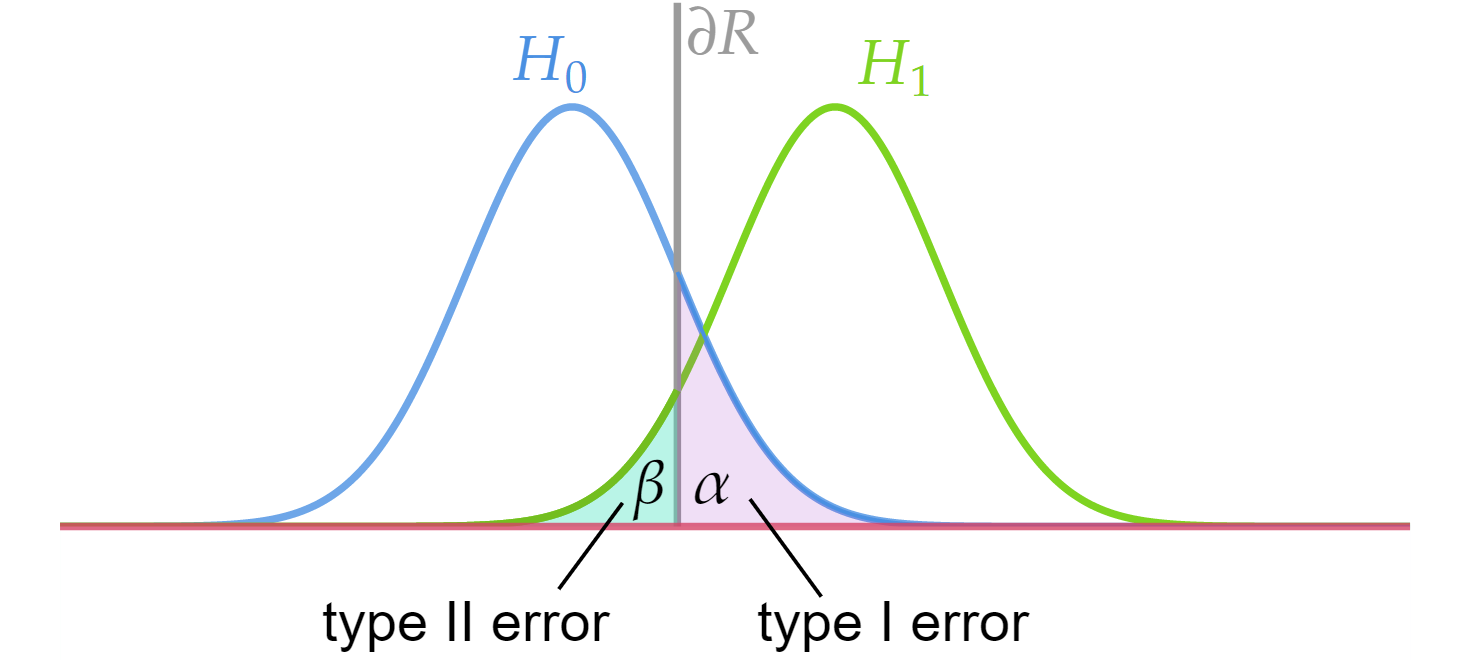
\includegraphics[width=0.55\linewidth]{sections/images/2022-09-05-16-16-51.png}
        \caption{Illustration of type I\&II error}
        \label{}
    \end{figure}
    

        
\begin{point}
        \textbf{Neyman-Pearson Principle}\index{Neyman-Pearson Principle}: First control $\alpha\leq\alpha_0$, then take $\min \beta$.
\end{point}


        How to determine $\alpha_0$? Depend on specific problem.\footnote{In most cases, take $\alpha_0=0.05$.}

        \item $p$-value: probability to get larger bias than observed $\vec{x}_0$ \uline{under $H_0$.}
        
        e.g. For reject region $R=\{\vec{X}|T(\vec{X})\geq C\},$ $p$-value:
        \begin{equation}
            p_{H_0}(\vec{x})=\mathbb{P}[T(\vec{X})\geq t(\vec{x}_0)|H_0]
        \end{equation}


        Remark: We believe that sample should reflect the property of model parameter, and $ p $-value is that under $H_0$, the probability to get a \textbf{worse} result than $\vec{x}$.
        
        Rule: Reject $H_0$ if $p(\vec{x}_0)\leq\alpha_0$.

        Note: $ p $-value is \textbf{different from} $ \alpha $ or type I error. $ p $-value is generated before we make decision while $ \alpha  $ arises after we decide how to make decisions. (But they do target the same result.)

        \item Power Function\index{Power Function}: (when $H_0$ is given), probability to reject $H_0$ by sampling.
        \begin{equation}
            \pi(\theta)=\begin{cases}
                \mathbb{P}(\text{type I error}),& \theta\in\Theta_0\\
                1-\mathbb{P}(\text{type II error}),& \theta\in\Theta_1
            \end{cases}
            =
            \begin{cases}
                \alpha(\theta),&\theta\in\Theta_0\\
                1-\beta(\theta),&\theta\in\Theta_1
            \end{cases}
        \end{equation}

        Express as test function:
        \begin{equation}
            \pi(\theta)=\mathbb{E}[\varphi(\vec{X})|\theta]
        \end{equation}

        A nice test: $\pi(\theta)$ small under $H_0$, large under $H_1$ (and grows very fast at the boundary of $ H_0 $ and $ H_1 $).
        \end{itemize}

        \begin{point}
            \textbf{General Steps of Hypothesis Testing:}
        \end{point}
        
        

        \begin{enumerate}[topsep=0pt]
            \item Propose $H_0\,\&\, H_1$.
            \item Determine $R$ (usually in the form of a statistic, e.g. $R=\{\vec{X}:T(\vec{X})\geq c\}$).
            \item Select a proper $\alpha$ (to determine $c$).
            \item Sampling, get sample (as well as $t(\vec{x})$), then 
            \begin{itemize}[topsep=-1pt,itemsep=-2pt]
                \item compare with $R$ and determine whether to reject/accept $H_0$, or
                \item calculate $ p $-value and determine whether to reject/accept$ H_0 $
            \end{itemize}
            
                
            

        \end{enumerate}

% \subsubsection{Hypotheses Testing for Common Distributions}
%     \begin{itemize}
%         \item Single normal distribution: $\vec{X}=(X_1,X_2,\ldots,X_n)$ i.i.d. from $N(\mu,\sigma^2)$
        
%         Testing $\mu$:


%     \end{itemize}

\subsubsection{Hypothesis Testing of Common Distributions}\label{SubSectionHypothesisTestingOfCommonDistributions}
    For some common distribution populations, determine rejection region $R$ under certain $H_0$ with confidence coefficient $\alpha$.

    Definition of necessary statistics see section {\autoref{SubSectionConfidenceIntervalForDistributions}}.

    \begin{enumerate}
        \item Single normal population:\index{t-test@$ t $-test}

        \begin{table}[H]
            \centering
            \renewcommand\arraystretch{1.2}
            \begin{tabularx}{\linewidth}{|c|c|c|Y|c|}
                \hline
                Condition&$H_0$&$H_1$&Testing Statistic $T$&Rejection Region $R$\\
                \hline
                \multirow{3}{*}{$\sigma^2$ known, test $\mu$}&$\mu=\mu_0$&$\mu\neq\mu_0$&\multirow{3}{*}{$T=\dfrac{\sqrt{n}(\bar{X}-\mu_0)}{\sigma}\sim N(0,1)$}&$|T|>N_\frac{\alpha}{2}$\\
                &$\mu\leq\mu_0$&$\mu>\mu_0$&&$T>N_\alpha$\\
                &$\mu\geq\mu_0$&$\mu<\mu_0$&&$T<-N_\alpha$\\
                \hline
                \multirow{3}{*}{$\sigma^2$ unknown, test $\mu$}&$\mu=\mu_0$&$\mu\neq\mu_0$&\multirow{3}{*}{$T=\dfrac{\sqrt{n}(\bar{X}-\mu_0)}{S}\sim t_{n-1}$}&$|T|>t_{n-1,\frac{\alpha}{2}}$\\
                &$\mu\leq\mu_0$&$\mu>\mu_0$&&$T>t_{n-1,\alpha}$\\
                &$\mu\geq\mu_0$&$\mu<\mu_0$&&$T<-t_{n-1,\alpha}$\\
                \hline
                \multirow{3}{*}{$\mu$ known, test $\sigma^2$}&$\sigma^2=\sigma_0^2$&$\sigma^2\neq\sigma_0^2$&\multirow{3}{*}{$T=\dfrac{nS_\mu^2}{\sigma_0^2}\sim \chi_n^2$}&$T<\chi^2_{n,1-\frac{\alpha}{2}}\cup T>\chi^2_{n,\frac{\alpha}{2}}$\\
                &$\sigma^2\leq\sigma_0^2$&$\sigma^2>\sigma_0^2$&&$T>\chi^2_{n,\alpha}$\\
                &$\sigma^2\geq\sigma_0^2$&$\sigma^2<\sigma_0^2$&&$T<\chi^2_{n,1-\alpha}$\\
                \hline
                \multirow{3}{*}{$\mu$ unknown, test $\sigma^2$}&$\sigma^2=\sigma_0^2$&$\sigma^2\neq\sigma_0^2$&\multirow{3}{*}{$T=\dfrac{(n-1)S^2}{\sigma_0^2}\sim \chi_{n-1}^2$}&$T<\chi^2_{n-1,1-\frac{\alpha}{2}}\cup T>\chi^2_{n-1,\frac{\alpha}{2}}$\\
                &$\sigma^2\leq\sigma_0^2$&$\sigma^2>\sigma_0^2$&&$T>\chi^2_{n-1,\alpha}$\\
                &$\sigma^2\geq\sigma_0^2$&$\sigma^2<\sigma_0^2$&&$T<\chi^2_{n-1,1-\alpha}$\\
                \hline
            \end{tabularx}
        \end{table}


    \item Double normal population:
    
    \begin{table}[htbp]
        \centering
        \renewcommand\arraystretch{1.2}
        \begin{tabularx}{\linewidth}{|c|c|c|Y|c|}
            \hline
            Condition&$H_0$&$H_1$&Testing Statistic $T$&Rejection Region $R$\\
            \hline
            \multirow{3}{*}{\makecell{$\sigma_1^2,\sigma_2^2$ known,\\test $\mu_1-\mu_2$}}&$\mu_1-\mu_2=\mu_0$&$\mu_1-\mu_2\neq\mu_0$&\multirow{3}{*}{$T=\dfrac{\bar{X}-\bar{Y}-\mu_0}{\sqrt{\dfrac{\sigma_1^2}{m}+\dfrac{\sigma_2^2}{n}}}\sim N(0,1)$}&$|T|>N_\frac{\alpha}{2}$\\
                &$\mu_1-\mu_2\leq\mu_0$&$\mu_1-\mu_2>\mu_0$&&$T>N_\alpha$\\
                &$\mu_1-\mu_2\geq\mu_0$&$\mu_1-\mu_2<\mu_0$&&$T<-N_\alpha$\\
                \hline
                \multirow{3}{*}{\makecell{$\sigma_1^2,\sigma_2^2$ unknown,\\test $\mu_1-\mu_2$}}&$\mu_1-\mu_2=\mu_0$&$\mu_1-\mu_2\neq\mu_0$&\multirow{3}{*}{\makecell{$T=\dfrac{\bar{X}-\bar{Y}-\mu_0}{S_\omega}\sqrt{\dfrac{mn}{m+n}}$\\$\sim t_{m+n-2}$}}&$|T|>t_{m+n-2,\frac{\alpha}{2}}$\\
                &$\mu_1-\mu_2\leq\mu_0$&$\mu_1-\mu_2>\mu_0$&&$T>t_{m+n-2,\alpha}$\\
                &$\mu_1-\mu_2\geq\mu_0$&$\mu_1-\mu_2<\mu_0$&&$T<-t_{m+n-2,\alpha}$\\
                \hline
                \multirow{3}{*}{\makecell{$\mu_1,\mu_2$ known,\\test $\dfrac{\sigma^2_1}{\sigma_2^2}$}}&$\sigma_1^2=\sigma_2^2$&$\sigma_1^2\neq\sigma_2^2$&\multirow{3}{*}{$T=\dfrac{S_{\mu_2}^2}{S_{\mu_1}^2}\sim F_{n,m}$}&\makecell{$T<F_{n,m,1-\frac{\alpha}{2}}$\\$\cup \,T>F_{n,m,\frac{\alpha}{2}}$}\\
                &$\sigma_1^2\geq\sigma_2^2$&$\sigma_1^2<\sigma_2^2$&&$T>F_{n,m,\alpha}$\\
                &$\sigma_1^2\leq\sigma_2^2$&$\sigma_1^2>\sigma_2^2$&&$T<F_{n,m,1-\alpha}$\\
                \hline
                \multirow{3}{*}{\makecell{$\mu_1,\mu_2$ unknown,\\test $\dfrac{\sigma^2_1}{\sigma_2^2}$}}&$\sigma_1^2=\sigma_2^2$&$\sigma_1^2\neq\sigma_2^2$&\multirow{3}{*}{$T=\dfrac{S_{2}^2}{S_{2}^2}\sim F_{n-1,m-1}$}&\makecell{$T<F_{n-1,m-1,1-\frac{\alpha}{2}}$\\$\cup\, T>F_{n-1,m-1,\frac{\alpha}{2}}$}\\
                &$\sigma_1^2\geq\sigma_2^2$&$\sigma_1^2<\sigma_2^2$&&$T>F_{n-1,m-1,\alpha}$\\
                &$\sigma_1^2\leq\sigma_2^2$&$\sigma_1^2>\sigma_2^2$&&$T<F_{n-1,m-1,1-\alpha}$\\
                \hline
        \end{tabularx}
    \end{table}

    \item None normal population:
    
    \begin{table}[htbp]
        \centering
        \renewcommand\arraystretch{1.7}
        \begin{tabularx}{\linewidth}{|c|c|c|Y|c|}
            \hline
            Condition&$H_0$&$H_1$&Testing Statistic $T$&Rejection Region $R$\\
            \hline
            \makecell{$\vec{X}$ from $B(1,p)$, test $p$}&$p=p_0$&$p\neq p_0$&$T=\dfrac{\sqrt{n}(\bar{X}-p_0)}{\sqrt{p_0(1-p_0)}}\xrightarrow[]{\mathscr{L}}N(0,1)$&$|T|>N_\frac{\alpha}{2}$\\
            \hline
            \makecell{$\vec{X}$ from $P(\lambda)$, test $\lambda$}&$\lambda=\lambda_0$&$\lambda\neq \lambda_0$&$T=\dfrac{\sqrt{n}(\bar{X}-\lambda_0)}{\sqrt{\lambda_0}}\xrightarrow[]{\mathscr{L}}N(0,1)$&$|T|>N_\frac{\alpha}{2}$\\
            \hline
        \end{tabularx}
    \end{table}
    \item More than two normal population: Analysis of Variance.
\end{enumerate}

\subsubsection{Likelihood Ratio Test}\label{SubSectionLRT}
    \index{LRT (Likelihood Ratio Test)}
    Idea: To test $H_0:\theta\in\Theta_0\longleftrightarrow H_1:\theta\in\Theta_1$ known $\vec{x}$, examine the likelihood function $L(\theta;\vec{x})$ and \textbf{compare} $L_{\theta\in\Theta_0}$ and $L_{\theta\in\Theta}$ to see the likelihood that $H_0$ is true.

    Def. \textbf{Likelihood Ratio} (LR):
    \begin{equation}
    \Lambda (\vec{x})=\dfrac{{\displaystyle\sup_{\theta\in\Theta_0}L(\theta;\vec{x})}}{{\displaystyle\sup_{\theta\in\Theta}L(\theta;\vec{x})}}
    \end{equation}

    Reject $H_0$ if $\Lambda(\vec{x})<\Lambda_0$. Or equivalently: Reject $H_0$ if $-2\ln\Lambda(\vec{x})>C(=-2\ln\Lambda_0)$.

    where $\Lambda_0$ (or equivalently $C=-2\ln\Lambda_0$) satisfies:
    \begin{equation}\mathbb{E}_{\Theta_0}[\varphi(\vec{X})]\leq\alpha,\quad\forall\theta\in\Theta_0\end{equation}

    LR and sufficient statistic: $\Lambda(\vec{x})$ can be expressed as $\Lambda(\vec{x})=\Lambda^*(T(\vec{x}))$, where $T(\vec{X})$ is sufficient statistic. We usually denote $ \lambda =\log \Lambda  $


\begin{point}
    LRT for one-sample $ t $-test: For $ X_1,X_2,\ldots,X_n $ i.i.d. $ \sim N(\mu,\sigma ^2) $, test

\[
    H_0: \mu=\mu_0\longleftrightarrow H_1:\mu\neq\mu_0\quad\text{when }\sigma ^2\text{ unknown}
\]

    Can prove:
    \[
        \lambda ^{2/n}=\dfrac{\sum\limits_{i=1}^n(x_i-\bar{x})^2}{\sum\limits_{i=1}^n(x_i-\mu_0)^2} 
    \]
    
    Denote $ T=\dfrac{\sqrt{n}(\bar{x}-\mu_0)}{S}$, then LRT could be expressed in equivalent form 
    \[
        \lambda  = \left( 1+\dfrac{T^2}{n-1} \right)^{-n/2}
    \]
    
    The Multivariate case see {\autoref{SubSectionMultivariateHypothesisTesting}}, where $ T^2 $ itself is the Hotelling's $ T^2 $ statistic.
    
    

\end{point}



\begin{point}
    Limiting Distribution of LRT: Wilks' Thm.\index{Wilk's Thm.}
\end{point}

    

    
    If $\dim\Theta=k>\dim\mathrm{span}\{\Theta_0\}=s$\footnote{Here 'dimension' refers to 'degree of freedom'.}, then under $H_0:\theta\in\Theta_0$:
    \begin{equation}
        -2\lambda =-2\ln \Lambda (\vec{x})\xrightarrow[]{\mathscr{L}}\chi_{k-s}^2
    \end{equation}

\subsubsection{Uniformly Most Powerful Test}\label{SUbSectionUMP}
    \index{UMPT (Uniformly Most Powerful Test)}Idea: Neyman-Pearson Principle: control $\alpha$, find $\min\beta$. i.e. control $\alpha$, find $\max\pi(\theta)$

    Def. \textbf{Uniformly Most Powerful Test} (UMP) $\varphi_{\mathrm{UMP}}$ with level of significance $\alpha$ satisfies
    \begin{equation}
        \pi_{\mathrm{UMP}}(\theta)\geq\pi(\theta),\,\forall\theta\in\Theta_1
    \end{equation}

    \textbf{Neyman-Pearson Lemma}\index{NP-Lemma (Neyman-Pearson Lemma)}: For $\vec{X}=(X_1,X_2,\ldots,X_n)$ i.i.d. from $f(\vec{x};\theta)$. 
    
    Test hypothesis $H_0:\theta=\theta_0\longleftrightarrow H_1:\theta=\theta_1$. Def. test function $\varphi$ as:
    \begin{equation}\label{UMPtestfunction}
        \varphi(\vec{x})=\begin{cases}
            1,&\dfrac{f(\vec{x};\theta_1)}{f(\vec{x};\theta_0)}>C\\
            r,&\dfrac{f(\vec{x};\theta_1)}{f(\vec{x};\theta_0)}=C\\
            0,&\dfrac{f(\vec{x};\theta_1)}{f(\vec{x};\theta_0)}<C
        \end{cases}
    \end{equation}

    Then there exists $C$ and $r$ such that
    \begin{itemize}
        \item $\mathbb{E}[\varphi(\vec{x})|\theta_0]=\mathbb{P}(\dfrac{f(\vec{x};\theta_1)}{f(\vec{x};\theta_0)}>C)+r\mathbb{P}(\dfrac{f(\vec{x};\theta_1)}{f(\vec{x};\theta_0)}=C)=\alpha$
        \item This $\varphi$ is UMP of level of significance $\alpha$
    \end{itemize}

    Actually kind of $1$-dimensional case of LRT.

    Note: UMT exist for\textbf{ simple }$H_0,H_1$, otherwise may not exist.

    UMP and sufficient statistics: Test function $\varphi(\vec{X})$ given by \autoref{UMPtestfunction} is function of sufficient statistics $T(\vec{X})$, i.e. $\varphi(\vec{X})=\varphi^*(T(\vec{X}))$.

    UMP and Exponential Family: For sample $\vec{X}=(X_1,X_2,\dots,X_n)$ from exponential family:
    \begin{equation}
    f(\vec{x};\theta)=C(\theta)h(\vec{x})\exp\{Q(\theta)T(\vec{x})\}    
    \end{equation}

    Test single hypothesis $H_0:\theta=\theta_0\longleftrightarrow H_1:\theta=\theta_1$, (where $ \theta_0<\theta_1 $ ).
    If 
    \begin{itemize}[topsep=0.5pt,itemsep=0pt]
        \item $\theta_0$ is inner point of $\Theta$
        \item $Q(\theta)$  monotone increase with $\theta$
    \end{itemize}

    Then UMP exists, in the form of:
    \begin{equation}\label{UMPtestfunctioninExponentialFamily}
            \varphi(\vec{x})=\begin{cases}
        1,&T(\vec{x})>C\\
        r,&T(\vec{x})=C\\
        0,&T(\vec{x})<C
    \end{cases} 
    \end{equation}
   
    

    where $C$ and $r$ satisfies $\mathbb{E}[\varphi(\vec{x})|\theta_0]=\alpha$.

    Note: or take $Q(\theta)$ mono decreased, then in \autoref{UMPtestfunctioninExponentialFamily}, take opposite inequality operators.
    
\begin{point}
    \textbf{General Steps of UMP}:
\end{point}

    
    \begin{enumerate}
        \item Find a point $\theta_0\in\Theta_0$ and a point $\theta_1\in\Theta_1$. (Note: \textbf{one} point)
        \item Construct test function in the form of {\autoref{UMPtestfunction}}, use $\mathbb{E}[\varphi(\vec{x})|\theta_0]=\alpha$ to determine $C$ and $r$.
        \item Get $R$ and $\varphi(\vec{x})$.
        \item If $\varphi$ does \textbf{not} depend on $\theta_1$, then $H_1$ can be generalized to $H_1:\theta\in\Theta_1$.
        \item If $\varphi$ satisfies $\mathbb{E}_{\theta\in\Theta_0}(\varphi)\leq\alpha$, then $H_0$ an be generalized to $H_0:\theta\in\Theta_0$.
    \end{enumerate}

\subsubsection{Duality of Hypothesis Testing and Interval Estimation}

\begin{itemize}
    \item Thm.: $\forall\theta_0\in\Theta$ there exists hypothesis testing $H_0:\theta=\theta_0\longleftrightarrow H_1:\theta\neq\theta_0$ of level $\alpha$ with rejection region $R_{\theta_0}$. Then
    \begin{equation}
        C(\vec{X})=\{\theta:\vec{X}\in R^C_{\theta}\}
    \end{equation}

    is a $1-\alpha$ confidence region for $\theta$

    \item Thm.: $C(\vec{X})$ is a $1-\alpha$ confidence region for $\theta$. Then $\forall\theta_0\in C(\vec{X})$, the rejection region of hypothesis testing $H_0:\theta=\theta_0\longleftrightarrow H_1:\theta\neq\theta_0$ of level $\alpha$ satisfies
    \begin{equation}
    R^\complement_{\theta_0}=\{\vec{X}:\theta_0\in C(\vec{X})\}
    \end{equation}
\end{itemize}
    
    \begin{point}
        Idea:
    \end{point}
    
        
\begin{itemize}[itemsep=-3pt]
    \item[] \centering $H_0:\theta=\theta_0\longleftrightarrow H_1:\theta\neq\theta_0$
    \begin{equation}\updownarrow\end{equation}
    \item[] \centering $\mathbb{P}(R^\complement(\vec{X})|H_0)=\mathbb{P}(R^\complement(\vec{X})|\theta_0)=1-\alpha$
    \begin{equation}\updownarrow\end{equation}
    \item[] Confidence Interval: $\theta_0\in R^\complement(\vec{X})$
\end{itemize}

    Similar for Confidence Limit and One-Sided Testing.

\subsubsection{Introduction to Non-Parametric Hypothesis Testing}\label{SubSectionIntroToNonParametricHypothesisTesting}

    Motivation: Usually distribution form unknown, cannot use parametric hypothesis testing.

    Useful Method:
    \begin{itemize}
        \item Sign Test: Used for paired comparison $\vec{X}=(X_1,X_2,\ldots,X_n)$, $\vec{Y}=(Y_1,Y_2,\ldots,Y_n)$.
        
        Take $Z_i=Y_i-X_i$ i.i.d., denote $E(Z)=\mu$. Test $H_0:\mu=0\longleftrightarrow H_1:\mu\neq 0$.

        Denote $n_+=\#(\text{positive } Z_i)$ and $n_-=\#(\text{negative }Z_i)$, $n_0=n_++n_-$. Then $n_+\sim B(n_0,\theta)$, test $H_0:\theta=\dfrac{1}{2}\longleftrightarrow H_1:\theta\neq\dfrac{1}{2}$
        
        Then use Binomial Testing or large sample CLT Normal Testing.

        Remark:
        \begin{itemize}
            \item Also can test $H_0:\theta\leq\dfrac{1}{2}\longleftrightarrow H_1:\theta>\dfrac{1}{2}$
            \item Drawback: ignores magnitudes.
        \end{itemize}
        
        \item \index{WSRT (Wilcoxon Signed Rank Sum Test)}Wilcoxon Signed Rank Sum Test: Improvement of Sign Test. Base on order statistics.
        
        Order Statistics of $Z_i$: $Z_{(1)}<Z_{(2)}<\ldots<Z_{(n)}$, where each $Z_{(j)}$ corresponds to some $Z_i$, denote as $Z_i=Z_{(R_i)}$, then $R_i$ is the rank of $Z_i$.\footnote{If some $X_i,X_j,\ldots$ equal, then take same rank $R=\mathrm{mean}\{R_i,R_j,\ldots\}$.}
        
        Def. $\vec{R}=(R_1,R_2,\ldots,R_n)$ is \textbf{Rank Statistics} of $(Z_1,Z_2,\ldots,Z_n)$

        Def. \textbf{Sum of Wilcoxon Signed Rank}: 
        \begin{equation}
        W^+=\sum_{i=1}^{n_0}R_i\mathbb{I}_{Z_i>0} 
        \end{equation}

        Distribution of $W^+$ is complex. $E$ and $var$ of $W^+$ under $H_0$:
        \begin{equation}
            \mathbb{E}(W^+)=\frac{n_0(n_0+1)}{4}\qquad var(W^+)=\frac{n_0(n_0+1)(2n_0+1)}{24}    
        \end{equation}

        Usually consider large sample CLT, construct normal approximation:
        \begin{equation}
            T=\frac{W^+-\mathbb{E}(W^+)}{\sqrt{var(W^+)}}\xrightarrow[]{\mathscr{L}}N(0,1)
        \end{equation}

        Rejection Region: $R=\{|T|>N_\frac{\alpha}{2}\}$

        \item Wilcoxon Two-Sample Rank Sum Test: Used for two independent sample comparison.\index{Wilcoxon Two-Sample Rank Sum Test}
        
        Assume $\vec{X}=(X_1,\ldots,X_m)$ i.i.d. $\sim f(x)$; $\vec{Y}=(Y_1,\ldots,Y_n)$ i.i.d. $\sim f(x-\theta)$, test $H_0:\theta=0\longleftrightarrow H_1:\theta\neq 0$.

        Rank $X_i$ and $Y_i$ as:
        \begin{equation}
            Z_1\leq Z_2\leq\ldots\leq Z_{m+n}
        \end{equation}

        in which denote rank of $Y_i$ as $R_i$, and def. \textbf{Wilcoxon two-sample rank sum}:
        \begin{equation}W=\sum_{i=1}^n R_i\end{equation}

        $\mathbb{E}$ and $var$ of $W$ under $H_0$:
\begin{equation}\mathbb{E}(W)=\frac{n(m+n+1)}{2}\qquad var(W)=\frac{mn(n+m+1)}{12}\end{equation}

        Use large sample approximation, construct CLT:
        \begin{equation}
            T=\frac{W-\mathbb{E}(W)}{\sqrt{var(W)}}\xrightarrow[]{\mathscr{L}}N(0,1)
        \end{equation}







        \item Goodness-of-Fit Test: For $\vec{X}=(X_1,X_2,\ldots,X_n)$ i.i.d. from some certain population $X$. Test $H_0:X\sim F(x)$.\index{Goodness-of-Fit Test}
        
        where $F$ is theoretical distribution, can be either parametric or non-parametric.

        Idea: Define some \textit{quantity} $D=D(X_1,\ldots,X_n;F)$ to measure the difference between $F$ and sample. And def. \textit{Goodness-of-fit} when observed value of $D$ (say $d_0$) is given:
        \begin{equation}p(d_0)=\mathbb{P}(D\geq d_0|H_0)\end{equation}

        \textbf{Goodness-of-Fit Test}: Reject $H_0$ if $p(d_0)<\alpha$.


            Pearson $\chi^2$ Test: Usually used for discrete case. 
            
            Test $H_0:\mathbb{P}(X_i=a_i)=p_i,\, i=1,2,\ldots,r$. Denote $\#(X_j=a_i)=\nu_i$, take $D$ as:
            \begin{equation}\label{Pearson_chi_test_differenceKn}
                K_n=K_n(X_1,\ldots,X_n;F)=\sum_{i=1}^r\frac{(\nu_i-np_i)^2}{np_i}
            \end{equation}

            Pearson Thm.: For $K_n$ defined as \autoref{Pearson_chi_test_differenceKn}, then under $H_0$:
            \begin{equation}
                K_n\xrightarrow[]{\mathscr{L}}\chi^2_{r-1-s}
            \end{equation} 

            Here $s$ is number of unknown parameter, $r-1-s$ is the degree of freedom.

            Note:
            \begin{itemize}
                \item $a_i$ must \textbf{not} depend on sample.
                \item For continuous case, construct division:
                \begin{equation}\mathbb{R}\rightarrow(-\infty,a_1,a_2,\ldots,a_{r-1},\infty=a_r) \end{equation}

                and test $H_0:\mathbb{P}(X\in I_j)=p_j$

                Criterion: Pick proper interval so that $np_i$ and $\nu_i$ both $\geq 5$.
            \end{itemize}
 


        \item Contingency Table Independence \& Homogeneity Test
        \index{Contingency Table}
 
\begin{itemize}
    \item Independence Test:\index{Pearson's $ \chi^2 $ Test}
    
    Test a two-parameter sample and to see whether these two parameters(features) are independent. Denote $Z=(X,Y)$ are some 'level' of sample, $n_{ij}$ is number of sample with level $(i,j)$

    Contingency Table:
    \begin{table}[H]
        \centering
        \begin{tabular}{|c|ccccc|c|}
            \hline
            \diagbox{X}{Y}&1&$\ldots$&$j$&$\ldots$&$s$&$\sum$\\
            \hline
            1&$n_{11}$&$\ldots$&$n_{1j}$&$\ldots$&$n_{1s}$&$n_{1\cdot}$\\
            $\vdots$&$\vdots$&$\ddots$&$\vdots$&$\ddots$&$\vdots$&$\vdots$\\
            $i$&$n_{i1}$&$\ldots$&$n_{ij}$&$\ldots$&$n_{is}$&$n_{i\cdot}$\\
            $\vdots$&$\vdots$&$\ddots$&$\vdots$&$\ddots$&$\vdots$&$\vdots$\\
            $r$&$n_{r1}$&$\ldots$&$n_{rj}$&$\ldots$&$n_{rs}$&$n_{r\cdot}$\\
            \hline
            $\sum$&$n_{\cdot 1}$&$\ldots$&$n_{\cdot j}$&$\ldots$&$n_{\cdot s}$&$n$\\
            \hline
        \end{tabular}
    \end{table}

        Test $H_0:X\,\&\, Y$ are independent. i.e. $H_0:P(X=i,Y=j)=P(X=i)P(Y=j)=p_{i\cdot}p_{\cdot j}$.

        Construct $\chi^2$ test statistic:
        \begin{equation}
            K_n=\sum_{i=1}^r\sum_{j=1}^s\frac{[n_{ij}-n(\frac{n_{i\cdot}}{n})(\frac{n_{\cdot j}}{n})]^2}{n(\frac{n_{i\cdot}}{n})(\frac{n_{\cdot j}}{n})}=n\left(\sum_{i=1}^r\sum_{j=1}^s\frac{n_{ij}^2}{n_{i\cdot}n_{\cdot j}}-1\right)
        \end{equation}

        Then under $H_0$, $K_n\xrightarrow[]{\mathscr{L}}\chi^2_{rs-1-(r+s-2)}=\chi^2_{(r-1)(s-1)}$

        Reject $H_0$ if $p(k_0)=P(K_n\geq k_0)<\alpha$


        \item Homogeneity Test:
        
        Test $R$ groups of sample with category rank, to see whether these groups has similar rank distribution.

        \begin{table}[H]
            \centering
            \begin{tabular}{|c|ccccc|c|}
                \hline
                \diagbox{Group}{Category}&Category 1&$\ldots$&Category $j$&$\ldots$&Category $C$&$\sum$\\
                \hline
                Group 1&$n_{11}$&$\ldots$&$n_{1j}$&$\ldots$&$n_{1C}$&$n_{1\cdot}$\\
                $\vdots$&$\vdots$&$\ddots$&$\vdots$&$\ddots$&$\vdots$&$\vdots$\\
                Group $i$&$n_{i1}$&$\ldots$&$n_{ij}$&$\ldots$&$n_{iC}$&$n_{i\cdot}$\\
                $\vdots$&$\vdots$&$\ddots$&$\vdots$&$\ddots$&$\vdots$&$\vdots$\\
                Group $R$&$n_{R1}$&$\ldots$&$n_{Rj}$&$\ldots$&$n_{RC}$&$n_{R\cdot}$\\
                \hline
                $\sum$&$n_{\cdot 1}$&$\ldots$&$n_{\cdot j}$&$\ldots$&$n_{\cdot C}$&$n$\\
                \hline
            \end{tabular}
        \end{table}


    Denote $P(\text{Category }j|\text{Group }i)=p_{ij}$. Test $H_0:p_{ij}=p_j,\,\forall 1\leq i\leq R$.

    Construct $\chi^2$ test statistic:
    \begin{equation}
        D=\sum_{i=1}^R\sum_{j=1}^C\frac{[n_{ij}-n(\frac{n_{i\cdot}}{n})(\frac{n_{\cdot j}}{n})]^2}{n(\frac{n_{i\cdot}}{n})(\frac{n_{\cdot j}}{n})}=n\left(\sum_{i=1}^R\sum_{j=1}^C\frac{n_{ij}^2}{n_{i\cdot}n_{\cdot j}}-1\right)
    \end{equation}

    Then under $H_0$, $D\xrightarrow[]{\mathscr{L}}\chi^2_{R(C-1)-(C-1)}=\chi^2_{(R-1)(C-1)}$
    \end{itemize}

    \item \hypertarget{testofnormality}{Test of Normality}: normality is a good \& useful assumption.
    
    For $\vec{Y}=(Y_1,Y_2,\ldots,Y_n)$,

    Test $H_0:\text{exists }\mu\,\&\, \sigma^2$ such that $Y_i$ i.i.d. $\sim N(\mu,\sigma^2)$.

    \begin{itemize}
        \item Kolmogorov-Smirnov Test\index{K-S Test (Kolmogorov-Smirnov Test)}: Assume $\vec{X}$ form population CDF $F(x)$, test $H_0:F(x)=F_0(x)$(where can take $F_0=\Phi$ or some other known CDF).
        
        use $F_n(x)$ (as defined in \autoref{empiricaldisreibutionfunction}) as approx. to $F(x)$, test
        \begin{equation}
            D_n=\sum_{-\infty< x<+\infty}|F_n(x)-F_0(x)|
        \end{equation}

        Reject $H_0$ if $D_n>c$

        or use goodness-of-fit: denote observed value of $D_n$ as $d_n$. Reject $H_0$ if
        \begin{equation}
            p(d_n)=\mathbb{P}(D_n>d_n|H_0)<\alpha
        \end{equation}

        \item Shapiro-Wilk Test:\index{S-W Test (Shapiro-Wilk Test)}
        
        Test $H_0:\text{exists }\mu\,\&\, \sigma^2$ such that $X_i$ i.i.d. $\sim N(\mu,\sigma^2)$.

        Denote $Y_{(i)}=\dfrac{X_{(i)}-\mu}{\sigma}$, $m_i=\mathbb{E}(Y_{(i)})$

        Under $H_0$, $(X_{(i)},m_i)$ falls close to straight line. Test Statistic: Correlation
        \begin{equation}
            R^2=\dfrac{\left(\sum_{i=1}^n(X_{(i)}-\bar{X})(m_i-\bar{m})\right)^2}{\sum_{i=1}^n(X_{i}-\bar{X})^2\sum_{i=1}^n(m_i-\bar{m})^2}=corr(X_{(i)},m_i)
        \end{equation}

        Reject $H_0$ if $R^2<c$

        Shapiro-Wilk correction:
        \begin{equation}
            W=\dfrac{\left(\sum_{i=1}^{[n/2]}a_i(X_{(n+1-i)}-X_{(i)})\right)^2}{\sum_{i=1}^n(X_{(i)}-\bar{X})^2}
        \end{equation}
    \end{itemize}
\end{itemize}

\begin{point}
    Summary: Useful Non-Parameter Hypothesis Testing.
\end{point}
\\
\\

\begin{equation*}
    \text{\makecell{Non-Parameter\\Hypothesis Testing}}
    \smash[htbp]{
    \begin{cases}
        \text{One Population Sample}
            \smash[t]{
                \begin{cases}
                    \chi^2\text{ Test}\\
                    \text{Binomial Test}\\
                    \text{One-Sample K-S Test}\\
                    \text{Wilcoxon Sign Test}\\
                    \text{Runs Test}
                \end{cases}
            }\\
            \\
            \\
            \\
            \\
        \text{Two Population Sample}
            \smash[t]{
                \begin{cases}
                    \text{Independent Sample}
                    \smash[t]{
                        \begin{cases}
                            \text{Mann-Whitney Test}\\
                            \text{K-S Test}\\
                            \text{Wald-Wolfowitz Test}\\
                            \text{Moses Test of Extreme Reactions}
                        \end{cases}
                    }\\
                    \\
                    \text{Relative Sample}
                    \smash[b]{
                        \begin{cases}
                            \text{Sign Test}\\
                            \text{McNemar Test}\\
                            \text{Wilcoxon Rank Sum Test}\\
                            \text{Marginal Homogeneity Test}
                        \end{cases}
                    }
                \end{cases}
            }\\
            \\
            \\
            \\
        \text{Multi-Population Sample}
            \smash[b]{
                \begin{cases}
                    \text{Independent Sample}
                    \smash[t]{
                        \begin{cases}
                            \text{Median Test}\\
                            \text{K-W One-Way ANOVA Test}\\
                            \text{Jonckheere-Terpstra Test}
                        \end{cases}
                    }\\
                    \\
                    \text{Relative Sample}
                    \smash[b]{
                        \begin{cases}
                            \text{Friedman Rank Sum Test}\\
                            \text{Kendall's Coefficient of Concordance Test}\\
                            \text{Cochran Q Test}
                        \end{cases}
                    }
                \end{cases}
            }
    \end{cases}  
    }
\end{equation*}

\newpage

%  \section{R语言命令部分}
%     This part base on R x64 4.0.3 on VSCode 1.52.1

% \subsection{Basic}

\subsection{Basic Command}

\begin{table}[htbp]
    \centering
    \renewcommand\arraystretch{0.9}
    \begin{tabular}{l|l}
        \hline
        Action$\qquad\qquad\qquad\qquad\qquad\qquad\qquad$&Command$\qquad\qquad\qquad\qquad\qquad$\\
        \hline
        Get help&Hover on function name\\
        Get \textbf{example}&\lstinline|example('')|\\
        \textbf{Get} current \textbf{w}orking \textbf{d}irectory&\lstinline|getwd()|\\
        \textbf{L}i\textbf{s}t all objects&\lstinline|ls()|\\
        \textbf{R}e\textbf{m}ove objects&\lstinline|rm()|\\
        Remove all objects&\lstinline|rm(list <- ls())|\\
        Install package&\lstinline|install.packages('')|\\
        Load package&\lstinline|library('')|\\
        \hline
    \end{tabular}
\end{table}

% \subsubsection{Data Structures}
% \begin{itemize}[topsep=6pt,itemsep=4pt]
%     \item Vector: One-dimensional array
    
%     \begin{point}
%         Def. a vector
%     \end{point}
% \begin{lstlisting}[language=R]
%     myvector <- c(elements)
% \end{lstlisting}

%     Note: here \lstinline|c()| for '\textbf{c}ombine'.
    
%     \begin{point}
%         Index reference
%     \end{point}
    
% \begin{lstlisting}[language=R]
%     myvector[3]
%     myvector[c(2,4)]
%     myvector[2:4]
% \end{lstlisting}
    
%     \item Matrix: Two-dimensional array
%     \begin{point}
%         Def. a matrix
%     \end{point}
% \begin{lstlisting}[language=R]
%     mymatrix <- matrix(vector, nrow, ncol, byrow, dimname)
% \end{lstlisting}

% \begin{point}
%     Index reference
% \end{point}
% \begin{lstlisting}[language=R]
%     mymatrix[2,4]
% \end{lstlisting}


%     \item Array
%     \item \textbf{Data.Frame} 
%     \item List 
% \end{itemize}

    



% \subsection{Statistics Method}




% \subsection{Graph}



\subsection{Useful Packages}

\subsubsection{\consolas{ggplot2} package}
    \lstinline|ggplot2| for `the \textbf{G}rammar of \textbf{G}raphics \textbf{Plot}' (\textbf{2}$^\mathrm{nd}$ version). \\
    Key thought: separate statistics operation (\lstinline|stat_|) and geometric operation (\lstinline|geom_|) and other parts.

    Basic syntax structures for a \lstinline|ggplot2| figure:
\begin{lstlisting}[language=R]
ggplot(data = , aes(x = , y = , ...)) +
    geom_XXX(...) + stat_XXX(...) + ... +
    annotate(...)+ ... +
    scale_XXX(...) + coord_XXX(...) + guides(...) + theme(...)    
\end{lstlisting}


\begin{itemize}[topsep=6pt,itemsep=4pt]
    \item 
\end{itemize}

    
\begin{point}
    \lstinline|aes()| for `aesthetic': Describe how variables in the data are mapped to visual properties (aesthetics) of \lstinline|geom| layer.
\end{point}



    \lstinline|geom_| functions describes
\begin{table}[H]
    \centering
      \begin{tabular}{l|l|l}
        \hline
      Functions  & Adds  & Options \\
      \hline
      \lstinline|geom_bar()|  & Bar chart  & \lstinline|color; fill; alpha | \\
      \lstinline|geom_boxplot()|  & Box plot  & \lstinline|color; fill; alpha; notch; width | \\
      \lstinline|geom_density()|  & Density plot  & \lstinline|color; fill; alpha; linetype | \\
      \lstinline|geom_histogram()|  & Histogram  & \lstinline|color; fill; alpha; linetype; binwidth | \\
      \lstinline|geom_hline()|  & Horizontal lines  & \lstinline|color; alpha; linetype; size | \\
      \lstinline|geom_jitter()|  & Jittered points  & \lstinline|color; size; alpha; shape | \\
      \lstinline|geom_line()|  & Line graph  & \lstinline|colorvalpha; linetype; size | \\
      \lstinline|geom_point()|  & Scatterplot  & \lstinline|color; alpha; shape; size | \\
      \lstinline|geom_rug()|  & Rug plot  & \lstinline|color; side | \\
      \lstinline|geom_violin()|  & Violin plot  & \lstinline|color; fill; alpha; linetype | \\
      \lstinline|geom_vline()|  & Vertical lines  & \lstinline|color; alpha; linetype; size | \\
      \hline
      \lstinline|geom_smooth()|  & Fitted line  & \lstinline|method; formula; color; fill; linetype; size | \\
      \lstinline|geom_text()|  & Text annotations & See the help for this function \\
      \hline
      \end{tabular}
  \end{table}
  
  Some useful \lstinline|geom_| function options (More options see `R in Action P445'):
\begin{table}[H]
    \centering
    \renewcommand\arraystretch{1}
    \begin{tabular}{l|l}
        \hline
        Options&Specifies\\\hline
        \lstinline|color|&Color of points\&lines\&borders of regions.\\
        \lstinline|fill|&Color of filled areas.\\
        \lstinline|alpha|&Transparency (0-1)\\
        \lstinline|linetype|&Line pattern see table.\\%%%%
        \lstinline|size|&Size of points\&lines.\\
        \lstinline|shape|&Point shape see table.\\%%%%%
        \lstinline|width|&Width of box plots.\\
        \lstinline|position|&\lstinline|dodge|/\lstinline|stack|/\lstinline|jitter| etc. position relation.\\
        \hline
        \lstinline|method|&Smoothing function to use.\\
        \lstinline|formula|&Smoothing formula, e.g. \lstinline|y~log(x)|.\\
        \lstinline|se|&Confidence interval (\lstinline|TRUE|/\lstinline|FALSE|).\\
        \lstinline|level|&Level of confidence interval.\\
    \end{tabular}
\end{table}



\lstinline|facet_| trellis command.
\begin{table}[H]
    \centering
    \renewcommand\arraystretch{1}
    \begin{tabular}{l|l}
        \hline
        \lstinline|facet_warp(~var,ncol)|&Separate plots by column.\\
        \lstinline|facet_warp(~var,nrow)|&Sparate plots by row.\\
        \lstinline|facet_grid(rowvar~colvar)|&Separate plots into combination of \lstinline|rowvar| and \lstinline|colvar|.\\
        \lstinline|facet_grid(row|&\\

        \hline
    \end{tabular}
\end{table}





\subsubsection{\consolas{data.frame} and \consolas{dplyr} package}


%  \newpage

\section{线性回归分析部分}\label{SecLinearRegressionAnalysis}
\begin{point}
    Steps in Regression Analysis
\end{point}

\begin{enumerate}[topsep=2pt,itemsep=2pt]
    \item Exploratory Data Analysis (EDA)\index{EDA (Exploratory Data Analysis)}
    \item Statement of the problem;
    \item Selection of potentially relevant variables;
    \item Data collection;
    \item Model specification;
    \item Choice of fitting method;
    \item Model fitting;
    \item Model validation and criticism;
    \item Using the chosen model(s) for the solution of the posed problem.
\end{enumerate}

    

\subsection{Linear Regression Model}
\begin{itemize}[topsep=6pt,itemsep=4pt]
    \item Assume a Model
    \begin{enumerate}[topsep=6pt,itemsep=4pt]
        \item Parameter of the model
        \item Basic Assumptions
        \item Dsitribution of error
    \end{enumerate}
    \item Parametric Estimation
    \begin{enumerate}[topsep=6pt,itemsep=4pt]
        \item Ordinary Least Squares Estimation
        \item Maximun Likelihood Estimation
    \end{enumerate}
    \item Statistics Inference
    \begin{enumerate}[topsep=6pt,itemsep=4pt]
        \item Hypotheses Testing
        \item Interval Estimation
    \end{enumerate}

\end{itemize}


    


        
\subsubsection{Data for simple linear regression}

    We will observe pairs of variables, called 'cases'(样本点)
        
    A sample is $ (X_1,Y_1),\ldots,(X_n,Y_n) $

    Linear Model: \footnote{Here in linear regression, we consider $ X_i $ only as real number, \textbf{without} randomness. So here $ Y_i $ can be considered as an r.v. with $ X_i $ as parameter, i.e. $ Y_i|_{X_i=x_i} $}

%% 关于线性模型的X_i性质的假定
    \[
        Y_i=\beta _0+\beta _1X_i+\varepsilon _i 
    \]
    where $ \varepsilon_i  $ i.i.d.$ \sim \varepsilon  $ is a random error term, satisfies    \footnote{Note: Why we need $ \varepsilon $ as 'random error term'?
    \begin{itemize}[topsep=6pt,itemsep=4pt]
        \item It represents the intrinsic random property of the model.
        \item Based on $ \varepsilon  $, we can take r.v. into our statistic model.
    \end{itemize}
    }
    
    \[
        E(\varepsilon _i)=0\qquad var(\varepsilon _i)=\sigma ^2 
    \]
    
    

    Normal Error Assumption: Further in most cases, we consider $ \varepsilon \sim N(0,\sigma^2) $ ----because of its well-property distribution, $ \varepsilon _1,\varepsilon _2,\ldots,\varepsilon _n $ i.i.d. $ N(0,\sigma ^2) $.\footnote{i.e. $ Y_i $ are independent
    \[
        Y_i\sim N(\beta _0+\beta _1X_i,\sigma^2)\quad i=1,2,\ldots ,n 
    \]
    
    }
        
    What does Linear Regression do? Under Linear Model, try to estimate 
    \begin{itemize}[topsep=0pt,itemsep=-2pt]
        \item $ \beta _0\text{ (intercept) }$;
        \item $\beta _1\text{ (slope) }$;
        \item $\sigma ^2\text{ (variance of error)} $.
    \end{itemize}
    
    
    (Thus Linear Regression is also a Statistics Inference process: deduce properties of model from data)
        
\subsubsection{The Ordinary Least Square Estimation}
    Aim: use $ (x_i,y_i) $  to estimate $ \beta _0,\beta _1,\sigma^2 $. The idea is to define a 'loss function' to reflect the 'distance' from sample point to estimation point.

    Estimate Principle: \footnote{Detailed Definition and Derivation see sec.\ref{SubSectionMoM_MLE_LinearRegression}.}
    \begin{itemize}[topsep=2pt,itemsep=2pt]
        \item Ordinary Least Squares\index{Ordinary Least Squares}:
        \[
            (\hat{\beta  }_0,\hat{\beta _1})=\arg\min\sum_{i=1}^n (y-\beta _0-\beta _1x_i)^2
        \]
        \item MLE or MoM Estimation.
    \end{itemize}
    

    
    And get $ \hat{\beta _1},\hat{\beta _0}$ as well as $ \hat{\sigma^2} $(see eqa(\ref{EqaOLSEstimatorOfSigma}):\footnote{A memory trick: use $ \dfrac{Y}{\sqrt{s_Y}}=r_{XY}\dfrac{X}{\sqrt{s_X}} $ to get formular of $ Y\sim X $:
    \[
        \hat{\beta }_1=r_{XY}\dfrac{\sqrt{s_Y}}{\sqrt{s_X}}=\dfrac{{\displaystyle\sum (x_i-\bar{x})(y_i-\bar{y})}}{{\displaystyle\sum (x_i-\bar{x})^2}} 
    \]}

%LSE beta_0 beta_1
\begin{equation}\label{EqaOLSEstimatorOfBeta}
    \begin{aligned}
        \hat{\beta }_1=&\dfrac{\sum\limits_{i=1}^n (x_i-\bar{x})(y_i-\bar{y})}{\sum\limits_{i=1}^n (x_i-\bar{x})^2}\\
        \hat{\beta }_0=&\bar{y}-\hat{\beta _1}\bar{x}\\
        \hat{\sigma^2}=&\dfrac{1}{n-p-1}\sum_{i=1}^n(y_i-\hat{\beta }_0-\hat{\beta }_1x_i)^2
    \end{aligned}
\end{equation}


    
    Def. \index{Residual}\textbf{Residual}: distance from sample point to estimate point, to reflect how the sample points fit the model.
    \[
        e_i=y_i-\hat{y}_i=\text{observed value of }\varepsilon _i 
    \]
    
    Note: under least square estimation, we have\footnote{Intuitively, they each means '$ E(\varepsilon )=0 $' and '$ X\parallel \varepsilon  $'.}
\begin{equation}\label{Limit_to_Residual}
        \sum e_i=0\qquad \sum x_ie_i=0 
\end{equation}
    

    Then use $ e_i $ to estimate $ \sigma ^2 $ (because it is $ \varepsilon _0 $ that are i.i.d., not $ Y_i $), where $ (n-p-1) $ is Degree of Freedom (df or dof)\footnote{Generally, MLE and LSE are different.

    Comment from R.A.Fisher: $ \sum e_i^2 $ should be divided by 'number of $ e_i^2 $ that contribute to variance'. Here $ (n-p-1) $ corresponds to 'degree of freedom' $ =(n-2) $, $ p=1 $ corresponds to `one' variable (see sec.\ref{SubSectionMoM_MLE_LinearRegression}, eqa(\ref{EqaEstimatorSigmaWithDoF})), and correponds to the two equations of $ e_i $, eqa(\ref{Limit_to_Residual})}
\begin{equation}\label{EqaOLSEstimatorOfSigma}
    \begin{aligned}
        \hat{\sigma _n^2}&=\dfrac{1}{n}\sum e_i^2 \quad\text{(use MLE or MoM)}\\
        \hat{\sigma^2}&=\dfrac{1}{n-p-1}\sum e_i^2=\dfrac{1}{n-2}\sum e_i^2\quad\text{(use OLS, unbiased)}
\end{aligned}
\end{equation}

    % MSE SSE dof






    % Review: Statistical Inference
    % \begin{itemize}[topsep=6pt,itemsep=4pt]
    %     \item Basic concepts: HT CI;
    %     \item Inference about $ \beta _1$;
    %     \item Inference about $ \beta _0 $.
    % \end{itemize}

    % Note: the distribution of $ \hat{\beta }_0,\hat{\beta }_1 $ is sampling distribution(抽样分布): distribution of statistics.



    % Power function of testing
    % \begin{itemize}[topsep=6pt,itemsep=4pt]
    %     \item Definition;
    %     \item Calculation;
    %     \item Sample<->Power (Calculation of sampling).
    % \end{itemize}


\subsubsection{Statistical Inference to $ \beta _0 $,$ \beta _1 $}

\begin{point}
    Sampling Distribution of $ \hat{\beta} _1,\hat{\beta} _0  $
\end{point}

    Consider $ \hat{\beta} _1,\hat{\beta} _0 $ as statistics of sample, then we can examine the sampling distribution of $  \hat{\beta} _1,\hat{\beta} _0 $. Their randomness comes from
    \[
        Y_i=\beta_0+\beta_1X_i+\varepsilon _i 
    \]
    
    

    (The following part treats $\hat{\beta} _1,\hat{\beta} _0 $ as r.v., and note that $ X_i $ are \textbf{not }r.v.. And  for convenience and conciseness, denote $ S_{XX}={\displaystyle\sum_{i=1}^n(X_i-\bar{X})^2} $)

   
\begin{align*}
        \hat{\beta }_1&=\beta _1+\sum_{i=1}^n\dfrac{X_i-\bar{X}}{S_{XX}}\varepsilon _i\\
        \hat{\beta }_0&=\beta _0+\sum_{i=1}^n\left(\dfrac{1}{n}-\dfrac{(X_i-\bar{X})\bar{X}}{S_{XX}}\right)\varepsilon _i
\end{align*}
 
    Denote corresponding variance as $ \sigma^2_{\hat{\beta}_1} $ and $ \sigma^2_{\hat{\beta}_0} $, using eqa(\ref{EqaDistributionOfSumOfiidNormal}) to get:
    \[
        \sigma^2_{\hat{\beta}_1}= \dfrac{\sigma^2}{S_{XX}}\qquad \sigma^2_{\hat{\beta}_0}=\sigma^2(\dfrac{1}{n}+\dfrac{\bar{X}^2}{S_{XX}})
    \] 
    
     And under normal error assumption, distribution of $ \hat{\beta} _1,\hat{\beta} _0  $ are
    \begin{align*}
        \hat{\beta }_1&\sim N(\beta _1,\sigma^2_{\hat{\beta}_1}) =N(\beta_1,\dfrac{\sigma^2}{S_{XX}})\\
        \hat{\beta}_0&\sim N(\beta_0,\sigma^2_{\hat{\beta }_0}) =N(\beta_0,\sigma^2(\dfrac{1}{n}+\dfrac{\bar{X}^2}{S_{XX}}))
    \end{align*}
    
    Based on sampling distribution of $ \hat{\beta} _1,\hat{\beta} _0  $, we can conduct statistical inference, including CI and HT.\footnote{Detail see sec.\ref{SectionHypothesisTesting}, estimating/testing $ \hat{\beta} _1,\hat{\beta} _0  $ usually corresponds to 'estimate $ \mu $, with $ \sigma^2 $ unknown'.}
    
    % \begin{itemize}[topsep=2pt,itemsep=2pt]
    %     \item LSE of $ \beta _1 $ gives 
    %     \[
    %         \hat{\beta _1}=\dfrac{\sum (x_i-\bar{x})(y_i-\bar{y})}{\sum (x_i-\bar{x})^2}
    %     \]
        
    %     and satisfies $ E(\hat{\beta}_1)=\beta_1 $. Can prove that $ \hat{\beta }_1\sim N(\beta _1,\dfrac{\sigma ^2}{\sum (x_i-\bar{x})^2})=N(\beta_1,\sigma^2(\hat{\beta}_1))$
       
    % \end{itemize}
    
    Note: In linear regression model, we usually focus more on $ \beta_1 $. And note that when $ 0 $ is \textbf{not} within the fitting range,$ \beta_0 $ is not so important.\footnote{Two reason:\begin{itemize}[topsep=2pt,itemsep=2pt]
        \item The etimation error of $ Y $ from $ \hat{\beta}_1 $ increases with $ X_h-\bar{X} $;
        \item $ \beta_1==0  $ is important: decides whether linear model can be used. 
    \end{itemize}
    
        }

    Why we choose OLS to get regression coefficients?

\begin{point}
    \index{Gauss-Markov Thm.`'}Gauss–Markov Thm.: the OLS estimator has the lowest sampling variance within the class of linear unbiased estimators, i.e. OLS is the Best Linear Unbiased Estimator(BLUE).\footnote{This Thm. does \textbf{not }require normal error assumption.}
\end{point}
    



\subsubsection{Prediction to $ Y_h $}
    For a new $ X_h $ at which we wish to \textbf{predict }the corresponding $ Y_h $ (based on other known point $ (X_i,Y_i) $), denote the estimator as $ \hat{\mu}_h $:
    \[
        \hat{\mu}_h=\hat{\beta}_1X_h+\hat{\beta}_0 =\beta_1X_h+\beta _0+\sum_{i=1}^n\left( \dfrac{1}{n}+\dfrac{(X_i-\bar{X})(X_h-\bar{X})}{S_{XX}} \right)\varepsilon _i
    \]
    
    Thus we can get\footnote{So $ \sigma ^2(\hat{\mu }_h) $ increases with $ X_h-\bar{X} $. Intuitively it make sense, because $ (\bar{X},\bar{Y})$ must falls on regression line.}
    \[
        E(\hat{\mu}_h)= \beta _1X_h+\beta _0\qquad \sigma ^2_{\hat{\mu}_h}=\left( \dfrac{1}{n}+\dfrac{(X_h-\bar{X})^2}{S_{XX}} \right)\sigma^2
    \]
    
    Under Normal assumption:
    \[
        \hat{\mu}_h\sim N(\beta _1X_h+\beta _0,\left( \dfrac{1}{n}+\dfrac{(X_h-\bar{X})^2}{S_{XX}} \right)\sigma^2) 
    \]
    
    Base on distribution we can give CI and HT.

    Note: Remember that when we consider the estimator $ \hat{\mu } $, we \textbf{must } have the randomness of $ \hat{\beta }_0,\hat{\beta }_1 $ considered(if they are unknown).
    
    Prediction Error: $ Y_h $ itself is an $ Y $ of the linear model, i.e. $ Y_i=\beta_0+\beta_1X_h+\varepsilon _h $, we can consider \textbf{$ Y_h $ itself as an r.v. }v.s.\textbf{ predicted $ Y_h $ from other sample points} and define \textbf{Prediction Error}: 
    \[
        d_h=Y_h-\hat{\mu}_h 
    \]

    
    \[
        E(d_h)=0\qquad \sigma^2_{d_h}=var(Y_h-\hat{\mu }_h)=\sigma^2\left[ 1+\dfrac{1}{n}+\dfrac{(X_h-\bar{X})}{S_{XX}} \right] > \sigma ^2_{\hat{\mu}_h}
    \]
    


    \begin{point}
       Simultaneous Confidence Band(SCB)\index{SCB (Simultaneous Confidence Band)}\index{CB (Confidence Band)}
    \end{point}

    Confidence Band is \textbf{not} the CI at each point, but really a \textbf{band} for the \textbf{entire} regression line.\footnote{Why they are different? We require the confidence band have a \textbf{simultaneous} converage probability. For the same band $ (L(x),U(x)) $, $ P(\text{the whole line})< P(\text{each point})$, so Confidence Band is wider than $ \bigcup $CIs to hold the same $ 1-\alpha $.
    
    Also, we will see that for linear model, the boundary of SCB forms hyperbola, which make sense considering its asymptotic line.}
    
    
    Aim: Find lower and upper function $ L(x) $ and $ U(x) $ such that
    \[
        P[L(x)<(\beta _0+\beta _1x)<U(x),\,\forall x\in I_x]=1-\alpha  
    \]
    
    and get \textbf{Confidence Band}:
    \[
        \{(x,y)|L(x)<y<U(x)|\forall x\in I_x\} 
    \]
    
    % Note: \textbf{Cannot} use CI at each point to form Confidence Band. Band is wider. And we are actually conduce CI \textbf{simoutanesly} to all $ x $.

    Where $ (L(x),U(x)) $ can be derived as
    \[
        (L(x),U(x))=\hat{\mu}_x\pm s_{\hat{\mu}_x}W_{2,n-2,1-\alpha}
    \]

    Where $ W $ correponds to $ W $ distribution: $ W_{m,n}=\sqrt{2F_{m,n}} $
    
    
    
    Small sample case: Bonferroni correction.
    




% 
% 
% 
% 
% 
% 
% 


\subsection{Analysis of Variance}
    \index{ANOVA (Analysis of Variance)}\textbf{AN}alysis \textbf{O}f \textbf{VA}riance (ANOVA): One-sample $ t $ test$ \rightsquigarrow $ Two sample $ t $ test$ \rightsquigarrow $ ANOVA
\begin{itemize}[topsep=2pt,itemsep=2pt]
    \item Partition of Totla Sum of Squares;
    \item Partition of Degree of Freedom;
    \item MSS$ \rightsquigarrow $ F-test;
    \item ANOVA table;
    \item General linear test. --to be examined further in later sections.
    \item (Pearson) Correlation Coefficient $ \leftrightarrow \, R^2$
\end{itemize}

    SST: Total Sum of Squares\index{SST (Total Sum of Squares)}
    \[
        \mathrm{SST}=\sum_{i=1}^n(Y_i-\bar{Y})^2 
    \]
    
    Note: Here $ Y_i $ are not i.i.d. (different mean).

    Idea: take partition of SST. For instance
    \[
        Y_i-\bar{Y}=(Y_i-\hat{Y})+(\hat{Y}-\bar{Y})=e_i 
    \]
    
    Note: $ \bar{Y}=\bar{\hat{Y}} $

    then we partition SST into\footnote{\textbf{IMPORTANT: }In some books \begin{itemize}[topsep=2pt,itemsep=2pt]
        \item SSError $ \to $ SSResidual;
        \item SSRegression $ \to $ SSExplained.
    \end{itemize}

    And Cause \textbf{Confusion}! In this summary we take the former.
         }

         \begin{itemize}[topsep=2pt,itemsep=2pt]
        \item variation due to model \index{SSR (Regression Sum of Squares)}(SSRegression) (which is explained by regression line);
        \[
            \mathrm{SSR}= \sum_{i=1}^n(\hat{Y}_i-\bar{Y})^2
        \]
        
        \item variation attribtes to $ \varepsilon  $ \index{SSE (Error Sum of Squares)}(SSError).
        \[
            \mathrm{SSE}= \sum_{i=1}^n(Y_i-\hat{Y_i})
        \]
        
        
    \end{itemize}
    
    can prove
    \[
        \mathrm{SST}=\sum_{i=1}^n(Y_i-\bar{Y})^2=\sum_{i=1}^n(\hat{Y}_i-\bar{Y})^2+\sum_{i=1}^n(Y_i-\hat{Y_i})^2=\mathrm{SSR+SSE} 
    \]

    That is: we \textbf{partition} SST into two parts, so that we can examine them seperately.

    \begin{point}
        ANOVA Table\footnote{$ \mathrm{SSR}=\hat{\beta }_1^2\sum_{i=1}^n(X_i-\bar{X})^2$, so $ dof_R=1 $}
    \end{point}
    \begin{table}[H]
        \centering
        \renewcommand\arraystretch{1}
        \begin{tabular}{c|ccc}
            \hline
            Source&$ dof $&SS&MS\\
            Regression&1&$ \sum_{i=1}^n(\hat{Y}_i-\bar{Y})^2  $&SSR/$ dof_R $\\
            Error&$ n-2 $&$ \sum_{i=1}^n(Y_i-\hat{Y}_i)^2  $&SSE/$ dof_E $\\
            Total&$ n-1 $&$ \sum_{i=1}^n(Y_i-\bar{Y})^2  $&SST/$ dof_T $\\
            \hline
        \end{tabular}
    \end{table}
    
    Properties:
    
    \[
        E(\mathrm{MSE})=\sigma ^2\qquad E(\mathrm{MSR})=\sigma ^2+\beta _1^2S_{XX} 
    \]
    
\begin{point}
    Hypotheses Testing to $ H_0:\beta _1=0 $
\end{point}
\begin{itemize}[topsep=2pt,itemsep=2pt]
    \item 
    We can examine $ F=\dfrac{\mathrm{MSR}}{\mathrm{MSE}}\sim F_{dof_R,dof_E}=F_{1,n-2} $
    \item    Or: General Linear Test (GLT)\index{GLT (General Linear Test)}\begin{itemize}[topsep=2pt,itemsep=2pt]
        \item Full model: $ Y_i=\beta _0+\beta _1X_i+\varepsilon _i $.
        \item Reduced model: $ Y_i=\beta _0+\varepsilon _i $.
    \end{itemize}

    and examine
    \[
        F=\dfrac{(\mathrm{SSE_R-SSE_F})/dof_{R-F} }{\mathrm{SSE_F}/dof_F} \sim F_{dof_{R}-dof_F,dof_F}
    \]
\end{itemize}

\begin{point}
    Pearson Correlation Coefficient $ R^2 $
\end{point}

\[
    R^2=\dfrac{\mathrm{SSR}}{\mathrm{SST}} 
\]

    Note: under simple linear model, $ r^2=R^2 $, where $ r=\hat{\beta}_1\dfrac{\sigma _X}{\sigma _Y} $



\subsection{Model Assumption and Diagnostics}
    
\begin{point}
    Diagonostics to $ X $
\end{point}


    Considering the dependence of $ Y_i $ on $ X_i $, we cannot just focus on the (marginal) distribution of $ Y_i $. Thus we also need a better 'distribution' of $ X_i $
    \begin{itemize}[topsep=2pt,itemsep=2pt]
        \item 4 statistics(parameters);\footnote{See sec.\ref{SubSectionStatistics}}
        \begin{itemize}[topsep=2pt,itemsep=2pt]
            \item Mean: Location;
            \[
                \bar{X}=\dfrac{1}{n}\sum_{i=1}^nX_i 
            \]
            \item Standard Deviation: Variability;
            \[
                S^2=\dfrac{1}{n-1}\sum_{i=1}^n(X_i-\bar{X}) ^2
            \]
            
            
            \item Skewness: Lack of Symmertry;
            \[
                \hat{g}_1=\dfrac{m_{n,3}}{m_{n,2}^{3/2}}=\dfrac{\frac{1}{n}\sum\limits_{i=1}^n(X_i-\bar{X})^3}{\left( \frac{1}{n}\sum\limits_{i=1}^n(X_i-\bar{X}) \right)^{3/2}} 
            \]

            Adjusted Skewness (Least MSE):
            \[
                \dfrac{\sqrt{n(n-1)}}{n-2}\hat{g}_1 
            \]
            
            \begin{itemize}[topsep=2pt,itemsep=2pt]
                \item $ \hat{g}_1>0 $: Right skewness, longer right tail;
                \item $ \hat{g}_1<0 $: Left skewness, longer left tail.
            \end{itemize}
            
                
            Fisher-Pearson coefficient of skewness.


            \item Kurtosis: Heavy/Light Tailed.
            \[
                \hat{g}_2=\dfrac{m_{n,4}}{m_{n,2}^2}-3= \dfrac{\frac{1}{n}\sum\limits_{i=1}^n(X_i-\bar{X})^4}{\left( \frac{1}{n}\sum\limits_{i=1}^n(X_i-\bar{X}) \right)^{2}} -3
            \]

            $ \hat{g}_2=0 \Rightarrow $ similar to normal.
            \begin{itemize}[topsep=2pt,itemsep=2pt]
                \item $ \hat{g}_2>0 $: Leptokurtic, heavy tail slender;
                \item $ \hat{g}_2<0 $: Platykurtic, light tail  broad.
            \end{itemize}
            
            Note: In expression of $ \hat{g}_1 $ and $ \hat{g}_2 $, we already divide the variance. So Skewness and Kurtosis only reflect the difference from normal, but not related to variance!
                
            Best tool to determine Kurtosis: QQ-Plot.
            
        \end{itemize}
        \item Useful Plots:
        \begin{itemize}[topsep=2pt,itemsep=2pt]
            \item BoxPlot: a rough distribution.
            
            25\%-quantile$ - $ 1.5IQR$ \vdash \sqsubset  $ 25\%-quantile$ \square  $ 75\%-quantile $ \sqsupset \dashv  $ 75\%-quantile$ + $ 1.5IQR\footnote{IQR:InterQuartile Range\index{IQR (InterQuartile Range)}}

            \item Histogram Plots: Frequency distribution (can deal with many-peak)
            \item Quantile-Quantile Plots\index{QQ-Plot (Quantile-Quantile Plots)}: Examine the similarity  between distribution.
            
            For two CDF $ q=F(x) $ and $ q=G(x) $(where $ q $ for quantile), with $ x=F^{-1}(q) $, $ x=G^{-1}(q) $. And Plot $ F^{-1}(q) $-$ G^{-1}(q) $.

            Usually test normality, take $ G=\Phi  $
        \end{itemize}
        
            
        \item Normality;
        \item Bias:
        \begin{itemize}[topsep=2pt,itemsep=2pt]
            \item Selection Bias: Not completely random sampling;
            \item Information Bias: Difference between 'designed' and 'get', e.g. no response;
            \item Confounding: Exist another important variable, while the model actually focuses on a less important variable, or even reverse the causality.
        \end{itemize}
        
            
    \end{itemize}
    
\begin{point}
    Diagnostics to Residual
\end{point}

    Residual Plot: Reflect the linearity and variance assumption

    Testing of 
\begin{itemize}[topsep=2pt,itemsep=2pt]
    \item The Assumption of Equal Variances:
    \begin{itemize}[topsep=2pt,itemsep=2pt]
        \item Bartlett's test: Comes from UMPT, useful when normality assumption satisfied.
        \item Levene's test: 
        \item Brown-Forsythe test (Modified Levene's test): 
        \item Breusch-Pagan test:
    \end{itemize}


    \item The Assumption of Normality:
    \begin{itemize}[topsep=2pt,itemsep=2pt]
        \item Shapiro-Wilk Test (Most Powerful):
    \end{itemize}
    


    \item The Assumption of Independence:
        
    
        
\end{itemize}

    

    
\newpage

\section{多元统计分析部分}\label{SecMultivariateStatisticalAnalysis}
\subsection{Multivariate Data}
    In this section, we consider a \textbf{Multivariate Statistic Model}. Sample comes from $p$ dimension multivariate population $f(x_1,x_2,\ldots,x_p)$.

    \textbf{Notation }: In this section, we still denote random variable in upper case and observed value in lower case, specially express random vector in bold font. \textbf{But} in this section we usually omit the vector symbol $ \vec{\cdot} \,\,$. e.g.
    random vector with $ n $ \textbf{variable }is denoted as $\mathbf{X}=(X_{\cdot 1},X_{\cdot 2},\ldots ,X_{\cdot p})$; sample of size $ n $ from the multivariate population is a $ n\times p $ matrix $ \{x_{ij}\} $, each sample item (a row in sample matrix) is denoted as $ x_i' $ or $ x_i^T $.\footnote{Here sample item (or sample case) $x_i=[x_{i1},x_{i2},\ldots,x_{ip}]^T$ is a column vector.} 
    % In this section we use the upper case $ X_i $ means that it's a vector (not necessarily means an r.v.).
    %\footnote{In previous section, a multivariate r.v. is denoted $\vec{X}=(X_1,X_2,\ldots,X_p) $, and sample item is $ \vec{X_i}=(X_{i1},X_{i2},\ldots,X_{ip})  $}


\subsubsection{Matrix Representation}


    \begin{itemize}[topsep=0pt,itemsep=1pt]
        \item \hyperlink{RandomVariableRepresentation}{Random Variable Representation}
        \item \hyperlink{SampleRepresentation}{Sample Representation}
        \item \hyperlink{StatisticsRepresentation}{Statistics Representation}
        \item \hyperlink{SampleStatisticsProperties}{Sample Statistics Properties}
    \end{itemize}
    



\begin{point}
    \hypertarget{RandomVariableRepresentation}{Random Variable Representation}:
\end{point}
    \begin{itemize}[topsep=6pt,itemsep=4pt]
        \item Random Matrix: Definition and basic properties of r.v. see section \ref{SectionPropertiesOfRandomVariableAndVector}. Now extend the definition to matrix $ X=\{X_{ij}\} $. 
    
    \[
        X=\{X_{ij}\}=\begin{bmatrix}
        X_{11}&X_{12}&\ldots&X_{1p}\\
        X_{21}&X_{22}&\ldots&X_{2p}\\
        \vdots&\vdots&\ddots&\vdots\\
        X_{1n}&X_{n2}&\ldots&X_{np}\\
        \end{bmatrix} 
    \]

    And we can further define $ E(X)=\{E(X_{ij})\} $.
    For any const matrix $ A,B $ we have
    \[
        E(AXB)=AE(X)B 
    \]

    \item Random Vector: For a $ p\times 1 $ random vector $ \vec{X}=(X_{1},X_{2},\ldots,X_{p})^T  $, denote (Marginal) expectation and variance, and covariance, correlation coefficient between $ X_i,X_j $ as follows:
    \begin{align*}
        \mu_i&=E(X_i)\\
        \sigma _{ii}&=\sigma_i ^2=E(X_i-\mu_i)^2\\
        \sigma_{ij}&=E[(X_i-\mu_i)(X_j-\mu_j)]\\
        \rho _{ij}&=\dfrac{\sigma _{ij}}{\sqrt{\sigma _{ii}}\sqrt{\sigma _{jj}}}
    \end{align*}
    
    and we have covariance matrix (as defined in section \ref{SubSubSectionCovarianceAndCorrelation}, eqa.\ref{covariancematrix})
    \[
        \Sigma =E[(X-\mu)(X-\mu)^T] =
        \begin{bmatrix}
        \sigma _{11}&\sigma _{12}&\ldots&\sigma _{1p}\\
        \sigma _{21}&\sigma _{22}&\ldots&\sigma _{2p}\\
        \vdots&\vdots&\ddots&\vdots\\
        \sigma _{1p}&\sigma _{p2}&\ldots&\sigma _{pp}\\
        \end{bmatrix}
    \]

    and Standard Deviation Matrix
    \[
        V^{1/2}=diag\{\sqrt{\sigma _{ii}}\} 
    \]

    Based on $ \vec{X}=(X_{1},X_{2},\ldots,X_{p})  $, consider the linear combination:$ Y=c'X=c_1X_1+c_2X_2+\ldots c_pX_p $
    \begin{align*}
        E(y)=c'\mu\qquad var(Y)=c'\Sigma c
    \end{align*}

    and $ Z_i=\sum_{j=1}^p c_{ij}X_j $ (i.e. $ Z=CX $):
    \[
        \mu_Z=E(Z)= C\mu_X\qquad \Sigma _Z=C\Sigma _XC^T
    \]
    
    
    
    

    and Correlation Matrix
    \[
        \rho =\begin{bmatrix}
        \rho _{11}&\rho _{12}&\ldots&\rho _{1p}\\
        \rho _{21}&\rho _{22}&\ldots&\rho _{2p}\\
        \vdots&\vdots&\ddots&\vdots\\
        \rho _{1p}&\rho _{p2}&\ldots&\rho _{pp}\\
        \end{bmatrix} 
        =V^{-1/2}\Sigma V^{-1/2}
    \]
    
    

    
    
    
    
    
    \end{itemize}
    
        
\begin{point}
    \hypertarget{SampleRepresentation}{Sample Representation}:
\end{point}
    
    Sample of $n$ items from population characterized by $ p $ variables
    \begin{table}[H]
        \centering
        \begin{tabular}{|c|cccccc|}
            \hline
            \diagbox{Item}{Variable}&Variable 1&Variable 2&$\ldots$&Variable $j$&$\ldots$&Variable $p$\\
            \hline
            Item 1&$ x_{11} $&$ x_{12} $&$ \ldots $&$ x_{1j} $&$ \ldots $&$ x_{1p} $\\
            Item 1&$ x_{21} $&$ x_{22} $&$ \ldots $&$ x_{2j} $&$ \ldots $&$ x_{2p} $\\
            $\vdots$&$\vdots$&$\vdots$&$ \ddots $&$\vdots$&$ \ddots $&$\vdots$\\
            Item $j$&$ x_{i1} $&$ x_{i2} $&$ \ldots $&$ x_{ij} $&$ \ldots $&$ x_{ip} $\\
            $\vdots$&$\vdots$&$\vdots$&$ \ddots $&$\vdots$&$ \ddots $&$\vdots$\\            
            Item $n$&$ x_{n1} $&$ x_{n2} $&$ \ldots $&$ x_{nj} $&$ \ldots $&$ x_{np} $\\
            \hline
        \end{tabular}
    \end{table}

    Or represented in condense notation:
    \[
        X=\{x_{ij}\}=
        \begin{bmatrix}
            x_1^T\\x_2^T\\ \vdots \\ x_n^T
        \end{bmatrix}
        =
        \begin{bmatrix}
            x_{11}&x_{12}&\ldots&x_{1p}\\
            x_{21}&x_{22}&\ldots&x_{2p}\\
            \vdots&\vdots&\ddots&\vdots\\
            x_{n1}&x_{n2}&\ldots&x_{np}\\
        \end{bmatrix} 
        =
        \begin{bmatrix}
            y_1&y_2&\ldots &y_p
        \end{bmatrix}
    \]
\begin{point}
    \hypertarget{StatisticsRepresentation}{Statistics Representation}
\end{point}

    \begin{itemize}[topsep=6pt,itemsep=4pt]
        \item Unit 1 vector:
        \[
            \mathbf{1}_k=(\underbrace{1,1,\ldots,1}_{k\text{ 1 in total}})^T
        \]
        
        \item Sample mean:
        \[
            \bar{x}_i=\dfrac{x_{1i}+x_{2i}+\ldots+x_{ni}}{n}=\dfrac{y_i'\mathbf{1}_n}{n}
        \]
        
        \item Deviation of measurement of the $ i^\mathrm{th} $ variable:
        \[
            d_i=y_i-\bar{x}_i\mathbf{1}_n=\begin{bmatrix}
                x_{1i}-\bar{x}_i\\x_{2i}-\bar{x}_i\\\vdots\\x_{ni}-\bar{x}_i
            \end{bmatrix} 
        \]
        \item Covariance Matrix:
            \begin{itemize}[topsep=6pt,itemsep=4pt]      
            \item Variance of $ y_i $:
            \[
                s^2_i=s_{ii}=\dfrac{1}{n}d_i'd_i =\dfrac{1}{n}\sum_{k=1}^n (x_{ki}-\bar{x}_i)^2,\quad i=1,2,\ldots p
            \]
            \item Covariance between $ y_i $ and $ y_j $:
            \[
                s_{ij}=\dfrac{1}{n}d_i'd_j=\dfrac{1}{n}\sum_{k=1}^n(x_{ki}-\bar{x}_i)(x_{kj}-\bar{x}_j),\quad i,j=1,2,\ldots p
            \]
            \item Correlation Coefficient:
            \[
                r_{ij}=\dfrac{s_{ij}}{\sqrt{s_{ii}}\sqrt{s_{jj}}}=\dfrac{{\displaystyle\sum_{k=1}^n(x_{ki}-\bar{x}_i)(x_{kj}-\bar{x}_j)}}{\sqrt{{\displaystyle\sum_{k=1}^n(x_{ki}-\bar{x}_i)^2}}\sqrt{{\displaystyle\sum_{k=1}^n(x_{kj}-\bar{x}_j)^2}}},\quad i,j=1,2,\ldots p
            \]
            \end{itemize}
        
        In condense notation, define Covariance Matrix from sample of size $ n $:
        \[
            S_n=\begin{bmatrix}
            s_{11}&s_{12}&\ldots&s_{1p}\\
            s_{21}&s_{22}&\ldots&s_{2p}\\
            \vdots&\vdots&\ddots&\vdots\\
            s_{1p}&s_{p2}&\ldots&s_{pp}\\
            \end{bmatrix}
        \]

        and sample Correlation Coefficient Matrix:
        \[
            R_n=
            \begin{bmatrix}
            r_{11}&r_{12}&\ldots&r_{1p}\\
            r_{21}&r_{22}&\ldots&r_{2p}\\
            \vdots&\vdots&\ddots&\vdots\\
            r_{1p}&r_{p2}&\ldots&r_{pp}\\
            \end{bmatrix}
        \]
        \item Generalized sample variance: $ |S|=\lambda _1\lambda _2 \ldots \lambda _p$, where $ \lambda_i  $ are eigenvalues.
        
        \item 'Statistical Distance' between vectors: to measure the difference between two vectors $ x=(x_1,x_2,\ldots,x_p) $ and $ y=(y_1,y_2,\ldots,y_p) $.
        \begin{itemize}[topsep=6pt,itemsep=4pt]
            \item Euclidean Distance:
            \[
                d_E(x,y) =\sqrt{(x-y)^T(x-y)}
            \]
            \item Mahalanobis Distance: Scale invariant distance, and include information about relativity:
            \[
                d_M(x,y)=\sqrt{(x-y)'S^{-1}(x-y)} 
            \]

            Note: $ P,Q $ are from the same distribution with covariance matrix $ S_p $. When $ S=I $, return to Euclidean distance.
            
            Remark: Mahalanobis distance is actually the normalized Euclidean distance in principal component space. So we can actually define the Mahalanobis distance for one sample case $ \vec{x}=(x_1,x_2,\ldots ,x_p) $ from distribution of $ \vec{\mu},\Sigma  $
            \begin{equation}\label{MahalanobisDistance}
                d_M(\vec{x})=\sqrt{(\vec{x}-\vec{\mu})^T\Sigma ^{-1}(\vec{x}-\vec{\mu})} 
            \end{equation}

            Note: the hyper-sruface $ d_M(\vec{x}) $ forms a ellipsoid.

        \end{itemize}
    \end{itemize}

\begin{point}
    \hypertarget{SampleStatisticsProperties}{Sample Statistics Properties}
\end{point}

    Consider take an $ n $ cases sample from r.v. population $ \vec{X}=(X_1,X_2,\ldots,X_p) $, population mean $ \mu $ and covariance matrix $ \Sigma  $.
    \begin{itemize}[topsep=6pt,itemsep=4pt]
        \item $ E(\bar{\bar{X}})=\mu $;
        \item $ cov(\bar{X})=\dfrac{1}{n}\Sigma  $;
        \item $ E(S_n)=\dfrac{n-1}{n}\Sigma  $
    \end{itemize}
    
        


\subsubsection{Review: Some Matrix Notation \& Lemma}

    \begin{itemize}[topsep=6pt,itemsep=4pt]
        \item Orthonormality: For square matrix $ P $ satisfies:
        \[
            x_i^Tx_j=\delta _{ij} 
        \]

        where $ x_i,x_j $ are columns of $ P $.
        \item Eigenvalue and Eigenvector: For square matrix $ A $, its eigenvalues $ \lambda_i $ and corresponding eigenvectors $ e_i $ satisfies:
        \[
            Ae_i=\lambda_ie_i,\,\forall i=1,2,\ldots p 
        \]

        Denote $ P=[e_1,e_2,\ldots ,e_p] $, which is an orthonormal matrix. And denote $ \Lambda =diag{\lambda _1,\lambda _2,\ldots,\lambda _p} $.
        \[
            A=\sum_{i=1}^p\lambda _ie_ie_i^T=P \Lambda P^T=P\Lambda P^{-1}
        \]

        is called the Spectral Decomposition of $ A $
        \item Square root matrix: Def. as
        \[
            A^{1/2}=\sum_{i=1}^p\sqrt{\lambda _i}e_ie_i^T=P\Lambda ^{1/2}P^T 
        \]

        Properties:
        \begin{itemize}[topsep=0pt,itemsep=-2pt]
            \item $ {\displaystyle A^{1/2}A^{1/2}A} $;
            \item $ {\displaystyle A^{-1/2}=(A^{1/2})^{-1}=PL^{-1/2}}P^T $;
            \item $ tr(A) =\sum_{i=1}^n\lambda _n$;
            \item $ |A|=\prod_{i=1}^n\lambda _n $.
        \end{itemize}
        
            
        \item (Symmetric) Positive Definite Matrix: Say $ A $ a Positive Definite Matrix if
        \[
            x^TAx> 0,\,\forall x\in\mathbb{R}^p 
        \]

        where $ x^TAx $ is called a Quadric Form.

        Properties:
        \begin{itemize}[topsep=6pt,itemsep=4pt]
            \item Use the Spectral Decomposition of $ A $, we can write the Quadric Form as
            \[
                x^TAx=x^TP\Lambda P^Tx=y^T\Lambda y=\sum_{i=1}^p\lambda_iy_i^2=\sum_{i=1}^p(\sqrt{\lambda_i}y_i)^2 
            \]
            
            
            \item Eigenvalues $ \lambda _i>0,\,\forall i=1,2,\ldots,p $
            \item $ A $ can be written as product of symmetric matrix: $ A= Q^TQ$ ($ Q $ is symmetric);
        \end{itemize}

        \item Trace of Matrix: For $ p\times p $ square matrix $ A $
            
            \[
                tr(A) =\sum_{i=1}^p a_{ii}
            \]
            
            Properties:
            \begin{itemize}[topsep=2pt,itemsep=2pt]
                \item $ tr(AB)=tr(BA)  $;
                \item $ x'Ax=tr(x'Ax)=tr(Axx') $
            \end{itemize}
            
                
            
                
            
                       
        \item Calculus Notations: We want to take derivative of $ y=(y_1,y_2,\ldots,y_q)^T $ over $ x=(x_1,x_2,\ldots,x_p)^T $
        
        We use 'Denominator-layout', which is
        \[
            \dfrac{\partial^{}y }{\partial ^{}x}=\dfrac{\partial^{} y^T}{\partial x^{}} =
            \begin{bmatrix}
            \dfrac{\partial^{} y_1}{\partial x_1 ^{}}&\dfrac{\partial^{} y_2}{\partial x_1 ^{}}&\ldots&\dfrac{\partial^{} y_q}{\partial x_1 ^{}}\\
            \dfrac{\partial^{} y_1}{\partial x_2 ^{}}&\dfrac{\partial^{} y_2}{\partial x_2 ^{}}&\ldots&\dfrac{\partial^{} y_2}{\partial x_p ^{}}\\
            \vdots&\vdots&\ddots&\vdots\\
            \dfrac{\partial^{} y_1}{\partial x_p ^{}}&\dfrac{\partial^{} y_2}{\partial x_p ^{}}&\ldots&\dfrac{\partial^{} y_q}{\partial x_p ^{}}\\
            \end{bmatrix}
        \]
        
        Properties (under denominator-layout):
        \begin{itemize}[topsep=6pt,itemsep=2.5pt]
            \item $ \dfrac{\partial^{} }{\partial x^{}}Ax=A^T $;\\
            \item $ \dfrac{\partial^{} }{\partial x^{}}x^TA=A $;\\
            \item $ \dfrac{\partial^{} }{\partial x^{}}x^Tx=2x $;\\
            \item $ \dfrac{\partial^{} }{\partial x^{}}x^TAx=Ax+A^Tx $;\\
            \item $ \dfrac{\partial^{} }{\partial x^{}}\log(x^TAx)=\dfrac{2Ax}{x^TAx} $;\\
            \item $ \dfrac{\partial^{} |A|}{\partial A^{}}=|A|A^{-1} $;\\
            \item $ \dfrac{\partial^{} tr(AB)}{\partial A^{}}=B^T $;\\
            \item $ \dfrac{\partial^{} tr(A^{-1}B)}{\partial A^{}}=-A^{-1}B^TA^{-1} $
        \end{itemize}
          
        
        \item Kronecker Product: For matrix $ \mathop{A}\limits_{m\times n}=\{a_{ij}\},\,\mathop{B}\limits_{p\times q}=\{b_{ij}\} $. Their Kronecker product
        \[
            A\otimes B=\begin{bmatrix}
            a_{11}B&a_{12}B&\ldots&a_{1n}B \\
            a_{21}B&a_{22}B&\ldots&a_{2n}B \\
            \vdots&\vdots&\ddots&\vdots\\
            a_{1m}B&a_{m2}B&\ldots&a_{mn}B \\
            \end{bmatrix} 
        \]
        
    \end{itemize}
    
        


    \subsubsection{Useful Inequalities}
    \begin{itemize}[topsep=6pt,itemsep=4pt]
        \item Cauchy-Schwartz Inequality:
        
        Let $ b,d$ are any $ p\times 1 $ vectors.
        \[
            (b'd)^2\leq (b'b)(d'd) 
        \]
        
        \item Extended Cauchy-Schwartz Inequality: 
        
        Let $ B $ be a positive definite matrix.
        
        \[
            (b'd)^2\leq(b'Bb)(d'B^{-1}d) 
        \]
        
        \item Maximazation Lemma:
        
        $ d $ be a given vector, for any non-zero vector $ x $,
        \[
            \dfrac{(x'd)^2}{x'Bx}\leq d'B^{-1}d 
        \]

        Take Maximum when $ x=cB^{-1}d $.
        
        
    \end{itemize}

    % note: 无法用地位投影寻找高微离群值
        

\subsection{Statistical Inference to Multivariate Population}
    Statistics model: a $ n $ cases sample $ \mathbf{X}_1,\mathbf{X}_2,\ldots,\mathbf{X}_n $, where each $ \mathbf{X}_i $ i.i.d. from a multivariate population (usually consider a multi-normal). i.e.
    \begin{equation}\label{EqaNPSampleMatrixNotation}
        \mathbf{X}=\begin{bmatrix}
            X_{11}&X_{12}&\ldots&X_{1p}\\
            X_{21}&X_{22}&\ldots&X_{2p}\\
            \vdots&\vdots&\ddots&\vdots\\
            X_{1n}&X_{n2}&\ldots&X_{np}\\
            \end{bmatrix} 
            =
            \begin{bmatrix}
                \mathbf{X}_1'\\
                \mathbf{X}_2'\\
                \vdots\\
                \mathbf{X}_n'
            \end{bmatrix}
    \end{equation}



\subsection{Multivariate Normal Distribution}
    Univariate Noraml Distribution: $ N(\mu,\sigma^2) $
    \[
        f(x)=\dfrac{1}{\sqrt{2\pi\sigma ^2}}\exp{-\dfrac{(x-\mu)^2}{2\sigma ^2}} 
    \]
    
    Multivariate Normal Distribution: $X\sim N_p(\vec{\mu},\Sigma) $\footnote{Detailed derivation see section \ref{SubsectionDerivationMultivariateNormal}}
    \[
        f(\vec{x})=\dfrac{1}{(2\pi)^{p/2}|\Sigma |^{1/2}}\exp\left({-\dfrac{(\vec{x}-\vec{\mu})'\Sigma^{-1}(\vec{x}-\vec{\mu})}{2}} \right)
    \]

    Note: Here in the $ \exp $, the $ (\vec{x}-\vec{\mu})'\Sigma^{-1}(\vec{x}-\vec{\mu}) $ is the Mahalanobis Distance $ d_M $ defined in eqa.\ref{MahalanobisDistance}

    % Further denote $ \mathop{Y}\limits_{q\times 1}=\mathop{A}\limits_{q\times p}\mathop{X}\limits_{p\times 1} $, where $ A $ is a const matrix. Then 
    % \[
    %     Y=AX\sim N_q(A\vec{\mu},A\Sigma A^T) 
    % \]
    
    

    Remark: A $ n $-dimension multivariate normal has $ p+\dfrac{p(p-1)}{2}=\dfrac{p(p+1)}{2} $ free parameters. Thus for a very high dimension, contains too many free parameters to be determined! 
    
    Properties: Consider $ X\sim N_p(\mu,\Sigma) $
    \begin{itemize}[topsep=6pt,itemsep=4pt]
        \item Linear Transform:
        \begin{itemize}[topsep=6pt,itemsep=4pt]       
        \item For a $ p\times 1 $ vector $ a $:
        \[
            X\sim N_p(\mu,\Sigma )\Leftrightarrow a'X\sim N(a'\mu,a'\Sigma a),\,\forall a\in\mathbb{R}^p 
        \]

        (Proof: use characteristic function.)
        
        \item For a $ q\times p $ const matrix $ A $:
        \[
            AX+a\sim N_q(A\mu+a,A\Sigma  A')
        \]
        \end{itemize}
        \item Marginal Distribution: Take partition of $ \mathop{X}\limits_{p\times 1} $ into $ \mathop{X_1}\limits_{q_1\times 1} $ and $ \mathop{X_2}\limits_{q_2\times 1}  $, where $ q_1+q_2=p $. Write in matrix form:
        \[
            \mathop{X}\limits_{p\times 1}=
            \begin{bmatrix}
                \mathop{X_1}\limits_{q_1\times 1}\\
                \mathop{X_2}\limits_{q_2\times 2}  
            \end{bmatrix}  
            \qquad 
            \mathop{\mu}\limits_{p\times 1}=
            \begin{bmatrix}
                \mathop{\mu_1 }\limits_{q_1\times 1}\\
                \mathop{\mu_2 }\limits_{q_2\times 2}  
            \end{bmatrix}  
            \qquad             
            \mathop{\Sigma }\limits_{p\times p}=
            \begin{bmatrix}
                \mathop{\Sigma_{11} }\limits_{q_1\times q_1}&\mathop{\Sigma_{12} }\limits_{q_1\times q_2} \\
                \mathop{\Sigma_{21} }\limits_{q_2\times q_1}&\mathop{\Sigma_{22} }\limits_{q_2\times q_2}   
            \end{bmatrix}  
            \qquad 
        \]
        
            i.e. 
        \[
            \mathop{X}\limits_{p\times 1}=\begin{bmatrix}
                \mathop{X_1 }\limits_{q_1\times 1}\\
                \mathop{X_2 }\limits_{q_2\times 2}  
            \end{bmatrix}  
            \sim
            N_{q_1+q_2}\left(\begin{bmatrix}
                \mathop{\mu_1 }\limits_{q_1\times 1}\\
                \mathop{\mu_2 }\limits_{q_2\times 2}  
            \end{bmatrix},\begin{bmatrix}
                \mathop{\Sigma_{11} }\limits_{q_1\times q_1}&\mathop{\Sigma_{12} }\limits_{q_1\times q_2} \\
                \mathop{\Sigma_{21} }\limits_{q_2\times q_1}&\mathop{\Sigma_{22} }\limits_{q_2\times q_2}   
            \end{bmatrix}  
                \right)
        \]
            
        Properties: $ X_1\parallel X_2\Leftrightarrow \Sigma _{21}=\Sigma _{12}^T=0  $

        Then the marginal distribution of $ X_1 $ \footnote{i.e. the conditional dictribution $ X_1|X_2=x_2 $} is given by
        \[
            X_1|_{X_2=x_2}\sim N_p(\mu_1+\Sigma _{12}\Sigma _{22}^{-1}(x_2-\mu_2),\Sigma _{11}-\Sigma _{12}\Sigma _{22}^{-1}\Sigma _{21})
        \]

        \item Multivariate Normal \& $ \chi^2 $
         Let $ X\sim N_p(\mu,\Sigma ) $, then 
         \[
             (X-\mu)^T\Sigma ^{-1}(X-\mu)\sim \chi_p^2 
         \]
         
         \item Linear Combination:
        Let $ X_1,X_2\ldots,X_n $ with $ X_i\sim N_p(\mu_i,\Sigma ) $ (different mean, same $ \Sigma  $). And denote $ V_1=\sum_{i=1}^nc_iX_i $, then
        \[
            V_1\sim N_p(\sum_{i=1}^n c_i\mu_i,\sum_{i=1}^nc_j^2\Sigma ) 
        \]
        
        
        
        
        
        
    \end{itemize}
    
        






    % \begin{point}
    %     Problem: Property of 2-D Normal:
    %     \[
    %         corr(X,Y)=\rho\Rightarrow corr(X^2,Y^2)=\rho ^2 
    %     \]
    % \end{point}

    
    
\subsubsection{MLE of Multivariate Normal}
    Under the notation in eqa(\ref{EqaNPSampleMatrixNotation}), i.e. each sample case $ \mathbf{X}_i$ i.i.d. $\sim N_p(\mu,\Sigma ) $, we can get the joint PDF of $ \mathbf{X} $:
    \[
        f_{\mathbf{X_1},\ldots,\mathbf{X_n};\mu,\Sigma }(x_1,\ldots,x_n)=\dfrac{1}{(2\pi)^{np/2}|\Sigma |^{n/2}}\exp\left( -\sum_{i=1}^n\dfrac{(x_i-\mu)'\Sigma ^{-1}(x_i-\mu)}{2} \right) 
    \]
  
    and at the same time get likelihood function\footnote{Here we need to use the property of trace
    \[
        x'Ax=tr(x'Ax)=tr(Ax'x)
    \]    }:
    
    \[
        L(\mu ,\Sigma;x_1,\ldots,x_n)=\dfrac{1}{(2\pi)^{np/2}|\Sigma |^{n/2}}\exp\left[ -\dfrac{1}{2}tr\left( \Sigma ^{-1} \left(\sum_{i=1}^n(x_i-\bar{x})(x_i-\bar{x})'+n(\bar{x}-\mu)(\bar{x}-\mu)' \right) \right) \right]
    \]
        And we can get the MLE of $ \mu $ and $ \Sigma  $ as follows\footnote{Detailed proof see '\textit{Applied Multivariate Statistical Analysis}' P130}:
        \begin{align*}
            \hat{\mu}&= \dfrac{1}{n}\sum_{i=1}^n x_i=\bar{x} \\
            \hat{\sigma }&= \dfrac{1}{n}\sum_{i=1}^n(x_i-\bar{x})(x_i-\bar{x})'=\dfrac{n-1}{n}S
        \end{align*}

    
    And we can furthur construct MLE of function of $ \mu,\,\Sigma  $ (use invariance property of MLE).
    
        Note: $ (\hat{\mu} , \hat{\Sigma} ) $ is sufficient statistic of multi-normal population.






%Consistency

    % Consistency: Ensuring that when we get more data point, weare 'closer' to the real case.
    % \begin{itemize}[topsep=2pt,itemsep=2pt]
    %     \item Weak consistency:
    %     \[
    %         \lim_{n\to\infty}P(||\hat{\mu}-\mu||>\varepsilon )=0 
    %     \]
    %     \item Strong consistency:
    %     \[
    %         \hat{\mu}\xrightarrow[]{\mathrm{a.s.}} \mu 
    %     \]
    % \end{itemize}
    
        
\subsubsection{Sampling distribution of $ \bar{X} $ and $ S $}

Wishart Distribution:
\begin{itemize}[topsep=2pt,itemsep=2pt]
    \item Review: monovariate case:Consider $ (X_1,X_2,\ldots,X_n) $ i.i.d. $ \sim N(\mu,\sigma ^2) $

    Then $ \bar{x}=\dfrac{1}{n}\sum_{i=1}^nx_i $, $ S^2=\dfrac{1}{n-1}\sum_{i=1}^n(x_i-\bar{x})^2 $
    
    Define an orthogonal matrix
    \[
        Q=\begin{bmatrix}
            \dfrac{1}{\sqrt{n}}&\dfrac{1}{\sqrt{n}}&\ldots&\dfrac{1}{\sqrt{n}}\\
            &&&\\
            &&&\\
            &&&
        \end{bmatrix} _{n\times n}
    \]
    
    and def 
    \[
        Y=QX\sim N(Q\mathbf{1}_n\mu,\sigma^2I) =N(\begin{bmatrix}
            \sqrt{n}\mu\\0\\ \vdots\\0
        \end{bmatrix})
    \]




    \item Multivariate case: 
    





    \begin{align*}
        \sum_{i=1}^nY_iY_i'=\sum_{i=1^n}X_iX_i'=\sum_{i=1}^n(X_i-\bar{X})(X_i-\bar{X})'+n\bar{X}\bar{X}'=(n-1)S+Y_1Y_1' \\
        \Rightarrow (n-1)S=\sum_{i=2}^nY_iY_i'\parallel \bar{X}=\dfrac{1}{\sqrt{n}}Y_1
    \end{align*} 

    Then consider the distribution of $ {\displaystyle\sum_{i=2}^nY_iY_i'} \sum W_p(n-1,\Sigma )$, which is Wishart distribution.

    \begin{point}
        Wishart distribution is the matrix generization of $ \chi^2_n $
    \end{point}
    
    For $ Z_1,Z_2,\ldots,Z_m $ i.i.d. $ \sim N_p(0,\sigma ) $, def $ p $ dimensional \textbf{Wishart Distribution } with dof $ m $ as $ W_p(n,\Sigma ) $.\footnote{$ W_p(m,\Sigma ) $ is adistribution defined on $ p\times p $ matrix space.}
    \[
        W=\sum_{i=1}^nZ_iZ_i' 
    \]
    
    PDF of $ W_p(n,\Sigma ) $:
    \[
        f_W(w)= \dfrac{|w|^{\frac{m-p-1}{2}}\exp\left( -\dfrac{1}{2}tr(\Sigma ^{-1}w) \right)}{2^{\frac{mp}{2}}|\Sigma |^{-1/2}\pi^{\frac{p(p-1)}{4}}{\displaystyle\prod_{i=1}^p\Gamma (\dfrac{m-i+1}{2})} }
    \]
    
    C.F.
    \[
        \phi(T)=|I_p-2i\Sigma T|^{-\frac{m}{2}} 
    \]
    
    
    
\end{itemize}

    


Stein's method









\newpage

\section{数据科学导论部分}\label{SecDataScience}
\begin{center}
    Instructor: Sheng Yu
\end{center}

    This section contains basic data acquisition, data cleaning, data processing, date visualization methods. Details for data analysis are not covered.

\begin{point}
    Road to Data Scientist
\end{point}

\begin{figure}[H]
    \centering
    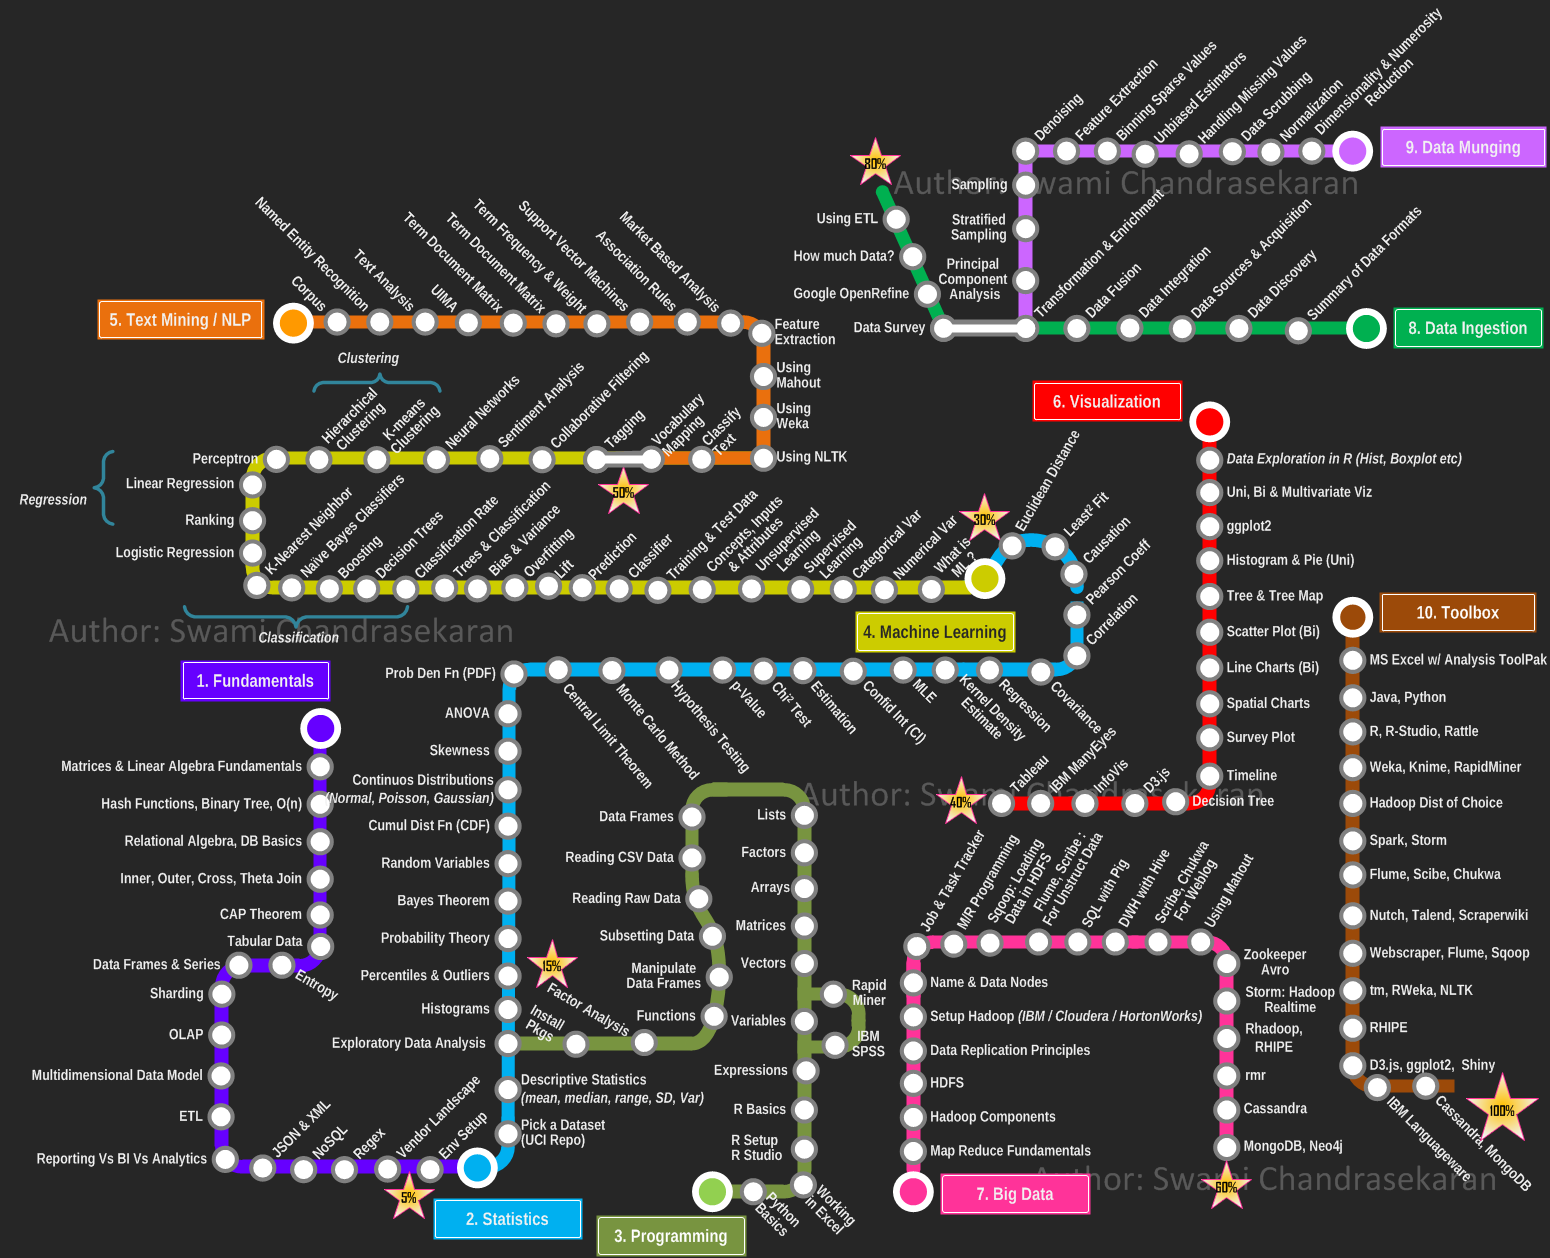
\includegraphics[width=\linewidth]{sections/images/RoadToDataScientist1.png}
    \caption{Road to Data Scientist}
    \label{RoadToDataScience}
\end{figure}


Comparison of \lstinline|R|, \lstinline|python|:focus on different aspects of `Statistics':
\begin{itemize}[topsep=2pt,itemsep=0pt]
    \item Differnece in programming philosophy: \lstinline|R| for data analysis and \lstinline|python| for data processing
    \item Difference in operating domain: \lstinline|R| for statistical programming while \lstinline|python| for general programming.
\end{itemize}



\subsection{Basic R. Manipulation}


\subsubsection{Installation and Maintenance of R.}
\begin{point}
    \textbf{Installing and Updating} 
\end{point}

\noindent  \lstinline|R.|: update by delete old version and install new version.
\begin{itemize}[topsep=2pt,itemsep=0pt]
    \item In CRAN (The Comprehensive \lstinline|R| Archive Network):\index{CRAN (The Comprehensive R Archive Network)} \url{https://cran.r-project.org}
    \item In Mirror@TUNA: \url{https://mirrors.tuna.tsinghua.edu.cn/CRAN}
\end{itemize}

\noindent RStudio: \url{https://www.rstudio.com}


\begin{point}
    \textbf{Running}  \lstinline|R.| \textbf{command} :
\end{point}

\begin{itemize}[topsep=2pt,itemsep=0pt]
    \item In \lstinline|R.| GUI\index{GUI (Graphical User Interface)};
    \item In \lstinline|R.| command line terminal;
    \item \lstinline|R. CMD BATCH|;
    \item \lstinline|Rscript|;
        \begin{itemize}[topsep=2pt,itemsep=0pt]
        \item Use \lstinline|>| to redirect output(overwrite);
        \item Use \lstinline|>>| to append output.
        \end{itemize}
\end{itemize}



\begin{point}
    \lstinline|R.| \textbf{package library}: packages are collection of \lstinline|R.| functions (as well as test data and sample code).
\end{point}

\begin{itemize}[topsep=2pt,itemsep=0pt]
    \item \lstinline|.libPaths()| show package library location\footnote{Unlike in \lstinline|C| or \lstinline|python| where \lstinline|.| is an operator, \lstinline|.| in \lstinline|R.| is just a common character, without special meaning.
    
    This feature can be used in naming self-defined functions: use \lstinline|.FUN_NAME1| for within-project function while \lstinline|FUN_NAME2| for external interface.} ;
    \item \lstinline|library('PACKAGE_NAME1','PACKAGE_NAME2',...)| load packages.
    \item \lstinline|install.packages('PACKAGE_NAME1','PACKAGE_NAME2',...)| install package from CRAN/mirrors;
    \item \lstinline|installed.packages()| show all installed packages;
    \item \lstinline|updata.packages(checkBuilt = TRUE, ask = FALSE)| update installed packages;
\end{itemize}

\begin{point}
    \textbf{Working directory}  manipulation:
\end{point}

\begin{itemize}[topsep=2pt,itemsep=0pt]
    \item \lstinline|getwd()| get current working directory;
    \item \lstinline|setwd('TARGET_PATH')| set working directory (as an existing path).
    \item \lstinline|dir()| show current directory.
\end{itemize}

\begin{point}
    Recommended \lstinline|R.| \textbf{Project Organization} : working directory organized like
\end{point}

\begin{itemize}[topsep=2pt,itemsep=0pt]
    \item \lstinline|data/| folder for structured original dataset;
    \item \lstinline|result/| folder for output result;
    \item \lstinline|presentation/| folder for result representing slides/reports/etc.;
    \item \lstinline|.r| project file $ \times n $.
\end{itemize}

\begin{point}
    Looking for \textbf{Help/Example}  of function:
\end{point}

\begin{itemize}[topsep=2pt,itemsep=0pt]
    \item \lstinline|?FUN_NAME()|;
    \item \lstinline|help('FUN_NAME')|;
\end{itemize}

\subsubsection{Data Structure and Basic Manipulation in R.}

\begin{point}
    Atomic Classes
\end{point}
\begin{itemize}[topsep=2pt,itemsep=0pt]
    \item \lstinline|'abc'| Character;
    \item \lstinline|3L| Integer;
    \item \lstinline|2.4| Numeric;
    \item \lstinline|TRUE,FALSE,T,F| Logical;
    \item Special types: \lstinline|NA|, \lstinline|NaN|, \lstinline|NULL|, \lstinline|Inf|
\end{itemize}

\begin{point}
    Operators
\end{point}
\begin{itemize}[topsep=2pt,itemsep=0pt]
    \item Numerical Operators: \lstinline|+|, \lstinline|-|, \lstinline|*|(multiply by column), \lstinline|/|, \lstinline|%*%|(matrix multiply), \lstinline|^|, \lstinline|%%|(remainder operate);
    \item Logical Operators: \lstinline|==|,etc.; \lstinline|&| and \lstinline{|} for common operator, \lstinline|&&| and \lstinline{||} for comparing the first element;
    \item Round a numeric:
    \begin{itemize}[topsep=2pt,itemsep=0pt]
        \item \lstinline|as.integer()|, round towards 0
        \item \lstinline|trunc()|
        \item \lstinline|ceiling()|
        \item \lstinline|floor()|
        \item \lstinline|round(NUMBER_TO_ROUND,digits = DIGITS)|
    \end{itemize}
\end{itemize}

\begin{point}
    Type Conversion
\end{point}

\begin{itemize}[topsep=2pt,itemsep=0pt]
    \item First need to meet the need of 
\end{itemize}

    
    Key Criterion: when converting mixed type in to the same type, use the type with more compatibility.
\begin{itemize}[topsep=2pt,itemsep=0pt]
    \item Logical $ \to $ Numeric: 
\end{itemize}

    

\begin{point}
    Data Structure
\end{point}
\begin{itemize}[topsep=2pt,itemsep=0pt]
    \item \textbf{Atomic Vector} : Column vector is the \textbf{basic} data structure in \lstinline|R.| (scalar is length=1 vector).
    
    Only data of the same class can be held in one vector.
    
    Initialization:
    \begin{itemize}[topsep=2pt,itemsep=0pt]
        \item Ordinary way: 
        \begin{itemize}[topsep=2pt,itemsep=0pt]
            \item \lstinline|c(1,2,3)|, \lstinline|c(T,FALSE,TRUE)|, \lstinline|c('a',NA,'b')|
            \item \lstinline|vector(mode = MODE,length = LENGTH)|
            \item \lstinline|logical(LENGTH)| return \lstinline|FALSE| vector 
        \end{itemize}
        
        where \lstinline|c()| for `combine'; 
        
        \lstinline|c()| combines all things into one vector, e.g. \lstinline|c(c(1,2,3),c(1,2))=(1,2,3,4,5)|.
        \item Sequence vector: 
        \begin{itemize}[topsep=2pt,itemsep=0pt]
            \item \lstinline|1:3.5=c(1,2,3)|, \lstinline|3:1=c(3,2,1)|
            \item \lstinline|seq(from, to ,by, length.out)|, \lstinline|length.out| for total vector length;
            \item \lstinline|rep(SEQ_TO_REP, times, lenght.out ,each)|, used in $ k $-fold cross validation labelling.
        \end{itemize}
    \end{itemize}
    
    Operations:
    \begin{itemize}[topsep=2pt,itemsep=0pt]
        \item between vectors of different length \lstinline|SHORT| and \lstinline|LONG|: First \lstinline|SHORT <- rep(SHORT,|\\\lstinline| length.out=length(LONG))|. Then operate \lstinline|SHORT| and \lstinline|LONG|.
        \item Element access: \lstinline|a[i]|
    \end{itemize}
    
         
    \fbox{
        \begin{minipage}{0.9\linewidth}

    \textbf{Vectorized Operation}: All operation in \lstinline|R.| are based on vector, and vectorized operation is Parallel Arithmetic, which is \textbf{much faster} than loop such as \lstinline|for| $ \longrightarrow $ Consider using vectorized opertion when writing code for \textbf{Speed}! Detail see \autoref{SubSubSectionVectorizedOperation}.
        \end{minipage}
    }

    \item \textbf{Factor} : A special kind of `vector' in \lstinline|R.|, used to label discrete categorical data.\footnote{Factor vector is stored as integer vector.}
    
    Initialization:

    \lstinline|factor(FACTOR_SEQ, levels = FACTOR_LEVEL, labels = ...)|, \lstinline|FACTOR_LEVEL| is the `rank' of each factor, \lstinline|labels| is the `tag' of levels. 

    A quick way to factorize a numeric vector \lstinline|x| by interval division:
    
    \lstinline|cut_number(x, NUM_OF_LEVELS)|

    \item \textbf{Matrix} : Only data of the same class can be held in one matrix.
    
    Initilaization:
    
    \lstinline|matrix(DATA_SEQ, nrow, ncol, byrow = FALSE, dimnames = NULL)|
    
    If \lstinline|length(DATA_SEQ) < nrow*ncol|, then \lstinline|DATA_SEQ| is repeated with \lstinline|length.out=nrow*ncol|. 
    
    Default: fill by column (because matrix is stored by column).

    Operation:
    \begin{itemize}[topsep=2pt,itemsep=0pt]
        \item Common operators \lstinline|+-*/^| etc. operate in column-by-column mode (vectorized operation).
        \item Binding matrix: \lstinline|cbind| for \lstinline|[A,B]| and \lstinline|rbind| for \lstinline|[A;B]|
        \item Transpose: \lstinline|t()|
        \item Matrix multiplication: \lstinline|%*%|
        \item Inverse matrix: \lstinline|solve()| (The essence of inversion is solving linear equations)
        \item Diagonal matrix:
        \begin{itemize}[topsep=2pt,itemsep=0pt]
            \item \lstinline|diag(VECTOR)| returns a matrix $ \mathrm{diag}\{ $\lstinline|VECTOR|$ \} $
            \item \lstinline|diag(MATRIX)| returns the diagonal element vector
        \end{itemize}
        \item Element access: \lstinline|a[i,j]|, \lstinline|a$OBJECT_NAME|
        \item Dimension: \lstinline|dim()|, \lstinline|nrow()|, \lstinline|ncol()|
        \item Rank: \lstinline|qr(MATRIX)$rank|
        % \item 
    \end{itemize}
    
    \item \textbf{List} : A pack containing various datatype, generally also a kind of vector(but not atomic vector)
    
    Initialization: \lstinline|list(OBJECT1,OBJECT2,...)|

    Element access: \lstinline|a[[i]]|
    \item \lstinline|data.frame|: `Mixture' of matrix and list. \lstinline|data.frame| is actually a kind of list(with some constraint), organized in the shape of matrix (but allowing different datatype for different columns, each column is a list object).
    
    Each column of \lstinline|data.frame| has name: \lstinline|names(DATA_FRAME)|, \lstinline|colnames(DATA_FRAME)|

    Element access: \lstinline|a[i,j]|, \lstinline|a[[i]]|, \lstinline|a$COL_NAME|
\end{itemize}

    
\begin{point}
    Data Read \& Write
\end{point}
\begin{itemize}[topsep=2pt,itemsep=0pt]
    \item Common R\&W: \lstinline|read.|/\lstinline|write.|
    \begin{itemize}[topsep=2pt,itemsep=0pt]
        \item \lstinline|read.table(FILE_NAME,header = FALSE,sep,colClasses,stringAsFactors = FALSE)|
        \item[${\color{red}\star }$] \lstinline|read.csv()| basically the same as \lstinline|read.table|
        \item[${\color{red}\star }$] \lstinline|write.table(DF,FILE_NAME,sep,row.names=FALSE)|
        \item \lstinline|readxl::read_xlsx(FILE_NAME,sheet = SHEET_NUM,range = 'RANGE')|
    \end{itemize}

    Some relative arguments:
    \begin{itemize}[topsep=2pt,itemsep=0pt]
        \item \lstinline|quote="'"|, use \lstinline|'| to quote/identify string, set \lstinline|quote=''| to avoid misread strings such as `Levene's Test'
        \item \lstinline|encoding='UTF-8'|, char encoding system, used especially for dataset containing CJK char.
        \item \lstinline|nrows=LINE_NUM| read first \lstinline|LINE_NUM| lines
        % \item 
    \end{itemize}

    \item Large Data Read \& Write: 
    \begin{itemize}[topsep=2pt,itemsep=0pt]
        \item preset \lstinline|colClasses|
        
\begin{lstlisting}[language=R]
temp.dat <- read.table(FILE_NAME, nrows = 100)
classes <- sapply(temp.dat, class)
dat <- read.table(FILE_NAME, colClasses = classes)
\end{lstlisting}
        \item \lstinline|readr::read_delim(FILE_NAME,delim=SEP)| can speed up
    \end{itemize}
    
    \item Text Write: \lstinline|sink(FILE_NAME,append=FALSE)|, write output into a file, the same as \lstinline|>| in terminal.
    \item \lstinline|.RData| Binary Format Read \& Write: RW in \lstinline|.RData| format, fast to load.
    \begin{itemize}[topsep=2pt,itemsep=0pt]
        \item \lstinline|save(DF,file = FILENAME)|
        \item \lstinline|load(FILE_NAME)|
    \end{itemize}
\end{itemize}

    




\subsubsection{Functions and Control Flow}
\begin{point}
    Program Speed:
\end{point}

\lstinline|system.time({COMMAND})|

\begin{point}
    Function Call
\end{point}
\begin{itemize}[topsep=2pt,itemsep=0pt]
    \item \lstinline|FUN_NAME(ARGUs)|
    \item \lstinline|do.call('FUN_NAME',LIST_OF_ARGUs)|, look for a function naming \lstinline|FUN_NAME| in \lstinline|R.| and call. 
    \item \lstinline|a % NEW_OPRTR % b| to call self-defined binary operator.
    \item \lstinline|'*'| etc. used in \lstinline|apply(FUN = '*')|
    \item \lstinline|R.| allows auto-completion to \lstinline|ARGUs|, e.g. \lstinline|rep(0,length.out=10)| = \lstinline|rep(0,length=0)|
\end{itemize}


\begin{point}
    Function Definition
\end{point}

\begin{rcode}
    Basic function definition in \lstinline|R.|
\begin{lstlisting}[language=R]
FUNC_NAME <- function(ARG1 = ARG1_DEF_VALUE , ARG2, ...) {
    FUNCTION_BODY
}
\end{lstlisting}
\end{rcode}

More key elements in \lstinline|funtion{}|
\begin{itemize}[topsep=2pt,itemsep=0pt]
    \item \lstinline|return(RETURN_OBJ)| at the end of function, without \lstinline|return()|, output the last line
    \item \lstinline|stopifnot(COND1,COND2,...)| at the beginning of function, used to test \lstinline|ARG| class
    \item \lstinline|stop(ERROR_MESG)| output error message
    \item \lstinline|...| as a special argument
    \begin{itemize}[topsep=2pt,itemsep=0pt]
        \item Pass \lstinline|...| to another func in this function
        \item Handle arbitrary number of input
    \end{itemize}
    \item Function can be defined within function
    \item Function is a kind of variable $ \longrightarrow $ used in \lstinline|apply|, \lstinline|sapply| etc. for vectorized programming.
    \item Anonymous function: used in \lstinline|sapply(X,FUN=function(){STATs})| for quick definition
    \item \lstinline|FUNC_NAME| can be used for new-defined binary operator as \lstinline|'%NEW_OPRTR%' <- function()|
\end{itemize}


\begin{point}
    Flow Control
\end{point}

\begin{itemize}[topsep=2pt,itemsep=0pt]
    \item \lstinline|if| and \lstinline|else if|, example:
\begin{lstlisting}[language=R]
if(COND1) {
    STATEMENT
} else if(COND2) {
    STATEMENT
} else {
    STATEMENT
}
\end{lstlisting}
    \item \lstinline|ifelse(COND,IF_YES_STAT,IF_NO_STAT)| a vectorized version of \lstinline|for+if else|.

    \item \lstinline|for|: Loop in \lstinline|R.| is \textbf{Extremely Slow}, avoid loop, use \textbf{vectorized operation}.  
\begin{lstlisting}[language=R]
for(VAR in SEQ) {
    STATEMENT
}
\end{lstlisting}
    \item \lstinline|switch(TEST_EXPR,CASE1 = RETN1,CASE2 = RETN2,...)|
 
    
        
    

\end{itemize}







\subsubsection{Vectorized Operation}\label{SubSubSectionVectorizedOperation}
\begin{itemize}[topsep=2pt,itemsep=0pt]
    \item \lstinline|apply()| function series:
\begin{itemize}[topsep=2pt,itemsep=0pt]
    \item \lstinline|apply(MAT,MARGIN,FUN)| for matrix apply, \lstinline|MARGIN=1| for each row, \lstinline|2| for each column
    \item \lstinline|lapply(LIST,FUN)| for list/\lstinline|data.frame|, apply \lstinline|FUN| on each list elements,\lstinline|list| returned
    \item[$ \color{red}\star $] \lstinline|sapply(X,FUN)| for list/\lstinline|data.frame| apply+simplify, \lstinline|vector/matrix/list| returned
    \item \lstinline|tapply(X,INDEX,FUN)|: for each index, use \lstinline|FUN| respectively.
    \item \lstinline|mapply(FUN,ARGU_OF_FUN)|, use argument name to label \lstinline|ARGU_OF_FUN|, or causes bad readability. 
    
    Example:
\begin{lstlisting}[language=R]
mapply(function(x,y,z,k){(x+k)^(y+z)} , x = ,y = ,z = ,k = )
\end{lstlisting}
    \end{itemize}

    \item \lstinline|Vfunc <- Vectorize(FUNC_NAME)|: define vectorize version of function.
    \item \lstinline|with()| and \lstinline|within()|:
    \begin{itemize}[topsep=2pt,itemsep=0pt]
         \item \lstinline|with(DF,aggregate(PART,by,FUN))|
        \item \lstinline|with(DF,STATE),within(DF,STATE)|,
     \lstinline|within| allows new column append
    \end{itemize}
    \item \lstinline|outer(VEC1,VEC2,FUN)|: A Two-variate extension of \lstinline|mapply()|, output wedge of two vectors.
    \item \lstinline|ifelse(COND,YES_STAT,NO_STAT)|, vectorization supported.
\end{itemize}





\subsubsection{Subsetting}
\begin{itemize}[topsep=2pt,itemsep=0pt]
    \item By position: \lstinline|x[RANGE]|
    \begin{itemize}[topsep=2pt,itemsep=0pt]
        \item \lstinline|x[4]|
        \item \lstinline|x[-4]|: without the $ 4^\mathrm{th} $ item (different from \lstinline|python|, where selects reciprocal $ \mathrm{4^{th}}  $ element).
        \item \lstinline|x[2:4]|
        \item \lstinline|x[c(1,2,5)]|
    \end{itemize}
    \item By name: \lstinline|x[,'COL_NAMEs']|, \lstinline|x[,'COL_NAME1':'COL_NAME2']|
    \item By condition: basically, \lstinline|x[LOGI_VEC]|
    \begin{itemize}[topsep=2pt,itemsep=0pt]
        \item \lstinline|x[x==10]|
        \item \lstinline|x[x %in% c(1,3,4)]|, linear search, not based on hash algorithm\footnote{If really needed, use \lstinline|env()| to reset environment.}.
    \end{itemize}

    Usually used for conditional selection of \lstinline|data.frame|
    \item Subsetting for \lstinline|data.frame| and list: \lstinline|x[[RANGE]]|


    Simplified/Preserved subsetting: whether preserved datatype, e.g. df $ \to $ df (preserved) v.s. df $ \to $ vector (simplified).
\begin{table}[H]
    \centering
    \renewcommand\arraystretch{1.15}
    \begin{tabular}{lll}
        \hline
        DataType&Simplified&Preserved\\
        \hline
        vector&\multicolumn{2}{c}{\lstinline|x[[1]]]| / \lstinline|x[1]|}\\
        list&\lstinline|x[[1]]|&\lstinline|x[1]|\\
        factor&\lstinline|x[1:4,drop=T]|&\lstinline|x[1:4]|\\
        matrix&\lstinline|x[,1]|&\lstinline|x[,1,drop=F]|\\
        \lstinline|data.frame|&\lstinline|x[,1]|,\lstinline|x[[1]]|&\lstinline|x[,1,drop=F]|,\lstinline|x[1]|\\
        \hline
    \end{tabular}
    \caption{Simplified/Preserved subsetting}
\end{table}
    \item Other subsetting:
    \begin{itemize}[topsep=2pt,itemsep=0pt]
        \item \lstinline|%in%| 
        \item \lstinline|unique()|, return with each element appears only one times
        \item \lstinline|duplicated()|, \lstinline|TRUE| when appear the $ n>1 $ times
        \item \lstinline|which(x==4)|, return position of matched element
        \item \lstinline|which.min()|, \lstinline|which.max|, \lstinline|min()|, \lstinline|max()|
        \item \lstinline|grep(REGEX,X,value)|, search for elements with \lstinline|REGEX| pattern: \lstinline|value=F| returns position, \lstinline|value=T| returns elements, \lstinline|grepl(REGEX,X)| returns logical vector
        \item \lstinline|match(TO_BE_MATCHED,TARGET)|, returns the index of elements of \lstinline|TO_BE_MATCHED| in \lstinline|TARGET|
        
        \begin{rcode}
            Example:
\begin{lstlisting}[language=R]
vec1 <- c('a','a','b','b','d','d','b')
vec2 <- c('d','a','b')
match(vec1,vec2)
> [1] 2 2 3 3 1 1 3
\end{lstlisting}
        \end{rcode}
        \item \lstinline|subset(X,...)|, \lstinline|...| a series of select criterion. \textbf{not} allowed: \lstinline|subset(X,...) <- | 
    \end{itemize}
    \item Use subsetting to sample: \lstinline|DATA[sample(1:nrow(DATA),NUM_OF_SAMPLE,replace),]|, \lstinline|replace=T| for with replacement
\end{itemize}

\subsubsection{Data Manipulation With dplyr. And tidyr.}
    \lstinline|dplyr| and \lstinline|tidyr| are two useful package for data cleaning \& manipulation. Use package \lstinline|tidyverse| include both of them.

    \lstinline|tidyverse| for \lstinline|tidy|uni\lstinline|verse|, includes \lstinline|dplyr|, \lstinline|tidyr|, \lstinline|readr|, \lstinline|ggplot2|, \lstinline|stringr|, etc.

\begin{point}
    \lstinline|%>%| pipe in \lstinline|tidyverse|: functions in \lstinline|tidyverse| use \lstinline|FUNC(DF,...)|, where \lstinline|DF| can be passed on by \lstinline|%>%|.

\end{point}


\begin{point}
    \lstinline|dplyr| Package. 
\end{point}

\begin{itemize}[topsep=2pt,itemsep=0pt]
    \item Cheet Sheet: \url{https://nyu-cdsc.github.io/learningr/assets/data-transformation.pdf}
    \item \lstinline|select(DF,...)|, where \lstinline|...| can use column index/name range as in subsetting, or some helper function for advanced subsetting:
    \begin{itemize}[topsep=2pt,itemsep=0pt]
        \item matching position:
        \begin{itemize}[topsep=2pt,itemsep=0pt]
            \item \lstinline|everything()|
            \item \lstinline|last_col()|
        \end{itemize}
        \item matching column name:
        \begin{itemize}[topsep=2pt,itemsep=0pt]
            \item \lstinline|start_with('PATTERN')|, \lstinline|end_with('PATTERN')|, \lstinline|contains('PATTERN')|
            \item \lstinline|match('REGEX')|, column name with \lstinline|REGEX| pattern
            \item \lstinline|num_range('x',1:4)| delect column name \lstinline|c('x1','x2','x3','x4')|
            \item \lstinline|any_of(CHR_VEC)| select column from \lstinline|CHR_VEC|
        \end{itemize}
        \item \lstinline|where(FUN)|, select those \lstinline|FUN(COL_NAME)| returns \lstinline|TRUE|
    \end{itemize}
    \item \lstinline|filter(DATA,CONDs)|, select elements with \lstinline|CONDs| conditions
    \item \lstinline|arrange(DATA,COL)|, sort by \lstinline|COL|, \lstinline|arrange(DATA,desc(COL))| for descending order
    \item \lstinline|mutate(DATA,...)|, append new columns according to \lstinline|...| definition; \lstinline|transmute()| drops original columns.
    
    \lstinline|...| definition can use advanced window function:
    \begin{itemize}[topsep=2pt,itemsep=0pt]
        \item \lstinline|lead(COL)|,\lstinline|lag(COL)|, e.g. \lstinline|lead(COL)[i]|=\lstinline|COL[i+1]|, can use \lstinline|...=COL-lead(COL)| for differnetial
        \item \lstinline|dense_rank(COL)|, \lstinline|percent_rank(COL)| rank number
        \item \lstinline|ntile(COL,N)| break into \lstinline|N| groups labeling \lstinline|1:N|
        \item \lstinline|cume_dist(COL)|, \lstinline|cummean(COL)|, \lstinline|cumsum(COL)|, \lstinline|cummax(COL)|, \lstinline|cummin(COL)|, etc. cumulative value
    \end{itemize}
    
    \item \lstinline|summarise(data,...)|, \lstinline|...| for summarise function.

    \item Row selection:
    \begin{itemize}[topsep=2pt,itemsep=0pt]
        \item \lstinline|slice(DF,ROW_RANGE)|
        \item \lstinline|distinct(DF)| remove duplicated rows
        \item \lstinline|sample_frac(DF,FRAC,replace)|, sample \lstinline|FRAC| fraction from \lstinline|DF|
        \item \lstinline|sample_n(DF,N,replace)|, sample \lstinline|N| cases from \lstinline|DF|
        \item \lstinline|top_n(DF,AMOUNT,RANK_COL)| select \lstinline|AMOUNT| top ranking by \lstinline|RANK_COL| cases
    \end{itemize}
    \item Data combining see slides.
\end{itemize}

\begin{point}
    \lstinline|tidyr| Package
\end{point}
\begin{itemize}[topsep=2pt,itemsep=0pt]
    \item Cheet Sheet: \url{https://leadousset.github.io/intro-to-R/cheatsheet_tidy.pdf}
    \item \lstinline|gather(DF,key='KEY_NAME',value='VALUE_NAME',...,na.rm)|, melt a \lstinline|data.frame|. 
    
    e.g. \lstinline|gather(df,'KEY','VALUE',c('COL1','COL2','COL3'))| transfers \lstinline|...| as:
    \[
        \begin{matrix}
            \text{ID}&\text{COL1}&\text{COL2}&\text{COL3}\\
            1&a_1&b_1&c_1\\
            2&a_2&b_2&c_2\\
            \vdots&\vdots&\vdots&\vdots
        \end{matrix}
        \quad\to\quad
        \begin{matrix}
            \text{ID}&\text{KEY}&\text{VALUE}\\
            1&\text{COL1}&a_1\\
            2&\text{COL1}&a_2\\
            \vdots&\vdots&\vdots\\
            1&\text{COL2}&b_1\\
            2&\text{COL2}&b_2\\
            \vdots&\vdots\\
            1&\text{COL3}&c_1\\
            2&\text{COL3}&c_2\\
            \vdots&\vdots
        \end{matrix}
    \]
    \item \lstinline|spread(DF,key='KEY_NAME',value='VALUE_NAME')|, inverse of \lstinline|gather()|
    \item \lstinline|separate(DF,COL,into=SET_VEC,sep='REGEX')|, separate \lstinline|COL| into columns with name in \lstinline|SET_VEC|, sep according to \lstinline|sep|
    \item \lstinline|unite(DF,COL,SET_VEC,sep='')| inverse of \lstinline|separate()|
\end{itemize}

    


\subsection{Text Processing \& Text Mining}
    \begin{itemize}[topsep=2pt,itemsep=0pt]
        \item Data cleaning
        \item Data manipulation
        \item Information extraction: mode identifying/relation extraction
        \item Text mining: anaylzing token distribution, ignore word order
        \item NLP: concept identifying based on sentence; untimate goal: `understand' sentence meaning.
    \end{itemize}
    
    Tools for Text processing:
\begin{itemize}[topsep=2pt,itemsep=0pt]
    \item \lstinline|R.|: suitable for easy task 
    \item \lstinline|python.|: best
    \item \lstinline|java|: strong, but not suitable for deep learning
    \item \lstinline|c++|: fast, inadequate package
    \item \lstinline|Notepad++|/\lstinline|Vim|
\end{itemize}

    
        



\subsubsection{Basic Text Manipulation With stringr.}
\begin{point}
    \lstinline|R. base| \& \lstinline|stringr| package:
\end{point}

    The prior one is used more often

\begin{itemize}[topsep=2pt,itemsep=0pt]
    \item Cheet Sheet: \url{http://edrub.in/CheatSheets/cheatSheetStringr.pdf}
    \item \lstinline|str_length(STRING)|, \lstinline|nchar(STRING)|
    \item \lstinline|paste(...,collapse=NULL)|,\lstinline|str_c(...)|, both are vectorized operation
    
    Argument:
    \begin{itemize}[topsep=2pt,itemsep=0pt]
        \item \lstinline|sep|: sep between each \lstinline|...| corresponding elements, with \lstinline|collapse=NULL|, return a char vector
        \item \lstinline|collapse|: sep when combining \lstinline|collapse=NULL| vector elements, \lstinline|NULL| for not combining
        \item Special character: \lstinline|\t| tab, \lstinline|\r| \& \lstinline|\n| \& \lstinline|\r\n| new line, \lstinline|\xad| `-' at end on line for word-connecting
    \end{itemize}
    
    \item \lstinline|str_split(STRING,pattern='REGEX')|/\lstinline|strsplit()|, split string at \lstinline|REGEX| pattern fitted, list returned
    \item \lstinline|str_sub(STRING,start,end)|, \lstinline|substr()|. The \lstinline|start| char to \lstinline|end| char of string, use negative index as in \lstinline|python|.
     
    Can be used to replace: \lstinline|str_sub(...) <- REP_STR|
    \item \lstinline|str_locate_all('STRING',pattern='REGEX')|/\lstinline|str_match_all('STRING',pattern='REGEX')|

    \lstinline|grep(pattern='REGEX',x='STRING',value=T)|, search for elements with \lstinline|REGEX| pattern: \lstinline|str_locate_all()| or \lstinline|value=F|  returns position, \lstinline|str_match_all()| or \lstinline|value=T| returns elements.
    
    \item \lstinline|str_replace_all('STRING',pattern='REGEX',replacement='REP')|
    \lstinline|grepl(REGEX,X)| returns logical vector, include or not.
    \lstinline|str_extract_all('STRING',pattern='REGEX')|
    \item \lstinline|gsub(pattern='REGEX',replacement='REP',x='STRING')|, replace \lstinline|REGEX| field with \lstinline|REP|
    % \item Extracting word: 
    \item \lstinline|str_trim(...,side = )|, trim extra white space at \lstinline|side='both'|/\lstinline|'left'|/\lstinline|'right'|
    % \item Padding: \lstinline|str_pad()| append space
\end{itemize}




\subsubsection{Regular Expression}
    Regular expression is a text pattern/mode. abbr. regex/regexp. Regex is supported in most common language, same syntax used.

    Tutorial: \url{https://www.runoob.com/regexp/regexp-tutorial.html}

\begin{point}
    Key Elements
\end{point}

\begin{itemize}[topsep=2pt,itemsep=0pt]
    \item Literal: common char, e.g. \lstinline|a|. Include most char on keyboard. Upper/Lower case sensitive.
    \item Metacharacters: \lstinline!\^$.|?*+()[]{}!, use e.g. \lstinline|\.| to escape meaning.
    
    Note: when typing regex in programming language, sometimes use \lstinline|\\.|: \lstinline|\\.| $ \xrightarrow[]{\text{language interpreter}}  $ \lstinline|\.| $ \xrightarrow[]{\text{regex interpreter}}  $ identifying \lstinline|.|

    \item Character Class: \lstinline|[]|, identify one of elements in \lstinline|[]|. \lstinline|^| within \lstinline|[]| for $ \complement $. 
    \begin{itemize}[topsep=2pt,itemsep=0pt]
        \item e.g. \lstinline|gr[ae]y| identifies \lstinline|grey| and \lstinline|gray|.
        \item e.g. \lstinline|[0-9]| numbers, \lstinline|[a-zA-z]| letter
        \item e.g. \lstinline|q[^x]| matches \lstinline|question|, not matchs \lstinline|qxestion|, not matches \lstinline|Iraq|
    \end{itemize}

    character class shorthand
\begin{table}[H]
    \centering
    \renewcommand\arraystretch{1.15}
    \begin{tabular}{lll}
        \hline
        ShortHand&Meaning&Equivalant \lstinline|REGEX|\\
        \hline
        \lstinline|\d|&numeric digit&\lstinline|[0-9]|\\
        \lstinline|\D|&Not numeric digit&\lstinline|[^\d]|\\
        \lstinline|\w|&a word character&\lstinline|[a-zA_Z0-9_]|\\
        \lstinline|\s|&white space&\lstinline|[\t\r\n\f]|\\
        \hline
    \end{tabular}
\end{table}

    \item Wildcard(通配符): \lstinline|.| matches any single character except line break \lstinline|\r|,\lstinline|\n|
    \item Anchor(词边界/定位符): match `word boundary' (not the space at the start/end of string).
    
    \lstinline|^| string start, \lstinline|$| string end, \lstinline|\b| word boundary, \lstinline|\B| not-a-word-boundary position
    \item Repetition/Quantifier: here \lstinline|X| for some regex pattern like \lstinline|CHAR|, \lstinline|[]| etc.
    
\begin{table}[H]
    \centering
    \renewcommand\arraystretch{1.15}
    \begin{tabularx}{0.9\linewidth}{XXXX}
        \hline
        Greedy&$ \color{red}\star $ Reluctant&Possessive&Freq of Occurrence\\
        \hline
        \lstinline|X?|&\lstinline|X??|&\lstinline|X?+|& $ 0,1 $\\
        \lstinline|X+|&\lstinline|X+?|&\lstinline|X++|& $ \geq 1 $\\
        \lstinline|X*|&\lstinline|X*?|&\lstinline|X*+|& 0,$ >1 $\\
        \lstinline|X{n}|&\lstinline|X{n}?|&\lstinline|X{n}+|& $ n $\\
        
        \lstinline|X{n,}|&\lstinline|X{n,}?|&\lstinline|X{n,}+|& $ \geq n $\\
        \lstinline|X{n,m}|&\lstinline|X{n,m}?|&\lstinline|X{n,m}+|& $ [n,m] \qquad\qquad  $\\
        \hline
    \end{tabularx}
\end{table}

    Example: Search `foo' in `xfooxxxxxxfoo':
    \begin{itemize}[topsep=2pt,itemsep=0pt]
        \item Greedy: `xfooxxxxxxfoo' found at index 0-13
        \item[$ \color{red}\star $] Reluctant: `xfoo' found at index 1-4, `xxxxxxfoo' found at index 4-13
        \item Possessive: no match found (not usually used)
    \end{itemize}
    
    Example: regex match 'aaaa'
    \begin{itemize}[topsep=2pt,itemsep=0pt]
        \item 
    \end{itemize}
    
        
    \item Alternation \& Grouping \& Back Reference: \lstinline!XA|XB! identify \lstinline|XA| or \lstinline|XB|, use grouping \lstinline|()| to set boundary of XA,XB.
    
    Use \lstinline|\n| for back reference the $ n^\mathrm{th}  $ group. 
\begin{rcode}
    Example: search for immediate repeat word in a sentence
\begin{lstlisting}[language=R]
(\b[a-zA-Z]+\b) \1
\end{lstlisting}
\end{rcode}
    \item Lookaround: 
    \begin{itemize}[topsep=2pt,itemsep=0pt]
        \item LookAhead: \lstinline|(?<=X)q|
        \item LookBehind: \lstinline|q(?=X)|
    \end{itemize}
    
        
\end{itemize}

    
\subsubsection{Web Scraping}
    Basic elements of web page:
\begin{itemize}[topsep=2pt,itemsep=0pt]
    \item HTML (HyperText Markup Language): structure and content of page
    \item CSS (Cascading Style Sheet): page style.
    \item JavaScript: functionality, interaction
\end{itemize}

        
Basic \lstinline|html| document format:
\begin{rcode}
\begin{lstlisting}[language=R]
<!DOCTYPE html> # an html document
<html> # html page begin
<head> # head elements declare
<meta charset="utf-8">
<title> TITLE OF WEB PAGE </title>
</head>
<body> # html body begin
 
<h1> HEADING 1 </h1>
<p class='TEST_TEXT'> PARAGRAPH 1 </p>
 
</body>
</html>
\end{lstlisting}
\end{rcode}

    We can use elements like \lstinline|<p>| or \lstinline|class| to extract page information.

\begin{point}
    Web Scraping with \lstinline|rvest.|
\end{point}

\begin{itemize}[topsep=2pt,itemsep=0pt]
    \item \lstinline|pge <- read_html('URL')|: page read
    
    Proxy set: \lstinline|Sys.setenv(https_proxy='http://127.0.0.1:7890')|
    \item \lstinline|pge %>% html_elements(css='.CSS_CLASS_NAME') %>% html_text()|: basic scraping. use SelectGadget tool for help finding proper css label.
\end{itemize}

% \subsubsection{Word Segmentation}



\subsection{Graphic in R.}

\subsubsection{R::base Plotting}

    Plot function in \lstinline|R::base|:\index{Plot Parameters in R.}
\begin{lstlisting}[language=R]
plot(X,Y) # scatter/line plot of Y-X
plot(FUNC_OBJ, from = , to = ) # function plot ranging in c(from, to)
plot(FACTOR) # barplot of factors
plot(FACTOR, Y) # boxplot of numeric v.s. levels of factor
plot(DATA.FRAME) # correlation plot
plot(ANY_PLOTTABLE_OBJ) # plot any plottable object 
\end{lstlisting}

\begin{itemize}[topsep=2pt,itemsep=0pt]
    \item Plot saving: first open a plotting device, then make plot and close the device
\begin{lstlisting}[language=R]
pdf("PLOT_FILE_NAME.pdf", FIG_HEIGHT, FIG_WIDTH)
plot(PLOT_PARAM)
dev.off()
\end{lstlisting}
    \item \lstinline|plot()| plotting parameters:
    \begin{itemize}[topsep=2pt,itemsep=0pt]
        \item \lstinline|main = | string for title; or use \lstinline|title('TITLE')| as the next command
        \item \lstinline|sub = | string for subtitle;
        \item \lstinline|xlab = , ylab = | string axis labels;
            \item adding \LaTeX expression as text: use \lstinline|main = expression(PLOTMATH_EXPRESSION)|, use \lstinline|?plotmath| to look for possible symbols
        \item \lstinline|xlim = , ylim = | axis range, e.g. use \lstinline|xlim = c(0,100)|
        \item \lstinline|type = | value taken in \lstinline|c('p', 'l', 'b', 'o', 's', 'h')| for plot \textbf{type}
        \begin{figure}[H]
            \centering
            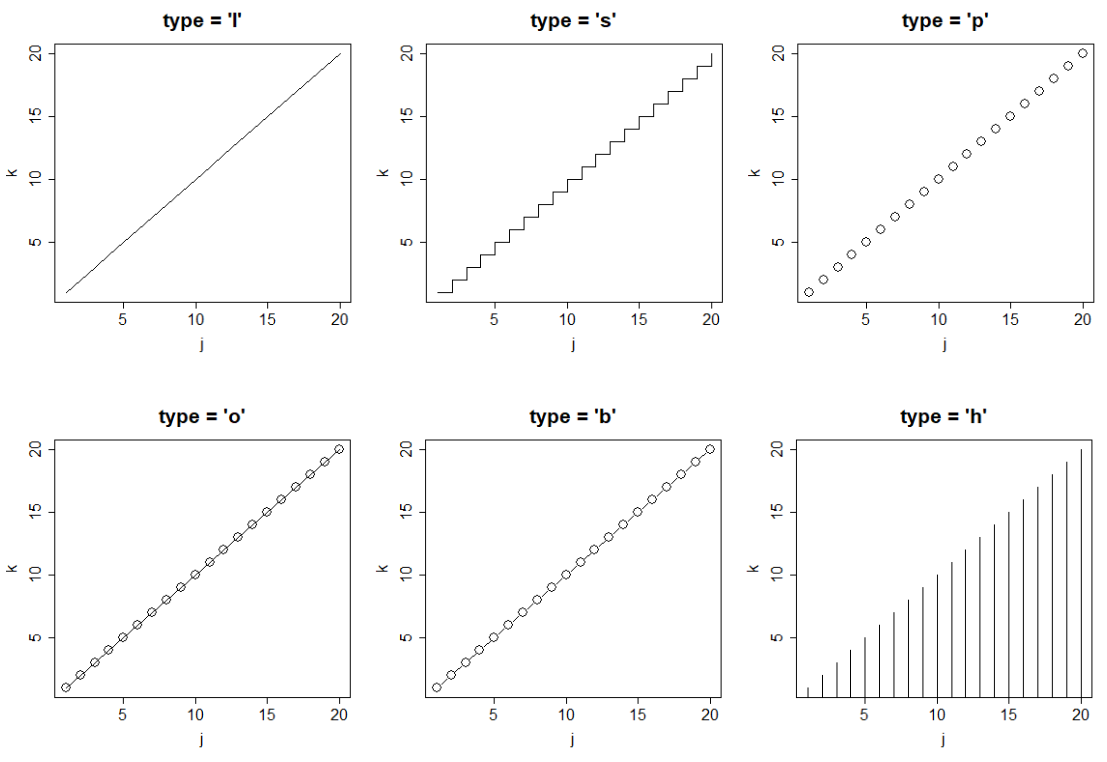
\includegraphics[width=0.8\linewidth]{sections/images/2022-08-18-11-24-35.png}

            \label{}
        \end{figure}
        
        \item \lstinline|pch = | \textbf{p}oint \textbf{ch}aracter, value taken in \lstinline|0:25| for defulat point charaters listed below, or use (vector of) charater to specify, e.g. \lstinline|pch = c('❄')|
        \begin{figure}[H]
            \centering
            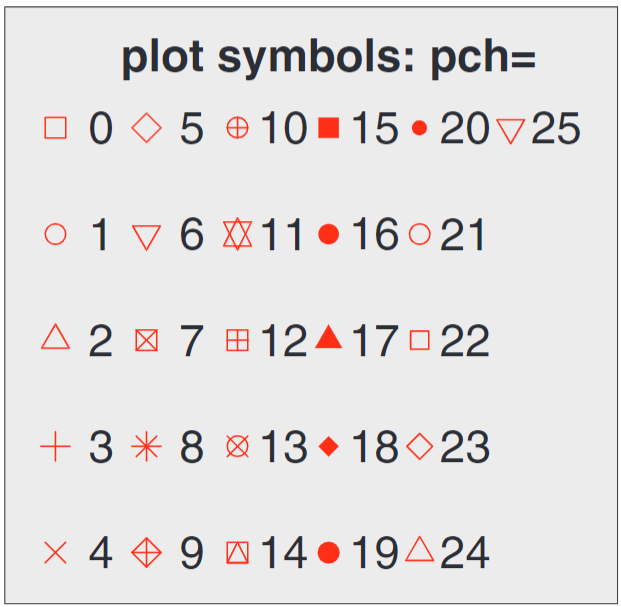
\includegraphics[width=0.3\linewidth]{sections/images/2022-08-18-11-14-15.png}

            \label{}
        \end{figure}

        \item \lstinline|lty = | \textbf{l}ine \textbf{ty}pe, value taken in \lstinline|1:6| (0 for not shown)
        \begin{figure}[H]
            \centering
            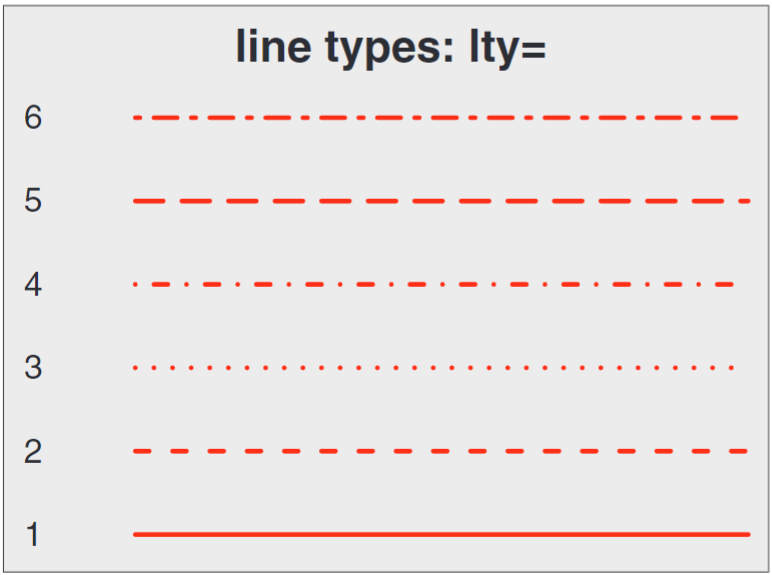
\includegraphics[width=0.4\linewidth]{sections/images/2022-08-18-11-15-34.png}

            \label{}
        \end{figure}

        \item \lstinline|cex = | \textbf{c}haracter \textbf{ex}pansion, relative size with 1 as baseline and default. 
        
        Some derivative function to control size of other plotting elements:
        \begin{itemize}[topsep=2pt,itemsep=0pt]
            \item \lstinline|cex.axis = | relative size of axis node text
            \item \lstinline|cex.lab = | relative size of labels
            \item \lstinline|cex.main = | relative size of title 
            \item \lstinline|cex.sub = | relative size of subtitle 
        \end{itemize}
        
        \item \lstinline|lwd = | \textbf{l}ine \textbf{w}i\textbf{d}th, relative width of line with 1 as baseline and default
        \item \lstinline|col = | \textbf{color} of elements in plot, value examples for color white:
        \begin{itemize}[topsep=2pt,itemsep=0pt]
            \item Index: \lstinline|col = 1| predefined color in \lstinline|R.| 
            \item Color name: \lstinline|col = 'white'|, use \lstinline|colors()| to see all available color names
            \item Hexadecimal code: \lstinline|col = '#FFFFFF'|
            \item RGB code: \lstinline|col = rgb(1,1,1)|, \lstinline|col = rgb(255,255,255, maxColorValue = 255)|
            \item HSV code: \lstinline|col = hsv(0,0,1)|
        \end{itemize}

        \lstinline|col = | can accept vector for various colors, or acccept some function for continuous colors:
        \begin{itemize}[topsep=2pt,itemsep=0pt]
            \item Discrete color: \lstinline|col = c('red','blue')|, or use \lstinline|col = df$GROUP| to color different groups
            \item Continuous color function: \lstinline|rainbow(NUM_OF_COLORS)|, \lstinline|heat_colors()|, \lstinline|terrain.colors()|, \lstinline|topo.colors()|, \lstinline|cm.colors()|
        \end{itemize}

        Some derivative function to control color of other plotting elements:
        \begin{itemize}[topsep=2pt,itemsep=0pt]
            \item \lstinline|col.axis = | color of axis node text
            \item \lstinline|col.lab = | color of labels
            \item \lstinline|col.main = | color of title 
            \item \lstinline|col.sub = | color of subtitle 
            \item \lstinline|bg = | color of background
        \end{itemize}

        \item \lstinline|font = | \textbf{font} used in plot, with 1 = plain, 2 = bold, 3 = italic,
        4 = bold italic

        Some derivative function to control font of other plotting elements:
        \begin{itemize}[topsep=2pt,itemsep=0pt]
            \item \lstinline|font.axis = | font of axis node text
            \item \lstinline|font.lab = | font of labels
            \item \lstinline|font.main = | font of title 
            \item \lstinline|font.sub = | font of subtitle 
            \item \lstinline|ps = | baseline font \textbf{p}oint \textbf{s}ize, i.e. text size = \lstinline|ps*cex|
            \item \lstinline|family = | extra text type, value taken in \lstinline|c('serif', 'sans', 'mono')|m etc. use \lstinline|names(pdfFonts())| to see possible font families
        \end{itemize}
        \item \lstinline|bty = | \textbf{b}ox \textbf{ty}pe of the box surrounding the figure. Value taken in \lstinline|c('o', '7', 'L', 'U', 'C', 'n')| 
    \end{itemize}
    \item \lstinline|axis()| parameters for axis settings: after using \lstinline|xaxt = 'n'| or \lstinline|yaxt = 'n'| to remove correponding axis when executing \lstinline|plot()|, other variation of axis could be made by using \lstinline|axis()|
    \begin{itemize}[topsep=2pt,itemsep=0pt]
        \item \lstinline|axis(1)| for creating $ x $ aixs, \lstinline|axis(2)| for creating $ y $ aixs. Here we would use $ x $ axis in the following parts.
        \item \lstinline|aixs(1, at = )| to specify ticks.
        \item \lstinline|plot(las = )| to specify rotation of ticks, value taken in \lstinline|c('Parallel', 'Horizontal', 'Perpendicular', 'Vertical')|
        \item \lstinline|plot(xlim = c( , ), ylim = c( , ))| for axis limits
        \item \lstinline|plot(log = )| for log transfrom on axis, value taken in \lstinline|c('x', 'y', 'xy')|. 
    \end{itemize}
    
        

    \item \lstinline|legend()| parameters:
    \begin{itemize}[topsep=2pt,itemsep=0pt]
        \item \lstinline|x = | position of legend, value taken in \lstinline|c("top", "bottom", "topleft", "topright", "bottomleft", "bottomright")|
        \item \lstinline|inset = |
        \item other parameters are set following the setting in \lstinline|plot|. An example:
\begin{lstlisting}[language=R]
legend("bottomright", legend = c("red", "green"), lty = c(2,4), lwd = 3, col = c("red", "green"))
\end{lstlisting}

    \end{itemize}

    \item \lstinline|text(X_COOR, Y_COOR, labels = TEXT)| parameters for adding text in figure. An application is \lstinline|text(df$X, df$Y, labels = df$Z)| to label each point.
    \begin{itemize}[topsep=2pt,itemsep=0pt]
        \item \lstinline|pos = | \textbf{pos}ition of text around the coordinate point, value taken in \lstinline|c(1,2,3,4)| 
    \end{itemize}
    
    \item \lstinline|lines()| to put an extra line on existing figure (device). Parameters are similarly set as \lstinline|plot()|
    
    \item \lstinline|par()| to set global \textbf{par}ameters. An example to put 3 different figure in the same device:
\begin{lstlisting}[language=R]
opar <- par(no.readonly = TRUE) # copy original setting
par(mfrow = c(1,3))
plot()
plot()
plot()
par(opar)
\end{lstlisting}

\end{itemize}

\begin{point}
    More Charts
\end{point}

\begin{itemize}[topsep=2pt,itemsep=0pt]
    \item \lstinline|barplot(counts, horiz, besides, ...)| for bar plot. Data should be first prepared by \lstinline|counts <- table(Y_TO_COUNT)|. 
    \item \lstinline|hist(x, breaks, freq, ...)| for histogram.
    \item \lstinline|plot(density(df, kernel = ), ...)| for density plot.
    \item \lstinline|boxplot(x, ...)| for box plot. use \lstinline|boxplot(x ~ GROUP, data = , ...)| to plot grouped boxplot
    \item \lstinline|dotchart(x, labels, groups, ...)| to compare \lstinline|x| value for categories
\end{itemize}


\subsubsection{R::ggplot2 Plotting}
    \lstinline|ggplot2|: \textbf{G}rammar of \textbf{G}raphics \textbf{plot} (2nd edi). It provides a convenient way to produce fancy plots. Reference see \url{https://ggplot2.tidyverse.org/reference/}\index{ggplot2}
    
    Basic steps for \lstinline|ggplot2|:
    \begin{enumerate}[topsep=2pt,itemsep=2pt]
        \item Specify data and arsthetic mapping
        \item Adding 'layers' with \lstinline|geom_|
        \item Adding labels
    \end{enumerate}

    An example:
\begin{lstlisting}[language=R]
ggplot(data=mtcars, aes(x=wt, y=mpg)) +
    geom_point(pch=17, color="blue", size=2) +
    geom_smooth(method="lm", color="red", linetype=2) +
    labs(title="Automobile Data", x="Weight", y="Miles Per Gallon")
\end{lstlisting}


    Elements in \lstinline|ggplot2|:
    \begin{itemize}[topsep=2pt,itemsep=0pt]
        \item \lstinline|aes()| to specify \textbf{aes}thetic mapping, e.g. \lstinline|aes(x = , y = , col = , ...)|. Used in \lstinline|ggplot()| as global setting, in \lstinline|geom_()| as local override (different \lstinline|geom_()| may need different local settings). Examples:
\begin{lstlisting}[language=R]
aes(x = mpg ^ 2, y = wt / cyl, col = am)
#> Aesthetic mapping: 
#> * x -> mpg^2
#> * y -> wt/cyl
#> * color -> am
\end{lstlisting}

        \item \lstinline|geom_| layer to specify statistical figure you want. Some useful plot:
\begin{table}[H]
    \centering
    \renewcommand\arraystretch{1.15}
    \begin{tabularx}{0.9\linewidth}{XXp{0.5\linewidth}}
        \hline
        \hline
        \lstinline|geom_()| Function    &Charts         &Options\\
        \hline
        \lstinline|geom_bar()|          &bar plot       &\lstinline|color, fill, alpha|\\
        \lstinline|geom_boxplot()|      &box plot       &\lstinline|color, fill, alpha, notch, width|\\
        \lstinline|geom_density|        &density plot   &\lstinline|color, fill, alpha, linetype|\\
        \lstinline|geom_histogram()|    &histogram      &\lstinline|color, fill, alpha, linetype, binwidth|\\
        \lstinline|geom_hline()|        &horizontal line            &\lstinline|color, alpha, linetype, size|\\
        \lstinline|geom_vline()|        &vertical line            &\lstinline|color, alpha, linetype, size|\\
        \lstinline|geom_line()|         &line gragh     &\lstinline|color, alpha, linetypem size|\\
        \lstinline|geom_point()|        &scatter plot       &\lstinline|color, alpha, shape, size|\\
        \lstinline|geom_smooth()|       &fitted line        &\lstinline|method, formula, color, fill, linetype, size|\\
        \lstinline|geom_violin()|       &violin plot        &\lstinline|color, fill, alpha, linetype|\\
        \lstinline|geom_text()|     &text annotation        &see functon help\\
        \hline
        \hline
    \end{tabularx}
\end{table}
        \item \lstinline|labs(title, x, y)| to specify labels and title
        \item \lstinline|facet_grid()| and \lstinline|facet_wrap()| to plot multiple plot, with factor levels as categories, parameters:
        \begin{itemize}[topsep=2pt,itemsep=0pt]
            \item \lstinline|facets = | facet variable. For \lstinline|facet_wrap()| use \lstinline|~VAR1| (one variable); \lstinline|facet_grid()| use \lstinline|.~VAR1| or \lstinline|VAR1~.| or \lstinline|VAR1~VAR2| (allow two variable)
            \item \lstinline|nrow = , ncol = | grid shape
            \item \lstinline|shrink = | whether adjust ticks, set \lstinline|TRUE| or \lstinline|FALSE|
            \item \lstinline|drop = | whether drop levels with censored data, set \lstinline|TRUE| or \lstinline|FALSE|
        \end{itemize}
        \item \lstinline|theme()| to set fonts, backgrouds, gridlines, etc. 
        
        There are some pre-defined theme: \lstinline|theme_grey(), theme_bw(), theme_linedraw(), theme_light(), theme_dark(), theme_minimal(), theme_classic(), theme_void(), theme_test()|.
        
        
        Detailed elements in a plot is adjust by passing \lstinline|element_()|:
        \begin{itemize}[topsep=2pt,itemsep=0pt]
            \item \lstinline|element_line()| set some line element
            \item \lstinline|element_rect()| set some rectangular element
            \item \lstinline|element_text()| set some text element
        \end{itemize}
        
        Some useful command:
        \begin{itemize}[topsep=2pt,itemsep=0pt]
            \item \lstinline|plot.title = element_text(hjust = 0.5)| adjust position of title to mid. Other similar parameters: \lstinline|plot.background, plot.title.position, plot.subtitle, plot.caption, plot.caption.position, plot.tag, plot.tag.position, plot.margin|
            \item \lstinline|panel.background = element_rect(fill = 'white', color = 'blue')| adjust figure background and border. Other similar parameters: \lstinline|panel.grid.major/minor.x/y|
            \item \lstinline|aspect.ratio = | height:width
            \item \lstinline|legend.position = 'none'| to remove automatic legend
        \end{itemize}
        
            
        
            
        
            
        \item \lstinline|ggsave('FILE_NAME', PLOT, WID, HEI)|, or use \lstinline|ggsave('FILE_NAME')| to save the active device.
    \end{itemize}
    
        
    
        



    



\newpage

\section{统计计算与软件部分}\label{SecStatisticalComputingAndSoftware}
\begin{center}
    Instructor: Zaiying Zhou
\end{center}

\subsection{Algorithm Theory Introduction}

% \subsubsection{Float Storage}

\subsubsection{Finite Precision Computation}
    An arbitrary real number $ r\in\mathbb{R} $ is represented as (the nearest adjacent) float number $ v_r $. A float is basically stored as (example take 32-bit float): 1 bit \textbf{S}ign + 8 bit \textbf{E}xponent + 23 bit \textbf{M}antissa.
\begin{equation}\label{EqaNormalizedFloat}
    v=(-1)^S\times 2^{E-127}\times \left(1+\sum_{i=1}^{23}(M_i\times 2^{-i})\right)
\end{equation}
    
    
    Further, extreme value of $ (M,E) $ is used for some `special value': denormalized number, NaN, inf, etc. 
\begin{itemize}[topsep=2pt,itemsep=0pt]
    \item Denormalized number: to fill the gap $ [0,\pm 2^{-126}] $($ E=1 $), for $ E=0 $ extremely small number, definition use\index{Normalized Number} 
    \begin{align}
        v_\mathrm{denormalized}=(-1)^S\times 2^{1-127}\times \left({\color{red}0}+\sum_{i=1}^{23}(M_i\times 2^{-i})\right)  
    \end{align}
    i.e. for $ E=0 $, range $ [2^{-127},2^{-126})_\mathrm{nor}\to [0,2^{-126})_\mathrm{denor} $.
    \item NaN: $ (E=255,M\neq 0) $
    \item inf: $ (E=255,M=0) $
\end{itemize}

\begin{table}[H]
    \centering
    \renewcommand\arraystretch{1.15}
    \begin{tabular}{clll}
        \hline
        &$ E=0 $&$ 0<E<E_{\mathrm{max} } $&$ E=E_{\mathrm{max} }  $\\
        \hline
        $ M=0 $&$ \pm 0 $&\multirow{2}{*}{$  v_\mathrm{normalized} $}&$ \pm\infty $\\
        $ M\neq 0 $&$  v_\mathrm{denormalized} $&&NaN\\
        \hline
    \end{tabular}
    \caption{Normalized Number}
    \label{}
\end{table}

    


    Use $ v_r $ to represent $ r $: approximation $ r\sim v_r $, the round-off error of $ r $:
\begin{itemize}[topsep=2pt,itemsep=0pt]
    \item Absolute rounding error: 
    \begin{align}
         \varepsilon =|r-v_r|
    \end{align}
    \item Relative rounding error:
    \begin{align}
        \varepsilon _\mathrm{machine}=\dfrac{|r-v_r|}{|r|}  =\mathrm{const}
    \end{align}
\end{itemize}
    Note that for large $ |r| $, the adjacency between floats $ |r-v_r|=|r|\varepsilon _\mathrm{machine}  $ might be large, even cause some integer missing.   

\begin{point}
    Representation and arithmetic of floating-point number follows IEEE-754 standard
\end{point}
    

\begin{itemize}[topsep=2pt,itemsep=0pt]
    \item For 32-bit float (single precision float): 1 bit \textbf{S}ign + 8 bit \textbf{E}xponent + 23 bit \textbf{M}antissa. $ \varepsilon _\mathrm{machine}= 0.5\times 2^{-23}=2^{-24}  $
    \begin{align}
        v=(-1)^S\times 2^{E-127}\times \left(1+\sum_{i=1}^{23}(M_i\times 2^{-i})\right)\in [-3.4\times 10^{38},3.4\times 10^{38}]
    \end{align}



    \item For 64-bit float (double precision float): 1 bit \textbf{S}ign + 11 bit \textbf{E}xponent + 52 bit \textbf{M}antissa.   $ \varepsilon _\mathrm{machine}= 0.5\times 2^{-52}=2^{-53}  $
    \begin{align}
        v=(-1)^S\times 2^{E-1023}\times \left(1+\sum_{i=1}^{52}(M_i\times 2^{-i})\right)\in [ -1.79\times 10^{308}, 1.79\times 10^{308}]
    \end{align}
    
\end{itemize}   
    
    
    
    
        


    Key point for algorithm design: \uline{aviod plus/minus of numbers of significantly large magnitude difference.}
    
\subsubsection{Stability \& Accuracy} 

\begin{itemize}[topsep=2pt,itemsep=0pt]
    \item Forward/Backward Error:
    
    For a algorithm design $ \tilde{f} $ of a problem $ f $, with input $ x $. Denote:
\begin{itemize}[topsep=2pt,itemsep=0pt]
    \item Expected output: $ y\equiv f(x) $
    \item Algorithm output: $ \tilde{y}\equiv \tilde{f}(x) $
    \item Forward Error: $ \Delta _F=\tilde{f}(x)-f(x) $
    \item Backward Error: $ \Delta _B=\mathop{\arg\min}\limits_{f(\tilde{x})=\tilde{f}(x)} |\tilde{x}-x|  $
\begin{figure}[H]
    \centering
    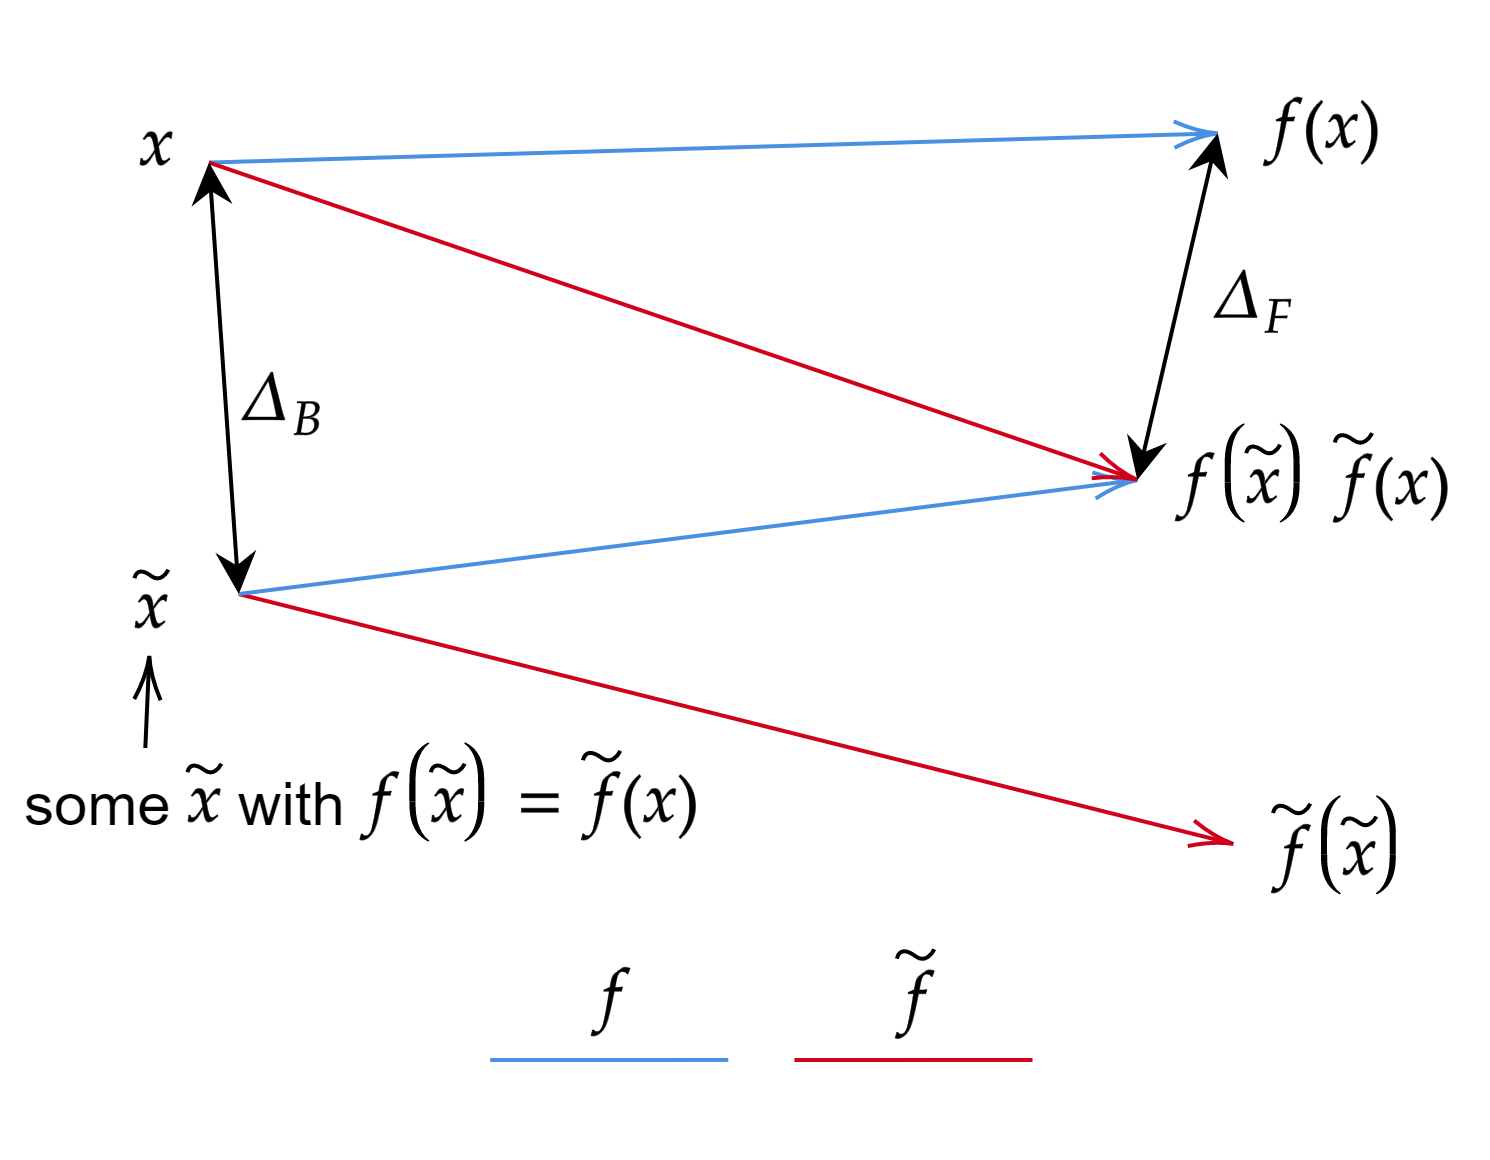
\includegraphics[width=0.45\linewidth]{sections/images/ForwardError.png}
    \caption{Illustration of Forward/Backward Error}
\end{figure}

\end{itemize}
    \item (Forward) Stability: An algorithm $ \tilde{f} $ is stable if \index{Forward Stability}
    \begin{align}
        \dfrac{\Vert \tilde{f}(x)-f(\tilde{x})\Vert }{\Vert f(\tilde{x})\Vert }=O(\varepsilon _\mathrm{machine} ),\,\forall \dfrac{\Vert \tilde{x}-x\Vert }{\Vert x\Vert }=O(\varepsilon _\mathrm{machine} ) 
    \end{align}
    \item Condition Number of problem $ f $:\index{Condition Number}
    \begin{itemize}[topsep=2pt,itemsep=0pt]
        \item Absolute condition number:
        \begin{align}
            \hat{\kappa }(x)=\lim_{\varepsilon \to 0}\mathop{\sup}\limits_{\Vert \delta x\Vert <\varepsilon }\dfrac{\Vert\delta f(x)\Vert}{\Vert\delta x\Vert}=\left\Vert \dfrac{\partial^{} f}{\partial x^{}}\right\Vert   
        \end{align}
        \item Relative condition number:
        \begin{align}
            \kappa (x)=\lim_{\varepsilon \to 0} \mathop{\sup}\limits_{\Vert \delta x\Vert <\varepsilon }\dfrac{\Vert \delta f\Vert \big/\Vert f\Vert }{\Vert \delta x\Vert \big/\Vert x\Vert }
        \end{align}
    \end{itemize}

    (Relative) Condition Number of Matrix $ \mathop{A}\limits_{m\times m}  $: 
    \begin{itemize}[topsep=2pt,itemsep=0pt]
        \item $ f(x)\equiv Ax $:
        \begin{align}
            \kappa =\Vert A\Vert \dfrac{ \Vert x\Vert }{\Vert Ax\Vert }\leq \Vert A\Vert \Vert A^{-1}\Vert  
        \end{align}
        \item $ f(b)\equiv  $ solving $ Ax=b $
        
        \begin{align}
            \kappa = \Vert A^{-1}\Vert \dfrac{\Vert b\Vert }{\Vert x\Vert }\leq \Vert A^{-1}\Vert \Vert A\Vert 
        \end{align}
    \end{itemize}
    
        Thus for matrix $ A $, denote 
        \begin{align}
            \kappa  (A)\equiv \Vert A\Vert\Vert A^{-1}\Vert 
        \end{align}
        
    \begin{itemize}[topsep=2pt,itemsep=0pt]
        \item For $ \ell_2 $ norm $ \Vert\cdot\Vert_2 $: $ \kappa (A)=\dfrac{\sigma  _1}{\sigma  _m} $\footnote{Knowledge about matrix norm see \autoref{SubSubSectionMatrixNotationAndLemma}}
    \end{itemize}
\end{itemize}


    
\subsubsection{Iteration Algorithm}
    Iteration methods are used especially for problems without analytical solution, to obtain a numerical solution.

    Iteration method: for problem $ f $ with solution $ x^* $ design an iteration function $ g $: $ X\to X $ so that 
    \begin{align}
        \lim_{n\to\infty}g^{\{n\}}(x)=\lim_{n\to\infty}\mathop{\underbrace{g(g(g(\ldots g(g}}\limits_{n}(x))\ldots ))) =x^*
    \end{align}
    
    then get solution by setting initial input value $ x^{(0)} $ and calculate $ x^{(t+1)}=g(x^{(t)}) $ repeatedly until convergence as approximate solution.
    
\begin{point}
    Three Steps for Iteration:
\end{point}

\begin{algorithm}{General Steps for Iteration}
    \begin{enumerate}[topsep=2pt,itemsep=2pt]
        \item Starting: set $ x^{(0)} $, more trials to initial value is recommended
        \item Updating: $ x^{(t+1)}=g(x^{(t)}) ,\,\forall t=0,1,2,\ldots$
        \item Stopping: when to stop, can choose various stopping criterion, e.g.
        \begin{itemize}[topsep=2pt,itemsep=0pt]
            \item Absolute convergence criterion
            \begin{align}
                |x^{(t+1)}-x^{(t)}|<\varepsilon  
            \end{align}
            
            \item Relative convergence criterion
            \begin{align}
                \dfrac{|x^{(t+1)}-x^{(t)}|}{|x^{(t)}|}< \phi 
            \end{align}
            
            \item Relative convergence criterion (2), avoid $ x^{(t)}=0 $
            \begin{align}
                \dfrac{|x^{(t+1)}-x^{(t)}|}{|x^{(t)}|+\xi }< \phi 
            \end{align}        
        \end{itemize}
    \end{enumerate}
\end{algorithm}
    



    
\begin{point}
    Convergence Order and Convergence Rate
\end{point}\index{Convergence Order}

    For each iteration value $ x^{(t)} $, define iteration error as $ \varepsilon ^{(t)}\equiv x^{(t)}-x^* $. Then an iteration method $ \lim_{t\to \infty}\varepsilon ^{(t)}=0 $ has convergence order $ \alpha  $ and convergence rate $ c $ as:
    \begin{align}
        \lim_{t\to\infty}\dfrac{|\varepsilon ^{(t+1)}|}{|\varepsilon ^{(t)}|^\alpha }=c 
    \end{align}
    
     A large $ \alpha  $ and small $ c $ declare a quick convergence.(Large $ \alpha  $ is needed more)

    Comment: Actually convergence rate and order are generally dependent on specific problem, so we usually estimate $ \alpha  $, $ c $ using some approximation/scaling to represent a generally case.

\subsubsection{Constrained Optimize Theory}
\begin{point}
    Primal Problem\index{Primal Problem}
\end{point}


    For optimize problem in convex set $ \mathcal{X} $
\begin{align}
        \mathop{\arg\min}\limits_{x\in\mathcal{X}}\quad &f(x)\tag{P}\\
        s.t.\quad   &g_i(x)\leq 0,\quad i=1,2,\ldots,k\\
        & h_j(x)=0,\quad j=1,2,\ldots,l
\end{align}

    which is called the \textbf{primal problem} for optimization.\index{Primal Problem}
    
    The \textbf{generalized Lagrange function} for primal problem defined as \index{Generalized Lagrange Function}
\begin{equation}\label{EqaGeneralizedLagrangeFunction}
 \begin{aligned}
    \mathcal{L}(x,\kappa ,\lambda )\equiv& f(x)+\sum_{i=1}^k\kappa _ig_i(x)+\sum_{j=1}^l\lambda _jh_j(x) \\
    w.r.t. \quad&\kappa _i\geq 0,\quad i=1,2,\ldots,k
\end{aligned}   
\end{equation}

        
    and we could further define a function of $ x $:
\begin{align}
    \theta _P(x)\equiv& \mathop{\max}\limits_{\kappa ,\lambda :\kappa _i\geq 0}\mathcal{L}(x,\kappa ,\lambda ) =\begin{cases}
            f(x)&\text{constraint } g,\,h \text{ satisfied}\\
            +\infty &\text{contraint unsatisfied}
        \end{cases}
\end{align}
       
    which means we can give the solution value of primal problem (P) simply by minimizing $ \theta _P(x) $, minimum denoted $ p^* $
    \begin{align}
        p^* \equiv \mathop{\min}\limits_{x}\theta _P(x)=\mathop{\min}\limits_{x}  \mathop{\max}\limits_{\kappa ,\lambda :\kappa _i\geq 0}\mathcal{L}(x,\kappa ,\lambda )
    \end{align}
    
\begin{point}
    Dual Problem\index{Dual Problem}
\end{point}

    Similar to primal problem, we can define a function of $ \kappa ,\lambda  $:
\begin{align}
    \theta _D(\kappa ,\lambda )\equiv&\mathop{\min}\limits_{x} \mathcal{L}(x,\kappa ,\lambda )
\end{align}

    and similarly get the \textbf{dual problem} of primal, value denoted $ d^* $\index{Lagrange Dual Problem}\index{Dual Problem}
\begin{align}
    d^*\equiv\max_{\kappa ,\lambda :\kappa \geq 0}\theta _D(\kappa ,\lambda )=\max_{\kappa ,\lambda :\kappa \geq 0}\mathop{\min}\limits_{x} \mathcal{L}(x,\kappa ,\lambda )
\end{align} 
    
    it is obvious that 
    \begin{align}
        d^*= \max_{\kappa ,\lambda :\kappa \geq 0}\mathop{\min}\limits_{x} \mathcal{L}(x,\kappa ,\lambda ){\color{red}\leq }\mathop{\min}\limits_{x}  \mathop{\max}\limits_{\kappa ,\lambda :\kappa _i\geq 0}\mathcal{L}(x,\kappa ,\lambda )=p^*
    \end{align}
    
\begin{point}
    Karush-Kuhn-Tucker Condition (KKT Condition)\index{KKT Condition (Karush-Kuhn-Tucker Condition)}
\end{point}

    KKT condition to allow $ d^*=p^* $ at $ (x^*,\kappa ^*,\lambda ^*) $: in the case that
\begin{itemize}[topsep=2pt,itemsep=0pt]
    \item $ f(x) $ and $ g_i(x) $ are convex
    \item $ h_j(x) $ in the form of affine function $ A_jx+b $
    \item $ g_i(x) $ are feasible constraints
\end{itemize}

    then $ \mathrm{KKT}\,\Leftrightarrow\, p^*=d^*=\mathcal{L}(x^*,\kappa ^*,\lambda ^*)  $.

    the KKT conditions are:
\begin{equation}\label{EqaKKTCondition}
    \begin{aligned}
    &\nabla_x\mathcal{L}(x^*,\kappa ^*,\lambda ^*)=0&\\
    &\kappa ^*_ig_i(x^*)=0&i=1,2,\ldots,k\\
    &g_i(x^*)\leq 0&i=1,2,\ldots,k\\
    &\kappa _i\geq 0&i=1,2,\ldots,k\\
    &\lambda _j(x^*)=0&j=1,2,\ldots,l
    \end{aligned}
\end{equation}

    
    
    
     







\subsection{Algebratic Problem in Statistics}\label{SubSectionAlgebraticProblemInStatistics}
   Considering the data structure and algorithm implement, many fundamental problems in statistics are basically algebratic problem, e.g.

\begin{itemize}[topsep=2pt,itemsep=0pt]
    \item Matrix multiplication:
    
    \begin{align}
        y=Ax,\,\text{solve } y 
    \end{align}
    \item Linear equation solution:
    \begin{align}
        b=Ax=\sum_{i=1}^nx_ia_i,\, \text{solve } x
    \end{align}
    \item OLS solution:
    \begin{align}
        \hat{\beta }=(X'X)^{-1}XY 
    \end{align}
\end{itemize}

    Generally speaking matrix $ A $ can be constructed in an arbitrary form, so an algorithm implementation needs \textbf{matrix composition} so that we have a better form to handle.
    




\subsubsection{Matrix Operation}
\begin{itemize}[topsep=2pt,itemsep=0pt]
    \item Inverse Matrix: Inverse matrix of $ A=[a_1,\ldots,a_m] $ satisfies
    \begin{align}
        A^{-1}A=AA^{-1}=I 
    \end{align}

    then $ Ax=b\Leftrightarrow x= A^{-1}b$    

    Or generally speaking, solve inverse matrix $ A^{-1}=[\alpha_1,\ldots,\alpha _m] $ is solving linear equations 
    \begin{align}
        A\alpha _i=e_i
    \end{align}
    
    In the view of column space transfrom, $ A $ and $ A^{-1} $ are mappings between space $ \mathrm{span}\{e_1,\ldots,e_m\}  $ and $ \mathrm{span}\{a_1,\ldots,a_m\}  $, i.e.
    \begin{align}
        \mathrm{span}\{e_1,\ldots,e_m\} \mathop{\rightleftharpoons }\limits_{A^{-1}b}^{Ax}  \mathrm{span}\{a_1,\ldots,a_m\}
    \end{align}
    
    \item Unitary Matrix: Furthur for unitary $ A $, denoted as $ Q $ with $ QQ^*=I $, is an orthonormal transformation.
\begin{itemize}[topsep=2pt,itemsep=0pt]
    \item $ |Q|=1 $ for rotation, $ |Q|=-1 $ for reflection.
    \item $ \lambda_Q=\pm 1 $
    \item Geometric structure preserved, e.g. inner product and norm.
\end{itemize}

    \item Projection: \index{Projection Operator}
    \begin{itemize}
        \item Basic definition of projector $ P_X $: idempotent matrix, project onto hyperplane $ X $ 
        \begin{align}
            P_X^2=P_X 
        \end{align}        
        \item Complementary projector $ I-P_X $: onto the complementary space of $ X $
        \begin{align}
             (I-P)^2=I-P
        \end{align}
        \item Orthogonal Projection: Projector such that $ Pv\perp (I-P)v $. Thm.: $ Pv\perp (I-P)v\Leftrightarrow P^*=P $
        
        Derivation: Projection of vector $ v $ on hyperplane $ X $ satisties (denoted as $ Xp $)
        \begin{align}
            0=\langle Xp,Xp-v\rangle=p^*X^*(Xp-v)\Rightarrow p=(X^*X)^{-1}Xv\Rightarrow Xp={\color{red}X(X^*X)^{-1}X}v={\color{red}P_X}v
        \end{align}
        
        More Properties of orthogonal projector see \autoref{SubSubSectionStatisticalInferenceInMultiLRA}.
        \item Orthogonal projector onto vector $ q $:
        \begin{align}
            P_q=q(q^*q)^{-1}q^*=\dfrac{qq^*}{\Vert q \Vert^2_2 } 
        \end{align}
        
        
    \end{itemize}



\end{itemize}

% \subsubsection{Solution to System of Equations}
%     Solve system of linear equations:
%     \begin{align}
%         x=\arg\{Ax=b\} 
%     \end{align}
    
% \begin{itemize}[topsep=2pt,itemsep=0pt]
%     \item $ LU $ decomposition algorithm:
%     \begin{enumerate}[topsep=2pt,itemsep=2pt]
%         \item 
%     \end{enumerate}
    
        
%     \item $ QR $ decomposition algorithm:
%     \begin{enumerate}[topsep=2pt,itemsep=2pt]
%         \item Use e.g. Householder reflector to compute a $ QR $ decomposition of $ A $:
%         \begin{align}
%             A=QR\Rightarrow QRx=b 
%         \end{align}
        
%         \item Use orthonormality of $ Q $: computation complexity $ \sim 2mn^2-\dfrac{2}{3}n^3 $
%         \begin{align}
%             Rx=Q^*b =\xi
%         \end{align}
%         \item Solve $ Rx-\xi  $ to get $ x $.
        
        
%     \end{enumerate}
    
        
% \end{itemize}

    






\subsubsection{Projection and Least Square Problem}
    Recall: Linear model $ Y=X\beta +\varepsilon  $, basically solving linear equation $ Y=X\beta  $, however generally $ Y\notin \mathrm{span}(X)  $, then we use OLS method to reach an estimation of $ \beta$    :
    \begin{align}
        \hat{\beta }=\mathop{\arg\min}\limits_{\beta }\Vert Y-X\beta  \Vert^2
    \end{align}
    
    where for $ \Vert \cdot \Vert = \ell_2 $-norm, $ X\hat{\beta } $ is the projection of $ X\beta  $ onto hyperplane $ X $:
    \begin{align}
        X\hat{\beta }= X(X^*X)^{-1}X^*Y\equiv HY=P_XY
    \end{align}

    For non-full rank $ A=X^*X $: use pseudoinverse $ A^+=(A^*A)^{-1}A^* $
    
    % Derivation: Projection of vector $ v $ on hyperplane $ X $ satisties (denoted as $ Xp $)
    % \begin{align}
    %      0=<Xp,Xp-v>=p^*X^*(Xp-v)\Rightarrow p=(X^*X)^{-1}Xv\Rightarrow Xp=X(X^*X)^{-1}Xv=P_Xv
    % \end{align}
    
    % Properties:(see \autoref{SubSubSectionStatisticalInferenceInMultiLRA})
    % \begin{itemize}[topsep=2pt,itemsep=2pt]
    %     \item Hermite: $ P_X^*=P_X $;
    %     \item Idempotence: $ P_X^2=P_X $
    %     \item Rank: $ \mathrm{rk}(P_X)=tr(P_X)=\mathrm{rk}(X)$
    %     \item Space of $ P $:
    %     \begin{itemize}[topsep=2pt,itemsep=0pt]
    %         \item $ \mathrm{Im}(I-P)=\mathcal{N}(P) $
    %         \item $ \mathrm{Im}(P)=\mathcal{N}(I-P)  $
    %     \end{itemize}
    % \end{itemize}
    
    % Projection on vector $ q $:
    % \begin{align}
    %     P_q=q(q^*q)^{-1}q^*=\dfrac{qq^*}{\Vert q \Vert } 
    % \end{align}


\begin{point}
    Task of OLS (Linear Model): Solve $ \hat{\beta }=(X^*X)^{-1}X^*Y $, or equivalently solve $ X^*X\hat{\beta }=X^*Y $
\end{point}

    Note: size of matrix denoted $ X=\mathop{X}\limits_{m\times n}  $
    % Algorithm using $ QR $ decomposition:
\begin{itemize}[topsep=2pt,itemsep=0pt]
    \item Cholesky decomposition algorithm: computation complexity $ \sim mn^2+\dfrac{n^3}{3} $
    \begin{enumerate}[topsep=2pt,itemsep=2pt]
        \item Use Cholesky decomposition for $ X^*X $:
        \begin{align}
            A^*A=R^*R\Rightarrow R^*R\hat{\beta }=X^*Y 
        \end{align}
        \item Solve $ \xi =\arg\{ R^*\xi =X^*Y \} $:
        \begin{align}
            R^*R\hat{\beta }=X^*Y=R^*\xi \Rightarrow R\hat{\beta }=\xi  
        \end{align}
        \item Solve $ R\hat{\beta }=\xi  $ to get $ \hat{\beta } $
    \end{enumerate}
    \item $ QR $ decomposition algorithm: computation complexity $ \sim 2mn^2-\dfrac{2}{3}n^3 $
    \begin{enumerate}[topsep=2pt,itemsep=2pt]
        \item Use e.g. Householder Reflection algorithm to compute $ X=QR $
        \item use the orthonormal property of $ Q $:
        \begin{align}
            X^*X\hat{\beta }=X^*Y\Rightarrow R^*Q^*QR\hat{\beta }=R^*R\hat{\beta }=R^*Q^*Y\Rightarrow R\hat{\beta }=Q^*Y 
        \end{align}
        \item Solve $ R\hat{\beta }=Q^*Y $ to get $ \hat{\beta } $
    \end{enumerate}
    \item SVD algorithm: computation complexity $ \sim 2mn^2+11n^3 $
    \begin{enumerate}[topsep=2pt,itemsep=2pt]
        \item Compute SVD of $ X $: $ X=U\Sigma V^* $
        \begin{align}
             X^*X\hat{\beta }=X^*Y\Rightarrow V\Sigma ^2V^*\hat{\beta }=V\Sigma U^*Y\Rightarrow \Sigma V^*\hat{\beta }=U^*Y
        \end{align}
        \item Solve $ \hat{\beta }=V\Sigma ^{-1}U^*Y $ to get $ \hat{\beta } $
    \end{enumerate}
    
\end{itemize}
    
    Algorithm comparison \& trade-off: faster $ \leftrightsquigarrow $ less stable.



\subsubsection{Gaussian $ LU $ Decomposition \& Cholesky Decomposition}
\begin{point}
    Gaussian Elimination Algorithm
\end{point}

    Gaussian Elimination decomposes matrix $ A $ as lower triangular matrix $ \times $ upper triangular matrix
    \begin{align}
        \mathop{A}\limits_{m\times m}=\mathop{L}\limits_{m\times m}\mathop{U}\limits_{m\times m}  =
        \begin{bmatrix}
            *&&&\\
            *&*&&\\
            \vdots&\vdots&\ddots&\\
            *&*&\ldots&*
        \end{bmatrix}
        \begin{bmatrix}
            *&*&\ldots &*\\
            &*&\ldots&*\\
            &&\ddots&\vdots\\
            &&&*
        \end{bmatrix}  
    \end{align}
    
    Conducted by continuously row transformation of $ A $:
    \begin{align}
        L_{m-1}\ldots L_2L_1A=L^{-1}A=U 
    \end{align}
    
    where each $ L_i $ corresponds to a gauss elimination operation such that $ \left[L_i(L_{i-1}\ldots L_2L_1A)\right]_{i+1:m,i}=0 $, with $\left[L_i(L_{i-1}\ldots L_2L_1A)\right]_{1:i,:} $ fixed. $ L_i $ has the form as 
    \begin{align}
        L_i=I-l_ie_i^*,\qquad l_i=[0,\ldots,l_{i+1,i},\ldots,l_{m,i}]^T\quad l_{j,i}=A_{ji}/A_{ii}
    \end{align}
    
    Then we have $ L=L_1^{-1}L_2^{-1}\ldots L_{m-1}^{-1}U $, with $ U=L_{m-1}\ldots L_2L_1A $

    If some pivot element $ (L_{i-1}\ldots L_1A)_{ii}=0 $, use a row transformation $ P_i $ such that $ (P_iL_{i-1}\ldots L_1A)_{ii}\neq 0 $, thus $ LU $ decomposition is expanded as 
    \begin{align}
        L_{m-1}P_{m-1}\ldots L_2P_2L_1P_1A=U
    \end{align}

    Good properties of $ L_i=I-l_ie_i^* $: enable a quick algorithm implement of $ LU $ decomposition:
    \begin{itemize}[topsep=2pt,itemsep=0pt]
        \item Inverse of $ L_i $:
        \begin{align}
            L_i^{-1}=(I-l_ie_i^*)^{-1}=I+l_ie_i^* 
        \end{align}
        \item Multiplication of $ L_i^{-1} $:
        \begin{align}
            L_i ^{-1}L_{i+1}^{-1}=(I+l_ie_i^*)(I+l_{i+1}e_{i+1}^*)=I+l_ie_i^*+l_{i+1}e_{i+1}^*
        \end{align}
        \item Interchangeability of $ P_i $ and $ L_j $ :
        % (note that $ P_i^2=I $):
        \begin{align}
            L_{m-1}P_{m-1}\ldots L_2P_2L_1P_1=(\tilde{L}_{m-1}\ldots\tilde{L}_2\tilde{L}_1)(P_{m-1}\ldots P_2P_1),\qquad \tilde{L}_i=P_{m-1}\ldots P_{i+1}L_iP^{-1}_{i+1}\ldots P^{-1}_{m-1}
        \end{align}        
        where note that $ P_{k} $ only exchange row/column $ k $ and $ \kappa>k $, thus $ \tilde{L}_i $ is still left triangular.
    \end{itemize}
    
    \noindent Thus get expression of $ LU $ decomposition $ PA=LU $:
    \begin{align}
         PA=LU\quad\begin{cases}
            P=P_{m-1}\ldots P_2P_1\\
            L= (\tilde{L}_{m-1}\ldots\tilde{L}_2\tilde{L}_1)^{-1}\\
            \tilde{L}_i=P_{m-1}\ldots P_{i+1}L_iP_{i+1}\ldots P_{m-1}\\
            U=L_{m-1}P_m\ldots L_2P_2L_1P_1A
         \end{cases} 
    \end{align}
    
    

    Complexity of Gaussian Elimination:
    \begin{align}
        \mathrm{flops}_\mathrm{GE}=&\sum_{i=1}^{m-1}\sum_{k=i+1}^m 2(m-i+1)\sim \dfrac{2}{3}m^3
    \end{align}
 
\begin{point}
    Cholesky Decomposition
\end{point}

    Hermitian positive-definite matrix $ A $ can $ LU $ decompose as
    \begin{align}
        A=LU=R^*R
    \end{align}
    
    Algorithm: write $ A $ in partitioned matrix then conduct symmetric row/column transformation
    
\begin{align}
    A=&\begin{bmatrix}
      1&w_1^*\\
      w_1&K
    \end{bmatrix}
    \\
    =&\begin{bmatrix}
    1&0\\w_1&I
    \end{bmatrix}
    \begin{bmatrix}
    1&0\\0&K-w_1w_1^*
    \end{bmatrix}
    \begin{bmatrix}
    1&w_1^*\\0&I
    \end{bmatrix}\\
    =&R_1^*K_1R_1
  \end{align} 
    

    Note that $ K_1 $ is still hermite positive-definite, we can repeat the above process
    
        \begin{align}
            K_1=&\
            \begin{bmatrix}
            1&0\\0&K-w_1w_1^*
            \end{bmatrix}\\
            =&\begin{bmatrix}
            1&0&0\\
            0&1&0\\
            0&w_2&I
            \end{bmatrix}
            \begin{bmatrix}
            1&0&0\\
            0&1&0\\
            0&0&K-w_1w_1^*-w_2w_2^*
            \end{bmatrix}
            \begin{bmatrix}
            1&0&0\\
            0&1&w_2^*\\
            0&0&I
            \end{bmatrix}\\
            =&R_2^*K_2R_2
          \end{align} 
    

    repeat untill $ K_m=I $: $ A=(R_mR_{m-1}\ldots R_1)^*I(R_mR_{m-1}\ldots R_1)=R^*R $
    
    Complexity of Cholesky Decomposition:
    \begin{align}
        \mathrm{flops}_\mathrm{CD}=&\sum_{i=1}^{m}\sum_{k=i}^m 2(m-k+1)+1 \sim \dfrac{1}{3}m^3
    \end{align}
 
    
    









    



\subsubsection{$ QR $ Decomposition: Gram-Schmidt/Householder/Givens Method}
    
    $ QR $ Decomposition: Orthogonal Triangularization of matrix $ A $
\begin{align}
    \mathop{A}\limits_{m\times n} =\mathop{Q}\limits_{m\times n} \mathop{R}\limits_{n\times n}     
\end{align}


\begin{align}
    A=\begin{bmatrix}
        a_1&\ldots &a_n
    \end{bmatrix} 
    =QR=
    \begin{bmatrix}
        q_1&\ldots&q_n
    \end{bmatrix}
    \begin{bmatrix}
        r_{11}&r_{12}&\ldots&r_{1n}\\
        &r_{22}&\ldots&r_{2n}\\
        &&\ddots&\vdots\\
        &&&r_{nn}
    \end{bmatrix}
\end{align}

    Every $ \mathop{A}\limits_{m\times n} \in \mathbb{C}^{m\times n} $ ($ m\geq n $) has $ QR $ decomposition, specially:
    \begin{itemize}[topsep=2pt,itemsep=0pt]
        \item Full decomposition exists
        \item Reduced decomposition with $ r_{ii}>0 $ is unique.
        % \item If $ A\in\mathbb{R}^{m\times n} $, then $ U\in\mathbb{R}^{m\times n} $, 
    \end{itemize}
    
        
% \Leftrightarrow\begin{cases}
    %     Q=AR^{-1}&\mathrm{span}\text{ of }A\\
    %     R=Q^{-1}A&\text{Orthogonal Triangularization}
    % \end{cases} 
    Here introduce 3 kinds of algorithm:
    \begin{itemize}[topsep=2pt,itemsep=0pt]
        \item \hyperlink{GS-Decomposition}{Gram-Schmidt Orthogonalization}: $ \sim O(2mn^2) $, sequentially orthogonalizes the columns of $ A $, traditional way
        \item[$ \color{red}\star $] \hyperlink{Householder-Reflection}{Householder Reflection}: $ \sim O(2mn^2-\dfrac{2}{3}n^3) $, most commonly used, stable for ill \& dense matrix
        \item \hyperlink{Givens-Rotation}{Givens Rotation}: $ \sim O(3mn^2-n^3) $, used for sparse matrix, e.g. Hessenberg matrix
    \end{itemize}
    
        




\begin{point}
    \hypertarget{GS-Decomposition}{(Classical) Gram-Schmidt Orthogonalization}\index{CGS (Classical Gram-Schmidt Orthogonalization)}
\end{point}

    Key idea: project $ a_i $ onto $ \mathrm{span}\{q_1,\ldots,q_{i-1}\}^\perp  $ as $ q_i $, with $ q_1 $ initialized as $ \hat{a}_1 $, projection coefficient $ r_{ij} $ forms $ R $.

    For each projection, the projector matrix is 
    \begin{equation}\label{EqaCGSProjector}
        P_i=I-\sum_{k=1}^{i-1}q_kq_k^*      
    \end{equation}
    
    expression of $ q_i $ and $ r_{ij} $: 

\begin{align}
    r_{ij}=\begin{cases}
        q_i^*a_j&i\neq j\\
        \Vert a_i-\sum_{k=1}^{i-1}r_{ki}q_k \Vert& i=j 
    \end{cases}\qquad 
    q_i=\dfrac{a_i-\sum_{k=1}^{i-1}r_{ki}q_k}{r_{ii}}=\dfrac{a_i-\sum_{k=1}^{i-1}q_kq_k^*a_i}{\Vert a_i-\sum_{k=1}^{i-1}q_kq_k^*a_i \Vert }
\end{align}

    Note: Algorithm implementation of $ q_i $ is $ (q_{<i})\to r_{k<i,i}\to q_{i}\& r_{ii} \to (q_{>i}) $


\begin{point}
    Modified Gram-Schmidt Orthogonalization Algorithm\index{MGS (Modified Gram-Schmidt Orthogonalization)}
\end{point}

    In \autoref{EqaCGSProjector}, projection of G-S orthogonalization for each $ a_i $ is conducted `simultaneously', while modified G-S decomposition is conducted step by step.

\begin{align}
    P_i=I-\sum_{k=1}^{i-1}q_kq_k^*=\prod_{k=1}^{i-1}(I-q_kq_k^*) 
\end{align}
    
    Decomsition result are the same, but modified algorithm is more stable for numerical computation, avoid problem of recursive $ q_i $.


\begin{rcode}
    Algorithm of CGS/MGS
\begin{lstlisting}[language=R]
GS <- function(A,MGS=FALSE){
    stopifnot(is.matrix(A))
    m <- dim(A)[[1]]
    n <- dim(A)[[2]]
    v=matrix(0,nrow = m,ncol=m)
    r=matrix(0,nrow = m,ncol=n)
    q=matrix(0,nrow = m,ncol=m)
    for(j in 1:n){
        v[,j] <- A[,j]
        if(j>1){
        for(i in 1:(j-1)){
          r[i,j]=sum(q[,i]*ifelse(MGS,v[,j],A[,j]))#对MGS取v,CGS取a
          v[,j] <- v[,j]-r[i,j]*q[,i]
        }}
        r[j,j] <- sqrt(sum(v[,j]^2))
        q[,j] <- v[,j]/r[j,j]
    }
  return(list(q,r))
}
\end{lstlisting}
\end{rcode}






\begin{point}
    \hypertarget{Householder-Reflection}{Householder Reflection}
\end{point}

    Key idea: Reflect $ A_{i:m,i} $ onto $ e_{1}\in\mathbb{C}^{m-i+1} $ as a vector of the same length $ \Vert  A_{i:m,i} \Vert e_{1}\in\mathbb{C}^{m-i+1} $ (later we denote the $ l^\mathrm{th}  $ unit vector $ e_{l}\in\mathbb{C}^{m-i+1}\equiv e_{m-i+1,l} $), reflector $ F_i $ in $ \mathbb{C}^{(m-i+1)\times (m-i+1)} $ and auxiliary vector $ v_i $:\footnote{Here $ \mathrm{sgn}() $ for reflecting toward $ -e_1 $/$ e_1 $.}
    \begin{align}
        \mathbb{C}^{(m-i+1)\times( m-i+1)} \ni F_i=I_{m-i+1}-2\dfrac{vv^*\,}{\Vert v \Vert_2^2 }\qquad v= \mathrm{sgn}(A_{i,i}) \Vert  A_{i:m,i} \Vert e_{m-i+1,1}+ A_{i:m,i} 
    \end{align}

    where $ \mathrm{sgn}(\cdot) $ corresponds to reflection onto $ \hat{e} $ or $ -\hat{e} $.   
    Reflector on $ A\in\mathbb{C}^{m\times n} $:
    \begin{align}
        Q_i=\begin{bmatrix}
            I_{i-1}&0\\
            0&F_i
        \end{bmatrix} 
    \end{align}
    
    and $ QR $ calculated by (note that $ F^2=I_{m-i+1} $)
    \begin{align}
        R=Q_n\ldots Q_2Q_1A\qquad Q=Q_1Q_2\ldots Q_n
    \end{align}
    
    

    Householder Reflection is more stable than Gram-Schimidt Orthogonalization


    
    
    Error of Householder Reflection $ A=\tilde{Q}\tilde{R}+E $, residual is controlled by $ \Vert E \Vert \leq \Vert A \Vert O(\varepsilon _\mathrm{machine}) $

    Mainly caused by stability and accuracy of orthogonal matrix $ \tilde{Q} $.
    % GS: $ a $


\begin{rcode}
\lstinline|R.| uses Householder Reflection to conduct $ QR $ decomposition.
\begin{lstlisting}[language=R]
A.qr <- qr(A)
Q <- qr.Q(A.qr)
R <- qr.R(A.qr)
\end{lstlisting}
\end{rcode}

\begin{point}
    \hypertarget{Givens-Rotation}{Givens Rotation}
\end{point}
    
    Key idea: use rotation
    \begin{align}
        Rx=\begin{bmatrix}
            \cos\theta &-\sin\theta \\
            \sin\theta &\cos\theta 
        \end{bmatrix} \begin{bmatrix}
            x_i\\x_j
        \end{bmatrix}=\begin{bmatrix}
            \sqrt{x_i^2+x_j^2}\\0
        \end{bmatrix}
        \Leftrightarrow \begin{cases}
            \cos\theta =\dfrac{x_i}{\sqrt{x_i^2+x_j^2}}\\
            \sin\theta =\dfrac{x_j}{\sqrt{x_i^2+x_j^2}}
        \end{cases}
    \end{align}
    
    act on $ A_{i-1:i,j:n} $ so that $ A_{i,j}=0 $, each time use two rows to create 1 zero. Slow, used for special sparse matrix.
    
\subsubsection{Eigenvalue Decomposition}
    For square matrix $ A \in\mathbb{C}^{m\times m}$, its eigenvector is the vector $ x_i $ whose direction (subspace) is invariant under transform operator $ A $.
    \begin{align}
        Ax_i =\lambda _ix_i
    \end{align}
    
    Properties:
\begin{itemize}[topsep=2pt,itemsep=0pt]
    \item Determinant and trace of $ A $:
    \begin{align}
        \det(A)=\prod_{i=1}^m\lambda _i\qquad tr(A)=\sum_{i=1}^m\lambda _i 
    \end{align}
    \item $ x_i $ for special kinds of $ A $: if $ \mathrm{span}\{q_i\}=\mathbb{C}^m  $, then (generally $ X $ is \textbf{not} orthogonal)
    \begin{align}
        AX=X\Lambda \Rightarrow  A=X\Lambda X^{-1} 
    \end{align}
    
    
    Further for $ AA^*=A^*A $ (Normal Matrix\index{Normal Matrix} 规范矩阵. Include: hermitian $ A=A^* $\index{Hermitian Matrix}, skew hermitian $A=-A^* $, unitary $ A^{-1}=A^* $, circulant matrix\index{Circulant Matrix}\footnote{Circulant Matrix, or similarly Latin Square.
    \begin{align}
        C=\begin{bmatrix}
            c_0&c_1&c_2&c_3\\
            c_3&c_0&c_1&c_2\\
            c_2&c_3&c_0&c_1\\
            c_1&c_2&c_3&c_0
        \end{bmatrix} 
    \end{align}
    
    }, and such $ A+kI $), orthonormality of $ x_i\to q_i $:
    \begin{align}
        \langle q_i,q_j  \rangle =\delta_{ij}
    \end{align}
    Eigenvalue Decomposition/Spectrum Decomposition, $ X\to Q $:
    \begin{align}
        AQ=Q\Lambda \Rightarrow A=Q\Lambda Q^{-1}=Q\Lambda Q^*
    \end{align}
    \item Eigenvalue decomposition and positive definite matrix (Gershgorin circle thm.), $ \lambda _i $ falls in neighbourhood of $ a_{ii} $:
    \begin{align}
        D(\lambda_i,a_{ii})<\sum_{j=1,j\neq i}^m|a_{ij}| 
    \end{align}
    \item Rayleigh quotient:
    \begin{align}
        \max R(A,q)\equiv \max \dfrac{q^*Aq}{q^*q}=\lambda _1 
    \end{align}
    
    
        
\end{itemize}

    






Eigenvactor Algorithm: Power method to find leading eigen pair.

for independent eigenvectors $ x_i $ and an arbitrary vector $ \xi =\sum_{i=1}^mc_ix_i $:
\begin{align}
    A^k\xi =A^k\sum_{i=1}^mc_ix_i=\sum_{i=1}^mc_i\lambda_i^kx_i=c_1\lambda _1^k\left[x_1+\sum_{i=2}^n\dfrac{c_i}{c_1}\left(\dfrac{\lambda _i}{\lambda _1}\right)^kx_i\right]\to c_1\lambda _1^kx_1
\end{align}




\begin{algorithm}{Basic Eigen Decomposition}
    \begin{enumerate}[topsep=2pt,itemsep=0pt]
    \item pick a random $ q_0 $
    \item compute normalized $ \dfrac{Aq_i}{\Vert Aq_i \Vert }=q_{i+1} $
    \item repeat until $ \Vert q_{i-1}-q_{i-2} \Vert<\varepsilon_\mathrm{preset}    $
    \item $ q_i $ as the eigenvector, $ q_i^TAq_i\approx q_i^T\lambda_1 q_i=\lambda _1 $
\end{enumerate}
\end{algorithm}
    


    This algorithm requires $ |\lambda _1|>|\lambda _2|\geq\ldots  $ for quick convergence.
    













\subsubsection{SVD Decomposition}
\begin{point}
    SVD (Singular Value Decomposition)\index{SVD (Singular Value Decomposition)} Form:
\end{point}

    
\begin{itemize}[topsep=2pt,itemsep=0pt]
    \item Reduced Form:
\begin{align}
    \mathop{A}\limits_{m\times n} =\mathop{U}\limits_{m\times n}\mathop{\Sigma }\limits_{n\times n}\mathop{V^*}\limits_{n\times n}     
\end{align}

\begin{align}
    A=\begin{bmatrix}
        a_1&\ldots &a_n
    \end{bmatrix} 
    =U\Sigma V^*=
    \begin{bmatrix}
        u_1&\ldots&u_n
    \end{bmatrix}
    \begin{bmatrix}
        \sigma_1&&&\\
        &\sigma_2&&\\
        &&\ddots&\\
        &&&\sigma_n
    \end{bmatrix}
    \begin{bmatrix}
        v_1^*\\
        v_2^*\\
        \vdots\\
        v_n^*
    \end{bmatrix}
\end{align}
    \item Full Form:

    \begin{align}
        \mathop{A}\limits_{m\times n} =\mathop{U}\limits_{m\times m}\mathop{\Sigma }\limits_{m\times n}\mathop{V^*}\limits_{n\times n}     
    \end{align}
    
    \begin{align}
        A=\begin{bmatrix}
            a_1&\ldots &a_n
        \end{bmatrix} 
        =U\Sigma V^*=
        \begin{bmatrix}
            u_1&u_2&\ldots&u_m
        \end{bmatrix}
        \begin{bmatrix}
            \sigma_1&&&\\
            &\sigma_2&&\\
            &&\ddots&\\
            &&&\sigma_n\\
            0&0&0&0\\
            \vdots&\vdots&\vdots&\vdots
        \end{bmatrix}
        \begin{bmatrix}
            v_1^*\\
            v_2^*\\
            \vdots\\
            v_n^*
        \end{bmatrix}
    \end{align}
\end{itemize}


    Existence and uniqueness of SVD:
\begin{itemize}[topsep=2pt,itemsep=0pt]
    \item Every $ A\in\mathbb{C}^{m\times n} $ has SVD with $ \{\sigma_i\} $ unique
    \begin{align}
        A=U\Sigma V^* =\sum_{i=1}^n\sigma _iu_iv_i^*
    \end{align}
    
    \item if $ A $ is squared, then $ U,V $ determined
    \item if $ A\in\mathbb{R}^{m\times n} $, then $ U,V \in \mathbb{R}$ 
\end{itemize}

\begin{point}
    SVD Expression
\end{point}

    $ U $, $ V $ are eigenvectors of $ AA^* $, $ A^*A $ respectively
\begin{align}
    A^*A=V\Sigma ^2V^*\qquad AA^*=U\Sigma ^2U^*\qquad u_j=\dfrac{Av_j}{\sigma _j}\quad \sigma _j=\sqrt{\lambda _{A^*A}}=\sqrt{\lambda _{AA^*}}
\end{align}

\begin{point}
    Properties of SVD:
\end{point}

   
\begin{itemize}[topsep=2pt,itemsep=0pt]
    \item rank of $ A $: $ r=\mathrm{rk}(\mathop{A}\limits_{m\times n} )=\# \text{ non-zero } \sigma _i  $
    \item Space of $ A  $:
    \begin{itemize}
        \item $ \mathcal{R}(A)=\mathrm{span}\{u_1,\ldots ,u_r\}  $
        \item $ \mathcal{C}(A)=\mathrm{span}\{v_1,\ldots,v_r\}  $
        \item $ \mathcal{N}(A)=\mathrm{span}\{v_{r+1},\ldots,v_n\}  $
    \end{itemize}
    \item Norm:
    \begin{itemize}[topsep=2pt,itemsep=0pt]
        \item Euclidean Norm: $ \Vert A \Vert _2=\sigma _1 $
        \item Frobenius Norm: $ \Vert A \Vert _F=\sqrt{\sum_{i=1}^r\sigma _i^2 } $
        \item Nuclear Norm: $ \Vert A \Vert _*=\sum_{i=1}^r\sigma _i $
    \end{itemize}
    \item Square matrix:
    \begin{itemize}
        \item if $ A=A^* $, then $ \sigma _j=|\lambda _A|_j $
        \item $ \det(A)=\prod_{i=1}^m\sigma _i $
    \end{itemize}
    \item Low-rank Approximation of $ A $ using SVD:
    \begin{align}
        A_k= \sum_{i=1}^k\sigma _iu_iv_i^*=A-\sum_{j=k+1}^r\sigma _ju_jv_j^*
    \end{align}
    
    is the `nearest' rank $ k $ matrix from $ A $ 
    \begin{align}
        \mathop{\min}\limits_{\mathrm{rk}(\Xi)=k }\Vert A-\Xi \Vert _2=\Vert A-A_k \Vert _2=\sigma _{k+1}  
    \end{align}
    
\end{itemize}

\begin{point}
    When $ A $ is positive definite, SVD and ED get the same result.
\end{point}

\begin{align}
    A=Q\Lambda Q^*\Rightarrow  A=Q\mathrm{sgn}(\Lambda )|\Lambda |Q^*=U\Sigma Q^*=U\Sigma V^* 
\end{align}



\subsubsection{Schur Decomposition}
    Unitary Triangularization of matrix $ A $ (always exists in $ \mathbb{C}^{m\times m} $):
    \begin{align}
        A=QTQ^*,\, Q\text{ unitary, }T\text{ upper-triangular} 
    \end{align}
    
    for $ A\in\mathbb{R}^{m\times m} $: $ T $ is quasi-triangular, diag of $ T $ is $ \mathrm{Re} (\lambda _i) $
















\subsection{Numeric Optimization Algorithm I}

Algorithm Optimization in Statistics: e.g.
\begin{itemize}[topsep=2pt,itemsep=0pt]
    \item MLE Maximazation
    \item Linear/Logistics Regression: Minimizing error
    \item Clustering: minimizing within-cluster distance \& maximizing between-cluster distance
    \item Box-Cox $ \lambda  $ determining
    \item Machine Learning Model training, minimizing loss function
\end{itemize}

\begin{point}
Duality of Optimization and Rooting:
\end{point}

\begin{itemize}[topsep=2pt,itemsep=0pt]
    \item Optimization: e.g. minimizing function $ g(x) $:
    \begin{align}
        \arg\min g(x) \leftrightharpoons \arg\{\nabla g(x)=0\}
    \end{align}
    \item Rooting: extract root $ f(x)=0 $:
    \begin{align}
        \arg \{f(x)=0\}\leftrightharpoons \arg\min f(x)^Tf(x) 
    \end{align}   
\end{itemize}

    More specific example: expand function to $ 2^\mathrm{nd}  $ as $ g(x)\approx\dfrac{1}{2}x^TAx-bx+c $ (differnetiation of quadric $ x^TAx $ see \autoref{SubSubSectionMatrixNotationAndLemma})
    \begin{align}
        \arg\min\dfrac{1}{2}x^TAx-bx+c\leftrightharpoons \arg\{\dfrac{A+A^T}{2}x=b\}
    \end{align}


    \fbox{
        \begin{minipage}{0.9\linewidth}
            $ \Delta $ i.e. for optmizing task $ \arg\min g(x) $, we can either minimizing $ g(x) $, or rooting $ f(x)\equiv \nabla g(x) $
        \end{minipage}
    }\\
    
    
\begin{point}
    Algorithm Design Aim:
\end{point}

\begin{itemize}[topsep=2pt,itemsep=0pt]
    \item Robustness: can be applied on various problems
    \item Accuracy: reach solution with great precision, at the same time insensitive to machine error
    \item Efficiency: computer time/storage not required
\end{itemize}

\begin{point}
    Iteration in Optimization Problem
\end{point}

    Usually iteration is used in optmizing problem, by approximate solution $ x^* $ step by step. 
\begin{itemize}[topsep=2pt,itemsep=0pt]
    \item Bracketing method means the solution $ x^* $ is always within some iteration interval $ I^{(t)}=[x_\mathrm{left},x^*,x_\mathrm{right}  ] $, use convergence condition $ m(I^{(t)})<\varepsilon  $ to obtain solution.
    
    % Includes: Golden Search/Fibonacci Serach/Bisection Search/Regula Falsi
    \item Open method: Not necessarily $ x^*\in I^{(t)} $, but convergence using $ d(x^{(t)},x^{(t-1)})<\varepsilon  $. Usually faster than bracketing, but less stable, and sensitive to initial value.
    
    % Includes: Newton Raphson/Secant
    \item Hybird Method: Mixture of bracketing and open according to iteration step feature
    
    % Includes: Brent's method
\end{itemize}







\begin{point}
    Content
\end{point}
\begin{itemize}[topsep=2pt,itemsep=0pt]
    \item \hyperlink{GoldenSection}{Golden Section \& Fibonacci Section Search}: Bracketing method direct search for minimizer;
    \item \hyperlink{Bisection}{Bisection Search}: Bracketing method direct search for root
    \item \hyperlink{Interpolation}{Interpolation Method}: Include either bracketing/open method, approximate function to obtain root/minimizer
    \begin{itemize}[topsep=2pt,itemsep=0pt]
        \item \hyperlink{RegulaFalsi}{Regula Falsi}: Bracketing linear interpolation for rooting
        \item \hyperlink{Secant}{Secant Interpolation}: Open linear interpolation for rooting
        \item \hyperlink{ParabolicInterpolation}{Parabolic Interpolation}: Open parabolic interpolation for minimizing
        \item \hyperlink{InverseQuadric}{Inverse Parabolic Interpolation (IQI)}: Open interpoation for rooting
    \end{itemize}
    
    \item \hyperlink{HybridMethod}{Hybrid Method}: Combination of bracketing method and open interpolation method for rooting. Include Dekker's and Brent's, most used method
    \begin{itemize}[topsep=2pt,itemsep=0pt]
        \item \hyperlink{Dekker}{Dekker's Method}: Hybrid of bisection and secant interpolation method for rooting
        \item[$\color{red}\star$] \hyperlink{Brent}{Brent's Method}: Hybrid of bisection, secant interpolation and IQI for rooting
    \end{itemize}
       
    \item \hyperlink{FixedPoint}{Fixed Point Iteration Method}: Open method for rooting, including univariate and multivariate linear case.
    \begin{itemize}[topsep=2pt,itemsep=0pt]
        \item Univariate Fixed Point Iteration
        \item \hyperlink{JacobiMethod}{Jacobi Method}
        \item \hyperlink{GaussSeidelMethod}{Gauss Seidel Method}
        \item \hyperlink{SORMethod}{Successive Over-Relaxation Method}
    \end{itemize}
    
        
    \item[$\color{red}\star$] \hyperlink{Simplex}{Nelder-Mead Method/Simplex Method}: Open method for minimizer based on simplex iteration
\end{itemize}

    
\begin{point}
    Default Methods in \lstinline|R.| 
\end{point}
\begin{itemize}[topsep=2pt,itemsep=0pt]
    \item \lstinline|optim(VEC_OF_INI_VAR,FUN)|: Nelder-Mead Simplex search method, use \lstinline|method=c('Nelder-Mead',|\\\lstinline|'BFGS','L-BFGS-B','CG','SANN','Brent')| to choose different methods
    \item \lstinline|uniroot(FUN,INTERVAL)|: Brent's Method;
    \item \lstinline|optimize(FUN,INTERVAL)|: Golden Section+Parabolic Interpolation.
\end{itemize}

    
    % \lstinline|optim()|函数默认方法为Nelder-Mead单纯形搜索法。\lstinline|uniroot()|默认用Brent's方法 \lstinline|optimize()|函数默认方法为Golden Section+二次插值法





\subsubsection{Golden Section/Fibonacci Section Search}
\index{Golden Section Search}\index{Fibonacci Section Search}
    \hypertarget{GoldenSection}{Problem}: minimizing univariate function $ g(x) $, within a pre-estimated interval $ [x_1^{(0)},x_4^{(0)}] $. For $ f $ that is undiffernetiable/complicated to compute, this method is often used. 

    Basic idea: within a unimodal interval $ I^{(0)}=[x_1^{(0)},x_4^{(0)}] $ of $ f(x) $, pick two symmetric points $ x_2^{(0)},x_3^{(0)} $ in $ I_0 $ so that 
\begin{equation}\label{EqaRExpressionInGolden}
    x_2^{(0)}-x_1^{(1)}=x_4^{(0)}-x_3^{(0)}=(1- r^{(0)})(x_4^{(0)}-x_1^{(0)}) \quad  r^{(t)}>1/2
\end{equation}
    
    then extreme point should falls in one of $ [x^{(t)}_1,x^{(t)}_3] $ or $ [x^{(t)}_2,x^{(t)}_4] $, iteration the interval by comparing $ g(x_2) $ and $ g(x_3) $: use one of them as the next interval. And for less computation, we hope that one of $ g(x_2^{(t)}) $ of $ g(x_3^{(t)}) $ can be used in step $ t+1 $ as $ g(x_3^{(t+1)}) $ or $ g(x_2^{(t+1)}) $, i.e.
    \begin{align}
        \text{if }g(x_2^{(t)})>g(x_3^{(t)}):&\, [x_1^{(t+1)},x_2^{(t+1)},x_4^{(t+1)}]:= [x_2^{(t)},x_3^{(t)},x_4^{(t)}]\\
        \text{if }g(x_2^{(t)})\leq g(x_3^{(t)}):&\, [x_1^{(t+1)},x_3^{(t+1)},x_3^{(t+1)}]:= [x_1^{(t)},x_2^{(t)},x_3^{(t)}]
        \end{align}


        also use \autoref{EqaRExpressionInGolden}, we have (here use $g(x_2^{(t)})> g(x_3^{(t)}) $ case for derivation)
        \begin{align}
            r^{(t+1)}=\frac{x_4^{(t)}-x_2^{(t)}}{x_4^{(t)}-x_1^{(t)}}=\dfrac{x_4^{(t+1)}-x_2^{(t+1)}}{x_4^{(t+1)}-x_1^{(t+1)}}=\dfrac{x_4^{(t)}-x_3^{(t)}}{x_4^{(t)}-x_2^{(t)}}=\dfrac{1-r^{(t)}}{r^{(t)}}
        \end{align}
        

\begin{algorithm}{Golden Section/Fibonacci Section Search}

\begin{enumerate}[topsep=2pt,itemsep=2pt]
    \item Initialize $ I^{(0)}=[x_1^{(0)},x_4^{(0)}] $ with $ x^*\in I^{0} $
    \item For each step $ x^{(t)} $:
    \begin{enumerate}[topsep=2pt,itemsep=2pt]
        \item Calculate $ r^{(t)} $, and then $ g(x_2^{(t)}) $, $ g(x_{3}^{(t)}) $
        \item compare $ g(x_2^{(t)}) $ and $ g(x_3^{(t)}) $, and update interval    
        \begin{align}
            \text{if }g(x_2^{(t)})>g(x_3^{(t)}):&\, [x_1^{(t+1)},x_2^{(t+1)},x_4^{(t+1)}]\equiv [x_2^{(t)},x_3^{(t)},x_4^{(t)}]\\
            \text{if }g(x_2^{(t)})\leq g(x_3^{(t)}):&\, [x_1^{(t+1)},x_3^{(t+1)},x_4^{(t+1)}]\equiv [x_1^{(t)},x_2^{(t)},x_3^{(t)}]
        \end{align}
    \end{enumerate}
    \item Repeat until convergence $ m(I^{(t)})<\varepsilon  $
\end{enumerate}
    
    % For less computation, we hope that one of $ g(x_2^{(t)}) $ of $ g(x_3^{(t)}) $ can be used in step $ t+1 $ as $ g(x_3^{(t+1)}) $ or $ g(x_2^{(t+1)}) $, i.e.

    Choice of $ r^{(t)} $: for algorithm robustness and avoid ill sequence, we will usually use some special $ r^{(t)} $:
\begin{itemize}[topsep=2pt,itemsep=0pt]
    \item Golden Section Search: use $ r^{(t)}=r=\mathrm{const}$, such $ r $ should satisfies
    \begin{align}
        r=\dfrac{1-r}{r}\Rightarrow r=\dfrac{\sqrt{5}-1}{2}=\dfrac{1}{\phi }\approx 0.618
    \end{align}

    Convergence at  
    \begin{align}
         m(I^{(t)})=r^{t}m(I^{(0)})<\varepsilon
    \end{align}
    
    
    
    \item Fibonacci Section Search: choose for $ t=0 $ as $ r^{(0)}=\dfrac{F_{n-1}}{F_{n}} $, where $ \{F_n\} $ is Fibonacci sequence, then
\begin{align}
    r^{(0)}=&\dfrac{F_{n-1}}{F_n}\\
    r^{(1)}=&\dfrac{1-r^{(0)}}{r^{(0)}}=\dfrac{F_{n-2}}{F_{n-1}}\\
    r^{(2)}=&\dfrac{1-r^{(1)}}{r^{(1)}}=\dfrac{F_{n-3}}{F_{n-2}}\\
    \vdots&\\
    r^{(t)}=&\dfrac{F_{n-t-1}}{F_{n-t}}\\
    \vdots&\\
    r^{(n-3)}=&\dfrac{F_2}{F_3}=\dfrac{1}{2}\,\text{(the last step of iteration)}
\end{align}
    
    To determine the preset $ n $, first use convergence condition 
    \begin{align}
         m(I^{(n-2)})=\prod_{i=0}^{n-3}r^{(i)}m(I^{(0)})=\dfrac{F_2}{F_n}m(I^{(0)})<\varepsilon \Rightarrow \begin{cases}
             F_n>\dfrac{m(I^{(0)})}{\varepsilon }\\
             F_{n-1}<\dfrac{m(I^{(0)})}{\varepsilon }
         \end{cases}
    \end{align}
    
    then conduct iteration, using $ r^{(t)}=\dfrac{F_{n-t-1}}{F_{n-t}} $.
    
\end{itemize}

    
\end{algorithm}
    


    Basically the two methods have similar background, noticing that the eigen equation of Fibonacci sequence is $ x^2=x+1 $, and $ \lim_{n\to \infty}\dfrac{F_{n-1}}{F_n}=\dfrac{\sqrt{5}-1}{2}=\dfrac{1}{\phi } $\footnote{General Formula of Fibonacci sequence:
    \begin{align}
        F_n=\dfrac{1}{\sqrt{5}}\left( (\phi )^n-(-\dfrac{1}{\phi })^n \right) 
    \end{align}
    }

    Can be proven: Golden section need one more iteration call than Fibonacci section:
    \begin{align}
        n_\mathrm{GS}=n_\mathrm{Fib}+1 
    \end{align}

    Convergence order $ \alpha =1 $, rate $ c=\dfrac{1}{\phi } $


 
\subsubsection{Bisection Search Method}
    % Gradient methods are suitable for derivable function $ f $, minimizing $ f $ is equivalent to root finding of $ \nabla f $
\index{Bisection Search}
    \hypertarget{Bisection}{Problem}: rooting univariate function $ f(x) $, with a pre-­estimated interval $ I^{(0)}=[x_1^{(0)},x_2^{(0)}] $, with $ f(x_1^{(0)})f(x_2^{(0)})<0 $

    Idea: Intermediate value thm.: for continuous $ f:[a,b]\to \mathbb{R}  $, $ f(a)f(b)<0\Rightarrow \exists x^*, s.t. f(x^*)=0 $. 

\begin{algorithm}{Bisection Search}
    
\begin{enumerate}[topsep=2pt,itemsep=2pt]
    \item Initialize $ I^{(0)}=[x_1^{(0)},x_2^{(0)}] $ satisfying $ f(x_1^{(0)})f(x_2^{(0)})<0 $
    \item In each iteration $ x^{(t)} $:
    \begin{enumerate}[topsep=2pt,itemsep=2pt]
        \item compute midpoint function value
    \begin{align}
        x_m^{(t)}=\dfrac{1}{2}\left(x_1^{(t)}+x_2^{(t)}\right) 
    \end{align}
        \item update interval according sign of $ f(x_m^{(t)}) $:
    \begin{align}
        I^{(t+1)}=[x_1^{(t+1)},x_2^{(t+1)}]:=\begin{cases}
            [x_1^{(t)},x_m^{(t)}],& f(x_1^{(t)})f(x_m^{(t)})<0\\
            [x_m^{(t)},x_2^{(t)}],& f(x_m^{(t)})f(x_2^{(t)})<0
        \end{cases} 
    \end{align}
    \end{enumerate}

    \item Repeat until convergence $ m(I^{(t)})<\varepsilon  $
\end{enumerate}
\end{algorithm}
    



    Convergence order $ \alpha =1 $, rate $ c=\dfrac{1}{2} $.


\subsubsection{Interpolation Methods: Linear/Quadratic/Lagrange Interpolation}
\index{Interpolation}
    \hypertarget{Interpolation}{Interpolation} is an approximation to function, thus can get approximation to solution. Interpolation can be used for both minimizing or root finding.

\begin{point}
    \hypertarget{RegulaFalsi}{Regula Falsi/Linear Interpolation (Bracketing) for Root Finding}: 
\end{point}
    
    Idea of regula falsi linear interpolation: at root $ x^* $ of $ f(x) $:
    \begin{align}
        f(x) \approx\left. \dfrac{\mathrm{d}^{} f}{\mathrm{d}x^{}}\right|_{x^*}(x-x^*)
    \end{align}
    
    Iterate by repeatedly constructing linear interpolation/secant and use the root as an approximation to $ x^* $.

\begin{algorithm}{Regula Falsi Interpolation}
    \begin{enumerate}[topsep=2pt,itemsep=2pt]
        \item Initialize interval $ I^{(0)}=[x_1^{(0)},x_2^{(0)}] $ with $ f(x_1^{(0)})f(x_2^{(0)})<0 $
        \item In each iteration $ x^{(t)} $:
        \begin{enumerate}[topsep=2pt,itemsep=2pt]
            \item Compute linear interpolation of $ (x_1^{(t)},f(x_1^{(t)})),(x_2^{(t)},f(x_2^{(t)})) $, and compute the root of the straight line
            \begin{align}
                x_r^{(t)}=\dfrac{x_1^{(t)}f(x_2^{(t)})-x_2^{(t)}f(x_1^{(t)})}{f(x_2^{(t)})-f(x_1^{(t)})}
            \end{align}
        
            compute $ f(x_r^{(t)}) $
            \item update interval according to sign of $ f(x_r^{(t)}) $:
            \begin{align}
                I^{(t+1)}=[x_1^{(t+1)},x_2^{(t+1)}]:=\begin{cases}
                    [x_1^{(t)},x_r^{(t)}],& f(x_1^{(t)})f(x_r^{(t)})<0\\
                    [x_r^{(t)},x_2^{(t)}],& f(x_r^{(t)})f(x_2^{(t)})<0
                \end{cases} 
            \end{align}
        \end{enumerate}
        \item Repeat until convergence $ m(I^{(t)})<\varepsilon  $
    \end{enumerate}
\end{algorithm}
    



    Note: for enough steps of iteration $ t_\xi  $, the iteration would be short enough such that $ \mathrm{sgn}(f''(x))=\mathrm{const} $, in which case one of $ x_1^{(t)} $ or $ x_2^{(t)} $ would remain fixed for $ t>t_\xi  $.\footnote{For $ f''(x)f'(x)>0 $, $ x_2 $ fixed; $ f''(x)f'(x)<0 $, $ x_1 $ fixed.}

    Convergence order $ \alpha =1 $, rate $ c=-\dfrac{f''(x^*)}{2f'(x^*)}(x^*-x_\mathrm{fixed} ) $. Note that sign dependency of $ x_\mathrm{fixed}  $  on $ f''(x) $ and $ f'(x) $ ensures $ c>0 $.

\begin{point}
    \hypertarget{Secant}{Secant Interpolation/Linear Interpolation (Open)} for Root Finding
\end{point}    

    Instead of limiting $ x^*\in[x_1^{(t)},x_2^{(t)}] $ (bracketing) by ensuring $ f(x_1^{(t)})f(x_2^{(t)})<0 $, we can also remove the restrict, i.e. just use the latest two points to construct secant.

\begin{algorithm}{Secant Interpolation}

\begin{enumerate}[topsep=2pt,itemsep=2pt]
    \item Initialize two points  $ x^{(-1)},\,x^{(0)} $.(interval not necessarily include potential root $ \hat{x}^* $)
    \item In each iteration $ x^{(t)} $:
    \begin{enumerate}[topsep=2pt,itemsep=2pt]
        \item Compute linear interpolation of $ (x^{(t-1)},f(x^{(t-1)})),\,(x^{(t)},f(x^{(t)})) $
        \item Use the root to update $ x^{(t+1)} $:
    \begin{align}
        x^{(t+1)}=\dfrac{x^{(t-1)}f(x^{(t)})-x^{(t)}f(x^{(t-1)})}{f(x^{(t)})-f(x^{(t-1)})}
    \end{align}
    \end{enumerate}
    
    \item Repeat until convergence, .e.g. $ |x^{(t)}-x^{(t-1)}|<\varepsilon  $
\end{enumerate}

   
\end{algorithm}
    

    Comment: For interval small enough such that $ \mathrm{sgn}(f''(x))=\mathrm{const} $ and $ f(x^{(t)})f(x^{(t-1)})<0 $, this method might goes back to bracketing linear interpolation.

    Convergence order $ \alpha \approx 1.618 $.

\begin{point}
    \hypertarget{ParabolicInterpolation}{Parabolic Interpolation for Minimizing}
\end{point}

    Idea of parabolic interpolation: at extreme point $ x^* $, function $ f $ has taylor series
    \begin{align}
        g(x)\approx g(x^*)+\dfrac{1}{2}\left.\dfrac{\mathrm{d}^{2} g}{\mathrm{d}x^{2}}\right|_{x^*}(x-x^*)^2
    \end{align}
    
    we can iteration by repeatedly construct parabola to approximate $ f(x^*)+\dfrac{1}{2}\left.\dfrac{\mathrm{d}^{2} f}{\mathrm{d}x^{2}}\right|_{x^*}(x-x^*)^2 $ and use the exterme point of the parabola.

\begin{algorithm}{Parabolic Interpolation}

\begin{enumerate}[topsep=2pt,itemsep=2pt]
    \item First initialize three point $ (x_1^{(0)},x_2^{(0)},x_3^{(0)}) $,
    \item In each iteration $ x^{(t)} $:
    \begin{enumerate}[topsep=2pt,itemsep=2pt]
        \item Use $ (x_1^{(t)},x_2^{(t)},x_3^{(t)}) $ to compute corresponding $ f(x) $, then use quadric fitting to obtain parabola $ \Gamma^{(t)} $
    \item Replace $ \max\{x_1^{(t)},x_2^{(t)},x_3^{(t)}\} $ by extreme point of $ \Gamma ^{(t)} $ to update as $  (x_1^{(t+1)},x_2^{(t+1)},x_3^{(t+1)}) $
    \end{enumerate}
    \item Repeat until convergence.
\end{enumerate}
    
\end{algorithm}
    
    Convergence order $ \alpha \approx 1.3247 $.
    

% \begin{rcode}
% \begin{lstlisting}[language=R]
% optimize(FUN,lower = ,upper = )
% \end{lstlisting}
% \end{rcode}

\begin{point}
    Lagrange Polynomial Interpolation\index{Lagrange Polynomial Interpolation}
\end{point}

    Lagrange Polynomial is a function base set: Given $ n+1 $ point $ (x_0,y_0),\ldots,(x_n,y_n) $ ($ n\geq 1 $), Lagrange polynomial:
\begin{align}
    \ell_i=\prod_{j=1,j\neq i}^n\dfrac{x-x_j}{x_i-x_j},\quad i=0,1,\ldots,n
\end{align}

    And Lagrange interpolation function: $ L(x)=\sum_{i=0}^ny_i\ell_i $

    $ n=1 $ for linear interpolation, $ n=2 $ for parabolic interpolation.


\begin{point}
    \hypertarget{InverseQuadric}{Inverse Parabolic Interpolation (IQI)}:\index{IQI (Inverse Parabolic Interpolation)} Open interpoation for rooting
\end{point}

    Note that general parabola $ y=\dfrac{1}{2}ax^2+bx+c $ might have 0 or 2 root simultaneously, thus use inverse quadric function $ x=\dfrac{1}{2}ay^2+by+c $, i.e. inverse quadric interpolation.

\begin{algorithm}{Inverse Parabolic Interpolation}
    \begin{enumerate}[topsep=2pt,itemsep=2pt]
        \item First initialize three point $ C^{(0)}=\left(x^{(-2)},x^{(-1)},x^{(0)}\right) $
        \item In each iteration $ x^{(t)} $:
        \begin{enumerate}[topsep=2pt,itemsep=2pt]
            \item Use $ C^{(t)}=\left(x^{(t-2)},x_2^{(t-1)},x_3^{(t)}\right) $ to compute IQI function, and get root 
        \begin{align}
            s=\sum_{\mathrm{cycle}\,x^{(t-2)},x^{(t-1)},x^{(t)}}\dfrac{x^{(t-2)}f(x^{(t-1)})f(x^{(t)})}{\left[f(x^{(t-2)})-f(x^{(t-1)})\right]\left[f(x^{(t-2)})-f(x^{(t)})\right]}
        \end{align}
        \item Update points
        \begin{align}
             C^{(t+1)}=\left(x^{(t-1)},x^{(t)},x^{(t+1)}\right)=\left( x^{(t-1)},x^{(t)},s \right)
        \end{align}
        \end{enumerate}
        \item Repeat until convergence $ |x^{(t)}-x^{(t-1)}|<\varepsilon  $
    \end{enumerate}
\end{algorithm}
    


    


\subsubsection{Hybrid Method: Dekker's/Brent's}
\hypertarget{HybridMethod}{}

\begin{point}
    \hypertarget{Dekker}{Dekker's Method}\index{Dekker's Method}
\end{point}

    Dekker's method is a hybrid of open linear interpolation and bisection, in each step, use one of interpolation/bisection according to iteration condition to achieve both quick convergence and stability.
\begin{algorithm}{Dekker's Method}

\begin{enumerate}[topsep=2pt,itemsep=2pt]
    \item Initialize three point $ a^{(0)},\,b^{(0)},\, b^{(-1)}=a^{(0)} $, where interval bteween $a^{(0)},\,b^{(0)} $ should include potential root $ \hat{x}^{*} $, i.e. $ f(a^{(0)})f(b^{(0)})<0 $
    \item In each iteration $ x^{(t)} $:
    \begin{enumerate}[topsep=2pt,itemsep=2pt]
        \item $ a^{(t)},\,b^{(t)} $ is labelled as follows: label ensure $ |f(a^{(t)})|\geq |f(b^{(t)})| $, thus $ b^{(t)} $ is the estimate of root, while $ a^{(t)} $ is the `contrapoint' of $ b^{(t)} $
        \item compute root $ s $ of linear interpolation of $ (a^{(t)},f(a^{(t)})), \, (b^{(t)},f(b^{(t)})) $, and compare with midpoint $ m=\dfrac{a^{(t)}+b^{(t)}}{2} $
        % , say $ X^{(t+1)}:(x^{(t+1)},f^{(t+1)}) $, where 
        \begin{align}
            \tilde{b}^{(t+1)}= 
            \begin{cases}
                s=\dfrac{a^{(t)}f(b^{(t)})-b^{(t)}f(a^{(t)})}{f(b^{(t)})-f(a^{(t)})},&s\in [m,b^{(t)}]\,(\text{or }[b^{(t)},m])\\
                m=\dfrac{a^{(t)}+b^{(t)}}{2},&s\notin [m,b^{(t)}]\,(\text{or }[b^{(t)},m])
            \end{cases}
        \end{align}
        \item Then update $ \tilde{a}^{(t+1)} $ as one of $ a^{(t)} $ and $ b^{(t)} $, such that $ f(\tilde{a}^{(t+1)})f(\tilde{b}^{(t)})<0 $, then relabel $ \tilde{a}^{(t+1)} $, $ \tilde{b}^{(t)} $ to $ a^{(t+1)} $, $ b^{(t+1)} $ according to $ |f(a^{(t+1)})|>|f(b^{(t+1)})| $
    \end{enumerate}
    \item Repeat until convergence $ |b^{(t)}-b^{(t-1)}|<\varepsilon  $
\end{enumerate}

    
\end{algorithm}
    

    Comment: In step 3, the choice between bisection and open interpolation take advantage of quick convergence of open method, also ensure stability by using bisection for ill secant root $ s $. However for interval small enough, this method might also goes back to bracketing linear interpolation, then $ b^{(t)} $ convergence very slow.
    

\begin{point}
    \hypertarget{Brent}{Brent's Method}\index{Brent-Dekker Method}
\end{point}

    Brent's Method is an improvement of Dekker's Method: 
\begin{itemize}[topsep=2pt,itemsep=0pt]
    \item Avoid convergence problem of $ b^{(t)} $ in the case of bracketing linear interpolation by checking $ |b^{(t)}-b^{(t-1)}|>\delta  $ before linear interpolation, otherwise use bisection
    \item Further adding IQI interpolation if $ a^{(t)},\,b^{(t)},\,b^{(t-1)} $ are distinct for quicker convergence, root for IQI:
    \begin{align}
        s'=\sum_{\mathrm{cycle}\,a^{(t)},b^{(t)},b^{(t-1)}}\dfrac{a^{(t)}f(b^{(t)})f(b^{(t-1)})}{\left[f(a^{(t)})-f(b^{(t)})\right]\left[f(a^{(t)})-f(b^{(t-1)})\right]}
    \end{align}

\end{itemize}

\begin{rcode}
\begin{lstlisting}[language=R]
uniroot()
\end{lstlisting}
\end{rcode}




\subsubsection{Fixed Point Iteration: Univariate}
\hypertarget{FixedPoint}{}
\index{Fixed Point Iteration}
    Idea: Contraction mapping thm.: for function $ f:X\to X $ satisfying
    \begin{align}
        d(f(x),f(y))\leq \beta d(x,y),\, \beta <1 
    \end{align}
    
    then such $ f $ has a unique fixed point $ x^* $ such that $ f(x^*)=x^* $, and convergence is ensured:
    \begin{align}
        d(f^{\{n\}}(x),x^*)\leq \dfrac{\beta ^n}{1-\beta }d(f(x),x^*) 
    \end{align}
    

    For univariate function, requires $ |f'(x)|<1 $(at least at $ x $ near $ x^* $)

    To minimize $ f(x) $, i.e. find root of $ f'(x)=g(x) $, i.e. find fixed point of $ G(x)\equiv \alpha f'(x)+x=x $, requires $ |G'(x)|=|\alpha f''(x)+1|<1 $.

    Note: We can also use inverse function of $ \alpha f'(x)+x $, and further use $ G_1(x)=rG(x)+(1-r)x $ to find fixed point.

    Iteration: use $ \hat{x}^*=x^{(n)}= G^{\{n\}}(x)=\mathop{\underbrace{G(G(G(\ldots G(G}}\limits_{n}(x))\ldots ))) $, until $ |x^{(n)}-x^{(n-1)}|<\varepsilon  $

    Basically, fixed point iteration is the same as parallel chord method: use the root of $ y-g(x^{(t)})=-\dfrac{1}{\alpha } (x-x^{(t)}) $ as $ x^{(t+1)} $.

    Convergence order is $ \alpha  $ in $ G(x)=\alpha f'(x)_x $


\subsubsection{Fixed Point Iteration: Multivariate Linear}
    For solution of $ Ax=b $ using fixed point iteration, where $ AA^*=A^*A $(normal matrix), requires:
    \begin{align}
        \rho (A)=\max|\lambda |<1 
    \end{align}
    
\begin{itemize}[topsep=2pt,itemsep=0pt]
    \item \hypertarget{JacobiMethod}{Jacobi Method}: Decompose $ A=D+E $, where $ D $ is diagonal part
    \begin{align}
        \mathop{A}\limits_{n\times n} =
        \begin{bmatrix}
        a_{11}&a_{12}&\ldots&a_{1n}\\
        a_{21}&a_{22}&\ldots&a_{2n}\\
        \vdots&\vdots&\ddots&\vdots\\
        a_{n1}&a_{n2}&\ldots&a_{nn}
        \end{bmatrix}=D+E=
        \begin{bmatrix}
        a_{11}&0&\ldots &0\\
        0&a_{22}&\ldots &0\\
        \vdots&\vdots&\ddots&\vdots\\
        0&0&\ldots&a_{nn}
        \end{bmatrix}+
        \begin{bmatrix}
        0&a_{12}&\ldots&a_{1n}\\
        a_{21}&0&\ldots&a_{2n}\\
        \vdots&\vdots&\ddots&\vdots\\
        a_{n1}&a_{n2}&\ldots&0
        \end{bmatrix}
    \end{align}
    
    Then fixed point iteration: using $ (D+E)x=b \Rightarrow x^{(t+1)}=D^{-1}(b-Ex^{(t)})$
    \begin{align}
        x_i^{(t+1)}=\dfrac{1}{a_{ii}}\left(b_i-\sum_{j\neq i}a_{ij}x_j^{(t)}\right)
    \end{align}
    
    \item \hypertarget{GaussSeidelMethod}{Gauss-Seidel Method}: Decompose $ A=L+U $
    \begin{align}
        \mathop{A}\limits_{n\times n} =L+U=
        \begin{bmatrix}
        a_{11}&0&\ldots &0\\
        a_{21}&a_{22}&\ldots &0\\
        \vdots&\vdots&\ddots&\vdots\\
        a_{n1}&a_{n2}&\ldots&a_{nn}
        \end{bmatrix}
        +\begin{bmatrix}
        0&a_{12}&\ldots&a_{1n}\\
        0&0&\ldots&a_{2n}\\
        \vdots&\vdots&\ddots&\vdots\\
        0&0&\ldots&0
        \end{bmatrix}
    \end{align}

    Then fixed point iteration: using $ (L+U)x=b \Rightarrow Lx^{(t+1)}=(b-Ux^{(t)})$, iteration:
    \begin{align}
        x_i^{(t+1)}=\dfrac{1}{a_{ii}}\left(b_i-\sum_{j=1}^{i-1}a_{ij}x_j^{(t+1)}-\sum_{j=i+1}^na_{ij}x_j^{(t)}\right)
    \end{align}


    \item \hypertarget{SORMethod}{Successive Over-Relaxation Method (SOR Method)}:\index{SOR Method (Successive Over-Relaxation Method)} Decompose $ A=D+L+U $
    \begin{align}
        \mathop{A}\limits_{n\times n} =D+L+U=
        \begin{bmatrix}
        a_{11}&0&\ldots &0\\
        0&a_{22}&\ldots &0\\
        \vdots&\vdots&\ddots&\vdots\\
        0&0&\ldots&a_{nn}
        \end{bmatrix}+
        \begin{bmatrix}
        0&0&\ldots&0\\
        a_{21}&0&\ldots&0\\
        \vdots&\vdots&\ddots&\vdots\\
        a_{n1}&a_{n2}&\ldots&0
        \end{bmatrix}
        +\begin{bmatrix}
        0&a_{12}&\ldots&a_{1n}\\
        0&0&\ldots&a_{2n}\\
        \vdots&\vdots&\ddots&\vdots\\
        0&0&\ldots&0
        \end{bmatrix}
    \end{align}
        
    Then fixed point iteration: using $ \omega (D+L+U)x=\omega b \Rightarrow (D+\omega L)x=\omega b-\left[\omega U+(\omega -1)D\right])x$, move non-diagonal elements to $  \mathrm{R.H.S.} $ 
    \begin{align}
        x_i^{(t+1)}=(1-\omega )x_i^{(t)}+\dfrac{\omega }{a_{ii}}\left(b_i-\sum_{j=1}^{i-1}a_{ij}x_j^{(t+1)}-\sum_{j=i+1}^na_{ij}x_j^{(t)}\right),\qquad \omega \in(0,2)
    \end{align}

        Comment: SOR iteration step is the $ \omega  $ weighted average of $ x^{(t)} $ and Gauss-Seidel iteration.


\end{itemize}



    



\subsubsection{Nelder-Mead Method}
\index{N-M Search Method (Nelder-Mead Search Method)}\index{Simplex Search Method}\hypertarget{Simplex}{}
    For multivariate function $ g(x) $, with $ x\in \mathbb{R}^n $, usually use Nelder-Mead Method, or Simplex Search Method. Simplex is a generalization of triangle/tetrahedron to any arbitrary dimension, and Nelder-Mead method is conducted by iterating simplex.



\begin{algorithm}{Nelder-Mead Method}

\begin{enumerate}[topsep=2pt,itemsep=2pt]
    \item First initialize simplex $ C^{(0)} $ by preset $ p_0 $ and $ \vec{\lambda } $:
    \begin{align}
        C^{(0)}=\{x_0^{(0)},x_1^{(0)},\ldots ,x_n^{(0)}\}, x_0^{(0)}=p_0,\,x_i^{(0)}=p_0+\lambda _i\hat{e}_i
    \end{align}
    \item In each iteration $ x^{(t)} $:
    \begin{enumerate}[topsep=2pt,itemsep=2pt]
        \item First sort $ \{x_i^{(t)}\} $ according to $ g(x_i^{(t)}) $ as
    \begin{align}
        g(x_{(0)}^{(t)})\leq g(x_{(1)}^{(t)})\leq\ldots\leq g(x_{(n)}^{(t)})
    \end{align}
    \item Compute centroid of  $ \complement_{C^{(t)}}^{x_{(n)}^{(t)}}=\{x_{(0)}^{(t)},x_{(1)}^{(t)},\ldots,x^{(t)}_{\color{red}(n-1)}\} $
    \begin{align}
        x_g^{(t)}= \dfrac{1}{n}\sum_{i=0}^{n-1}x_{(i)}^{(t)}
    \end{align}
    
    And compute the reflection point of $ x_{(n)}^{(t)} $:
    \begin{align}
        x_r^{(t)}:=x_g^{(t)}+(x_g^{(t)}-x_{(n)}^{(t)})
    \end{align}
    
    \item Compute $ g_{(0)}^{(t)}=g(x_{(0)}^{(t)}) $, $g_{(n-1)}^{(t)}= g(x_{(n-1)}^{(t)}) $, $ g_{(n)}^{(t)}=g(x_{(n)}^{(t)}) $, $ g_{r}^{(t)}=g(x_{r}^{(t)}) $ and compare:
    \begin{itemize}[topsep=2pt,itemsep=0pt]
        \item $ g_{r}^{(t)}<g_{(0)}^{(t)} $: reflection point $ x_r^{(t)} $ is a good trial for minimizing, further try a farther point
        \begin{align}
            x_{2r}^{(t)}:= x_g^{(t)}+2(x_g^{(t)}-x_{(n)}^{(t)})
        \end{align}
    
        then iteration according to $ g_{2r}^{(t)} $:
    \begin{align}
    C^{(t+1)}=\{x_0^{(t+1)},x_1^{(t+1)},\ldots ,x_n^{(t+1)}\}\equiv\begin{cases}
         \{x_{(0)}^{(t)},x_{(1)}^{(t)},\ldots,x_{(n-1)}^{(t)},x_{2r}^{(t)}\},& g_{2r}^{(t)}<g_{r}^{(t)}\\
         \{x_{(0)}^{(t)},x_{(1)}^{(t)},\ldots,x_{(n-1)}^{(t)},x_{r}^{(t)}\},& g_{2r}^{(t)}\geq g_{r}^{(t)}
    \end{cases}
    \end{align}
        \item $ g_{(0)}^{(t)}\leq g_{r}<g_{(n-1)}^{(t)} $: better simplex but not necessarily the best, just use
    \begin{align}
    C^{(t+1)}=\{x_0^{(t+1)},x_1^{(t+1)},\ldots ,x_n^{(t+1)}\}\equiv \{x_{(0)}^{(t)},x_{(1)}^{(t)},\ldots,x_{(n-1)}^{(t)},x_{r}^{(t)}\}
    \end{align}
        
        \item $ g_{(n-1)}^{(t)}\leq g_{r}^{(t)}$: $ x_r^{(t)} $ might not optmize the simplex, conduct shrinkage:
        \begin{align}
            x_s^{(t)}:= \begin{cases}
            x_g^{(t)}+0.5(x_g^{(t)}-x_{(n)}^{(t)}),&g_{(n-1)}^{(t)}\leq g_{r}^{(t)}<g_{(n)}^{(t)}\\
            x_g^{(t)}-0.5(x_g^{(t)}-x_{(n)}^{(t)}),&g_{(n)}^{(t)}\leq g_{r}^{(t)}
            \end{cases}
        \end{align}
        
        if $ g_s^{(t)}\leq g_{(n)}^{(t)} $, suggesting a successful shrinkage, use $ g_s^{(t)} $ for iteration
        \begin{align}
            C^{(t+1)}=\{x_0^{(t+1)},x_1^{(t+1)},\ldots ,x_n^{(t+1)}\}\equiv \{x_{(0)}^{(t)},x_{(1)}^{(t)},\ldots,x_{(n-1)}^{(t)},x_{s}^{(t)}\},\, g_s^{(t)}\leq g_{(n)}^{(t)}
        \end{align}
        
         otherwise we have to update the whole simplex:
         \begin{align}
             x_0^{(t+1)}=x_0^{(t)},\, x_i^{(t+1)}=x_0^{(t)}+\dfrac{1}{2}(x_{i}^{(t)}-x_0^{(t)})
         \end{align}
    \end{itemize}
    \end{enumerate}
\end{enumerate}
    
\end{algorithm}
    
%     多元函数求极值:依次迭代各变量,每次对一个方向求极值。
% \begin{align}
%     x_1^{(t+1)}=&\mathop{\arg\min}\limits_{x_1} g(x_1,x_2^{(t)},x_3^{(t)},\ldots,x_m^{(t)})\\
%     x_2^{(t+1)}=&\mathop{\arg\min}\limits_{x_2} g(x_1^{(t+1)},x_2,x_3^{(t)},\ldots,x_m^{(t)})\\
%     \vdots&\\
%     x_m^{(t+1)}=&\mathop{\arg\min}\limits_{x_m} g(x_1^{(t+1)},x_2^{(t+1)},x_3^{(t+1)},\ldots,x_m) 
% \end{align}















\subsection{Numeric Optimization Algorithm II}
    To minimize some arbitrary function $ f(x) $, the idea of gradient iteration method is to update $ x^{(t)} $ based on (minus) gradient $ -\nabla f(x) $, with some modification on direction $ p^{(t)}=T\left(-\nabla f(x)\right) $ and step length $ \alpha ^{(t)} $
    \begin{align}
        x^{(t+1)}=x^{(t)}+\alpha ^{(t)}T\left(-\nabla f(x^{(t)})\right)=x^{(t)}+\alpha ^{(t)}p^{(t)}
    \end{align}
    
\begin{itemize}[topsep=2pt,itemsep=0pt]
    \item Modifying Direction $ p^{(t)} $:
    \begin{itemize}[topsep=2pt,itemsep=0pt]
        \item \hyperlink{GradientDescent}{Gradient Descent}: $ p^{(t)}=-\nabla f\left(x^{(t)}\right) $
        % \item 
        \item \hyperlink{NRMethod}{Newton-Raphson Method}: use Hessian matrix $ p^{(t)}=-\left[H(x^{(t)})\right]^{-1}\nabla f\left(x^{(t)}\right) $
        \item \hyperlink{FSNRMethod}{Fisher Scoring Method}: for statistics problem, use fisher information $ I\left(x^{(t)}\right)=-E_Y\left(H(x^{(t)})\right) $, $ p^{(t)}=I\left(x^{(t)}\right)^{-1}\nabla f\left(x^{(t)}\right)  $
        \item \hyperlink{QuasiNewtonMethod}{Quasi-Newton Method}: usually use secant condition to approximate Hessian $ \hat{H}^{(t)}=M^{(t)} $ or $ \hat{H^{-1}}^{(t)}=B^{(t)} $, with various updating SR-1/DFP/BFGS/L-BFGS/Broyden Class
        \item \hyperlink{SteepestDescent}{Steepest Descent}: general form based on various norm choice.
        \item \hyperlink{SGDMethod}{Stochastic Gradient Descent (SGD)}: modification for large sample
        \item \hyperlink{ConjugateGradientMethod}{Conjugate Gradient Method}: Use the `perpendicular' property of conjugate vector for quick updating of $ p_k $
    \end{itemize}
    \item Modifying Step-Length $ \alpha ^{(t)} $:
    \begin{itemize}[topsep=2pt,itemsep=0pt]
        \item \hyperlink{FixedStepLength}{Fixed step-length}: $ \alpha ^{(t)}=\alpha  $
        \item \hyperlink{Backtracking}{Backtracking line search}: $ \alpha ^{(t)}=\dfrac{\alpha }{2^{n^{(t)}}} $ 
        \item \hyperlink{ExactLineSearch}{Exact line search}: $ \alpha ^{(t)}=\mathop{\arg\min}\limits_{\alpha }f\left(x^{(t)}+\alpha p^{(t)}\right)  $
        \item \hyperlink{TrustRegion}{Trust Region Method}: use Hessian matrix $ H(x^{(t)}) $, but restrict direction \& step-length with trust region $ \Vert \alpha ^{(t)}p^{(t)} \Vert\leq \Delta^{(t)}  $
    \end{itemize}

\end{itemize}

    

\subsubsection{Gradient Descent Method}
    \hypertarget{GradientDescent}{}The simplest choice for $ T(\cdot) $ is identity $ p^{(t)}=-\nabla f\left(x^{(t)}\right) $, because negative gradient direction is the (local) descent direction. Iteration:
    \begin{align}
        x^{(t+1)}=x^{(t)} -\alpha ^{(t)}\nabla f\left(x^{(t)}\right) 
    \end{align}
    
    Note: for such gradient method, step-length should be carefully specified, use proper fixed step-length or backtracking/exact line search.

    Convergence order $ \alpha_\mathrm{conv}  =1 $.

    
    
    
    
    % to approximate $ g(x) $ with a simple function whose extreme point is easy to locate. Usua


\subsubsection{Newton-Raphson Method}
\index{Newton-Raphson Iteration Method}\hypertarget{NRMethod}{}
    Idea: For minimizing problem $ x^*=\arg\min f(x) $\footnote{Here uses different notation from previous part to avoid confusion of $ g(x) $ as link function.}, using iteration method with an initial value $ x^{(0)} $, we hope to find iteration step $ x^{(t+1)}-x^{(t)} $ such that $ x^{(t+1)} $ can approach $ x^* $ quickly. We can try to use the taylor series at $ x^{(t)} $ to $ O(x^2) $ and try the minimizer of the quadric function:
    \begin{equation}\label{EqaGaussRaphsonQuadricExpansion}
        f(x)\approx \tilde{f}_{x^{(t)}}(x)=f(x^{(t)})+(x-x^{(t)})^T\nabla \left. f(x)\right|_{x^{(t)}}+\dfrac{1}{2}(x-x^{(t)})^T\nabla\nabla \left. f(x) \right|_{x^{(t)}} (x-x^{(t)})
    \end{equation}
    
    
    minimizer $ \dfrac{\partial^{} \tilde{f}(x)}{\partial x^{}}=0 $:
    \begin{align}
        \dfrac{\partial^{} \tilde{f}}{\partial x^{}}=\nabla \left.\tilde{f}(x)\right|_{x^{(t)}}+ \nabla\nabla \left.\tilde{f}(x)\right|_{x^{(t)}}(x-x^{(t)})=0\Rightarrow x^{(t+1)}-x^{(t)}= \left( \nabla\nabla \tilde{f}(x) \right)^{-1}\left.\nabla \tilde{f}(x) \right|_{x^{(t)}}
    \end{align}

    Use the above solution as the iteration step:
    \begin{align}
        x^{(t+1)}=x^{(t)} - \left[H^{(t)}\right]^{-1}\nabla f(x^{(t)})
    \end{align}
    
    where $ H^{(t)} $ is the Hessian matrix $ H^{(t)}\equiv \left.\dfrac{\partial^{2}f(x) }{\partial x\partial x^T}\right|_{x^{(t)}} $
    
    Convergence order $ \alpha_\mathrm{conv} =2 $.

    \begin{point}
        Main difficulties of Newton-Raphson method: 
    \end{point}

    \begin{itemize}[topsep=2pt,itemsep=0pt]
        \item Calculation of $ H(f(x^{(t)}))^{-1} $, a task of second derivative + marix inverse.
        \item As an open method, Newton-Raphson  method is unstable and sensitive to initial value: more initial trials suggested
        \item Positive/Negative Definition of Hessian $ \dfrac{\partial f}{\partial x\partial x ^T} $ is not guarenteed, while positive/negative definition would lead to local minimum/maximum respectively, i.e. descent not guarenteed.
    \end{itemize}
    
        
    
\subsubsection{Fisher's Scoring Method in MLE}\label{SubSubSectionFisherScoringMethod}
    \hypertarget{FSNRMethod}{}For MLE optmizing problem in statistics using Newton-Raphson Method, we can use properties of log-likelihood $ l(\theta ;\vec{x}) $ to help overcome the difficulty of calculating $ H^{-1} $. This method is called Fisher's Scoring Method/Iteratively Re-weighted Least Squares (IRLS).\index{Fisher's Scoring Method}\index{IRLS (Iteratively Re-weighted Least Squares)}

    Notation: for simplication, the following part uses $ \nabla f(x):=f'(x) $ (a vector), $ \nabla\nabla f(x):=f''(x) $ (a matrix)

\begin{point}
    MLE Maxmizing $ \Leftrightarrow $ minus of MLE Minimizing
\end{point}

    MLE maximizing problem: 

\begin{align}
    \theta ^*=\arg\max l(\theta;\vec{x})=\arg\max \ln \prod_{x_i} f(x_i;\theta )
\end{align}

    Newton-Raphson iteration gives 
    \begin{align}
        \theta ^{(t+1)}=\theta ^{(t)}- l''(\theta^{(t)} ;x)^{-1}l'(\theta ^{(t)};x)
    \end{align}
    
    Note that here $ l'(\theta ) $ is Score Function (\autoref{EqaScoreFunctionForMLE}), and $ l''(\theta ) $ is relative to Fisher Information (\autoref{EqaFisherInformation}).\footnote{Detail see \autoref{SubSectionMLE} \& \autoref{SubSectionUMVUE}, page~\pageref{SubSectionUMVUE}
\begin{itemize}[topsep=2pt,itemsep=0pt]
    \item Score Function 
    \begin{equation}
        S(\theta;\vec{x})=\frac{\partial\ln f(\vec{x};\theta)}{\partial\theta}=\dfrac{\partial^{} l(\theta;\vec{x})}{\partial \theta^{}}=\sum_{i=1}^n\frac{\partial\ln f(x_i;\theta)}{\partial\theta}
    \end{equation}
    \item Fisher Information
    \begin{equation}
        I(\theta)=\mathbb{E}\left[\frac{\partial \ln f(\vec{x};\theta)}{\partial\theta}\frac{\partial \ln f(\vec{x};\theta)}{\partial\theta^T}\right]=\mathbb{E}\left[-\frac{\partial^2\ln f(\vec{x};\theta)}{\partial \theta\partial \theta^T}\right]
    \end{equation}
\end{itemize}}

    Note that Fisher Information is the \textbf{expectation}  of $-l''(\theta ) ):=J(\theta  $, the idea of Fisher scoring method is the estimate $ l''(x) $ using Fisher information:

    \begin{align}
        \theta ^{(t+1)}=\theta ^{(t)}- l''(\theta ;x)^{-1}l'(\theta ;x)\longrightarrow \theta ^{(t+1)}=\theta ^{(t)}+I(\theta^{(t)} )^{-1}l'(\theta^{(t)} ;x)
    \end{align}

    How does Fisher Scoring improve Newton-Raphson method? 
\begin{itemize}[topsep=2pt,itemsep=0pt]
    \item Note that $ l(\theta ;\vec{x})=\sum_{i=1}^n l(\theta ;x_i)\Rightarrow l''(\theta ;\vec{x})=\sum_{i=1}^n l''(\theta ;x_i) $, need much more computation for large $ n $, while Fisher Information is a reasonable `average' of $ l''(\theta ,x_i) $ and total Information is just the sum of each $ I_i $
    \begin{align}
        I(\theta )=nI_{1}(\theta )=n\mathbb{E}_\xi (\dfrac{\partial^{2} l(\theta ;\xi )}{\partial \theta \partial \theta ^T}) 
    \end{align}
    \item Fisher Information $ I(\theta ) $ is always positive definite, thus improve stability.
\end{itemize}

    
\begin{point}
    More Specific Case: Scaled Exponential Family $ f(y;\vec{\theta },\phi ) =\exp\left( \dfrac{y'\theta -b(\theta )}{a(\phi)}+c(y;\phi ) \right) $
\end{point}

    where $ \theta  $ is the canonical parameter, declaring location.

    This form of exponential family distribution posses some good properties (when approaching expectation and variance), and is one of the basic distribution assumption in Generalized Linear Model, which is an important MLE task. Detail about GLM and scaled exponential family see \autoref{SubSectionGeneralizedLinearModel}.

    Further note that here we demand $ \theta  $ as canonical parameter, which is not necessarily the parameter $ \mu  $ we use. Assume $ \theta  $ as function of $ \mu  $ as $ \theta =g(\mu ) $.\footnote{Here use notation in GLM, where $ \theta =\eta=g(\mu ) $.}

Properties:
\begin{itemize}[topsep=2pt,itemsep=0pt]
    \item Log-likelihood:
    \begin{align}
        l(\theta ,\phi ;y) =\dfrac{y'\theta -b(\theta )}{a(\phi)}+c(y;\phi )
    \end{align}
    
    \item Expectation: \autoref{EqaScaledExponentialFamilyExpectation}
    \begin{align}
        \mathbb{E}(Y)=b'(\theta )
    \end{align}
    \item Variance: \autoref{EqaScaledExponentialFamilyVariance}
    \begin{align}
         var(Y)=a(\phi )b''(\theta )
    \end{align}

    \item Score function:
    \begin{align}
         S(\theta ;y)=\dfrac{\partial^{} l(\theta ,\phi ;y)}{\partial \theta ^{}}= \dfrac{y-b'(\theta )}{a(\phi )}
    \end{align}
    \begin{align}
        S(\mu ;y)=\dfrac{\partial^{} l}{\partial \theta ^{}}\dfrac{\mathrm{d}^{} g(\mu )}{\mathrm{d}\mu ^{}}=\dfrac{y-b'(g(\mu ))}{a(\phi )}g'(\mu ) 
    \end{align}
    
    \item $ J(\theta ) $ or $ J(\mu ) $:
    \begin{align}
        J(\theta )=-l''(\theta )= \dfrac{b''(\theta )}{a(\phi )}
    \end{align}
    \begin{align}
        J(\mu )=-\dfrac{\partial^{2}l(\mu ) }{\partial \mu \partial \mu ^T}=\dfrac{\partial^{} g}{\partial \mu ^{}}b''(g(\mu ))\dfrac{\partial^{} g}{\partial \mu ^T}+\left( \dfrac{\partial^{} }{\partial \mu }\otimes \dfrac{\partial^{} }{\partial \mu ^T}  g\right)(b'(g(\mu ))-y)
    \end{align}
  
    \item Fisher Information:
    \begin{align}
        I(\theta )=\mathbb{E}(J(\theta ))=\dfrac{b''(\theta )}{a(\phi )}
    \end{align}
    
    \begin{align}
        I(\mu )=\mathbb{E}(J(\mu ))= \dfrac{1}{a(\phi )}\dfrac{\partial^{} g}{\partial \mu ^{}}b''(g(\mu ))\dfrac{\partial^{} g}{\partial \mu ^T}
    \end{align}
    
\end{itemize}

\begin{point}
    Fisher Scoring and GLM: Iterative Re-weighted Least Square (IRLS)
\end{point}

    Recall in GLM in \autoref{SubSectionGeneralizedLinearModel}
    \begin{align}
        \mu _i\sim g^{-1}(x_i'\beta )\text{ or } g(\mu _i)\sim x'\beta  
    \end{align}
    
     where minimizing task is
    \begin{align}
        \hat{\beta }=\arg\max \sum_{i}l(\mu ;x_i,y_i)=\arg\max \sum_i l(\beta ;x_i,y_i)
    \end{align}
    
    where $ l(\mu ;x,y) $ satisfies $ y_i\sim f(\mu _{y_i}=g(^{-1}(x_i'\beta) ) $. Use $ \mathbb{E}(Y)=b'(\theta ) $ we have 
    \begin{align}
        \mu=\mathbb{E}(Y)= g^{-1}(\eta)={g^{-1}(x'\beta ) =b'(\theta )}
    \end{align}
    
    Note that in GLM model we should have chosen canonical link \autoref{EqaGLMModelFunctionSelection} such that $ g^{-1}=b' $, then 
    \begin{align}
        {\color{red}\theta=\eta=x'\beta =g(\mu )\leftrightsquigarrow g^{-1}(\theta )=g^{-1}(\eta)=g^{-1}(x'\beta )=\mu =E(Y)}
    \end{align}
    
    i.e. we could get: (Here $ Y $ and $ X $ for sample matrix notation $ \vec{y} $ and $ \mathbf{X} $)
\begin{align}
    S(\beta  ;Y)&=\dfrac{\partial^{} l(\beta )}{\partial \beta ^{}}=\dfrac{X^TY-X^Tg^{-1}(X\beta)   }{a(\phi )}\\
    I(\beta)&= \dfrac{1}{a(\phi )}\dfrac{\partial^{} g}{\partial \beta  ^{}}b''(\theta )\dfrac{\partial^{} g}{\partial \beta  ^T}=\dfrac{1}{a(\phi )}X'WX\\
    W(\theta )&:=b''(\theta )=\left.\dfrac{\partial g^{-1}(\theta )}{\partial \theta ^{}}\right|_{\theta=X\beta }=\dfrac{var(Y)}{a(\phi )}
\end{align}

    Then we can use above result to modify Newton-Raphson Algorithm as
    \begin{align}
        \beta ^{(t+1)}=\beta  ^{(t)}+ I(\beta ^{(t)})^{-1}S(\beta  )=\beta  ^{(t)}+(X'W^{(t)}X)^{-1}X'(Y-g^{-1}(X\beta^{(t)} ))
    \end{align}

    where 
\begin{align}
    W^{(t)}=&\left.b''(\xi )\right|_{\xi =X\beta ^{(t)}}\\
    g^{-1}(\xi )=&b'(\xi )
\end{align}
    
    Further comment: iteration can be written
    \begin{align}
        \beta ^{(t+1)}=(X'W^{(t)}X)^{-1}X'W^{(t)}\left( X\beta ^{(t)}+W^{-1(t)}(Y-g^{-1}(X\beta ^{(t)})) \right) 
    \end{align}
    
    where $ Z= X\beta ^{(t)}+W^{-1}(Y-g^{-1}(X\beta ^{(t)})) $ can be expressed as the taylor series of $ Z=g(Y) $ at $ \hat{Y}=g^{-1}(X\beta ) $:
\begin{align}
    Z=&g(Y)\approx g(g^{-1}(X\beta ))+\dfrac{\partial^{} g}{\partial \mu  ^{}}(Y-g^{-1}(X\beta ))\\
    =& X\beta + W^{-1}(Y-g^{-1}(X\beta ))
\end{align}

    i.e. each step of iteration is a weighted generalized linear regression $ Z\approx g(Y)\sim X\beta  $

\begin{point}
    Useful choise of General Linear Model and MLE iteration
\end{point}

    Note: for conciseness, the following part would use the most commonly used parameter, and canonical variable $ \theta =\eta=x'\beta  $

    Regression data: $ (y_i,x_i) $, $ i=1,2,\ldots,n $

\begin{itemize}[topsep=2pt,itemsep=0pt]
    \item Simple Linear Regression: Normal Distribution
    \begin{align}
        Y_i\sim N(x_i'\beta ,\sigma^2)\qquad f(y;\mu ,\sigma ^2 )=\exp\left\{ \dfrac{y\mu-\frac{1}{2}\mu ^2}{\sigma ^2}-\dfrac{y^2}{2\sigma ^2}-\dfrac{1}{2}\ln(2\pi\sigma ^2) \right\}
    \end{align}  
    \begin{itemize}[topsep=2pt,itemsep=0pt]
        \item Link function:
    \begin{align}
        g(y)=y \Leftrightarrow g^{-1}(x'\beta )= x'\beta 
    \end{align}

        \item Canonical variable $ \theta =x'\beta =\mu  $ and its function
    \begin{align}
        b(\theta )=\dfrac{1}{2}\theta  ^2\qquad  a(\sigma ^2)&=\sigma ^2\\
        \mathbb{E}(Y)=b'(\theta  )&=\theta  \\
        var(Y)=a(\phi )b''(\theta  )&=\sigma ^2
    \end{align}
        
    \item Log-likelihood:
    \begin{align}
        l(\beta ,\sigma ^2;y,x)= \dfrac{yx'\beta -\frac{1}{2}\beta 'xx'\beta  }{\sigma ^2}-\dfrac{y^2}{2\sigma ^2}-\dfrac{1}{2}\ln(2\pi\sigma ^2) 
    \end{align}
    
    
        \item Gauss-Raphson Iteration:
        \begin{align}
            \dfrac{\partial^{} l}{\partial \beta ^{}}=&\dfrac{1}{\sigma ^2}\sum_{i=1}^n\left( x_i(y_i-x_i'\beta ) \right)\\
            \dfrac{\partial l}{\partial \beta \partial\beta ^T}=&-\dfrac{1}{\sigma ^2}\sum_{i=1}^n x_ix_i'
        \end{align}
        
        iteration step:
        \begin{align}
            \beta ^{(t+1)}= \beta ^{(t)}+(X'X)^{-1}X'(Y-X\beta )
        \end{align}
        
        \item Fisher' Scoring Iteration:
        
        \begin{align}
            W(\beta  )=&b''(\mu )=I_{p+1}\\
            I(\beta  )=&\dfrac{1}{a(\sigma ^2)}X'WX=\dfrac{1}{\sigma ^2}X'X
        \end{align}
        
        iteration step: the same as G-R method
        \begin{align}
            \beta ^{(t+1)}= \beta ^{(t)}+(X'X)^{-1}X'(Y-X\beta )
        \end{align}
        
    \end{itemize}
    
    \item Logistic Regression: Binomial Distribution
    \begin{align}
        Y_i\sim B(n_0,\mathrm{logistic}(x'\beta ) )\qquad f(y;n_0,\pi )=\exp\left\{ y\ln\dfrac{\pi}{1-\pi}+n_0\ln(1-\pi)+\ln\binom{n_0}{y} \right\}  
    \end{align}
    
    \begin{itemize}[topsep=2pt,itemsep=0pt]
        \item Link function:
        \begin{align}
            g(y)=\ln\dfrac{y}{1-y}=\mathrm{logit}(y)\Leftrightarrow g^{-1}(x'\beta )=\dfrac{1}{1+e^{-x'\beta }}=\mathrm{logistic}(x'\beta )   
        \end{align}
        \item Canonical variable $ \theta =x'\beta = \mathrm{logit}(\pi)$
        \begin{align}
            b(\theta )=n_0\ln(1-\pi)=n_0\ln\dfrac{1}{1+e^\theta } \qquad a(\phi)&=1\\
            \mathbb{E}(Y)=b'(\theta)&=n_0\dfrac{1}{1+e^{-\theta }}=n_0\pi\\
            var(Y)=a(\phi )b''(\theta )&=n_0\dfrac{e^{-\theta }}{(1+e^{-\theta })^2}=n_0\pi(1-\pi)
        \end{align}
        
        \item Log-likelihood:
        \begin{align}
            l(n_0,\beta ;y,x)=yx'\beta  +n_0\ln(1-g^{-1}(x'\beta ))+\ln\binom{n_0}{y} 
        \end{align}
        \item Gauss-Raphson Iteration:
        \begin{align}
            \dfrac{\partial^{} l}{\partial \beta ^{}}&=\sum_{i=1}^n x_i\left( y_i-n_0\mathrm{logistic}(x_i'\beta )  \right)\\
            \dfrac{\partial l}{\partial \beta \partial \beta ^T}&=\sum_{i=1}^n x_ix_i'\dfrac{n_0e^{-x_i'\beta }}{(1+e^{-x_i'\beta })^2}=\sum_{i=1}^nx_ix_i'n_0g^{-1}(x'\beta )(1-g^{-1}(x'\beta ))
        \end{align}

        iteration step:
        \begin{align}
            \beta {(t+1)}=\beta ^{(t)}-\left.\left( \dfrac{\partial l}{\partial \beta \partial \beta ^T} \right)^{-1}\dfrac{\partial^{} l}{\partial \beta }\right|_{\beta ^{(t)}}
        \end{align}
        \item Fisher's Scoring Iteration:
        \begin{align}
            W(\beta )&=\dfrac{var(Y)}{a(\phi )}=n_0g^{-1}(X\beta )(1-g^{-1}(X\beta ))\\
            I(\beta )&=X'WX=X'\mathrm{diag}\{n_0g^{-1}(x_i'\beta )(1-g^{-1}(x_i'\beta ))\}X 
        \end{align}      
    \end{itemize}
    
    \item Poisson Regression: Poisson Distribution
    \begin{align}
        Y_i\sim P( e^{x'\beta } )\qquad f(y;\lambda )=\exp\left\{ y\ln\lambda -\lambda -\ln(y!) \right\} 
    \end{align}
    \begin{itemize}[topsep=2pt,itemsep=0pt]
        \item Link function:
        \begin{align}
            g(y)=\ln y\Leftrightarrow g^{-1}(x'\beta )=e^{x'\beta } 
        \end{align}
        \item Canonical variable $ \theta =x'\beta =\ln \lambda  $
        \begin{align}
            b(\theta )=\lambda =e^\theta \qquad  a(\phi )=&1\\
            \mathbb{E}(Y)=b'(\beta )&=e^\theta =\lambda \\
            var(Y)=a(\phi )b''(\theta )&=e^\theta =\lambda  
        \end{align}
        
    \end{itemize}
    
        
    
    
    
\end{itemize}


    % Here $ b'(\theta ) $ corresponds to distribution generalization, $ g^{-1}(x'\beta ) $ corresponds to mean transformation generalization, which are two aspects of GLM model selection, see \autoref{EqaGLMModelFunctionSelection}\footnote{i.e. when we choose GLM model, we would choose such $ g(\mu ) $ and $ b(\theta ) $ such that $ g^{-1}=b' $}



    \subsubsection{Linear Modification to Step Length}

    In minimizing methods, the key idea is usually approximate original $ g(x) $ with some $ \tilde{g}(x) $, and the idea of restricting step length is to avoid severe deviation of $ \tilde{g} $ from $ g $, the most direct method is to adjust step length on a given direction: 
    \begin{align}
        x^{(t+1)}=x^{(t)}+\alpha ^{(t)}p^{(t)}
    \end{align}
    
    we should choose proper scale of $ a^{(t)} $ adapted to the craggedness of $ g(x) $ for better convergence.
\begin{itemize}[topsep=2pt,itemsep=0pt]
    \item \hypertarget{FixedStepLength}{Fixed step-length}: Fix $ \alpha ^{(t)}=\alpha  $ (usually $ \alpha =1 $)    
    \item \hypertarget{Backtracking}{Backtracking}: Starting from e.g. $ \alpha^{(t)}_0 =1 $ and calculate corresponding $ g\left(x^{(t)}+\alpha ^{(t)}_ip^{(t)}\right) $, update $ \alpha ^{(t)}_{i+1}=\alpha ^{(t)}_i/2 $ until $ g\left(x^{(t)}+\alpha ^{(t)}_ip^{(t)}\right)<g\left(x^{(t)}\right) $, i.e.
    \begin{align}
        \alpha ^{(t)}=\max  \dfrac{\alpha _0}{2^n},\,s.t. g\left(x^{(t)}+\alpha ^{(t)}_ip^{(t)}\right)<g\left(x^{(t)}\right)
    \end{align}
    \item \hypertarget{ExactLineSearch}{Exact line search}: 
    \begin{align}
        \alpha ^{(t)}=\mathop{\arg\min}\limits_{\alpha } g\left( x^{(t)}+\alpha p^{(t)} \right)  
    \end{align}

    Special case for quadric form $  $





    Properties: 
    \begin{itemize}[topsep=2pt,itemsep=0pt]
        \item For exact line search, contiguous direction step are perpendicular, i.e.
\begin{align}
    &\left.\dfrac{\partial^{} f\left(x^{(t)}+\alpha p^{(t)}\right)}{\partial \alpha ^{}}\right|_{\alpha ^{(t)}}=0=\left.\nabla f^T\right|_{x^{(t+1)}}p^{(t)}
    \Rightarrow p^{(t+1)}\perp p^{(t)}
\end{align}        
        \item $ \alpha ^{(t)} $ in special case for quadric form $ f(x)=\dfrac{1}{2}x^TAx-b^Tx+c $, denote `residual' $ r^{(t)}\equiv Ax^{(t)}-b=\nabla f\left(x^{(t)}\right) $
        \begin{align}
            \alpha ^{(t)}=\arg\min f\left( x^{(t)}+\alpha p \right)&=-\dfrac{p^T(Ax^{(t)}-b)}{p^TAp}=-\dfrac{p^Tr^{(t)}}{p^TAp}\\
            &\xlongequal{\text{for } p=-\nabla f^{(t)}=-r^{(t)}}\dfrac{r^{(t)T}r^{(t)}}{r^{(t)T}Ar^{(t)}}
        \end{align}
    \end{itemize}
    
    
    
\end{itemize}

    More general modification based on quadric form see \autoref{SubSubSectionTrustRegion}, Trust Region Method.
    


\subsubsection{Quasi Newton Method}
\hypertarget{QuasiNewtonMethod}{}
    One of the main difficulty of Newton-Raphson method is calculation of Hessian $ H\left(x^{(t)}\right) $ (as well as its inverse). We can use some estimation method for $ M^{(t)}\equiv \hat{H}^{(t)} $, for equivalently for $ B^{(t)}\equiv\left[\hat{H}^{(t)}\right]^{-1} $\footnote{Notation different from lecture note. Here always use $ H $ for Hessian $ H\equiv\nabla\nabla f $}

    Updating:
    \begin{align}
        x^{(t+1)}=x^{(t)}-\alpha ^{(t)}\left[ M^{(t)} \right]^{-1}\nabla f\left(x^{(t)}\right)=x^{(t)}-\alpha ^{(t)}B^{(t)}\nabla f\left(x^{(t)}\right) 
    \end{align}
    
    

\begin{point}
    Discrete Newton Method\index{Discrete Newton Method}
\end{point}

    Numerical finite differential for $ M^{(t)} $:
    \begin{align}
        M^{(t)} _{ij}=\dfrac{f_i'\left(x^{(t)}+h_{ij}^{(t)}\hat{e}_j\right)-f_i'\left(x^{(t)}\right)}{h_{ij}^{(t)}}
    \end{align}
    
    This basic numeric method for Hessian has heavy calculation burden, and cannot ensure positive definition of Hessian,     
    \textbf{Not} recommended. 

\begin{point}
    Quasi Newton Method: SR1, DFP, BFGS, L-BFGS, Broyden Class
\end{point}

    Instead of `recalculating' $ M^{(t+1)} $ (or $ B^{(t+1)} $) in each step, we can `update' $ M^{(t+1)} $ based on known $ M^{(t)} $, $ x^{(t+1)} $, $ x^{(t)} $, $ \nabla f^{(t+1)} $, $ \nabla f^{(t)} $. And Update of $ x^{(t+1)} $ as
    \begin{align}
        x^{(t+2)}=x^{(t+1)}-\left[M^{(t+1)}\right]^{-1}\nabla f^{(t+1)} 
    \end{align}
 
    Calculation of second derivative is avoided. Note that in $ M^{(t+1)} $, in total $ n^2 $ elements are needed, thus we usually has some basic assumptions/conditions for $ M^{(t+1)} $ which should be inherited in iteration
\begin{itemize}[topsep=2pt,itemsep=0pt]
    \item[-] Symmetry:
    \begin{align}
        M^{(t+1)}=\left(M^{(t+1)}\right) ^T\Leftrightarrow B^{(t+1)}=\left(B^{(t+1)}\right)^T
    \end{align}
    \item[-] Secant Condition/Quasi-Newton Condition:
    
    Define
    \begin{align}
        y^{(t)}\equiv \nabla f^{(t+1)}-\nabla f^{(t)}\qquad s^{(t)}\equiv x^{(t+1)}-x^{(t)} 
    \end{align}
    
    Secant condition:\index{Secant Condition}\index{Quasi-Newton Condition}
    \begin{align}
        y^{(t)}=M^{(t+1)}s^{(t)}\Leftrightarrow s^{(t)}=B^{(t+1)}y^{(t)} 
    \end{align}
    \item[-] Curvature Condition/Strong Convex Condition (on function property)
    \begin{align}
        \langle s^{(t)}, y^{(t)}\rangle\geq \xi >0 
    \end{align}
    
    
\end{itemize}

    With these two constraint, degree of freedom of $ M^{(t+1)} $ is reduced to $ \dfrac{n(n-1)}{2} $
    
    \fbox{
        \begin{minipage}{0.9\linewidth}
            In the following part in this subsubsection, we will usually ignore the superscipt $ \cdot^{(t)} $ or use subscript $ \cdot_{t} $ if necessary.
        \end{minipage}
    }\\




\begin{itemize}[topsep=2pt,itemsep=0pt]
    \item SR-1 Method/Davidon Update: Rank-1 updated 
    \begin{align}
        M_{(t+1)}=&M_{(t)}+\dfrac{(y-M_{(t)}s)(y-M_{(t)}s)^T}{(y-M_{(t)}s)^Ts}\\
        B_{(t+1)}=&B_{(t)}+\dfrac{(s-B_{(t)}y)(s-B_{(t)}y)^T}{(s-B_{(t)}y)^Ty}
    \end{align}

    Note: SR-1 update cannot guarenteed the positive definition of $ M_{(t+1)} $ and $ B_{(t+1)} $. But this method can be used together with \hyperlink{TrustRegionMethod}{Trust Region method} to avoid the disadvantage.
    \item DFP Method \& BFGS Method: \index{DFP Updating Method (Davidon-Fletcher-Powell Updating)}
    
    Idea: We want to pick the Hessian $ M $ nearest to $ M_{(t)} $, with constraints above, i.e.
    \begin{align}
        M_{(t+1)}=\mathop{\arg\min}\limits_{M}\Vert M-M_{(t)} \Vert  \qquad s.t.  M=M^T,\, y=Ms
    \end{align}

    where norm $ \Vert \cdot \Vert  $ can take different form, each giving a corresponding quasi-Newton update. Here we take weighted frobenius norm
    \begin{align}
        \Vert A \Vert_W=\Vert W^{-1/2}AW^{-1/2} \Vert_F   \qquad y=Ws
    \end{align}
    
    Note: Here we take any $ W $ with secant condition for a scale-invariant norm (because $ W $ would also looks like some `hessian'\footnote{One of possible form of $ W $ can take
    \begin{align}
        W=\int _0^1\nabla\nabla f\left(x_{(t)}+\tau s \right) \,\mathrm{d}\tau
    \end{align}
    })

    Solution\footnote{Solution of minimizing problem using Lagrange multiplier: Note that weighted frobenius norm is 
\begin{align}
    \Vert M-M_{t} \Vert_W^2=tr\left(W^{-1/2}(M-M_{(t)})W^{-1}(M-M_{(t)})W^{-1/2}\right)  
\end{align}
    with constraints $ M=M^T $, $ y=Ms $, given $ y=Ws $, $ M_{(t)}=M_{(t)}^T $. Minimizing Lagrange function taken as 
\begin{align}
    \Xi(M,\lambda ,\Lambda )= tr\left(W^{-1/2}(M-M_{(t)})W^{-1}(M-M_{(t)})W^{-1/2}\right)-4\lambda ^T(Ms-y)-4tr\left(\Lambda (M-M^T)\right) 
\end{align}
\begin{align}
    \arg\min \Xi(M,\lambda ,\Lambda )\Rightarrow &\begin{cases}
        \dfrac{\partial^{} \Xi}{\partial M}=2W^{-1}(H-H_{(t)})^TW^{-1}-4\lambda s^T-4(\Lambda^T -\Lambda )=0\\
        \dfrac{\partial^{} \Xi}{\partial 4\lambda ^{}}=Ms-y=0\\
        \dfrac{\partial^{} \Xi}{\partial 4\Lambda ^{}}=M^T-M=0
    \end{cases}
\end{align}
    
Solve: fisrt eliminate $ \Lambda -\Lambda ^T $ into $\lambda s^T-s\lambda ^T $, then eliminate $ \lambda s^T $, finally eliminate $ s\lambda ^T $, solution:
\begin{align}
    M_{(t+1)}=&M_{(t)}+\dfrac{y-M_{(t)}s}{y^Ts}y^T+\dfrac{y}{y^Ts}\left( \dfrac{s^TM_{(t)}sy^T}{y^Tsy^Ts}-\dfrac{s^TM_{(t)}}{y^Ts} \right)\\
    =&\left(I-\dfrac{ys^T}{y^Ts}\right)M_{(t)}\left(I-\dfrac{sy^T}{y^Ts}\right)+\dfrac{yy^T}{y^Ts}
\end{align}}:

    \begin{align}
        M_{(t+1)}=\left(I-\dfrac{ys^T}{y^Ts}\right)M_{(t)}\left(I-\dfrac{sy^T}{y^Ts}\right)+\dfrac{yy^T}{y^Ts} 
    \end{align}
    
    
   

    And inverse using Sherman-Morrison formula $ \left(A+u^Tv\right)^{-1}=A^{-1}-\dfrac{A^{-1}uv^TA^{-1}}{1+v^TA^{-1}u}  $ (Note: tough calculation, haven't tried) is the DFP updating:
        \begin{align}
            B_{(t+1)}=M_{(t+1)}^{-1}=B_{(t)}-\dfrac{B_{(t)}yy^TB_{(t)}}{y^TB_{(t)}y}+\dfrac{ss^T}{y^Ts}   \tag{DFP}
        \end{align}
    
    \item[$ \color{red}\star $] Similarly, using dual minimizing problem\index{BFGS Updating Method (Broyden-Fletcher-Goldfarb-Shanno Updating)}
    \begin{align}
        B_{(t+1)}=\mathop{\arg\min}\limits_{B}\Vert B-B_{(t)} \Vert_{W^{-1}}\qquad s.t. B=B^T,\, s=By
    \end{align}
    
    Solution:
    \begin{align}
        B_{(t+1)}=\left(I-\dfrac{sy^T}{y^Ts}\right)B_{(t)}\left(I-\dfrac{ys^T}{y^Ts}\right)+\dfrac{ss^T}{y^Ts} \tag{BFGS}
    \end{align}

    Also we can inverse to get estimation of hessian in BFGS updating:
    \begin{align}
        M_{(t+1)}= M_{(t)}-\dfrac{ M_{(t)}ss^T M_{(t)}}{s^T M_{(t)}s}+\dfrac{yy^T}{y^Ts}
    \end{align}
    
    
\end{itemize}

    Note that our final goal is to evaluate $ B_{(t+1)} $ to get step direction
\begin{align}
    p_{(t+1)}=&-B_{(t+1)}\nabla f_{(t+1)}\\
    &B_{(t+1)}=\begin{cases}
        B_{(t)}+\dfrac{(s-B_{(t)}y)(s-B_{(t)}y)^T}{(s-B_{(t)}y)^Ty}&(\mathrm{SR1})\\
        B_{(t)}-\dfrac{B_{(t)}yy^TB_{(t)}}{y^TB_{(t)}y}+\dfrac{ss^T}{y^Ts}& (\mathrm{DFP} )\\
        \left(I-\dfrac{sy^T}{y^Ts}\right)B_{(t)}\left(I-\dfrac{ys^T}{y^Ts}\right)+\dfrac{ss^T}{y^Ts} &({\color{red}\mathrm{BFGS} })
    \end{cases}
\end{align}

    Comment: DFP updating and BFGS updating can both update $ (M^{(t+1)},B^{(t+1)}) $ from $ (M^{(t)},B^{(t)}) $, with symmetry condition and secant condition. But such updating has $ dof=\dfrac{n(n-1)}{2}>0 $, thus we can have multiple choice of updating, in which DFP and BFGS get such update from minimizing weight norm. In practical terms, \textbf{BFGS is usually more suitable than DFP in general optimization problem}. 

    A guess from their minimizing problem: BFGS is more `direct' by minimizing $ \Vert B-B^{(t)} \Vert_{W^{-1}}  $, without the inverse of minimizer matrix as in DFP.

    \begin{point}
        More methods based on DFP and BFGS:
    \end{point}
    
\begin{itemize}[topsep=2pt,itemsep=0pt]
    \item Broyden Class:\index{Broyden Class} linear combination of DFP and BFGS
    \begin{align}
        B_{(t+1)}=M_{(t+1)}^{-1}\qquad M _{(t+1)}=(1-\phi_{(t)})M_{(t+1)}^\mathrm{BFGS}+\phi _{(t)}M_{(t+1)}^\mathrm{DFP} 
    \end{align}

    Set: $ \phi =1 $ for DFP, $ \phi =0 $ for BFGS, $ \phi =\dfrac{s^Ty}{s^Ty-s^TM_{(t)}s} $ for SR-1
    
    
    \item L-BFGS Method: \index{L-BFGS Method}For high dimension $ n=\mathrm{dim}(x)\gg 1  $, storage of $ M_{(t)} $ or $ B_{(t)} $ take $ \sim n^2 $, which could be unacceptable. Thus instead of storing $ B_{(t)} $, $ y_{(t)} $ and $ s_{(t)} $, we can store $ y_{(t_i)} $, $ s_{(t_i)} $ $ \forall t_i<t $, or at least as more $ t_i $ as possible.

\end{itemize}

\subsubsection{Steepest Descent*}
\index{Steepest Descent Method}\hypertarget{SteepestDescent}{Steepest Descent Method}






\subsubsection{Trust Region Method}\label{SubSubSectionTrustRegion}
\hypertarget{TrustRegion}{}
    Approximation quadric form $ \tilde{f} $ at iteration $ x^{(t)} $
    \begin{align}
        \tilde{f}_{x^{(t)}}(x)=f(x^{(t)})+ \left(x-x^{(t)}\right)^T\nabla f^{(t)}+\dfrac{1}{2}\left(x-x^{(t)}\right)^TM^{(t)}\left(x-x^{(t)}\right)
    \end{align}
    
    Trust Region: within $ \Vert x-x^{(t)} \Vert\leq \Delta ^{(t)}  $, $ \tilde{f}_{x^{(t)}}  $ is similar enough to $ g $, and we minimize $ \tilde{f}_{x^{(t)}} $ within trust region.

    \begin{point}
        Iteration:
    \end{point}

    \begin{itemize}[topsep=2pt,itemsep=0pt]
        \item Preset parameters:
        \begin{align}
            \text{ Region Radius}:&\Delta^{(t)}>0\\
            \text{ TR step quality measure}:& \eta_\nu(=0.9),\, \eta_s<\eta_\nu(=0.1) \\
            \text{ region update}:& \gamma_i\geq 1(=2),\, \gamma_d(=0.5)
        \end{align}
        
        and approximation function (usually use quadric form)
        \begin{align}
            \tilde{f}_{x^{(t)}}\left(x\right) \left(=f(x^{(t)})+ \left(x-x^{(t)}\right)^T\nabla f^{(t)}+\dfrac{1}{2}\left(x-x^{(t)}\right)^TM^{(t)}\left(x-x^{(t)}\right)\right)
        \end{align}
        
        
        \item In each iteration step $ (t) $, solve constraint minimizing problem
        \begin{align}
            x_\mathrm{cm} =\mathop{\arg\min}\limits_{x}\tilde{f}_{x^{(t)}}(x),\quad s.t. \Vert x-x^{(t)} \Vert \leq \Delta^{(t)}
        \end{align}

        and the quality of reduction: $ \rho^{(t)}$:
        \begin{align}
            \rho ^{(t)}=\dfrac{f^{(t)}-f(x_\mathrm{cm} )}{f^{(t)}-\tilde{f}(x_\mathrm{cm} )}
        \end{align}
        \item Update $ x^{(t+1)} $ and $ \Delta ^{(t+1)} $ based on quality $ \rho ^{(t)} $
        \begin{align}
            \begin{cases}
                x^{(t+1)}=x_\mathrm{cm},\,\Delta ^{(t+1)}=\gamma  _i\Delta ^{(t)}& \rho ^{(t)}\geq \eta_\nu\\
                x^{(t+1)}=x_\mathrm{cm},\,\Delta ^{(t+1)}=\Delta ^{(t)}& \eta_s\leq \rho ^{(t)}<\eta_\nu\\
                x^{(t+1)}=x^{(t)},\,\Delta ^{(t+1)}=\gamma_d\Delta ^{(t)}& \rho ^{(t)}<\eta_s
            \end{cases}
        \end{align}

    \end{itemize}



        
\subsubsection{Conjugate Gradient Method}
\hypertarget{ConjugateGradientMethod}{}
    Note that in Gauss-Raphson method, our iteration step was obtained by minimizing the taylor series to $ O(x^2)  $ in \autoref{EqaGaussRaphsonQuadricExpansion}, 
    \begin{align}
        f(x)\approx \tilde{f}_{x^{(t)}}(x)=f(x^{(t)})+(x-x^{(t)})^T\nabla \left. f(x)\right|_{x^{(t)}}+\dfrac{1}{2}(x-x^{(t)})^T\nabla\nabla \left. f(x) \right|_{x^{(t)}} (x-x^{(t)})
    \end{align}
    
    or, as a more specific problem: get $ x^* $ by minimizing function
    \begin{align}
        x^*=\mathop{\arg\min}\limits_{x} f(x)=\dfrac{1}{2}x^TAx-b^Tx+c 
    \end{align}
    which has analytical solution $ Ax^*=b $, and we could solve this equation using algebratic methods in \autoref{SubSectionAlgebraticProblemInStatistics}. Here Conjugate Gradient Methods uses iteration method to solve it, which can be used in Newton-Raphson/Fisher Scoring etc. to help find $ \hat{H}^{(t)}p^{(t)}=-\nabla f^{(t)} $. Or use some modified conjugate gradient method directly on $ f(xx) $.

\begin{point}
    Conjugate vectors of $ A $
\end{point} 

    Note: Here we assume $ \mathop{A}\limits_{n\times n}  $ is symmetric positive definite (SPD)\index{SPD (Symmetric Positive Definite)}. SPD of $ A $ allows us to define an inner product based on $ A $:
    \begin{align}
        \langle \xi _i,\xi _j\rangle_A=\xi _i^TA\xi _j 
    \end{align}
    
    and conjugate vectors of $ A $ are vector set that are `orthonormal' in the sense of $ \langle\cdot,\cdot\rangle_A $:
    \begin{align}
        \xi ^T_iA\xi _j=\delta_{ij},\,\forall \xi _i,\xi _j\in \mathrm{CV\,set}  
    \end{align}
    
    Further if $ A $ is full-rank and conjugate vector set has $ n $ independent vector, it can span the whole space $ \mathrm{span}\{\xi _1,\xi _2,\ldots,\xi _n\}=\mathbb{R}^n   $, thus we can expand any vector $ x-x^{(0)} $ on $ \{\xi _i\} $:
    \begin{align}
        x=x^{(0)}+ \sum_{i=1}^nc_i\xi _i
    \end{align}
    
    and express $ f(x) $ as function of $ c_i $, using orthonormal condition $ \xi _i'A\xi _j=\delta_{ij} $
    \begin{align}
        f(x)=& \dfrac{1}{2}x^TAx-b^Tx+c\\
        =&\dfrac{1}{2}(x^{(0)}+ \sum_{i=1}^nc_i\xi _i)^TA(x^{(0)}+ \sum_{i=1}^nc_i\xi _i)-b^T(x^{(0)}+ \sum_{i=1}^nc_i\xi _i)+c\\
        =&\dfrac{1}{2}\sum_{i=1}^n c_i^2+\sum_{i=1}^nc_i (Ax^{(0)}-b)^T\xi _i+f\left(x^{(0)}\right)\\
        =&\left(\sum_{i=1}^n\dfrac{1}{2}c_i^2+c_i(Ax^{(0)}-b)^T\xi _i\right)+f\left(x^{(0)}\right)
    \end{align}
    
    i.e. we can minimize the quadric form by minimizing on each direction separately.

\begin{point}
    Conjugate Direction Construction
\end{point}

    General procedue: Using a linear-independent vector set $ \{\nu_i\} $ and use a process similar to Gauss-Elimination to get $ \{\xi _i\} $:
    \begin{align}
        \xi _k=&\nu_k-\sum_{i=1}^{k-1}\dfrac{\xi _i^TA\nu_k}{\xi _i^TA\xi _i}\xi _i\\
        =&\left(I-\sum_{i=1}^{k-1}\dfrac{\xi _i\xi _i^TA}{\xi _i^TA\xi _i}\right)\nu_k=\prod_{i=1}^{k-1}\left(I-\dfrac{\xi _i\xi _i^TA}{\xi _i^TA\xi _i}\right)\nu_k
    \end{align}
         
    Note that here we only use the condition $ \xi _i^TA\xi _j=\delta _{ij} $, and $ \{\nu_i\} $ is arbitrary. To avoid the storage spend of $ O(n^2) $, we could choose special way in descent such that conjugate perpendicular information of $ \xi _{i<k} $ are automatically `stored' in $ \xi _k $, and we would only need storage $ O(n) $:

\begin{itemize}[topsep=2pt,itemsep=0pt]
    \item Conjugate Gradient for Quadric Form: In each descent steps $ k $ 
    \begin{align}
        x_{k+1}=x_{k}+\alpha _k\xi _{k},\qquad \xi _{k}=\nu_k-\sum_{i=1}^{k-1}\dfrac{\xi _i^TA\nu_k}{\xi _i^TA\xi _i}\xi _i
    \end{align}
    
    choose $ \alpha _k $ by \hyperlink{ExactLineSearch}{exact line search} $ \alpha _k=-\dfrac{r_k^T\xi _k}{\xi _k^TA\xi _k}=-\dfrac{\nabla f_k^T\xi _k}{\xi _k^TA\xi _k} $, $ r_k=Ax_k-b=\nabla f_k $, and $ \nu_k=-\nabla f(x_k) $\footnote{Such that $ \nu_k=-\nabla f_k\perp \mathrm{span}\{\xi _1,\ldots,\xi _{k-1}\}$$=\mathrm{span}\{\nu_1,\ldots,\nu_{k-1}\}   $, then.
\begin{align}
    \nu_k=&-\nabla f_k\perp \nu_i,\,\forall i<k\\
    \nu_k=&-\nabla f_k\perp \xi _i,\,\forall i<k
\end{align}
     }, and using the fomula:
     \begin{align}
         \alpha_i A\xi _i=A(x_{i+1}-x_i)=r_{i+1}-r_i=\nabla f_{i+1}-\nabla f_i
     \end{align}
     and the orthogonality of $ \xi ,\,\nabla f $, $ \xi _k $ can be expressed as 
    \begin{align}\label{EqaConjugateGradientMethod}
        \xi _k=&-\nabla f(x_k)-\sum_{i=1}^{k-1}\dfrac{\left(\nabla f_{i+1}-\nabla f_i\right)^T\nabla f_k}{\left(\nabla f_{i+1}-\nabla f_i\right)^T \xi _i}\xi _i\\
        =&-\nabla f(x_k)+\dfrac{\left(\nabla f_k-\nabla f_{k-1}\right)^T\nabla f_k}{\nabla f_{k-1}^T \nabla f_{k-1}}\xi _{k-1}\tag{PR}\\
        =&-\nabla f(x_k)+\dfrac{\Vert \nabla f_k \Vert^2 }{ \Vert \nabla f_{k-1} \Vert ^2}\xi _{k-1}\tag{FR}
    \end{align}

    For general minimizing problem, we can either use conjugate gradient just for solving $ \hat{H}^{(t)}p^{(t)}=-\nabla f^{(t)} $ in each step $ (t) $, or more directly use the following conjugate method directly on the general $ f(x) $: take different $ \alpha  $ and coefficient of vector as modification to the non-quadric part of $ f $
\begin{align}
    x^{(t)}_{k+1}=&x^{(t)}_k+\alpha ^{(t)}_kp^{(t)}_k\\
    p^{(t)}_k=&-\nabla f(x^{(t)}_k)+\beta ^{(t)}_kp^{(t)}_{k-1}
\end{align}

    where:
    \item General Form of Conjugate Gradient: In each sub-step $ (t)k $, replace $ A^{(t)}_k=A^{(t)} $ by $ \nabla\nabla f\left(x^{(t)}_k\right) $, i.e.
    \begin{align}
        \alpha _{k}^{(t)}=&-\dfrac{\nabla f(x^{(t)}_k)^Tp _k}{p^{(t)T} _{k}\nabla\nabla f(x^{(t)}_{k})p ^{(t)}_{k}}\\
        \beta _k^{(t)}=&\dfrac{\nabla f(x_k^{(t)})^T\nabla\nabla f(x_k^{(t)})p_k^{(t)}}{p^{(t)T} _{k-1}\nabla\nabla f(x^{(t)}_k)p ^{(t)}_{k-1}}\\
        k=&1,2,\ldots ,n
    \end{align}
    
    \item Fletcher-Reeves Method:\index{Fletcher-Reeves Method}
    \begin{align}
        \alpha _k^{(t)}=&\mathop{\arg\min}\limits_{\alpha }f\left(x^{(t)}_k+\alpha p^{(t)}_k\right) \\
        \beta _k^{(t)}=&\dfrac{\Vert \nabla f(x_k^{(t)}) \Vert^2 }{ \Vert \nabla f(x_{k-1}^{(t)}) \Vert ^2}\\
        k=&1,2,\ldots ,n
    \end{align}
    \item Polak-Ribi\`ere Method:\index{Polak-Ribi$ \grave{e} $re Method}
    \begin{align}
        \alpha _k^{(t)}=&\mathop{\arg\min}\limits_{\alpha }f\left(x^{(t)}_k+\alpha p^{(t)}\right)\\
        \beta_k^{(t)}=&\dfrac{\left(\nabla f(x_k^{(t)})-\nabla f(x_{k-1}^{(t)})\right)^T\nabla f(x_k^{(t)})}{\Vert \nabla f(x_{k-1}^{(t)}) \Vert^2 }\\
        k=&1,2,\ldots ,n
    \end{align}
        
\end{itemize}

    








\subsection{Expectation Maximization Algorithm}\label{SubSectionExpectationMaximumAlgorithm}
\index{E-M Algorithm (Expectation Maximization Algorithm)}
    Motivation: use MLE to estimate some model parameter $ \theta  $ for model $ \{x_i\}$ i.i.d. $ \sim f(x|\theta ) $. Difficulty: for complex model

    Main appication: Probability Generative Model, observed value $ x_i $ is generated from distributon $ f(x|z_i,\theta _{i},\theta _z) $ dependent on \textbf{unobserved} random $ z\sim g(z|\theta _z) $(usually $ z $ is discrete, denoted $ z_\nu= z_\alpha ,\ldots z_\gamma  $). Where we know the form of $ f(x,z|\theta_{z_\nu},\theta_z) $, but form of $ f(x|\theta_{z_\nu},\theta) $ might be hard to solve, thus we use an iterative method to deal with the latent variable $ z $ so that we can use the known form $ f(x,z|\theta_{z_\nu},\theta) $.

\subsubsection{Requisite Knowledge}
    \begin{itemize}[topsep=2pt,itemsep=0pt]
        \item Kullback-Leibler Divergence\index{KL Divergence (Kullback-Leibler Divergence)}: mearures the difference of distribution $ p(x) $ from distribution $ q(x) $
        \begin{align}
             \mathrm{KL}(q||p)\equiv -\int q(x)\log\dfrac{p(x)}{q(x)} \,\mathrm{d}x 
        \end{align}

        Note: non-exchange for $ p $, $ q $.

        Property: $ \mathrm{KL}(q||p)\geq 0  $, $ \forall p(x) $, take equal when $ p(x)=q(x) $
        \item Jensen Inequality: For \textbf{concave}  function $ h(x) $ and random variable $ X\sim f $
        \begin{align}
            \mathbb{E}_f\left(h(X)\right)\leq h\left(\mathbb{E}_f(X)\right) 
        \end{align}
        
        
        
        
    \end{itemize}
    
        
\subsubsection{Derivation}
    Notation: $ \theta=(\theta_{z_\nu},\theta_z) $, sample $ X=(x_{1},x_{2},\ldots,x_{N})  $. Expectation of function of ramdom variable $ h(Y) $ on distribution $ q(y) $ as $ E_{(q_y)}\left(h(Y)\right) $.

    Target: MLE of $ l(\theta|X)\equiv \sum_{i=1}^N\log f(x_i|\theta) $. i.e. get $ \theta ^*=\mathop{\arg\max}\limits_{\theta} l(\theta|X) $. 
    
\begin{point}
    Key Formula
\end{point}

    But due to the untraceablility of $ f(x|\theta ) $, we have to expand to the full form $ f(x,z|\theta) $, and use a mathematic trick of $ E_q(\cdot) $, where $ q(z) $ is any arbitrary distribution of $ z $. 
\begin{align}
    f(x|\theta )=&f(x,z|\theta )f(z|x,\theta )\Rightarrow \\
    \Rightarrow \log f(x|\theta )=E_{q(z)}\left(\log f(x|\theta )\right)=&E_{q(z)}\left(\log f(x,z|\theta )f(z|x,\theta )\right)\\
    =&\int q(z)\log f(x,z|\theta )f(z|x,\theta ) \,\mathrm{d}z\\
    =&\int q(z)\log \dfrac{f(x,z|\theta )}{q(z)} \,\mathrm{d}z +\mathrm{KL}\left(q||f(z|x,\theta )\right) \\
    % \geq&\int f(z|x,\theta )  \log \dfrac{f(x,z|\theta )}{ f(z|x,\theta )}\,\mathrm{d}z ,\quad \forall x=x_1,x_2,\ldots,x_N
    \geq&\int q(z) \log \dfrac{f(x,z|\theta )}{q(z)}\,\mathrm{d}z ,\quad \forall x=x_1,x_2,\ldots,x_N
\end{align}

    where $ \displaystyle\int q(z)\log \dfrac{f(x,z|\theta )}{q(z)} \,\mathrm{d}z  $ is also called ELBO (Evidence Lower Bound)\index{ELBO (Evidence Lower Bound)} of $ \log f(x|\theta ) $. And we could similarly get the ELBO of log-likelihood:
    \begin{align}
        l(\theta |X)=\sum_{i=1}^N\log f(x_i|\theta )\geq \sum_{i=1}^N\int_z q_i(z)\log\dfrac{f(x_i,z|\theta )}{q_i(z)} \,\mathrm{d}z\equiv \mathrm{ELBO}(q,\theta ),\quad q=\{q_i\}
    \end{align}
    
    i.e. $ \mathrm{ELBO}  $ provides a lower bound estimate for $ l(\theta |X) $, thus we can instead maximize $ \mathrm{ELBO}(q,\theta)  $, using coordiante ascent is the Maximization-Maximization Algorithm:\index{M-M Algorithm (Maximization-Maximization Algorithm)}.\footnote{where one of the `coordinate' is the function space $ q(z) $}
\begin{align}
        q\text{ Maximum : }q^{(t+1)}=&\mathop{\arg\max}\limits_{q(z)}\mathrm{ELBO}(q,\theta ^{(t)})=p(z|x,\theta ^{(t)})\\
        \theta \text{ Maximum : }\theta ^{(t+1)}=&\mathop{\arg\max}\limits_{\theta }\mathrm{ELBO} (q^{(t+1)},\theta ) 
\end{align}

    Further if we take can derive and use the form of $ p(z|x,\theta ) $ (sometimes this posterior is also untraceable), then $ \theta  $ maximization step becomes 
\begin{align}
    \theta ^{(t+1)}=\mathop{\arg\max}\limits_{\theta } \mathrm{ELBO} \left(p(z|x,\theta^{(t)} ),\theta \right)=&\sum_{i=1}^N\int_z p(z|x_i,\theta^{(t)})\log\dfrac{f(x_i,z|\theta )}{p(z|x_i,\theta^{(t)})} \,\mathrm{d}z\\
    =&\mathop{\arg\max }\limits_{\theta } \sum_{i=1}^N\int_z p(z|x_i,\theta^{(t)})\log f(x_i,z|\theta ) \,\mathrm{d}z\equiv Q(\theta |\theta ^{(t)})\\
    =&\mathop{\arg\max }\limits_{\theta }\sum_{i=1}^N \int_z p(z|x_i,\theta^{(t)})\log f(x_i,z|\theta ) \,\mathrm{d}z
\end{align}
    
    and naturally $ q $ maximization Step becomes computing $ \displaystyle Q(\theta |\theta ^{(t)})=\sum_{i=1}^N \int_z p(z|x_i,\theta^{(t)})\log f(x_i,z|\theta ) \,\mathrm{d}z $, i.e. the Expectation of $ f(x_i,z|\theta ) $ on the posterior $ p(z|x_i,\theta ^{(t)}) $, gather as Expectation-Maximization Algorithm:
\begin{algorithm}{Expectation-Maximization}

\begin{align}
    \mathrm{E_{xpectation}}\text{-Step}:&\,Q(\theta |\theta ^{(t)})=\sum_{i=1}^N \int_z p(z|x_i,\theta^{(t)})\log f(x_i,z|\theta ) \,\mathrm{d}z=\sum_{i=1}^NE_{p(z|x_i,\theta ^{(t)})}\left[\log f(x_i,z|\theta )\right]\\
    \mathrm{M_{aximization}}\text{-Step}:&\, \theta ^{(t+1)}=\mathop{\arg\max}\limits_{\theta }Q(\theta |\theta ^{(t)})=  \mathop{\arg\max}\limits_{\theta }\sum_{i=1}^N \int_z p(z|x_i,\theta^{(t)})\log f(x_i,z|\theta ) \,\mathrm{d}z
\end{align}
    
\end{algorithm}
    

    E-M Algorithm can guarentee ascent of $ \mathrm{ELBO}  $, and finally can ensure convergence (at least to a local maximum).

    An application of E-M Algorithm is Gaussian Mixture Model for Clustering, detail see \autoref{SubSubSectionEMAlgorithmForGMM}.

\begin{point}
    Limitation and Improvement
\end{point}

\begin{itemize}[topsep=2pt,itemsep=0pt]
    \item Note that for generative model, we used a set of latent variable $ z $, further we need an $ \int _z \,\mathrm{d}x $ in $ Q(\theta |\theta ^{(t)}) $, thus E-M requires low-dimensionality of $ z $ (e.g. in GMM, $ z $ is one-dimensional).
    \item Slow convergence near extreme point, use acceleration improvement, e.g. Louis acceleration.
    \item In $ q $-Maximization step, the form of $ q $ might be untraceable (i.e. $ p(z|x,\theta ) $ untraceable). For such function extreme value problem, use VEM (Variational Expectation Maximization) / VBEM(Variational Bayesian Expectation Maximization)
\end{itemize}


    
    
%     Then we take summation to get log-likelihood:
% \begin{align}
%     l(\theta |X)=\sum_{i=1}^N\log f(x_i|\theta)=&\sum_{i=1}^N\int q(z_i)\log \dfrac{f(x_i,z|\theta )}{q(z)} \,\mathrm{d}z +\sum_{i=1}^N\mathrm{KL}\left(q||f(z_i|x_i,\theta )\right) \\
%     \geq & \sum_{i=1}^N\int f(z|x_i,\theta )  \log \dfrac{f(x_i,z|\theta )}{ f(z|x_i,\theta )}\,\mathrm{d}z 
% \end{align}

%     Then we could estimate the maximizer of $  \mathrm{L.H.S.}=l(\theta |x) $ by dealing with $ \mathrm{R.H.S.} $ through maximum:
%     \begin{align}
%         \hat{\theta }=&\mathop{\arg\max}\limits_{\theta } \sum_{i=1}^N\int f(z|x_i,\theta )  \log \dfrac{f(x_i,z|\theta )}{ f(z|x_i,\theta )}\,\mathrm{d}z \\
%     \end{align}

% \begin{point}
%     Expectation \& Maximum Iteration
% \end{point}

%     In practical, we use the iterative method of Expectation Maximum to optimize $ \theta ^{(t+1)} $ from estimated $ \theta ^{(t)} $:


% \begin{itemize}[topsep=2pt,itemsep=0pt]
%     \item General Form Of Expectation-Maximum, also called Maximum-Maximum Algorithm
        
%     \begin{itemize}[topsep=2pt,itemsep=0pt]
%         \item Expectation Step: 
        
%         \begin{align}
%             l^{(t)}(\theta |X)=
%         \end{align}
        
        
%         \item Maximum Step:
%     \end{itemize}
% \end{itemize}

\subsection{Statistical Simulation} 
    Statistic model inference problem can be solved using simulation, i.e. Monte-Carlo simulation. We can use the model-based random numbers to analyze model.
\begin{itemize}[topsep=2pt,itemsep=0pt]
    \item Simulation is well-adapted, especially for high-dimensional problems
    \item Low-precision, usually $ \mathrm{sd} \sim O(\dfrac{1}{\sqrt{N}}) $. 
    \item Simulation method is also usually used for validation of model reliability.
\end{itemize}

\begin{rcode}
    Remember to sed random generator seed before simulation.
\begin{lstlisting}[language=R]
set.seed(INI_NUM)
\end{lstlisting}
\end{rcode}
    
\subsubsection{Random Number Generation}\label{SubSectionRandomNumberGeneration}
    \index{Random Number Generator}Motivation: In many simulation models, we need to generate sets of random number with some distribution, \textbf{however} they are not totally `random' because of repeatability need. 

    Idea: use a `seed' to generate pseudo ranom number, where within each seed, numbers are random. The random number sequence can be repeated by setting the same seed.

\begin{point}
    Linear Congruential Method for $ U(0,1) $
\end{point}

\index{LCM (Linear Congruential Method)}
    Linear Congruential Method (LCM) is the most commonly used method for generating uniform distribution $ U(0,1) $, which is the basic for more complex distribution. 


\begin{algorithm}{Linear Congruential for Uniform Distribution}
    
\begin{enumerate}[topsep=2pt,itemsep=2pt]
    \item Set seed $ X_0 $ and pick proper $ a,c,m $ for LCM
    \item Repeat for iterative $ i $:
    \begin{enumerate}[topsep=2pt,itemsep=2pt]
        \item compute $ X_{i+1} $
\begin{align}
    X_{i+1}\equiv aX_i+c(\mathrm{mod}\,m )
\end{align}
    \item Random number normalized to $ (0,1) $
    \begin{align}
        R_{i+1}=\dfrac{X_{i+1}}{m} 
    \end{align}
    \end{enumerate}
\end{enumerate}
\end{algorithm}
    
    


    Choice of $ a,c,m $: LCM sequence has period $ m $ thus $ m $ should large , and choice of $ a,c $ should avoid early period value, and let $ R_i $ distribute uniformly in $ (0,1) $. Useful choice:
        \begin{table}[H]
            \centering
            \renewcommand\arraystretch{1.15}
            \begin{tabular}{lccc}
                \hline
                &$ a $&$ c $&$ m $\\
                \hline
                Lehmer's&$ 23 $&&$ 10^8+1 $\\
                RANDU&$ 2^{16}+3 $&$ 1 $&$ 2^{31} $\\
                IBM&$ 16807 $&&$ 2^{31}-1 $\\
                \hline
            \end{tabular}
            % \caption{}
            \label{}
        \end{table}
        

\begin{point}
    Improvement of LCG
\end{point}

    Key problem is the periodically structure of generated $ X_i $, i.e. when some $ X_{\tilde{i}} $ return to $ X_0 $, then the following $ X_{\tilde{i}+i}=X_i $ will repeat. Idea: modify the generation rule, e.g. use groups $ m $ of LCM $ X_{im} $ with differnet period $ P_m $ to generate $ R_{i} $. Example: L’Ecuyer-CMRG Algorithm.
    \begin{align}
        X_i=\left(\sum_{j=1}^m (-1)^{j+1}X_{ij} \right)\mathrm{mod} \,m  \quad R_i=\begin{cases}
            \dfrac{X_i}{m}&X_i>0\\
            \dfrac{X_i}{m}+1&X_i<0\\
            1-\dfrac{1}{m}&X_i=0
        \end{cases}
    \end{align}
    
    Note (Guess): why we want $ X_i\in (0,1) $ rather than $ [0,1] $. $ (0,1) $ is homeomorphous with $ \mathbb{R}  $, which would be convenient for generate more distribution on $ \mathbb{R} $.
    
    More improvement: use general form 
    \begin{align}
        X_{i+1}=g(X_i,X_{i-1},\ldots)\mathrm{mod}\,m  
    \end{align}
    
    where in $ g(\ldots) $ use more $ X_j $, or take different function form.
    
\begin{point}
    Random Variate Generation
\end{point}

    Further for any arbitrary distribution generation, which is `variate' of uniform distribution\footnote{关于 variate 的中译,笔者想到一个有趣的翻译是国际象棋术语“变例” variation,原指一类开局方法的衍生分支,这里或许可以指其他分布随机数可由均匀分布随机数衍生而来这一特点。}

    Target: generate random number sequence with some distribution ($ f(x) $ or $ F(x) $ known). Denote random number sequence with $ U(0,1) $ distribution as $ U_i $

\begin{itemize}[topsep=2pt,itemsep=0pt]
    \item Quantile Method/Inverse Transform Method\index{Inverse Transform Method}: For distributions with traceable CDF $ F(x) \in (0,1)$.
    \begin{align}
         X_i=F^{-1}_X(U_i)
    \end{align}

    Proof:
    \begin{align}
        \mathbb{P}\left(x<X<x+\mathrm{d}x \right)=&\mathbb{P}\left(F(x)<U<F(x+\mathrm{d} x)\right)\\
        =&\dfrac{\partial^{} F(x)}{\partial x^{}}\mathrm{d}x =f(x)\,\mathrm{d}x
    \end{align}
    \item Acceptance-Rejection Method\index{Acceptance-Rejection Method}: For $ F(x) $ untraceable, only $ f(x) $ known, e.g. Normal Distribution.
    
    First decompose $ f(x) $ as 
    \begin{align}
        f(x)=\dfrac{p(x)g(x)}{\int p(x)g(x) \,\mathrm{d}x} 
    \end{align}
    
    where $ g(x) $ is some distribution that we can generate, $ p(x)\in [0,1] $. Then $ X_{n_k} $ sequence $ \sim f(x) $ can be generated as follows:
\begin{enumerate}[topsep=2pt,itemsep=2pt]
    \item Propose a $ x_k \sim g(x)$ and a $ u_k\sim U(0,1) $
    \item Decide whether accept/reject $ x_k $ to be $ X_{n_k} $:
    \begin{align}
        \begin{cases}
            p(x_k)\geq u_k&\text{Reject}\\
            p(x_k)<u_k&\text{Accept}
        \end{cases} 
    \end{align}
\end{enumerate}
    Proof:
    \begin{align}
        \mathbb{P}(\mathrm{Accept}|x )=\dfrac{f(x)}{g(x)\int p(\xi )g(\xi ) \,\mathrm{d}\xi }\Rightarrow \mathbb{P}(\mathrm{Accept} )=\int _x \mathbb{P}(\mathrm{Accept}|x )g(x)\,\mathrm{d}x=\dfrac{1}{\int p(\xi )g(\xi ) \,\mathrm{d}\xi}
    \end{align}

    Using Bayesian Rule:
    \begin{align}
        \mathbb{P}(x_k|\mathrm{Accept} )=\dfrac{\mathbb{P}(\mathrm{Accept}|x_k )g(x_k)}{\mathbb{P}(\mathrm{Accept} )}=f(X_{n_k}) 
    \end{align}

    Intuitively view: figure $ f(x) $ lies under $ g(x) $. If for each $ x $ we accept it with probability $ \dfrac{f(x)}{g(x)} $, then figure $ g(x) $ is `cut' into $ f(x) $, $ \int p(x)g(x) \,\mathrm{d}x $ acts as the normalize constant, which corresponds to `accept rate' controlling generate frequancy.

    We should choose a proper $ g(x) $ which is similar to $ f(x) $, so that $ \int p(x)g(x) \,\mathrm{d}x $ could be large and the algorithm is efficient.    
    
\end{itemize}

\begin{rcode}
    Use the following command for all distributions supported in \lstinline|R. stats::|. More distributions based on packages see \url{https://CRAN.R-project.org/view=Distributions}
\begin{lstlisting}[language=R]
?Distributions
\end{lstlisting}
\end{rcode}

\subsubsection{Numerical Integration With Simulation}   
    Motivation: In Bayesian statistics we usually use the following expression to calculate some posterior:
    \begin{align}
        f(z|x)=\dfrac{f(x|z)f(z)}{\displaystyle \int_z f(x|z)f(z) \,\mathrm{d}z} 
    \end{align}
    
    Key difficulty is calculation of the normalize integration $ \displaystyle \int_z f(x|z)f(z) \,\mathrm{d}z =E_{f(z)}[f(x|z)]$, where $ f(z) $ is the prior of $ z $. Usually such integration needs numeric calculation. Statistical simulation using sampling is one of the methods.

    Target: calculate integration
    \begin{align}
        I(h)=\int_{x\in \mathcal{X} } h(x) \,\mathrm{d}x 
    \end{align}
    
\begin{itemize}[topsep=2pt,itemsep=0pt]
    \item Hit-and-Miss Method: if $ \mathcal{X}\otimes h(x) $ is bounded in e.g. $ [a,b]\otimes [0,M] $. We can generate uniform distribution $ (x,y) $ in the region, and count \# points under $ h(x) $, proportion of accept denoted $ \hat{p} $, then
    \begin{align}
        \hat{I}=M(b-a)\hat{p} 
    \end{align}

    such estimation is guarenteed by CLT:
    \begin{align}
        \hat{I}_\mathrm{H} \xrightarrow[]{\mathscr{L}} N\left( I,\dfrac{[M(b-a)]^2p(1-p)}{N} \right)
    \end{align}
    
    
    \item Mean Value Method: generate uniform distribution in e.g. $ \mathcal{X}=[a,b] $, and calculate function value at each sample item $ h(u_i) $, estimator
    \begin{align}
        \hat{I}=\dfrac{N}{a-b}\sum_{i=1}^Nh(u_i) ,\qquad w.r.t.\, u_i\sim U(a,b)
    \end{align}
    
    with CLT:
    \begin{align}
         \hat{I}_\mathrm{M} \xrightarrow[]{\mathscr{L}} N\left(I,\dfrac{(b-a)^2var(h(U))}{N}\right)
    \end{align}


\end{itemize}

    Note: $ var(\hat{I}_\mathrm{H} )>var(\hat{I}_\mathrm{M} ) $. Intuitively, more points are used in mean value method, thus is more precise.

    Random simulation has good performance for high-dimensional case by avoiding curse of dimensionality.

\begin{point}
    Importance Sampling Estimator\index{Importance Sampling}
\end{point}

    Improvement of mean value estimator: Note that in mean value with uniform distribution, variance
    \begin{align}
        var(\hat{I}_\mathrm{M}) =\dfrac{(b-a)^2}{N}var(h(U))
    \end{align}

    could be large if $ h(x) $ varies dramatically. To avoid the disadvantage, we could use some other distribution of $ x_i\sim p(x) $, the integration
    \begin{align}
        I=\int_{x\in \mathcal{X} } h(x) \,\mathrm{d}x =&\int _{x\in \mathcal{X}} \dfrac{h(x)}{p(x)}p(x) \,\mathrm{d}x=\mathbb{E}_{p(x)}\left[\dfrac{h(x)}{p(x)}\right]
    \end{align}

    Estimator use 
    \begin{align}
        \hat{I}_{g(x)}=\dfrac{1}{N}\sum_{i=1}^N\dfrac{h(x_i)}{g(x_i)},\qquad w.r.t. \,x_i\sim g(x)
    \end{align}

    Variance
    \begin{align}
        var(\hat{I}_{g(x)})=\dfrac{1}{N}var\left(\dfrac{h(X)}{g(X)}\right) 
    \end{align}
    
    i.e. if $ \dfrac{h(x)}{g(x)}\approx \mathrm{const} $, the estimator can be more precise.

    \begin{itemize}[topsep=2pt,itemsep=0pt]
        \item An application of importance sampling: estimating expectation of function of r.v. $ E_{f(z)}\left(\phi(z)\right) $, where r.v. with $ f(z) $ distribution is hard to generate. We can generate another random number series $ x_i\sim q(x) $:
        \begin{align}
            I(\phi,h)=\int \phi(z)f(z) \,\mathrm{d}z =&\int \phi(x)\dfrac{f(x)}{q(x)}q(x) \,\mathrm{d}x=\mathbb{E}_{q(x)}\left(\phi(x)\dfrac{f(x)}{q(x)}\right)\\
            =&\int \phi(x)W(x)q(x) \,\mathrm{d}x,\quad W(x)\equiv\dfrac{f(x)}{q(x)}
        \end{align}
    
        Use Estimator:
        \begin{align}
            \hat{I}=\dfrac{1}{N}\sum_{i=1}^N\phi(x_i)W(x_i) 
        \end{align}

        As a worse case where we only have an unnormalized $ \tilde{f}(x) $, with the normalize integration $ f(x)=\dfrac{\tilde{f}(x)}{\int f(\xi ) \,\mathrm{d}\xi }=\frac{1}{c}\tilde{f}(x) $ incomputable. Use property of weight $ \tilde{W}(x)\equiv\dfrac{\tilde{f}(x)}{g(x)} $:
        \begin{align}
            \int \tilde{W}(x)g(x) \,\mathrm{d}x= \int \tilde{f}(\xi ) \,\mathrm{d}\xi=c \Rightarrow \hat{c}=\dfrac{1}{N}\sum_{i=1}^N\tilde{W}(x_i)
        \end{align}
        
        Estimator:
        \begin{align}
            \hat{I}=\dfrac{\sum_{i=1}^N\phi(x_i)\tilde{W}(x_i)}{\sum_{i=1}^N\tilde{W}(x_i)} ,\quad \tilde{W}(x_i)=\dfrac{\tilde{f}(x_i)}{g(x_i)}
        \end{align}
        
    \end{itemize}
    
        
    Comment: Idea of importance sampling estimation is to put more point at where $ h(x) $ has large function value to get better fit of integration, i.e. smaller variance.
    
\subsubsection{Bootstrap}
    In statistic inference for distribution $ x\sim f(x;\theta ) ,\,\theta \in \Theta $, we want to estimate some statistic $ \phi $ by estimator $ \hat{\phi } $, including e.g. mean $ E(\hat{\phi}) $, standard error $ \mathrm{SE}=\sqrt{var(\hat{\phi })}  $. In \autoref{SectionIntervalEstimation} we used pivot variable method to estimate statistics: parametric method, model required. Difficluty: strange distribution/strange statistics $ \to $ use non-parametric method, e.g. bootstrap method.\index{Bootstrap}
    
\begin{point}
    Bootstrap Method
\end{point}

    Conduct bootstrap given sample $ X=(X_{1},X_{2},\ldots,X_{N})  $, $ X_i $ i.i.d. $ \sim f(x;\theta ) $.

\begin{enumerate}[topsep=2pt,itemsep=0pt]
    \item Use sample $ X $ to estimate population distribution as $ \hat{f}(x) $. e.g. empirical CDF.
    \item Repeatedly sample from $ \hat{f}(x) $ to get $ B $ samples of size $ n $:
    \begin{align}
        X^{(b)}=(X^{(b)}_{1},X^{(b)}_{2},\ldots,X^{(b)}_{n})  ,\quad b=1,2,\ldots,B
    \end{align}
    \item For each sample $ X^{(b)} $ estimate a statistic $ \hat{\phi }^{(b)} $
    \item $\{ \hat{\phi }^{(b)} \}$, $ b=1,2,\ldots,B $ is the distribution estimation of $ \hat{\phi} $ based on $ \hat{f}(x) $, i.e. sample of statistics. We could use this sample of statistics to estimate e.g. $ \mathrm{SE}(\hat{\phi})  $, or get interval estimation of $ \hat{\phi } $.
    \begin{align}
        \hat{\phi }_\mathrm{boot} =\dfrac{1}{B}\sum_{b=1}^B\hat{\phi}^{(b)} 
    \end{align}
    
    
\end{enumerate}

    
\begin{point}
    Bias Correction
\end{point}

    The above estimator is the unbiased estimator for $ \hat{\phi } $. However in the sense of minimizing $ \mathrm{MSE}  $, usually $ \tilde{\phi }\equiv \hat{\phi}-\hat{bias}(\phi) $ is a better estimator. Bias $ b=\hat{\phi }-\phi  $ can be estimated as
    \begin{align}
         \hat{b}=\hat{\phi }_\mathrm{boot}-\hat{\phi } 
    \end{align}
    
    where $ \hat{\phi } $ is calculated by using the original sample $ X $. And MSE estimator is:
    \begin{align}
        \tilde{\phi }= \hat{\phi }-\hat{b}=2\hat{\phi }-\hat{\phi }_\mathrm{boot}=2\hat{\phi }-\dfrac{1}{B}\sum_{b=1}^B\hat{\phi }^{(b)} 
    \end{align}
    
    

\subsubsection{Markov Chain Monte Carlo Method}
Markov Chain Monte Carlo (MCMC) aims at solving integration and simulation problems by sampling from some distribution.\index{MCMC (Markov Chain Monte Carlo)} MCMC can deal with complex distribution in high dimensional, an example is Gibbs distribution
\begin{align}
    \mathbb{P}\left( s \right) =\dfrac{e^{-\beta E(s)}}{\sum_{\sigma }e^{-\beta E(\sigma )}}, s\in\text{phase space} 
\end{align}

    In this case, partition function is almost impossible to calculate, what we could obtain is just the unnormalized distribution.
    
\begin{point}
    Markov chain
\end{point}

    Denote phase space $ \mathcal{X}\ni x $. We could design such a process $ X_t $ to \textbf{transit from one state to another}, i.e. a conditional probability
    \begin{align}
        \mathbb{P}\left( X_{t+1}=x|X_0=x_0,X_1=x_1,\ldots ,X_t=x_t \right)  
    \end{align}
    a markov process is a memoryless one in which future only depends on the current one step, i.e.
    \begin{align}
        \mathbb{P}\left( X_{t+1}=x|X_0=x_0,X_1=x_1,\ldots ,X_t=x_t \right)  =\mathbb{P}\left( X_{t+1}=x|X_t=x_t \right) 
    \end{align}

    for discrete version $ x\in\{1,2,\ldots\} $, we could denote it into a discrete-time stochastic process that is time-homogeneous
    \begin{align}
        p_{ij}:= \mathbb{P}\left( X_{t+1}=j|X_{t}=i \right)  ,\quad \sum_{j}p_{ij}=1
    \end{align}

    which could be denoted in matrix form $ P=\{p_{ij}\} $
    
    Further, $ n $-step transition denoted
    \begin{align}
        p^{(n)}_{ij}:&=\mathbb{P}\left( X_{t+n}=j|X_t=i \right) \\
        =&\sum_{k}p^{(n-1)}_{ij}p_{kj}\\
        =&\sum_{k_1,k_2,\ldots ,k_{n-1}}p_{ik_1}p_{k_1k_2}\ldots p_{k_{n-1}j}\\
        =&P^n
    \end{align}

    \textbf{Stationary Distribution} $ \pi_\infty $ of a markov satisfies
    \begin{align}
         \pi_\infty=P\pi_\infty=P^n\pi_{\infty}
    \end{align}
    
    Convergence and Ergodic Thm.:\index{Convergence and Ergodic Theorem} An ergodic markov chain converges to a unique stationary distribution $ \pi_\infty $
    \begin{align}
        \pi_{\infty}=\lim_{n\to\infty}P^n\pi_0 
    \end{align}
    where $ \pi_0 $ is an arbitrary initial distribution.
    
    Detailed Balance Condition of stationart distribution $ \pi $:\index{Detailed Balance Condition}
    \begin{align}
        \pi(i)p_{ij}=\pi(j)p_{ji} 
    \end{align}
    is a sufficient condition for stationary distribution.
    
    MCMC aims at designing a proper chain $ p_{ij} $, starting from some arbitrary state $ \pi_0 $, and after some transitions $ t $ we would expect $ \pi_{t+n}\to \pi_\infty,\,n=1,2,\ldots  $.
    

    
\begin{point}
    MCMC Algorithms for Unnormalized distribution
\end{point}

    To sample from an unnormalized distribution $ \tilde{p} $, i.e. $ p=\dfrac{\tilde{p}(x)}{\int \tilde{p}(\xi \,\mathrm{d}\xi)} $, but normalizer $ Z=\int \tilde{p}(\xi \,\mathrm{d}\xi) $ is impossible to calculate, we could only get relative probability ratio of states.



\begin{itemize}[topsep=2pt,itemsep=0pt]
    \item Metropolis-Hastings Algorithm:\index{Metropolis-Hastings Algorithm}\index{M-H Algorithm}
    \begin{algorithm}{MCMC}
    \begin{enumerate}[topsep=2pt,itemsep=2pt]
        \item A pre-selected conditional distribution $ q(\cdot|x) $ is used as \textbf{proposal distribution}\index{Proposal Distribution}. In each step $ t $, a new state is proposed as 
        \begin{align}
            Y\sim q(\cdot|X_t), \,\mathrm{i.e. }\mathbb{P}\left( Y=y|X_t \right) =q(y|X_t)
        \end{align}
        \item Acceptance ratio $ \alpha_{Y|X_t}  $\index{Acceptance Ratio} is the probability to accept the proposal as the new state
        \begin{align}
            \alpha (Y|X_t)= \min\left\{ 1,\dfrac{\tilde{p}(Y)q(X_t|Y)}{\tilde{p}(X_t)q(Y|X_t)} \right\}
        \end{align}
        \item Increment of $ t\to t+1 $ if accept.
    \end{enumerate}

    \end{algorithm}
        

    Comment: 
    \begin{itemize}[topsep=2pt,itemsep=0pt]
        \item Detailed balanced condition of M-H Algorithm
\begin{align}
    p(x)p_{xy}=&p(x)q(y|x)\alpha (y|x)\\
    =& p(x)q(y|x)\min\left\{ 1,\dfrac{p(y)q(x|y)}{p(x)q(y|x)} \right\}\\
    =&\min\left\{p(x)q(y|x), p(y)q(x|y)\right\}\\
    =&p(y)q(x|y)\min\left\{\dfrac{p(x)q(y|x)}{p(y)q(x|y)},1 \right\}\\
    =&p(y)p_{yx}
\end{align}

    i.e. $ p_{xy}=q(y|x)\alpha (y|x) $ is the transition matrix to generate the stationary distribution as $ \pi_{\infty}=p(x) $
    \item Choice of proposal $ q(\cdot|x) $ is flexible, but should be properly chosen for higher acceptance to increase efficiency. 
    \end{itemize}
    
    
    
        
\end{itemize}

    
    
    
    
    
    
    
    
    
    











    


% 期末考试:从optimization to MCMC。 题型同期中,注意复习概念——简答题,对照objective,证明少,会有一些和概念相关的证明,主要是计算:EM、优化。公式不用记(推导要记,复杂的不用,注意理解公式的意义)。R的具体代码不考,算法实现有可能要考,描述算法的大致过程。

% 优化是主要部分, 大部分从优化出题,对照objective作为简答题,注意概念,比期中复杂,complicate。
% 上课画了五角星的东西

% EM部分不需要扣很细,只有一个10分大题。把课件上的硬币例子,和GMM的推导熟悉,不考概念

% Bootstrap不考

% RNG考基础知识,大小题均有,只看前10个objective

% MCMC不考,但建议考后复习一下随机模拟部分











\newpage

\section{可靠性数据与生存分析部分}\label{SecReliabilityAndSurvivalAnalysis}
\begin{center}
    Instructor: Jiangdian Wang 
\end{center}

Key focus of reliability data and survival analysis: Study the `survival time' $ T $ before some `failure event'. Basically the research problem is the distribution of $ T $, including topics on descriptive statistics, estimation and hypothesis testing. Further for actual cases, $ T $ might be censored, i.e. the observe time is not exact; and we may also wonder the influence of covariants $ z $.

\subsection{Reliability Data}
The main feature of reliability data is \textbf{censoring}, to be distinguished from the exact numbers in usual statistical inference. Censor means we cannot observe the exact \textbf{event time} $ T $. Instead, a \textbf{censoring time} $ C $ is observed, together with a censoring type, e.g. 
\begin{align}
    \text{Right Censoring: }&T_\mathrm{actual}>C \\
    \text{Left Censoring: }&T_{\mathrm{actual} }<C\\
    \text{Interval Censoring: }&C_l<T_{\mathrm{actual} }<C_r\\
    \cdots&
\end{align} 

\subsubsection{Right Censor Data and Representation}
\index{Censoring Data}
In most parts of this course we focus on right censor data, i.e. dataset contains both event time $ T $ and right censor time $ T^+ $:
\begin{align}
    \text{Event Time: }&T_1,\ldots,T_{n_1}\\
    \text{Right Censor: }&T^+_{1},\ldots ,T^+_{n_r}\\
\end{align}

Or we could use an indicator $ \delta  $ to express whether a time is event (1) or right censored (0):
\begin{equation}
    (T_i,\delta _i;z_i),\, i=1,2,\ldots n_1+n_r 
\end{equation}
where $ z_i $ for covariants.

Usually we assume that event and censor are independent $ T\independent C $

\subsubsection{Life Table Data}
Life table collect survival data at ordinal, uniformly-spaced time points, where each row contains \# items at risk, \# events, $ \ldots  $.


\subsection{Survival Model and Statistical Inference}
\subsubsection{Survival Function and Hazard}
Key focus of survival analysis problem is the distribution of $ T $ (note that in actual cases we need to make use of both event time $ T_i $ and censored data $ T^+_i $ to estimate the distribution of $ T $). The distribution feature can be described in various approaches: PDF $ f(t) $, CDF $ F(t) $, Survival Function $ S(t) $, Hazard Function $ \lambda (t) $, Cumulative Hazard Function $ \Lambda (t) $:
\begin{itemize}[topsep=2pt,itemsep=0pt]
    \item Continuous Case: $ t\in \mathbb{R}^+ $
    \begin{itemize}[topsep=2pt,itemsep=0pt]
        \item Survival Function $ S(t) $:\index{Survival Function}
        \begin{equation}
            S(t)\equiv 1-F(t) =\int _t^\infty f(\tau) \,\mathrm{d}\tau,\qquad f(t)=-\dfrac{\mathrm{d}^{} S(t)}{\mathrm{d}t^{}}
        \end{equation}
        
        \item Hazard Function $ \lambda (t) $ (or in some materials denoted $ h(t) $): mortality at $ t $:\index{Hazard Function}
        \begin{equation}
            \lambda (t)=\lim_{h\to 0}\dfrac{\mathbb{P}[t\leq T<t+h|T\geq t]}{h}= \dfrac{f(t)}{S(t)}=-\dfrac{\mathrm{d}^{} \log S(t)}{\mathrm{d}t^{}}
        \end{equation}
        \item Cumulative Hazard Function $ \Lambda (t) $ (or in some materials denoted $ H(t) $):
        \begin{equation}
            \Lambda (t)=\int _0^t \lambda (\tau) \,\mathrm{d}\tau =-\log S(t)
        \end{equation}
        \begin{equation}
            S(t)=e^{-\Lambda (t)}=e^{-\int _0^t \lambda (\tau) \,\mathrm{d}\tau} 
        \end{equation}
        
    \end{itemize}
    \item Discrete Case: $ t\in \{t_1,t_2,\ldots,t_n\} $
    \begin{itemize}[topsep=2pt,itemsep=0pt]
        \item PMF: $ p(t) $ is defined on 
        \begin{equation}
            t\in\mathcal{T},\quad p(t)\in (\mathcal{T}\to [0,1]^n]) 
        \end{equation}
        \item Survival Function: Note that CDF $ F(t) $ is right continuous, then $ S(t) =1-F(t)$ is left continuous:
        \begin{equation}
            S(t)=\mathbb{P}(T>t)=\sum_{t_i>t} p(t_i),\qquad p(t_i)=S(t_{i-1})-S(t_i)=\lambda (t_i)S(t_{i-1})
        \end{equation}
        
        Decomposition of survival function into hazard production
        \begin{align}\label{EqaSurvivalFunctionDecomposition}
            S(t)=&\mathbb{P}(T>t)=P(T>t\cap T>t_j),\quad \forall t_j<t\notag\\
            =&\mathbb{P}(T>t|T>t_j)\cdot \mathbb{P}(T>t_j)\notag\\
            =&\mathbb{P}(T>t|T>t_j)\cdot {\color{red} \mathbb{P}(T>t_j|T>t_{j-1})}\cdot \mathbb{P}(T>t_{j-1})\notag\\
            =&\mathbb{P}(T>t|T>t_j)\cdot {\color{red}\dfrac{S(t_j)}{S(t_{j-1})}}\cdot \mathbb{P}(T>t_{j-1})\notag\\
            =&\prod_{0<t_j\leq t}\dfrac{S(t_j)}{S(t_{j-1})}\notag\\
            =&\prod_{0<t_j\leq t}\left[ 1-\lambda (t_j) \right] 
        \end{align}

        \item Hazard Function $ \lambda (t) $:
        \begin{equation}
            \lambda (t_i)=\mathbb{P}(T=t_i|T\geq t_i)=\dfrac{p(t_i)}{S(t_{i-1})} =1-\dfrac{S(t_i)}{S(t_{i-1})}
        \end{equation}
        
        
        
    \end{itemize}
    
        
\end{itemize}


\begin{point}
    Properties of survival function and hazard function \& More concepts and definition
\end{point}

\begin{itemize}[topsep=2pt,itemsep=0pt]
    \item Mean Survival Time:
    \begin{equation}
        \mu \equiv\mathbb{E}(T)=\begin{cases}
            \int _{0}^\infty \tau f(\tau) \,\mathrm{d}\tau =\int _0^\infty S(\tau) \,\mathrm{d}\tau\\
            \sum_{i=1}^nt_ip(t_i) 
        \end{cases}
    \end{equation}
    
    
    \item Mean Residual Life Time ($ \mathrm{mrl}  $)\index{Mean Residual Life Time}:
    \begin{equation}
        \mathrm{mrl}(t)=\mathbb{E}[T-t|T\geq t_0]=\dfrac{\int _t^\infty S(\tau) \,\mathrm{d}\tau}{S(t)}  
    \end{equation}
    
    \item Considering that $ T>0 $ and $ \lim\limits_{t\to\infty}F(t)\to 0 $, $ S(t) $ has following properties
    \begin{align}
        S(0)=1\qquad S(\infty)=0\qquad
    \end{align}
    \item For independent survival time $ T_1,\,,T_2 $, define $ T=\min\{T_1,T_2\} $, then 
    \begin{equation}
        \lambda _T(t)=\lambda _1(t)+\lambda _2 (t)
    \end{equation}
    \item Hazard Rate: for two survival r.v. $ T_1,\,T_2 $, the hazard rate at $ t $
    \begin{equation}
        \mathrm{hazard\,ratio}(t)=\dfrac{\lambda_1(t) }{\lambda _2(t)}  
    \end{equation}
    
    
\end{itemize}


\subsubsection{Parametric Statistical Inference to Survival Function}
Usually the parametric inference is based on a hypothetical distribution, then we conduct estimation using the parametric distribution, or conduct hypothesis testing on parameter(s).

\begin{point}
    Common Survival Distribution Prior
\end{point}

In parametric model, there are some commonly used distribution models
\begin{itemize}[topsep=2pt,itemsep=0pt]
    \item Exponential $ T\sim \varepsilon (\lambda ) $
    \begin{align}
        f(t)=&\lambda e^{-\lambda t}\\
    F(t)=&1- e^{-\lambda t}\\
    S(t)=&e^{-\lambda t}\\
    \lambda (t)=&-\dfrac{\mathrm{d}^{} \log S(t)}{\mathrm{d}^{}t}=\lambda \\
    H(t)=&\lambda t\\
    \mathbb{E}(T)=&\dfrac{1}{\lambda }\\
    var(T)=&\dfrac{1}{\lambda ^2}
    \end{align}
    \item Weibull $T\sim W(p,\lambda )=\left[\varepsilon (\lambda ^p)\right]^{1/p}$, degrade to exponential $ \varepsilon (\lambda ) $ when $ p=1 $\footnote{Weibull distribution could also be parameterized as $ W(p,\gamma ) $, where $ \gamma =1/\lambda  $ is the scale factor.}
    \begin{align}
        f(t)=&p\lambda ^pt^{p-1}e^{-(\lambda t)^p}\\
        F(t)=&1-e^{-(\lambda t)^p}\\
        S(t)=&e^{-(\lambda t)^p}\\
        \lambda (t)=&p\lambda ^pt^{p-1}\\
        H(t)=&(\lambda t)^p\\
        \mathbb{E}(T)=&\dfrac{1}{\lambda }\Gamma(1+\dfrac{1}{p})\\
        var(T)=&\dfrac{1}{\lambda ^2}\left[ \Gamma (1+\dfrac{2}{p})-(\Gamma (1+\dfrac{1}{p}))^2 \right]\\
        t_{0.5}=&\left[ \dfrac{\log 2}{\lambda ^p} \right]^{1/p}
    \end{align}
    \item Gamma $T\sim \Gamma (\alpha ,\lambda )$.\index{Distribution!$ \Gamma  $ Distribution} Degrade to exponential $ \varepsilon (\lambda ) $ when $ \alpha =1 $, to $ 2\lambda T\sim \chi^2_{2\alpha }  $ when $ 2\alpha \in\mathbb{N} $
    \begin{align}
        F(t)=&\dfrac{\lambda ^\alpha}{\Gamma (\alpha )} t^{\alpha -1}e^{-\lambda t}\\
        \mathbb{E}(T)=&\dfrac{\alpha }{\lambda }\\
        var(T)=&\dfrac{\alpha }{\lambda ^2}
    \end{align}
    \item Log-Normal $T\sim \mathrm{LN}(\mu ,\sigma ^2)=\exp\left[ N(\mu ,\sigma ^2) \right]$.\index{Distribution!Log-Normal Distribution}
    \begin{align}
        f(t)=&\dfrac{\phi(\dfrac{\log(t)-\mu }{\sigma })}{t\sigma }\\
        F(t)=&\Phi\left(\dfrac{\log(t-\mu )}{\sigma }\right)\\
        S(t)=&1-\Phi\left(\dfrac{\log(t-\mu )}{\sigma }\right)\\
        \mathbb{E}(T)=&e^{\mu +\frac{\sigma ^2}{2}}\\
        var(T)=&e^{2\mu +\sigma ^2}(e^{\sigma ^2}-1)
    \end{align}
    \item Generalized Gamma $T\sim \mathrm{GG}(\alpha ,p,\lambda )$, degrade to Weibull when $ \alpha =p $, to Gamma when $ p=1 $
    \begin{align}
        f(t)=&p\lambda (\lambda t)^{\alpha -1}e^{-(\lambda t)^p}\Big/ \Gamma (\dfrac{\alpha }{p})\\
        \mathbb{E}(T)=&\dfrac{\Gamma ((\alpha +1)/p)}{\lambda \Gamma (\alpha /p)} 
    \end{align}
\end{itemize}


\begin{point}
    Likelihood for Censored Data\index{Likelihood Function}
\end{point}

When dealing with censored data, we put a basic assumption that $ T\parallel C $ so that we can consider their distribution separately:
\begin{align}
    \text{General Notation: }\begin{cases}
        f(t)\\
        F(t)\\
        S(t)\\
        \lambda (t)
    \end{cases}\quad
    T:\,\begin{cases}
        f_T(t)\\
        F_T(t)\\
        S_T(t)\\
        \lambda_T(t)
    \end{cases}
    \quad C:\,\begin{cases}
        f_C(t)\\
        F_C(t)\\
        S_C(t)\\
        \lambda _C (t)
    \end{cases}
\end{align}

Probability that we observe either $ T $ or $ C $, or equivalently observe $ (\tilde{T},\delta ) $:
\begin{align}
    \mathbb{P}(\tilde{T},\delta)=&\begin{cases}
        f_T(t)S_C(t),&\text{case event}\\
        f_C(t)S_T(t),&\text{case censor}
    \end{cases}\\
    =&\left[ f_T(t)S_C(t) \right]^\delta \left[ f_C(t)S_T(t) \right]^{1-\delta }\\
    \propto & f_T(t)^{\delta }S_T(T)^{1-\delta }=\lambda _T(t)^\delta S_T(t)
\end{align}

Likelihood for estimating survival $ S(t) $ can be taken as the part of $ T $:
\begin{align}
    L(\theta ;\tilde{t},\delta )=&\prod_{i=1}^n f_T(\tilde{t}_i;\theta )^{\delta_i }S_T(\tilde{t}_i;\theta )^{1-\delta_i }=\prod_{i=1}^n\lambda _T(\tilde{t}_i;\theta )^{\delta _i}S_T(\tilde{t}_i;\theta )\\
    =&\prod_{e\in \mathcal{E}}f(\tilde{t}_e;\theta )\prod_{r\in\mathcal{R}}S(\tilde{t}_r;\theta )
\end{align}
    
where $ \mathcal{E} $ denotes indices of event data, $ \mathcal{R} $ for indices of right censored data. This form can be generalized to more kinds of censoring, e.g. left censor $ \mathcal{L} $, interval censor $ \mathcal{I}=\{(t_{i,l},t_{i,r})\}_{i=1}^{n_\mathcal{I}} $:
\begin{equation}
     L(\theta ;\tilde{t},\delta )=\prod_{e\in \mathcal{E}}f(\tilde{t}_e;\theta )\prod_{r\in\mathcal{R}}S(\tilde{t}_r;\theta ) \prod_{l\in\mathcal{R}}\left[1-S(\tilde{t}_l;\theta )\right] \prod_{(t_{i,l},t_{i,r})\in \mathcal{I}}\left[ S(\tilde{t}_{i,l};\theta )-S(\tilde{t}_{i,r};\theta ) \right]
\end{equation}

then use proper methods to maximize the Likelihood / conduct hypothesis testing. Following are some knowledeg recap for inference concerning likelihood:

\begin{point}
    Likelihood Function
\end{point}

Knowledge on likelihood function see \autoref{SubSectionUMVUE}. Some recap:\index{Score Function}\index{Fisher Information}
\begin{align}
    \text{Likelihood: }&L(\theta ;X_1,X_2,\ldots,X_n)=\prod_{i=1}^nf(X_i;\theta )\\
    \text{Log-Likelihood: }&\ell(\theta ;X_1,X_2,\ldots ,X_n)=\sum_{i=1}^n\log \left\{ f(X_i;\theta ) \right\}\\
    \text{Score: }&U(\theta ;X_1,X_2,\ldots ,X_n)=\dfrac{\partial^{} \ell(\theta ;X_1,X_2,\ldots ,X_n)}{\partial \theta ^{}}=\sum_{i=1}^n\dfrac{\partial^{} \log \left\{ f(X_i;\theta ) \right\}}{\partial \theta ^{}}\\
    \text{Fisher Information: }&I(\theta )=-\mathbb{E}\left[ \dfrac{\partial^{2} \log f(\vec{X};\theta )}{\partial \theta \partial \theta ^T} \right]=-n\mathbb{E}_{\vec{X}}\left[ \dfrac{\partial^{2} \log f(X_i;\theta )}{\partial \theta \partial \theta ^T} \right]=n\bar{I}(\theta )\\
    &\bar{I}=I_i(\theta )=-\mathbb{E}\left[ \dfrac{\partial^{2} \log f(X_i;\theta )}{\partial \theta \partial \theta ^T} \right]\\
    \text{Observed Information: }&I_n(\theta )=J(\theta )=-\sum_{i=1}^n\dfrac{\partial^{2} \log f(X_i;\theta )}{\partial \theta \partial \theta ^T}
\end{align}
    Note: Fisher is an expectation of function of r.v., not random.

Properties:
\begin{align}
    {\color{blue}\mathbb{E}_{\vec{X}}\left[ U(\theta ;\vec{X}) \right]}=&0\\
    I(\theta )=&-\mathbb{E}_{\vec{X}}\left[ \dfrac{\partial^{2} \log f(\vec{X};\theta )}{\partial \theta \partial \theta ^T} \right]\\
    =&\mathbb{E}_{\vec{X}}\left[\dfrac{\partial^{} \log f(\vec{X};\theta )}{\partial \theta ^{}}\dfrac{\partial^{} \log f(\vec{X};\theta )}{\partial \theta ^{T}}\right]=\mathbb{E}_{\vec{X}}\left[ U(\theta ;\vec{X})U(\theta ;\vec{X})^T \right]\\
    var_{\vec{X}}\left[ U(\theta ;\vec{X}) \right]=&\mathbb{E}_{\vec{X}}\Bigl[ \left(U(\theta;\vec{X})- {\color{blue}\mathbb{E}_{\vec{X}}\left[ U(\theta ;\vec{X}) \right]} \right)\left(U(\theta;\vec{X})- {\color{blue}\mathbb{E}_{\vec{X}}\left[ U(\theta ;\vec{X}) \right]} \right)^T \Bigr]\\
    =&\mathbb{E}_{\vec{X}}\left[ U(\theta ;\vec{X})U(\theta ;\vec{X})^T \right]=I(\theta )\\
\end{align}

    By CLT, considering $ U $ as a function of r.v.: (for a given $ \theta  $ and the data generated from the distribution with \textbf{this} parameter $ \theta  $, i.e. $ U(\theta )=U\left(\theta ;\vec{X}(\theta )\right) $)
    \begin{align}
        \sqrt[]{n}\left\{ \bar{U}(\theta )-\mathbb{E}(U(\theta )) \right\} = \dfrac{1}{\sqrt[]{n}} U(\theta ) \xrightarrow[]{\mathscr{L}} N(0,\dfrac{I(\theta )}{n})
    \end{align}

    and by taking MLE estimation $ \hat{\theta }^{MLE}\xrightarrow[]{p} \theta ^* $, we can estimate the distribution (Note that MLE Estimator requires $ U(\theta )=0 $)
    \begin{equation}
        J(\hat{\theta })^{-1/2}\left(U(\hat{\theta })-\mathbb{E}(U(\hat{\theta } ))\right)=J(\hat{\theta })^{-1/2}U(\hat{\theta }) \xrightarrow[]{\mathscr{L}} N(0,1)
    \end{equation}
    

\begin{point}
    Statistical Inference on Parameter $ \theta  $
\end{point}
\index{Hypothesis Testing}

Statistical Inference concerning $ \theta  $ can be conducting using the above functions of $ \theta  $
\begin{itemize}[topsep=2pt,itemsep=0pt]
    \item {\color{blue}Score Test}:\index{Score Test} Use the distribution of score function directly: we can construct 
    \begin{equation}\label{EqaScoreTestDistribution}
        J(\theta _0)^{-1/2}U(\theta _0;\vec{X}(\theta )) \xrightarrow[H_0]{\mathscr{L}} N(0,1)
    \end{equation}    
    
    explanation: under $ H_0: \theta =\theta _0 $, we should have $ \hat{\theta }\to \theta =\theta _0 $, which would lead to 
    \begin{equation}
        {\color{blue}J(\theta _0)^{-1/2}U(\theta _0;\vec{X}(\theta_0 ))\xrightarrow[]{\mathscr{L}} N(0,1) }
    \end{equation}
    however if $ \hat{\theta }\to \theta \neq \theta _0  $, then 
    \begin{equation}
        \mathbb{E}\left[U(\theta_0 ;\vec{X}(\theta ))\right]\neq 0 
    \end{equation}
    which would lead to a different distribution, thus we can test the assumption $ H_0:\theta =\theta _0 $ using \autoref{EqaScoreTestDistribution}. Conduct hypothesis testing utilizing the fractiles of $ N(0,1) $
    
    \item {\color{blue}Wald Test}:\index{Wald Test} Use the Taylor Series of $ U(\theta ) $ to the $ 1^\mathrm{st}  $ order
    \begin{equation}
        U(\theta )\approx  -J(\hat{\theta })(\theta -\hat{\theta } )\Rightarrow J(\hat{\theta })^{1/2}(\hat{\theta }-\theta )\approx J(\hat{\theta })^{-1/2}U(\hat{\theta }) \xrightarrow[]{\mathscr{L}} N(0,1)
    \end{equation}
    i.e.
    \begin{equation}
        {\color{blue}\hat{\theta }\xrightarrow[]{\mathscr{L}} N(\theta ,J(\hat{\theta })^{-1}) }
    \end{equation}
    which can be utilized to construct testing statistics/interval estimations.

    \item {\color{blue}Likelihood Ratio Test}: Use the Taylor Series of $ \ell(\theta ) $ to the $ 2^{\mathrm{nd} } $ order, and take $ \hat{\theta }=\hat{\theta }^{MLE} $ so that $ \ell'(\hat{\theta })=0 $
    \begin{equation}
        \ell(\theta )\approx \ell(\hat{\theta })-\dfrac{1}{2}(\theta -\hat{\theta })^TJ(\theta )(\theta -\hat{\theta })\Rightarrow{\color{blue} 2(\ell(\hat{\theta })-\ell(\theta ))}\approx (\theta -\hat{\theta })^TJ(\theta )(\theta -\hat{\theta }){\color{blue}\xrightarrow[]{\mathscr{L}} \chi^2_p}
    \end{equation}

    where $ p $ is the dimension of $ \theta  $    
\end{itemize}

\begin{figure}[H]
    \centering


    \tikzset{every picture/.style={line width=0.75pt}} %set default line width to 0.75pt        

    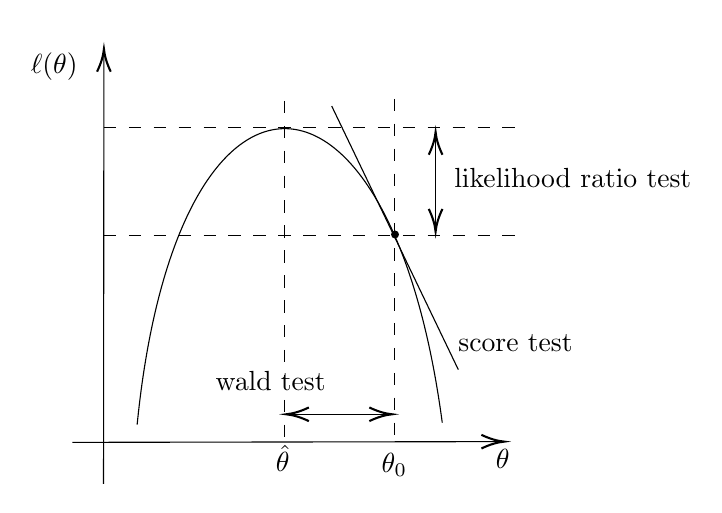
\begin{tikzpicture}[x=0.75pt,y=0.75pt,yscale=-1,xscale=1]
    %uncomment if require: \path (0,300); %set diagram left start at 0, and has height of 300
    
    %Straight Lines [id:da05901855388064847] 
    \draw    (116.28,209.29) -- (322.28,208.93) ;
    \draw [shift={(324.28,208.93)}, rotate = 179.9] [color={rgb, 255:red, 0; green, 0; blue, 0 }  ][line width=0.75]    (10.93,-3.29) .. controls (6.95,-1.4) and (3.31,-0.3) .. (0,0) .. controls (3.31,0.3) and (6.95,1.4) .. (10.93,3.29)   ;
    %Straight Lines [id:da6809814504013212] 
    \draw    (131.28,229.29) -- (131.46,21.76) ;
    \draw [shift={(131.47,19.76)}, rotate = 90.05] [color={rgb, 255:red, 0; green, 0; blue, 0 }  ][line width=0.75]    (10.93,-3.29) .. controls (6.95,-1.4) and (3.31,-0.3) .. (0,0) .. controls (3.31,0.3) and (6.95,1.4) .. (10.93,3.29)   ;
    %Curve Lines [id:da35148800734702434] 
    \draw    (147.47,200.76) .. controls (166.47,9.76) and (269.47,11.76) .. (294.47,199.76) ;
    %Straight Lines [id:da0191225421830008] 
    \draw  [dash pattern={on 4.5pt off 4.5pt}]  (131.47,109.76) -- (331.27,109.76) ;
    %Straight Lines [id:da3881687285855122] 
    \draw  [dash pattern={on 4.5pt off 4.5pt}]  (218.47,44.76) -- (218.47,209.76) ;
    %Straight Lines [id:da9966156097394681] 
    \draw  [dash pattern={on 4.5pt off 4.5pt}]  (271.47,43.76) -- (271.47,208.76) ;
    %Shape: Circle [id:dp6465475156127207] 
    \draw  [fill={rgb, 255:red, 0; green, 0; blue, 0 }  ,fill opacity=1 ] (270.09,109.13) .. controls (270.09,108.23) and (270.82,107.5) .. (271.72,107.5) .. controls (272.62,107.5) and (273.35,108.23) .. (273.35,109.13) .. controls (273.35,110.03) and (272.62,110.76) .. (271.72,110.76) .. controls (270.82,110.76) and (270.09,110.03) .. (270.09,109.13) -- cycle ;
    %Straight Lines [id:da0777384523122382] 
    \draw  [dash pattern={on 4.5pt off 4.5pt}]  (131.47,57.76) -- (331.27,57.76) ;
    %Straight Lines [id:da9382893328394419] 
    \draw    (241.22,47.26) -- (302.22,174.26) ;
    %Straight Lines [id:da5039040124170437] 
    \draw    (221.27,195.76) -- (268.27,195.76) ;
    \draw [shift={(270.27,195.76)}, rotate = 180] [color={rgb, 255:red, 0; green, 0; blue, 0 }  ][line width=0.75]    (10.93,-3.29) .. controls (6.95,-1.4) and (3.31,-0.3) .. (0,0) .. controls (3.31,0.3) and (6.95,1.4) .. (10.93,3.29)   ;
    \draw [shift={(219.27,195.76)}, rotate = 0] [color={rgb, 255:red, 0; green, 0; blue, 0 }  ][line width=0.75]    (10.93,-3.29) .. controls (6.95,-1.4) and (3.31,-0.3) .. (0,0) .. controls (3.31,0.3) and (6.95,1.4) .. (10.93,3.29)   ;
    %Straight Lines [id:da9886798109865442] 
    \draw    (291.27,61.76) -- (291.27,105.76) ;
    \draw [shift={(291.27,107.76)}, rotate = 270] [color={rgb, 255:red, 0; green, 0; blue, 0 }  ][line width=0.75]    (10.93,-3.29) .. controls (6.95,-1.4) and (3.31,-0.3) .. (0,0) .. controls (3.31,0.3) and (6.95,1.4) .. (10.93,3.29)   ;
    \draw [shift={(291.27,59.76)}, rotate = 90] [color={rgb, 255:red, 0; green, 0; blue, 0 }  ][line width=0.75]    (10.93,-3.29) .. controls (6.95,-1.4) and (3.31,-0.3) .. (0,0) .. controls (3.31,0.3) and (6.95,1.4) .. (10.93,3.29)   ;
    
    % Text Node
    \draw (213,209.4) node [anchor=north west][inner sep=0.75pt]    {$\hat{\theta }$};
    % Text Node
    \draw (264,213.4) node [anchor=north west][inner sep=0.75pt]    {$\theta _{0}$};
    % Text Node
    \draw (95,20.4) node [anchor=north west][inner sep=0.75pt]    {$\ell ( \theta )$};
    % Text Node
    \draw (319,211.4) node [anchor=north west][inner sep=0.75pt]    {$\theta $};
    % Text Node
    \draw (301,156) node [anchor=north west][inner sep=0.75pt]   [align=left] {score test};
    % Text Node
    \draw (184,174) node [anchor=north west][inner sep=0.75pt]   [align=left] {wald test};
    % Text Node
    \draw (299,76) node [anchor=north west][inner sep=0.75pt]   [align=left] {likelihood ratio test};
    
    
    \end{tikzpicture}
    \caption{Illustration of Tests on $ \ell(\theta ) $-$ \theta  $ Plot}
    \label{}
\end{figure}



\subsubsection{Non-Parametric Estimation to Survival Function}
In this part we only focus on right censor data $ (\tilde{T}_i,\delta _i) $, $ \delta _i=0 $ for right censoring.

\begin{point}
    Kaplan-Meier Estimator\index{KM Estimator (Kaplan-Meier Estimator)}
\end{point}

Idea of KM Estimator: Separate time into segments by censor/event time $ t_i $, and decompose survival function into products of hazard within segments, using \autoref{EqaSurvivalFunctionDecomposition} which is:
\begin{align}
    \hat{S}(t)=\hat{\mathbb{P}}(T>t)=&\prod_{t_i\leq t}\hat{\mathbb{P}}\left( T>t_i |T>t_{i-1}  \right) \\
    =&\hat{\mathbb{P}}\left( T>t|T>t_i \right)  \prod_{t_i\leq t}\left[1- \hat{\mathbb{P}}\left( t_{i}\geq T>t_{i-1} |T>t_{i-1}\right) \right]\\
    =&\left(1-\hat{\lambda }(t_i)\right)\prod_{t_i\leq t}\left(1-\hat{\lambda }(t_{i-1})\right)\\
    =&\prod_{t_i\leq t}\left[1-\hat{\lambda }(t_i)\right]
\end{align}

where $ \hat{\lambda }(t_i) $ are relatively easy to estimate with censoring considered. $ r_i $ for \# at risk: not censored/event till $ t_i $, $ d_i $ for \# event (death). We can model $ \hat{\lambda }_i $ as
\begin{equation}
    d_i\big|r_i \sim B(r_i,\lambda _i)\xrightarrow[]{\mathscr{L}} N(r_i\lambda _i,r_i\lambda _i(1-\lambda _i))
\end{equation}

and obtain the MLE estimation of $ \hat{\lambda }_i|r_i,d_i $\footnote{Here we use the $ \Delta  $ method for estimating the variance of function of r.v.: if $ X\sim f(\mu ,\sigma ^2) $:
\begin{align}
    g(X)\approx g(\mu )+g'(\mu )(X-\mu )\Rightarrow var(g(X))\approx [g'(\mu )]^2var(X)\leftarrow [g'(X)]^2var(X)
\end{align}}

\begin{align}
    \hat{\lambda }_i=&\dfrac{d_i}{r_i}\\
    var(\hat{\lambda }_i)=&var(\dfrac{d_i}{r_i})=\dfrac{\hat{\lambda }_i(1-\hat{\lambda }_i)}{r_i}\\
    \hat{S}(t)=&\prod_{t_i\leq t}\left[1-\hat{\lambda }(t_i)\right]=\prod_{t_i\leq t}\left[1-\dfrac{d_i}{r_i}\right]\tag{KM Estimator}\\
    var(\hat{S}(t))=&var\left\{ \exp\left[ \log\hat{S(t)} \right] \right\}\\
    \approx&[\hat{S}(t)]^2var\left[\log \hat{S}(t)\right]\\
    =&[\hat{S}(t)]^2\sum_{t_i\leq t}var\left[\log (1-\hat{\lambda }_i) \right]\\
    =&[\hat{S}(t)]^2\sum_{t_i\leq t}\dfrac{1}{(1-\hat{\lambda }_i)^2}var(\hat{\lambda }_i)\\
    =&[\hat{S}(t)]^2\sum_{t_i\leq t}\dfrac{d_i}{r_i(r_i-d_i)}\tag{Greenwood' Formula}\\
    =&[\hat{S}(t)]^2var(\hat{\Lambda }(t))
\end{align}

Interval Estimation of $ \hat{S}(t) $ can be conducted using pointwise interval/confidence band:
\begin{itemize}[topsep=2pt,itemsep=0pt]
    \item Plain pointwise approach:
    \begin{equation}
        \hat{S}(t)\pm N_{1-\frac{\alpha }{2}}\sigma [\hat{S}(t)] 
    \end{equation}
    \item Log-Log pointwise approach (\lstinline|R.| default): using $ \hat{L}(t)=\log\left[-\log \hat{S}(t)\right]=\log\left[\hat{\Lambda }(t)\right] $
    \begin{equation}
         \hat{S}(t)\times e^{\pm N_{1-\frac{\alpha }{2}}\sigma (\hat{L }(t))}
    \end{equation}
    where 
    \begin{equation}
        \sigma (\hat{L }(t))=\sqrt[]{\dfrac{1}{[\log \hat{S}(t)]^2}} \sum_{t_i\leq t}\dfrac{d_i}{r_i(r_i-d_i)}
    \end{equation}
    \item EP confidence band approach
    \item HW confidence band approach
\end{itemize}

Estimator of mean survival time:
\begin{align}
    \hat{\mu }_\tau=&\int _0^\tau \hat{S}(t) \,\mathrm{d}t\\
    var(\hat{\mu }_\tau)=&\sum_{t_i}\left[\int _{t_i}^\tau \hat{S}(t) \,\mathrm{d}t\right]^2\dfrac{d_i}{r_i(r_i-d_i)}
\end{align}
    
\begin{point}
    Nelson-Aalen Estimator\index{NA Estimator (Nelson-Aalen Estimator)}
\end{point}

Idea of NA Estimator: estimate $ \hat{\Lambda }(t) $ first, then obtain Fleming-Harrington Estimator $ \hat{S}_{FH}(t)=e^{-\hat{\Lambda }(t)} $\index{FH Estimator (Fleming-Harrington Estimator)}:
\begin{align}
    \hat{\Lambda }(t)=&\sum_{t_i\leq t}\hat{\lambda }(t_i)=\sum_{t_i\leq t}\dfrac{d_i}{r_i}\\
    var(\hat{\Lambda }(t))=&\sum_{t_i\leq t}\dfrac{d_i(r_i-d_i)}{r_i^2(r_i-1)}\\
    \hat{S}_{FH}(t)=&\exp\left[ -\hat{\Lambda }(t) \right]
\end{align}

\begin{point}
    Survival Function of Life Table
\end{point}

A key difference of survival data of life table is that we cannot know the exact event time/censor time, locating in $ [t_{i-1},t_i) $, in this case we usually estimate $ d_i,\,r_i $ using
\begin{align}
    d_i'=&d_i\\
    r_i'=&r_i-\dfrac{c_i}{2}
\end{align}
where $ c_i $ is \# censor in $ [t_i,t_{i+1}) $, $ r_i $ is \# censoring at the begeinning of interval, i.e. $ t_{i-1} $. And construct KM/NA estimator:
\begin{align}
    \hat{S}_{KM}(t)=&\prod_{t_i\leq t}\left( 1-\dfrac{d_i}{r_i'} \right)\\
    var(\hat{S}_{KM}(t))=&\left[\hat{S}_{KM}(t)\right]^2\sum_{t_i\leq t}\dfrac{d_i}{r_i'(r_i'-d_i)}\\
    \hat{\lambda }(t_{\mathrm{mid\,}i })=&=\dfrac{\hat{f}(t_i)}{\hat{S}(t_i)}= \dfrac{d_i}{(t_{i}-t_{i-1})(r_i'-\frac{d_i}{2})}=\dfrac{d_i}{(t_{i}-t_{i-1})(r_i-\frac{c_i+d_i}{2})}
\end{align}

    where $ \mathrm{mid}\,i  $ means the mid point of $ [t_{i-1},t_{i}) $, i.e. $ \dfrac{t_{i-1}+t_{i}}{2} $


\subsubsection{Hypothesis Testing to Group Comparison}
Key focus: how to judge the difference between two survival function $ S_1(t),\,S_2(t) $, or even when there are more than two groups.

\begin{point}
    Mantel-Haenszel Logrank Test\index{Mantel-Haenszel Logrank Test}
\end{point}\footnote{Note: Log means `time record' here, rather than logarithm.}

Idea of logrank test: adapt contingency table to censor table
\begin{table}[H]
    \centering
    \renewcommand\arraystretch{1}
    \caption{$ 2\times 2 $ contingency table}
    \begin{tabular}{cccc}
        \hline
        \hline
        &\multicolumn{2}{c}{Event $ \delta  $}&\\
        \cline{2-3}
        Group&Yes(1)&No(0)&Total\\
        \hline
        $ 0 $&$ d_0 $&$ r_0-d_0 $&$ r_0 $\\
        $ 1 $&$ d_1 $&$ r_1-d_1 $&$ r_1 $\\
        \hline
        Total&$ d $&$ r-d $&$ r $\\
        \hline
        \hline
    \end{tabular}
    \label{}
\end{table}

\begin{itemize}[topsep=2pt,itemsep=0pt]
    \item Recap: Pearson's $ \chi^2 $ test: assign $ n $ sample into $ k $ groups, and conduct test on $ p_i $, $ i=1,2,\ldots,k $, denote that $ v_i $ samples are assigned to the $ i^\mathrm{th}  $ groups, then
    \begin{equation}
        K_n=\sum_{i=1}^k\dfrac{(v_i-np_i)^2}{np_i}\xrightarrow[]{\mathscr{L}} \chi^2_{df}
    \end{equation}

    In the above example, $ df=k-1 $. In $ 2\times 2 $ contingency table, $ df=1 $ because we assume $ d,r,r_0,r_1 $ are fixed. Pearson's $ \chi^2 $ statistics for $ 2\times 2 $ contingency table:
    \begin{align}
        \chi^2_P=&\sum_{4\text{ grids}}\dfrac{(\mathrm{obs}-\mathrm{expe})^2}{\mathrm{expe} }\\
        =&\dfrac{(d_0-r_0\frac{d}{r})^2}{r_0\frac{d}{r}}+\mathrm{etc}\\
        =&\dfrac{\left[ d_0-r_0\frac{d}{r} \right]^2}{r_0r_1d(r-d)\big/ r^3} \sim \chi^2_1
    \end{align}
    \item Recap: Mental-Haenszel test, based on the Hypergeometric distribution that \index{MH Test (Mental-Haenszel Test)}
    \begin{equation}
        d_0 \sim H(r_0,d,r)\Rightarrow \begin{cases}
            \mathbb{E}\left( d_0 \right)= r_0\dfrac{d}{r}\\
            var(d_0)=\dfrac{r_0r_1d(r-d)}{r^2(r_0-1)}
        \end{cases} ,\quad d_1,r_0-d_0,r_1-d_1 \,\mathrm{similar} 
    \end{equation}

    and construct
    \begin{equation}
        \chi^2_{MH}=\dfrac{\left(\sum_{4\text{ grids}}\mathrm{obs}-\mathbb{E}\left( \mathrm{obs}  \right)\right)^2  }{\sum_{4\text{ grids}} var(\mathrm{obs} )}=\dfrac{\left[ d_0-r_0\frac{d}{r} \right]^2}{\frac{r_0r_1d(r-d)}{r^2(r-1)}}\sim \chi^2_1
    \end{equation}
        
    $ \chi^2_{{MH}} $ and $ \chi^2_{P} $ are equal for lare $ r $.
    \begin{equation}
        \chi^2_{MH}=\dfrac{r-1}{r}\chi^2_P 
    \end{equation}

    \item Cochran-Mantel-Haenszel log-rank test\index{CMH Test (Cochran-Mantel-Haenszel Test)}
    
    For survival data $ t_1,t_2,\ldots,t_K $, we can construct a contingency table $ \mathcal{C}_i $ at each time, and test on the $ K\times 2\times 2 $ contingency table sequence:

    \begin{table}[H]
        \centering
        \renewcommand\arraystretch{1}
        \caption{$ 2\times 2 $ contingency table, $ j=1,2,\ldots,K $}
        \begin{tabular}{cccc}
            \hline
            \hline
            &\multicolumn{2}{c}{Event $ \delta  $}&\\
            \cline{2-3}
            Group&Yes(1)&No(0)&Total\\
            \hline
            $ 0 $&$ d_{0j} $&$ r_{0j}-d_{0j} $&$ r_{0j} $\\
            $ 1 $&$ d_{1j} $&$ r_{1j}-d_{1j} $&$ r_{1j} $\\
            \hline
            Total&$ d_j $&$ r_j-d_j $&$ r_j $\\
            \hline
            \hline
        \end{tabular}
        \label{}
    \end{table}

    and get the CMH statistics for testing $ H_0:\theta _{t_1}=\theta _{t_2}=\ldots =\theta _{t_K} =1$, $ \theta  $ for odds ratio between group 0/1.
    \begin{equation}
        \chi^2 _{CMH}=\dfrac{\left[ \sum_{j=1}^K (d_{0j}-r_{0j}\frac{d_j}{r_j}) \right]^2 }{\sum_{j=1}^K \frac{r_{0j}r_{1j}d_j(r_j-d_j)}{r_j^2(r_j-1)}}\sim \chi^2_1
    \end{equation}

    where the $ K $ contingency tables are treated independent, but they are still ordinal beacuse $ r_{j} $ contains information of history $ d_{t_i<t_j},\, c_{t_i<t_j} $
\end{itemize}

Properties \& Special Cases \& Extension of CMH logrank test:
\begin{itemize}[topsep=2pt,itemsep=0pt]
    \item No tied death $ d_j=1 $:
    \begin{equation}\label{EqaCMHTest}
        \chi^2 _{CMH}=\dfrac{\left[ \sum_{j=1}^K (d_{0j}-r_{0j}\frac{d_j}{r_j}) \right]^2 }{\sum_{j=1}^K \frac{r_{0j}r_{1j}d_j(r_j-d_j)}{r_j^2(r_j-1)}}= \dfrac{\left[ \sum_{j=1}^K (d_{0j}-r_{0j}\frac{d_j}{r_j}) \right]^2 }{\sum_{j=1}^K \frac{r_{0j}r_{1j}}{r_j^2}} \sim \chi^2_1,\quad d_{0j}\in\{0,1\}
    \end{equation}
    \item Intuition of $ \mathrm{obs}-\mathbb{E}\left( \mathrm{obs}  \right)   $:
    \begin{align}
        \mathrm{obs}-\mathbb{E}\left( \mathrm{obs}  \right) \approx& d_{0j}-d_j\dfrac{r_{0j}}{r_{j}}\\
        =&\dfrac{r_{0j}r_{1j}}{r_j}\left(\hat{\lambda }_{0j}-\hat{\lambda }_{1j}\right)
    \end{align}
    \item Attach weight $ w_i\geq 0 $, $ i=1,2,\ldots ,K $ to $ \mathcal{C}_i $:
    \begin{equation}
        \chi^2_{CMH,w}=\dfrac{\left[ \sum_{j=1}^K w_j(d_{0j}-r_{0j}\frac{d_j}{r_j}) \right]^2 }{\sum_{j=1}^K w_j^2\frac{r_{0j}r_{1j}d_j(r_j-d_j)}{r_j^2(r_j-1)}}\sim \chi^2_1
    \end{equation}
    
    bu choosing differnet kinds of weight $ \vec{w} $ we could get variants of CMH test.
    \begin{itemize}[topsep=2pt,itemsep=0pt]
        \item $ w_i=1 $ for log-rank test. Focus more on difference at large $ t $
        \item $ w_i=r_i $ for generalized Wilcoxon rank sum test.  Focus more on difference at small $ t $.
    \end{itemize}
    
    Note: weighted log-rank test should be used when \textbf{no cross}  btw. $ S_1(t) $ and $ S_2(t) $. Kink-of-Weight to choose depends on $ H_1 $.
        
    
\end{itemize}



\begin{point}
    Generalized Wilcoxon Rank Sum Test\index{Wilcoxon Two-Sample Rank Sum Test}
\end{point}

\begin{itemize}[topsep=2pt,itemsep=0pt]
    \item Wilcoxon Two-Sample Rank Sum Test: Knowledge of Wilcoxon two-sample rank sum test see \autoref{SubSectionIntroToNonParametricHypothesisTesting}. Recap: to test the distribution difference of $ \vec{X}=(X_{1},X_{2},\ldots,X_{n})  $ and $ \vec{Y}=(Y_{1},Y_{2},\ldots,Y_{m})  $, we mix them together  and rank as $ \vec{Z}=(Z_{(1)},Z_{(2)},\ldots,Z_{(m+n)})$. Rank of $ X_i $:
    \begin{align}
        R_{i}\equiv &\mathrm{rank}(X_i)\text{ in } \vec{Z},\quad i=1,2,\ldots,n  \\
        R\equiv &\sum_{i=1}^nR_i
    \end{align}
        
    A rank sum statistic to test:
    \begin{align}
        &\dfrac{R-\mathbb{E}\left( R \right)}{\sqrt[]{var(R)}}\sim N(0,1)\\
        &\begin{cases}
            \mathbb{E}\left( R \right) =\dfrac{n(m+n+1)}{2}\\
            var(R)=\dfrac{mn(m+n+1)}{12}
        \end{cases}
    \end{align}

    Rank sum statistic can be written in a Mann-Whitney form that can be generalized:\index{Mann-Whitney Form}
    \begin{align}
        U_{ij}=&U(X_i,Y_j)\equiv\begin{cases}
            +1&,\text{case } X_i>Y_j\\
            0&,\text{case } X_i=Y_j\\
            -1&,\text{case }X_i<Y_j
        \end{cases},\qquad U=\sum_{i,j}^{n,m}U_{ij}\\
        R=&\dfrac{n(m+n+1)}{2}+\dfrac{U}{2}
    \end{align}

\item Mann-Whitney-Wilcoxon rank sum test for censored data: 

    Notation: we still mix $ X=\{(\tilde{t}_{1i},\delta _{1i})\}_{i=1}^n $ and $ Y=\{(\tilde{t}_{2j},\delta _{2j})\}_{j=1}^m $ to get:
    \begin{equation}
        Z_\mathrm{mix}=\left\{ (\tilde{t}_i,\delta _i) \right\}_{i=1}^{m+n}  
    \end{equation}
    and the Mann-Whitney form for $ Z_\mathrm{mix}  $:
    \begin{align}
        U_{ij}=&U(Z_i,Z_j)  \equiv\begin{cases}
            +1&,\text{case } \tilde{t}_i>\tilde{t}_j,\, \delta _j=1\\
            0&,\text{case }  \tilde{t}_i=\tilde{t}_j \text{ or } \delta _j=0\\
            -1&,\text{case } \tilde{t}_i<\tilde{t}_j,\, \delta _j=1
        \end{cases},\quad i=1,2,\ldots ,m+n.\, j=1,2,\ldots ,m+n.
    \end{align}
         
    and the Extended Wilcoxon rank sum statistic:
    \begin{equation}
         W=\sum_{i\text{ if }Z_i\in X}^{m+n}\sum_{j=1}^{m+n}U_{ij}
    \end{equation}

    Under $ H_0: X\sim Y $, distribution features
    \begin{align}
        \mathbb{E}\left( W \right) =&0\\
        \hat{var}(W)=&\dfrac{mn}{(m+n)(m+n-1)}\sum_{i=1}^{m+n}\left(\sum_{j=1}^{m+n}U_{ij}\right)^2
    \end{align}

    \begin{itemize}[topsep=2pt,itemsep=0pt]
        \item choose $ w_i=r_i $ in weighted log-rank test, and nominator becomes
        \begin{align}
            \sum_{j=1}^Kr_j(d_{0j}-r_{0j}\dfrac{d_j}{r_j})=&\sum_{j=1}^K\left[ (r_{1j}-d_{1j})d_{0j}-(r_{0j}-d_{0j})d_{1j} \right]\\
            =&\sum_{j=1}^K\left[ \#_{Y>t_j}\times \#_{X=t_j}-\#_{X>t_j}\times \#_{Y=t_j}  \right]\\
            =&\#_{Y>X}-\#_{Y<X}\\
            =&-W
        \end{align}
        in which $ \chi^2_{w_i=r_i,CMH} $ test is the same as generalized Wilcoxon rank sum test.
        
        
    \end{itemize}
    
        
\end{itemize}

\subsection{Survival Model with Covariants} 

To research on the dependence of $ T $ with regard to covariants $ z $. Survival data with covariants: $ X=(\tilde{t}_i,\delta _i,z_i) $

\subsubsection{Cox's Proportion Hazard Model}
Basic assumption on dependence form: $ T $ hazard part and covariants part are Separatable:\index{PH Model (Cox's Proportion Hazard Model)}
\begin{equation}
    \lambda (t|z)=\lambda _0(t)g(z)\Leftrightarrow S(t|z)=\left[S_0(t)\right]^{g(z)},\quad S_0(t)=e^{-\int _0^t\lambda _0(\tau) \,\mathrm{d}\tau}
\end{equation}

further a linear form $ g(z)=\beta ^Tz $ is used;
\begin{equation}
     \lambda (t|z)=\lambda _0(t)\exp\left[ \beta ^Tz \right]
\end{equation}

Basic Assumptions of Cox's PH Model:
\begin{itemize}[topsep=2pt,itemsep=0pt]
    \item constant regression coefficient $ \beta  $;
    \item linear dependent of covariants $ \beta 'z $;
    \item exponential link function $ e^\cdot $
\end{itemize}

    

in this proportion hazard model, the ratio of hazard only depend on $ \beta  $:
\begin{equation}
    \log\left\{ \dfrac{\lambda _{z_i}(t)}{\lambda _0(t)} \right\}=\beta ^Tz_i\parallel t 
\end{equation}

The unknown components are $ \lambda _0(t),\beta  $, where the $ \lambda _0(t) $ lies in the $ dim\to\infty $ space, and causes difficulty in conducting inference. Solution: decompose full likelihood into two parts, in which one of them, \textbf{Partial Likelihood} is only function of $ \beta  $:\index{Partial Likelihood}
\begin{align}
    L(\beta ,\lambda _0(\cdot);X)=&\prod_{i}\left[ \left( \lambda _0(t_i)e^{\beta ^Tz_i} \right)^\delta _i\left( e^{-\int _{0}^{t_i}\lambda _0(\tau) \,\mathrm{d}\tau} \right)^{e^{\beta ^Tz_i}} \right]\\
    =&L_{PH}(\beta ;X)L_{res}(\beta ,\lambda _0;X)
\end{align}

and we could focus on $ L_{PH} $ for further inference.

Note: the feasibility of partial likelihood comes from the form of proportion hazard.

\begin{point}
    Partial Likelihood without Tie
\end{point}

\textit{Derivation:} First we assert $ t_i $ in ascending order and without tie: $ t_1<t_2<\ldots <t_n $, and we use an discrete estimated form of $ \lambda _0(t_i)=\lambda _i $
\begin{equation}
    \int _0^{t_i}\lambda _0(\tau) \,\mathrm{d}\tau \approx \sum_{j=1}^i\lambda _j
\end{equation}
then we could use a trick to reformulate $ \ell(\beta ,\lambda _1,\ldots,\lambda _n;X) $ as\footnote{\newcommand{\blue}{\color{blue}}\newcommand{\brown}{\color{brown}}
Illustration for $ \blue\displaystyle\sum_{i=1}^n\lambda _i\sum_{j=i}^ne^{\beta 'z_j}=\sum_{i=1}^n\sum_{j=1}^i\lambda _je^{\beta 'z_i} $
\begin{equation}\begin{pNiceMatrix}[last-row,last-col,nullify-dots,xdots/line-style={dashed,blue}]

\lambda _1e^{\beta 'z_1}&&&&&\brown\leftarrow\sum_{j=1}^1\lambda _je^{\beta 'z_1}\\
\lambda _1e^{\beta 'z_2}&\lambda _2e^{\beta 'z_2}&&&&\brown\leftarrow\sum_{j=1}^2\lambda _je^{\beta 'z_2}\\
\lambda _1e^{\beta 'z_3}&\lambda _2e^{\beta 'z_3}&\lambda _3e^{\beta 'z_3}&&&\brown\leftarrow\sum_{j=1}^3\lambda _je^{\beta 'z_3}  \\
\vdots&\vdots&\vdots&\ddots&&\brown\leftarrow\vdots\\
\lambda _1e^{\beta 'z_n}&\lambda _2e^{\beta 'z_n}&\lambda _3e^{\beta 'z_n}&\cdots&\lambda _ne^{\beta 'z_n}&\brown\leftarrow\sum_{j=1}^n\lambda _je^{\beta 'z_n}\\
\brown\overset{\uparrow}{\lambda _1\sum_{j=1}^ne^{\beta 'z_j}}&\brown\overset{\uparrow}{\lambda _2\sum_{j=2}^ne^{\beta 'z_j}}&\brown\overset{\uparrow}{\lambda _3\sum_{j=3}^ne^{\beta 'z_j}}&\brown\overset{\uparrow}{\cdots}&\brown\overset{\uparrow}{\lambda _n\sum_{j=n}^ne^{\beta 'z_j}}&\blue\sum_{i=1}^n\lambda _i\sum_{j=i}^ne^{\beta 'z_j}=\sum_{i=1}^n\sum_{j=1}^i\lambda _je^{\beta 'z_i}
\end{pNiceMatrix}\end{equation}
}

\begin{align}
    \ell(\beta ,\lambda _1,\ldots,\lambda _n)=&\sum_{i=1}^n\left\{ \delta _i(\log\lambda _i+\beta 'z_i)-{\color{blue}\sum_{j=1}^i\lambda _je^{\beta 'z_i}} \right\}\\
    =&\sum_{i=1}^n\left\{ \delta _i(\log\lambda _i+\beta 'z_i)-{\color{blue}\lambda _i\sum_{j=i}^ne^{\beta 'z_j}} \right\}
\end{align}

and use MLE with regard to $ \lambda _i $ to get an estimate to $ \lambda _i $: 
\begin{equation}
    \dfrac{\partial^{} \ell(\beta ,\lambda _1,\ldots,\lambda _n)}{\partial \lambda _i^{}}=0\Rightarrow \lambda _i(\beta )=\dfrac{\delta _i}{\sum_{j=1}^ne^{\beta 'z_j}} \quad \forall i
\end{equation}

then we could get the partial likelihood
\begin{align}
    L(\beta ,\lambda _1(\beta ),\ldots,\lambda _n(\beta ))=&\prod_{i=1}^n\lambda _i(\beta )^{\delta _i}e^{\delta _i\beta 'z_i}e^{-\sum_{j=1}^ne^{\beta 'z_i}}\\
    =&e^{-\sum_i\delta _i}\prod_{i=1}^n\left( \dfrac{e^{\beta 'z_i}}{\sum_{j:t_j\geq t_i}e^{\beta 'z_j}} \right)^{\delta _i}\\
    PL(\beta )\equiv&\prod_{i=1}^n\left( \dfrac{e^{\beta 'z_i}}{\sum_{j:t_j\geq t_i}e^{\beta 'z_j}} \right)^{\delta_i}\\
    P\ell=&\sum_{i=1}^n\delta _i\left[ \beta 'z_i-\log\left(\sum_{j:t_j\geq t_i}e^{\beta 'z_j}\right) \right]\\
    U(\beta )=&\sum_{i=1}^n\delta _i\left[ z_i-\dfrac{\sum_{j:t_j\geq t_i}z_je^{\beta 'z_j}}{\sum_{j:t_j\geq t_i}e^{\beta 'z_j}} \right]\\
    J(\beta )=&\sum_{i=1}^n\delta _i\left[ \sum_{j:t_j\geq t_i}^n \dfrac{e^{\beta 'z_j}}{\sum_{l:t_l\geq t_j}e^{\beta 'z_l}} \left( z_j-\dfrac{\sum_{l:t_l\geq t_j}z_le^{\beta 'z_l}}{\sum_{l:t_l\geq t_j}e^{\beta 'z_l}} \right)^2 \right]
\end{align}

The above statistics can be use for further inference.
\begin{align}
    &J(\beta _0)^{-1/2}U(\beta _0)\xrightarrow[]{\mathscr{L}} N(0,1)\\
    &(\hat{\beta }-\beta _0)\xrightarrow[]{\mathscr{L}} N(0,J(\hat{\beta })^{-1})\\
    &2(\ell(\hat{\beta })-\ell(\beta))\xrightarrow[]{\mathscr{L}} \chi^2_p
\end{align}

\begin{point}
    Modification for Partial Likelihood with Tie
\end{point}

There are various modification for tied data case. In PL without tie, the $ \dfrac{e^{\beta 'z_i}}{\sum_{j:t_j\geq t_i}e^{\beta 'z_j}} $ term are usually changed to adapt for the case of. Intuition:
\begin{equation}
    \dfrac{e^{\beta 'z_i}}{\sum_{j:t_j\geq t_i}e^{\beta 'z_j}}=\dfrac{\lambda (t_i|z_i)}{\sum_{j:t_j\geq t_i}\lambda (t_j|z_j)}\approx \mathbb{P}\left( i^\mathrm{th} \text{event}|1\text{out of }\# \{j:t_j\geq t_i\}  \right) 
\end{equation}

Notation: $\mathcal{R}_i $ for all datapoints at risk at time $ t_i $, $ \mathcal{D}_i $ for event cases at time $ t_i $, $ \mathcal{D}_i\subset \mathcal{R}_i $
\begin{itemize}[topsep=2pt,itemsep=0pt]
    \item Cox's modification:\indexname{Cox's Modification}
    \begin{equation}
        \mathbb{P}\left( \mathcal{D}_i \text{ events}\Big| |\mathcal{D}_i |\text{out of }\# \{j:t_j\geq t_i\}  \right)=\dfrac{e^{\sum_{l\in\mathcal{D}_i }\beta'z_l }}{\sum_{\text{all possible }|\mathcal{D}_j|=|\mathcal{D}_i | }e^{\sum_{l\in\mathcal{D}_j }\beta'z_j} }
    \end{equation}
    drawback: $ \sim O(|\mathcal{D}_i|!) $ complexity
    \begin{align}
        PL(\beta )=&\prod_{i=1}^n\left\{ \dfrac{e^{\sum_{l\in\mathcal{D}_i}\beta 'z_l}}{\sum_{\text{all possible }|\mathcal{D}_j|=|\mathcal{D}_i|}e^{\sum_{l\in\mathcal{D}_j}}e^{\sum_{l}\in\mathcal{D}_j}\beta 'z_l} \right\} 
    \end{align}
    
    
    \item Breslow's approximation:\index{Breslow's Approximation}
    \begin{equation}
        \mathbb{P}\left( \mathcal{D}_i \text{event}\Big| |\mathcal{D}_i |\text{out of }\# \{j:t_j\geq t_i\}  \right)\approx \dfrac{e^{\sum_{l\in\mathcal{D}_i }\beta'z_l }}{\left(\sum_{l\in\mathcal{R}_i}e^{\beta 'z_l}\right)^{|\mathcal{D}_i|}}
    \end{equation}
    or directly write the PL as
    \begin{equation}
        PL(\beta )=\prod_{i=1}^n \left\{ \prod_{j\in\mathcal{D}_i}\dfrac{e^{\beta 'z_j}}{\sum_{l\in\mathcal{R}_i}e^{\beta 'z_l}} \right\}
    \end{equation}
    \item Efron's approximation: usually better than Breslow's, default method in \lstinline|coxph()|\index{Efron's Approximation}
    \begin{align}
        PL(\beta )=\prod_{i=1}^n\left\{ \dfrac{e^{\sum_{l\in\mathcal{D}_i}\beta 'z_l}}{ \prod_{j=1}^{|\mathcal{D}_i|}\left( \sum_{l\in\mathcal{R}_i}e^{\beta 'z_l}-\frac{j-1}{|\mathcal{D}_i|}\sum_{l\in\mathcal{D}_i}e^{\beta 'z_l} \right) } \right\} 
    \end{align}
    
    
\end{itemize}


\begin{point}
    Extension for Time-Dependent Variable
\end{point}

Model:
\begin{align}
    \begin{cases}
        \lambda (t)=&\lambda _0(t)e^{\beta 'z(t)}\\
        \lambda (t)=&\lambda _0(t)e^{\beta (t) 'z}
    \end{cases}
\end{align}

\begin{point}
    Diagnostic Methods for PH Assumption
\end{point}

\begin{itemize}[topsep=2pt,itemsep=0pt]
    \item $ \log $-$ \log $ plots: for categorical $ z_1 $, $ z_2 $, use relation
    \begin{align}
        \log\left[-\log S(t,z_1)\right] -\log\left[-\log S(t,z_2)\right] =\beta '(z_1-z_2)\independent t
    \end{align}
    
    Plot of $ \log\left[\log \hat{S}(t,z)\right] $ should be 'parallel' curves.
    
    \item Check the coherence bet. observed data v.s. expected data.
    \item Goodness-of-fit using Schoenfeld residuals\indexname{Schoenfeld Residual}
    \begin{align}
        \hat{r}_i=&z_i-\sum_{j\in\mathcal{R}_i}z_k\cdot p(\hat{\beta },z_k)=z_i\bar{z}_i\\
        p(\beta ,z_k):=&\dfrac{e^{\beta 'z_k}}{\sum_{j\in\mathcal{R}_k}e^{\beta 'z_j}} 
    \end{align}
    \item (Generalized) Cox-Snell Residual for overall goodness-of-fit: \index{Cox-Snell Residual}
    
    Recall: for r.v. $ T\sim f(t) $, $ S(t)=\int _t^\infty f(\tau) \,\mathrm{d}\tau $. function of r.v. has distribution:
    \begin{align}
        S(T)\sim U(0,1)\Rightarrow \Lambda (T)\sim \varepsilon (1) 
    \end{align}

    define Cox-Snell Residual:
    \begin{align}
        \hat{\Lambda }(z_i)=-\log \hat{S}(z_i) 
    \end{align}

    the set $ \{\hat{\Lambda }(z_i)\} $ could be viewed as a sample from $ \varepsilon (1) $, we could test on the distribution, e.g. plot the cumulative hazard \textbf{of residual} v.s. residual to check $ \Lambda (e)=e $.
    
    \item Delta-Beta Residual for infulential: \index{Delta-Beta Residual} for $ \beta =(\beta _0=1,\beta _1,\ldots) $, define
    \begin{align}
        \hat{\Delta }_{ij}=\hat{\beta }_j-\hat{\beta }_{j(\wedge i)} 
    \end{align}

    where $ \wedge i $ for estimator with the $ i^\mathrm{th}  $ subject removed. Plot the scatter plot of $ \hat{\Delta }_{ij} $ to locate influential.

    % \item Martingale Residual for non-linearity: \index{Martingale Residual}
\end{itemize}

\begin{point}
    Experiment Design for Log-rank Test under PH Assumption
\end{point}

    Question: how many events are needed for the testing $ H_0:\beta =0\leftrightsquigarrow H_a:\beta =\beta _a $?

    Using log-rank statistics \autoref{EqaCMHTest} in $ z $-test form, under condition 1. no ties $ d_j=0,1 $, 2. $ \beta _a $ is small enough for taylor expansion:\footnote{Proof key: 
    \begin{align}
        d_{0j}\sim B(p_{0j}), \quad  p_{0j}=\dfrac{r_{0j}\lambda _0}{r_{0j}\lambda _0+r_{1j}\lambda _0e^{\beta _a} }
    \end{align}
    
    and at small $ \beta _a $, take approximation $ \theta \approx r_{1j}/r_{j} $
    }
    \begin{align}
        T_{CMH}= \dfrac{\sum_{j=1}^K\left( d_{0j}-r_{oj}\frac{d_j}{r_j} \right)}{\sqrt[]{\sum_{j=1}^K}\frac{r_{0j}r_{1j}d_j(r_j-d_j)}{r_j^2(r_j-1)}}\xrightarrow[]{\mathscr{L}} N(\beta _a\sqrt[]{d\theta (1-\theta )}, 1)
    \end{align}

    where $ d=\sum_{j=1}d_j $, $ \theta  $ is the prevalence of group 1.

    Power of the test: denote $ \gamma  $ for probability of type II error
    \begin{align}
        \mathbb{P}\left( T_{CMH}>N_{\alpha /2}|H_a \right) = 1-\gamma \Rightarrow \mu :=\beta _a\sqrt[]{d\theta (1-\theta )}\approx N_{\alpha /2}+N_\gamma 
    \end{align}

    Minimum number of events:
    \begin{align}
        d=\dfrac{(N_{\alpha /2}+N_\gamma )^2}{\beta _a^2\theta (1-\theta )} 
    \end{align}
    
    
    
    
    
    

    

\subsubsection{Accelerated Failure Time Model}

    Basic form of AFT Model (Accelerated Failure Tome Model)\index{AFT Model (Accelerated Failure Tome Model)} for categorical covariants:
    \begin{align}
        S(t;z=1)=S(\gamma t;z=2)\Leftrightarrow \mathbb{P}\left( T_1>t \right) =\mathbb{P}\left( T_2>\gamma t \right)  
    \end{align}

    Usually we attach some assumptions on function form of $ S(t,z) $, usually take (parameter denoted $ \alpha  $):
\begin{itemize}[topsep=2pt,itemsep=0pt]
    \item Exponential:
    \begin{align}
        S(t)=&e^{-\lambda t},\quad \lambda (t)=\lambda \\
        \Rightarrow &t=-\dfrac{1}{\lambda }\log S(t)\\
        \Rightarrow &\gamma :=e^{\alpha 'z}=\dfrac{1}{\lambda }=e^{-\beta 'z}
    \end{align}

    i.e. Exponential AFT model in which $ \gamma =e^{\alpha 'z} $ is equivalent to PH model with $ \lambda =e^{\beta 'z} $, and $ \beta =-\alpha  $ 
    
    \item Weibull:
    \begin{align}
        S(t)=&e^{-\lambda t^p},\quad \lambda (t)=\lambda pt^{p-1}\\
        \Rightarrow &t=-\dfrac{1}{\lambda ^{1/p}}\log S(t)\\
        \Rightarrow &\gamma :=e^{\alpha 'z}=\dfrac{1}{\lambda ^{1/p}}=e^{-\beta 'z/p}
    \end{align}
    
    i.e. Weibull AFT model with $ \gamma =e^{\alpha 'z} $ is equivalent to PH model with $ \lambda =e^{\beta 'z} $, and $ \beta =-\alpha p $
    
    \item General Case: In different groups $ z $, survivial time 
    \begin{align}
        T_i=&T_0e^{\alpha 'z_i+ \varepsilon _i/p },\quad \varepsilon _i\sim \varepsilon (1)
        S_i(t)=&\mathbb{P}\left( T_i\geq t \right)\\
        =&\mathbb{P}\left( \log T_0 +\alpha 'z_i+\dfrac{\varepsilon _i}{p}\geq  \log t \right)  \\
        =&S_{\varepsilon (1)}\left(p({\log t-\log T_0-\alpha 'z_i})\right)
    \end{align}
    
    
    
    
\end{itemize}


\begin{point}
    AFT Model and PH Model
\end{point}

    An intuition for parameters in AFT model and PH model:
\begin{figure}[H]
    \centering
    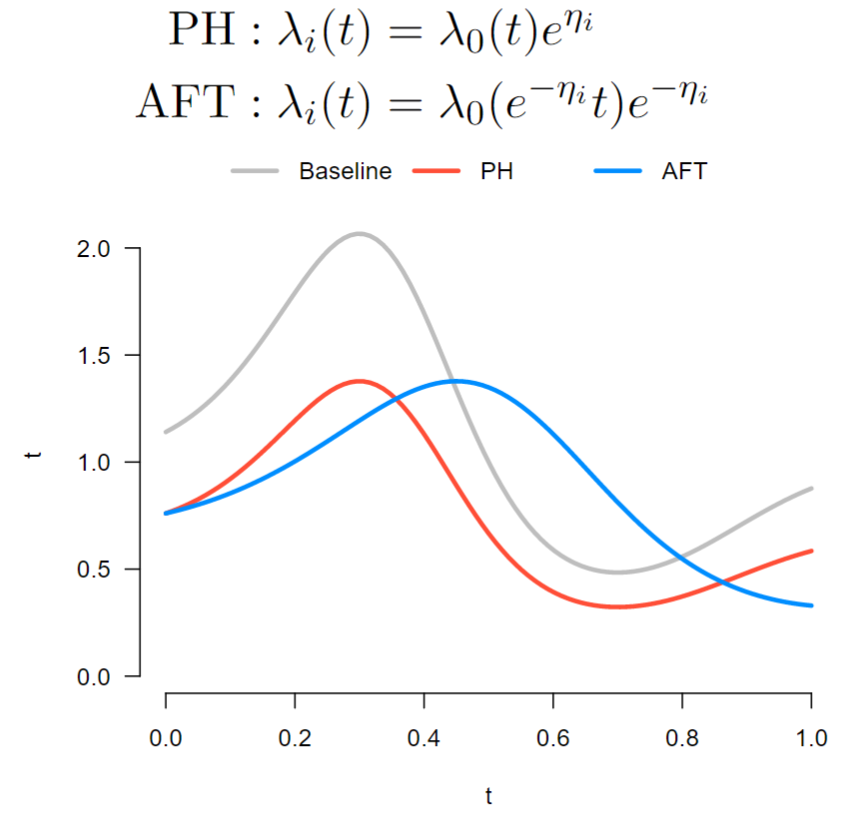
\includegraphics[width=0.45\linewidth]{sections/images/2022-08-19-10-03-10.png}
    \label{}
\end{figure}

    Usually AFT model depends on a parametric model, whlie PH model only depends on the PH assumption.



\begin{rcode}
    An example:
\begin{lstlisting}[language=R]
coxph(formula = Surv(start, stop, event) ~ rx + number + size + factor(enum), data = bladder2)
\end{lstlisting}
\end{rcode}
    
    


    

\newpage

\section{生物统计学概论部分}
\begin{center}
    Instructor: Tianying Wang
\end{center}

Biostatistics is discipline to apply statistical methods to biological problems, including medicine, biology experiment, public health, etc. This section would focus on basic quantative skills to be used in advanced biostatistics research.


\subsection{Factor Model and ANOVA}
\index{Factor Model}\index{ANOVA (Analysis of Variance)}
A major question in biostatistics is to study the difference between groups, i.e. explanatory variable $ X $ is categorical. A `way' to conduct grouping is called a \textbf{factor} , e.g. $ \{\alpha _i\} $ where each $ i $ correponds to a \textbf{level} of the factor.  

To compare groups, e.g. to determine whether there is significant difference between $ Y $ of each group, ANOVA is used. The key thought is to analyze difference value and variance and see whether the difference is large enough to `exceed' variance.

\begin{point}
    Factor Notation
\end{point}

    Response $ Y $ is denoted by its subsript to declare its group and index in this group, e.g. $ Y_{ijkl} $ indicates it is the $ l^\mathrm{th}  $ sample in group $ (i,j,k) $

\subsubsection{Single Factor Model and One-Way ANOVA}
% \index{Factor Model!Single Factor Model}

\begin{point}
    Cell Mean Model
\end{point}

\[
    Y_{ij}=\mu_i +\varepsilon _{ij},\quad \varepsilon _{ij} \,\mathrm{i.i.d.}\,\sim N(0,\sigma ^2) 
\]

Estimation target: $ \mu _1,\ldots,\mu _r,\sigma ^2 $

Hypothesis testing $ H_0 $: $ \mu _1=\ldots=\mu _r=\mu  $, v.s. $ H_1: $ at least 1 $ \mu _i $ is different.

Estimation:
\begin{align}
    \hat{\mu }_i=&\bar{Y}_{i\cdot}=\dfrac{1}{n_i}\sum_{j=1}^{n_i}Y_{ij}\\
    s_i^2=&\dfrac{1}{n_i-1}\sum_{j=1}^{n_i}(Y_{ij}-\bar{Y}_{i\cdot})^2\\
    s^2=&\dfrac{\sum_{i=1}^r(n_i-1)s_i^2}{\sum_{i=1}^r(n_i-1)}=\dfrac{\sum_{i=1}^r(n_i-1)s_i^2}{n_T-r}
\end{align}

Key of ANOVA: Decomposition of variation SS:
\begin{align}
    \mathrm{SST}=  \sum_{i=1}^r\sum_{j=1}^{n_i}(Y_{ij}-\bar{Y}_{\cdot\cdot})^2=&\sum_{i=1}^r\sum_{j=1}^{n_i}\left( Y_{ij}-\bar{Y}_{i\cdot}+\bar{Y}_{i\cdot}-\bar{Y}_{\cdot\cdot} \right)^2\\
    =&\sum_{i=1}^{r}+\sum_{j=1}^{n_i}(Y_{ij}-\bar{Y}_{i\cdot})^2+\sum_{i=1}^r(\bar{Y}_{i\cdot}-\bar{Y}_{\cdot\cdot})^2\\
    =&\mathrm{SSE}+\mathrm{SSR}  
\end{align}

\begin{point}
    Factor Model
\end{point}

    
    \begin{align}
        Y_{ij}=\mu+\alpha _i+\varepsilon _{ij}\quad \varepsilon _{ij}\text{ i.i.d. }\sim N(0,\sigma ^2) 
    \end{align}    

    Estimation target: $ \mu ,\alpha _1,\ldots,\alpha _r,\sigma ^2 $, w.r.t. $\sum_{i=1}^r\alpha _i=0$.

    Hypothesis tesing: $ H_0:\,\alpha _1=\ldots=\alpha _r=0 $, v.s. $ H_1: $ at least 1 $ \alpha _i\neq 0 $

    Estimation:
    \begin{align}
        \hat{\mu }=&\bar{Y}_{i\cdot }=\dfrac{1}{n_i}\sum_{j=1}^{n_i}Y_{ij}\\
        s_i^2=&\dfrac{1}{n_i-1}\sum_{j=1}^{n_i}\left(Y_{ij}-\bar{Y}_{i\cdot     }\right)^2\\
        s^2=&\dfrac{\sum_{i=1}^r(n_i-1)s_i^2}{n_T-r}
\end{align}    
    
    


\subsubsection{Fixed Effect and Random Effect}
    When divided into groups/naturally assigned in groups, we need to specify whether the factor levels are specially chosen (fixed effect) of randomly chosen from a `population of levels' (random effect). 
    \begin{itemize}[topsep=2pt,itemsep=0pt]
        \item Fixed Effect: whether there is a difference between / estimating the value of mean value $ \mu _i $ of each specific levels
        \item Random Effect: whether the overall behaviour of $ \mu _i $ comes from a `random distribution'
    \end{itemize}

    Comment on fised / random in actual model building and statistical inference:
    \begin{itemize}[topsep=2pt,itemsep=0pt]
        \item whether a factor is fixed or random should be determined by how the data are obtained and the research problem to be studied, i.e. determining fixed / random model does \textbf{not} come from mathematics.
        \item for effect of interaction term, say $ (\alpha\beta )_{ij} $ as the interaction effect of factor $ \alpha _i $ and $ \beta _j $, then $ (\alpha \beta )_{ij} $ would be random once one of $ \alpha _i $ or $ \beta  _j$ is random.
    \end{itemize}
    

    Here use a one-way factor model as example:
    

    \begin{point}
        Fixed Effect:
    \end{point}
    
        
    \begin{align}
        Y_{ij}=\mu+\alpha _i+\varepsilon _{ij}\quad \varepsilon _{ij}\text{ i.i.d. }\sim N(0,\sigma ^2) 
    \end{align}    

    Estimation target: $ \mu ,\alpha _1,\ldots,\alpha _r,\sigma ^2 $, w.r.t. $\sum_{i=1}^r\alpha _i=0$.

    Hypothesis tesing: $ H_0:\,\alpha _1=\ldots=\alpha _r=0 $, v.s. $ H_1: $ at least 1 $ \alpha _i\neq 0 $

    Estimation:
    \begin{align}
        \hat{\mu }=&\bar{Y}_{i\cdot }=\dfrac{1}{n_i}\sum_{j=1}^{n_i}Y_{ij}\\
        s_i^2=&\dfrac{1}{n_i-1}\sum_{j=1}^{n_i}\left(Y_{ij}-\bar{Y}_{i\cdot     }\right)^2\\
        s^2=&\dfrac{\sum_{i=1}^r(n_i-1)s_i^2}{n_T-r}
\end{align}    

    ANOVA table:
    \begin{table}[H]
        \centering
        \renewcommand\arraystretch{1.15}
        \begin{tabular}{cllll}
            \hline
            Source of Var&$ \mathrm{SS} $&$ dof $&$ \mathrm{MS}  $&$ \mathbb{E}\left( \mathrm{MS}  \right)  $\\
            \hline
            $ \alpha _i $&$ \mathrm{SS}\alpha=\sum_{i=1}^rn_i\left(\bar{Y}_{i\cdot }-\bar{Y}_{\cdot \cdot }\right)^2  $&$ r-1 $&$ \dfrac{\mathrm{SS}\alpha  }{r-1} $&$ \sigma ^2+\dfrac{\sum_{i=1}^rn_i\alpha _i^2}{r-1} $\\
            $ \sigma ^2$&$ \mathrm{SSE} =\sum_{i=1}^r\sum_{j=1}^{n_i}\left(Y_{ij}-Y_{i\cdot }\right)^2 $&$ n_T-r $&$ \dfrac{\mathrm{SSE}}{n_T-r} $&$ \sigma ^2 $\\
            \hline
        \end{tabular}
        \caption{}
        \label{}
    \end{table}

    $ F $ statistics for $ H_0:\alpha _1=\ldots=\alpha _r=0 $:
    \begin{align}
        F=\dfrac{\mathrm{MS}\alpha }{\mathrm{MSE} } \sim F_{r-1,n_T-r}
    \end{align}
    
    
    
    

\begin{point}
    Random Effect
\end{point}

\begin{align}
    Y_{ij}=\mu+\alpha _i+\varepsilon _{ij}\quad \alpha _i\text{ i.i.d. }\sim N(0,\sigma _\alpha ^2),\quad \varepsilon _{ij}\text{ i.i.d. }\sim N(0,\sigma ^2) 
\end{align}


    Estimation target: $ \mu ,\sigma _\alpha ^2,\sigma ^2 $

    Hypothesis testing $ H_0:\,\sigma _\alpha ^2=0$, v.s. $ H_1: \sigma _\alpha ^2\neq 0$

    Estimation:
    \begin{align}
        \hat{\mu }=&\bar{Y}_{i\cdot }=\dfrac{1}{n_i}\sum_{j=1}^{n_i}Y_{ij}\\
        s_i^2=&\dfrac{1}{n_i-1}\sum_{j=1}^{n_i}\left(Y_{ij}-\bar{Y}_{i\cdot     }\right)^2\\
        s^2=&\dfrac{\sum_{i=1}^r(n_i-1)s_i^2}{n_T-r}
\end{align}

    ANOVA table:
    \begin{table}[H]
        \centering
        \renewcommand\arraystretch{1.15}
        \begin{tabular}{cllll}
            \hline
            Source of Var&$ \mathrm{SS} $&$ dof $&$ \mathrm{MS}  $&$ \mathbb{E}\left( \mathrm{MS}  \right)  $\\
            \hline
            $ \alpha _i $&$ \mathrm{SS}\alpha=\sum_{i=1}^rn_i\left(\bar{Y}_{i\cdot }-\bar{Y}_{\cdot \cdot }\right)^2  $&$ r-1 $&$ \dfrac{\mathrm{SS}\alpha  }{r-1} $&$ \sigma ^2+n\sigma _\alpha ^2 $\\
            $ \sigma ^2$&$ \mathrm{SSE} =\sum_{i=1}^r\sum_{j=1}^{n_i}\left(Y_{ij}-Y_{i\cdot }\right)^2 $&$ n_T-r $&$ \dfrac{\mathrm{SSE}}{n_T-r} $&$ \sigma ^2 $\\
            \hline
        \end{tabular}
        \caption{}
        \label{}
    \end{table}

    $ F $ statistics for $ H_0:\alpha _1=\ldots=\alpha _r=0 $:
    \begin{align}
        F=\dfrac{\mathrm{MS}\alpha }{\mathrm{MSE} } \sim F_{r-1,n_T-r}
    \end{align}




\subsubsection{Two Factor Model and Two-Way ANOVA}

Two factor model with interation term:

\[
    Y_{ijk}=\mu +\alpha _i+\beta _j+(\alpha \beta )_{ij}+\varepsilon _{ijk} 
\]
% \footnote{When we first introduced double factor model, we expressed interaction term as 
% \begin{align}
%     Y_{ijk} =& \mu +\alpha _i +\beta _j+(\alpha \beta ) _{ij}+\varepsilon _{ijk}
% \end{align}



% }
\begin{align}
    Y_{ijk}-\bar{Y}_{\cdot \cdot \cdot }=&\left(\bar{Y}_{i\cdot \cdot}-\bar{Y}_{\cdot \cdot \cdot}\right)+\left(\bar{Y}_{\cdot j\cdot }-\bar{Y}_{\cdot \cdot \cdot }\right)\\
    &+\left(\bar{Y}_{ij\cdot }-\bar{Y}_{i\cdot \cdot }-\bar{Y}_{\cdot j\cdot }+\bar{Y}_{\cdot \cdot \cdot }\right)+  \left( Y_{ijk}-\bar{Y}_{ij\cdot}\right)\\
    \alpha _i+\beta _j+(\alpha \beta )_{ij}+\varepsilon _{ijk}=&\left((\mu +\alpha _i)-\mu \right)+\left((\mu +\beta _j)-\mu \right)\\
    &+\left( (\mu +\alpha _i+\beta _j+(\alpha \beta )_{ij})-(\mu +\alpha _i)-(\mu +\beta _j)+\mu  \right)+\left(\varepsilon _{ijk}\right)
    \end{align}
    
    
    
    
    
    Here for convenience and clarity, when applying model with more factors, we use terms like $ (\alpha \beta )_{ij} $ to avoid confusion of too many symbols.


\subsubsection{General Case for Factor Model}

e.g. three factors model 
\[
    Y_{ijkl} = \mu +\alpha _i +\beta _j+\gamma _k +(\alpha \beta )_{ij}+(\alpha \gamma )_{ik}+(\beta \gamma )_{jk}+(\alpha \beta \gamma )_{ijk}+\varepsilon _{ijkl}
\]


\begin{point}
    Montgomery's Method for Restricted Model
\end{point}

    Montgomery describe a useful trick to form the ANOVA table and to find correponding $ \mathbb{E}\left( \mathrm{MS} \right)  $ (EMS), and finally help construct proper $ F^* $ statistics.
    Here an explicit example of three factor (1F+2R) model is provided to illustrate the procedure.

    Model we use here as example:
    \begin{align}
         Y_{ijkl}=&\mu +\alpha _i+\beta _j+\gamma _k+(\alpha \beta )_{ij}+(\alpha \gamma )_{ik}+(\beta \gamma )_{jk}+(\alpha \beta \gamma )_{ijk}+\varepsilon _{ijkl}\\
         i=&1,2,\ldots,a\\
         j=&1,2,\ldots,b\\
         k=&1,2,\ldots,c\\
         l=&1,2,\ldots,n
    \end{align}

    where $ a $ is for fixed effect, $ b  $ and $ c  $ are for random effect.
    
    model parameter:
    \begin{align}
        \theta =\{\mu ,\alpha _i^{i=1,\ldots,a}, \sigma _{\beta }^2,\sigma ^2_\gamma ,\sigma ^2_{\alpha \beta },\sigma ^2_{\alpha \gamma },\sigma ^2_{\beta \gamma },\sigma ^2_{\alpha \beta \gamma },\sigma ^2\} 
    \end{align}
    

\begin{enumerate}[topsep=2pt,itemsep=2pt]
    \item Prepare the framework of the EMS table, including:
    \begin{itemize}[topsep=2pt,itemsep=0pt]
        \item column: list groups, and their {\color{red}random/fixed}, and their {\color{blue}number of levels}.
        \item row: terms in the model
        \item {\color{green}error term} written as $ \varepsilon _{(ijk)l} $, i.e. random term index excluded from the bracket.
    \end{itemize}
    
    \begin{table}[H]
        \centering
        \renewcommand\arraystretch{1}
        \begin{tabular}{cccccc}
            \hline
            \hline
            Random/Fix                      &{\color{red}F}      &{\color{red}R}      &{\color{red}R}      &{\color{red}R}      &$ \qquad\qquad\qquad\qquad\qquad\qquad\qquad\qquad\qquad\qquad\qquad$\\
            \# level                        &$ \color{blue}a $  &$ \color{blue}b $  &$ \color{blue}c $  &$ \color{blue}n $  &\\
            Index                           &$ i $  &$ j $  &$ k $  &$ l $  &$ \mathbb{E}\left( \mathrm{MS}  \right)  $\\
            \hline
            $ \alpha _i $                   &       &       &       &       &\\
            $ \beta _j $                    &       &       &       &       &\\
            $ \gamma _k $                   &       &       &       &       &\\
            $ (\alpha \beta )_{ij} $        &       &       &       &       &\\
            $ (\alpha \gamma )_{ik} $       &       &       &       &       &\\
            $ (\beta \gamma )_{jk} $        &       &       &       &       &\\
            $ (\alpha \beta \gamma )_{ijk} $&       &       &       &       &\\
            $ \color{green}\varepsilon _{(ijk)l} $       &       &       &       &       &\\
            \hline
            \hline
        \end{tabular}
        \label{}
    \end{table}

    \item For each row, copy the number of observations under each column subscripts, if the column subscript does not appear in the index subscripts of the term. e.g. $ (\alpha \beta )_{ij} $ does not contain, $ k,l $ so fill in the grid $ ((\alpha \beta )_{ij},k) $ with $ c $, and fill $ ((\alpha \beta )_{ij},l) $ with $ n $.
    
    \begin{table}[H]
        \centering
        \renewcommand\arraystretch{1}
        \begin{tabular}{cccccc}
            \hline
            \hline
            Random/Fix                      &F      &R      &R      &R      &$ \qquad\qquad\qquad\qquad\qquad\qquad\qquad\qquad\qquad\qquad\qquad$\\
            \# level                        &$ \color{red}a $  &$ \color{blue}b $  &$ \color{green}c $  &$ \color{brown}n $  &\\
            Index                           &$ i $  &$ j $  &$ k $  &$ l $  &$ \mathbb{E}\left( \mathrm{MS}  \right)  $\\
            \hline
            $ \alpha _i $                   &       &$ \color{blue}b $  &$ \color{green}c $  &$ \color{brown}n $  &\\
            $ \beta _j $                    &$ \color{red}a $  &       &$ \color{green}c $  &$ \color{brown}n $  &\\
            $ \gamma _k $                   &$ \color{red}a $  &$ \color{blue}b $  &       &$ \color{brown}n $  &\\
            $ (\alpha \beta )_{ij} $        &       &       &$ \color{green}c $  &$ \color{brown}n $  &\\
            $ (\alpha \gamma )_{ik} $       &       &$ \color{blue}b $  &       &$ \color{brown}n $  &\\
            $ (\beta \gamma )_{jk} $        &$ \color{red}a $  &       &       &$ \color{brown}n $  &\\
            $ (\alpha \beta \gamma )_{ijk} $&       &       &       &$ \color{brown}n $  &\\
            $ \varepsilon _{(ijk)l} $       &       &       &       &       &\\
            \hline
            \hline
        \end{tabular}
        \label{}
    \end{table}
    \item $ \color{red}1 $ is filled in the row of error term $ (\varepsilon _{(ijk)l},\,\cdot) $
    
    \begin{table}[H]
        \centering
        \renewcommand\arraystretch{1}
        \begin{tabular}{cccccc}
            \hline
            \hline
            Random/Fix                      &F      &R      &R      &R      &$ \qquad\qquad\qquad\qquad\qquad\qquad\qquad\qquad\qquad\qquad\qquad$\\
            \# level                        &$ a $  &$ b $  &$ c $  &$ n $  &\\
            Index                           &$ i $  &$ j $  &$ k $  &$ l $  &$ \mathbb{E}\left( \mathrm{MS}  \right)  $\\
            \hline
            $ \alpha _i $                   &       &$ b $  &$ c $  &$ n $  &\\
            $ \beta _j $                    &$ a $  &       &$ c $  &$ n $  &\\
            $ \gamma _k $                   &$ a $  &$ b $  &       &$ n $  &\\
            $ (\alpha \beta )_{ij} $        &       &       &$ c $  &$ n $  &\\
            $ (\alpha \gamma )_{ik} $       &       &$ b $  &       &$ n $  &\\
            $ (\beta \gamma )_{jk} $        &$ a $  &       &       &$ n $  &\\
            $ (\alpha \beta \gamma )_{ijk} $&       &       &       &$ n $  &\\
            $ \varepsilon _{(ijk)l} $       &$ \color{red}1 $  &$ \color{red}1 $  &$ \color{red}1 $  &$ \color{red}1 $  &\\
            \hline
            \hline
        \end{tabular}
        \label{}
    \end{table}


    \item for remaining grids, fill $ \color{blue}1     $ if the column is Fixed, or $ \color{green} 0$ if the column is Random
    
    \begin{table}[H]
        \centering
        \renewcommand\arraystretch{1}
        \begin{tabular}{cccccc}
            \hline
            \hline
            Random/Fix                      &{\color{blue}F  }    &{\color{green}R}      &{\color{green}R}      &R      &$ \qquad\qquad\qquad\qquad\qquad\qquad\qquad\qquad\qquad\qquad\qquad$\\
            \# level                        &$ a $  &$ b $  &$ c $  &$ n $  &\\
            Index                           &$ i $  &$ j $  &$ k $  &$ l $  &$ \mathbb{E}\left( \mathrm{MS}  \right)  $\\
            \hline
            $ \alpha _i $                   &$ \color{blue}0 $  &$ b $  &$ c $  &$ n $  &\\
            $ \beta _j $                    &$ a $  &$ \color{green}1 $  &$ c $  &$ n $  &\\
            $ \gamma _k $                   &$ a $  &$ b $  &$ \color{green}1 $  &$ n $  &\\
            $ (\alpha \beta )_{ij} $        &$ \color{blue}0 $  &$ \color{green}1 $  &$ c $  &$ n $  &\\
            $ (\alpha \gamma )_{ik} $       &$ \color{blue}0 $  &$ b $  &$ \color{green}1 $  &$ n $  &\\
            $ (\beta \gamma )_{jk} $        &$ a $  &$ \color{green}1 $  &$ \color{green}1 $  &$ n $  &\\
            $ (\alpha \beta \gamma )_{ijk} $&$ \color{blue}0 $  &$ \color{green}1 $  &$ \color{green}1 $  &$ n $  &\\
            $ \varepsilon _{(ijk)l} $       &$ 1 $  &$ 1 $  &$ 1 $  &$ 1 $  &\\
            \hline
            \hline
        \end{tabular}
        \label{}
    \end{table}


    \item Now the $  \mathrm{L.H.S.} $ of the table is finished. To get the $ \mathbb{E}\left( \mathrm{MS}  \right)  $, we will need the coefficients in front of the variance term\footnote{Note the variance term is what we already know: for fixed effect it would be $ \dfrac{\sum_i\alpha _i^2}{a-1} $, for random effect it would be $ \sigma _{\beta }^2 $}. The approach is as follows: use the fourth row $ (\alpha \beta )_{ij} $ as example:
    \begin{enumerate}[topsep=2pt,itemsep=2pt]
        \item[*] (e.g. focus on row $ (\alpha \beta )_{ij} $)
        \item ignore columns with the same indexes, here it would be column $ i $ and $ j $
        \item select rows with the same or more extra indexes, here it would be row $ (\alpha \beta )_{ij} $, $ (\alpha \beta \gamma )_{ijk} $, $ \varepsilon _{(ijk)l} $
        \item now the grids to be used are colored {\color{brown}brown}
        \item for each row, multiply all used grids to form the correponding coefficient (of the variance of this row), here it would be 
        \begin{align}
            \mathbb{E}\left( \mathrm{MS}_{(\alpha \beta )}  \right)=&{\color{brown}c\times n} \sigma ^2_{\alpha \beta }+{\color{brown}1\times n}\sigma ^2_{\alpha \beta \gamma }+{\color{brown}1\times 1}\sigma ^2 ={\color{brown}\sigma ^2+cn\sigma ^2_{\alpha \beta }+n\sigma ^2_{\alpha \beta \gamma }} 
        \end{align}
    \end{enumerate}
    

        

    \begin{table}[H]
        \centering
        \renewcommand\arraystretch{1}
        \begin{tabular}{cccccc}
            \hline
            \hline
            Random/Fix                      &F      &R      &R      &R      &$ \qquad\qquad\qquad\qquad\qquad\qquad\qquad\qquad\qquad\qquad\qquad$\\
            \# level                        &$ a $  &$ b $  &$ c $  &$ n $  &\\
            Index                           &$ i $  &$ j $  &$ k $  &$ l $  &$ \mathbb{E}\left( \mathrm{MS}  \right)  $\\
            \hline
            $ \alpha _i $                   &$ 0 $  &$ b $  &$ c $  &$ n $  &$ \sigma ^2+cn\sigma ^2_{\alpha \beta }+bn\sigma ^2_{\alpha \gamma}+n\sigma ^2_{\alpha \beta \gamma }+bcn\dfrac{\sum_{i}\alpha _i^2}{a-1} $\\
            $ \beta _j $                    &$ a $  &$ 1 $  &$ c $  &$ n $  &$ \sigma ^2+an\sigma ^2_{\beta \gamma }+acn\sigma ^2_\beta  $\\
            $ \gamma _k $                   &$ a $  &$ b $  &$ 1 $  &$ n $  &$ \sigma ^2+an\sigma ^2_{\beta \gamma }+abn\sigma ^2_\gamma $\\
            $ (\alpha \beta )_{ij} $        &$ 0 $  &$ 1 $  &$ \color{brown}c $  &$\color{brown} n $  &$ \color{brown}\sigma ^2+cn\sigma ^2_{\alpha \beta }+n\sigma ^2_{\alpha \beta \gamma } $\\
            $ (\alpha \gamma )_{ik} $       &$ 0 $  &$ b $  &$ 1 $  &$ n $  &$ \sigma ^2+bn\sigma ^2_{\alpha \gamma }+n\sigma^2_{\alpha \beta \gamma } $\\
            $ (\beta \gamma )_{jk} $        &$ a $  &$ 1 $  &$ 1 $  &$ n $  &$ \sigma ^2+an\sigma ^2_{\beta \gamma } $\\
            $ (\alpha \beta \gamma )_{ijk} $&$ 0 $  &$ 1 $  &$ \color{brown}1 $  &$ \color{brown}n $  &$ \sigma ^2+n\sigma ^2_{\alpha\beta \gamma } $\\
            $ \varepsilon _{(ijk)l} $       &$ 1 $  &$ 1 $  &$ \color{brown}1 $  &$ \color{brown}1 $  &$ \sigma ^2 $\\
            \hline
            \hline
        \end{tabular}
        \label{}
    \end{table}
    \item Now we can use $ \mathbb{E}\left( \mathrm{MS}  \right)  $ to construct correponding $ F^* $. e.g. to test $ H_0:\alpha _1=\alpha _2=\ldots =\alpha _a $, test:
    \begin{align}
        \mathbb{E}\left( \mathrm{MS}_\alpha   \right)=&\sigma ^2+cn\sigma ^2_{\alpha \beta }+bn\sigma ^2_{\alpha \gamma}+n\sigma ^2_{\alpha \beta \gamma }+bcn\dfrac{\sum_{i}\alpha _i^2}{a-1} \\
        \mathbb{E}\left( \mathrm{MS}_{\alpha \beta }+\mathrm{MS}_{\alpha \gamma }-\mathrm{MS}_{\alpha \beta \gamma }    \right)=& \sigma ^2+cn\sigma ^2_{\alpha \beta }+bn\sigma ^2_{\alpha \gamma}+n\sigma ^2_{\alpha \beta \gamma }\\
        F^*_{\alpha _i}=&\dfrac{\mathrm{MS}_\alpha+\mathrm{MS}_{\alpha \beta \gamma }}{\mathrm{MS}_{\alpha \beta }+\mathrm{MS}_{\alpha \gamma }}\sim F_{(a-1)+(a-1)(b-1)(c-1),\,(a-1)(b-1)+(a-1)(c-1)} 
    \end{align}

    
    
\end{enumerate}

    





\subsubsection{Diagnosis}\label{SubSubSectionDiagnosticsToFactorModel}

Some useful diagnosis to check assumptions:
\begin{itemize}[topsep=2pt,itemsep=0pt]
    \item Levene's Test for homogeneity of variance: \index{Levene's Test}
    \begin{rcode}
    \begin{lstlisting}[language=R]
dat %>% group_by(cat_1) %>% rstatix::levene_test(y ~ group)
    \end{lstlisting}
    \end{rcode}
    \item Shapiro-Wilk Test for Normality:\index{Shapiro-Wilk Test}
    \begin{rcode}
    \begin{lstlisting}[language=R]
dat %>% group_by(cat_1) %>% rstatix::shapiro_test(y)
    \end{lstlisting}
    \end{rcode}
    \item Outlier test:
    \begin{rcode}
    \begin{lstlisting}[language=R]
dat %>% group_by(cat_1) %>% rstatix::identify_outliers(y)
    \end{lstlisting}
    \end{rcode}
\end{itemize}

    

\subsubsection{Miscellaneous Topics}
Some miscellanea in design of experiment and about some advanced models:

\begin{point}
    Crossed and Nested Factors
\end{point}

In multi-factor studies, we may not be able to go through all possible factor settings.

\begin{itemize}[topsep=2pt,itemsep=0pt]
    \item Crossed factor: all level combinations are covered in the experiment.
    \item Nested factor: the levels of one factor are unique to a particular level of another factor.

    
\end{itemize}

    

\begin{point}
    Longitudinal Study
\end{point}

    When discrete \textbf{time} is used as factors, say $ \tau_t^{t=\{t_1,\ldots,t_T\}} $ in $ Y_{ijt} $ where $ i $ for treatment, $ j $ for individuals, we may notice that response $ Y_{ijt} $ is effected by individual baseline, in such case we cannot use the ordinary factor model to study the difference of trent. Instead we would use \textbf{longitudinal study} to construct model and study the trend.\index{Longitudinal Study}. e.g.
    \begin{align}
        Y_{ijt}=\mu +\alpha _i+\beta _{j(i)}+\tau_t+\varepsilon _{ijt} 
    \end{align}
    
    where $ \beta _{j(i)} $ stands for indivudual difference (say, with assumption $ \beta _{j(i)}\sim N(0,\sigma ^2_\beta ) $)

% \begin{point}
%     Linear Model in 
% \end{point}

    



\subsection{Statistical Inference on Contingency Table}

Contingency table is an easy way to display categorical variables, an example:
\begin{table}[H]
    \centering
    \renewcommand\arraystretch{1}
    \caption{A $ 2\times 2 $ contingency table}
    \begin{tabular}{cccc}
        \hline
        \hline
        &\multicolumn{2}{c}{Variable $ Z $}&\\
        \cline{2-3}
        Variable $ Y $&$ D $&$ D^\complement $&Total\\
        \hline
        $ E $&$ n_{11} $&$ n_{12} $&$ n_{1\cdot } $\\
        $ E^\complement  $&$ n_{21} $&$ n_{22} $&$ n_{2\cdot } $\\
        \hline
        Total&$ n_{\cdot 1} $&$ n_{\cdot 2} $&$ n_{\cdot \cdot } $\\
        \hline
        \hline
    \end{tabular}
    \label{}
\end{table}
      

\subsubsection{Quantities and Statistics from Contingency Table}\label{SubSubSectionContingencyTableInBioStat}

\begin{point}
    Prospective Study and Retrospective Study
\end{point}

    Contingency table itself is symmetric w.r.t. $ Y,\,Z $, but in experimental design we usually first specify and divide groups, and then conduct experiment (prospective) or conduct survey (retrospective), which would cause different conditional probability. An example in studying the effect of medicine
    \begin{itemize}[topsep=2pt,itemsep=0pt]
        \item Prospective Study: say, $ Y=E\big/E^\complement $ for drug$ \big/ $placebo group is assigned before experiment, and then $ Z=D\big/D^\complement $ for medicine effect is studied after treatment. 
        
        In this case $ n_{1\cdot },\,n_{2\cdot } $ are pre-determined fixed number.

        Such design is a well-controlled experiment to study the effct, but sometimes faced with problem concerning survival analysis, see \autoref{SecReliabilityAndSurvivalAnalysis} for detail. And for some problems like, e.g. $ Z $ is related to rare disease, this method is \textbf{low-efficient}.

        \item Retrospective Study: say, some $ Z=D\big/D^\complement $ for medicine effect patients are selected, and then their history of taking drug or not is collected.
        
        In this case $ n_{\cdot 1},\,n_{\cdot 2} $ are pre-determined fixed number.

        This method is quick and convenient to conduct study, but usually we cannot control the exposure status $ Y $ accurately (because they are collected by, e.g. questionnaire)
    \end{itemize}

    Statistics and tests should be selected based on the data collection design (prospective/retrospective) because of different probability condition.
    
\begin{point}
    Statistics and Estimation
\end{point}


    With respective probabilities in two groups $ E,\,E^\complement $ denoted as
    \begin{align}
        p_1=\mathbb{P}\left( D|E \right),\qquad p_2=\mathbb{P}\left( D|E^\complement \right)   
    \end{align}
        we usully focus on the `difference' between group $ E $ and $ E^\complement $, there are some quantities to help measure the group difference:
\begin{align}
    \text{Risk difference: }&\Delta =p_1-p_2\\
    \text{Relative risk: }&\phi=p_1\big/p_2\\
    \text{Odds ratio: }&\theta=\dfrac{p_1/(1-p_1)}{p_2/(1-p_2)}
\end{align}

    Their estimation:
\begin{itemize}[topsep=2pt,itemsep=0pt]
    \item Respective probability $ p_1,p_2 $:
    
    \begin{align}
        \text{Prospective: }  &\begin{cases}
            \hat{p}_1=\dfrac{n_{11}}{n_{1\cdot }}\\
            \hat{p}_2=\dfrac{n_{21}}{n_{2\cdot }}
        \end{cases}  \\
        \text{Retrospective: }&\begin{cases}
            \hat{p}_1=\dfrac{\rho \frac{n_{11}}{n_{\cdot 1}}}{\rho \frac{n_{11}}{n_{\cdot 1}}+(1-\rho )\frac{n_{12}}{n_{\cdot 2}}}\\
            \hat{p}_2=\dfrac{\rho \frac{n_{21}}{n_{\cdot 1}}}{\rho \frac{n_{21}}{n_{\cdot 1}}+(1-\rho )\frac{n_{22}}{n_{\cdot 2}}}
        \end{cases}\\
        \text{where }\rho &\text{ is the prevalence btw} D,D^\complement \text{ in natural condition}
    \end{align}
    
    \item Relative Risk $ \phi  $:
    \begin{align}
        \text{Prospective: }  &\hat{\phi }= \dfrac{n_{11}\big/n_{1\cdot }}{n_{21}\big/n_{2\cdot }} \\
        \text{Retrospective: }&\hat{\phi }=\dfrac{\hat{p}_1}{\hat{p}_2}
    \end{align}

    \item Odds Ratio $ \theta  $:
    \begin{align}
        \text{Prospective} \& \text{Retrospective: }& \hat{\theta }=\dfrac{n_{11}n_{22}}{n_{21}n_{12}}
    \end{align}
    
    which is the same in either cases.

    variance of $ \hat{\theta }  $: estimated at $ (n_{11},n_{12},n_{21},n_{22})\sim\mathrm{Multinomial}(n_{\cdot \cdot },\pi_{11},\pi_{12},\pi_{21},\pi_{22}) $:
    \begin{align}
        \hat{var}(\log \hat{\theta })=\dfrac{1}{n_{11}}+\dfrac{1}{n_{12}}+\dfrac{1}{n_{21}}+\dfrac{1}{n_{22}} 
    \end{align}

    
        
\end{itemize}

\begin{point}
    Hypothesis Testing
\end{point}

    The mostly used hypothesis is the dependence assumption: $ p_1=p_2 $, or more generally speaking for $ m\times n $ table:
    \begin{align}
        H_0:\pi_{ij}=\pi_{i\cdot }\pi_{\cdot j},\quad \forall i,j 
    \end{align}

    Denote $ O_{ij}=n_{ij} $ as the \textbf{O}bserved value, $ E_{ij}=n_{\cdot \cdot }\pi_{ij} $ as the \textbf{E}xpected value.\footnote{$ E_{ij} $ is calculated based on data and the model you choose, thus can be applied to more complexed cases, e.g. Hardy-Weinberg proportions with $ X^a $ gene grequency $ p $
    \begin{align}
        \mathbb{P}\left( X^aX^a;\mathrm{Female}  \right)  =&p^2\\
        \mathbb{P}\left( X^AX^a;\mathrm{Female}  \right)  =&2p(1-p)\\
        \mathbb{P}\left( X^AX^A;\mathrm{Female}  \right)  =&(1-p)^2\\
        \mathbb{P}\left( X^aY;\mathrm{Male}  \right)=&p\\
        \mathbb{P}\left( X^AY;\mathrm{Male}  \right) =&(1-p) 
    \end{align}

    In such complex case, parameter should be estimated using e.g. MLE estimation.And then calculate $ E_{ij} $s
    \begin{align}
        L(p)=\left[p^2\right]^{O_{a,\mathrm{F} }}\left[1-p^2\right] ^{O_{A,\mathrm{F} }}\left[p\right]^{O_{a,\mathrm{M}}}\left[1-p\right]^{O_{A,\mathrm{M} }}
    \end{align}
    
    
    } Expected value is calculated for the model used, under null hypothesis $ H_0 $. Example for independence test $ \pi_{ij}=\pi_{i\cdot }\pi_{\cdot j} $:
    \begin{align}
        \hat{\pi}_{ij}=\hat{\pi}_{i\cdot }\hat{\pi}_{.j}=\dfrac{n_{i\cdot }}{n_{\cdot \cdot }}\dfrac{n_{\cdot j}}{n_{\cdot \cdot }}\Rightarrow E_{ij}=n_{\cdot \cdot }\hat{\pi}_{ij}=\dfrac{n_{i\cdot }n_{\cdot j}}{n_{\cdot \cdot }} 
    \end{align}
    
    Statistics:
    \begin{itemize}[topsep=2pt,itemsep=0pt]
        \item \textbf{Pearson's $ \chi^2 $ Test}:
        \begin{align}
            \chi^2_P=\sum_{i=1}^I\sum_{j=1}^J\dfrac{(O_{ij}-E_{ij})^2}{E_{ij}}\xrightarrow[]{\mathscr{L}} \chi^2_{(I-1)(J-1)}
        \end{align}
        
        
        \item \textbf{Likelihood Ratio Test}:
        \begin{align}
            G^2=-2\log(\Lambda )=2\sum_{i=1}^I\sum_{j=1}^JO_{ij}\log\dfrac{O_{ij}}{E_{ij}}\xrightarrow[]{\mathscr{L}} \chi^2_{(I-1)(L-1)} 
        \end{align}
    \end{itemize}
    
    Some other useful tests:
    \begin{itemize}[topsep=2pt,itemsep=0pt]
        \item McNemar test on $ \pi_{12}=\pi_{21} $ for matched pairs:\index{McNemar Test}
        \begin{align}
            z^2=\dfrac{(n_{12}-n_{21})^2}{{n_{12}+n_{21}}} \xrightarrow[]{\mathscr{L}} \chi^2_1
        \end{align}
        
        
    \end{itemize}
    
        

\subsection{Clinical Trial Design}
\subsection{GWAS}
% \subsubsection{Four-Stage Clinical Trial}

% \subsubsection{Relative Statistical Inference}


% \subsection{Survival Analysis}




\newpage

\section{统计学习导论部分}
    Instructor: Sheng Yu

    In this course, some key formulations/theorem in machine learning are deduced, together with core principles illustrated.

\begin{point}
    What is Machine Learning?
\end{point}

\begin{quote}
    Machine learning is a field of computer science that uses statistical techniques to give computer systems the ability to "learn" with data, without being explicitly programmed.
\end{quote}

Examples of Machine Learning:
    \begin{itemize}[topsep=2pt,itemsep=0pt]
        \item Linear/Logistic Regression (Linear Model)
        \item Decision Tree
        \item Support Vector Machine
        \item Clustering
        \item Bayesian Network
        \item Neural Network
        \item Conditional Random Field
        \item etc.
\end{itemize}

    This section will cover some of the methods above in a machine learning perspective.

\subsection{Linear Model}
    Linear model is the basic model in statistics, see \autoref{SecLinearRegressionAnalysis}. 

\subsubsection{Linear Model in Machine Learning Perspective}
    In machine learning field, key feature of linear model is its affine form of variable dependence:
    \[
        Y=f(X)+\varepsilon = \tilde{f}_\beta (X'\beta )+\varepsilon  
    \]

    where usually $ X=(1,X_{1},X_{2},\ldots,X_{p}) $, $ \beta =(\beta _0,\beta _{1},\beta _{2},\ldots,\beta _{p})  $.\footnote{Some materials use  $ X=(X_{1},X_{2},\ldots,X_{p}) $, $ \beta =(\beta _{1},\beta _{2},\ldots,\beta _{p})  $, and the affine dependence is $ \tilde{f}(\beta _0+X'\beta ) $} Some example of linear model:
    \begin{itemize}[topsep=2pt,itemsep=0pt]
        \item Linear Regression:
        \[
            Y=\beta _0 +\beta _1x_1+\ldots \beta _px_p+\varepsilon =X'\beta +\varepsilon 
        \]
        \item General Linear Model:
        \[
            Y\sim f(\theta (X'\beta ))  
        \]

        in this framework, 
        \begin{itemize}[topsep=2pt,itemsep=0pt]
            \item Linear regression:
            \[
                Y\sim N(X'\beta ,\sigma ^2) 
            \]
            \item Logistic regression:
            \[
                Y\sim \mathrm{Bernoulli}(\mathrm{logistic}(X'\beta ) )  
            \]
        \end{itemize}
    \end{itemize}
    
  
\subsubsection{Linear Regression}
    Linear Regression:
    \[
        Y=\beta _0 +\beta _1x_1+\ldots \beta _px_p+\varepsilon =X'\beta +\varepsilon ,\quad \varepsilon \sim N(0,\sigma ^2)
    \]
    
    usually use Squared Error Loss to eatimate $ (\beta ,\sigma ^2) $
    \[
        \mathcal{L}(Y,\hat{f}(X))=\left(Y-\hat{f}(X)\right)^2=\left(Y-X\hat{\beta } \right)^2 
    \]

    LSE estimator (where $ Y $ and $ X $ imply corresponding sample vector/matrix), more detail see \autoref{SubSectionMultivariateLinearRegressionModel}:
    \[
        \dfrac{\partial^{} \mathcal{L}}{\partial \beta ^{}}=0\Rightarrow \hat{\beta }=(X'X)^{-1}X'Y 
    \]
    
    \begin{itemize}[topsep=2pt,itemsep=0pt]
        \item Predict:
        \[
            \hat{Y}=X\beta =X(X'X)^{-1}X'Y 
        \]
        \item Hat Matrix:
        \[
            H=P_X\equiv  X(X'X)^{-1}X'
        \]

        idempotent and symmetry
        \[
            H^2=H,\quad H=H' 
        \]
        \item Properties of $ \hat{\beta },\,\hat{\sigma ^2} $:\footnote{Definition of $ \mathrm{VIF}_j  $ see \autoref{SubSubSectionDiagnosticsToMultiCollinearity}}
        \begin{align}
            cov(\hat{\beta })=&cov\left((X'X)^{-1}X'(X\beta +\varepsilon )\right)=(X'X)^{-1}\sigma ^2\\
            var(\hat{\beta }_j)=&\dfrac{\sigma ^2}{(n-1)S^2_{x_j}}\cdot \mathrm{VIF}_j \\
            cov(e)=&cov(Y-\hat{Y})=(I-H)\sigma ^2\\
            var(\hat{\sigma ^2})=&var(\mathrm{MSE})=\dfrac{Y'(I-H)Y}{n-(p+1)}
        \end{align}
    \end{itemize}
    
    
\subsubsection{Normalization Methods}
    In machine learning topic we would focus more on model generalization ability, \index{Generalization Ability}so that the model can perform better on reality problems. In linear regression, we usually use normalization methods.

    Basically linear model uses SE loss:
    \[
        \mathcal{L}=\sum_{i=1}^n(y_i-\beta _0-\beta 'x_i)^2=\sum_{i=1}^n(y_i-x_i'\beta )^2
    \]

    we can put various normalize term (penalty) in loss or put constraint on $ \beta  $: (these two methods are equivalent in many cases)
    \begin{itemize}[topsep=2pt,itemsep=0pt]
        \item \index{Ridge Regression}Ridge Regression/$ \ell_2 $ Penalty/Tikhonov Regularization:\footnote{Recall for $ \ell_p $ norm: for $ n $-dim vector $ \vec{v}=(v_{1},v_{2},\ldots,v_{n})  $
        \[
             \Vert v \Vert_p=\left(\sum_{i=1}^m|v_i|^p\right)^{1/p} 
        \]
        
        }
        \[
            \hat{\beta }^\mathrm{ridge}=\mathop{\arg\min}\limits_{\beta } \sum_{i=1}^n(y_i-x_i'\beta )^2+ \lambda \Vert \beta  \Vert _2^2 
        \]

        or equivalent form 
        \begin{align}
            \hat{\beta }^\mathrm{ridge}=\mathop{\arg\min}\limits_{\beta } \sum_{i=1}^n(y_i-x_i'\beta )^2 \\
            s.t.\,\Vert \beta  \Vert _2^2\leq s
        \end{align}
        
        in either case, $ \lambda  $ or $ s $ is hyper-parameter.

        Ridge regression has closed form solution
        \[
            \hat{\beta }^\mathrm{ridge}=(X'X+\lambda I)^{-1}X'Y  
        \]

        Intuitively speaking, ridge regression help shrink $ \hat{\beta } $ by an non-zero factor.
        \item LASSO/$ \ell_1 $ Penalty:\index{LASSO (Least Absolute Shrinkage and Selection Operator)}
        \[
            \hat{\beta }^\mathrm{LASSO}=\mathop{\arg\min}\limits_{\beta } \sum_{i=1}^n(y_i-x_i'\beta )^2+ \lambda \Vert \beta  \Vert _1 
        \]
        or equivalent form 
        \begin{align}
            \hat{\beta }^\mathrm{LASSO}=\mathop{\arg\min}\limits_{\beta } \sum_{i=1}^n(y_i-x_i'\beta )^2 \\
            s.t.\,\Vert \beta  \Vert _1\leq s
        \end{align}

        LASSO help shrink significantly large coefficients and truncate small coefficients.
        
        \item Generalized $ \ell_p $ norm penalty: 
        \[
            \hat{\beta }^\mathrm{ridge}=\mathop{\arg\min}\limits_{\beta } \sum_{i=1}^n(y_i-x_i'\beta )^2+ \lambda \Vert \beta  \Vert _2^2 
        \]

        or equivalent form 
        \begin{align}
            \hat{\beta }^\mathrm{ridge}=\mathop{\arg\min}\limits_{\beta } \sum_{i=1}^n(y_i-x_i'\beta )^2 \\
            s.t.\,\Vert \beta  \Vert _2^2\leq s
        \end{align}
        
        \item Elastic Net: \index{Elastic Net}
        \[
            \hat{\beta }=\mathop{\arg\min}\limits_{\beta }\Vert Y-X\beta  \Vert _2^2+\lambda _1\Vert \beta  \Vert _1+\lambda _2\Vert \beta  \Vert _2^2  
        \]
        
        equivalent form:       
        
        \begin{align}
            \hat{\beta }=&\mathop{\arg\min}\limits_{\beta}\Vert Y-X\beta  \Vert ^2\\
            &s.t. \, \dfrac{\lambda _1}{\lambda _1+\lambda _2}\Vert \beta  \Vert_1+\dfrac{\lambda _2}{\lambda _1+\lambda _2}\Vert \beta  \Vert _2^2\leq s 
        \end{align}
        
        picking proper hyper-parameter $ (s,\lambda =\dfrac{\lambda _2}{\lambda _1+\lambda _2}) $

        A note on elastic net: the boundary of elastic net $ \lambda _1\Vert \beta  \Vert _1+\lambda _2\Vert \beta  \Vert _2^2  =\mathrm{const} $ is between $ \ell_1 $ boundary and $ \ell_2 $ boundary. Both the variable selection feature of $ \ell_1 $ and the differnetiable feature of $ \ell_2 $ are partially maintained.
        
        \item Adaptive LASSO:\index{Adaptive LASSO}
        \[
            \hat{\beta}=\mathop{\arg\min}\limits_{\beta } \sum_{i=1}^n\left(y_u-x_i'\beta \right) ^2+\lambda \sum_{j=1}^p\dfrac{|\beta _j|}{|\hat{\beta }_j^{\mathrm{OLS}} |}
        \]
        \item Non-negative Garrote method.
        \item SCAD
    \end{itemize}
    
        
    
    
\subsection{Basic Classification Model}
    Denote: Dataset $\mathcal{D}=\{ (x_i,y_i) $, $ i=1,2,\ldots,N \}$, $ x_i=[x_{i1},x_{i2},\ldots,x_{ip}] $, with reponse $ y_i\in\mathcal{C}=\{c_1,c_2,\ldots ,c_K\} $ as a $ K $-classification problem. When $ K=|\mathcal{C}|=2 $ for binary classification, in this case we usually denote $ \mathcal{C}_{01}=\{0,1\}$.

    Target is to predict/classify $ Y $ from $ X $
    \begin{align}
        \hat{Y}=\hat{f}(X)\rightsquigarrow Y
    \end{align}
    
\subsubsection{Classification Metrics}

\index{Classification Metrics}
\begin{itemize}[topsep=2pt,itemsep=0pt]
    \item Accuracy
    \begin{align}
        \mathbb{P}\left( \hat{Y}=Y \right) \xrightarrow[]{\hat{ }} \dfrac{\sum_{i=1}^N\mathbb{I}(\hat{y}_i=y_i)}{N}  
    \end{align}
    \item Error Rate/ Misclassification Rate
    \begin{align}
        \mathbb{P}\left( \hat{Y}\neq Y \right) \xrightarrow[]{\hat{ }} \dfrac{\sum_{i=1}^N\mathbb{I}(\hat{y}_i\neq y_i)}{N}  
    \end{align}
    \item prevalence for binary classification
    \begin{align}
        \mathbb{P}\left( Y=1 \right)  \xrightarrow[]{\hat{ }} \dfrac{\sum_{i=1}^N y_i}{N}
    \end{align}
    
\end{itemize}

\begin{point}
    Confusion Matrix and Metrics for Binary Classification\index{Confusion Matrix}
\end{point}

\begin{table}[H]
    \centering
    \renewcommand\arraystretch{1}
    \caption{Confusion matrix for binary classification}
    \begin{tabular}{ccc}
        \hline
        \hline
        &\multicolumn{2}{c}{Predicted Value $ \hat{Y} $}\\
        \cline{2-3}
        Ground Truth $ Y $&$ 1 $&$ 0 $\\
        \hline
        $ 1 $&$ n_{11} $&$ n_{10} $\\
        $ 0  $&$ n_{01} $&$ n_{00} $\\
        \hline
        \hline
    \end{tabular}
    \label{}
\end{table}

Metrics:
\begin{itemize}[topsep=2pt,itemsep=0pt]
    \item True Positive Rate (TPR)/ Sensitivity/ Recall:
    \begin{align}
        \mathbb{P}\left( \hat{Y}=1|Y=1 \right)\xrightarrow[]{\hat{ }}\dfrac{\sum_{i=1}^N\mathbb{I}(\hat{y}_i=1)\cdot\mathbb{I}(y_i=1)}{\sum_{i=1}^N\mathbb{I}(y_i=1)} =\dfrac{n_{11}}{n_{11}+n_{10}}
    \end{align}
    \item False Positive Rate (FPR):
    \begin{align}
        \mathbb{P}\left( \hat{Y}=1|Y=0 \right)\xrightarrow[]{\hat{ }}\dfrac{\sum_{i=1}^N\mathbb{I}(\hat{y}_i=1)\cdot\mathbb{I}(y_i=0)}{\sum_{i=1}^N\mathbb{I}(y_i=0)} =\dfrac{n_{01}}{n_{01}+n_{00}}
    \end{align}
    \item True Negatie Rate (TNR)/ Specific (SPC):
    \begin{align}
        \mathbb{P}\left( \hat{Y}=0|Y=0 \right)\xrightarrow[]{\hat{ }}\dfrac{\sum_{i=1}^N\mathbb{I}(\hat{y}_i=0)\cdot\mathbb{I}(y_i=0)}{\sum_{i=1}^N\mathbb{I}(y_i=0)} =\dfrac{n_{00}}{n_{01}+n_{00}} 
    \end{align}
    \item False Negative Rate (FNR):
    \begin{align}
        \mathbb{P}\left( \hat{Y}=0|Y=1 \right)\xrightarrow[]{\hat{ }}\dfrac{\sum_{i=1}^N\mathbb{I}(\hat{y}_i=0)\cdot\mathbb{I}(y_i=1)}{\sum_{i=1}^N\mathbb{I}(y_i=1)} =\dfrac{n_{10}}{n_{11}+n_{10}}
    \end{align}
    \item 
    \item Positive Predictive Value (PPV)/ Precision:
    \begin{align}
        \mathbb{P}\left( Y=1|\hat{Y}=1 \right)\xrightarrow[]{\hat{ }}\dfrac{\sum_{i=1}^N\mathbb{I}(\hat{y}_i=1)\cdot\mathbb{I}(y_i=1)}{\sum_{i=1}^N\mathbb{I}(\hat{y}_i=1)} =\dfrac{n_{11}}{n_{11}+n_{01}} 
    \end{align}
    \item False Discovery Rate (FDR):
    \begin{align}
        \mathbb{P}\left( Y=0|\hat{Y}=1 \right)\xrightarrow[]{\hat{ }}\dfrac{\sum_{i=1}^N\mathbb{I}(\hat{y}_i=1)\cdot\mathbb{I}(y_i=0)}{\sum_{i=1}^N\mathbb{I}(\hat{y}_i=1)} =\dfrac{n_{01}}{n_{11}+n_{01}} 
    \end{align}
    \item Negative Predictive Value (NPV):
    \begin{align}
        \mathbb{P}\left( Y=0|\hat{Y}=0 \right)\xrightarrow[]{\hat{ }}\dfrac{\sum_{i=1}^N\mathbb{I}(\hat{y}_i=0)\cdot\mathbb{I}(y_i=0)}{\sum_{i=1}^N\mathbb{I}(\hat{y}_i=0)} =\dfrac{n_{00}}{n_{10}+n_{00}} 
    \end{align}
    \item False Omission Rate (FOR):
    \begin{align}
        \mathbb{P}\left( Y=1|\hat{Y}=0 \right)\xrightarrow[]{\hat{ }}\dfrac{\sum_{i=1}^N\mathbb{I}(\hat{y}_i=0)\cdot\mathbb{I}(y_i=1)}{\sum_{i=1}^N\mathbb{I}(\hat{y}_i=0)} =\dfrac{n_{10}}{n_{10}+n_{00}} 
    \end{align}
\end{itemize}

    $ F_1 $ Score:
    \begin{align}
        F_1=2\dfrac{\mathrm{precision}\cdot\mathrm{recall}  }{\mathrm{precision}+\mathrm{recall}  } 
    \end{align}
    
    Receive Operating Characteristic Curve (ROC Curve)\index{ROC Curve (Receive Operating Characteristic Curve)} is used to examing performance of a model with threshold $ s $:
    \begin{align}
        \hat{Y}=\begin{cases}
            1,&\text{case }\hat{f}(X)>s\\
            0,&\text{case }\hat{f}(X)\leq s
        \end{cases}
    \end{align}

    for each $ s $, the model gives a corresponding $ \mathrm{TPR}(s)  $ (recall) and $ \mathrm{FPR}(s)  $, all $ (\mathrm{TPR}(s),\mathrm{FPR}(s)  ) $ forms the ROC curve. Area Under ROC Curve (AUC)\index{AUC (Area Under ROC Curve)} is used also as a measure of model performance.

\subsubsection{Cross-Validation}
    In general process of train \& validate, we split the data into train set and validation set, which causes insufficient usage of data. $ k $-fold Cross-validation (CV)\index{CV (Cross-Validation)} is proposed to oversome the problem.

    \begin{enumerate}[topsep=2pt,itemsep=2pt]
        \item Divide $ \mathcal{D} $ into $ k $ folds
        \item For each time $ i=1,2,\ldots,k $, pick the $ i^\mathrm{th}  $ fold as validation set, others as train set, train the model and calculate the metric $ m_i $
        \item Average over all folds is used as final performance
        \begin{align}
            m=\dfrac{\sum_{i=1}^km_i}{k} 
        \end{align}
    \end{enumerate}

    CV could help ease the problem of overfitting.
    
        

\subsubsection{Bayes Optimal Classifier}
\index{Bayes Optimal Classifier}

    Due to the randomness of class distribution, no classifier could reach 100\% accuracy, but there is a optimal classifier (if we really know the underlying distribution) to minimizie the expected loss:
    \begin{align}
        \mathbb{E}\left( \mathcal{L} \right)=&\mathbb{E}_X\left( \sum_{k=1}^K\mathcal{L}(k,\hat{y}(X)) \right)\cdot \left\Vert Y=k|X \right\Vert    \\
        \Rightarrow \hat{y}(x)_{\mathrm{optimal} }=&\mathop{\arg\min}\limits_{j} \mathcal{L}(k,j)\cdot\mathbb{P}\left( Y=k|X=x \right)\\
        \text{0/1 loss}=&\mathop{\arg\max}\limits_{j}\mathbb{P}\left( Y=j|X=x \right)   
    \end{align}
    which is the Bayes Optimal Classifier $ \hat{y}(x)_{\mathrm{optimal} } $, its error rate is Bayes optimal rate.
    
    

    

\subsubsection{$ k $-Nearest Neighbours Approach}
    The $ k $-nearest neighours (KNN) fit with threshold $ s $:\index{KNN ($ k $-Nearest Neighours)}
    \begin{align}
        \hat{f}(x)&=\dfrac{1}{k}\sum_{i:x_i\in\mathcal{N}_k(x)}y_i \\
        \hat{Y}=&\begin{cases}
            1,&\text{case }\hat{f}(X)>s\\
            0,&\text{case }\hat{f}(X)\leq s
        \end{cases}
    \end{align}

    where $ \mathcal{N}_k(x) $ is the nearest $ k $ datapoints of $ x $, various distance measure $ \left\Vert \,\cdot\, \right\Vert  $ could be used. $ k $-NN method is faced with the problem of curse of dimensionality (see \autoref{EqaCurseOfDimensionality}) in high dimension case. Calculation cost is at $ O(N) $.

\subsubsection{Density Based Classification}

    An intuition: samples from the same class $ k $ should be clustered, we use some distribution to represent it as $ f_k(x) $. Bayes optimal criterion with prior $ \pi_k $:
    \begin{align}
        \hat{y}(x)=\mathop{\arg\max}\limits_{k} \mathbb{P}\left( Y=k|X=x \right)=\mathop{\arg\max}\limits_{k}\dfrac{f_k(x)\pi_k}{\sum_{l=1}^Kf_l(x)\pi_l} =\mathop{\arg\max}\limits_{k} f_k(x)\pi_k
    \end{align}
    
\begin{point}
    Discriminant Analysis
\end{point}

    Detail about discriminant analysis could be found in section \autoref{SubSectionDiscriminantAnalysis}. Here are some recaps:

    Discriminant analysis assume a gaussian distribution
    \begin{align}
        f_k(x)=\dfrac{1}{(2\pi)^{p/2}|\Sigma _k|^{1/2}}\exp\left\{ -\dfrac{1}{2}(x-\mu _k)'\Sigma _k^{-1}(x-\mu _k) \right\}
    \end{align}    
    
\begin{itemize}[topsep=2pt,itemsep=0pt]
    \item Linear Discriminant Analysis (LDA): Assume $ \Sigma _k=\Sigma  $, $ \forall k $\index{LDA (Linear Discriminant Analysis)}
    \begin{align}
        \log\dfrac{\mathbb{P}\left( k|x \right) }{\mathbb{P}\left( l|x \right) }=&\log\dfrac{f_k(x)\pi_k}{f_l(x)\pi_l}\\
        =& \log\dfrac{\pi_k}{\pi_l}-\dfrac{1}{2}(\mu _k+\mu _l)'\Sigma ^{-1}(\mu _k-\mu _l)+x'\Sigma ^{-1}(\mu _k-\mu _l)
    \end{align}

    Classification function:
    \begin{align}
        \hat{y}(x)=&\mathop{\arg\max}\limits_{k}\delta _k(x)=\mathop{\arg\max}\limits_{k} \log\hat{\pi}_k+x'\hat{\Sigma} ^{-1}\hat{\mu } _k -\dfrac{1}{2}\hat{\mu }_k'\hat{\Sigma }^{-1}\hat{\mu }_k\\
        \hat{\pi}_k=&\dfrac{N_k}{N}\\
        \hat{\mu }_k=&\dfrac{\sum_{i:y_i=k }x_i}{N_k}\\
        \hat{\Sigma }=&\dfrac{\sum_{k=1}^K\sum_{i:y_i=k}(x_i-\hat{\mu }_k)(x_i-\hat{\mu }_k)'}{N-K}        
    \end{align}
    \item Quadratic Discriminant Analysis (QDA)\index{QDA (Quadratic Discriminant Analysis)}: Allow different $ \Sigma _k $, Classification function:
    \begin{align}
        \hat{y}(x)=&\mathop{\arg\max}\limits_{k}\delta _k(x)=\mathop{\arg\max}\limits_{k} \log\hat{\pi}_k-\dfrac{1}{2} \log|\hat{\Sigma }_k|-\dfrac{1}{2}(x-\hat{\mu }_k)'\hat{\Sigma }_k^{-1}(x-\hat{\mu }_k)\\
        \hat{\pi}_k=&\dfrac{N_k}{N}\\
        \hat{\mu }_k=&\dfrac{\sum_{i:y_i=k }x_i}{N_k}\\
        \hat{\Sigma }_k=&\dfrac{\sum_{i:y_i=k}(x_i-\hat{\mu }_k)(x_i-\hat{\mu }_k)'}{N_k-1}    
    \end{align}  

\end{itemize}

    
\begin{point}
    Na\"\i ve Bayes Classifier \index{Na\"\i ve Bayes Classifier}
\end{point}

    Distribution is estimated as (which is a naïve decomposition)
    \begin{align}
        f_k(\vec{x})=f_k(x_1)f_k(x_2)\ldots f_k(x_p) 
    \end{align}
    
    Classification function:
    \begin{align}
        \hat{y}(x)=&\mathop{\arg\max}\limits_{k} \hat{\pi}_k \prod_{i=1}^p\hat{f}_k(x_i)=\mathop{\arg\max}\limits_{k}\sum_{i=1}^k \pi_k \log \hat{f}_k(x_i)
    \end{align}  

\subsubsection{Logistic Regression}
    Logistic Regression \index{Logistic Regression} calculates $ \mathbb{P}\left( Y|X \right)  $ directly. Detail theory see \autoref{SubSectionGeneralizedLinearModel}. Here are some recaps:

\begin{align}
    y|x\sim& \mathrm{Binom}\left(1,\dfrac{e^{x'\beta }}{1+e^{x'\beta }}\right)\\
    \mathbb{P}\left( Y=1|X=x \right)=&  \dfrac{e^{x'\beta }}{1+e^{x'\beta }} :=\mathrm{logit}(x'\beta ) 
\end{align}

    Classify with thres hold $ s $.

\begin{point}
    Multiple Classification
\end{point}

    
    \begin{align}
        \mathbb{P}\left( Y=k|X=x \right)=&\dfrac{e^{x'\beta_k }}{1+\sum_{l=1}^{K-1}e^{x'\beta _l}},\quad k=1,2,\ldots,K-1 \\
        \mathbb{P}\left( Y=K|X=x \right)=&\dfrac{1}{1+\sum_{l=1}^{K-1}e^{x'\beta _l}}  
    \end{align}
    
Comment on Logistic Regression: 
\begin{itemize}[topsep=2pt,itemsep=0pt]
    \item Classification core $ x'\beta  $ is linear, so logistic regression is still a linear classifier.
    \item Classification paramter $ \beta  $s are usually obtained using MLE. Detail see \autoref{SubSubSectionFisherScoringMethod}.
    \begin{align}
        \beta^{(t+1)}=&\beta ^{(t)}-\left(\dfrac{\partial^{2} \ell (\beta )}{\partial \beta \partial \beta '}\right) \dfrac{\partial^{} \ell(\beta )}{\partial \beta ^{}}\\
        =& \beta ^{(t)}+(X'WX)^{-1}X'(Y-\mathrm{logit}(X,\beta ^{(t)}) ),\quad W=\mathrm{diag}\left\{\mathrm{logit}(X,\beta ^{(t)})\odot (1-\mathrm{logit}(X,\beta ^{(t)}) )\right\}
    \end{align}
\end{itemize}

\begin{rcode}
\begin{lstlisting}[language=R]
library(glmnet)
glmnet(x, y, family="binomial") # two-class 
glmnet(x, y, family="multinomial") # multi-class
glmnet(x, y, family="binomial", alpha, lambda) # with penalty
\end{lstlisting}
\end{rcode}

\begin{point}
    Logistic Regression as Loss-Penalization Method
\end{point}

    Logistic Regression with $ \ell_2 $ norm regularized term is
    \begin{align}
         \mathop{\arg\min}\limits_{\beta }\sum_{i=1}^N\log \mathbb{P}\left( Y\neq y_i|X=x_i;\beta  \right)+\dfrac{\lambda }{2}\left\Vert \beta  \right\Vert ^2\\
         =\mathop{\arg\max}\limits_{\beta }\sum_{i=1}^N\log [1+e^{y_if(x_i)}]+\dfrac{\lambda }{2}\left\Vert \beta  \right\Vert ^2   ,\quad y_i\in\{+1,-1\}    
    \end{align}
    where $ f(\,\cdot\,) $ is classification function, $ \beta _0+x'\beta  $ for linear classification. 
    
    



    



\subsection{Support Vector Machine}
    Support vector machine (SVM)\index{SVM (Support Vector Machine)} classifier was one of the most successful classification model in $ 2010\pm $, mainly because of the kernel trick method in extending feature space.

    First we will consider the linear classification case, i.e. dataset $\mathcal{D}=\{ (\vec{x}_i,y_i) $, $ i=1,2,\ldots,N \}$ are devided by a linear boundary $ x'\beta +\beta _0 $, where label $ y_i\in\{1,-1\} $.

\subsubsection{Derivation of Basic Optimize Problem}
\begin{point}
    Hard Margin SVM
\end{point}


    The intuition of SVM is to determine the classification boundary by ensuring all the points are `far away enough' from the boundary.
\begin{equation*}
    \begin{aligned}
    \mathop{\arg\max}\limits_{\beta ,\beta _0,M}\quad &M\\
    s.t.\quad & \dfrac{1}{\Vert \beta  \Vert }y_i(x_i'\beta +\beta _0)\geq M&i=1,2,\ldots,N
    \end{aligned}
\end{equation*}

    where $ M $ for `Margin', which indicates the distance of point from boundary. $  \mathrm{L.H.S.} $ of inequality is the distance from $ x_i $ to boundary.\footnote{\textit{proof:} denote some point on $ x'\beta +\beta _0=0 $ as $ x_\perp $ (i.e. $ x_\perp'\beta +\beta _0=0 $), then the distance of $ x $ to boundary is the projection of $ x-x_\perp $ on unit normal vector $ \dfrac{\beta }{\Vert \beta  \Vert } $:
    \[
        d=\left|(x-x^*)' \dfrac{\beta }{\Vert \beta  \Vert }\right|=\dfrac{1}{\Vert \beta  \Vert }|x'\beta +\beta _0|
    \]

    further because $ y_i $ varies at different sides of boundary:
    \begin{align}
        y_i=1:\,&x'\beta +\beta _0>0\\
        y_i=-1:\,&x'\beta +\beta _0<0
    \end{align}
    we can replace the $ |\cdot| $ using label:
    \[
        d=\dfrac{1}{\Vert \beta  \Vert }y(x'\beta +\beta _0) 
    \]
    }

    However note that the \textit{dof} of this problem is $ 1 $, i.e. all $ (\beta_0,\beta) \propto (\beta _0^*,\beta ^*) $ give the same result. We could omit this \textit{dof} by putting an extra constraint, here a convenient one is used: $ \Vert \beta  \Vert =\dfrac{1}{M} $. i.e.
    \begin{equation*}
        \begin{aligned}
        \mathop{\arg\min}\limits_{\beta ,\beta _0:M=1/\Vert \beta  \Vert }\quad &\dfrac{1}{2}\Vert \beta  \Vert^2 \\
        s.t.\quad & y_i(x_i'\beta +\beta _0)\geq 1&i=1,2,\ldots,N
        \end{aligned}
    \end{equation*}

\begin{point}
    Soft Margin SVM
\end{point}

    To tackle the case when $ y_i(x_i'\beta +\beta _0)\geq 1 $ cannot always been satisfied, use soft margin by inducing a `slack variable' $ \xi _i $ for each point, indicating the proportion of distance that the point enters the margin, see \autoref{FigSVMIllustration}

\begin{figure}[H]
    \centering
    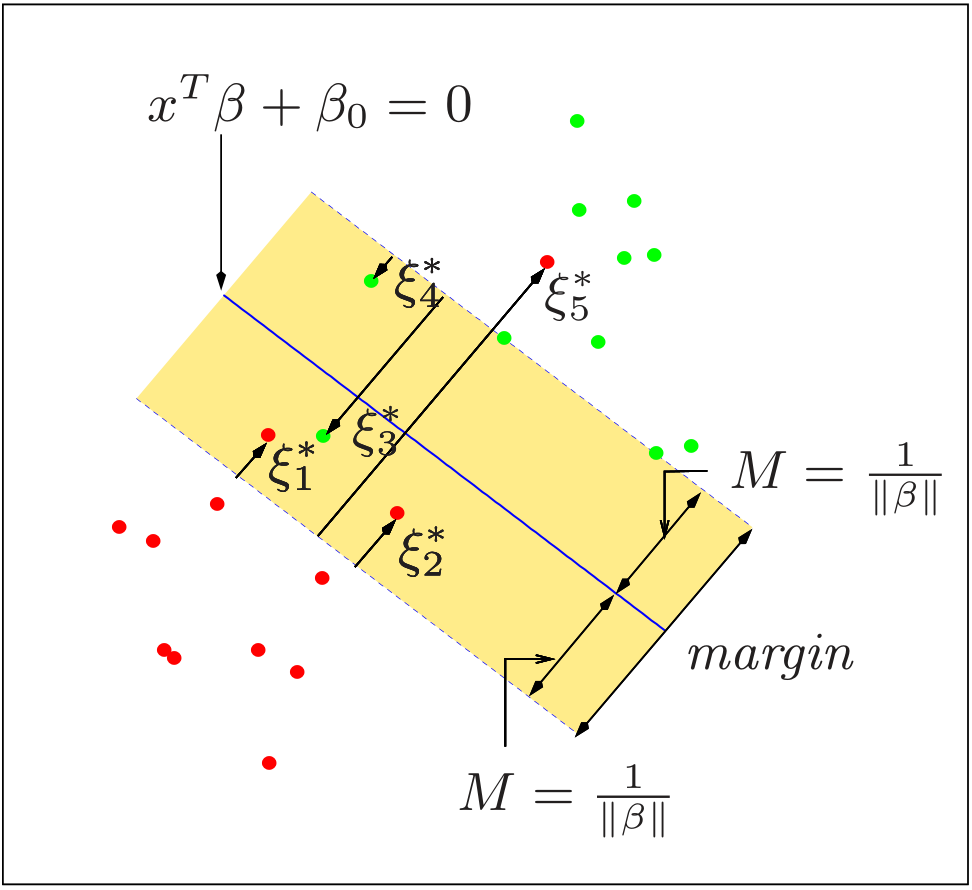
\includegraphics[width=0.4\linewidth]{pic/SVM.png}
    \caption{Support Vector Machine Illustration}
    \label{FigSVMIllustration}
\end{figure}

    Primal $ \theta _P $:
    \begin{equation*}
        \begin{aligned}
        \mathop{\arg\min}\limits_{\beta ,\beta _0:M=1/\Vert \beta  \Vert }\quad &\dfrac{1}{2}\Vert \beta  \Vert^2+C\sum_{i=1}^N\xi _i \\
        s.t.\quad & y_i(x_i'\beta +\beta _0)\geq 1-\xi _i&i=1,2,\ldots,N\\
        &\xi _i\geq 0&i=1,2,\ldots,N
        \end{aligned}
    \end{equation*}

    write the generalized lagrange function as defined in \autoref{EqaGeneralizedLagrangeFunction}:
\begin{align}
    \mathcal{L}(\beta ,\beta _0,\xi _i;\alpha ,\mu )=&\dfrac{1}{2}\Vert \beta  \Vert ^2+C\sum_{i=1}^N\xi _i+\sum_{i=1}^N\alpha _i\left[1-\xi _i-y_i(x_i'\beta +\beta _0)\right]-\sum_{i=1}^N\mu _i\xi _i \\
    s.t.\quad & \alpha _i\geq 0,\quad \mu _i\geq 0,\qquad i=1,2,\ldots,N
\end{align}
        
    dual problem is given when $ \dfrac{\partial^{} \mathcal{L}}{\partial \beta ,\beta _0,\xi _i^{}}=0 $:
\begin{align}
    \dfrac{\partial^{} \mathcal{L}}{\partial \beta ^{}}=0:\,&\hat{\beta }=\sum_{i=1}^N\alpha _iy_ix_i\\
    \dfrac{\partial^{} \mathcal{L}}{\partial \beta _0^{}}=0:\,&\sum_{i=1}^N\alpha _iy_i=0\\
    \dfrac{\partial^{} \mathcal{L}}{\partial \xi _i^{}}=0:\,&C=\alpha _i+\mu _i,\quad i=1,2,\ldots,N
\end{align}

    Dual $ \theta _D $:
\begin{align}\label{EqaDualProblemOfSVM}
    \theta _D(\alpha,\mu )=&\mathop{\min}\limits_{\beta ,\beta _0,\xi _i} \mathcal{L}=-\dfrac{1}{2}\sum_{i=1}^N\sum_{j=1}^N\alpha _i\alpha _jy_iy_jx_i'x_j+\sum_{i=1}^N\alpha _i\\
    s.t.\quad&0\leq \alpha _i\leq C\\
    &\sum_{i=1}^N\alpha _iy_i=0
\end{align}

    we can maximize $ \theta _D $ to obtain $ \hat{\alpha }_i $, $ \hat{\mu }_i=C-\hat{\alpha }_i $. And $ (\hat{\beta },\hat{\beta }_0,\xi _i) $ are given utilizing KKT condition for $ d^*=\mathop{\max}\limits_{\alpha ,\mu } \theta _D{\color{red}=}\mathop{\min}\limits_{\beta ,\beta _0,\xi _i}\theta _P=p^*  $:
\begin{align}
    &\hat{\alpha _i}\left[1-\hat{\xi }_i-y_i(x_i'\hat{\beta }+\hat{\beta }_0)\right]=0\\
    &(C-\hat{\alpha }_i)\hat{\xi }_i=0\\
    &1-\hat{\xi }_i-y_i(x_i'\hat{\beta }+\hat{\beta }_0)\leq 0\\
    &0\leq \hat{\alpha }_i\leq C\\
    &\hat{\xi }_i\geq 0\\
    &\hat{\beta }=\sum_{i=1}^N\hat{\alpha }_iy_ix_i
\end{align}

    discussion on different cases of $ \alpha _i,\xi _i $:
\begin{align}
    \hat{\alpha }_i=0:\,    &\hat{\xi }_i=0\\
    \hat{\alpha }_i=C:\,    &y_i(x_i\hat{\beta }+\hat{\beta }_0)=1-\hat{\xi }_i\\
    0<\hat{\alpha }_i<C:\,  &\hat{\xi }_0=0,\, y_i(x_i\hat{\beta }+\hat{\beta }_0)=1
\end{align}

    where all points $ \mathcal{I}^\mathrm{sv}:=  \{i^\mathrm{sv} \big|0<\hat{ \alpha }_{i^{\mathrm{sv} }}<C,\,\hat{\xi }_{i^\mathrm{sv} }=0 \} $ are called `\textbf{support vector}', that can be used to determine $ \beta _0 $:
\begin{align}
    \hat{\beta }=&\sum_{i=1}^N\hat{\alpha }_iy_ix_i=\sum_{i\in\mathcal{I}^\mathrm{sv} }\hat{\alpha }_iy_ix_i\\
    \hat{\beta }_0=&y_{i^\mathrm{sv} }-x_{i^\mathrm{sv} }'\hat{\beta }
\end{align}
    
\subsubsection{Support Vector Machine as Loss-Penalization Method}
    SVM Primal can be express in equivalent form with $ f(x_i) $ as prediction function, e.g. $ f(x_i)=\beta _0+x_i'\beta  $ for linear SVM:
    \begin{align}
        \begin{cases}
            \xi _i\geq 0\\
            \xi _i\geq 1-y_if(x_i)
        \end{cases} \Rightarrow \xi _i\geq \max\{0,1-y_if(x_i)\}= [1-y_if(x_i)]_+
    \end{align}
    
    in which $ [\,\cdot\,]_+\equiv \max\{0,\,\cdot\,\} $ is hinge loss\index{Hinge Loss}:
    \[
        \mathop{\arg\min}\limits_{\beta ,\beta _0}\sum_{i=1}^N\left[1-y_if(x_i)\right]_++\dfrac{\lambda }{2}\Vert \beta  \Vert ^2,\qquad \lambda =\dfrac{1}{C} ,\quad f(x_i)=\beta _0+x_i'\beta 
    \]
    
    which is naturally in an $ \mathop{\arg\min}\limits_{f}\sum_{i=1}^N\mathcal{L}\left(x_i,y_i,f(x_i)\right)+\dfrac{\lambda }{2}\mathcal{P}(f(\,\cdot\,))  $ Loss+Penalty form.  








\subsubsection{Kernel Support Vector Machine}




\subsection{Feature Expansion and Kernel Methods}
    Motivation: Map the data point $ x\in \mathcal{X}(e.g.\,=\mathbb{R}^p) $ to another feature space $ \mathcal{F}(e.g.\,=\mathbb{R}^M) $ (not necessarily a linear transform, usually $ M>p $, or just proper to describe the features). The mapping function lies in a Hilbert space $ \mathcal{H} $ of function:
    \[
        h(\,\cdot\,)=\left(h_1(\,\cdot\,),h_2(\,\cdot\,),\ldots,h_M(\,\cdot\,)\right)'\in \mathcal{H}:\, \mathcal{X} \to \mathcal{F}
    \]
    
    and we can construct model in feature space.    
    
\subsubsection{Reproducing Kernel Hilbert Space and The Representer Theorem}

    Based on the idea of feature space, make a step forward: the key focus of model is actually `measuring space structure by similarity between points' rather than having to define a feature space. i.e. describe similarity by a bi-linear \textbf{Kernel Function}\index{Kernel Function} 
    \[
        K(x,x') \in \mathcal{X}\times \mathcal{X}\to \mathbb{R}
    \]

    In intuition for Kernel is an `inner product kernel'. The Kernel corresponds a kind of inner product structure on $ \mathcal{H} $, the kernel should satisfies the following properties:
\begin{enumerate}[topsep=2pt,itemsep=2pt]
    \item Semi-Positive Definition:
    \begin{align}
        \int\int K(x,y)g(x)g(y)\,\mathrm{d}x\mathrm{d}y\geq 0,\quad \forall g(\,\cdot\,)
    \end{align}
    
    or an equivalent form:
    \begin{align}
        \sum_{i,j=1}^n K(x_i,x_j)a_ia_j\geq 0,\quad \forall \{x_i\}_{i=1}^m,\{a_i\}_{i=1}^n,\quad \forall n\in\mathbb{Z}^+ 
    \end{align}
    \item symmetry:
    \begin{align}
        K(x,y)=K(y,x) 
    \end{align}
\end{enumerate}



Eigenvalue $ \gamma _i $ and eigen function $ \phi _i(x) $ of Kernel:
\begin{align}
     \int_x K(x,y) \phi _i(y)\,\mathrm{d}y=\gamma _i\phi_i(x)
\end{align}

    In Hilbert space, the eigen functions are orthonormal:
    \begin{align}
         \left\langle \phi _i,\phi _j\right\rangle = \int _x\phi _i(x)\phi _j(x) \,\mathrm{d}x =\delta _{ij}
    \end{align}

    And Kernel $ K(x,y) $ could be represented from its eigen value and eigen function:
    \begin{align}
        K(x,y)=&\sum_{i}\gamma _i\phi _i(x)\phi _i(y)
        % =&\left\langle \sqrt[]{\gamma _i}\phi _i,\sqrt[]{\gamma _i}\phi _i\right\rangle 
    \end{align}

    which is Mercer's Thm.:\index{Mercer's Theorem} Semi-positive definite symmetric kernel could be expressed as an inner product form. Such a form is also called the kernel trick\index{Kernel Trick} because it usually avoid calculating inner product in high dimensional space.
    
\begin{point}
    Reproducing Kernel Hilbert Space (RKHS)\index{RKHS (Reproducing Kernel Hilbert Space)}
\end{point}

    Now use set $ \{\phi _i\} $ as the orthonormal base to form a Hilbert space $ \mathcal{H}_K=\mathrm{span}\{\phi _i\}  $ i.e. any function $ f\in\mathcal{H}_K $ could be expressed as expansion
    \begin{align}
        \mu (x)=\sum_{i} \mu _i\phi _i(x)
    \end{align}

    The inner product defined for this Hilbert space is\footnote{Hilbert space is complete linear space with inner product defined.}
    \begin{align}
        \left\langle \sum_{i}\mu _i\phi _i(x), \sum_{i}\nu _i\phi _i(x)\right\rangle _{\mathcal{H}_K} = \sum_{i}\dfrac{\mu _i\nu _i}{\gamma _i}
    \end{align}
    and norm induced by inner product
    \begin{align}
        \left\Vert f \right\Vert _{\mathcal{H}_K}=\sum_{i}\dfrac{f_i^2}{\gamma _i},\qquad f(x)=\sum_{i}f_i\phi _i(x)
    \end{align}
    
    
    
    Note: when $ x $ is fixed, $ f_x(y)= K(x,y) $ is a function of $ y $, and vice versa. Use the above expansion and inner product:
    \begin{align}
        K(x,y)=& \sum_{i}\gamma _i\phi _i(x)\phi _i(y)\\
        =&\sum_{i}\sqrt[]{\gamma _i}\phi _i(x)\sqrt[]{\gamma _i}\phi _i(y)\\
        =&\sum_{i}\dfrac{(\gamma _i\phi _i(x))(\gamma _i\phi _i(y))}{\gamma _i}\\
        =&\left\langle \sum_{i}\gamma _i\phi _i(x){\color{brown} \phi _i(\xi )},\sum_{i}\gamma _i\phi _i(y){\color{brown} \phi _i(\xi )} \right\rangle _{\mathcal{H}_K}\\
        =&\left\langle K(x,\xi ),K(\xi ,y) \right\rangle _{\mathcal{H}_K}
    \end{align}

        which is the reproducing property of Kernel $ K(\,\cdot\,,\,\cdot\,) $ and its corresponding Hilbert space $ \mathcal{H}_K $
    
\begin{point}
    Representer Thm. for RKHS
\end{point}

    With Kernel and its corresponding RKHS defined, we could write a optimization problem as loss+penalty form:
    \begin{align}\label{EqaLossPenaltyFormOfRKHS}
         \mathop{\arg\min}\limits_{f\in\mathcal{H}_K}\sum_{i=1}^N\mathcal{L}(y_i, f(x_i)) + \dfrac{\lambda }{2}\left\Vert f \right\Vert^2 _{\mathcal{H}_K}
    \end{align}

    Representer Thm.\index{Representer Theorem}: Solution to above optimization has a \textbf{finite}  form
    \begin{align}
        \hat{f}(x)=\sum_{i=1}^N\hat{\alpha }_iK(x,x_i) 
    \end{align}

    i.e. we can optimize over $ \{\hat{\alpha }_i\}_{i=1}^N $, instead of optimizing over $ \{f_i\}_{i=1}^{\infty} $.

    norm of $ \hat{f} $ is represented as 
    \begin{align}
        \left\Vert \hat{f} \right\Vert ^2 _{\mathcal{H}_K}=&\left\langle \sum_{i=1}^N\hat{\alpha }_iK(x,x_i),\sum_{i=1}^N\hat{\alpha }_iK(x,x_i) \right\rangle _{\mathcal{H}_K}\\
        =&\sum_{i=1}^N\sum_{j=1}^N\hat{\alpha }_i\hat{\alpha }_j K(x_i,x_j)
    \end{align}

    Optimization problem \autoref{EqaLossPenaltyFormOfRKHS} is parameterized by $ \{\hat{\alpha }_i\}_{i=1}^N $:
    \begin{align}\label{EqaLossPenaltyFormOfKernel}
        \mathop{\arg\min}\limits_{\{\hat{\alpha }_i\}_{i=1}^N\in \mathbb{R}^N}\sum_{i=1}^N\mathcal{L}(y_i, \sum_{j=1}^N\hat{\alpha }_jK(x_i,x_j)) + \dfrac{\lambda }{2}\sum_{i=1}^N\sum_{j=1}^N\hat{\alpha }_i\hat{\alpha }_j K(x_i,x_j)
    \end{align}

    Or written in matrix form $ y=(y_1,y_2,\ldots,y_N) $ $ \alpha =(\alpha _{1},\alpha _{2},\ldots,\alpha _{N})  $, $ K=\{K(x_i,x_j)\}_{i,j=1}^N $:
    \begin{align}
        \mathop{\arg\min}\limits_{\alpha \in \mathbb{R}^N}\sum_{i=1}^N\mathcal{L}(y, K\alpha ) + \dfrac{\lambda }{2}\alpha 'K\alpha 
    \end{align}

    Classification criterion
    \begin{align}
        \hat{f}(x) =\sum_{i=1}^N\hat{\alpha }_iK(x,x_i)
    \end{align}
    

\subsubsection{Useful Kernel}
    Some useful Kernel for numeric vector $ x $:
    \begin{itemize}[topsep=2pt,itemsep=0pt]
        \item Linear Kernel (identity):
        \begin{align}
            K(x,y):=\left\langle x,y \right\rangle 
        \end{align}        
        \item $ d^\mathrm{th}  $ Degree Polynomial Kernel\index{dth Degree Polynomial Kernel@$ d^\mathrm{th}  $ Degree Polynomial Kernel}
        \begin{align}
            K(x,y):=\left(1+\left\langle x,y \right\rangle \right)^d
        \end{align}
        \item Radical Base Function Kernel\index{RBF Kernel (Radical Base Function Kernel)}: 
        \begin{align}
            K(x,y):=\exp\left[ -\dfrac{\left\Vert x-y \right\Vert ^2}{\sigma ^2} \right] 
        \end{align}
        \item Sigmoid Kernel\index{Sigmoid Kernel}: 
        \begin{align}
            K(x,y)=\tanh\left(1+\left\langle x,y \right\rangle \right) 
        \end{align}
    \end{itemize}

    Note that \autoref{EqaLossPenaltyFormOfKernel} includes Kernel $ K(\,\cdot \,,\,\cdot \,) $ only, thus Kernel trick could be applied to various scenarios once we could define a proper Kernel. e.g. Substring Kernel for string sequence.


\subsubsection{Kernel Support Vector Machine}
    Replace the inner produce term in Dual problem of SVM \autoref{EqaDualProblemOfSVM} into Kernel function to obtain Kernel SVM:\index{KSVM (Kernel Support Vector Machine)}
    \begin{align}
         \mathop{\arg\min}\limits_{\hat{\alpha} }& \sum_{i=1}^N\hat{\alpha} _i-\dfrac{1}{2}\sum_{i=1}^N\sum_{j=1}^N\hat{\alpha} _i\hat{\alpha} _jy_iy_j K(x_i,x_j) \\
         \hat{f}(x)=\sum_{i\in\mathcal{I}^\mathrm{sv} }\hat{\alpha }_iy_iK(x,x_i)+\hat{\beta }_0
    \end{align}

    Or use the loss+penalization primmal form of SVM:
    \begin{align}
        \mathop{\arg\min}\limits_{\hat{\alpha } }&\sum_{i=1}^N\left[ 1-y_i\sum_{j=1}^N\hat{\alpha }_jK(x_i,x_j) \right]_++\dfrac{\lambda }{2}\sum_{i=1}^N\sum_{j=1}^N\hat{\alpha }_i\hat{\alpha }_jK(x_i,x_j),\quad \lambda =\dfrac{1}{C} \\
        \hat{y}(x)=&\begin{cases}
            1 &,\hat{f}(x)=\sum_{i=1}^N\hat{\alpha }_iK(x,x_i)\geq s\\
            -1&,\hat{f}(x)=\sum_{i=1}^N\hat{\alpha }_iK(x,x_i)<s
        \end{cases}
    \end{align}
    
    Note that the loss function form is $ [1-y_if(x_i)]_+ $
    
    
\subsubsection{Kernel Regression}
\begin{point}
    Kernel Regression with Squared Error Loss
\end{point}

     Recall linear regression with RS loss
     \begin{align}
        \mathop{\arg\min}\limits_{\beta_0,\beta  }\sum_{i=1}^N\left[ y_i-\beta _0-x_i'\beta  \right]^2+\dfrac{\lambda }{2}\left\Vert \beta \right\Vert^2_2
     \end{align}

     replace linear classification $ f(x)=\beta _0+x'\beta  $ into Kernel $ K\alpha  $:
     \begin{align}
        \mathop{\arg\min}\limits_{\hat{\alpha }}(y-K\hat{\alpha } )'(y-K\hat{\alpha } ) +\dfrac{\lambda }{2}\hat{\alpha } 'K\hat{\alpha } 
     \end{align}

     Solution is similar to ridge regression form:
     \begin{align}
        \hat{\alpha }=(K+\lambda I)^{-1}y 
     \end{align}     

\begin{point}
    Kernel Logistic Regression
\end{point}

    In logistic regression, the loss function is binomial deviance $ \log\left[1+e^{-yf(x)}\right] $
    \begin{align}
        \mathop{\arg\min}\limits_{\hat{\alpha } }&\sum_{i=1}^N\log \left[1+e^{y_i\sum_{j=1}^N\hat{\alpha }_jK(x_i,x_j)}\right]+\dfrac{\lambda }{2}\sum_{i=1}^N\sum_{j=1}^N  \hat{\alpha }_i\hat{\alpha }_jK(x_i,x_j)\\
        \hat{y}(x)=&\begin{cases}
            1 &,\hat{f}(x)=\sum_{i=1}^N\hat{\alpha }_iK(x,x_i)\geq s\\
            -1&,\hat{f}(x)=\sum_{i=1}^N\hat{\alpha }_iK(x,x_i)<s
        \end{cases}
    \end{align}
    

\subsection{Clustering}
    Clustering is an important scenario of unsupervised learning $ \mathcal{D}=\{x_i\}_{i=1}^N $, to cluster `similar' data points into the same group. 

\subsubsection{Proximity Matrix}
    For separation concern, we should first define some metric to measure similarity between data
    \begin{align}
        d_{ij}=D(x_i,x_j) 
    \end{align}
    common usage of distance measure see \autoref{SubSectionClusteringAnalysis}
    
    And form the proximity matrix\index{Proximity Matrix} $ W $:
    \begin{align}
    D=\{d_{ij}\}_{i,j=1}^N 
    \end{align}
    
    Usually some clustering algorithm would claim some properties:
\begin{itemize}[topsep=2pt,itemsep=0pt]
    \item Non-negative element and non-zero diagonal:
    \begin{align}
        d_{ij}\geq 0,\,\forall i,j.\qquad d_{ii}=0,\,\forall i 
    \end{align}
    \item Symmetry
    \begin{align}
        D=D^T 
    \end{align}
\end{itemize}

    Overall dissimilarity:
    \begin{align}
        \bar{D}=\dfrac{1}{N^2}\sum_{i=1}^N\sum_{j=1}^ND(x_i,x_j) 
    \end{align}

\begin{point}
    Optimizing Goal of Clustering
\end{point}

    With similarity/dissimilarity defined, clustering target could be expressed as maximizing within cluster scatter/ minimizing between cluster scatter, with respect to clustering group $ C(\, \cdot \, ) $
    \begin{align}
        \mathop{\arg\max}\limits_{C(\, \cdot \, )}\dfrac{1}{2}\sum_{k=1}^K\sum_{i:C(x_i)=k}\sum_{j:C(x_j)=k}D(x_i,x_j)\\
        \mathop{\arg\min}\limits_{C(\, \cdot \, )}\dfrac{1}{2}\sum_{k=1}^K\sum_{i:C(x_i)=k}\sum_{j:C(x_j)\neq k}D(x_i,x_j)
    \end{align}

    The two forms are equivalent due to a fixed sum:
    \begin{align}
        \dfrac{1}{2}\sum_{k=1}^K\sum_{i:C(x_i)=k}\sum_{j:C(x_j)=k}D(x_i,x_j)+\dfrac{1}{2}\sum_{k=1}^K\sum_{i:C(x_i)=k}\sum_{j:C(x_j)\neq k}D(x_i,x_j)=\dfrac{1}{2}\sum_{i=1}^N\sum_{j=1}^ND(x_i,x_j):=T=\mathrm{const}
    \end{align}

    Usually search for cluster assignment is based on iterative greedy descent search.
    
    Some frequently used clustering methods are included in \autoref{SubSectionClusteringAnalysis}
    \begin{itemize}[topsep=2pt,itemsep=0pt]
        \item Hierarchical Method
        \item $ K $-Means
        \item EM-Gaussian Mixture Model
        \item DBSCAN \& OPTICS Density Method
    \end{itemize}
    
    In this section, an extra model based on spectrum is introduced

\subsubsection{Spectrum Clustering}
    Express the dataset as a Graph $ \mathcal{G}=(\mathcal{V},\mathcal{E},\mathcal{W}) $, where $ \mathcal{V}=\{v_i\}_{i=1}^N $ for vertex, $ \mathcal{E}=\{e_{ij}\}_{i,j=1}^N $, $ \mathcal{W}=\{w_{ij}\}_{i,j=1}^N $ for edges and weights. In this case cluster is a graph partition problem.

\begin{point}
    Graph Laplacian \index{Graph Laplacian}
\end{point}

Some definition:

\begin{itemize}[topsep=2pt,itemsep=0pt]
    \item Degree of vertex:
    \begin{align}
        d_i=\sum_{j=1}^Nw_{ij} 
    \end{align}
    \item Degree matrix
    \begin{align}
        D=\mathrm{diag}\{d_1,d_2,\ldots ,d_N\} 
    \end{align}
    \item Unnormalized graph Laplacian:
    \begin{align}
        L:= D-W
    \end{align}

    is symmetric and semi-positive definite
    \begin{align}
        \xi 'L\xi =\sum_{i,j=1}^Nw_{ij}(\xi _i-\xi _j)^2\geq 0,\quad\forall \xi \in\mathbb{R}^N 
    \end{align}
    
\end{itemize}

    Spectrum is based on studying the eigen vector and eigen value of $ L $.
\begin{itemize}[topsep=2pt,itemsep=0pt]
    \item For any graph Laplacian $ \mathop{L}\limits_{m\times m}  $, $ \mathbf{1}_m $ is a eigen vector with eigen value $ 0 $
    \item In the case that $ \mathcal{G} $ is \textbf{not} fully connected, with $ K $ subgraph $ \mathcal{G}=\{\mathcal{G}_1,\mathcal{G}_2,\ldots,\mathcal{G}_K\} $, i.e. $ W $ and $ L $ could be written in diagonal form (usually need some row/column transformation)
    \begin{align}
        L=\begin{bmatrix}
        L_{1}&0&\ldots&0\\
        0&L_{2}&\ldots&0\\
        \vdots&\vdots&\ddots&\vdots\\
        0&0&\ldots&L_{K}\\
        \end{bmatrix} 
    \end{align}

    the multiplicity of eigen value $ 0 $ is $ K $, with each eigen vector as
    \begin{align}
         \mathbf{1}_{\mathcal{G}_k}=[\mathbb{I}(v_1\in \mathcal{G}_k),\ldots,\mathbb{I}(v_N)\in\mathcal{G}_k],\quad k=1,2,\ldots,K
    \end{align}
    \item In real world case, the graph could probably expressed as a small deviance from a graph with subgraph:
    \begin{align}
         L=\begin{bmatrix}
            L_{1}&0&\ldots&0\\
            0&L_{2}&\ldots&0\\
            \vdots&\vdots&\ddots&\vdots\\
            0&0&\ldots&L_{K}\\
            \end{bmatrix} +\mathop{N\times N}\limits_{\delta } 
    \end{align}
    
    where we would expect the smallest $ K $ eigen value $ 0=\lambda _1\leq \lambda _2\leq\ldots \leq \lambda _K $ corresponds to the $ K $ cluster we want.

     
\end{itemize}

\begin{algorithm}{Spectral Clustering}
    \begin{enumerate}[topsep=2pt,itemsep=2pt]
        \item Compute $ \mathop{L}\limits_{N\times N}  $
        \item Determine the $ K $ smallest eigen values $ 0=\lambda _1\leq \lambda _2\leq\ldots \leq \lambda _K $ with eigen vector $ u_i $, $ i=1,2,\ldots,K $
        \begin{align}
            U=&[u_1,u_2,\ldots,u_K]=\begin{bmatrix}
            u_{11}&u_{12}&\ldots&u_{1K}\\
            u_{21}&u_{22}&\ldots&u_{2K}\\
            \vdots&\vdots&\ddots&\vdots\\
            u_{N1}&u_{N2}&\ldots&u_{NK}\\
            \end{bmatrix} 
            =[z_1,z_2,\ldots,z_N]^T\\
            z_i=&[u_{i1},u_{i2},\ldots,u_{iK}]^T,\quad i=1,2,\ldots,N
        \end{align}
    
        \item Cluster $ \{z_i\}_{i=1}^N$ with e.g. $ K $-Means.
    \end{enumerate}
    
        
\end{algorithm}


    Choice of normalized graph Laplacian, would cause different cluster results:
\begin{itemize}[topsep=2pt,itemsep=0pt]
    \item Ratio Cut $ L=I-D^{-1}W $
    \begin{align}
        \mathop{\arg\min}\limits_{\{\mathcal{G}_1,\ldots,\mathcal{G}_K\}}\dfrac{1}{2}\sum_{i=1}^K\dfrac{\mathrm{Bet}(\mathcal{G}_i,\mathcal{G}_{i}^\complement)}{|\mathcal{G}_i|}  
    \end{align}
    \item Normalized Cut $ L=I-D^{-1/2}WD^{-1/2} $
    \begin{align}
        \mathop{\arg\min}\limits_{\{\mathcal{G}_1,\ldots,\mathcal{G}_K\}}\dfrac{1}{2}\sum_{i=1}^K\dfrac{\mathrm{Bet}(\mathcal{G}_i,\mathcal{G}_{i}^\complement)}{\sum_{i\in\mathcal{G}_i}\sum_{j\in\mathcal{G}}d_{ij}}  
    \end{align}
    
\end{itemize}

\subsection{Tree-Based Classification Model}
    Idea of tree: divide the space $ \mathcal{X} $ into grids $ R_m $ and assign prediction into the most frequent class
    \begin{align}
        \hat{f}(x\in R_m)=\mathop{\arg\max}\limits_{k} \sum_{x_i\in R_m}\mathbb{I}(y_i=k)
    \end{align}

    But such method is not practical in high dimensional due to curse of dimensionality. Nore practical method would be a greedy search, each step along one variable.

\subsubsection{Tree-Based Classification}

\begin{point}
    Branch Growing Process
\end{point}

    Grow branch on a node $  $

\begin{algorithm}{Classification Tree}
    In each branck growing on a node:
    \begin{enumerate}[topsep=2pt,itemsep=2pt]
        \item Look for a splitting variable $ x_j $ and split value $ s $:
        \begin{align}
            &\mathop{\arg\min}\limits_{j,s}\left[N_\mathrm{left} \mathrm{ImPu}(x_i\in R_\mathrm{left}(j,s) )+N_\mathrm{right} \mathrm{ImPu}(x_i\in R_\mathrm{right}(j,s) )  \right] \\
            &R_\mathrm{left}(j,s)=\{x:x_j\leq s\},\quad R_\mathrm{right}(j,x)=\{x:x_j>s\}   
        \end{align}
        
        useful impurity measure $ \mathrm{ImPu}(\{x\})  $ with $ p_k(X=\{x\})$ defined
        \begin{align}
            p_k(X)=\dfrac{\sum_{x\in X}\mathbb{I}(C(x)=k)}{|X|}
        \end{align}
        
        
        \begin{itemize}[topsep=2pt,itemsep=0pt]
            \item Misclassification rate
            \begin{align}
                1-\mathop{\max}\limits_{k} p_k 
            \end{align}
            \item Gini impurity\index{Gini Impurity}
            \begin{align}
                \sum_{k=1}^Kp_k(1-p_k)=\sum_{k=1}^K\sum_{k'\neq k}p_kp_{k'} 
            \end{align}
            
            Gini impurity with category weight $ \mathop{W_K}\limits_{K\times K}=\{w_{kk'}\}_{k,k'=1}^K  $
            \begin{align}
                \sum_{k=1}^K\sum_{k'\neq k}w_{kk'}p_kp_{k'} 
            \end{align}
            
            \item Entropy
            \begin{align}
                -\sum_{k=1}^Kp_k\log p_k 
            \end{align}
            
            
            
            
        \end{itemize}
        \item usually the process ends when 
        \begin{align}
            |\mathrm{node} |\leq \mathrm{const},\quad \forall \mathrm{node}  
        \end{align}
        
        \item Apply cost complexity pruning strategy
        \begin{align}
            C_\alpha (T) =\sum_{m=1}^{|T|}N_m\mathrm{ImPu}(R_m)+\alpha |T|
        \end{align}
        
        where $ T $ is tree, $ |T| $ for number of nodes in the tree.
        
    \end{enumerate}
    
        
    
\end{algorithm}
    

    Comment:
\begin{itemize}[topsep=2pt,itemsep=0pt]
    \item Tree methods is well-interpreted, especially similar to a natural desicion making process
    \item Handle non-linear classification pattern
    \item Unstable to data.
\end{itemize}

    Performance of tree classification could be largely improved with bagging method and boosting method.

    

\subsubsection{Bagging and Boosting}
    
\begin{point}
    Bagging\index{Bagging Method (Bootstrap Aggregation Method)}\index{Bootstrap Aggregation}
\end{point}

    Bagging is short for \textbf{B}ootstrap \textbf{Ag}gregation. Idea: for $ B $ boostrapped training data, the boostrapping result
    \begin{align}
        \hat{f}_\mathrm{boot}(x)=\dfrac{1}{B}\sum_{b=1}^B\hat{f}_b(x)  \text{ or }=\mathop{\arg\max}\limits_{k} \sum_{b=1}^B\mathbb{I}(\hat{f}_b(x)=k)
    \end{align}

\begin{point}
    Random Forest\index{Random Forest}
\end{point}

    Random Forest aims at decorrelating trees to reduce variance when averaging trees.

\begin{algorithm}{Random Forest Bagging}
    \begin{enumerate}[topsep=2pt,itemsep=2pt]
        \item Generate $ B $ different boostrapped training data. (\textit{random 1} by bootstrap sampling)
        \item For each sample, grow a tree. In each split of tree (i.e. a branch growth), $ q\approx \sqrt[]{p} $ variable components are randomly selected for classification. (\textit{random 2} by randomizing components)
        \item Take average or vote of all $ B $ trees as the final result
    \end{enumerate}
    
    Comment: A prune is usually needed, cause variance is reduced by averaging.
        
\end{algorithm}
    
\begin{point}
    Boosting\index{Boosting Method}
\end{point}

    Idea: Fitting result of previous trees could be used to modify following trees. The error rate of each tree would influence the vote weight when bagging the results.
\index{Adaboost}

\begin{algorithm}{Adaboost}
    \begin{enumerate}[topsep=2pt,itemsep=2pt]
        \item Each observant is given weights $ w_i^{(0)}=\dfrac{1}{N},\,i=1,2,\ldots,N $
        \item For $ m=1:M $, $ M $ for loops of boosting:
        \begin{enumerate}[topsep=2pt,itemsep=2pt]
            \item Grow a tree $ T^{(m)}(x) $ with weight $ w_i^{(m)} $
            \item Compute \textbf{error rate}
            \begin{align}
                \mathrm{err}^{(t)} :=\dfrac{\sum_{i=1}^Nw_i^{(m)}\mathbb{I}(y_i\neq T^{(m)}(x_i))}{\sum_{i=1}^Nw_i^{(m)}}
            \end{align}

            and define 
            \begin{align}
                 \alpha ^{(m)}=\log\left[(1-\mathrm{err}^{(m)} )\big/\mathrm{err}^{(m)}\right]
            \end{align}
            \item Reset weights by
            \begin{align}
                w_i ^{(m+1)}=w^{(m)}\cdot\exp\left[ \alpha ^{(m)}\mathbb{I}(y_i\neq T^{(m)}(x_i)) \right]
            \end{align}
         
        \end{enumerate}
        \item Output
        \begin{align}
            \hat{f}(x)=\mathrm{sgn}\left[\sum_{m=1}^M\alpha ^{(m)}T^{(m)}(x)\right]  
        \end{align}
        
        
            
    \end{enumerate}
    
        
\end{algorithm}
    

\subsection{Neural Network}
\index{Neural Network}
\begin{point}
    Linear Perceptron with Activate Function\index{Linear Perceptron}\index{Activate Function}
\end{point}

    Usually linear perceptron is used as a neuron in neutral network:
    \begin{align}
        y=g(w_0+w_1x_1+\ldots+w_px_p) =g(x'w),\quad x_0\equiv 1
    \end{align}

    where $ g(\, \cdot \, ) $ is activate function. Such Perceptron could be optimized by gradient

    Some useful activate function:
\begin{itemize}[topsep=2pt,itemsep=0pt]
    \item Linear Threshold Unit (LTU)\index{LTU (Linear Threshold Unit)}\index{Activate Function!LTU (Linear Threshold Unit)}
    \begin{align}
        g(\xi )=\begin{cases}
            0,& \xi < 0\\
            1,& \xi \geq 0
        \end{cases} =\eta(\xi )
    \end{align}
    \item Logistic Function\index{Activate Function!Logistic Function}
    \begin{align}
        g(\xi )=\dfrac{1}{1+e^{-\xi } } 
    \end{align}
    \item Hyperbolic Tangent Function\index{Activate Function!Hyperbolic Tangent Function}
    \begin{align}
        g(\xi )=\tanh \xi =\dfrac{e^{2\xi }-1}{e^{2\xi }+1} 
    \end{align}
    \item Rectified Linear Unit (ReLU)\index{ReLU (Rectified Linear Unit)}\index{Activate Function!ReLU (Rectified Linear Unit)}
    \begin{align}
        g(\xi )= \begin{cases}
            0,& \xi < 0\\
            \xi ,& \xi \geq 0
        \end{cases}
    \end{align}
\end{itemize}

\begin{figure}[H]
    \centering
\def\layersep{2.5cm}
\begin{tikzpicture}[shorten >=1pt,->,draw=black!50, node distance=\layersep]
    \tikzstyle{every pin edge}=[<-,shorten <=1pt]
    \tikzstyle{neuron}=[circle,minimum size=12pt,draw=black,inner sep=0pt]
    \tikzstyle{input neuron}=[neuron];
    \tikzstyle{output neuron}=[neuron];
    \tikzstyle{hidden neuron}=[neuron];
    \tikzstyle{annot} = [align=left]

    % % Draw the input layer nodes
    % \foreach \name / \y in {1,...,4}
    % % This is the same as writing \foreach \name / \y in {1/1,2/2,3/3,4/4}
    %     \node[input neuron, pin=left:Input \#\y] (I-\name) at (0,-\y) {};

    \foreach \name / \x in {1,...,4}
        \node[neuron] (I-\name) at (-\x cm,-\layersep) {};
    \foreach \name / \x in {1,...,6}
        \path[xshift=1cm]
        node[neuron] (H-\name) at (-\x cm,0) {};
    \foreach \name / \x in {1,...,3}
        \path[xshift=-0.5cm]
        node[neuron] (O-\name) at (-\x cm,\layersep) {};
    \node[annot] (Error) at (-2.5 cm,2*\layersep) {$ \mathcal{L}=\dfrac{1}{2}\sum_{j=1}^l\left( \hat{y}_j-y_j \right)^2 $};
    \foreach \bg in {1,...,4}
        \foreach \ed in {1,...,6}
            \path (I-\bg) edge (H-\ed);
    \foreach \bg in {1,...,6}
        \foreach \ed in {1,...,3}
            \path (H-\bg) edge (O-\ed);
    \foreach \bg in {1,...,3}
        \path (O-\bg) edge (Error);
    
    \node[annot] at (I-1) {\small$ x_d $};
    \node[annot] at (H-1) {\small$ b_q $};
    \node[annot] at (O-1) {\small$ y_l $};


    \node[annot,right of=H-1, node distance=3.58cm] (hr) {$ \hat{b}_h=f(\sum_{i=1}^dv_{ih}x_i-\gamma  _h) ,\, h=1,\ldots,q$};
    \node[annot,right of=O-1, node distance=5.1cm] (or) {$ \hat{y}_j=f(\sum_{h=1}^qw_{hj}\hat{b}_h-\theta _j) ,\,j=1,\ldots,l $};
    \node[annot,right of=I-1, node distance=2.7cm] (ir) {$ x_i,\,i=1,\ldots,d $};
    \node[annot,left of=I-4, node distance=3cm] (il) {Input Layer};
    \node[annot,left of=H-6, node distance=2cm] (hl) {Hidden Layer};
    \node[annot,left of=O-3, node distance=3.5cm] (ol) {Output Layer};

    % % Draw the hidden layer nodes
    % \foreach \name / \y in {1,...,5}
    %     \path[yshift=0.5cm]
    %         node[hidden neuron] (H-\name) at (\layersep,-\y cm) {};

    % % Draw the output layer node
    % \node[output neuron,pin={[pin edge={->}]right:Output}, right of=H-3] (O) {};

    % % Connect every node in the input layer with every node in the
    % % hidden layer.
    % \foreach \source in {1,...,4}
    %     \foreach \dest in {1,...,5}
    %         \path (I-\source) edge (H-\dest);

    % % Connect every node in the hidden layer with the output layer
    % \foreach \source in {1,...,5}
    %     \path (H-\source) edge (O);

    % % Annotate the layers
    % \node[annot,above of=H-1, node distance=1cm] (hl) {Hidden layer};
    % \node[annot,left of=hl] {Input layer};
    % \node[annot,right of=hl] {Output layer};
\end{tikzpicture}

\caption{Structure of Feed-Forward Neural Network (1 Layer)}
\label{FigureMLP}
\end{figure}
    
    
    A MonoLayer perceptron with enough neurons (hidden units) could represent any coutinuous function. MultiLayer Perceptron (MLP)\index{MLP (MultiLayer Perceptron)} could even represent discontinuous functions. 
    
\subsubsection{Back Propagation}
    Perceptron system is usually optimized by back propagation (of gradient)\index{BP (Back Propagation)}.

    An example to optimize $ v_{ih},\,\gamma _h $ in \autoref{FigureMLP}:
    \begin{align}
        \dfrac{\partial^{} \mathcal{L}}{\partial v_{ih}}=&\sum_{j=1}^l\dfrac{\partial^{} \mathcal{L}}{\partial \hat{y}_j^{}}\dfrac{\partial^{} \hat{y}_j}{\partial \hat{b}_h^{}}\dfrac{\partial^{} \hat{b}_h}{\partial v_{ih}}\\
        =&\sum_{j=1}^l\hat{y}_j(\hat{y}_j-y_j)\cdot \dfrac{\partial^{} f(u)}{\partial u^{}}\Big|_{u=\sum w_{hj}\hat{b}_h-\theta _j}w_{hj}\cdot \dfrac{\partial^{} f(v)}{\partial v^{}}\Big|_{v=\sum_{i=1}^dv_{ih}x_i-\gamma _h}x_i\\
        \dfrac{\partial^{} \mathcal{L}}{\partial \gamma _h}=&\sum_{j=1}^l\dfrac{\partial^{} \mathcal{L}}{\partial \hat{y}_j^{}}\dfrac{\partial^{} \hat{y}_j}{\partial \hat{b}_h^{}}\dfrac{\partial^{} \hat{b}_h}{\partial \gamma _h}\\
        =&\sum_{j=1}^l\hat{y}_j(\hat{y}_j-y_j)\cdot \dfrac{\partial^{} f(u)}{\partial u^{}}\Big|_{u=\sum w_{hj}\hat{b}_h-\theta _j}w_{hj}\cdot \dfrac{\partial^{} f(v)}{\partial v^{}}\Big|_{v=\sum_{i=1}^dv_{ih}x_i-\gamma _h}\cdot (-1)
    \end{align}
    
    


\newpage

\section{应用时间序列部分}
\begin{center}
    Instructor: Dong Li
\end{center}

% Time series modelling usually concerns \textbf{forecasting}, i.e. predict future behaviour of a quantity based on history information. A direct method is modelling a time series object, with history and future are included in it. In this section several modelling/forecasting methods would be included.

\subsection{Time Series Data and Model}


\subsubsection{Time Series Data and Tasks}
    \textbf{Time Series} : a sequential r.v. indexed in time order.\index{Time Series}
    \begin{equation}
        \{Y_t\},\,t\in \mathcal{T}\quad \mathcal{T}\text{ is index set} 
    \end{equation}

    and actual data of time series, i.e. times series data is called a \textbf{Realization}  of time series, denoted\footnote{A note on $ T\subset \mathcal{T} $: actually $ T $ has to be discrete beacuse it is a sample of $ \mathcal{T} $. while $ \mathcal{T} $ is not necessarily defined as discrete.}
    \[
        \{y_t\},\,t\in  T\subset\mathcal{T}
    \]
    e.g. in forecasting task, $ T $ encodes history. In this chapter we usually focus on easier case of arithmetic progression $ T=\{1,2,\dots,N\} $, or at least numeric orderal sequence.

    Time Series Analysis (TSA)\index{TSA (Time Series Analysis)}: Analysis on time series data to extract meaningful statistics/other characteristics. Task of TSA includes:
    \begin{itemize}[topsep=2pt,itemsep=0pt]
        \item Describing and Explanaing the machanism of time series 
        \item Forecasting
        \item Guiding the intervention of Time Series
    \end{itemize}

    In this section several modelling/forecasting methods would be included.
    
    % Classification:
    % \begin{itemize}[topsep=2pt,itemsep=0pt]
    %     \item Standard: dimensionality:
    %     \begin{itemize}[topsep=2pt,itemsep=0pt]
    %         \item univariate
    %         \item multivariate
    %         \item high-dimensional: e.g. tensor
    %     \end{itemize}
    %     \item Standard: Regularity of sampling time
    %     \begin{itemize}[topsep=2pt,itemsep=0pt]
    %         \item regular TS
    %         \item irregular TS
    %     \end{itemize}
    %     \item Standard: Discrete/Continuous, including data discrete/continuous or time discrete/continuous. Most common: discrete time$ + $continuous data      
    % \end{itemize}

\subsubsection{Time Series Model}
    There are plenty of useful modelling methods:
    \begin{itemize}[topsep=2pt,itemsep=0pt]
        \item Regression Model: View $ y $ as function of $ t $, regression on some model $ y=f(t) $ with loss $ \mathcal{L} $. e.g. linear regression
        \begin{align}
            y=\beta _0+\beta _1t+\varepsilon ,\quad \mathcal{L}=\sum_{t\in T}(y_t-\hat{y}_t)^2 
        \end{align}
        
        Modelling strategy is similar to that introduced in linear regression, see \autoref{SecLinearRegressionAnalysis} 
        
        \item STL Method: Seasonal and Trend decomposition using Loess. A decomposition of time series into `TS = Trend + Season + Random', i.e.\index{STL Model (Seasonal and Trend Decomposition using Loess)}
        \begin{equation}
            Y_\tau=T_\tau+S_\tau+X_\tau 
        \end{equation}
    
        and we could model $ T_\tau $, $ S_{\tau} $, $ X_\tau $ separately. The focus is the modelling of random term $ X_t $, which we expect to be `stationarily random' through time. (Usually we model this part also by ARMA model)

        \item Exponential Smoothing Model: Use weighted average over history to predict future.

        \item ARIMA Model: The main focus of this chapter.
    \end{itemize}
    

    % where randomness lies in the (usually a zero mean stationary sequence) random term $ X_\tau $. After modelling non-random $ T_\tau  $, $ S_\tau  $, our target is to estimate the zero-mean stationary $ R_\tau \equiv X_\tau  $ based on history till $ t $ ($ \tau>t $).





\subsection{Stochastic Process and Statistics}\label{SubSectionStochasticProcessForTimeSeries}
\subsubsection{Basic Knowledge of Stochastic Process}
    A stochastic process can be denoted:\index{Stochastic Process}
    \begin{equation}
        \{X_t:\,t\in \mathcal{T}\}:\, \Omega\times \mathcal{T}\to \mathcal{E}
    \end{equation}
    
\begin{point}
    Some important cases of stochastic process:
\end{point}

    
    \begin{itemize}[topsep=2pt,itemsep=0pt]
        \item i.i.d. sequence: $ \varepsilon _t\,\mathrm{i.i.d.}\sim \varepsilon   $        
        \item White Noise\index{WN (White Noise)}: uncorrelated for different subscript $ t $ in the sense of $ 2^\mathrm{nd}  $ moment, $ \varepsilon _t\sim \mathrm{WN}(\mu ,\sigma ^2)  $. where
        \begin{align}
            \mathbb{E}\left( \varepsilon _t \right) =&\mu \\
            cov(\varepsilon _t,\varepsilon _s)=&\sigma ^2\delta _{t,s}
        \end{align}

        Further we can append more constraints on $ \mathrm{WN}  $:
        \begin{itemize}[topsep=2pt,itemsep=0pt]
            \item[+] $ \{\varepsilon _t\} $ independent: independent white noise $ \varepsilon _t\sim \mathrm{IWN}(\mu ,\sigma ^2)  $ 
            \item[+] $ \mu =0 $: zero-mean white noise $ \varepsilon _t\sim \mathrm{WN}(0 ,\sigma ^2)  $
            \item[+] $ \mu =0 $, $ \sigma ^2=1 $: standard white noise $ \varepsilon _t\sim \mathrm{WN}(0,1)  $
            \item[+] $ \varepsilon \sim N(\mu ,\sigma ^2) $: normal white noise.
        \end{itemize}
        \item Martingale difference sequence (MDS)\index{MDS (Martingale Difference Sequence)}: zero expectation given history information: $ \varepsilon _t\sim \mathrm{MDS}  $, where
        \begin{align}
            \mathbb{E}\left( |\varepsilon _t| \right) <&\infty\\
            \mathbb{E}\left( \varepsilon _t|\mathcal{F}_{t-1} \right) =&0
        \end{align}

        where $ \mathcal{F}_\tau $ denotes the history until time $ \tau $:
        \begin{equation}
            \mathcal{F}_\tau\equiv \sigma \left(\varepsilon _s,\, s\leq \tau\right)\{\varepsilon _s,\varepsilon _{s-1},\varepsilon _{s-2},\ldots\} 
        \end{equation}
    \end{itemize}

    Relation: i.i.d. $ > $ MDS $ > $ WN $ > $ Stationary
    

{
\begin{figure}[H]
    \centering
    \tikzset{every picture/.style={line width=0.75pt}} %set default line width to 0.75pt        

    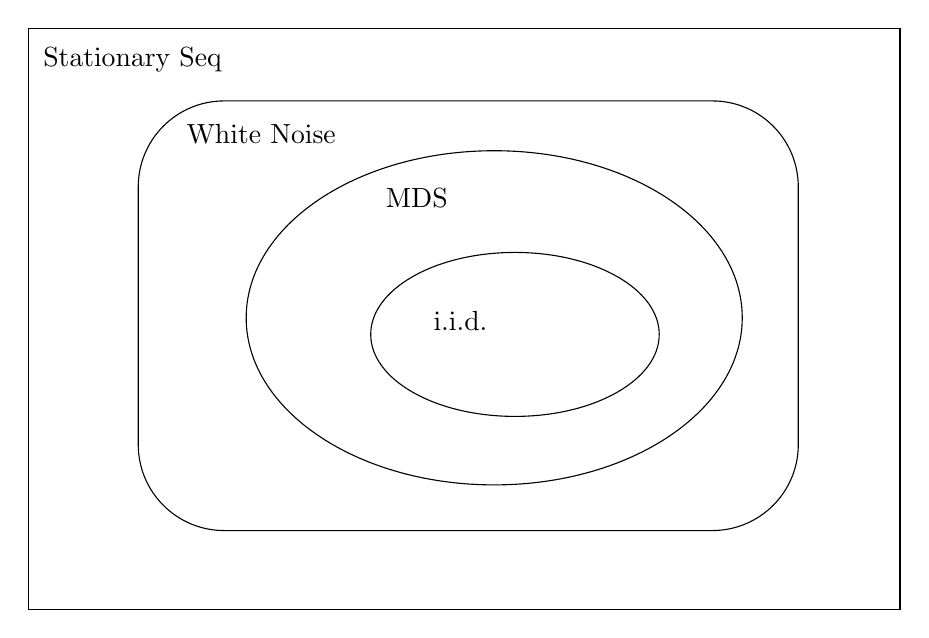
\begin{tikzpicture}[x=0.75pt,y=0.75pt,yscale=-1,xscale=1]
    %uncomment if require: \path (0,300); %set diagram left start at 0, and has height of 300
    
    %Shape: Rectangle [id:dp7367101782277172] 
    \draw   (115,13) -- (535.01,13) -- (535.01,293.02) -- (115,293.02) -- cycle ;
    %Rounded Rect [id:dp15861413740766106] 
    \draw   (168.01,89.42) .. controls (168.01,66.55) and (186.54,48.02) .. (209.41,48.02) -- (444.61,48.02) .. controls (467.47,48.02) and (486.01,66.55) .. (486.01,89.42) -- (486.01,213.62) .. controls (486.01,236.48) and (467.47,255.02) .. (444.61,255.02) -- (209.41,255.02) .. controls (186.54,255.02) and (168.01,236.48) .. (168.01,213.62) -- cycle ;
    %Flowchart: Connector [id:dp04508204736671462] 
    \draw   (220.01,152.52) .. controls (220.01,108.06) and (273.51,72.02) .. (339.51,72.02) .. controls (405.51,72.02) and (459.01,108.06) .. (459.01,152.52) .. controls (459.01,196.98) and (405.51,233.02) .. (339.51,233.02) .. controls (273.51,233.02) and (220.01,196.98) .. (220.01,152.52) -- cycle ;
    %Flowchart: Connector [id:dp3377595494528831] 
    \draw   (280.01,160.52) .. controls (280.01,138.7) and (311.13,121.02) .. (349.51,121.02) .. controls (387.89,121.02) and (419.01,138.7) .. (419.01,160.52) .. controls (419.01,182.33) and (387.89,200.02) .. (349.51,200.02) .. controls (311.13,200.02) and (280.01,182.33) .. (280.01,160.52) -- cycle ;
    
    
    % Text Node
    \draw (309,148) node [anchor=north west][inner sep=0.75pt]   [align=left] {i.i.d.};
    % Text Node
    \draw (286,89) node [anchor=north west][inner sep=0.75pt]   [align=left] {MDS};
    % Text Node
    \draw (190,58) node [anchor=north west][inner sep=0.75pt]   [align=left] {White Noise};
    % Text Node
    \draw (121,21) node [anchor=north west][inner sep=0.75pt]   [align=left] {Stationary Seq};
    
    
    \end{tikzpicture}
    \caption{Relation bet. Sequences}
\end{figure}
}


\begin{point}
    Measure of dependence within stochastic process
\end{point}

    Given a stochastic process $ \{X_t:\,t\in \mathcal{T}\} $

    \begin{itemize}[topsep=2pt,itemsep=0pt]
        \item Mean Function
        \begin{align}
            \text{Mean: }\mu _t\equiv &\mathbb{E}\left( X_t \right),&\mathcal{T}\mapsto  &\mathbb{R}
        \end{align}        
        
        \item AutoCovariance Function (ACVF) and AutoCorrelation Function (ACF):\index{ACVF (Autocovariance)}\index{ACF (Autocorrelation)}
        \begin{align}
            \text{ACVF: }\gamma _{t,s}\equiv &cov(X_t,X_s),& \mathcal{T}\times \mathcal{T}\mapsto&\mathbb{R}\\
            \text{ACF: }\rho  _{t,s}\equiv &corr(X_t,X_s)=\dfrac{\gamma _{t,s}}{\sqrt[]{\gamma _{t,t}\gamma _{s,s}}},& \mathcal{T}\times \mathcal{T}\mapsto& [-1,1]
        \end{align}

        \item Stationarity: Stationarity is a measure that the `correlation structure of stochastic process looks the same' at any time $ t $, i.e. is stationary through time.
        \begin{itemize}[topsep=2pt,itemsep=0pt]
            \item Weakly Stationary (WS)\index{WS (Weakly Stationary)}: given $ \mathbb{E}\left( X_t^2 \right) < \infty $, has const $ \mathbb{E}\left[  \right]  $ and $ cov  $ (independent of time)
            \begin{align}
                \mathbb{E}\left( X_t \right) =&\mu _t=\mu \\
                cov(X_t,X_t+k)=&\gamma _{t,t+k}=\gamma _k\independent t
            \end{align}

            \item Strictly Stationary (SS)\index{SS (Strictly Stationary)}: joint distribution invariant through time. For any given $ \{t_1,t_2,\ldots,t_n\}\subset \mathcal{T} $
            \begin{equation}
                f_{X_{t_1},X_{t_2},\ldots,X_{t_n}}=f_{X_{t_1+h},X_{t_2+h},\ldots,X_{t_n+h}},\quad \forall h 
            \end{equation}
            
        \end{itemize}

        Some note on WS and SS:
        \begin{itemize}[topsep=2pt,itemsep=0pt]
            \item Generally speaking, WS and SS are not equivalant, WS $ \nLeftrightarrow $ SS (note that SS does not put constraint on $ \mathbb{E}\left( X_t^2 \right)  $)
            \item equivalent for gaussian stochastic process.
            \item ACF and ACVF of WS: 
            \begin{align}
                \gamma _{t,t+k}=&\gamma _k=\gamma _{-k},\quad \forall t\in\mathcal{T}\\
                \rho _{t,t+k}=&\rho _k=\dfrac{\gamma _k}{\gamma _0},\quad\, \forall t\in\mathcal{T}
            \end{align}

            Notation of ACVF matrix:
            \begin{equation}
                \Gamma _k=\{\gamma _{i-j}\}_{i,j=1}^k=\begin{bmatrix}
                    \gamma _0&\gamma _1&\gamma _2&\cdots&\gamma _{k-2}&\gamma _{k-1}\\
                    \gamma _1&\gamma _0&\gamma _1&\cdots&\gamma _{k-3}&\gamma _{k-2}\\
                    \gamma _2&\gamma _1&\gamma _0&\cdots&\gamma _{k-4}&\gamma _{k-3}\\
                    \vdots&\vdots&\vdots&\ddots&\vdots&\vdots\\
                    \gamma _{k-2}&\gamma _{k-3}&\gamma _{k-4}&\cdots&\gamma _0&\gamma _1\\
                    \gamma _{k-1}&\gamma _{k-2}&\gamma _{k-3}&\cdots&\gamma _1&\gamma _0
                \end{bmatrix}_{k\times k}
            \end{equation}

            $ \Gamma _k $ is semi-positive definite. 
            \begin{equation}
                \sum_{i=1}^k\sum_{j=1}^k\alpha _i\alpha_ j\gamma _{|t_i-t_j|}\geq 0,\quad \forall k,\{t_1,\ldots,t_k\} ,\vec{\alpha }
            \end{equation}
            
        \end{itemize}
        \item Partial Autocorrelation (PACF)\index{PACF (Partial Autocorrelation)}: correlation given information between two time points, orginal definition
        \begin{align}\label{EqaPartialAutoCorrelation}
            \phi _{11}=&\phi _1\\
            \phi _{kk}=&corr\big(X_t-L(X_t|X_{t+1},\ldots,X_{t+k-1}),X_{t+k}-L(X_{t+k}|X_{t+1},\ldots,X_{t+k-1})\big),\quad k\geq 2
        \end{align}

        where $ L(X_{\tau}|X_{t+1},\ldots,X_{t+k-1}) $ is the \textbf{Best Linear Estimation}  of linear model 
        \begin{align}
             X_\tau = \beta _0+\beta _1X_{t+1}+\ldots+\beta _{k-1}X_{t+k-1}+\epsilon
        \end{align}
        
           deduction:
        \begin{itemize}[topsep=2pt,itemsep=0pt]
            \item Best MMSE linear estimation $ \hat{X}_\tau \equiv L(X_\tau|X_{t+1},\ldots,X_{t+k-1}) $ satisfies \footnote{Detailed theory about MMSE and linear estimator see \autoref{SubSecMMSE}, \hyperlink{MMSELinear}{Linear MMSEstimator}.}
            \begin{equation}
                \{\beta _0,\beta \}=\mathop{\arg\min}\limits_{\beta _0,\beta }  \mathbb{E}\left( \hat{X}_\tau-\beta _0-\sum_{j=1}^{k-1}\beta _jX_{t+j} \right)  ^2
            \end{equation}

            solution: denote $ X=(X_{t+1},\ldots,X_{t+k-1}) $, $ \beta =(\beta _1,\ldots,\beta _{k-1}) $
            \begin{align}
                \hat{\beta }=&\Sigma ^{-1}_X\Sigma _{X,X_{\tau}}\\
                \hat{\beta }_0=&\mathbb{E}\left( X_{\tau} \right) -\mathbb{E}\left( X \right)' \hat{\beta }
            \end{align}
            i.e.
            \begin{equation}\label{EqaBestLinearEstimationOfTS}
                L(X_\tau|X_{t+1},\ldots,X_{t+k-1}) =\mathbb{E}\left( X_{\tau} \right) + \Sigma _{X_\tau,X}\Sigma _X^{-1}(X-\mathbb{E}\left( X \right) )
            \end{equation}

            Simplified case for zero-mean Weakly Stationary $ \mathbb{E}(X_t)=\mu  $; $ \gamma _k $, $ \Gamma _k $
            \begin{align}\label{EqaBestLinearEstimationOfWSTS}
                L(X_{t+k}|X_{t+1},\ldots,X_{t+k-1}) =&\mathbb{E}\big( X_{t+k} \big) + \Sigma _{X_{t+k},X}\Sigma _X^{-1}(X-\mathbb{E}\left( X \right) )\\
                =&\gamma _{k-1}'\Gamma _{k-1}^{-1}X_{t+k-1:t+1}
            \end{align}
                
            
        \end{itemize}

        % then we could get 
        % \begin{align}
        %     \phi _{kk}=&corr\left(X_t-L(X_t|X_{t+1},\ldots,X_{t+k-1}),X_{t+k}-L(X_{t+k}|X_{t+1},\ldots,X_{t+k-1})\right),\quad k\geq 2\\
        %     =&
        % \end{align}

    
        Calculation formula for zero-mean Weakly Stationary:
        \begin{itemize}[topsep=2pt,itemsep=0pt]
            \item using determinant form
            \begin{align}
            \phi _{11}=&\rho _1\\
            \phi _{kk}=&\dfrac{\begin{vmatrix}
                1&\rho _1&\rho _2&\cdots&\rho _{k-2}&{\color{red}\rho _1}\\
                \rho _1&1&\rho _1&\cdots&\rho _{k-3}&{\color{red}\rho _2}\\
                \vdots&\vdots&\vdots&\ddots&\vdots&{\color{red}\vdots}\\
                \rho _{k-1}&\rho _{k-2}&\rho _{k-3}&\cdots&\rho _1&{\color{red}\rho _k}
            \end{vmatrix}_{k\times k}}{\begin{vmatrix}
                1&\rho _1&\rho _2&\cdots&\rho _{k-2}&{\color{blue}\rho _{k-1}}\\
                \rho _1&1&\rho _1&\cdots&\rho _{k-3}&{\color{blue}\rho _{k-2}}\\
                \vdots&\vdots&\vdots&\ddots&\vdots&{\color{blue}\vdots}\\
                \rho _{k-1}&\rho _{k-2}&\rho _{k-3}&\cdots&\rho _1&{\color{blue}1}
            \end{vmatrix}_{k\times k}}
        \end{align}
            
        \item Levinson-Durbin's recursive formula\index{Levinson-Durbin's Recursive Formula}
        \begin{align}\label{EqaLevinsonDurbin}
            \phi _{11}=&\rho _1\\
            \phi _{k+1,k+1}=&\dfrac{\rho _{k+1}-\sum_{j=1}^k\phi _{k,j}\rho _{k+1-j}}{1-\sum_{j=1}^k\phi _{k,j}\rho _j},\quad k\geq 1\\
            \phi _{k+1,j}=&\phi _{k,j}-\phi _{k+1,k+1}\phi _{k,k+1-j},\quad j=1,2,\ldots,k
        \end{align}
        
        where $ \phi _{k+1,j} $ here is a formal notation for recursion. But we will see its meaning in AR$ (p) $ model (\autoref{EqaLevinsonDurbinInARp})
        
        
    \end{itemize}
        
            
    

        \item Wold Decomposition\index{Wold Decomposition}: zero-mean weakly stationary time series can be decomposed as :
        \begin{equation}
            X_t=\sum_{j=-\infty}^\infty \phi _j\varepsilon _{t-j}+V_t 
        \end{equation}
        where
        \begin{align}
            \phi _0=&1\\
            \varepsilon _t\sim &\mathrm{WN}(0,\sigma ^2) 
        \end{align}


        \item Spectrum of zero-mean weak stationary time series $ \{X_t\} $:
        \begin{equation}
            X_t=\int _\lambda \xi (\lambda )e^{i\lambda t} \,\mathrm{d}\lambda 
        \end{equation}

        We can use this form to construct ACF, ACVF, etc.
        \begin{itemize}[topsep=2pt,itemsep=0pt]
            \item Spectrum and ACVF:\footnote{I am not quite sure about the validity of the expression.}
            \begin{align}
                \gamma _k=&cov(X_t,X_{t+k})\\
                =&\mathbb{E}\left( X_t^*X_{t+k} \right)\\
                =&\int _{t}\int _{\lambda _1}\int _{\lambda _2} \xi ^*(\lambda _1)\xi  \,\mathrm{d}\lambda _2 e^{i(\lambda _2-\lambda _1)t+i\lambda _2k} f(t) \,\mathrm{d}\lambda _1 \,\mathrm{d}t \\
                =&\int _{\lambda _1}\int _{\lambda _2} \xi ^*(\lambda _1)\xi  \,\mathrm{d}\lambda _2  \,\mathrm{d}\lambda _1 \\
                =&\int _{\lambda _2}e^{-\lambda _2k} {\color{blue} \int _t\int _{\lambda_1} \xi ^*(\lambda _1)\xi  \,\mathrm{d}\lambda _2 e^{i(\lambda _2-\lambda _1)t} f(t) \,\mathrm{d}\lambda _1 \,\mathrm{d}t }  \,\mathrm{d}\lambda _2\\
                \equiv&\int _{\lambda } e^{-\lambda k}{\color{blue}\nu (\lambda )}  \,\mathrm{d}\lambda 
            \end{align}
            here function $ F(\lambda )=\int \nu (\lambda ) \,\mathrm{d}\lambda  $ is the \textbf{spectrum} of $ \gamma _k $ 

            For $ k=0,1,2,\ldots $:
            \begin{equation}
                \gamma _k=\int _{-\pi}^\pi \nu (\lambda )e^{i\lambda k} \,\mathrm{d}\lambda  
            \end{equation}
            
            and also use inverse fourier transform: for weak stationary TS $ X_t=\sum_{j=-\infty}^\infty \phi _j\varepsilon _{t-j} $, $ \varepsilon _t\sim \mathrm{WN}(0,\sigma ^2)  $
            \begin{equation}
                \nu (\lambda )= \dfrac{\sigma ^2}{2\pi}\left\vert \sum_{j=-\infty}^\infty \phi _je^{i\lambda j} \right\vert ^2
            \end{equation}
            
            
            
        \end{itemize}
        
            

        
        
        
    \end{itemize}

\subsubsection{Statistics}

    To estimate the above $ \mu _t=\mu $, $ \gamma _k $, $ \rho _k $, $ \phi _{kk} $ given a realization of $ \{X_t\} $, say we have $ \{x_t\}_{t=1}^n $, we can construct:
    \begin{itemize}[topsep=2pt,itemsep=0pt]
        \item Sample mean $ \mu  $:
        \begin{equation}
            \hat{\mu }=\hat{x}_n=\dfrac{1}{n}\sum_{t=1}^nx_t 
        \end{equation}

        $ \hat{\mu } $ is the unbiased, consistent estimator, with
        \[
            \sqrt[]{n}(\hat{\mu }-\mu )\xrightarrow[]{\mathrm{d}} N(0,\sigma ^2) 
        \]
        
        an estimator using spectrum:
        \begin{align}
            &\sqrt[]{n}(\hat{\mu }-\mu )\xrightarrow[]{\mathrm{d}} N(0,2\pi \nu (0))\\
            &2\pi \nu (0)=\gamma _0+2\sum_{j=1}^\infty \gamma _j=\sum_{j=-\infty}^\infty \gamma _j 
        \end{align}
        
        \item ACVF $ \gamma _k $:
        \begin{align}
            \hat{\gamma }_k=&\dfrac{1}{n}\sum_{t=1}^{n-k}(x_t-\hat{\mu })(x_{t+k}-\hat{\mu }) \\
            \hat{\hat{\gamma }}_k=&\dfrac{1}{n-k}\sum_{t=1}^{n-k}(x_t-\hat{\mu })(x_{t+k}-\hat{\mu }) 
        \end{align}

        Note for actual usage:
        \begin{itemize}[topsep=2pt,itemsep=0pt]
            \item We usually avoid estimation for $ k\sim  n $ due to large error when $ n-k $ is small
            \item In most cases we use $ \hat{\gamma }_k $ rather than $ \hat{\hat{\gamma }}_k $, for two reasons:
            \begin{itemize}[topsep=2pt,itemsep=0pt]
                \item We often estimate $ \gamma _k $ for small $ k $, which means $ \hat{\gamma }_k\approx \hat{\hat{\gamma }}_k $
                \item $ \hat{\gamma }_k $ could guarantee the semi-positive-definition of $ \hat{\Gamma }_k $:
                \begin{align}
                    \hat{\Gamma }_k=\{\hat{\gamma }_{i-j}\}_{i,j=1}^k\succeq 0
                \end{align}                
            \end{itemize}
            
            asymptotic distribution: denote i.i.d. standard normal time series $ W_t\sim \mathrm{i.i.d.} \,N(0,1)  $
            \begin{align}
                &\sqrt[]{n}(\hat{\gamma }_0-\gamma _0,\hat{\gamma }_1-\gamma _1,\ldots,\hat{\gamma }_h-\gamma _h)\xrightarrow[]{\mathrm{d}} (\xi _0,\xi _1,\ldots,\xi _h)\\
                &\xi _j=(\dfrac{\sqrt[]{\mathbb{E}\left( \varepsilon ^4 \right) -\sigma ^4}}{\sigma ^2}\gamma _j)W_0+\sum_{t=1}^\infty (\gamma _{t+j}+\gamma _{t-j})W_t,\quad j\geq 0
            \end{align}
                
        \end{itemize}
        
            
        \item ACF $ \rho _k $:
        \begin{align}
            \hat{\rho }_k=\dfrac{\hat{\gamma }_k}{\hat{\gamma }_0}=\dfrac{\sum_{t=1}^{n-k}(x_t-\hat{\mu })(x_{t+k}-\hat{\mu })}{\sum_{t=1}^{n-k}(x_t-\hat{\mu })^2}
        \end{align}

        asymptotic distribution: denote i.i.d. standard normal time series $ W_t\sim \mathrm{i.i.d.} \,N(0,1)  $
        \begin{align}\label{EqaEstimationDistributionOfACF}
            &\sqrt[]{n}(\hat{\gamma }_0-\gamma _0,\hat{\gamma }_1-\gamma _1,\ldots,\hat{\gamma }_h-\gamma _h)\xrightarrow[]{\mathrm{d}} (R _0,R _1,\ldots,R _h)\\
            &R _j=\sum_{t=1}^\infty(\phi _{t+j}\rho _{t-j}-2\rho _t\rho _j)W(t),\quad j\geq 1
        \end{align}
        \item PACF $ \phi _{kk} $: take $ \hat{\rho }_k $ in the calculation equation of $ \phi _{kk} $.
    \end{itemize}
    
        


\subsection{ARMA Model}
    Two of the basic modeling methods for time series: Auto-Regression (AR) and Moving-Average (MA)
    
\subsubsection{Backshift Operator and Difference Equation}

\begin{point}
    Backshift Operator $ \mathscr{B}  $
\end{point}

    For clearer notation of ARMA and induce the solution, we first introduce backshift operator $ \mathscr{B}  $ of time series: given time series $ \{X_t\} $\footnote{Backshift operator could be used to construct difference operator $ \Delta =(1-\mathscr{B} ) $, e.g.
    \begin{align}
        \Delta X_t&=(1-\mathscr{B} )X_t=X_t-X_{t-1}\\
        \Delta ^2X_t=&(1-\mathscr{B} )^2X_t=X_t-2X_{t-1}+X_{t-2}\\
        \ldots&
    \end{align}
    
    or seasonal difference operator $ \Delta _k=(1-\mathscr{B} ^k) $, e.g.
    \begin{equation}
        \Delta _4X_t=(1-\mathscr{B} ^4)=X_t-X_{t-4} 
    \end{equation}
    
    }
    \begin{equation}
         \mathscr{B} X_t=X_{t-1},\quad \forall t
    \end{equation}
    
    further it can be used as variable of function by Laurant function series expansion:
    \begin{align}
        \psi (z)=&\sum_{j=-\infty}^\infty \psi _{j}z^j\\
        \psi (\mathscr{B} )=&\sum_{j=-\infty}^\infty \psi _{j}\mathscr{B}^j \\
        \psi (\mathscr{B} )X_t=&\sum_{j=-\infty}^\infty \psi _{j}\mathscr{B}^jX_t=\sum_{j=-\infty}^\infty \psi _{j}X_{t-j}
    \end{align} 

    for time series $ \{X_t\} $, $ \{Y_t\} $. r.v. $ U,V,W $:
    \begin{equation}
        \phi (\mathscr{B} )(UX_t+VY_t+W)=U\psi (\mathscr{B} )X_t+V\psi (\mathscr{B} )Y_t+W\psi (1) 
    \end{equation}

\begin{point}
    Difference Equation
\end{point}

    $ p^\mathrm{th}  $ order ordinary difference equation:
    \begin{equation}
        X_t-\left[a_1X_{t-1}+a_2X_{t-2}+\ldots+a_pX_{t-p}\right]=0 
    \end{equation}
    can be solved using backshift operator: define characteristic equation which would have $ p $ roots $ \zeta _j $
    \begin{align}
        A(z)=&1-\left[a_1z+a_2z^2+\ldots+a_pz^p\right]\\
        =&1-\sum_{j=1}^pa_jz^j\\
        =&\prod_{j=1}^p(1-\zeta _jz)\\
        A(\mathscr{B} )=&1-\sum_{j=1}^pa_j\mathscr{B} ^j\\
        =&\prod_{j=1}^p(1-\zeta _j\mathscr{B} )
    \end{align}
    
    similar to ODE, we can construct general solution from $ \zeta _j $, and particular solution.\footnote{Cases for multiple root see \url{https://www.math.pku.edu.cn/teachers/lidf/course/atsa/atsanotes/html/_atsanotes/atsa-lagdiff.html}}

\subsubsection{AR Model}
\index{AR Model (Auto-Regression Model)}
    Auto-Regression model (of order $ p $) contains ($ p^\mathrm{th} $ order) backshift on $ X_t $:
    \begin{equation}
        X_t=\phi _1X_{t-1}+\phi _2X_{t-2}+\ldots+\phi _pX_{t-p}+\varepsilon _t,\quad \varepsilon _t\sim \mathrm{WN}(\mu_\varepsilon  ,\sigma ^2)  
    \end{equation}
    or expressed in backshift operator with $ \phi (z)=1-\sum_{j=1}^p\phi _jz^j $, where the root of $ \phi (z)=0 $ denoted $ \alpha _j $
    \begin{align}
        &\phi (\mathscr{B} )X_t=\varepsilon _t,\quad\varepsilon _t\sim \mathrm{WN}(\mu_\varepsilon  ,\sigma ^2)   \\
        &\phi (z)=1-\sum_{j=1}^p\phi _jz^j=\prod_{j=1}^p(1-\alpha _jz)
    \end{align}

\begin{point}
    Properties and Solution: (here we consider stationary case $ \mu_\varepsilon  =0 $)
\end{point}

    \begin{itemize}[topsep=2pt,itemsep=0pt]
        \item (Weak) Stationarity condition: 
        \begin{equation}
            |\alpha _j| > 1,\,\forall j
        \end{equation}
        
        \item Solution of $ X_t $: using the expansion of $ \phi ^{-1} $
        \begin{align}
            \phi (z)=&1-\sum_{j=1}^p\phi _jz^j\\
            \phi ^{-1}(z)=&\sum_{j=0}^\infty \psi _{j}z^j,\quad \psi _0=1
        \end{align}

        naturally expressed in the form of Wold Decomposition:
        \begin{align}
            \phi (\mathscr{B} )X_t=\varepsilon _t\Rightarrow & X_t=\phi ^{-1}(\mathscr{B} )\varepsilon _t=\sum_{j=0}^\infty \psi _j\varepsilon _{t-j},\quad \psi _0=1
        \end{align}

        \item ACF and ACVF:
        \begin{align}
            \gamma _k=&\sigma ^2\sum_{j=0}^\infty \psi _j\psi _{j+k}\\
            \rho _k=&\dfrac{\sum_{j=0}^\infty\psi _j\psi _{j+k}}{\sum_{j=0}^\infty\psi _j^2}
        \end{align}
        \item Spectrum density $ \nu (\lambda ) $:
        \begin{align}
            \nu  (\lambda )=&\dfrac{\sigma ^2}{2\pi}\left\vert \sum_{j=0}^\infty \psi _je^{i\lambda j} \right\vert^2\\
            =& \dfrac{\sigma ^2}{2\pi}\left\vert\phi ^{-1}(e^{i\lambda })\right\vert^2
        \end{align}
        \item Yule-Walker Equation\index{Y-W Equation (Yule-Walker Equation)}: we have
        \begin{align}
            \mathbb{E}\left( X_tX_{t-k} \right) =&\phi _1\mathbb{E}\left( X_{t-1}X_{t-k} \right) +\ldots+\phi _p\mathbb{E}\left( X_{t-p}X_{t-k} \right) +\mathbb{E}\left( \varepsilon _tX_{t-k} \right)  ,\quad \forall k=1,2,\ldots,p\\
            \Rightarrow \gamma _k=&\phi _1\gamma_{k-1}+\ldots+\phi _p\gamma _{k-p}, \quad \forall k=1,2,\ldots,p
        \end{align}

        and for $ k=0 $:
        \begin{align}
            \gamma _0=\phi _1\gamma _1+\ldots+\phi _p\gamma _p+\sigma ^2
        \end{align}



        write in matrix form to get Yule-Walker Equation:
        
        \begin{align}
            \begin{bmatrix}
                \gamma _1\\\gamma _2\\ \vdots\\\gamma _p
            \end{bmatrix} =&
            \begin{bmatrix}
                \gamma _0&\gamma _1&\cdots&\gamma _{p-1}\\
                \gamma _1&\gamma _0&\cdots&\gamma _{p-2}\\
                \vdots&\vdots&\ddots&\vdots\\
                \gamma _{p-1}&\gamma _{p-2}&\cdots&\gamma _0
            \end{bmatrix}
            \begin{bmatrix}
                \phi _1\\\phi _2\\ \vdots \\\phi _p
            \end{bmatrix}\\
            \sigma ^2 =& \gamma _0-\phi _1\gamma _1-\ldots-\phi _p\gamma _p
        \end{align}
        
        or in dense matrix form (1):
        \begin{align}
            \gamma =&\Gamma \phi \\
            \sigma ^2=&\gamma _0-\phi '\gamma 
        \end{align}

        dense form (2):
        \begin{equation}
            \begin{bmatrix}
                -\sigma ^2\\ 0\\ 0 \\ \vdots \\0
            \end{bmatrix} =
            \begin{bmatrix}
                \gamma _0&\gamma _1&\gamma _2&\cdots &\gamma _p\\
                \gamma _1&\gamma _0&\gamma _1&\cdots&\gamma _{p-1}\\
                \gamma _2&\gamma _1&\gamma _0&\cdots&\gamma _{p-2}\\
                \vdots&\vdots&\vdots&\ddots&\vdots\\
                \gamma _p&\gamma _{p-1}&\gamma _{p-2}&\cdots&\gamma _0
            \end{bmatrix}
            \begin{bmatrix}
                -1\\\phi _1\\\phi _2\\ \vdots \\\phi _p
            \end{bmatrix}
        \end{equation}

        \item PACF: the coefficient of AR$ (p) $ has straight relation with $ \phi _{k,j} $: for all given $ k\geq p $
        \begin{align}
            (\phi _1,\ldots,\phi _p,0,\ldots,0)=(\phi _{k,1},\ldots,\phi _{k,p},\phi _{k,p+1},\ldots,\phi _{k,k})
        \end{align}

        (Note that $ \phi _{p,j}=\phi _{p+1,j}=\phi _{p+2,j}=\ldots $ using Levinson-Durbin' recursion \autoref{EqaLevinsonDurbin}).       
        
       
    \end{itemize}
    
\begin{point}
    Estimation: Key focus is the estimation of $ \phi _i,\,i=1,2,\ldots,p $ and $ \sigma ^2 $ (assume a TS of $ \mu _\varepsilon =0 $)
\end{point}

    Y-W Estimation and OLS Estimation are moment methods, asymptotically the same. MLE Estimation is usually more precise, but hard to calculate.

    \begin{itemize}[topsep=2pt,itemsep=0pt]
        \item Yule-Walker Estimation: use $ \gamma =\Gamma \phi  $. First estimate $ \hat{\gamma } $, as well as $ \hat{\Gamma } $, and get estimation for $ \phi ,\sigma ^2 $
        \begin{align}
            \hat{\phi }=& \hat{\Gamma }^{-1}\hat{\gamma }\\
            \hat{\sigma }^2=&\hat{\gamma }_0-\hat{\gamma }'\hat{\Gamma }^{-1}\hat{\gamma }
        \end{align}

        Asymptotic distribution:
        \begin{equation}
            \sqrt{n}(\hat{\phi }-\phi )\xrightarrow[]{\mathrm{d}} N_p(0,\sigma ^2\Gamma ^{-1}) 
        \end{equation}
        

        \item Levinson-Durbin's recursion for Yule-Walker Estimation: since PACF are the same as coefficients $ \phi _{k,j}=\phi _j $, we can use Durbin's recursion to avoid calculation of $ \hat{\Gamma }^{-1} $
        \begin{align}\label{EqaLevinsonDurbinInARp}
            \hat{\phi} _{11}=&\hat{\rho} _1\\
            \hat{\phi} _{k+1,k+1}=&\dfrac{\hat{\rho} _{k+1}-\sum_{j=1}^k\hat{\phi} _{k,j}\hat{\rho} _{k+1-j}}{1-\sum_{j=1}^k\hat{\phi} _{k,j}\hat{\rho} _j},\quad k\geq 1\\
            \hat{\phi} _{k+1,j}=&\hat{\phi} _{k,j}-\hat{\phi} _{k+1,k+1}\hat{\phi} _{k,k+1-j},\quad j=1,2,\ldots,k\\
            \hat{\sigma} _0^2=&\hat{\gamma }_0\\
            \hat{\sigma}_k^2 =& \hat{\sigma}_{k-1}^2 (1 - \hat{\phi}_{k,k}^2)
        \end{align}

        estimator:
        \begin{equation}
            \hat{\phi }_j=\hat{\phi }_{p,j} 
        \end{equation}
        
        



        \item OLS Estimation: using the linear combination form of AR model:
        \begin{equation}
            \hat{\phi }=\mathop{\arg\min}\limits_{\phi } \sum_{t=p+1}^n \left[ x_t-\sum_{j=1}^p \phi _jx_{t-j} \right]^2
        \end{equation}
        
        the solution is in the form of OLS estimator $ (X'X)^{-1}XY $, with $ X,Y $ properly defined
        
        \item MLE Estimation: under normal assumption
        \begin{equation}
            \phi (\mathscr{B} )X_t=\varepsilon _t,\quad \varepsilon _t\sim N(0,\sigma ^2) 
        \end{equation}

        Likelihood: define $ \theta =\{\phi _1,\ldots,\phi _p,\sigma ^2\} $
        \begin{align}
            L(\theta ; x_1,\ldots ,x_n)=&f(x_1,\ldots,x_p|\theta )\prod_{t=p+1}^nf(x_t|x_{t-1},\ldots,x_{1};\theta )\\
            \approx \propto &\prod_{t=p+1}^nf(x_t|x_{t-1},\ldots,x_{1};\theta )\\
            =&\prod_{t=p+1}^n \dfrac{1}{\sqrt[]{2\pi \sigma ^2}}\exp\left\{ -\dfrac{1}{2\sigma ^2}(x_t-\sum_{j=1}^p \phi _jx_{t-j})^2 \right\}\\
            =&(2\pi\sigma ^2)^{-(n-p)/2}\exp\left\{ -\dfrac{1}{2\sigma ^2}\sum_{t=p+1}^n (x_t-\sum_{j=1}^p \phi _jx_{t-j})^2\right\}
        \end{align}
        
        \item Estimation to spectrum density:
        \begin{equation}
            \hat{\nu }(\lambda )=\dfrac{\hat{\sigma }^2}{2\pi}\left\vert 1-\sum_{j=1}^{\hat{p}}\hat{\phi }_je^{i\lambda j} \right\vert^{-2} 
        \end{equation}
        
    \end{itemize}
    
        


\subsubsection{MA Model}
\index{MA Model (Moving-Average Model)}

    Moving-Average model (of order$ q $) contains ($ q^\mathrm{th}  $ order) backshift on $ \varepsilon _t $:
    \begin{equation}
        X_t=\varepsilon _t+\theta _1\varepsilon _{t-1}+\ldots +\theta _q\varepsilon _{t-q},\quad \varepsilon _t\sim \mathrm{WN}(\mu_\varepsilon  ,\sigma ^2) 
    \end{equation}

    or expressed in backshift operator with $ \theta (z)=1+\sum_{j=1}^q\theta _jz^j $, where the root of $ \theta (z) =0$ denoted $ \kappa _j $
    \begin{align}
        X_t=&\theta (\mathscr{B} )\varepsilon _t,\quad \varepsilon _t\sim \mathrm{WN}(\mu _\varepsilon ,\sigma ^2)\\
        \theta (z)=&1+\sum_{j=1}^q\theta _jz^j=\prod_{j=1}^q(1-\kappa _jz)\\
        =&\sum_{j=0}^q\theta _jz^j,\quad \theta _j=1
    \end{align}

    here we could note that AR$ (p) $ model has solution in the form of MA$ (\infty) $:
    \begin{equation}
        \mathrm{AR}(p):X_t=\sum_{j=0}^\infty \psi _j\varepsilon _{t-j},\quad \psi _0=1  
    \end{equation}
    
    
    
\begin{point}
    Properties and Solution: (here we consider stationary case $ \mu _\varepsilon =0 $)
\end{point}

\begin{itemize}[topsep=2pt,itemsep=0pt]
    \item Invertibility: if and only if 
    \begin{equation}
        |\kappa _j|>1,\,\forall j
    \end{equation}
    
    
    \item ACF and ACVF:
    \begin{align}
        \gamma _k=&\begin{cases}
            \sigma ^2\sum_{j=0}^{q-k}\theta _j\theta _{j+k},&0\leq k\leq q\\
            0,&k>q
        \end{cases}\\
        \rho _k=&\begin{cases}
            \dfrac{\sum_{j=0}^{q-k}\theta _j\theta _{j+k}}{\sum_{j=0}^q \theta _j^2 },&0\leq k\leq q\\
            0,&k>q
        \end{cases}
    \end{align}

    \item Solution: $ \hat{\theta }_j $ could solved from $ \{\gamma _k\} $
\end{itemize}  


    

\subsubsection{ARMA Model}
    Auto-Regerssion-Moving-Average model\index{ARMA Model} ARMA$ (p,q) $ in the form of 
    \begin{align}
        &\phi (\mathscr{B} )X_t=\theta (\mathscr{B} )\varepsilon _t\\
        &\phi (z)=1-\sum_{j=1}^p \phi _jz^j=\prod_{j=1}^p(1-\alpha _jz)\\
        &\theta (z)=1+\sum_{j=1}^q\theta _jz^j=\prod_{j=1}^q(1-\kappa _jz)
    \end{align}
    
    
    \begin{point}
        Properties and Solution: (here we consider stationary case $ \mu _\varepsilon =0 $)
    \end{point}

    \begin{itemize}[topsep=2pt,itemsep=0pt]
        \item Solution:
        \begin{equation}
            X_t=\phi ^{-1}(\mathscr{B} )\theta (\mathscr{B} )\varepsilon _t =\equiv \Psi (\mathscr{B} )\varepsilon _t
        \end{equation}
        \item Weak Stationarity: if and only if AR part is WS, i.e.
        \begin{equation}
            |\alpha _j|>1,\,\forall j 
        \end{equation}
        \item Invertibility: if and only if MA part is invertible, i.e.
        \begin{equation}
            |\kappa _j|>1,\,\forall j 
        \end{equation}
        
    \end{itemize}
    
\subsubsection{ARIMA Model}
    ARIMA$ (p,d,q) $ model\index{ARIMA Model} adds an difference term $ \Delta ^d=(1-\mathscr{B} )^d $ in ARMA$ (p,q) $:
    \begin{align}
        \phi (\mathscr{B} )(1-\mathscr{B} )^dX_t=\theta (\mathscr{B} )
    \end{align}
    
    
\subsection{Seasonal Model for Time Series}
    This part includes some ideas for modelling seasonal term (usually as well as trend term) in $ Y_t=\mathbf{T}_t+\mathbf{S}_t+X_t $.

    Usually we describe the trend term as the `mean' of time series over time, and sensonal term with zero-mean and period $ P>1 $.




\begin{table}[H]
    \centering
    \renewcommand\arraystretch{1}
    \caption{Buys-Ballot Table of seasonal period $ s $}
    \begin{tabular}{ccccc|cc}
        \hline
        \hline
        &\multicolumn{4}{c|}{Season $ (j) $}&&\\
        \cline{2-5}
        Period $ (i) $&$ 1 $&$ 2 $&$ \ldots $&$ s $&$ \bar{y}_{i\cdot} $&$ \hat{\sigma }^2_{i\cdot} $\\
        \hline
        $ 1 $&$ y_{1} $&$ y_2 $&$ \ldots $&$ y_s $&$ \bar{y}_{1\cdot} $&$ \hat{\sigma }_{1\cdot} $\\
        $ 2 $&$ y_{s+1} $&$ y_{s+2} $&$ \ldots $&$ y_{2s} $&$ \bar{y}_{2\cdot} $&$ \hat{\sigma }_{2\cdot} $\\
        $ \vdots $&$ \vdots $&$ \vdots $&$ \ddots $&$ \vdots $&$ \vdots $&$ \vdots $\\
        $ m $&$ y_{(m-1)s+1} $&$ y_{(m-1)s+2} $&$ \ldots $&$ y_{ms } $&$ \bar{y}_{m\cdot} $&$ \hat{\sigma }^2_{m\cdot} $\\
        \hline
        $ \bar{y}_{\cdot j} $&$ \bar{y}_{\cdot 1} $&$ \bar{y}_{\cdot 2} $&$ \ldots $&$ \bar{y}_{\cdot s} $&$ \bar{y}_{\cdot\cdot} $&-\\
        $ \hat{\sigma }^2_{\cdot i} $&$ \hat{\sigma }^2_{\cdot 1} $&$ \hat{\sigma }^2_{\cdot 2} $&$ \ldots $&$ \hat{\sigma }^2_{\cdot s} $&-&$ \hat{\sigma }^2_{\cdot \cdot} $\\
        \hline
        \hline
    \end{tabular}
    \label{}
\end{table}



\subsubsection{Regression Model}
    A common functional description is polynomial trend $ + $ Fourier expansion senson, i.e.
    \begin{align}
        Y_t=&T_t+S_t+X_t\\
        =&\alpha _0+\sum_{j=1}^m\alpha _jt^j+\sum_{j=1}^{[s/2]}\left[\beta _j\sin(\dfrac{2\pi }{s}jt)+\gamma _j\cos(\dfrac{2\pi}{s}jt)\right]
    \end{align}

    Note: for regression model, $ T_t $ and $ S_t $ are treated as invariant term.

    Estimation of paramters $ \{\alpha _0,\alpha_j,\beta _j,\gamma _j\} $ use e.g. MSE estimator:
    \begin{align}
        \{\hat{\alpha }_0,\hat{\alpha }_j,\hat{\beta }_j,\hat{\gamma _j}\}=\mathop{\arg\min}\limits_{\{\alpha _0,\alpha_j,\beta _j,\gamma _j\}} \sum_{t\in T} \left[y_t-(T_t+S_t)\right]^2
    \end{align}


\subsubsection{Moving Average Model}
    First estimate Trend term, then Seasonal term

    Trend term is estimated by a symmetric moving average window $ \{\omega _j\}_{j=-w}^w $ with band width $ w $
    \begin{align}
        \hat{T}_t=&\sum_{j=-w}^w\omega _jy_{t-j}\\
        \omega _j=&\omega _{-j},\quad j=-w,-w+1,\ldots,w-1,w\\
        \sum_{j=-w}^w\omega _j=&1
    \end{align}
        
    then seasonal term is naturally estimated by 
    \[
        \hat{S}_t=y_t- \hat{T}_t
    \]
    
\subsubsection{Seasonal ARIMA Model}\label{SubSubSectionSARIMA}
    Multiplicative seasonal ARIMA model with period $ s $ of $ Y_t $:\index{SARIMA (Seasonal ARIMA Model)} ARIMA$ (p,d,q)\times (P,D,Q)_s $
    \begin{align}
        \Phi _P(\mathscr{B} ^s)\phi _p(\mathscr{B} )(1-\mathscr{B} )^d(1-\mathscr{B} ^s)^DY_t=\Theta _Q(\mathscr{B} ^s)\theta _q(\mathscr{B} ^s)\varepsilon _t,\quad \varepsilon _t\sim \mathrm{WN}(0,\sigma ^2) 
    \end{align} 

    On the ACF plot of SARIMA, you should see peak at $ t_\mathrm{lag}\propto s  $
    
\subsection{Model Selection and Diagnostics}
\subsubsection{Model Building of ARIMA}

\begin{point}
    Box-Jenkins Approach for ARIMA Model:\index{Box-Jenkins Approach}
\end{point}

    \begin{enumerate}[topsep=2pt,itemsep=0pt]
        \item Data Transformation: Note that in the general model $ Y_t=T_t+S_t+X_t $ we would expect a `stationary' random term, thus a transform for stable variance is needed, see \autoref{SubSubSectionVarianceStablizeTransformation} for detailed methods. Then we could preliminarily detect the Stationarity of sequence, e.g. by plotting.
        \item Seaonal Term Detection: usually by plotting ACF plot \& ACVF plot, further we could also use spectrum plot, seasonal subseries plot.
        \item Stationarity Detection: Detect stationarity e.g. by unit-root test.
        \item 
    \end{enumerate}
    
\subsubsection{Order Determination of ARIMA Model}

\begin{point}
    Order Determination of AR$ (p) $
\end{point}
\begin{itemize}[topsep=2pt,itemsep=0pt]
    \item PACF test: use the proper of $ \phi _{k,k} $ for $ k\geq p $ where  
    \begin{equation}
        \phi _{kk}=\begin{cases}
            \phi _p,&k\leq p\\
            0,&k>p
        \end{cases} 
    \end{equation}

    for all given $ k> p $: Asymptotic distribution:
    \begin{equation}
        \sqrt[]{n}(\hat{\phi }_{k,1}-\phi _{k,1},\ldots, \hat{\phi }_{k,k}-\phi _{k,k})\xrightarrow[]{\mathrm{d}} N(0,\sigma ^2\Gamma _k^{-1}) 
    \end{equation}

    specially it could be proved that $ \left(\sigma ^2\Gamma ^{-1}_{k}\right)_{k,k}=\left(\sigma ^2\Gamma ^{-1}_{k}\right)_{1,1}=1,\quad k>p $.
    
    i.e. test statistics for AR$ (p) $:
    \begin{equation}
        \hat{\phi }_{k,k}\xrightarrow[]{\mathrm{d}}  N(0,1),\quad w.r.t.\, H_0:\phi _{k,k}=0 ,\quad k>p
    \end{equation}
    
    Plot $ \hat{\phi }_{k,k} $-$ k $ to determine the proper $ k $ as $ \hat{p} $.
    \item AIC/BIC method: use $\hat{p}= \arg\min \mathrm{AIC}(k)  $ or $ \arg\min\mathrm{BIC}(k)  $:
    \begin{align}
        \mathrm{AIC}(k)=&\ln \hat{\sigma }_k^2+\dfrac{2k}{n}\\
        \mathrm{BIC}(k)=&\ln \hat{\sigma }_k^2+\dfrac{k\ln n}{n}
    \end{align}
\end{itemize}


\begin{point}
    Order Determination of MA$ (q) $
\end{point}

\begin{itemize}[topsep=2pt,itemsep=0pt]
    \item ACF test: use the cut off property of $ \rho  _k $ of MA$ (q) $:
    \begin{equation}
        \rho  _k=\begin{cases}
            \dfrac{\sum_{j=0}^{q-k}\theta _j\theta _{j+k}}{\sum_{j=0}^q\theta _j^2},&0\leq k\leq q\\
            0,&k>q
        \end{cases} 
    \end{equation}

    use the asymptotic distribution of $ \hat{\rho }_m $ in \autoref{EqaEstimationDistributionOfACF}, for $ m>q $:
    \begin{align}
        \sqrt[]{n}\hat{\rho }_m\xrightarrow[]{\mathrm{d}}& R_m\\
         =&\sum_{t=1}^\infty(\rho _{t+m}+\rho _{t-m}-\rho _t\rho _m)W_t\\
         =&\sum_{l=-q}^q\rho _lW_{l+m},\quad m>q\\
         \sim&N(0,1+2\sum_{j=1}^q\rho _j^2)
    \end{align}
    
    i.e. test statistics for MA$ (q) $:
    \[
        T_q(m)=\dfrac{\sqrt[]{n}\hat{\rho }_m}{\sqrt[]{1+2\sum_{j=1}^q\hat{\rho }_j^2}}\xrightarrow[]{\mathrm{d}} N(0,1),\quad H_0:\rho _m=0, \quad m>q 
    \]
    
    \item AIC/BIC method: use $\hat{q}= \arg\min \mathrm{AIC}(m)  $ or $ \arg\min\mathrm{BIC}(m)  $:
    \begin{align}
        \mathrm{AIC}(m)=&\ln \hat{\sigma }_m^2+\dfrac{2m}{n}\\
        \mathrm{BIC}(m)=&\ln \hat{\sigma }_m^2+\dfrac{m\ln n}{n}
    \end{align}

\end{itemize}

\begin{point}
    Order Determination of ARMA$ (p,q) $
\end{point}

\begin{itemize}[topsep=2pt,itemsep=0pt]
    \item AIC/BIC method:
    \begin{align}
        \hat{p},\hat{q}=&\mathop{\arg\min}\limits_{k,m}\mathrm{AIC}(k,m)=  \mathop{\arg\min}\limits_{k,m}\ln \hat{\sigma }^2_{k,m}+\dfrac{2(k+m)}{n}\\
        \hat{p},\hat{q}=&\mathop{\arg\min}\limits_{k,m}\mathrm{BIC}(k,m)=  \mathop{\arg\min}\limits_{k,m}\ln \hat{\sigma }^2_{k,m}+\dfrac{(k+m)\ln n}{n}
    \end{align}
    \item EACF for ARIMA$ (p,d,q) $: Extended ACF forms a matrix for determining $ (p,d,q) $\index{EACF (Extended Autocorrelation)} using extended Yule-Walker Equation 
\end{itemize}

    

\subsubsection{Outlier Detection}
    Here we introduce two kinds of outlier in time series: Additive Outlier (AO)\index{AO (Additive Outlier)} and Innovative Outlier (IO)\index{IO (Innovative Outlier)}.
    
\begin{point}
    Notation for Outlier
\end{point}

\begin{itemize}[topsep=2pt,itemsep=0pt]
    \item Step function in time series: a rise of value $ 1 $ at time $ \tau $:
    \[
         S_t^{(\tau)}=\begin{cases}
             0,& t<\tau\\
             1,& t\geq \tau
         \end{cases}
    \]
    \item Pulse function in time series: a pulse of value $ 1 $ at time $ \tau $:
    \[
        P_t^{(\tau)}=(1-\mathscr{B} ) S_t^{(\tau)}=\begin{cases}
            0,&t\neq \tau\\
            1,&t=\tau
        \end{cases}
    \]

    
\end{itemize}

    

\begin{point}
    Additive Outlier
\end{point}

    A pulse outlier of $ y $ at $ \tau $:
    \[
        \tilde{y}_t=y_t+\omega _A P_t^{(\tau)} 
    \]

    the outlier would not influence $ t\neq \tau $, thus is additive.

\begin{point}
    Innovative Outlier
\end{point}

    A pulse outlier of $ \varepsilon  $ at $ \tau $:
    
    \[
        \varepsilon _\tau =\varepsilon _t+\omega _I 
    \]

    $ t\neq \tau $ would also be influenced by this outlier.
    
    
    

    


    
\subsection{Forecast of Time Series}
    % A time series can be decomposed into `TS = Trend + Season + Random', i.e.
    % \begin{equation}
    %     Y_\tau=T_\tau+S_\tau+R_\tau 
    % \end{equation}

    % where randomness lies in the (usually a zero mean stationary sequence) random term $ R_\tau $. After modelling non-random $ T_\tau  $, $ S_\tau  $, our target is to estimate the zero-mean stationary $ R_\tau \equiv X_\tau  $ based on history till $ t $ ($ \tau>t $).

\subsubsection{MSE Forecast Criterion}
    The criterion for forecasting is to minimizing some loss function, usually taken as MSE loss:
    \begin{equation}
        \hat{X}_{\tau|t}= \mathop{\arg\min}\limits_{X_\tau} \mathbb{E}[\left( X_\tau-X_{\tau|t} \right)^2]= \mathbb{E}\left( X_{\tau|t} \right) 
    \end{equation}

    our mission is to construct a function $ g(\,\cdot\,) $ so that $ \hat{X}_{\tau|t}=g(\mathscr{F}_{t}) $ can act as the estimator. $ \mathscr{F}_t=\{X_t,X_{t-1},X_{t-2},\ldots\} $ denotes the history until $ t $.

\subsubsection{Best Linear Estimator}
    A simple and straightforward method is a linear combination form of $ \mathscr{F}_t $:
    \begin{align}
        \hat{X}_{\tau|t}=&\sum_{j=0}^\infty \beta _jX_{t-j}\\
        \beta _{j}=&\mathop{\arg\min}\limits_{\{\beta _j\}} \mathbb{E}\left[\left( X_\tau-\sum_{j=0}^\infty \beta _jX_{t-j} \right)^2\right]
    \end{align}

    i.e. 
    \begin{equation}
        \hat{X}_{\tau|t}=L(X_\tau|\mathscr{F}_t) 
    \end{equation}
    
    Solution was given in \autoref{EqaBestLinearEstimationOfWSTS}:
    \begin{equation}
        \beta =\Sigma _{X_{\mathscr{F}_t}}^{-1}\Sigma _{\mathscr{F}_t,X_{\tau}}
    \end{equation}

    \begin{itemize}[topsep=2pt,itemsep=0pt]
        \item e.g. ont-step forecast for zero-mean weakly stationary sequence:
    \begin{align}
        \hat{X}_{t+1|t}=&\sum_{j=0}^\infty \beta _jX_{t-j}\\
        \vec{\beta }=&\Gamma^{-1}\gamma 
    \end{align}
    \end{itemize}
    
    (For actual case, calculate for a proper truncation $ p $ for $ \hat{X}_{t+1|t}=\sum_{j=0}^p\beta _jX_{t-j} $ would be fine)
        
    

    Best linear estimator is the best estimator for ARMA$ (p,q) $ with WN noise.


    
    
\subsubsection{Forecast of AR$ (p) $}
    AR$ (p) $:
    \begin{equation}
        X_{t+1}=\sum_{j=1}^p\phi _jX_{t+1-j}+\varepsilon _{t+1}
    \end{equation}
    
    \begin{enumerate}[topsep=2pt,itemsep=2pt]
        \item First estimate coefficients, e.g. using Yule-Walker estimator $ \hat{\phi }_j $, $ j=1,2,\ldots,p $
        \item Esitmate of $ X_{t+1|t} $
        \begin{align}
            \hat{X}_{t+1|t}= &\sum_{j=1}^p\hat{\phi} _1X_{t+1-j}\\
            \hat{\sigma }_{t+1|t}^2=&\hat{\sigma }^2=\hat{\gamma }_0
        \end{align}
        \item Estimate of $ X_{t+h|t} $: estimation conduct sequentially for $ h=1,2,\ldots $:
        \begin{align}
            {\color{red}\hat{X}_{t+1|t}}= &\hat{\phi} _1X_{t} +\hat{\phi} _2 X_{t-1}+\ldots+\hat{\phi} _pX_{t+1-p} \\
            {\color{blue}\hat{X}_{t+2|t}}= &\hat{\phi} _1{\color{red}\hat{X}_{t+1|t}}+\hat{\phi }_2X_{t}+ \hat{\phi }_3X_{t-1}+ \ldots+ \hat{\phi }_pX_{t+2-p}\\
            {\color{brown}\hat{X}_{t+3|t}}= &\hat{\phi} _1{\color{blue}\hat{X}_{t+2|t}}+\hat{\phi }_2{\color{red}\hat{X}_{t+1|t}}+ \hat{\phi }_3X_{t}+ \hat{\phi }_4X_{t-1} + \ldots+ \hat{\phi }_pX_{t+3-p}\\
            \ldots&
        \end{align}
            
        
        
        
    \end{enumerate}
    
        
\subsubsection{Forecast of MA$ (q) $}
    MA$ (q) $:
    \begin{equation}
        X_{t+1}=\varepsilon _{t+1}+\sum_{j=1}^q\theta _j\varepsilon _{t+1-j}
    \end{equation}

    \begin{enumerate}[topsep=2pt,itemsep=2pt]
        \item First estimate coefficients $ \hat{\theta  }_j $, $ j=1,2,\ldots,q $
        \item Estimate of $ X_{t+h|t} $: first for each $ k=1,2,\ldots,t $, calculate residual estimator:
        \begin{equation}
            \hat{\varepsilon }_{k}=X_{k}-L(X_{k}|\mathscr{F}_{k-1})= X_{k}-L(X_{k}|X_{k-1},\ldots,X_{1})
        \end{equation}
        
        then calculate forecast:
        \begin{align}
            \hat{X}_{t+h|t}=&\begin{cases}
                \sum_{j=h}^q\hat{\theta }_j\hat{\varepsilon }_{t+1-j},&h=1,2,\ldots,q\\
                0,&h>q
            \end{cases}
        \end{align}

    \end{enumerate}
    
\subsubsection{Forecast of ARMA$ (p,q) $}
    ARMA$ (p,q) $:
    \begin{equation}
        \phi (\mathscr{B} )X_t=\theta (\mathscr{B} )\varepsilon _t\Rightarrow X_t=\phi ^{-1}(\mathscr{B} )\theta (\mathscr{B} )\varepsilon _t\equiv \psi (\mathscr{B} )\varepsilon _t
    \end{equation}
        
    similarly estimate $ \psi _j $ and $ \varepsilon _j $ and forecast as MA$ (\infty) $
    
        
\subsubsection{Forecast of ARIMA$ (p,d,q) $}
    


    
        
    
    
    
    
    
    
    
\newpage

% \section{因果推断导论部分}\label{SecCausalInference}
\begin{center}
    Instructor: Wanlu Deng
\end{center}



\subsection{Neyman-Rubin Potential Outcome Framework}
    Neyman-Rubin Framework\index{Neyman-Rubin Framework} (Donald B.Rubin, 1978), also called Potential Outcome Framework\index{Potential Outcome Framework} is based on \textbf{counter-factual outcome} inference to judge causal effect. 


% \begin{point}
%     Motivation of N-R Model: Difference Between `Correlation' and `Causality'
% \end{point}
    
%         Assume we now has a set of $ \{(W_i,Y_i)\} $ where $ W_i $ happens before $ Y_i $ and $ i $ for $ i^\mathrm{th}  $ object.
    
%         \begin{itemize}[topsep=2pt,itemsep=0pt]
%             \item \textbf{Correlation} describes the relation between $ W_i $ and $ Y_i $;
%             \item while \textbf{Causality} describes the relation between $ Y_i $ and some \textbf{unseen}  $ \tilde{Y}_i $ corresponding to \textbf{What If } $ W_i $ takes another value.
%         \end{itemize}
        
%         Their difference is significant, correlation is mostly based on objective data, while causality contains a lot about how we \textbf{`imagine'} what did not happen, and compare to reality. The $ Y_i-\tilde{Y}_i $ is causal effect (Note that they both has $ _i $, acting on the same object, the different causal effect on different unit also make it not so useful to increase sample size).

\subsubsection{Description of Causal Effect and Challenge}
    Causality concerns `what would happen when \textbf{an action} is applied to \textbf{a unit}'. Here the `unit' is how causality is different from correlation.
\begin{itemize}[topsep=2pt,itemsep=0pt]
    \item A unit is the physical object at that specific time, which is similar to the event in Einstein's relativity.\footnote{Which means that one object at different time ($ (x,t) $ \& $ (x,t') $) is not the same unit (event). However if the assumption of time independency is valid, then object in different time could be the same unit (usually less resonable for human subjects).}
    \item An action is the treatment/intervention that could be \textbf{potentially} applied to the unit. 
\end{itemize}

    In this section we mainly focus on cases with binary intervention, i.e.\footnote{Habitually we denote the more `active' intervention as treatment, but in mathematical form they are symmetric.}
    \begin{align}
        \{\mathrm{treatment},\,\mathrm{control} \}=\{1,0\} 
    \end{align}

\begin{point}
    Potential Outcome
\end{point}

    With this notation, the causal effect could be expressed by the \textbf{estimand} as follows by  comparing the \textbf{potential outcomes}, here's a commonly used form:
    \begin{align}
        \tau:=Y_\mathrm{treatment} -Y_\mathrm{control} :=Y(1)-Y(0)
    \end{align}

    To estimate the causal effect (on a unit), we need to obtain both potential outcomes of $ Y(1) $ and $ Y(0) $, but in the real world we can only observe one of them, say, the patient took the medicine, and we got $ Y(1) $, while $ Y(0) $ is missing.

    Relevant Notation:


    \begin{itemize}[topsep=2pt,itemsep=0pt]
        \item \textbf{Unit}: The atomic object in causal inference. $ i=1,2,\ldots,N $
        \item \textbf{Treatment} $ W_i $: (possible) assignment.
        \begin{itemize}[topsep=2pt,itemsep=0pt]
            \item Treatment Group: Set of $ \{\mathrm{Unit}_i|W_i=1\} $;
            \item Controlled Group: Set of $ \{\mathrm{Unit}_i|W_i=0 \} $.
        \end{itemize}
        \item \textbf{Potential Outcome} (PO) $ Y_i $\index{PO (Potential Outcome)}: For each unit with action  treatment(or control), the potential outcome $ Y(W=w),\,w=0,1 $ is the `Eigen Outcome' of the model, despite of what really happens. It can be seen as what would happen when the operation had not been done.
        \item \textbf{Observed Outcome} $ Y_i^\mathrm{obs}  $: The actually happened outcome, $ Y_i^\mathrm{obs}=Y_i(W=w_\mathrm{REAL\_CASE}):=Y_i(W=w_i^\mathrm{obs} ) $.
        
        \item \textbf{Missing Outcome} $ Y_i^{\mathrm{mis} } $: The potential outcome when the $ w_i^\mathrm{mis}:= !w_i^\mathrm{obs}  $ would have been operated (it does exist but we cannot observe the `world-line' where $ w^{\mathrm{mis} }_i $ was operated, thus is unknown to us), $ Y_i^{\mathrm{mis} }=Y_i(W_i=1-w_\mathrm{REAL\_CASE}):=Y_i(W_i=w_i^{\mathrm{mis} }) $ 
        \begin{align}
            Y^\mathrm{obs} _i=Y_i(W_i^\mathrm{obs} )=&\begin{cases}
                Y_i(1)&W_i=1\\
                Y_i(0)&W_i=0
            \end{cases}\\
            Y^{\mathrm{mis} }_i=Y_i(1-W_i^\mathrm{obs} )=&\begin{cases}
                Y_i(0)&W_i=1\\
                Y_i(1)&W_i=0
            \end{cases}
        \end{align}
        or in condensed notation
        \begin{align}
            \begin{bmatrix}
                Y^\mathrm{obs}_i\\
                Y^\mathrm{mis}_i  
            \end{bmatrix} = \begin{bmatrix}
                W_i&1-W_i\\
                1-W_i&W_i
            \end{bmatrix}\begin{bmatrix}
                Y_i(1)\\ Y_i(0)
            \end{bmatrix}\Leftrightarrow\begin{bmatrix}
                Y_i(1)\\ Y_i(0)
            \end{bmatrix} = \begin{bmatrix}
                W_i&1-W_i\\
                1-W_i&W_i
            \end{bmatrix}\begin{bmatrix}
                Y^\mathrm{obs}_i\\
                Y^\mathrm{mis}_i  
            \end{bmatrix}
        \end{align}
        
        
        \item \textbf{Causal Effect}\index{Causal Effect} $ \tau_i $ (defined by difference of PO): Difference between potential outcome, $ \tau_i=Y_i(W_i=1)-Y_i(W_i=0)=Y_i(1)-Y_i(0) $
        \item \textbf{Pre-Treatment Variables / Covariates} $ X_i $\index{Pre-Treatment Variable}\index{Covariate}: Some background elements that might attribute to treatment selection/potential outcome. Anyway they may cause confusion to causal inference. For example, the gender of patients $ X_i\in\{\mathrm{female}, \mathrm{male}  \}:=\{1,0\} $.
        \item \textbf{Subgroup}: Treatment/Contorl group could be further divided in subgroup according to covariates, e.g. categorical covariates $ X_i\in\mathcal{X} $
        \begin{align}
            \{(X_i,Y_i,W_i)\}=\bigotimes_{\xi \in\mathcal{\mathcal{X}}}\{(Y_i,W_i)\}_{i:X_i=\xi }
        \end{align}
    \end{itemize}

    With the above basic notation, a dataset / sample can be expressed as
    \begin{align}
        \mathcal{D}=\{(X_i,Y_i,W_i)\}_{i=1}^N 
    \end{align}
    

\begin{point}
    Assignment Mechanism and Super Population\index{Finite Sample}\index{Super Population}
\end{point}

\begin{itemize}[topsep=2pt,itemsep=0pt]
    \item Our observation sample is a \textbf{finite sample} $\{X_i,Y_i\}_{i=1}^N $ in which $ Y_i $ is perceived fixed as potential outcome. And the above notation are studying the causal information within the finite sample. The randomness of the causal effect in the sample is the \textbf{assignment mechanism}\index{Assignment Mechanism} $ W_i\sim f_{W|X,Y} $. i.e. in finite sample, POs are fixed and actually different assignment mechanisms give randomized data (in a finite sample). So if we can control the assignment mechanism $ W|Y,X $, which is the case for randomized experiment, then the assignment mechanism can help estimate the missing values.   
    Some widely used mechanism includes Completely Randomized Experiment, Stratified Randomized Experiment, Pairwise Randomized Experiment, etc. Proper assignment can help avoid the influence of covariants (recall Simpson's Paradox).
    \item Before that, the finite sample of $ \{X_i,Y_i\}_{i=1}^N $ is drawn from a \textbf{super population} with some distribution.
\end{itemize}

    To summarize, The whole model has 2 stages of randomness: sampling from super population, and assign treatment to the finite sample.
\begin{align}
    \text{Super Population}\xrightarrow[\text{sample }N]{f_{X}, f_{Y|X}}\text{Finite Sample }\{X,Y\}\xrightarrow[\text{assignment}]{f_{W|X,Y}}\text{Observation }\mathcal{D}=\{X,Y,W\}
\end{align}


\subsubsection{Assumptions}

The null model is complicated, say, there could be multiple PO levels / interference between assignments / complex assignment mechanism, etc. There are some basic assumptions to help simplified the model.

\textbf{Note}: In actual usage of causal model, the assumptions should be checked.  

\begin{itemize}[topsep=2pt,itemsep=0pt]
    \item \textbf{SUTVA}:\index{SUTVA (Stable Unit Treatment Value Assumption)} To solve the problem of omitted treatment (e.g. $ Y_i\in\{Y_i(0),Y_i(1),Y_i(2)\} $), and the intervention between units (e.g. $ Y_i(W_{j=1:N}) $) to simplify the model, we usually put the assumption of SUTVA, which has two components:
    \begin{itemize}[topsep=2pt,itemsep=0pt]
        \item No Interference
        \begin{align}
            Y_i(W_{j=1:N})=Y_i(W_i) 
        \end{align}
        \item No Hidden Variation of Treatment:
        \begin{align}
            Y_i(W_{j=1:N})=Y_i(W_i)\in\{Y_i(1),Y_i(0)\},\quad W_i\in \{1,0\}:=\mathbb{T}_i=\mathbb{T}
        \end{align}
    \end{itemize}
    \item \textbf{Regular Assignment Mechanisms (RAM)} \index{RAM (Regular Assignment Mechanisms)}
    \begin{itemize}[topsep=2pt,itemsep=0pt]   
        \item \textbf{Individualistic Assignment}: Assignment probability of each unit does \textbf{not} depends on the covariants and PO of other units:
        \begin{align}
            \mathbb{P}(W_i=w_i|X,Y(1),Y(0))=&\mathbb{P}\left( W_i=w_i|X_i,Y_i(1),Y_i(0) \right) \\
            =&\mathbb{P}(W_i|X_i,Y_i(1),Y_i(0))^{w_i}(1-\mathbb{P}(W|X_i,Y_i(1),Y_i(0)))^{1-w_i},\,\forall i=1,2,\ldots,N
        \end{align}

        Sometimes for simplification, denoted as
        \begin{align}
            \mathbb{P}_i(W=1|X,Y(1),Y(0)):=q(X,Y(1),Y(0)) 
        \end{align}        
        % Under individualistic assignment assumption, propensity score is simplified:
        % \begin{align}
        %      e(x)=\dfrac{1}{N(x)}\sum_{i:X_i=x}P(W=1|X,Y(1),Y(0))=\dfrac{1}{N(x)}\sum_{i:X_i=x}P(W=1|X_i,Y_i(1),Y_i(0))
        % \end{align}
        
        \item \textbf{Probabilistic Assignment}: Probility for both $ W_i=1 $ and $ W_i=0 $ are non-zero (to ensure a reasonable causal model)
        \begin{align}
            0<\mathbb{P}(W|X,Y(1)Y(0))<1,\,\forall X,Y(1),Y(0) 
        \end{align}
        
        \item \textbf{Unconfounded Assignment}: Assignment mechanism is independent of PO
        \begin{align}
            \mathbb{P}(W|X,Y(1),Y(0))=\mathbb{P}(W|X)
        \end{align}

        when $ q(X,Y) $ mentioned above does \textit{not} involve $ Y $, i.e. with unconfoundedness, it is denoted as \textit{propensity score}\index{Propensity Score}.
        \begin{align}
            q(X,Y) := e(X),\quad \text{case } W\independent Y\big| X
        \end{align}

        Note: Unconfoundedness is \textit{not} testable (always invloves the missing value $ Y^\mathrm{mis}  $). We can only pre-design it (randomized experiment) or make it an appropriate assumption (RAM).
    \end{itemize}
\end{itemize}


    
\begin{point}
    With all the above assumptions, assignment mechanism can be simplified in the following form:
\end{point}

\begin{align}
    \text{Assignment Mechanism:}\,&\mathbb{P}(W|X,Y(1),Y(0))=\dfrac{1}{Z}\prod_{i=1}^N e(X_i)^{W_i}(1-e(X_i))^{1-W_i}\\
\end{align}

% \subsubsection{Causal Effect Measurement}


% \begin{itemize}[topsep=2pt,itemsep=0pt]
%     \item \textbf{ACE}: Average Causal Effect (ACE) of the whole population:\footnote{Some uses the name Average Treatment Effect (ATE), the following parts are similar for ACT}
%     \begin{align}
%         \mathrm{ATE}=E(Y(1)-Y(0))  
%     \end{align}

%     Estimand:
%     \begin{align}
%         \hat{\mathrm{ATE} }=\dfrac{1}{N}\sum_{i=1}^N(Y_i(1)-Y_i(0)) 
%     \end{align}

%     \item \textbf{ATT}/\textbf{ATC}: Average Treatment Effect of Treated/Controlled Group (ATT/ATC):
%     \begin{align}
%         \mathrm{ATT}=E(Y(1)|w=1)-E(Y(0)|w=1)  \qquad \mathrm{ATC}=E(Y(1)|w=0)-E(Y(0)|w=0) 
%     \end{align}

%     Estimand:
%     \begin{align}
%         \hat{\mathrm{ATT} }=\dfrac{1}{N_t}\sum_{i:w_i=1}(Y_i(1)-Y_i(0))\qquad \hat{\mathrm{ATC} }=\dfrac{1}{N_c}\sum_{i:w_i=0}(Y_i(1)-Y_i(0)) 
%     \end{align}
    
    
%     \item \textbf{CATE}: Conditional Average Treatment Effect (CATE): `Conditional' for `given covariant $ X $'
%     \begin{align}
%         \mathrm{CATE}_x=E(Y(1)|X=x)-E(Y(0)|X=x)
%     \end{align}
%     Estimand: (Denote \# $ X_i=x $ as $ N(x) $)
%     \begin{align}
%         \hat{\mathrm{CATE} }=\dfrac{1}{N(x)}\sum_{i:X_i=x}(Y_i(1)-Y_i(0)) 
%     \end{align}
    
    
%     % \item \textbf{ITE}: Individual Treatment Effect:
%     % \begin{align}
%     %     \mathrm{ITE}_i=Y_i(W=1)-Y_i(W=0)  
%     % \end{align}
% \end{itemize}

%     Where in Estimands, we only know one of $ Y_i(1)/Y_i(0) $ as $ Y^\mathrm{obs}  $, the $ Y^{\mathrm{mis} } $ needs to be \textbf{predicted} (or at least we need to know about the property).

    


    \begin{point}
        Data Example
    \end{point}
    
        \begin{table}[H]
            \centering
            \renewcommand\arraystretch{1}
            \caption{Illustration of Causal Data}
            \begin{tabular}{cccccc}
                \hline
                \hline
                &\multicolumn{2}{c}{Potential Outcomes}&Assignment&Observation&Causal Estimand\\
                \cline{2-3}
                Unit $ i $&$ Y_i(1) $&$ Y_i(0) $&$ W_i $&$ Y^\mathrm{obs}_i  $&$ Y_i(1)-Y_i(0) $\\
                \hline
                \# 1&$ \color{brown}Y_1(1) $&$ \color{gray}Y_1(0) $&$ W_1={\color{brown}1} $&$ Y^\mathrm{obs}_1=\color{brown}Y_1(1)  $&$ {\color{brown}Y_1(1)}-{\color{gray}Y_1(0)} $\\
                \# 2&$ \color{gray}Y_2(1) $&$ \color{brown}Y_2(0) $&$ W_2={\color{brown}0} $&$ Y^\mathrm{obs}_2=\color{brown}Y_2(0)  $&$ {\color{gray}Y_2(1)}-{\color{brown}Y_2(0)} $\\
                \# 3&$ \color{gray}Y_3(1) $&$ \color{brown}Y_3(0) $&$ W_3={\color{brown}0} $&$ Y^\mathrm{obs}_3=\color{brown}Y_3(0)  $&$ {\color{gray}Y_3(1)}-{\color{brown}Y_3(0)} $\\
                \# 4&$ \color{brown}Y_4(1) $&$ \color{gray}Y_4(0) $&$ W_4={\color{brown}1} $&$ Y^\mathrm{obs}_4=\color{brown}Y_4(1)  $&$ {\color{brown}Y_4(1)}-{\color{gray}Y_4(0)} $\\
                $ \vdots $&$ \vdots $&$ \vdots $&$ \vdots $&$ \vdots $&$ \vdots $\\
                \hline
                \hline
            \end{tabular}
            \label{}
        \end{table}
    

    


\subsection{Inference to Causal Effect in Completely Randomized Experiment}

First we focus on the randomness in finite sample, i.e. randomness of assignment mechanism. Specifically we usually consider the case of Completely Randomized Experiment (CRE)\index{CRE (Completely Randomized Experiment)}: $ N_t $ in $ N $ items are given treatment and $ N_c=N-N_t $ in $ N $ are given control, and the assignment is given \textbf{randomly}. 
\begin{align}
    \mathbb{P}\left( W|X,Y \right)=1\bigg/\binom{N}{N_\mathrm{t} },\quad W\in\mathbb{W}^\mathrm{CRE}:=\left\{W:\,\sum_{i=1}^NW_i=N_\mathrm{t}\right\}
\end{align}

The assumption of CRP is important in causal inference because it fixes the gap between $ Y^\mathrm{obs}  $ and $ Y^\mathrm{mis} $ by randomly assign treatment/control.


\subsubsection{Fisher's Exact $ p $-value}

Test of Fisher's Sharp Null Hypothesis\index{Fisher's Sharp Null Hypothesis}:
\begin{align}
    H_0:\tau_i=0,\,\forall i=1,2,\ldots,N  \leftrightsquigarrow H_a:\,\exists j\,s.t. \tau_j\neq 0
\end{align}

With the hypothesis, we could fill in all the $ Y^\mathrm{mis}  $ by $ Y^\mathrm{mis}_i=Y^\mathrm{obs}_i   \,\forall i$. And by traversing all possible $ \tilde{W} $ assignments and calculate corresponding $ \tau_{\tilde{W}} $, we could calculate the Fisher's exact $ p $-value
\begin{align}
     \hat{p}={\#(|\tau_{\tilde{W}}|\geq |\tau_{W}|)}\bigg/\binom{N}{N_t}
\end{align}

Comments:
\begin{itemize}[topsep=2pt,itemsep=0pt]
    \item Since the basic idea is traversing all $ W $, so it could be applied to differenet deigns of $ \tau $, say 
    \begin{align}\label{EqaFEPStatistics}
        \hat{\tau}^\mathrm{diff}=&|\bar{Y}_\mathrm{t}^\mathrm{obs}-\bar{Y}_\mathrm{c}^\mathrm{obs}|\\
        \hat{\tau}^\mathrm{median}=&|\mathrm{med}_\mathrm{t}(Y^\mathrm{obs} )-\mathrm{med}_\mathrm{c}(Y^\mathrm{obs} )    |  \\
        \hat{\tau}^{t\text{-}\mathrm{stat} }=&\left| \dfrac{\bar{Y}_\mathrm{t}^\mathrm{obs}-\bar{Y}_\mathrm{c}^\mathrm{obs}}{\sqrt{ s_\mathrm{t}^2/N_t+s_\mathrm{c}^2/N_c   }} \right| \\
        \hat{\tau}^\mathrm{rank}=&|\bar{R}_\mathrm{t}-\bar{R}_\mathrm{c}|,\quad R_i=\sum_{j=1}^N\left(\mathbb{I}_{Y_j<Y_i}+\dfrac{1}{2}\mathbb{I}_{Y_j=Y_i}\right)-\dfrac{N}{2}\\
        \hat{\tau}^\mathrm{reg}=&\mathop{\arg\min}\limits_{\tau:(\beta _0,\beta _X,\tau)}\sum_{i=1}^N\left(Y_i^{\mathrm{obs}}-\beta _0-\tau W_i-X_i'\beta _X\right)^2  
    \end{align}
    Or even some other specially designed statistics on e.g. difference in variance
    \begin{align}
        \hat{\tau}^{var}=&\hat{var}^\mathrm{obs}_\mathrm{t} \big/\hat{var}^\mathrm{obs}_\mathrm{c}     
    \end{align}
    \item High computation complexity for large $ N $. e.g. for $ N_t\approx \dfrac{N}{2} $
    \begin{align}
        \mathrm{flops}\sim \binom{N}{N_t}\sim 2^N 
    \end{align}
    \item Random simulation for large $ N $: the $ p $-value is actually
    \begin{align}
        \hat{\mathbb{P}}\left( \text{more extreme }\hat{\tau} \right)=\hat{\mathbb{E}}\left[\mathbf{1}(\text{more extreme }\hat{\tau})\right] 
    \end{align}
    which can be approached by random sampling
    \begin{align}
        \hat{p}={\#(|\tau_{\tilde{W}}|\geq |\tau_{W}|)}\Big/{\#(\text{sample})}
   \end{align}
    \item A fiducial interval can be constructed. But generally speaking the hypothesis testing just help reject the sharp hypothesis, but cannot help determine the casual effect strength.
\end{itemize}

    
\subsubsection{Neyman's Repeated Sampling Approach}

Neyman's method uses the distribution of $ W $ for completely randomized experiment to obtain the property of the finite sample estimator
\begin{align}
    \hat{\tau}_\mathrm{fs}=\bar{Y}_\mathrm{t}^\mathrm{obs}-\bar{Y}_\mathrm{c}^\mathrm{obs}= \dfrac{1}{N_\mathrm{t} }\sum_{i=1}^N W_iY_i(1)-\dfrac{1}{N_\mathrm{c} } \sum_{i=1}^N(1-W_i)Y_i(0)   
\end{align}

\begin{itemize}[topsep=2pt,itemsep=0pt]
    \item Property
    \begin{align}
        \mathbb{E}_W\left[ \hat{\tau}_\mathrm{fs}  \right] = & \tau_\mathrm{fs}=\dfrac{1}{N}\sum_{i=1}^NY_(1)-Y_i(0) \\
        var_W(\hat{\tau}_\mathrm{fs} )=&\dfrac{S_\mathrm{t} ^2}{N_\mathrm{t} }+\dfrac{S_\mathrm{c} ^2}{N_\mathrm{c} }-\dfrac{S^2_{\mathrm{tc} }}{N}\\
        =&\dfrac{N_\mathrm{c} }{NN_\mathrm{t} }S_\mathrm{t} ^2+\dfrac{N_\mathrm{t} }{NN_\mathrm{c} }S_\mathrm{c}^2+\dfrac{2}{N}\rho _{\mathrm{tc} }S_\mathrm{t}S_\mathrm{c}    \\
        &\begin{cases}
            S_\mathrm{t}^2=\dfrac{1}{N-1}\sum_{i=1}^N(Y_i(1)-\bar{Y}(1))^2\\
            S_\mathrm{c}^2=\dfrac{1}{N-1}\sum_{i=1}^N(Y_i(0)-\bar{Y}(0))^2\\
            S_\mathrm{tc}^2=\dfrac{1}{N-1}\sum_{i=1}^N\left([Y_i(1)-Y_i(0)]-[\bar{Y}(1)-\bar{Y}(0)]\right)^2=S_\mathrm{t}^2+S_\mathrm{c}^2-2\rho _\mathrm{tc}S_\mathrm{t}S_{\mathrm{c} }    \\
            \rho _\mathrm{tc}=\dfrac{1}{(N-1)S_\mathrm{t}S_{\mathrm{c} } }\sum_{i=1}^N\left(Y_i(1)-\bar{Y}(1)\right)\left(Y_i(0)-\bar{Y}(0)\right) 
        \end{cases}
    \end{align}
    \item Estimator
    \begin{align}
        \hat{\tau}_\mathrm{fs}= & \bar{Y}_\mathrm{t}^\mathrm{obs}-\bar{Y}_\mathrm{c}^\mathrm{obs}\\
        \hat{var}(\hat{\tau}_\mathrm{fs} )=&\dfrac{s^2_\mathrm{t} }{N_t}+\dfrac{s^2_\mathrm{c} }{N_c}\\
        \hat{var}_\rho (\hat{\tau}_\mathrm{fs} )=&\dfrac{N_\mathrm{c} }{NN_\mathrm{t} }s_\mathrm{t} ^2+\dfrac{N_\mathrm{t} }{NN_\mathrm{c} }s_\mathrm{c}^2+\dfrac{2}{N}\rho s_\mathrm{t}s_\mathrm{c},\,\, -1\leq \rho \leq 1 \\
        \mathrm{e.g.}\hat{var}_{\rho =1}(\hat{\tau}_\mathrm{fs} )=& \dfrac{s^2_\mathrm{t} }{N_t}+\dfrac{s^2_\mathrm{c} }{N_c}-\dfrac{(s_\mathrm{t}-s_\mathrm{c}  )^2}{N}\leq \hat{var}(\hat{\tau}_\mathrm{fs} )\\ 
        &\begin{cases}
            s^2_\mathrm{t}=\dfrac{1}{N_t-1}\sum_{i:W_i=1}\left(Y_i^\mathrm{obs} -\bar{Y}^\mathrm{obs}_\mathrm{t}  \right)^2 \\
            s^2_\mathrm{c}=\dfrac{1}{N_c-1}\sum_{i:W_i=0}\left(Y_i^\mathrm{obs} -\bar{Y}^\mathrm{obs}_\mathrm{c}  \right)^2
        \end{cases}
    \end{align}

    i.e. $ \hat{var}(\hat{\tau}_\mathrm{fs} ) $ provides an upper bound of $ \hat{var}_\rho (\hat{\tau}_\mathrm{fs} ) $ (equal when $ \rho =1 $). And $  \hat{var}(\hat{\tau}_\mathrm{fs} )  $ also acts as the estimator at $ \tau_i=\mathrm{const},\,\forall i $.\footnote{Actually in this case we should have $ s_\mathrm{t}=s_\mathrm{c}:=s    $ and the estimator reduces to $ \hat{var}(\hat{\tau}_\mathrm{fs} )=s^2(1/N_\mathrm{t}+1/N_\mathrm{c}  ) $}

    
    
    \item Confidence Interval
    
    \begin{align}
        \mathrm{CI}=&  \hat{\tau}_\mathrm{fs}\pm N_{\alpha /2}\sqrt{\hat{var}(\hat{\tau}_\mathrm{fs} )}  \\
        \mathrm{CI}_\rho =&  \hat{\tau}_\mathrm{fs}\pm N_{\alpha /2}\sqrt{\hat{var}_\rho (\hat{\tau}_\mathrm{fs} )}  
    \end{align}
    
    where the version with pre-specified $ \rho  $ is applied to improve accuracy, if we have prior knowledge about $ \rho_\mathrm{tc}   $. 
    
    \item Hypothesis Testing
    \begin{align}
        H_0:\bar{Y}(1)-\bar{Y}(0)=0\leftrightsquigarrow H_a: \bar{Y}(1)-\bar{Y}(0)\neq 0
    \end{align}

    and $ t $-test
    \begin{align}
        T=\dfrac{\hat{\tau}_\mathrm{fs}    }{\sqrt{\hat{var}(\hat{\tau}_\mathrm{fs} )}} \sim t_1
    \end{align}
    \item Comment on three components $ S^2_\mathrm{t}$ / $S^2_{\mathrm{c} }$ / $S^2_{\mathrm{tc} }  $: they each corresponds to the natural distribution of treatment / natrual distribution of control / variation arises from assigning on finite sample.
    
    So when dealing with the estimator under distribution of super population, in which we need to add the randomness of $ f_{X,Y} $ back, the $ S^2_\mathrm{tc}  $ term eliminates (which can be proven).
    \begin{align}
        \mathbb{E}_\mathrm{sp} \left[ \hat{\tau}_\mathrm{fs}  \right] = & \mathbb{E}_\mathrm{sp} \left[ \mathbb{E}_W \left[ \hat{\tau}_\mathrm{fs}  \right] \right] = \tau_\mathrm{sp}  \\
        var_\mathrm{sp} (\hat{\tau}_\mathrm{fs} )=&\mathbb{E}_\mathrm{sp} \left[( \bar{Y}_\mathrm{t} ^\mathrm{obs}-\bar{Y}_\mathrm{c}^\mathrm{obs}-\mathbb{E}_\mathrm{sp} \left[ \bar{Y}(1)-\bar{Y}(0) \right]    )^2 \right] = \dfrac{\sigma _\mathrm{t}^2 }{N_t}+\dfrac{\sigma _\mathrm{c}^2 }{N_c}\\
        \hat{var}_\mathrm{sp}(\hat{\tau}_\mathrm{fs} )=&\dfrac{s_\mathrm{t}^2 }{N_t}+\dfrac{s_\mathrm{c}^2 }{N_c} 
    \end{align}

    where $ \sigma ^2_\cdot $ is the variance under the distribution of super population $ Y|X $, $ X $.
    \begin{align}
         \sigma _\mathrm{t}^2(x)=&var_{\mathrm{sp}:\,Y|X}\left(Y(1)|X=x\right) ,& \sigma _\mathrm{t}^2=&var_\mathrm{sp}\left(Y(1)\right)\\
         \sigma _\mathrm{c}^2(x)=&var_{\mathrm{sp}:\,Y|X}\left(Y(0)|X=x\right) ,& \sigma _\mathrm{c}^2=&var_\mathrm{sp}\left(Y(0)\right)\\
         \sigma _\mathrm{ct}^2(x)=&var_{\mathrm{sp}:\,Y|X}\left(Y(1)-Y(0)|X=x\right) ,& \sigma _\mathrm{ct}^2=&var_\mathrm{sp}\left(Y(1)-Y(0)\right)
    \end{align}
    
    

    
\end{itemize}


\subsubsection{Regression Methods}

Regression methods in Potential Outcome Framework is used to introduce covariates and lower the variance estimation, the idea is similar to variance decomposition in ANOVA.

\begin{point}
    Requisite Knowledge: M-Estimator\index{M-Estimator (Maximization Estimator)}
\end{point}

With data $ \mathcal{D}_n $ given, parameter estimation problem can usually be expressed in a \textbf{M}aximization problem with linear combination target function $ Q_n(\theta ;\mathcal{D}_n) $ 
\begin{align}
    \hat{\theta }_n=\mathop{\arg\max}\limits_{\theta } Q_n(\theta;\mathcal{D}_n )
\end{align}
e.g. for regression estimation $ Y=X\beta + \varepsilon  $, $ \mathcal{D}_n=\{x_i,y_i\}_{i=1}^n=(X,Y) $
\begin{itemize}[topsep=2pt,itemsep=0pt]
    \item OLS quadratic form $ \theta = \beta $ 
    \begin{align}
        Q_n(\theta ) := -\dfrac{1}{n}\sum_{i=1}^n\left(y_i-x_i'\beta \right)^2=-\dfrac{1}{n}(Y-X\beta )'(Y-X\beta )
    \end{align}
    \item MLE form with $ \varepsilon \sim f(\varepsilon ; \phi ) $, and $ \theta =(\beta ,\phi ) $
    \begin{align}
        Q_n(\theta ) :=\dfrac{1}{n} \sum_{i=1}^nf\left(y_i-x_i'\beta ; \phi  \right)
    \end{align} 
\end{itemize}

    Denote the ground truth $ \theta ^* $, and the M-Estimator $ \hat{\theta }_n $ that maximizes $ Q_n $. Then
    \begin{align}
        \theta ^* =& \mathop{\arg\max}\limits_{\theta } \mathbb{E}_{\mathcal{D}}\left[ Q(\theta ; \mathcal{D}) \right]\\
        \hat{\theta }_n=&\mathop{\arg\max}\limits_{\theta } Q_n\\
        \text{with }&Q_n\to \mathbb{E}\left[ Q \right] \Rightarrow \hat{\theta }_n\to \theta ^*
    \end{align}

    The solution $ \hat{\theta }_n $ is obtained at $ \dfrac{\partial^{} Q_n(\theta )}{\partial \theta ^{}} =0$, so we first focus on first order derivative
    \begin{align}
        \psi_n(\theta;\mathcal{D}_n ) := \dfrac{\partial^{} Q_n(\theta;\mathcal{D}_n )}{\partial \theta ^{}},\quad \hat{\theta }_n=\mathop{\arg}\limits_{\theta }(\psi_n(\theta ;\mathcal{D}_n)=0 )
    \end{align}

    Note: a more important reason we study the property of $ \psi_n(\theta ;\mathcal{D}_n) $ is that: we do \textbf{not} have an explicit expression of $ \hat{\theta }_n$ because it's just a maximizer. $ \psi_n(\theta ;\mathcal{D}_n) $ together with taylor expansion provide us with an approach to (asymptotically) express $ \hat{\theta }_n $ explicitly.
    % $ \hat{\theta }_n $ and $ \psi(\hat{\theta }_n;\mathcal{D}) $ are both statistics. From\hyperlink{ContinuousMapping}{continuous mapping thm.} we have\footnote{Here the derivation seems not quite rigorous, but anyway I think it makes sense.}
    % \begin{align}
    %     0=\psi(\hat{\theta }_n;\mathcal{D})\xrightarrow[]{d} \psi(\theta ^*;\mathcal{D})
    % \end{align}

    with LLN, we have
    \begin{align}
        \psi_n(\theta ^*;\mathcal{D}_n)\xrightarrow[]{\mathrm{d} } \mathbb{E}\left[ \psi(\theta ^*) \right] =0  
    \end{align}

    with CLT, $ \psi_n(\theta ^*,\mathcal{D}_n) $ is a statistic asymptotically distributed normally:
    \begin{align}
        \sqrt{n}\left(\psi_n(\theta ^*;\mathcal{D}_n)-\mathbb{E}\left[ \psi(\theta ^*;\mathcal{D}) \right]\right)=\sqrt{n}\psi_n(\theta ^*;\mathcal{D}_n) \xrightarrow[]{d} N(0,\Sigma _{\psi})
    \end{align}

    Taylor series of $ \psi_n(\, \cdot \, ;\mathcal{D}_n) $ at $ \hat{\theta }_n $:
    \begin{align}
        \psi_n(\theta ^*;\mathcal{D}_n)=& 0 + \dfrac{\partial^{} \psi_n(\theta =\hat{\theta}_n;\mathcal{D}_n)}{\partial \theta ^{}}\left(\theta ^*-\hat{\theta }_n\right)+O((\theta ^*-\hat{\theta }_n)^2)\\
        \Rightarrow \left(\hat{\theta }_n-\theta ^*\right)\approx & \left( \dfrac{\partial^{} \psi_n(\theta =\hat{\theta}_n;\mathcal{D}_n)}{\partial \theta ^{}}\right)^{-1}\psi_n(\theta ^*;\mathcal{D}_n)\\
        \Rightarrow \hat{\theta }_n\xrightarrow[]{d} &N(\theta ^*,\Gamma ^{-1}\Sigma _{\psi}\Gamma ^{-1}\big/n ),\qquad \Gamma :=\dfrac{\partial^{} \psi_n(\theta =\hat{\theta}_n;\mathcal{D}_n)}{\partial \theta ^{}}
    \end{align}

    and specifically if $ Q_n(\theta ;\mathcal{D}) $ is a log-likelihood, then $ \psi(\theta ;\mathcal{D}) $ here is Score function in \autoref{EqaScoreFunctionForMLE}. And $ \Sigma _\psi=I(\theta )  $ is Fisher Information in \autoref{EqaFisherInformation}. With the nice property of Fisher Information $ I(\theta )=\Sigma _{\psi}=-\mathbb{E}\left[ \Gamma  \right]  $, M-Estimator reduces to the asymptotic distribution of MLE in \autoref{EqaAsymptoticDistributionMLE}
    \begin{align}
         \hat{\theta }_n\xrightarrow[]{d} (\theta ^*,\dfrac{ I(\theta )^{-1}}{n})
    \end{align}
    
\begin{point}
    Regression Model on Super Population
\end{point}

Motivation: regression model
\begin{align}
    Y_i^\mathrm{obs}=\alpha +\tau\cdot W_i + f(X_i;\beta )+\varepsilon _i  
\end{align}
concerns a quadratic loss function of the following form:
\begin{align}
    (\hat{\alpha },\hat{\tau},\hat{\beta })_{\mathrm{ols},X}=\mathop{\arg\min}\limits_{(\alpha ,\tau,\beta )} \dfrac{1}{N}\sum_{i=1}^N\left( Y^\mathrm{obs}_i-\alpha-\tau\cdot W_i - f(X_i;\beta )\right)^2 := \mathop{\arg\min}\limits_{(\alpha ,\tau,\beta )}Q_N\left((\alpha ,\tau,\beta );\{X_i,Y_i,W_i\}_{i=1}^N\right)
\end{align}

\textbf{Note} :
\begin{itemize}[topsep=2pt,itemsep=0pt]
    \item Covariate dependency function $ f(\, \cdot \, ;\beta ) $ is a properly selected prior, e.g. linear regression $ X'\beta  $
    \item In functional form it's the same as regression (reflects correlation), the causality comes from CRE of $ W_i $.
\end{itemize}

\textbf{Solution}:
\begin{itemize}[topsep=2pt,itemsep=0pt]
    \item Model without covariates
    \begin{align}
        Y_i^\mathrm{obs} = \alpha +\tau\cdot W_i+\varepsilon _i  
    \end{align}

    OLS solution:
    \begin{align}
        \hat{\tau}_\mathrm{ols} =&\dfrac{\sum_{i=1}^N(W_i-\bar{W})(Y_i^\mathrm{obs}-bar{Y}^\mathrm{obs}  )}{\sum_{i=1}^N(W_i-\bar{W})^2}=\bar{Y}^\mathrm{obs}_\mathrm{t}-\bar{Y}^\mathrm{obs}_\mathrm{c}   \\
        \hat{\alpha }_\mathrm{ols} =&\bar{Y}^\mathrm{obs}-\hat{\tau}_\mathrm{ols} \cdot\bar{W}  \\
        var(\hat{\tau})=&\dfrac{\sigma _\mathrm{t}^2 }{N_\mathrm{t} }+\dfrac{\sigma _\mathrm{c}^2 }{N_\mathrm{c} }\\
        s^2_\mathrm{t}= \hat{\sigma }_\mathrm{t}^2=&\dfrac{1}{N-1}\sum_{i=1}^NW_i\left(Y_i^\mathrm{obs}-\hat{Y}_i^\mathrm{obs}  \right)^2=\dfrac{1}{N-1}\sum_{i=1}^NW_i\left(Y_i^\mathrm{obs}-\hat{\tau}-\hat{\alpha } \right)^2\\
        s_\mathrm{c}^2= \hat{\sigma }_\mathrm{c}^2=&\dfrac{1}{N-1}\sum_{i=1}^N(1-W_i)\left(Y_i^\mathrm{obs}-\hat{Y}_i^\mathrm{obs}  \right)^2=\dfrac{1}{N-1}\sum_{i=1}^N(1-W_i)\left(Y_i^\mathrm{obs}-\hat{\alpha } \right)^2\\
        \hat{var}(\hat{\tau}_\mathrm{ols} )=&\dfrac{s_\mathrm{t}^2 }{N_t}+\dfrac{s_\mathrm{c}^2 }{N_c}=\hat{var}(\hat{\tau}_\mathrm{fs} )
    \end{align}
    
    % Correspondance to \hyperlink{GaussMarkovAssumption}{Gauss Markov Assumption} in \autoref{SecLinearRegressionAnalysis}:
    % \begin{align}
    %     \begin{cases}
    %         \mathbb{E}\left[ \varepsilon _i|X_i,W_i \right] =0\\
    %         var(\varepsilon _i)=\sigma ^2\\
    %         \varepsilon _i \independent \varepsilon _j
    %     \end{cases}
    % \end{align}
    \item Model with Covariates and Asymptotic Property:
    \begin{align}
        Y_i^\mathrm{obs} = \alpha +\tau\cdot W_i +f(X_i;\beta)  +\varepsilon _i 
    \end{align}

    The quadratic loss $ Q_N(\, \cdot \, ) $ regression model gives a M-Estimator with ground truth as the parameters in super population
    \begin{align}
        (\alpha ,\tau,\beta )^*=\mathbb{E}_\mathrm{sp} \left[ (\alpha ,\tau,\beta ) \right]  := (\alpha_\mathrm{sp}  ,\tau_\mathrm{sp},\beta_\mathrm{sp} )
    \end{align}

    OLS with covariates gives the same optimization solution to $ \tau $ as OLS without covariate: $ \hat{\tau}_{\mathrm{ols},X }=\hat{\tau}_\mathrm{ols}\to \tau^*=\tau_\mathrm{sp}  $. And appending covariate dependency term can help \textbf{improve variance estimation} , with unbiasness property kept. 

    e.g. for linear dependency $ f(X;\beta )=X'\beta  $
    \begin{align}
        \hat{\tau}_{\mathrm{ols},X }=\hat{\tau}_{\mathrm{ols} }\to&\tau_\mathrm{sp}\\
        \sqrt{N}(\hat{\tau}_{\mathrm{ols},X }-\tau_\mathrm{sp} )  \xrightarrow[]{d} & N\left(0,(\Gamma ^{-1}\Sigma _{\psi}\Gamma ^{-1})_{22}\right)=N\left(0,\dfrac{\Sigma _{\psi,22}}{p^2(1-p)^2}\right)\\
        &\begin{cases}
            \Sigma _{\psi,22}=\mathbb{E}_\mathrm{sp} \left[\dfrac{\partial^{} Q_N(\alpha ,\tau,\beta )}{\partial (\alpha ,\tau,\beta )^{}}
            \dfrac{\partial^{} Q_N(\alpha ,\tau,\beta )}{\partial (\alpha ,\tau,\beta )'}\right]_{22}\\
            \qquad =\mathbb{E}\left[ (W_i-p)^2\left(Y^\mathrm{obs}-\alpha ^*-\tau^*W_i-X'\beta ^* \right)^2 \right] \\
            p=\bar{W}_{N\to\infty }
        \end{cases}
    \end{align}

    using the asymptotic normality, we can construct variance estimation $ \hat{var}_\mathrm{hetero} (\hat{\tau}_{\mathrm{ols} ,X})=\hat{\Sigma }_{\psi,22}\big/ \hat{p}^2(1-\hat{p})^2 $ to $ \hat{\tau}_{\mathrm{ols} ,X} $ (with heteroskedasticity)
    \begin{align}
        \hat{var}_\mathrm{hetero} (\hat{\tau}_{\mathrm{ols} ,X}) = & \dfrac{1}{N(N-\dim(X_i)-1)}\cdot\dfrac{\sum_{i=1}^N(W_i-\bar{W})^2\left(Y_i^\mathrm{obs}-\hat{\alpha}_{\mathrm{ols} ,X}-\hat{\tau}_{\mathrm{ols} ,X}W_i-X_i'\hat{\beta }_{\mathrm{ols} ,X} \right)^2}{\bar{W}^2\left(1-\bar{W}\right)^2}
    \end{align}
    
    % \item Model with Interaction Covariate
\end{itemize}

\subsubsection{Model Based Inference using Bayesian Statistics}
Motivation: how to use prior information about distribution? Basically with $ \mathbb{P}\left( W|Y,\theta  \right)  $, $ f(Y|\theta ) $, $ \pi(\theta ) $ we can construct any posterior distribution from 
\begin{align}
    f(W,Y,X)= \mathbb{P}\left( W|Y,\theta  \right)f(Y|\theta )pi(\theta )
\end{align}


\begin{point}
    Bayesian Statistics Precap
\end{point}

Estimation target: $ f(Y^\mathrm{mis}|Y^\mathrm{obs},W ) $, with assumptions
\begin{align}
    \text{CRE: }\mathbb{P}\left( W|Y,\theta  \right)=&\binom{N}{N_t} ^{-1}\\
    \text{Distribution: }\begin{pmatrix}
        Y(1)\\
        Y(0)
    \end{pmatrix}\Big|\,\theta \sim & f(Y|\theta ),\text{ say } N\left(\begin{pmatrix}
        \mu _\mathrm{t}\\
        \mu _\mathrm{c}      
    \end{pmatrix},\begin{pmatrix}
        \sigma _\mathrm{t}^2& \rho \sigma_\mathrm{t}\sigma _\mathrm{c}\\
        \rho \sigma _\mathrm{t}  \sigma _\mathrm{c}&\sigma _\mathrm{c}^2     
    \end{pmatrix}\right),\quad \theta =[\mu _\mathrm{t},\mu _\mathrm{c} ,\sigma^2_\mathrm{t},\sigma ^2_\mathrm{c} ,\rho ]\\
    \text{Prior: }\theta \sim & \pi (\theta  )\\
    \text{Transformation: }(Y^\mathrm{obs},Y^\mathrm{mis}  )=&g\left(Y(1),Y(0),W\right)
\end{align}

\begin{itemize}[topsep=2pt,itemsep=0pt]
    \item Transformation between $ Y=[Y(1),Y(0)]\mapsto [Y^\mathrm{obs},Y^\mathrm{mis}  ] $:
    \begin{align}
        {\color{brown}f\left(Y^\mathrm{obs},Y^\mathrm{mis}|W,\theta  \right)}=&f\left(Y|W,\theta \right) \left|\dfrac{\partial^{}Y(1),Y(0) }{\partial g\left(Y(1),Y(0),W\right)}\right|= \dfrac{f\left(Y,W|\theta \right)}{\int _y f\left(Y,W|\theta \right) \,\mathrm{d}y}  \left|\dfrac{\partial^{} Y(1),Y(0) }{\partial g\left(Y(1),Y(0),W\right)}\right|\\
        =& \dfrac{f\left(W|Y,\theta \right)f\left(Y|\theta \right)}{\int _y f\left(W|Y,\theta \right) f\left(Y|\theta \right) \,\mathrm{d}y}  \left|\dfrac{\partial g\left(Y(1),Y(0),W\right)}{\partial^{} Y(1),Y(0) }\right|^{-1}\\
        \Rightarrow {\color{blue}f\left(Y^\mathrm{mis}|Y^\mathrm{obs},W,\theta   \right)}=&\dfrac{{\color{brown}f\left(Y^\mathrm{obs},Y^\mathrm{mis}|W,\theta  \right)}}{\int _{y^\mathrm{mis} }{\color{brown}f\left(Y^\mathrm{obs},Y^\mathrm{mis}|W,\theta  \right) }\,\mathrm{d}y^\mathrm{mis} } 
    \end{align}
    \item Calculating posterior of parameter
    \begin{align}
         {\color{red}p(\theta |Y^\mathrm{obs},W )}=&\dfrac{\pi(\theta )\cdot {\color{olive}f(Y^\mathrm{obs},W|\theta  )}}{f(Y^\mathrm{obs},W )}=\dfrac{\pi(\theta )\cdot\color{olive} \int_{y^\mathrm{mis} } f(W|Y,\theta )f(Y^\mathrm{obs},Y^\mathrm{mis}|\theta   )\,\mathrm{d}y^\mathrm{mis}}{\int_{\theta }\pi(\theta )\cdot{\color{olive} \int_{y^\mathrm{mis} } f(W|Y,\theta )f(Y^\mathrm{obs},Y^\mathrm{mis}|\theta   )\,\mathrm{d}y^\mathrm{mis}} \,\mathrm{d}\theta  }
    \end{align}
    \item Marginal Integration
    \begin{align}
        f\left(Y^\mathrm{mis}|Y^\mathrm{obs},W  \right) =& \int _{\theta }f\left(Y^\mathrm{mis},\theta |Y^\mathrm{obs} ,W \right) \,\mathrm{d}\theta \\
        =& \int _{\theta  }{\color{blue}f\left(Y^\mathrm{mis}|Y^\mathrm{obs},W,\theta   \right)}{\color{red}p(\theta |Y^\mathrm{obs},W )} \,\mathrm{d}\theta 
    \end{align}    
\end{itemize}

    With the above (a little bit complex) steps we could estimate $ Y^\mathrm{mis}  $, and also give the (bayesian posterior) distribution of $ \hat{\tau} $
    \begin{align}
        f({\tau|Y^\mathrm{obs},W })=f(Y^\mathrm{obs}- Y^\mathrm{mis}|Y^\mathrm{obs},W ) 
    \end{align}
    
    Model with covariate involved need modification with assumptions as
    \begin{align}
        f\left(Y(1),Y(0),X|\theta _{Y|X},\theta _{X}\right) =& f\left(Y(1),Y(0)|X,\theta _{Y|X}\right) \cdot f\left(X|\theta _X\right)\\
        \pi(\theta _{Y|X},\theta _{X})=&\pi(\theta _{Y|X})\pi(\theta _X)
    \end{align}
    and corresponding intergrations need to consider intergral on $ X $.

    Usually computation of integral terms is complex, simulation methods like random integration can be used, see \autoref{SubSectionStatisticalSimulation} for a brief introduction.

    (Detailed estimation methods would be complemented upon completion of Intro. to Bayesian Statistics next semester.)
    


\subsection{More Assignment Mechanism and Observational Study}
Some other classical randomized experiment are also used in causal experiments. This section includes Stratified Randomized Experiment (SRE) and Pairwise Randomized Experiment (PRE).

In more cases we can only deal with observational data, which means the assignment mechanism is beyond our control, thus some estimation is needed.

\subsubsection{Other Classical Randomized Experiment}
\begin{point}
    Stratified Randomized Experiment
\end{point}

\index{SRE (Stratified Randomized Experiment)}\index{RBE (Randomized Blocks Experiment)}
Usually when we notice that some covariate $ X $ can have significant influence on $ \hat{\tau} $, we consider a SRE by dividing data into stratum according to $ X $
\begin{align}
    \mathcal{S}:\,(N,N_\mathrm{t},N_\mathrm{c})\to \{\left(N(j),N_\mathrm{t}(j),N_\mathrm{c}(j)  \right)\}_{j=1}^J,\qquad S_i:=\mathcal{S}(X_i)=\text{Strata of }\mathcal{D}_i\,\in\{1,2,\ldots,J\}
\end{align}
with \textit{proportion of strata} $ q(j) $ and \textit{propensity score} $ e(j) $\index{Proportion of Strata}\index{Propensity Score}
\begin{align}
    q(j):=\dfrac{N(j)}{N}\qquad e(j)=\dfrac{N_\mathrm{t}(j) }{N(j)}
\end{align}

SRE Assignment Mechanism:
\begin{align}
    \mathbb{P}\left( W|S,Y \right)=\prod_{j=1}^J\binom{N(j)}{N_\mathrm{t}(j) }^{-1},\quad W\in\mathbb{W}^\mathrm{SRE}:=\left\{ W:\, \sum_{i=1}^N W_i\mathbb{I}_{S_i=j}=N(j),\,\forall j=1,2,\ldots,J \right\}   
\end{align}

With the notation above, the within-strata ACE $ \tau(j) $ estimation follows exactly the same estimation as in CRE, the key step is to \textit{aggregate} $ \{\tau(j)\}_{j=1}^J \mapsto \tau $.

\begin{itemize}[topsep=2pt,itemsep=0pt]
    \item \textbf{Fisher's Exact $ p $-Value}: with the same sharp null hypothesis
    \begin{align}
        H_0:\tau_i=0,\,\forall i=1,2,\ldots,N  \leftrightsquigarrow H_a:\,\exists j\,s.t. \tau_j\neq 0
    \end{align}
    we can conduct similar testing by traversing $ W\in\mathbb{W}^\mathrm{SRE} $, with a slight modification on test statistics, e.g. using $ \hat{\tau}^\mathrm{diff} \leadsto \hat{\tau}^\mathrm{diff,\lambda }  $ as example. Some other statistics used see \autoref{EqaFEPStatistics}
    \begin{align}
        \hat{\tau}^\mathrm{diff}=& \left| \bar{Y}^\mathrm{obs}_\mathrm{t}-\bar{Y}^\mathrm{obs}_\mathrm{c} \right|\\
        \hat{\tau}^\mathrm{diff,\lambda }=& \left| \sum_{j=1}^J\lambda (j)\left(\bar{Y}^\mathrm{obs}_\mathrm{t}(j)-\bar{Y}^\mathrm{obs}_\mathrm{c}(j)\right) \right| ,\quad w.r.t. \sum_{i=1}^J\lambda (j)=1
    \end{align}
    
    Note: $ \hat{\tau}^\mathrm{diff,\mu }  $ returns to $\hat{\tau}^\mathrm{diff}$ if $ \lambda  $ is chosen as proportion of strata $ \lambda (j)=q(j) $.
    
    
    \item Neyman's Repeated Sampling Approach: use similar aggregation method of weighting strata to form unbiased estimator
    \begin{align}\label{EqaNeymanEstimatorStratified}
        \hat{\tau}_\mathrm{fs}=&\sum_{i=1}^Jq(j)\hat{\tau}(j),\quad \hat{\tau}(j)=\dfrac{1}{N_\mathrm{t}(j) }\sum_{i:S_i=j}W_iY_i^\mathrm{obs}- \dfrac{1}{N_\mathrm{c}(j) }\sum_{i:S_i=j}(1-W_i)Y_i^\mathrm{obs}\\
        var(\hat{\tau}_\mathrm{fs} )=&\sum_{j=1}^Jq(j)^2var\left(\hat{\tau}(j)\right)=\sum_{j=1}^J q(j)^2\left(\dfrac{S_\mathrm{t}^2(j) }{N_\mathrm{t}(j) }+\dfrac{S_\mathrm{c}^2(j) }{N_\mathrm{c}(j) }-\dfrac{S_\mathrm{tc}^2(j) }{N(j) }\right)\\
        \hat{var}(\hat{\tau}_\mathrm{fs} )=&\sum_{j=1}^Jq(j)^2\hat{var}\left(\hat{\tau}(j)\right)=\sum_{j=1}^J q(j)^2\left(\dfrac{s_\mathrm{t}^2(j) }{N_\mathrm{t}(j) }+\dfrac{s_\mathrm{c}^2(j) }{N_\mathrm{c}(j) }\right)\\
        &\begin{cases}
        s_\mathrm{t}^2(j)=\dfrac{1}{N_\mathrm{t} (j)-1}\sum_{i:S_i=j,W_i=1}(Y_i^\mathrm{obs}-\bar{Y}^\mathrm{obs}_\mathrm{t}(j))^2 \\
        s_\mathrm{c}^2(j)=\dfrac{1}{N_\mathrm{c} (j)-1}\sum_{i:S_i=j,W_i=0}(Y_i^\mathrm{obs}-\bar{Y}^\mathrm{obs}_\mathrm{c}(j))^2 
        \end{cases}
    \end{align}

    \item Regression Method: basic stratified regression model:
    \begin{align}
        Y_i^\mathrm{obs}=\tau\cdot W_i + \sum_{j=1}^J\beta _j \mathbb{I}_{S_i=j}+\varepsilon _i 
    \end{align}

    MMSE limit:
    \begin{align}
        \hat{\tau}_\mathrm{ols}\to \tau^*= \dfrac{1}{\sum_{k=1}^J q(k)e(k)(1-e(k))} \sum_{j=1}^Jq(j)e(j)(1-e(j))\tau_\mathrm{sp}(j) 
    \end{align}
    
    \item Model Based Infernece: Similar process as in CRE. We could further assess population average by setting \textit{hyper parameter} $ \phi  $
    \begin{align}
        Y(j)|\theta (j)\sim f(Y|\theta(j)),\qquad  \theta _j|\phi  \sim \pi_\theta (\theta _j|\phi ),\quad \phi \sim \pi_\phi (\phi )
    \end{align}
\end{itemize}

\begin{point}
    Pairwise Randomized Experiment
\end{point}

\index{PRE (Pairwise Randomized Experiment)}
Pairwise Randomized Experiment (PRE) can (in some sense) be vies as a special case that $ J=\dfrac{N}{2} $, which can deal with continuous covariate cases. But a main difficult arises in variance estimation in Neyman's mathod. 

To estimate the variance, we put assumption of constant causal effect within group, which gives
\begin{align}
     S^2_\mathrm{t}(j)=S^2_\mathrm{c}(j)\equiv S^2,\quad S^2_\mathrm{tc}(j)=0 
\end{align}

and we can access $ \hat{var}(\tau_\mathrm{fs} ) $ as
\begin{align}
    var(\tau_\mathrm{fs} )=&\dfrac{4}{N}S^2\\
    \hat{var}(\tau_\mathrm{fs} )=&\dfrac{4}{N(N-2)}\sum_{i=1}^{N/2}\left(\hat{\tau}(j)-\bar{\hat{\tau}}\right)^2
\end{align}

\subsubsection{Observational Study with Regular Assignment Mechanisms}
\textbf{Recap} RAM:
\begin{align}
    \begin{cases}
        \text{Individualistic:}&\mathbb{P}\left( W_i|X,Y \right)= \mathbb{P}\left( W_i|X_i,Y_i \right) := q(X,Y)\\
        \text{Probabilistic:}&0<\mathbb{P}\left( W_i|X,Y \right)<1\\
        \text{Unconfounded:}&\mathbb{P}\left( W|X,Y \right)=\mathbb{P}\left( W|X \right)  
    \end{cases} \Rightarrow \mathbb{P}\left( W|X,Y \right)=\dfrac{1}{Z}\prod_{i=1}^N e(X_i)^{W_i}(1-e(X_i))^{1-W_i} 
\end{align}

% In observational study, $ e(x)=\mathbb{P}\left( W_i=1|X_i=x \right) = \mathbb{E}\left[ W_i|X_i=x \right]  $ is unknown.
% \begin{itemize}[topsep=2pt,itemsep=0pt]
%     \item For categorical $ X $ with small $ |\mathcal{X}| $, estimation
%     \begin{align}
%         \hat{e}(x)=\dfrac{N(X_j)}{N} 
%     \end{align}
%     \item For categorical $ X $ with large $ |\mathcal{X}| $, or continuous $ X $, 
    
    
% \end{itemize}
With the above assumptions and notations, propensity score $ e(x) $ can help fix the problem of Simpson's Paradox by \textbf{Covariate Balance}
\begin{align}
    W_i\independent X_i\big| e(X_i) 
\end{align}
Note: there could be some other selection of balancing variable $ \epsilon(x) $, in which $ e_i $ is the coarsest, i.e. $ e(x)= e(\epsilon(x))  $
\begin{figure}[H]
    \centering
    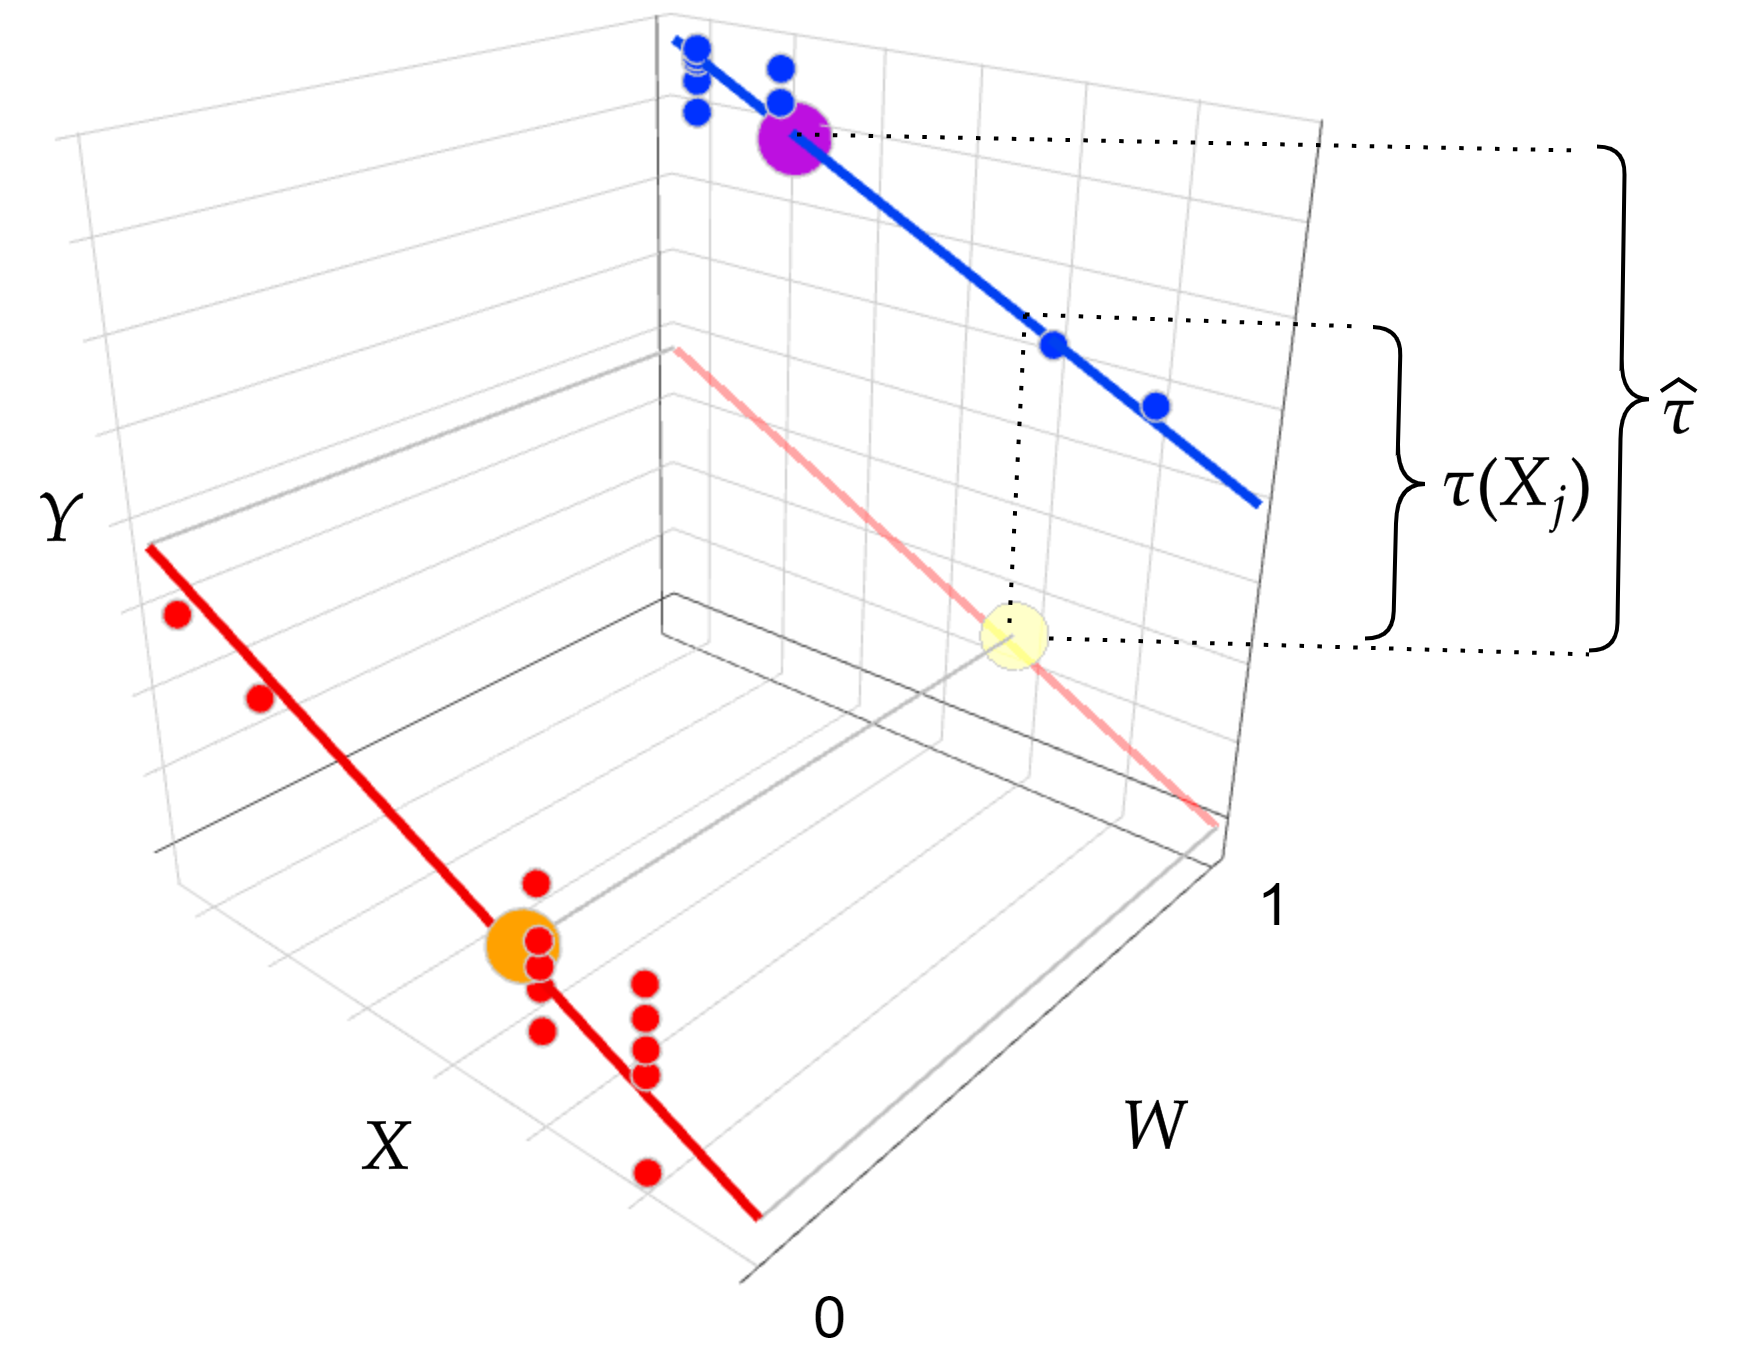
\includegraphics[width=0.55\linewidth]{sections/images/propensity.png}
    \caption{Illustration of covariate balance of propensity score (An example with linear dependence)}
\end{figure}

\begin{point}
    Statistical Inference to Propensity Score
\end{point}

Property of propensity score:
\begin{align}
    \Delta _\mathrm{tc}:= \mathbb{E}\left[ e(X)|W=1 \right] - \mathbb{E}\left[ e(X) |W=0\right]=\dfrac{var(e(X))}{p(1-p)}\\
    var(e(X))=\mathbb{E}\left[ \left(\dfrac{f_\mathrm{t}(X)-f_\mathrm{c}(X)  }{pf_\mathrm{t}(X)+(1-p)f_\mathrm{c}(X)}\right)^2 \right]\cdot p^2(1-p)^2   
\end{align}
\begin{itemize}[topsep=2pt,itemsep=0pt]
    \item Propensity Score test can be accessed by
\begin{align}
    &\hat{\Delta }_\mathrm{tc}^\ell = \dfrac{\bar{\ell}_\mathrm{t}-\bar{\ell}_\mathrm{c}  }{\sqrt{(s^2_{\ell,\mathrm{t} }+s^2_{\ell,\mathrm{c} } )/2}}\sim t_{N-2},\quad \ell(x)=\ln\left(\dfrac{e(x)}{1-e(x)}\right)=\mathrm{logistic}(x) \\
    &\hat{\Delta }_\mathrm{tc}^\ell =0\leftrightsquigarrow \Delta _\mathrm{tc}=0\leftrightsquigarrow var(e(X))=0\leftrightsquigarrow f_\mathrm{t}(x)=f_\mathrm{c}(x)  
\end{align}
    \item Estimate $ \hat{e}(X_i) $
    \begin{itemize}[topsep=2pt,itemsep=0pt]
        \item For categorical $ X $ with small $ |\mathcal{X}| $, estimation
        \begin{align}
            \hat{e}(x)=\dfrac{N(X_j)}{N} 
        \end{align}
        \item (Kernel) logistic regression is sometimes useful\footnote{Instruction of Kernel logistic regression see \autoref{SubSubSectionKernelRegression}.}
        \begin{align}
             \hat{e}(x)=\hat{\mathbb{P}}\left( W_i=1|X_i=x;\beta  \right)=\dfrac{e^{x'\beta }}{1+e^{x'\beta }} 
        \end{align}
    \end{itemize}
    
\end{itemize}

    







\begin{point}
    Useful Methods to Induce Propensity Score in Estimation
\end{point}
\begin{itemize}[topsep=2pt,itemsep=0pt]
    \item Weighting: using the modulation of $ e(x) $ on $ \mathbb{P}\left( W|X \right)  $
    \begin{align}\label{EqaPropensityScoreWeighting}
        \begin{cases}
            \mathbb{E}\left[ \dfrac{Y_i^\mathrm{obs}\cdot W_i }{e(X_i)} \right]=\mathbb{E}\left[ \dfrac{\mathbb{E}\left[ Y_i(1)|X_i \right]\mathbb{E}\left[ W_i|X_i \right]  }{e(X_i)} \right]=\mathbb{E}\left[ Y_i(1) \right]\\
            \mathbb{E}\left[ \dfrac{Y_i^\mathrm{obs}\cdot (1-W_i) }{1-e(X_i)} \right]=\mathbb{E}\left[ \dfrac{\mathbb{E}\left[ Y_i(0)|X_i \right]\mathbb{E}\left[ 1-W_i|X_i \right]  }{1-e(X_i)} \right]=\mathbb{E}\left[ Y_i(0) \right]
        \end{cases} 
    \end{align}
    to \textit{weight} estimators through $ X $: Horvitz-Thompson Estimator \index{Horvitz-Thompson Estimator}
    \begin{align}
        \hat{\tau}^\mathrm{HT} = & \dfrac{1}{N}\sum_{i=1}^N\dfrac{W_iY^\mathrm{obs}_i }{\hat{e}(X_i)}-\dfrac{1}{N}\sum_{i=1}^N\dfrac{(1-W_i)Y^\mathrm{obs}_i }{1-\hat{e}(X_i)}=\dfrac{1}{N}\sum_{i=1}^N\dfrac{(W_i-e(X_i))\cdot Y^\mathrm{obs}_i }{e(X_i)\cdot (1-e(X_i))} \\
        \hat{\tau}^\mathrm{HT,mod} = & \sum_{i=1}^N \lambda _iW_iY^\mathrm{obs}_i-\sum_{i=1}^N\lambda _i(1-W_i)Y^\mathrm{obs}_i ,\quad \lambda _i=\begin{cases}
            \dfrac{1/\hat{e}(X_i)}{\sum_{k=1}^NW_i /\hat{e}(X_j)},&W_i=1\\
            \dfrac{1/(1-\hat{e}(X_i))}{\sum_{k=1}^N  (1-W_i)/(1-\hat{e}(X_k))},&W_i=0
        \end{cases}  
    \end{align}
    where the modification version is used to avoid extreme $ \hat{e} $ value.

    The Horvitz-Thompson estimator is linked to stratified Neyman estimator \autoref{EqaNeymanEstimatorStratified} as
    \begin{align}
         \hat{\tau}^\mathrm{strata}=\sum_{j=1}^Jq(j)\hat{\tau}(j)= \dfrac{1}{N} \sum_{i=1}^N \tilde{e} _iW_iY^\mathrm{obs}_i-\sum_{i=1}^N\tilde{e} _i(1-W_i)Y^\mathrm{obs}_i ,\quad \tilde{e} _i=\begin{cases}
            \mathbb{I}_{S_i=j}\dfrac{1}{N_\mathrm{t}(j)/N(j) },&W_i=1\\
            \mathbb{I}_{S_i=j}\dfrac{1}{N_\mathrm{c}(j/N(j)) },&W_i=0
         \end{cases}
    \end{align}
    where $ \tilde{e }_i $ is the propensity score for each strata.
    \item Blocking / Stratifying according to $ X $, and then follows similar idea as SRE. (Because $ S(X_i) $ is still a covariate.)
    \item Matching `similar' data points. e.g. for each data point $ (W_i=1,Y_i,X_i) $, select in $ \mathcal{D}_{W=1-W_i=0} $ for units with small distance $ d(X_i,X) $ as $ \mathcal{M}_i $, and have a matching data
    \begin{align}
        \{(W_i=1,Y_i^\mathrm{obs} ,X_i,\mathcal{M}_i)\},\quad \mathcal{M}_i=\{(W_j=0,Y_j,X_j)\}_{d(X_i,X_j)\text{ small}} 
    \end{align}
    and then
    \begin{align}
        \hat{\tau} =\dfrac{1}{N_\mathrm{t} }\sum_{i:W_i=1}\left(Y_i^\mathrm{obs}-\bar{Y}_{\mathcal{M}_i} \right)
    \end{align}
\end{itemize}


\subsection{Pearl Causal Bayesian Framework}
\index{Pearl Causal Bayesian Framework}\index{Bayesian Network}
    Pearl Bayesian Framework\footnote{Also called Bayesian Network / Belief Network / Directed Acyclic Graphical (DAG) Model.} (Judea Pearl, 1995) uses causal information on a graph to construct inference. 

    
\subsubsection{Causal Bayesian Network}
The language of \textit{Graph} is used to describe the causal relations. 

\begin{point}
    Directed Acyclic Graph
\end{point}

In Pearl's causal network we focus on \textbf{Directed Acyclic Graphs} (DAGs) \index{DAG (Directed Acyclic Graph)}. Here are some key notions:
\begin{itemize}[topsep=2pt,itemsep=0pt]
    \item[$ \color{red}\vartriangleright  $] DAG is a graph in which all edges are directed, and no path is a loop (acyclic).
    \item[$ \color{blue}\vartriangleright  $] \textbf{Graph} $ \mathcal{G}$ is composed of a set of \textbf{Vertices}  / Nodes $\mathcal{V} $ and the \textbf{Edge}s $ \mathcal{E} $ connecting them; $\mathcal{G} = \left\{\mathcal{E},\mathcal{V}\right\} $.
    \item Adjacency: Two vertices $ v_i ,\,v_j$ are adjacent if they are linked by an edge $ e_{ij} $.
    \item \textbf{Path} : A (non-intersecting) routine tracing through edges to connect two vertices. 
    \item[$ \color{blue}\vartriangleright $] \textbf{Direction}  of edges: two vertices are connected by directed edge, pointing from the first to the second, say the following meta $ X\to Y $. 
    \begin{figure}[H]
        \centering          
        \begin{tikzpicture}
            \GraphInit[vstyle=Dijkstra]
            \SetGraphUnit{0.8}
            \Vertex[x=0, y=0, L=$ X $]{1}
            \Vertex[x=2, y=0, L=$ Y $]{2}

    
            \tikzset{LabelStyle/.style={fill = white},
            EdgeStyle/.style={-stealth}}
            \Edge(1)(2)
        \end{tikzpicture}
        \end{figure}
    in which $ X $ is a \textbf{parent} of $ Y $ and $ Y $ is a children of $ X $. Parent of note $ v_i $ is denoted $ pa_i $
    \item \textbf{Skeleton} : The graph with all direction removed (looks like a graph with only nodes and line, without arrow).
    \item[$ \color{blue}\vartriangleright $]  \textbf{Acyclic}: a graph without loop is acyclic. The structure is naturally required to make the causal structure healthy by clearly distinguish cause from effect.
\end{itemize}

\begin{point}
    Bayesian Network
\end{point}

A probability distribution $ \mathbb{P}\left( X_1,X_2,\ldots,X_n \right) $ on vertices of graph has factorization given by conditional probability:
\begin{align}
    \mathbb{P}\left( X_1,\ldots,X_n \right) = &\mathbb{P}\left( X_{i_1}|X_{i_2},\ldots \right)\mathbb{P}\left( X_{i_2}|X_{i_3},\ldots \right)\ldots\mathbb{P}\left( X_{i_{n-1}}|X_{i_n} \right) \mathbb{P}\left( X_n \right)    
\end{align}
in which indices $ \{i_1,i_2,\ldots,i_n\} $ can be any reshuffle of $ \{1,2,\ldots,n\} $. But if we attach a graph on the probability to guide the factorization, the shuffle has to following some order, and form of conditional probability follows the Markov parents on DAG:
\begin{align}
    \mathbb{P}\left( X_1,\ldots,X_n \right)=\prod_{i}\mathbb{P}\left( X_i|pa_i \right)
\end{align}
the r.v. sequence is \textbf{causal ordering} if $ X_i $ only dependent on $ X_{j:j<i} $, i.e. $ pa_i\subset \{X_1,\ldots,X_{i-1}\} $.

Here's an example of Markov factorization on a DAG graph:




    \begin{center}
    \begin{minipage}{0.7\linewidth}
        \begin{align}
            \mathbb{P}\left( X_1,X_2,X_3,X_4,X_5 \right) = & \mathbb{P}\left( X_5|X_4 \right) \mathbb{P}\left( X_1,X_2,X_3,X_4 \right) \\
            =&\mathbb{P}\left( X_5|X_4 \right) \mathbb{P}\left( X_4|X_2,X_3 \right) \mathbb{P}\left( X_1,X_2,X_3 \right) \\
            =&\mathbb{P}\left( X_5|X_4 \right) \mathbb{P}\left( X_4|X_2,X_3 \right) \mathbb{P}\left( X_3|X_1 \right) \mathbb{P}\left( X_2|X_1 \right) \mathbb{P}\left( X_1 \right)  \quad\,       
        \end{align}
    \end{minipage}
    \begin{tikzpicture}[baseline={([yshift = 0ex]current bounding box.center)}]
        \GraphInit[vstyle=Dijkstra]
        \SetGraphUnit{1.3}
        
        \Vertices[Lpos=-45]{circle}{3,1,2,4}
        \SO[unit = 1.4](4){5}

        \tikzset{LabelStyle/.style={fill = white},
        EdgeStyle/.style={-stealth}}

        \Edge(1)(2)
        \Edge(1)(3)
        \Edge(3)(4)
        \Edge(2)(4)
        \Edge(4)(5)
      \end{tikzpicture}
    \end{center}

\begin{point}
    Basic structures in a DAG 
\end{point}

Starting from triplets in DAG as the key elements in a graph.
\begin{itemize}[topsep=2pt,itemsep=0pt]
    \item Chain $ X\to Y\to Z $, in which $ Y $ is the \textit{mediator}. We have
    \begin{align}
        \mathbb{P}\left( X,Z|Y \right)=&\dfrac{\mathbb{P}\left( X \right) \mathbb{P}\left( Y|X \right) \mathbb{P}\left( Z|Y \right) }{\mathbb{P}\left( Y \right) }=\mathbb{P}\left( X|Y \right) \mathbb{P}\left( Z|Y \right) 
    \end{align}
    i.e. we have a conditional independency in chain $ X\independent Z|Y $
    \item Fork $ X\leftarrow Y\rightarrow Z $. We have
    \begin{align}
        \mathbb{P}\left( X,Z|Y \right) = \dfrac{\mathbb{P}\left( Y \right) \mathbb{P}\left( X|Y \right) \mathbb{P}\left( Z|Y \right) }{\mathbb{P}\left( Y \right) }=\mathbb{P}\left( X|Y \right) \mathbb{P}\left( Z|Y \right)   
    \end{align}
    i.e. we have a conditional independency in chain $ X\independent Z|Y $
    \item Collider $ X \to Y \leftarrow Z $. In the collider, $ X\independent Z $ marginally, but given $ Y $ are conditionally dependent. If there is no edge between $ X $ and $ Z $, it's also called $ v $-structure.\index{$ v $-structure@v-structure}
\end{itemize}

\begin{center}
    \begin{minipage}{0.3\linewidth}
        \begin{figure}[H]
        \centering            
            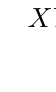
\begin{tikzpicture}[baseline={([yshift = -3ex]current bounding box.center)}]
            \GraphInit[vstyle=Dijkstra]
            \SetGraphUnit{0.8}
            \Vertex[x=0, y=0, L=$ X $]{1}
            \Vertex[x=1.5, y=0, L=$ Y $]{2}
            \Vertex[x=3, y=0, L=$ Z $]{3}

            \tikzset{LabelStyle/.style={fill = white},
            EdgeStyle/.style={-stealth}}
    
            \Edge(1)(2)
            \Edge(2)(3)
        \end{tikzpicture}            
        \caption{Chain}
        \end{figure}
    \end{minipage}\quad\begin{minipage}{0.3\linewidth}
        \begin{figure}[H]
        \centering            
        \begin{tikzpicture}
            \GraphInit[vstyle=Dijkstra]
            \SetGraphUnit{0.8}
            \Vertex[x=0, y=0, L=$ X $]{1}
            \Vertex[x=1, y=1.73, L=$ Y $]{2}
            \Vertex[x=2, y=0, L=$ Z $]{3}

    
            \tikzset{LabelStyle/.style={fill = white},
            EdgeStyle/.style={-stealth}}
    
            \Edge(2)(1)
            \Edge(2)(3)
        \end{tikzpicture}        
        \caption{Fork}
        \end{figure}
    \end{minipage}\quad\begin{minipage}{0.3\linewidth}
        \begin{figure}[H]
        \centering          
        \begin{tikzpicture}
            \GraphInit[vstyle=Dijkstra]
            \SetGraphUnit{0.8}
            \Vertex[x=0, y=0, L=$ X $]{1}
            \Vertex[x=1, y=-1.73, L=$ Y $]{2}
            \Vertex[x=2, y=0, L=$ Z $]{3}

    
            \tikzset{LabelStyle/.style={fill = white},
            EdgeStyle/.style={-stealth}}
    
            \Edge(1)(2)
            \Edge(3)(2)
        \end{tikzpicture}
        \caption{Collider}
        \end{figure}
    \end{minipage}
\end{center}


\begin{point}
    d-Separation\index{d-Separation}
\end{point}

d-separation in a graph is directional-separation of two vertices.

\begin{itemize}[topsep=2pt,itemsep=0pt]
    \item Blocked path: a path $ p $ from $ X $ to $ Y $ is blocked by $ \{Z\} $ if for all triplets along the path:
    \begin{itemize}[topsep=2pt,itemsep=0pt]
        \item \textbf{In} $ Z $: the middle point of all chains and forks; and
        \item \textbf{Not In} $ Z $: the middle point itself of collider, and its descendants
    \end{itemize}
    \item d-separation: $ X $ is d-deparated from $ Y $ given $ Z $ if all paths $ p_{X\leadsto Y} $ are blocked by $ Z $.
        
\end{itemize}

    

\begin{point}
    Markov Compatibility\index{Markov Compatibility}
\end{point}

Markov compatibility is a match between DAG and probability distribution, a description of how $ \mathcal{G} $ represents $ \mathbb{P}\left( \, \cdot \,  \right)  $.

A textbook definition is given as:
\begin{quote}
    If a probability distribution $ \mathbb{P}\left( \, \cdot \,  \right)  $ admits a factorization $ \mathbb{P}\left( X \right) = \prod_{i}\mathbb{P}\left( X_i|pa_i \right)  $ relative to DAG $ \mathcal{G} $, then $ \mathbb{P} $ is \textit{Markov Compatible} relative to $ \mathcal{G} $.
\end{quote}

Here `admits' means that d-separation on graph finds its corresponding conditional probability.
\begin{align}
    X\independent _\mathcal{G} Y|Z\Rightarrow  X\independent _\mathbb{P} Y|Z
\end{align}

Markov compatibility means that we can generate data following $ \mathbb{P} $ using $ \mathcal{G} $ as `Blueprint'.

Related notions and comments:

\begin{itemize}[topsep=2pt,itemsep=0pt]
    \item I-Map\index{I-map (Independence Map)}: is a set of conditional inpendence statements read out from $ \mathcal{G} $. If $ X $ and $ Y $ are d-separated by $ Z $ in $ \mathcal{G} $ (denoted $ X\independent_\mathcal{G} Y|Z $), then we should have $ X\independent_{mathbb{P}} Y |Z$ in \textbf{every} $ \mathbb{P} $ distribution compatible with $ \mathcal{G} $.
    \begin{align}
         I(\mathcal{G})=\left\{ (X\independent_\mathcal{G}Y|Z):\, (X\independent_\mathbb{P}Y|Z) \,\forall \mathbb{P}\text{ compatible with }\mathcal{G}  \right\}
    \end{align}
    \item From I-Map we can have definition of I-equivalence: i.e. if $ \mathcal{G}_1 $ and $ \mathcal{G}_2 $ yield the same I-map $ I(\mathcal{G}_1)=I(\mathcal{G}_2) $.
    \item Note that Markov compatible states that $ X\independent _\mathcal{G} Y|Z\Rightarrow  X\independent _\mathbb{P} Y|Z $ but not reversely, which means that $ I(\mathcal{G})\subset I(\mathbb{P}) $
    \item An concrete example: two r.v. are independently generated $ \mathbb{P}\left( X,Y \right) =\mathbb{P}\left( X\right)\mathbb{P}\left( Y \right) $, i.e. $ I(\mathbb{P})= X\independent_\mathbb{P} Y $. All the following graphs are markov compatible:
    \begin{itemize}[topsep=2pt,itemsep=0pt]
        \item $ \mathcal{G}_0: X\,\, Y $, in which $ I(\mathcal{G}_0) = X\independent _\mathcal{G} Y $
        \item $ \mathcal{G}_1: X\to Y $, in which $ I(\mathcal{G}_1) = \emptyset  $
        \item $ \mathcal{G}_2: X\leftarrow Y $, in which $  I(\mathcal{G}_2) = \emptyset $
    \end{itemize}
    (because they all have $ I(\mathcal{G}_i)\subset I(\mathbb{P}) $)
    \item Perfect I-map: if $ I(\mathcal{G})=I(\mathbb{P}) $.
    \item \textbf{Observational Equivalence}\index{Observational Equivalence}: A set of graphs are observational equivalent / belong to the same equivalent class if they encode the same conditional independencies. 
    
    Note that the key causal structures in DAGs are chain, fork, and collider; in which chain and fork imply the same conditional independence while collider is different. i.e.
    \begin{align}
        X\to Y\to Z,\qquad X\leftarrow Y\leftarrow Z,\qquad X\leftarrow Y \to Z 
    \end{align}
    are observational equivalent by encoding $ X\independent Z|Y $.
    
    The above argument gives the hint for identifying observational equivalent graphs:
    \begin{itemize}[topsep=2pt,itemsep=0pt]
        \item Having the same skeleton
        \item Having the same set of colliders.
    \end{itemize}

   
    Here's an example of observational equivalent graphs:
    \begin{center}
        \begin{minipage}{0.23\linewidth}
            \begin{figure}[H]
            \centering            
                \begin{tikzpicture}[baseline={([yshift = -3ex]current bounding box.center)}]
                    \GraphInit[vstyle=Dijkstra]
                    \SetGraphUnit{1.2}
                    
                    \Vertices[Lpos=-45]{circle}{3,1,2,4}
                    \SO[unit = 1.4](4){5}

                    \tikzset{LabelStyle/.style={fill = white},
                    EdgeStyle/.style={thick}}
            
                    \Edge(1)(2)
                    \Edge(1)(3)
            
                    \tikzset{LabelStyle/.style={fill = white},
                    EdgeStyle/.style={-stealth}}
            
                    \Edge(3)(4)
                    \Edge(2)(4)
                    \Edge(4)(5)
            \end{tikzpicture}     
            $$ \text{(Partial) Skeleton} $$       
            % \caption{aa}
            \end{figure}
        \end{minipage}\quad
        \begin{minipage}{0.23\linewidth}
            \begin{figure}[H]
            \centering            
                \begin{tikzpicture}[baseline={([yshift = -3ex]current bounding box.center)}]
                    \GraphInit[vstyle=Dijkstra]
                    \SetGraphUnit{1.2}
                    
                    \Vertices[Lpos=-45]{circle}{3,1,2,4}
                    \SO[unit = 1.4](4){5}
            
                    \tikzset{LabelStyle/.style={fill = white},
                    EdgeStyle/.style={-stealth}}
            
                    \Edge(1)(2)
                    \Edge(1)(3)
                    \Edge(3)(4)
                    \Edge(2)(4)
                    \Edge(4)(5)
            \end{tikzpicture}     
            $$ \mathcal{G}_1 $$       
            % \caption{aa}
            \end{figure}
        \end{minipage}\quad        \begin{minipage}{0.23\linewidth}
            \begin{figure}[H]
            \centering            
                \begin{tikzpicture}[baseline={([yshift = -3ex]current bounding box.center)}]
                    \GraphInit[vstyle=Dijkstra]
                    \SetGraphUnit{1.2}
                    
                    \Vertices[Lpos=-45]{circle}{3,1,2,4}
                    \SO[unit = 1.4](4){5}
            
                    \tikzset{LabelStyle/.style={fill = white},
                    EdgeStyle/.style={-stealth}}
            
                    \Edge(1)(2)
                    \Edge(3)(1)
                    \Edge(3)(4)
                    \Edge(2)(4)
                    \Edge(4)(5)
            \end{tikzpicture}  
            $$  \mathcal{G}_2 $$        
            % \caption{aa}
            \end{figure}
        \end{minipage}\quad        \begin{minipage}{0.23\linewidth}
            \begin{figure}[H]
            \centering            
                \begin{tikzpicture}[baseline={([yshift = -3ex]current bounding box.center)}]
                    \GraphInit[vstyle=Dijkstra]
                    \SetGraphUnit{1.2}
                    
                    \Vertices[Lpos=-45]{circle}{3,1,2,4}
                    \SO[unit = 1.4](4){5}
            
                    \tikzset{LabelStyle/.style={fill = white},
                    EdgeStyle/.style={-stealth}}
            
                    \Edge(2)(1)
                    \Edge(1)(3)
                    \Edge(3)(4)
                    \Edge(2)(4)
                    \Edge(4)(5)
            \end{tikzpicture} 
            $$  \mathcal{G}_3  $$
            % \caption{aa}
            \end{figure}
        \end{minipage}
    \end{center}
\end{itemize}

\begin{point}
    Causality on Bayesian Network
\end{point}

Recall that in Rubin's Potential Outcome Framework, causality was induced by counterfactual side of potential outcomes $ Y^\mathrm{mis} = Y(1-W)  $. In Bayesian Network framework, causality is induced by \textbf{intervention}, in formulas expressed by $ do(\, \cdot \, ) $ operator, e.g.
\begin{align}
    \mathbb{P}\left( X |do(Z=z) \right)  
\end{align}
where $ Z\subset X  $ is the set to conduct intervention on. Intervention would remove all `incoming' edges to $ Z $, as illustrated below an example of $ do(3=...) $:

\begin{center}
    \begin{minipage}{0.23\linewidth}
        \begin{figure}[H]
        \centering            
            \begin{tikzpicture}[baseline={([yshift = -3ex]current bounding box.center)}]
                \GraphInit[vstyle=Dijkstra]
                \SetGraphUnit{1.2}
                
                \Vertices[Lpos=-45]{circle}{3,1,2,4}
                \SO[unit = 1.4](4){5}
                \tikzset{LabelStyle/.style={fill = white},
                EdgeStyle/.style={-stealth}}
                \Edge(1)(2)
                \Edge(1)(3)        
                \Edge(3)(4)
                \Edge(2)(4)
                \Edge(4)(5)
        \end{tikzpicture}     
        $$ \text{Original }\mathcal{G} $$       
        % \caption{aa}
        \end{figure}
    \end{minipage}\quad $ \xrightarrow[]{do(=...)\text{ intervention}}  $
    \begin{minipage}{0.23\linewidth}
        \begin{figure}[H]
        \centering            
            \begin{tikzpicture}[baseline={([yshift = -3ex]current bounding box.center)}]
                \GraphInit[vstyle=Dijkstra]
                \SetGraphUnit{1.2}
                
                \Vertices[Lpos=-45]{circle}{3,1,2,4}
                \SO[unit = 1.4](4){5}
        
                \tikzset{LabelStyle/.style={fill = white},
                EdgeStyle/.style={-stealth}}
        
                \Edge(1)(2)
                \Edge(3)(4)

                \Edge(2)(4)
                \Edge(4)(5)
        \end{tikzpicture}     
        $$ \text{Interventional }\mathcal{G} $$       
        % \caption{aa}
        \end{figure}
    \end{minipage}
\end{center}

Since intervention produces different subgraphs, we can obtain causality by comparing the probability distribution. e.g. in the simplest instance $ X\to Y $ v.s. $ X\leftarrow Y $, intervention $ do(X=x) $ yields $ x\to Y $ and $ X\quad Y $, respectively, which have different observational outcome.

\textbf{Causal Bayesian Network} (CBN)\index{CBN (Causal Bayesian Network)} is a DAG $ \mathcal{G} $ compatible with $ \mathcal{P} $, if 
\begin{itemize}[topsep=2pt,itemsep=0pt]
    \item Notation: here $ \mathcal{P}=\left\{ \mathbb{P}\left( X|do(Z=z) \right):\,\forall Z\subset X  \right\} $ is the set of all interventional probability distribution.
    \item $ \forall \mathcal{P}\ni \mathbb{P}\left( X|do(Z=z) \right)   $ is compatible with $ \mathcal{G} $
    \item $ \mathbb{P}\left( x_i|do(Z=z) \right)=1   $ if $ X_i\in Z $ and $ x_i=z_{\text{corresponding value}} $ ($ X_i=x_i $ is consistent with $ Z=z $)
    \item $ \mathbb{P}\left( X_i|pa_i \right)  $ is invariant to interventions not involving $ X_i $ itself.
\end{itemize}

Comments:
\begin{itemize}[topsep=2pt,itemsep=0pt]
    \item Note that intervention $ do(Z=z) $ cancels some edges, so it would only add newindependencies, which holds $ I(\mathcal{G})\subset I(\mathbb{P} ) $ (still compatible).
    \item With some intervention $ do(Z=z) $, the \textit{truncated} factorization of $ \mathbb{P}\left( \, \cdot \,  \right)  $ is
    \begin{align}
        \mathbb{P}\left( X | do(Z=z) \right)  =  \prod_{i:X_i\notin Z}\mathbb{P}\left( X_i|pa_i \right) 
    \end{align}
    
    
\end{itemize}

    

    








\subsubsection{Network Structure Learning}

\begin{point}
    IC/PC Algorithm\index{IC Algorithm (Inductive Causation Algorithm)}
\end{point}

IC/PC Algorithm (Inductive Causation Algorithm with Peter \& Clark Algorithm Refinement) is a constraint-based method. DAG is constructed through identifying conditional independencies.

Here illustrated with the following example with conditional independencies. Ground truth is shown on the right 

\begin{center}
    \begin{minipage}{0.4\linewidth}
        \begin{align}
            &X \not\!\!\mathop{\independent} R |\mathcal{S},\,\forall \mathcal{S}\subset\{Y,Z,W\}\\
            &X \not\!\!\mathop{\independent} Z |\mathcal{S},\,\forall \mathcal{S}\subset\{Y,R,W\}\\
            &X \not\!\!\mathop{\independent} Y |\mathcal{S},\,\forall \mathcal{S}\subset\{Z,R,W\}\\
            &Y \not\!\!\mathop{\independent} Z |\mathcal{S},\,\forall \mathcal{S}\subset\{X,R,W\}\\
            &Y \not\!\!\mathop{\independent} W |\mathcal{S},\,\forall \mathcal{S}\subset\{X,Z,R\}\\
            &X\independent W|Y\\
            &Y\independent R\\
            &Z\independent W|Y\\
            &Z\independent R|\{X,Y\}\\
            &W\independent R
        \end{align}
    \end{minipage}
    \begin{tikzpicture}[baseline={([yshift = 0ex]current bounding box.center)}]
        \GraphInit[vstyle=Dijkstra]
        \SetGraphUnit{1.3}
        
        \Vertex[x=0, y=0, L=$ R $]{R}
        \Vertex[x=1, y=-1, L=$ X $]{X}
        \Vertex[x=2, y=0, L=$ Y $]{Y}
        \Vertex[x=2, y=-2, L=$ Z $]{Z}
        \Vertex[x=3, y=-1, L=$ W $]{W}

        \tikzset{LabelStyle/.style={fill = white},
        EdgeStyle/.style={-stealth}}

        \Edge(R)(X)
        \Edge(Y)(X)
        \Edge(X)(Z)
        \Edge(Y)(Z)
        \Edge(Y)(W)

      \end{tikzpicture}
    \end{center}




\begin{enumerate}[topsep=2pt,itemsep=2pt]
    \item Learning Skeleton: For all paris $ (a,b)\in \mathcal{V}\times \mathcal{V} $:
    \begin{itemize}[topsep=2pt,itemsep=0pt]
        \item Connect $ a $, $ b $ iff no $ \mathcal{S}_{ab} $ such that $ a\independent b|S_{ab} $ can be found. i.e. $ a,\,b $ have an edge if $ a\not\!\!\mathop{\independent} b|\text{any set of other nodes} $.
    \end{itemize}
    \begin{center}
        \begin{minipage}{0.4\linewidth}
            \begin{align}
                &\color{red}X \not\!\!\mathop{\independent} R |\mathcal{S},\,\forall \mathcal{S}\subset\{Y,Z,W\}\\
                &\color{red}X \not\!\!\mathop{\independent} Z |\mathcal{S},\,\forall \mathcal{S}\subset\{Y,R,W\}\\
                &\color{red}X \not\!\!\mathop{\independent} Y |\mathcal{S},\,\forall \mathcal{S}\subset\{Z,R,W\}\\
                &\color{red}Y \not\!\!\mathop{\independent} Z |\mathcal{S},\,\forall \mathcal{S}\subset\{X,R,W\}\\
                &\color{red}Y \not\!\!\mathop{\independent} W |\mathcal{S},\,\forall \mathcal{S}\subset\{X,Z,R\}\\
                &X\independent W|Y\\
                &Y\independent R\\
                &Z\independent W|Y\\
                &Z\independent R|\{X,Y\}\\
                &W\independent R
            \end{align}
        \end{minipage}
        \begin{tikzpicture}[baseline={([yshift = 0ex]current bounding box.center)}]
            \GraphInit[vstyle=Dijkstra]
            \SetGraphUnit{1.3}
            
            \Vertex[x=0, y=0, L=$ R $]{R}
            \Vertex[x=1, y=-1, L=$ X $]{X}
            \Vertex[x=2, y=0, L=$ Y $]{Y}
            \Vertex[x=2, y=-2, L=$ Z $]{Z}
            \Vertex[x=3, y=-1, L=$ W $]{W}
    
            \tikzset{LabelStyle/.style={fill = white},
            EdgeStyle/.style={-, color = red}}
    
            \Edge(R)(X)
            \Edge(Y)(X)
            \Edge(X)(Z)
            \Edge(Y)(Z)
            \Edge(Y)(W)
    
          \end{tikzpicture}
        \end{center}
    
    
    \item $ v $-structure Orientation: For all $ (a,b) $ with common neighbour $ c $ but not adjacent, i.e. have $ a $-$ c $-$ b $
    \begin{itemize}[topsep=2pt,itemsep=2pt]
        \item If $ c\notin \mathcal{S}_{ab} $, then there is a v-structure $ a\to c\leftarrow b $
    \end{itemize}
    \begin{center}
        \begin{minipage}{0.4\linewidth}
            \begin{align}
                &\color{red}X \not\!\!\mathop{\independent} R |\mathcal{S},\,\forall \mathcal{S}\subset\{Y,Z,W\}\\
                &X \not\!\!\mathop{\independent} Z |\mathcal{S},\,\forall \mathcal{S}\subset\{Y,R,W\}\\
                &\color{red}X \not\!\!\mathop{\independent} Y |\mathcal{S},\,\forall \mathcal{S}\subset\{Z,R,W\}\\
                &Y \not\!\!\mathop{\independent} Z |\mathcal{S},\,\forall \mathcal{S}\subset\{X,R,W\}\\
                &Y \not\!\!\mathop{\independent} W |\mathcal{S},\,\forall \mathcal{S}\subset\{X,Z,R\}\\
                &X\independent W|Y\\
                &\color{red}Y\independent R\\
                &Z\independent W|Y\\
                &Z\independent R|\{X,Y\}\\
                &W\independent R
            \end{align}
        \end{minipage}
        \begin{tikzpicture}[baseline={([yshift = 0ex]current bounding box.center)}]
            \GraphInit[vstyle=Dijkstra]
            \SetGraphUnit{1.3}
            
            \Vertex[x=0, y=0, L=$ R $]{R}
            \Vertex[x=1, y=-1, L=$ X $]{X}
            \Vertex[x=2, y=0, L=$ Y $]{Y}
            \Vertex[x=2, y=-2, L=$ Z $]{Z}
            \Vertex[x=3, y=-1, L=$ W $]{W}
    
            \tikzset{LabelStyle/.style={fill = white},
            EdgeStyle/.style={-}}
            \Edge(X)(Z)
            \Edge(Y)(Z)
            \Edge(Y)(W)
            \tikzset{LabelStyle/.style={fill = white},
            EdgeStyle/.style={-stealth, color = red}}
            \Edge(R)(X)
            \Edge(Y)(X)
          \end{tikzpicture}
        \end{center}
    
    
    \item Meek's rule Orientation: orient as many edges as possible subject to:
    \begin{itemize}[topsep=2pt,itemsep=0pt]
        \item Alternative direction yields new $ v $-structure
        \begin{center}
            \begin{tikzpicture}[baseline={([yshift = 0ex]current bounding box.center)}]
                \GraphInit[vstyle=Dijkstra]
                \SetGraphUnit{1.3}
                
                \Vertex[x=0, y=0, L=$ R $]{R}
                \Vertex[x=1, y=-1, L=$ X $]{X}
                \Vertex[x=2, y=0, L=$ Y $]{Y}
                \Vertex[x=2, y=-2, L=$ Z $]{Z}
                \Vertex[x=3, y=-1, L=$ W $]{W}
        
                \tikzset{LabelStyle/.style={fill = white},
                EdgeStyle/.style={-}}
                \Edge(Y)(Z)
                \Edge(Y)(W)
                \tikzset{LabelStyle/.style={fill = white},
                EdgeStyle/.style={-stealth}}
                \Edge(R)(X)
                \Edge(Y)(X)
                \tikzset{LabelStyle/.style={fill = white},
                EdgeStyle/.style={dashed, -stealth}}
                \Edge(Z)(X)
              \end{tikzpicture}
              $ \qquad  $\begin{tikzpicture}[baseline={([yshift = 0ex]current bounding box.center)}]
                \GraphInit[vstyle=Dijkstra]
                \SetGraphUnit{1.3}
                
                \Vertex[x=0, y=0, L=$ R $]{R}
                \Vertex[x=1, y=-1, L=$ X $]{X}
                \Vertex[x=2, y=0, L=$ Y $]{Y}
                \Vertex[x=2, y=-2, L=$ Z $]{Z}
                \Vertex[x=3, y=-1, L=$ W $]{W}
        
                \tikzset{LabelStyle/.style={fill = white},
                EdgeStyle/.style={-}}
                \Edge(Y)(Z)
                \Edge(Y)(W)
                \tikzset{LabelStyle/.style={fill = white},
                EdgeStyle/.style={-stealth}}
                \Edge(R)(X)
                \Edge(Y)(X)
                \tikzset{LabelStyle/.style={fill = white},
                EdgeStyle/.style={-stealth,color=red}}
                \Edge(X)(Z)
              \end{tikzpicture}
            \end{center}
        \item Alternative direction yields cycle (acyclic rule is of more priority)
        \begin{center}
            \begin{tikzpicture}[baseline={([yshift = 0ex]current bounding box.center)}]
                \GraphInit[vstyle=Dijkstra]
                \SetGraphUnit{1.3}
                
                \Vertex[x=0, y=0, L=$ R $]{R}
                \Vertex[x=1, y=-1, L=$ X $]{X}
                \Vertex[x=2, y=0, L=$ Y $]{Y}
                \Vertex[x=2, y=-2, L=$ Z $]{Z}
                \Vertex[x=3, y=-1, L=$ W $]{W}
        
                \tikzset{LabelStyle/.style={fill = white},
                EdgeStyle/.style={-}}
                \Edge(Y)(W)
                \tikzset{LabelStyle/.style={fill = white},
                EdgeStyle/.style={-stealth}}
                \Edge(R)(X)
                \Edge(Y)(X)
                \Edge(X)(Z)
                \tikzset{LabelStyle/.style={fill = white},
                EdgeStyle/.style={dashed, -stealth}}
                \Edge(Z)(Y)
              \end{tikzpicture}
              $ \qquad  $\begin{tikzpicture}[baseline={([yshift = 0ex]current bounding box.center)}]
                \GraphInit[vstyle=Dijkstra]
                \SetGraphUnit{1.3}
                
                \Vertex[x=0, y=0, L=$ R $]{R}
                \Vertex[x=1, y=-1, L=$ X $]{X}
                \Vertex[x=2, y=0, L=$ Y $]{Y}
                \Vertex[x=2, y=-2, L=$ Z $]{Z}
                \Vertex[x=3, y=-1, L=$ W $]{W}
        
                \tikzset{LabelStyle/.style={fill = white},
                EdgeStyle/.style={-}}
                \Edge(Y)(W)
                \tikzset{LabelStyle/.style={fill = white},
                EdgeStyle/.style={-stealth}}
                \Edge(R)(X)
                \Edge(Y)(X)
                \Edge(X)(Z)
                \tikzset{LabelStyle/.style={fill = white},
                EdgeStyle/.style={-stealth,color=red}}
                \Edge(Y)(Z)
              \end{tikzpicture}
            \end{center}
    \end{itemize}
\end{enumerate}

The above procedure can produce identify the DAG up to its observational equivalent class.




\begin{point}
    Search and Score Methods
\end{point}

We could also simply search in the space of all possible networks and select the one scoring the highest. Some frequently used metrics include AIC and BIC
\begin{align}
    \mathrm{AIC}=&-2\log \mathbb{P}\left( \mathcal{G}|\hat{\theta }  \right) + 2\mathrm{dof}_\mathcal{G} \\
    \mathrm{BIC}=&-2\log \mathbb{P}\left( \mathcal{G}|\hat{\theta } \right) +\log n \mathrm{dof}_\mathcal{G}   
\end{align}



\subsubsection{Network Parameter Learning}
Basically, parameter learning (given BN strucure) is simply estimating edge weights, denoted $ \varTheta $. Two basic methods are 
\begin{itemize}[topsep=2pt,itemsep=0pt]
    \item Bayesian approach
    \begin{align}
        \mathop{\arg\max}\limits_{\varTheta}\mathbb{P}(\varTheta|\mathcal{D})  
    \end{align}
    \item Frequentist approach, e.g. with MLE loss+penalty form
    \begin{align}
         \mathop{\arg\min}\limits_{\varTheta}-\log\mathbb{P}\left( \mathcal{D}|\varTheta \right) + \lambda P(\varTheta)  
    \end{align}

    A trivial solution for categorical variables is 
    \begin{align}
        \hat{\theta}_{ij\vec{k}}=\hat{\mathbb{P}}(X_i=j|pa_{i}=\vec{k})=\dfrac{N_{ijk}}{N_{i\cdot k}},\,\forall j=1,\ldots,J_{i} ,\,\,\forall i\in\mathcal{V}
    \end{align}
    
    
\end{itemize}

    
\subsubsection{Average Causal Effect Estimation}
    Average Causal Effects on BN are defined in terms of $ do(\, \cdot \, ) $ operator,
    \begin{align}
        \mathrm{ACE}(Y|H):= \mathbb{E}\left[ Y|do(H=h_1) \right]-\mathbb{E}\left[ Y|do(H=h_2) \right]    
    \end{align}
    Calculation of ACE given known BN relies on $ do $-calculus. A $ do(\, \cdot \, ) $ operator would cancal all edges pointing to the vertex, i.e. produce a modified graph $ \mathcal{G}_{do(\, \cdot \, )} $, what we need to estimate is the probability in the modified graph. 
    \begin{align}
         \mathbb{E}_{\mathcal{G}}\left[ Y|do(H) \right] \twoheadleftarrow  \mathbb{P}_{\mathcal{G}}\left( Y|do(H) \right) \twoheadleftarrow  \mathbb{P}_{\mathcal{G}_{do(H)}}\left( Y \right) \xleftarrow[]{do\text{-calculus}} \mathbb{P}_{\mathcal{G}}\left( \mathbf{X} \right)  \twoheadleftarrow \mathcal{D}ata
    \end{align}

    \begin{center}
        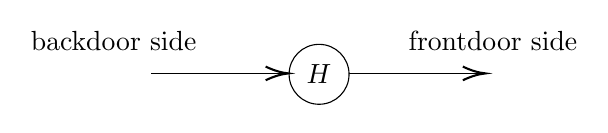
\begin{tikzpicture}[x=0.75pt,y=0.75pt,yscale=-1,xscale=1]
        %uncomment if require: \path (0,300); %set diagram left start at 0, and has height of 300
        
        %Straight Lines [id:da46339212876531755] 
        \draw    (206.33,126.77) -- (270.33,126.77) ;
        \draw [shift={(272.33,126.77)}, rotate = 180] [color={rgb, 255:red, 0; green, 0; blue, 0 }  ][line width=0.75]    (10.93,-3.29) .. controls (6.95,-1.4) and (3.31,-0.3) .. (0,0) .. controls (3.31,0.3) and (6.95,1.4) .. (10.93,3.29)   ;
        %Straight Lines [id:da21292385445434125] 
        \draw    (301.33,126.77) -- (365.33,126.77) ;
        \draw [shift={(367.33,126.77)}, rotate = 180] [color={rgb, 255:red, 0; green, 0; blue, 0 }  ][line width=0.75]    (10.93,-3.29) .. controls (6.95,-1.4) and (3.31,-0.3) .. (0,0) .. controls (3.31,0.3) and (6.95,1.4) .. (10.93,3.29)   ;
        
        % Text Node
        \draw    (287.13, 127.2) circle [x radius= 14.44, y radius= 14.44]   ;
        \draw (287.13,127.2) node  [xslant=-0.03]  {$H$};
        % Text Node
        \draw (147,105) node [anchor=north west][inner sep=0.75pt]   [align=left] {backdoor side};
        % Text Node
        \draw (329,105) node [anchor=north west][inner sep=0.75pt]   [align=left] {frontdoor side};
        
        
        \end{tikzpicture}
    \end{center}

    \begin{point}
        $ do $-Calculus
    \end{point}
    \begin{itemize}[topsep=2pt,itemsep=0pt]
        \item Module invariant
        \begin{align}
            \mathbb{P}\left( X_i=x_i\big| do(PA_i=pa_i) \right) = \mathbb{P}\left( X_i=x_i\big| PA_i=pa_i \right)  
        \end{align}
        \item[$ \color{blue}\vartriangleright  $]\textbf{ The Adjustment Formula} \index{Adjustment Formula}
        \begin{align}
            \mathbb{P}\left( Y=y\big| do(X=x) \right) =& \sum_{z\in\{ pa_y \}} \mathbb{P}\left( Y=y\big| X=x, PA_y=z \right)\mathbb{P}\left( PA_y=z \right)  \\
            =& \sum_{z\in\{pa_y\}}\dfrac{\mathbb{P}\left( X=x, Y=y,PA_y=z \right) }{\mathbb{P}\left( X=x\big| PA_y=z \right) } 
        \end{align}
        in which we use the Markovian factorization on $ \mathcal{G} $
        \begin{align}
            \mathbb{P}\left( X,Y,PA_y \right) = \mathbb{P}\left( Y|X,PA_y \right)\mathbb{P}\left( X|PA_y \right)   \mathbb{P}\left( PA_y \right)  
        \end{align}
        with $ X $ considered as assignment mechanism, $ Z $ considered as covariates, the formula shares the same idea as \autoref{EqaPropensityScoreWeighting}.
        
        Through adjustment formula, we could obtain ACE from observed data (without intervention $ \leadsto $ with intervention).
        
        \fbox{\begin{minipage}{0.98\linewidth}
            \makebox[2em][]{}\textbf{Example:} assessing $ Y|do(X=x) $, in which $ PA_y=\{X,Z\} $ with $ X $ being fixed by $ do(X=x) $.
            \begin{align}
                \mathbb{P}\left( Y=y\big| do(X=x) \right) = & \sum_{z\in\{z\}} \mathbb{P}\left( Y\big| X=x,Z=z \right) \mathbb{P}\left( Z=z \right) 
            \end{align}

            \begin{center}
            \begin{minipage}{0.25\linewidth}
                \centering
                Before Intervention $ do(X) $\\
                \begin{tikzpicture}[baseline={([yshift = 0ex]current bounding box.center)}]
                \GraphInit[vstyle=Dijkstra]
                \SetGraphUnit{1.3}
                
                \Vertex[x=0, y=0, L=$ X $]{X}
                \Vertex[x=1, y=1, L=$ Z $]{Z}
                \Vertex[x=2, y=0, L=$ Y $]{Y}

                \tikzset{LabelStyle/.style={fill = white},
                EdgeStyle/.style={-stealth}}
        
                \Edge(X)(Y)
                \Edge(Z)(Y)
                \Edge(Z)(X)
        
            \end{tikzpicture}
            \end{minipage}
            $ \Rightarrow  $
            \begin{minipage}{0.25\linewidth}
                \centering
                After Intervention $ do(X) $\\
                \begin{tikzpicture}[baseline={([yshift = 0ex]current bounding box.center)}]
                \GraphInit[vstyle=Dijkstra]
                \SetGraphUnit{1.3}
                
                \Vertex[x=0, y=0, L=$ X $]{X}
                \Vertex[x=1, y=1, L=$ Z $]{Z}
                \Vertex[x=2, y=0, L=$ Y $]{Y}

                \tikzset{LabelStyle/.style={fill = white},
                EdgeStyle/.style={-stealth}}
        
                \Edge(X)(Y)
                \Edge(Z)(Y)
        
            \end{tikzpicture}
            \end{minipage}

            \end{center}
        \end{minipage}}
        \item[$ \color{blue}\vartriangleright  $] \textbf{Backdoor criterion}  \index{Backdoor Criterion}
        
        Given $ (X,Y) $ in BN, a `backdoor set' $ \bm{Z} $ is one such that $ \bm{Z} $:
        \begin{itemize}[topsep=2pt,itemsep=0pt]
            \item Blocks \textbf{all} paths with arrow onto $ X $ (i.e. backdoor side of $ X $ is blocked by $ \bm{Z} $)
            \item $ \bm{Z} $ contains \textbf{no}  descendants of $ X $
        \end{itemize}
        
        then we could use the backdoor variable set $ \bm{Z} $ to have the \textbf{backdoor adjustment} of $ Y|do(X) $ as  
        \begin{align}
            \mathbb{P}\left( Y=y|do(X=x) \right)=\sum_{\bm{z}}\mathbb{P}\left( Y=y|X=x,\bm{Z}=\bm{z} \right)\mathbb{P}\left( \bm{Z}=\bm{z} \right)    
        \end{align}
        The selection of backdoor set $ \bm{Z} $ is not unique. e.g. sometimes due to observablility problem we could only obtain Partial DAG $ \big/ $ have multiple methods to block the path, then we could pick proper nodes to form the backdoor set.

        \fbox{\begin{minipage}{0.98\linewidth}
            \makebox[2em][]{}\textbf{Example:} assessing $ Y|do(X=x) $, where $ Z $ is an observable while $ W $ is a hidden unobservable.
            \begin{align}
                \mathbb{P}\left( Y=y\big| do(X=x) \right) = & \sum_{z\in\{z\}} \mathbb{P}\left( Y\big| X=x,Z=z \right) \mathbb{P}\left( Z=z \right) 
            \end{align}
    
            \begin{center}
            \begin{tikzpicture}[baseline={([yshift = 0ex]current bounding box.center)}]
                \GraphInit[vstyle=Dijkstra]
                \SetGraphUnit{1.3}
                
                \Vertex[x=0, y=0, L=$ X $]{X}
                \Vertex[x=0, y=1.5, L=$ Z $]{Z}
                \Vertex[x=2, y=0, L=$ Y $]{Y}
                \Vertex[x=2, y=1.3, L=$ W $]{W}
    
                \tikzset{LabelStyle/.style={fill = white},
                EdgeStyle/.style={-stealth}}
        
                \Edge(X)(Y)
                \Edge(Z)(W)
                \Edge(Z)(X)
                \Edge(W)(Y)
                
        
                \end{tikzpicture}
                \end{center}
            \end{minipage}}

            \fbox{\begin{minipage}{0.98\linewidth}
                \makebox[2em][]{}\textbf{Example:} assessing $ Y|do(X=x) $.
                \begin{align}
                    \mathbb{P}\left( Y=y\big| do(X=x) \right) = & \sum_{(z,z_1)\in\{(z,z_1)\}} \mathbb{P}\left( Y\big| X=x,Z=z,Z_1=z_1 \right) \mathbb{P}\left( Z=z,Z_1=z_1 \right)\\
                    =&\sum_{(z,z_2)\in\{(z,z_2)\}} \mathbb{P}\left( Y\big| X=x,Z=z,Z_2=z_2 \right) \mathbb{P}\left( Z=z,Z_2=z_2 \right)\\
                    =& \sum_{(z,z_1,z_2)\in\{(z,z_1,z_2)\}} \mathbb{P}\left( Y\big| X=x,Z=z,Z_1=z_1,Z_2=z_2 \right)\\
                    &\qquad \cdot \mathbb{P}\left( Z=z,Z_1=z_1,Z_2=z_2 \right)
                \end{align}
        
                \begin{center}
                \begin{tikzpicture}[baseline={([yshift = 0ex]current bounding box.center)}]
                    \GraphInit[vstyle=Dijkstra]
                    \SetGraphUnit{1.3}
                    
                    \Vertex[x=0, y=0, L=$ X $]{X}
                    \Vertex[x=1, y=1, L=$ Z $]{Z}
                    \Vertex[x=2, y=0, L=$ Y $]{Y}
                    \Vertex[x=-1, y=1.5, L=$ Z_1 $]{z1}
                    \Vertex[x=3, y=1.5, L=$ Z_2 $]{z2}
        
                    \tikzset{LabelStyle/.style={fill = white},
                    EdgeStyle/.style={-stealth}}
            
                    \Edge(X)(Y)
                    \Edge(Z)(Y)
                    \Edge(Z)(X)
                    \Edge(z1)(X)
                    \Edge(z1)(Z)
                    \Edge(z2)(Z)
                    \Edge(z2)(Y)
                    
            
                    \end{tikzpicture}
                    \end{center}
                    \qquad i.e. we could adjust for either $ (Z,Z_1) $ or $ (Z,Z_2) $ or $ (Z,Z_1,Z_2) $ as the backdoor set.
                \end{minipage}
                }
        \item[$ \color{blue}\vartriangleright  $] \textbf{Frontdoor criterion} 
        
        Given $ (X,Y) $ in BN, a `frontdoor set' $ \bm{Z} $ is one such that $ \bm{Z} $:
        \begin{itemize}[topsep=2pt,itemsep=0pt]
            \item Intercepts \textbf{all} paths from $ X $ to $ Y $ (i.e. frontdoor side of $ X $ is intercepted $ \bm{Z} $)
            \item \textbf{No} unblocked backdoor path from $ X $ to $ Z $\footnote{backdoor path from $ X $ to $ Z $ means containing a backdoor arrow of $ X $, e.g. in the example, $ X\leftarrow W\to Y\leftarrow Z $, is blocked.}
            \item \textbf{All} backdoor paths from $ Z $ to $ Y $ blocked by $ X $
        \end{itemize}
        then we could use the frontdoor variable set $ \bm{Z} $ to have the frontkdoor adjustment of $Y |do(X)$ as\index{Frontdoor Adjustment}
        \begin{align}
            \mathbb{P}\left( Y=y\big| do(X=x) \right) = & \sum_{z}\mathbb{P}\left( Z=z|X=x \right)\sum_{x'}\mathbb{P}\left( Y=y|X'=x',Z=z \right)\mathbb{P}\left( X'=X' \right)  
        \end{align}
        
        \fbox{\begin{minipage}{0.98\linewidth}
            \makebox[2em][]{}\textbf{Example:} assessing $ Y|do(X=x) $.
            \begin{align}
                \mathbb{P}\left( Y=y\big| do(X=x) \right) = & \sum_{z}\mathbb{P}\left( Z=z|X=x \right)\sum_{x'}\mathbb{P}\left( Y=y|X'=x',Z=z \right)\mathbb{P}\left( X'=X' \right)   
            \end{align}
    
            \begin{center}
            \begin{tikzpicture}[baseline={([yshift = 0ex]current bounding box.center)}]
                \GraphInit[vstyle=Dijkstra]
                \SetGraphUnit{1.3}
                
                \Vertex[x=0, y=0, L=$ X $]{X}
                \Vertex[x=1.2, y=0, L=$ Z $]{Z}
                \Vertex[x=2.4, y=0, L=$ Y $]{Y}
                \Vertex[x=1.2, y=1.2, L=$ W $]{W}
    
                \tikzset{LabelStyle/.style={fill = white},
                EdgeStyle/.style={-stealth}}
        
                \Edge(X)(Z)
                \Edge(Z)(Y)
                \Edge(W)(X)
                \Edge(W)(Y)
                
        
                \end{tikzpicture}
                \end{center}
                The derivation is using backdoor adjustment twice
                \begin{align}
                    \begin{cases}
                        \mathbb{P}\left( Y=y|do(X=x) \right) = \sum_{z}\mathbb{P}\left( Y=y|do(Z=z) \right)\mathbb{P}\left( Z=z|do(X=x) \right)\\  
                        \mathbb{P}\left( Y=y|do(Z=z) \right)=\sum_{x}\mathbb{P}\left( Y=y|Z=z,X=x \right) \mathbb{P}\left( X=x \right)\\
                        \mathbb{P}\left( Z=z|do(X=x) \right)   =\mathbb{P}\left( Z=z|X=x \right) 
                    \end{cases} 
                \end{align}
                
                
            \end{minipage}}
        \item[$ \color{red}\vartriangleright  $] General Rules of $ do $-calculus
    \end{itemize}
    
        



    
















    % \begin{center}
    %     \begin{tikzpicture}
    %         \GraphInit[vstyle=Dijkstra]
    %         \SetGraphUnit{0.8}
            
    %         \Vertex[x=4.5, y=2, L= $ X_1 $]{1}
    %         \Vertex[x=0, y=0, L=$ X_2 $]{2}
    %         \Vertex[x=3, y=-2, L=$ X_3 $]{3}
    %         \Vertex[x=6, y=0, L=$ X_4 $]{4}
    %         \Vertex[x=9, y=0, L=$ X_5 $]{5}
    %         \Vertex[x=3, y=-4, L=$ X_6 $]{6}
    
    %         \tikzset{LabelStyle/.style={fill = white},
    %         EdgeStyle/.style={-stealth}}
    
    %         \Edge(1)(2)
    %         \Edge(1)(5)
    %         \Edge(2)(3)
    %         \Edge(4)(3)
    %         \Edge(4)(5)
    %         \Edge(3)(6)
    %       \end{tikzpicture}
    % \end{center}
% \newpage

% \section{应用随机过程部分}
\begin{center}
    Instructor: Pengkun Yang 
\end{center}

% \subsection{Review of Probability}



\subsection{Properties of Stochastic Process}
% (Or sometimes called random process)

\subsubsection{Basic Concepts}
Some basic concepts about stochastic process / random process are introduced in \autoref{SubSectionStochasticProcessForTimeSeries}. Here's a brief recap.

A stochastic process is a mapping
\begin{align}
     \{X_t:t\in\mathcal{T}\}:\, \Omega \mapsto \mathcal{T}\times \mathbb{R}
\end{align}

\begin{itemize}[topsep=2pt,itemsep=0pt]
    \item For given $ t \in\mathcal{T}$, $ X_t(\, \cdot \, ) $ is a r.v. defined on $ \Omega  $.
    \item For given $ \omega \in \Omega  $, $ X_\cdot (\omega ) $ is a function on $ \mathcal{T} $, which is called sample path.\index{Sample Path}
\end{itemize}

According to the continuity of index Fourier Transformset $ \mathcal{T} $ and sample path values, Stochastic process can be categorized in discrete / continuous Time + discrete / continuous State processes.

Some functions of stochastic processes include
\begin{itemize}[topsep=2pt,itemsep=0pt]
    \item Mean function:
    \begin{align}
        \mu _X(t)=\mathbb{E}\left[ X_t \right]  
    \end{align}
    \item AutoCovariance function (ACVF):
    \begin{align}
        \gamma _{s,t}:=cov(X_s,X_t)
    \end{align}
    \item AutoCorrelation function (ACF):
    \begin{align}
        \rho _{s,t}:=corr(X_s,X_t)=\dfrac{\gamma _{s,t}}{\sqrt{\gamma _{s,s}\gamma _{t,t}}} 
    \end{align}
    \item $ n^\mathrm{th}  $ order CDF:
    \begin{align}
        F_{X,n}(x_1,t_1;x_2,t_2;\ldots;x_n,t_n)=\mathbb{P}\left( X_{t_1}\leq x_1,\,X_{t_2}\leq x_2,\ldots,\,X_{t_n}\leq x_n \right)  
    \end{align}
   
\end{itemize}

% \begin{point}
%     Some Examples 
% \end{point}

% \begin{itemize}[topsep=2pt,itemsep=0pt]
%     \item Trajectory of horizontal projectile motion with random initial height $ A\sim f_A $ and initial velocity $ B\sim f_B $:
%     \begin{align}
%         Y_t=-\dfrac{1}{2}gt^2+B(\omega _B)t+A(\omega _A)
%     \end{align}

%     with 
%     \begin{align}
%         \gamma _{s,t}=1+st,\quad \rho _{s,t}=\dfrac{1+st}{\sqrt{(1+s^2)(1+t^2)}}  
%     \end{align}
    
    
%     \item 
    
    
% \end{itemize}

    


\subsubsection{Properties of Discrete Time Markov Chain}\label{SubSubSectionDTMC}
A basic case for Markov Chain is Discrete Time Markov Chain (DTMC)\index{DTMC (Discrete Time Markov Chain)}

\begin{point}
    Notations and Properties of DTMC
\end{point}
\begin{itemize}[topsep=2pt,itemsep=0pt]
    \item State: denote the state space / phase space of DTMC as
    \begin{align}
        X_n\in \mathcal{S} 
    \end{align}
    \item Conditional Independency: 
    \begin{align}
         \mathbb{P}\left( X_{n+1}\big|X_0,X_1,\ldots,X_n \right)=\mathbb{P}\left( X_{n+1}\big|X_n \right)  
    \end{align}
    
    
    \item State transition and transition probability matrix:
    \begin{align}
        P^{(k)}=\left\{P^{(k)}_{ij}\right\}=\left\{ \mathbb{P}\left( X_{k+1}=j\big| X_{k}=i \right)  \right\},\quad i,j\in \mathcal{S}
    \end{align}
    transition pr matrix $ P $ is called a (row) stochastic matrix, with
    \begin{align}
        0\leq P^{(k)}_{ij}\leq 1,\quad \sum_{j}P^{(k)}_{ij}=1 
    \end{align}

    \item Time homogeneity: transition probability is independent of step / time
    \begin{align}
        P^{(k)}=P,\quad \forall k 
    \end{align}
    we usually focus on time-homogeneous DTMC.
    
    \item State diagram: a useful way to visualize DTMC, in which vertices / nodes for states and edges / arrows for transition. Here's an example of `Mickey Mouse' diagram with six states:
    \begin{center}
        $
            P=\begin{pNiceMatrix}[first-row,first-col]
                &0&1&2&3&4&5\\
                0&&4/9&&&&5/9\\
                1&1/9&4/9&4/9&&&\\
                2&&4/9&4/9&1/9&&\\
                3&&&4/9&&5/9&\\
                4&&&&&&1\\
                5&&&&&&1
            \end{pNiceMatrix}\qquad \quad\bm{\leftrightharpoons }
        $
        \begin{tikzpicture}[baseline={([yshift = -5ex]current bounding box.center)}]
            \GraphInit[vstyle=Dijkstra]
            \SetGraphUnit{2}
            
            \Vertices[Lpos=45]{circle}{0,1,2,3,4,5}

            \tikzset{LabelStyle/.style={fill = white},
            EdgeStyle/.style={-stealth}}
            \Loop[dist = 2cm, dir = NOEA, label = 4/9](1)
            \Loop[dist = 2cm, dir = NOWE, label = 4/9](2)

            \tikzset{EdgeStyle/.style={-stealth, bend right}}
            \Edge[label = 4/9](0)(1)
            \Edge[label = 1/9](1)(0)
            \Edge[label = 4/9](1)(2)
            \Edge[label = 4/9](2)(1)
            \Edge[label = 1/9](2)(3)
            \Edge[label = 4/9](3)(2)
            \Edge[label = 5/9](3)(4)
            \Edge[label = 1](4)(5)

            \tikzset{EdgeStyle/.style={-stealth, bend left}}
            \Edge[label = 5/9 ](0)(5)
          \end{tikzpicture}
        \end{center}
\end{itemize}

\begin{point}
    Stationary Distribution\index{Stationary Distribution}\index{Equilibrium}
\end{point}

    State transition between steps are like jumping in state diagram. Denote $ \pi(k) $ the probability distribution at step $ k $, then a transition is
        \begin{align}
            \pi({k+1})=\pi(k)P^{(k)}=\pi(k)P 
        \end{align}

        A stationary distribution / equilibrium of DTMC is the eigen distribution of transition matrix
        \begin{align}
            \pi^*=\pi^*P=\pi^*P^i,\,\forall i 
        \end{align}
        
        A sufficient condition for stationary state is the detailed balance condition\index{Detailed Balance Condition}
        \begin{align}
            &\pi^*_i=\sum_{j}\pi^*_jP_{ji}\\
            \Leftrightarrow&\pi^*\sum_{j\neq i}P_{ij}=\pi^*_i(1-P_{ii})=\sum_{j\neq i}\pi^*jP_{ji}\\
            \Leftarrow&\color{red}\pi_iP_{ij}=\pi_jP_{ji}
        \end{align}

        Some concepts related to stationary distribution
    \begin{itemize}[topsep=2pt,itemsep=0pt]
        \item Reachable: we can arrive at $ j $ starting from $ i $, denoted $ i\leadsto j $
        \begin{align}
            \exists n<\infty s.t. \mathbb{P}\left( X_n=j|X_0=i \right) > 0 
        \end{align}

        Sometimes I use the notation $ i\xrightarrow[]{k}j  $ for `reaching $ j $ in $ k $ steps from $ i $'
        \item Irreducible\index{Irreducible}: every state is reachable from any other states
        \begin{align}
            i\leadsto j,\,\forall i,j\in\mathcal{S} 
        \end{align}
        
        \item Periodic: the period $ d_i $ for state $ i $ is the greatest common divisor (GCD)\index{GCD (Greatest Common Divisor)} of step-to-come-back.
        \begin{align}
            d_i:=\gcd\left\{ n:\mathbb{P}\left( X_n=i|X_0=i \right)>0  \right\} 
        \end{align}

        Irreducible DTMC has the same period for all states.

        % \begin{proof}
            For any two states $ i $, $ j $, with periods $ d_i $, $ d_j $. Then $ d_i $ contains the following process:
            \begin{align}
                \{i\xrightarrow[]{k_1}j\xrightarrow[]{m\times d_j}j\xrightarrow[]{k_n}i \} ,\quad m\in\mathbb{N}
            \end{align}
            there are infinite elements. then
            \begin{align}
                d_i=\mathrm{cd} \left\{ k_1+k_2+md_j;m=0,1,2,\ldots \right\} \Rightarrow d_j=\text{multiple of }d_i
            \end{align}
         
            With the argument applied to all state pairs $ (i,j)\in\mathcal{S}\times \mathcal{S} $, obviously $ d_i=d,\,\forall i\in\mathcal{S} $
        % \end{proof}
        \item Aperiodic\index{Aperiodic}: is the case that $ d_i=1 $, i.e. possible to come back anytime. For irreducible DTMC, if one state is aperiodic, then all are.        
        
        Naturally if a node is self looped $ P_{ii}>0 $ (e.g. node 1 or 2 in `Mickey Mouse' loops back with pr $ 4/9 $), then all the states are aperiodic.
        \item Sojourn Time\index{Sojourn Time} $ T_i $: is the time to stay at the state
        \begin{align}\label{EqaDTMCSojournTime}
            T_i\sim \mathrm{Geo}(1-P_{ii})  
        \end{align}
        \item Classification of States. 
        
        Denote Hitting Time (without itself include) $ \tau_i^+ $ and its mean 
        \begin{align}
            \tau_i^+:=&\min\{k\geq 1:X_k=i\}\\
            \mu _i:=&\mathbb{E}\left[ \tau_i^+|X_0=i \right] 
        \end{align}
        
        \begin{itemize}[topsep=2pt,itemsep=0pt]
            \item Recurrent State
            \begin{align}
                \mathbb{P}\left( \tau_i^+<\infty|X_0=i    \right)=1  
            \end{align}
            in which 
            \begin{itemize}[topsep=2pt,itemsep=0pt]
                \item Positive Recurrent\index{Positive Recurrent State}
                \begin{align}
                    \mu _i<\infty 
                \end{align}
                \item Null Recurrent
                \begin{align}
                    \mu _i=\infty 
                \end{align}

                An example:
                \begin{center}
                \begin{tikzpicture}
                \GraphInit[vstyle=Dijkstra]
                \SetGraphUnit{2}
                    \tikzset{VertexStyle/.style = {
                        shape = rectangle,
                        color = black,
                        text = black,
                        inner sep = 2pt,
                        outer sep = 2pt,
                        draw}}
                    \Vertices{line}{1,2,3,4}
                    \EA[L=$3^k-1$](4){8}
                    \EA[L=$ 3^k $](8){9}
                    \EA[L=$ 3^k+1 $](9){10}
                    \tikzset{VertexStyle/.style = {
                        shape = circle,
                        color = white,
                        text = black,
                        minimum size = 23pt,
                        draw}}
                
                    \EA[L=...,unit=0.8 ](4)(5)
                    \EA[L=...,unit=1.2 ](10)(11)

                    \tikzset{EdgeStyle/.style = {->,bend left,thick}}
                    \tikzset{LabelStyle/.style = {fill=white}}

                    \Edge[label=1/2](3)(1)
                    \Edge[label=1/2](9)(1)

                    \Edge[label=1/2](3)(4)
                    \Edge[label=1/2](9)(10)

                    \Edge[label=1](1)(2)
                    \Edge[label=1](8)(9)
                    \Edge[label=1](2)(3)

                \end{tikzpicture}
                \end{center}

                where 
                \begin{align}
                    \mu _1=\mathbb{E}\left[ \tau_1^+|X_0=1 \right]=\sum_{i=1}^\infty \left(\dfrac{3}{2}\right)^i\to\infty   
                \end{align}
                
                

            \end{itemize} 
            \item Transient State
            \begin{align}
                \mathbb{P}\left( \tau_i^+<\infty|X_0=i    \right)<1 
            \end{align}
        \end{itemize}
        
            
    \end{itemize}
    
\begin{point}
    DTMC: Irreducible \& Aperiodic \& Positive Recurrent $ \Rightarrow  $ Unique Stationary Distribution $ \pi^* $ Exists
\end{point}

Given irreducible \& aperiodic DTMC, we have 

\begin{itemize}[topsep=2pt,itemsep=0pt]
    \item All states have the same state classification: null recurrent / positive recurrent / transient.
    \item if all states are positive recurrent $ \mu _i<\infty $, then stationary distribution exists.
    \begin{align}
        \lim_{n\to \infty}\dfrac{1}{n}\sum_{l=1}^n(P^l)_{ij}=\dfrac{1}{\mu _i}\Rightarrow \pi_i(\infty)=(\pi(0)P^\infty)_i= \dfrac{1}{\mu _i},\, \forall \pi(0)
    \end{align}
    \item Further if states are positive recurrent $ \mu _i<\infty $, then stationary distribution.
\begin{align}
    \pi^*=\dfrac{1}{\mu _i} 
\end{align}

    The proof is a little bit complicated, but an intuition is direct. For a realization of Markov Process $ \{X_t\}_{t=1}^\infty $, in which $ \{X_{i_1},X_{i_2},\ldots\} $ is the set that $ X_t=i $ for any given $ i $, and $ \{u_{i_1},u_{i_2},\ldots\}=\{i_1-i_2,i_3-i_2,\ldots\} $ is the time-btw-event, i.e. $ u_{i_j}\sim_{i.i.d.} \sim \tau^+_i|X_0=i,\,\forall j$. Then
    \begin{align}
        \lim_{n\to\infty}\sum_{t=1}^n\mathbb{I}_{X_t=i}=\lim_{k\to\infty}\dfrac{k}{u_{i_1}+u_{i_2}+\ldots+u_{i_k}}=\dfrac{1}{\mathbb{E}\left[ \tau_{i}^+|X_0=i \right] }=\dfrac{1}{\mu _i}
    \end{align}

    \index{Ergodicity}
    Comment: Ergodicity = irreducible \& aperiodic condition. It \textit{creates link between phase structure and time structure}, which makes $ \bar{u} $ (time-average) converge in an appropriate sense to $ \mu _i $ (phase-average).
    
    
    
\end{itemize}

Some algorithm about Markov Chain see \autoref{SubSubSectionMCMCAlgorithm}.


\begin{point}
    Concrete examples of DTMC
\end{point}
\begin{itemize}[topsep=2pt,itemsep=0pt]
    \item \hyperlink{RandomWalk}{Random Walk}
    \item \hyperlink{GamblersModel}{Gambler's Model}
    \item \hyperlink{BranchingProcess}{Branching Process}
\end{itemize}






\subsubsection{Properties of Continuous Time Markov Chain}\label{SubSubSectionCTMC}
Another case of Markov Chain is Continuous Time Markov Chain (CTMC)\index{CTMC (Continuous Time Markov Chain)}

\begin{point}
    Notations and Properties of CTMC
\end{point}
\begin{itemize}[topsep=2pt,itemsep=0pt]
    \item Concepts of state and conditional independency are similar to DTMC
    \begin{align}
         \mathbb{P}\left( X_{t_{n+1}}\big|X_{t_0},X_{t_1},\ldots,X_{t_{n}} \right)=\mathbb{P}\left( X_{t_{n+1}}\big| X_{t_n} \right)  
    \end{align}
    \item Transition probability matrix
    \begin{align}
         H(s,t):=\{H_{ij}(s,t)\}=\{\mathbb{P}\left( X_{t}=j|X_{s}=i \right) \},\quad s<t
    \end{align}
    with a trivial case that $ H(t,t)=I $. State transition could be expressed by matrix $ H(s,t) $ as
    \begin{align}
        p(t)=p(s)H(s,t)
    \end{align}
    
    \item Chapman-Kolmogorov Equation\index{Chapman-Kolmogorov Equation}
    \begin{align}
        H(r,t)=H(r,s)H(s,t),\quad r<s<t 
    \end{align}
    \item Time homogeneity: transition probability is independent of time interval:
    \begin{align}
        H(s,t)=H(0,t-s) 
    \end{align}
    \item Generator of time homogeneous CTMC: The \textbf{Transition Rate Matrix} is\index{Transition Rate Matrix} 
    \begin{align}
        Q:=\lim_{\delta \to 0}\dfrac{H(\delta )-H(0)}{\delta },\quad H(\delta )=I+\delta Q+o(\delta ) 
    \end{align}
    with Chapman-Kolmogorov Equation we could see that $ Q $ is the generator of the transition matrix \index{Generator}(group)
    \begin{align}
        H(t)\mathop{=}\limits_{t=n\delta }\lim_{n\to\infty}H(\delta )^n=\lim_{n\to\infty}\left(I+\dfrac{t}{n}Q\right)^{n}=e^{Qt}  
    \end{align}
    And note that $ H(t) $ has 1 row-sum, $ \sum_{j}\left(e^{Qt}\right)_{ij}=1 $:
    \begin{align}
        0=\dfrac{\mathrm{d}\sum_{j}\left(e^{Qt}\right)_{ij}}{\mathrm{d}t^{}}=&\sum_{j,k}Q_{ik} \left(e^{Qt}\right)_{kj}=\sum_{k}Q_{ik}=0\\
        \Rightarrow Q_{ii}=&-\sum_{k\neq i}Q_{ik},\quad \forall i
    \end{align}
    i.e. generator $ Q $ has 0 row-sum.

    Comment: with Gershgorin Circle Theorem\index{Gershgorin Circle Theorem} \footnote{Detail see \url{https://v1ncent19.github.io/texts/DiagonalDominant/}.}, $ Q $ as a diagonal dominant matrix, is negative definite, which guarentee the convergence of $ H(t)=e^{Qt}<\infty $
    \item Kolmogorov Forward Equation\index{Kolmogorov Forward}:\footnote{Note that $ Q $ and $ e^{Qt} $ are commutable
    \begin{align}
         Qe^{Qt}=Q\sum_{i=0}^\infty\dfrac{Q^it^i}{i!}=e^{Qt}Q
    \end{align}
    }
    \begin{align}
        \dot{p}(t)=\dfrac{\mathrm{d}^{} p(0)e^{Qt}}{\mathrm{d}t}=p(0)e^{Qt}Q=p(t)Q
    \end{align}

    Kolmogorov forward could also be deduced for some other specifically defined event / probability. 
    \item Stationary Distribution\index{Stationary Distribution}\index{Equilibrium}: with $ \dot{\pi}^*=0 $ in Kolmogorov forward, stationary distribution of CTMC:
    \begin{align}
         \pi^*=\pi^*H(t),\,\forall t\Leftrightarrow \pi^*Q=0
    \end{align}
    thus yield the detailed balance in CTMC version:
    \begin{align}
         \color{red}\pi^*Q=0\Leftarrow \pi^*_iq_{ij}=0,\,\forall i,j
    \end{align}
    \item Dynamics of CTMC\index{Sojourn Time}: Each step (say, $ 0\leadsto t\leadsto t+\delta  $) in state transitions in CTMC could be decomposed in two sub-steps:
    \begin{align}
        \begin{cases}
            \text{Sojourn}:&T_i\sim \mathbb{P}\left(t: X_\tau=i\,\forall 0\leq \tau\leq t\big| X_0=i \right)\\
            \text{Jump}:&p_{ij}^\mathrm{J}\sim  \mathbb{P}\left( X_{t+\delta}=j\big| X_t=i,X_{t+\delta }\neq i\right) 
        \end{cases}
    \end{align}
    which has the following dynamics
    \begin{align}
        \begin{cases}
            T_i\sim \varepsilon (-q_{ii})\\
            p_{ij}^\mathrm{J}=(\delta _{ij}-1)\dfrac{q_{ij}}{q_{ii}} 
        \end{cases} 
    \end{align}
    Where sojourn time $ T_i $ is a continuous correspondance of \ref{EqaDTMCSojournTime}. In both versions it is memoryless.
\end{itemize}

\begin{point}
    CTMC: Irreducible \& Non-explosive \& Positive Recurrent $ \Rightarrow  $ Unique Stationary Distribution $ \pi^* $
\end{point}

Given irreducible \& non-explosive CTMC, we have
\begin{itemize}[topsep=2pt,itemsep=0pt]
    \item All states have the same state classification: null recurrent / positive recurrent / transient
    \item Stationary distribution exists $ \Leftrightarrow $ all states are positive recurrent
    \begin{align}
        \lim_{t\to\infty}p_i(t)=\dfrac{1}{-q_{ii}\mu _i} = \pi^*_i
    \end{align}
\end{itemize}


\begin{point}
    Concrete examples of CTMC
\end{point}
\begin{itemize}[topsep=2pt,itemsep=0pt]
    \item \hyperlink{BrownianProcess}{Brownian Process}: CTMC with continuous states;
    \item \hyperlink{PoissonProcess}{Poisson Process}: CTMC with discrete states;
    \item 
\end{itemize}


\subsubsection{Independent Increment Process and Martingale}\label{SubSubSectionIndepedentProcess}

Motivation: Sometimes a process is a `summation of all past events'.

\begin{itemize}[topsep=2pt,itemsep=0pt]
    \item Independent Increment: Def. $ \{X_t\} $ a \textbf{independent increment process} if $ \forall t_0<t_1<\ldots<t_n $, $ \forall n $
\begin{align}
    X_{t_{n}}-X_{t_{n-1}}\independent X_{t_{n-1}}-X_{t_{n-2}} \independent \ldots\independent X_{t_1}-X_{t_0}
\end{align}
    \item Martingale: Def. $ \{X_t\}  $ a \textbf{Martingale} if $ \forall t_0<t_1<\ldots<t_n $, $ \forall n $
    \begin{align}
        \mathbb{E}\left[ X_{t_n}|X_{t_{n-1}},\ldots,X_{t_0} \right] = X_{t_{n-1}} 
    \end{align}
    with a technical condition of bounded expectation $ \mathbb{E}\left[ |X_t| \right] <\infty $.
    \item Martingale: Def. $ \{X_t\}  $ being a Martingale w.r.t. $ \{Y_t\} $ if
    \begin{align}
        \mathbb{E}\left[ X_{t_n}|Y_{t_{n-1}},\ldots,Y_{t_0} \right] = X_{t_{n-1}} 
    \end{align}
    with bounded expectation $ \mathbb{E}\left[ |X_t| \right] <\infty $.

    
\end{itemize}

\begin{point}
    Concrete examples of independent increment processes
\end{point}

\begin{itemize}[topsep=2pt,itemsep=0pt]
    \item \hyperlink{BrownianProcess}{Brownian Process}: homogeneous events, probabilistic increment.
    \item \hyperlink{PoissonProcess}{Poisson Process}: probabilistic events, homogeneous increment.
\end{itemize}




\subsubsection{Ergodicity}






\subsection{Useful Instances of Stochastic Processes}

\subsubsection{Random Walk}
\hypertarget{RandomWalk}{}

Random walk is a renewal process $ X_n $ with each step $ W_i $ takes value $ \pm 1 $\index{Random Walk}
\begin{align}
    X_n := X_0 +\sum_{i=1}^nW_i\quad W_i=\begin{cases}
        +1&\mathrm{w.p.}\, p\\
        -1&\mathrm{w.p.}\, q:=1-p  
    \end{cases}
\end{align}
where $ X_0=k $ is the initial position.

\begin{point}
    Simple Random Walk
\end{point}

Simple random walk is the case with no ends, i.e. $ X_n\in \mathbb{Z} $


\begin{itemize}[topsep=2pt,itemsep=0pt]
    \item State Diagram for Simple Random Walk
\begin{center}
    \begin{tikzpicture}
    \GraphInit[vstyle=Dijkstra]
    \SetGraphUnit{2}
        \tikzset{VertexStyle/.style = {
            shape = rectangle,
            color = black,
            text = black,
            inner sep = 2pt,
            outer sep = 2pt,
            draw}}
        \Vertex[L=$ k $]{0}
        \EA[L=$k+1$](0){1}
        \EA[L=$k+2$](1){2}
        \WE[L=$k-1$](0){10}
        \WE[L=$k-2$](10){20}
        \tikzset{VertexStyle/.style = {
            shape = circle,
            color = white,
            text = black,
            minimum size = 23pt,
            draw}}
        \EA[L=...,unit=1.9 ](2){3}
        \WE[L=...,unit=1.9 ](20){30}

        \tikzset{EdgeStyle/.style = {->,bend left,thick}}
        \tikzset{LabelStyle/.style = {fill=white}}

        \Edge[label=$ p $](30)(20)
        \Edge[label=$ p $](20)(10)
        \Edge[label=$ p $](10)(0)
        \Edge[label=$ p $](0)(1)
        \Edge[label=$ p $](1)(2)
        \Edge[label=$ p $](2)(3)

        \Edge[label=$ q $](20)(30)
        \Edge[label=$ q $](10)(20)
        \Edge[label=$ q $](0)(10)
        \Edge[label=$ q $](1)(0)
        \Edge[label=$ q $](2)(1)
        \Edge[label=$ q $](3)(2)


    \end{tikzpicture}
    \end{center}
    \item Parameters
    \begin{align}
        \begin{cases}
            \text{Mean Function}:\mu _n=k+n(2p-1)\\
            \text{Covariance}:\gamma _{m,n}=4pq\min\{m,n\}\\
            \text{CLT}:\dfrac{X_n-k-n(2p-1)}{\sqrt{4npq}}\xrightarrow[]{d} N(0,1)
        \end{cases} 
    \end{align}
    
    
\end{itemize}

\subsubsection{Gambler's Model}
\hypertarget{GamblersModel}{}
\index{Gambler's Model}

Gambler's model is the case with one/two ends, usually one of the ends is denoted $ 0 $, as Gambler's ruin, and the other denoted $ N $ as Gambler's success.

Reaching $ 0 $ or $ N $ stops the chain, so are called `absorbing state'.\index{Absorbing State}

\begin{itemize}[topsep=2pt,itemsep=0pt]
    \item State Diagram of Gambler's model with two ends
    \begin{center}
        \begin{tikzpicture}
        \GraphInit[vstyle=Dijkstra]
        \SetGraphUnit{2}
            \tikzset{VertexStyle/.style = {
                shape = rectangle,
                color = black,
                text = black,
                inner sep = 2pt,
                outer sep = 2pt,
                draw}}
            \Vertex[L=$ 0 $]{0}
            \EA[L=$1$](0){1}
            \EA[L=$2$](1){2}
            \tikzset{VertexStyle/.style = {
                shape = circle,
                color = white,
                text = black,
                minimum size = 23pt,
                draw}}
            \EA[L=$ \ldots $](2){3}
            \tikzset{VertexStyle/.style = {
                shape = rectangle,
                color = black,
                text = black,
                inner sep = 2pt,
                outer sep = 2pt,
                draw}}
            \EA[L=$ N-2 $](3){4}
            \EA[L=$ N-1 $](4){5}
            \EA[L=$ N $](5){6}

            \tikzset{LabelStyle/.style = {fill=white}}
            \Loop[dist = 1.2cm, dir = EA, label = 1](6)
            \Loop[dist = 1.2cm, dir = WE, label = 1](0)

    
            \tikzset{EdgeStyle/.style = {->,bend left,thick}}
            \tikzset{LabelStyle/.style = {fill=white}}
    
            \Edges[label = $ p $](1,2,3,4,5,6)
            \Edges[label = $ q $](5,4,3,2,1,0)
    
        \end{tikzpicture}
        \end{center}
    \item Gambler's Ruin / Success: Denote Hitting Time (allowing itself included)\index{Hitting Time} $\tau_i=\min\left\{ n\geq 0: X_n=i \right\} $, and  probability of ruin $ r_i $ and probability of success $ s_i $ respectively
    \begin{align}
        r_i:=&\mathbb{P}\left( X_{\tau_0}=0|X_0=i \right)\\
        s_i:=&\mathbb{P}\left( X_{\tau_N}=N|X_0=i \right)
    \end{align}
    with itertion relation
    \begin{align}
        s_i=p\cdot s_{i+1}+q\cdot s_{i-1},\quad s_0=0,\,s_N=1\\
        r_i=q\cdot r_{i+1}+p\cdot r_{i-1},\quad r_0=1,\,r_N=0 
    \end{align}

    we could get\footnote{For the case $ q=p=1/2 $, take the natural limit to get corresponding solution
    \begin{align}
        s_i=&\dfrac{k}{N}\\
        r_i=&1-\dfrac{k}{N}
    \end{align}
    }
    \begin{align}
        s_i=&\dfrac{1-(q/p)^i}{1-(q/p)^N}\\
        r_i=&\dfrac{(q/p)^i-(q/p)^N}{1-(q/p)^N}=1-s_i
    \end{align}
    \item Mean Hitting Time $ T_{i\leadsto \{0,N\}} $ for $ i\leadsto \{0,N\} $: $ T_{i\leadsto \{0,N\}}=\mathbb{E}\left[ \min\{\tau_{0},\tau_{N}\}|X_0=i \right]  $:
    \begin{align}
        T_{i\leadsto \{0,N\}}= p\left(1+T_{i+1\leadsto \{0,N\}}\right) + q\left(1+T_{i-1\leadsto \{0,N\}}\right),\quad T_{N\leadsto \{0,N\}}=T_{0\leadsto \{0,N\}}=0
    \end{align}
    solution
\begin{align}
    T_{i\leadsto\{0,N\}}=\dfrac{\left(1-(q/p)^i\right)(N-i)}{\left(1-(q/p)^N\right)(p-q)} 
\end{align}
    \item One-end case (greedy gambler) is just having $ N\to\infty $
    \begin{align}
        r_i=&\begin{cases}
            1,&p\leq \dfrac{1}{2}\\
            \left(\dfrac{q}{p}\right)^i,&p>\dfrac{1}{2}
        \end{cases} 
    \end{align}
    
    Note: i.e. there is a phase transition at $ p=\dfrac{1}{2} $.

\end{itemize}





% polya: for $ d $-dimensional homogeneous random walk, i.e. $ p=1/4 $ for 2 dim, $ p=1/6 $ for 3 dim ... If $ d=1,2 $, null recurrent, If $ d\geq 3 $, transient.


\subsubsection{Branching Process}
\hypertarget{BranchingProcess}{}
\index{Branching Process}\index{Galton-Watson Tree}
Branching process / Galton-Watson Tree focuses on the case of population growth / epidemic infection / nuclear fission chain reaction, etc. Each steps the state $ X_n $ denotes the number of individuals, update of state is given as
\begin{align}
    X_{t+1} = \sum_{j=1}^{X_{t}}Z_{t,j},\quad Z_{t,j}\text{ i.i.d. }\sim Z_{t},\quad X_0=1
\end{align}
and we usually assume the simple case of $ Z_t\text{ i.i.d. }\sim Z $.
\begin{itemize}[topsep=2pt,itemsep=0pt]
    \item State Diagram
    \begin{center}
        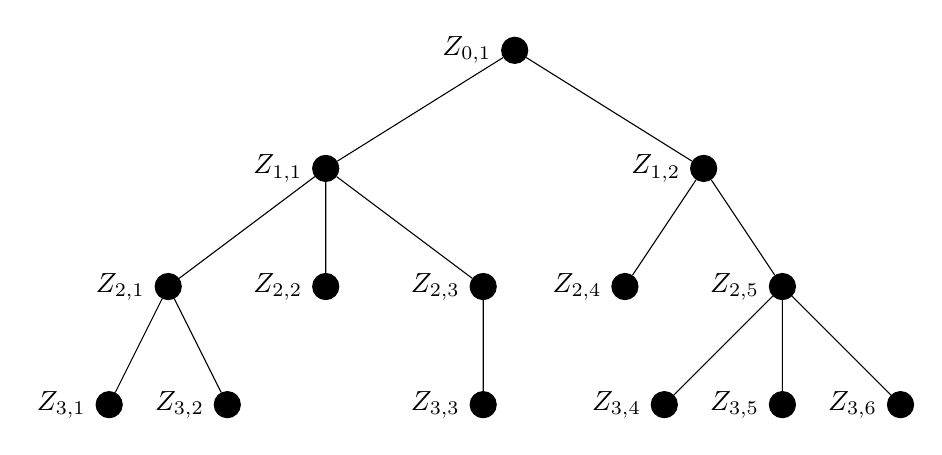
\begin{tikzpicture}[level distance=1.3cm,
        vertex/.style={minimum size=0.5pt,fill,draw,circle},
        level 1/.style={sibling distance=4.8cm, level distance=1.5cm},
        level 2/.style={sibling distance=2cm, level distance=1.5cm},
        level 3/.style={sibling distance=1.5cm, level distance=1.5cm},
        leaf/.style={label={[name=#1]left:$#1$}},
        ]
        \node[vertex, leaf = Z_{0,1}] {}
        child {node[vertex, leaf = Z_{1,1}] {}
            child {node[vertex, leaf = Z_{2,1}] {}
            child {node[vertex, leaf = Z_{3,1}] {}}
            child {node[vertex, leaf = Z_{3,2}] {}}
            }
            child {node[vertex, leaf = Z_{2,2}] {}}
            child {node[vertex, leaf = Z_{2,3}] {}
            child {node[vertex, leaf = Z_{3,3}] {}}
            }
        }
        child {node[vertex, leaf = Z_{1,2}] {}
            child {node[vertex, leaf = Z_{2,4}] {}}
            child {node[vertex, leaf = Z_{2,5}] {}
            child {node[vertex, leaf = Z_{3,4}] {}}
            child {node[vertex, leaf = Z_{3,5}] {}}
            child {node[vertex, leaf = Z_{3,6}] {}}
            }
        };
        \end{tikzpicture}
        \end{center}
    \item $ z $-transform for distribution of $ X_t $:
    \begin{align}
        \Pi_t(s)=\mathbb{E}\left[ s^X_t \right] = \sum_{j=0}^\infty s^j\mathbb{P}\left( X_t=j \right)  \quad L(s)=\mathbb{E}\left[ s^Z \right] =\sum_{j=0}^\infty s^j\mathbb{P}\left( Z=j \right) 
    \end{align}
    and 
    \begin{align}
        \Pi_t(s)=&\sum_{j=0}^\infty \mathbb{E}\left[ s^{X_t}|X_{t-1}=h \right] \mathbb{P}\left( X_{t-1}=j \right) \\
        =&\sum_{j=0}^\infty \left(L(s)\right)^{j}\mathbb{P}\left( X_{t-1}=j \right) \\
        =&\Pi_{t-1}\left(L(s)\right)\\
        (\Pi_1(s)=L(s))=&L^{(t)}(s) 
    \end{align}
    \item Mean and Variance:
    \begin{align}
        \text{Mean}:&\, \mu (t) = \Pi_t'(1)=\mu(0) ^t\\
        \text{Variance}:&\,var(t)=\Pi_t''(1)+\Pi_t'(1)-[\Pi_t'(1)]^2
    \end{align}
    \item Extinction Probability\index{Extinction Probability}
    \begin{align}
        \theta _t=&\mathbb{P}\left( X_t=0 \right)= \sum_{j=0}^\infty \theta ^j_{t-1}\mathbb{P}\left( Z=j \right) \\=
        &L(\theta _{t-1})
    \end{align}
    The eventual extinction is $ \theta ^*=L(\theta ^*) $, the fixed point of $ L(\, \cdot \, ) $.
    There is a phase transformation at $ \mu = 1 $
    \begin{align}
        \mathbb{P}\left( \theta ^*=1 \right) =\begin{cases}
            1,&\mu \leq 1\\
            \text{the first root of }L(\theta )=\theta ,& \mu >1
        \end{cases} 
    \end{align}
    
    Convergence order at phase transition point:
    \begin{align}
        \mathbb{P}\left( X_T>n \right) \sim \begin{cases}
            c_1\mu ^n,&\mu <1\\
            \dfrac{c_2}{n},&\mu =1
        \end{cases}  
    \end{align}
     
\end{itemize}


\subsubsection{Brownian Motion}
\index{Brownian Motion}\index{Wiener Process}\hypertarget{BrownianProcess}{}

Motivation: Brownian motion / Weiner Process $ W_t $\footnote{Symbol $ W_t $ for `Wiener', sometimes uses $ B_t $ for `Brown'.} is similar to a random walk model with $ p=q=1/2 $, but with initial state $ X_0=0 $, and `steps' defined as `a short enough time segmentation'.
\begin{align}
    W_{t=\frac{k}{N}}:= \dfrac{1}{\sqrt{N}} \sum_{i=1}^k \varpi _i,\quad \varpi _i\sim_{\mathrm{i.i.d.} } \mathrm{Unif}\{+1,-1\} 
\end{align}
and have $ N\to \infty $ as a Brownian Motion (Donsker Thm.\index{Donsker Thm.})

Rigorous definition of \textbf{Brownian / Wiener Process}: $ \{W_t:T\geq 0\} $ with $ 0<\sigma ^2<\infty $ is Brownian if
\begin{enumerate}[topsep=2pt,itemsep=2pt]
    \item Starts from $ 0 $: $ \mathbb{P}\left( W_0 \right) =1 $
    \item Independent increment: $ W_{t_1}-W_{s_1}\independent W_{t_2}-W_{s_2} $, $  \forall [t_1,s_1\cap [t_2,s_2]=\emptyset $
    \item Zero mean Normal: $ W_t-W_s\sim N(0,\sigma ^2\vert t-s\vert) $
    \item continuity: $ \mathbb{P}\left( W_t\text{ continuous} \right) =1 $ 
\end{enumerate}

Properties:
\begin{itemize}[topsep=2pt,itemsep=0pt]
        \item Parameters
        \begin{align}
            \begin{cases}
                \text{Mean Function}:\mu (t)=0\\
                \text{Covariance}:\gamma (t,s)=\sigma ^2 \min\{s,t\} 
            \end{cases} 
        \end{align}
        \item m.s. indifferentiable
        \begin{align}
            \mathbb{E}\left[ \left(\dfrac{\partial^{} W_t}{\partial t^{}}\right)^2 \right]\to \infty  
        \end{align}
        which is the reason why the plots for Brownian Motion always looks rugged.
        \item Conditional distribution / Brownian Bridge $ B_t $:
        \begin{align}
            B_t := W_t|W_T=0 \sim N(0,\sigma ^2\dfrac{t(T-t)}{T})
        \end{align}
        \begin{itemize}[topsep=2pt,itemsep=0pt]
            \item Dependent increment: non-zero covariance
        \begin{align}
            \gamma_\mathrm{Bridge}  (t,s) = \sigma ^2\left(\min\{t,s\}-\dfrac{ts}{T}\right)
        \end{align}
            \item Cross definition between Wiener Process and Brownian Bridge:
            \begin{align}
                \begin{cases}
                    B_t:=W_t-\dfrac{t}{T}W_T\\
                    W_t:=B_t+t \sigma ^2 N(0,1) 
                \end{cases}
            \end{align}
            i.e. Brownian Bridge is independent of the terminal of its corresponding Wiener Process $ B_t\independent W_T $.
        \end{itemize}
\end{itemize}

\subsubsection{Poisson Process}\label{SubSubSectionPoissonProcess}
\index{Poisson Process}\hypertarget{PoissonProcess}{}

Motivation: The accumulate events happens at random, with `happening rate' of events as $ \lambda  $
\begin{align}
    N_{t=\frac{k}{N}}:= \sum_{i=1}^k \nu  _i,\quad \nu  _i\sim_{\mathrm{i.i.d.} } \mathrm{Bern}(\dfrac{\lambda }{n}) 
\end{align}

Rigorous Definition of \textbf{Poisson Process}: $ \{N_t:t\geq 0\} $ with rate $ \lambda >0 $ is Poisson if 
\begin{itemize}[topsep=2pt,itemsep=0pt]
    \item Counting Process $ N_t $: $ N_0=0 $, $ N_t\in\mathbb{N} $
    \item Independent Increment: $ N_{t_1}-N_{s_1}\independent N_{t_2}-N_{s_2} $, $ \forall [t_1,s_1\cap [t_2,s_2]=\emptyset $
    \item Poisson increment: $ N_t-N_s\sim P\left(\lambda (t-s)\right) $, $ t\geq s $\footnote{A proof \& another kind of definition concerning the intuition of `rate $ \lambda  $' is here: \url{https://v1ncent19.github.io//texts/Poisson/}.}
\end{itemize}

Properties:
\begin{itemize}[topsep=2pt,itemsep=0pt]
    \item Parameters
    \begin{align}
        \begin{cases}
            \text{Mean Function}:\mu (t)=\lambda t\\
            \text{Covariance}:\gamma (t,s)=\lambda \min\{s,t\} 
        \end{cases}
    \end{align}
    \item Arrival time: $ N_{t_n}=n $ means there are $ n $ events before (and including) $ t_n $, denoted $ \{t_1,t_2,\ldots,t_n\} $. PDF
    \begin{align}
        f_{T_1,T_2,\ldots,T_n}(t_1,t_2,\ldots,t_n)=\lambda ^ne^{-\lambda t_n}\mathbb{I}_{0<t_1<t_2<\ldots<t_n}
    \end{align}
    \item Inter-event time: PDF of time-between-events $ \{u_1,u_2,\ldots,u_n\}:=\{t_1,t_2-t_1,\ldots,t_n-t_{n-1}\} $
    \begin{align}
        f_{U_1,U_2,\ldots,U_n}(u_1,u_2,\ldots,u_n)=\prod_{i=1}^n \lambda e^{-\lambda u_i}\mathbb{I}_{u_i\geq 0}=\sim \otimes{i=1}^n\varepsilon_i (\lambda )
    \end{align}
    
    i.e. time-between-events satisfies exponential distribution
    \begin{align}
        U_i\sim_\mathrm{i.i.d.}  \varepsilon (\lambda ) 
    \end{align}

    \item Conditional distribution
    \begin{align}
        f_{T_1,T_2,\ldots,T_n|N_t=n}(t_1,t_2,\ldots,t_n)=\dfrac{n!}{t^n}\mathbb{I}_{0<t_1<t_2<\ldots<t_n}\sim \mathrm{Unif}\left(\mathbb{I}_{0<t_1<t_2<\ldots<t_n\leq t}\right) 
    \end{align}
    is the PDF of order statistics\footnote{See \autoref{EqaDistributionOfOrderStatistics}.} of i.i.d. $ \mathrm{Unif}(0,t)  $.
    \item Poisson Process and Martingale: 
    \begin{align}
        \tilde{N}_t:=N_t-\lambda t\sim\mathrm{Martingale}  
    \end{align}
    
\end{itemize}


\subsubsection{Birth-Death Process}
\index{Birth-Death Process}
Birth-death process looks like a one-end random-walk with `step' as poisson r.v.(i.e. exponential time-interval) The transition rate \& diagram are:
\begin{center}
    $
    Q=\begin{pNiceMatrix}[first-row,first-col]
        &0&1&2&3&\cdots\,\,\\
        0&-\lambda _0&\lambda _0&&&\\
        1&\mu _1&-\mu _1-\lambda _1&\lambda _1&&\\
        2&&\mu _2&-\mu _2-\lambda _2&\lambda _2&\\
        3&&&\mu _3&\ddots&\ddots\\
        \vdots&&&&\ddots&\ddots
        % \vdots&&&&&1\\
    \end{pNiceMatrix}\qquad \bm{\leftrightharpoons }\qquad
    $
    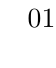
\begin{tikzpicture}[baseline={([yshift = -1ex]current bounding box.center)}]
    \GraphInit[vstyle=Dijkstra]
    \SetGraphUnit{2}
        \tikzset{VertexStyle/.style = {
            shape = rectangle,
            color = black,
            text = black,
            inner sep = 2pt,
            outer sep = 2pt,
            draw}}
        \Vertex[L=$ 0 $]{0}
        \EA[L=$1$](0){1}
        \EA[L=$2$](1){2}
        % \EA[L=$3$](2){3}
        \tikzset{VertexStyle/.style = {
            shape = circle,
            color = white,
            text = black,
            minimum size = 23pt,
            draw}}
        \EA[L=...,unit=1.9 ](2){3}

        \tikzset{EdgeStyle/.style = {->,bend left,thick}}
        \tikzset{LabelStyle/.style = {fill=white}}
        \Edge[label=$ \lambda _0 $](0)(1)
        \Edge[label=$ \lambda _1 $](1)(2)
        \Edge[label=$ \lambda _2 $](2)(3)
        % \Edge[label=$ \lambda _3 $](3)(4)

        \Edge[label=$ \mu _1 $](1)(0)
        \Edge[label=$ \mu _2 $](2)(1)
        \Edge[label=$ \mu _3 $](3)(2)
        % \Edge[label=$ \mu _4 $](4)(3)

    \end{tikzpicture}
    \end{center}

\begin{itemize}[topsep=2pt,itemsep=0pt]
    \item Kolmogorov forward: with a trivial notation that $ \lambda _{-1}=\mu _0=0 $, we have
    \begin{align}
         \dot{p}_i(t)=\lambda _{i-1}p_{i-1}(t)+\mu _{i+1}p_{i+1}(t)-(\lambda _i+\mu _i)p_i(t)
    \end{align}
    \item Stationary Distribution: $ \dot{\pi}^*=0 $ yields 
    \begin{align}
        (\lambda _i+\mu _i)\pi_i^*=\lambda _{i-1}\pi_{i-1}^*+\mu _{i+1}\pi^*_{i+1} 
    \end{align}
    Solution:
    \begin{align}
        \pi^*_i=\begin{cases}
            \dfrac{1}{Z}\dfrac{\lambda _0\lambda _1\ldots\lambda _{i-1}}{\mu _1\mu _2\ldots\mu _i},&i\neq 0\\
            \dfrac{1}{Z},&i=0
        \end{cases},\quad Z=1+\sum_{j=1}^\infty \dfrac{\lambda _0\lambda _1\ldots\lambda _{j-1}}{\mu _1\mu _2\ldots\mu _j}
    \end{align}
    
\end{itemize}








































\subsection{Applications}


\subsubsection{Innovation Sequence}
     
Motivation of Innovation Sequence (新息序列)\index{Innovation Sequence}: construction of linear MMSE $ L(X|Y_1,Y_2,\ldots,Y_n)=L(X|Y) $. Assume that $\mathbb{E}\left[ \vec{Y} \right] =0 $, the prediction is
\begin{align}
    L(X|\vec{Y})=\mathbb{E}\left[ X \right] + cov(X,\vec{Y})var(\vec{Y})^{-1}\vec{Y}
\end{align}
which causes the problem of computation complexity when dimension $ n $ is large. 

Innovation sequence fixed this problem by: instead of projecting on the whole linear combination $ \vec{Y} $ space of size $ (n+1) $, we project on space of each $ Y_i $ sequentially. i.e. define an \textbf{innovation sequence} 
\begin{align}
    \tilde{Y}_1=&Y_1-\mathbb{E}\left[ Y_1 \right] = Y_1 - \mathbb{E}\left[ Y_1 \right] \\
    \tilde{Y}_2=&Y_2-L(Y_2|Y_1) = Y_2-L(Y_2|\tilde{Y}_1)\\
    \tilde{Y}_3=&Y_3-L(Y_3|Y_2Y_1)= Y_3-L(Y_3|\tilde{Y}_2\tilde{Y}_1)\\
    \ldots&\\
    \tilde{Y}_n=&Y_n-L(Y_n|Y_{n-1}\ldots Y_2Y_1)=Y_n-L(Y_n|\tilde{Y}_{n-1}\ldots \tilde{Y}_2\tilde{Y}_1)
\end{align}
where `innovation' means each $ \tilde{Y}_i $ contains the `new information without correlation with previous sequence': $ \mathbb{E}\left[ \tilde{Y_i}\tilde{Y}_j \right]=0\,\forall i\neq j  $. Computation of innovation sequence:
\begin{align}
     \tilde{Y}_k=&Y_k-L(Y_k|\tilde{Y}_{k-1}\ldots \tilde{Y}_1)=Y_k-\mathbb{E}\left[ Y_k \right] -\sum_{j=1}^{k-1}\dfrac{cov(Y_k,\tilde{Y}_{j})}{var(\tilde{Y}_{j})}\tilde{Y}_j,\quad k=1,2,\ldots,n
\end{align}
with a trivial notation that $ Y_{0}=1 $

In this way a linear MMSE $ L(X|\vec{Y}) $ could be written as
\begin{align}
    L(X|\vec{Y})=L(X|\vec{\tilde{Y}})= \mathbb{E}\left[ X \right] +\sum_{i=1}^n \dfrac{cov(X,\tilde{Y}_i)}{var(\tilde{Y}_i)}\tilde{Y}_i=\mathbb{E}\left[ X \right] +\sum_{i=1}^n L\left(X-\mathbb{E}\left[ X \right] |\tilde{Y}_i\right)
\end{align}


I think the idea here is similar to Gram-Schmidt orthogonalization (\autoref{SubSubSectionQRDecomposition}), in which we also construct new components by eliminating projection on previous parts. As a result we have a set of orthogonal elements (here orthogonal means $ \mathbb{E}\left[ \tilde{Y}_i\tilde{Y}_j \right]=0  $ and in Gram-Schmidt means $ q_i'q_j = 0 $, $ i\neq j $). And the result is a `change of basis' of space.




\subsubsection{Markov Decision Processes}
\index{MDPs (Markov Decision Processes)}\index{Episode}\index{Policy}
In decision process/episode, say $ \{(s_t,a_t)\}_{t=0}^T $, we need to determine a \textbf{policy} $ \pi_t $ to take \textbf{action}  $ a_t $ given \textbf{state}  $ s_t $ as
\begin{align}
    a_t\sim \pi_t(\, \cdot \,| s_t) \text{ or simply }a_t=\pi_t(s_t)
\end{align}
then (conditional) \textbf{transition}  probability is a model pre-assumed, say
\begin{align}
    s_{t+1}\sim p_t\left(\, \cdot \, |s_t,a_t\right) 
\end{align}


\begin{point}
    Optimization Target
\end{point}

The optimization target (in each step) is \textbf{reward function} 
\begin{align}
    r_t(s_t,s_{t+1}|a_t)
\end{align}

The `cumulative reward' from step $ t $ is denoted $ \mathcal{V}_{t\leadsto T} $\footnote{In this subsection I usually use the superscript $ \cdot ^{\pi_{t:T}} $ to specify the optimize target.} 
\begin{align}\label{EqaVLearningIteration}
    \mathcal{V}_{t\leadsto T}^{\pi_{t:T}}(s_t)=\mathbb{E}_{s_{t+1}\sim p\left(\, \cdot \, |s_t,a_t=\pi(s_t)\right)}\left[ r_t\left(s_t,s_{t+1}|a_t=\pi_t(s_t)\right)+\gamma \mathcal{V}_{(t+1)\leadsto T}^{\pi_{(t+1):T}} (s_{t+1})\big|s_t\right]
\end{align}
where \textbf{discount factor} $ \gamma<1  $\index{Discount Factor} is induced to focus on recent rewards. By expanding all iteration terms we have
\begin{align}
    \mathcal{V}_{t\leadsto T}^{\pi_{t:T}}(s_t)=&\mathbb{E}_{s_{(t+1):(T+1)}}\left[ \sum_{\tau = t}^T\gamma ^{\tau-t}r_\tau\left(s_\tau,s_{\tau+1}|a_\tau=\pi_\tau(s_\tau)\right)\big|s_t \right]
\end{align}
and the final optimize goal is maximize total reward $ \mathcal{V} $
\begin{align}\label{EqaVLearningTarget}
    \pi_{0:T}^*=&\mathop{\arg\max}\limits_{\pi_{0:T}}\,\mathbb{E}_{s_0\sim p_0(\, \cdot \, )}\left[ \mathcal{V}_{0\leadsto T}^{\pi_{0:T}}(s_0) \right]  \\
    =&\mathop{\arg\max}\limits_{\pi_{0:T}}\,\mathbb{E}_{s_{0:(T+1)}}\left[ \sum_{\tau = 0}^T\gamma ^{\tau}r_\tau\left(s_\tau,s_{\tau+1}|a_\tau=\pi_\tau(s_\tau)\right) \right]
\end{align}



Comments:
\begin{itemize}[topsep=2pt,itemsep=0pt]
    \item The joint distribution of $ s_{t+1,T+1} $ has a complicated dependence on $ p_\tau(\, \cdot \, |s_\tau,a_\tau) $, making the optimization hard to solve directly.
    \item Actually when making decision we should consider a complete process, i.e. $ T\to \infty $, but note that with $ \gamma <1 $, reward at far future is dispensable if rewards are upper-bounded $ r_\tau(s_\tau,s_{\tau+1}|a_\tau)\leq \tilde{r} $, then
    \begin{align}
        \sum_{\tau = T }^\infty\gamma ^{\tau}r_\tau\left(s_\tau,s_{\tau+1}|a_\tau=\pi_\tau(s_\tau)\right) \leq \tilde{r}\dfrac{\gamma ^T}{1-\gamma }
    \end{align}
    which can be bounded below $\varepsilon  \tilde{r} $ for a large enough \textbf{Effective Length}  $ T_\varepsilon  $
    \begin{align}
        \tilde{r}\dfrac{\gamma ^T}{1-\gamma }<\tilde{r}\varepsilon \Rightarrow T_\varepsilon \approx \dfrac{\log[(1-\gamma )\varepsilon ]}{\log \gamma }\sim \mathcal{O}\left( \dfrac{1}{1-\gamma }\log\dfrac{1}{\varepsilon (1-\gamma )} \right)\sim \mathcal{O}(\dfrac{1}{1-\gamma })
    \end{align}
\end{itemize}

\begin{point}
    Algorithm
\end{point}

Solving all $ \pi_{0:T} $ jointly in \autoref{EqaVLearningTarget} is complex. It would be wiser to use the iteration form \autoref{EqaVLearningIteration} and \textit{separate decision making} $ a_t $ \textit{and processing} $ p(\, \cdot \, |s_t,a_t) $. With expected rewards denoted
\begin{align}
    R_t(s_t,a_t)= \mathbb{E}_{s_{t+1}\sim p\left(\, \cdot \, |s_t,a_t\right)}\left[ r_t(s_t,s_{t+1}|a_t)\big| s_t,a_t \right]
\end{align}
total reward $ \mathcal{V}_{t\leadsto T} $ could be written as
\begin{align}
    \mathcal{V}_{t\leadsto T}^{\pi_{t:T}}(s_t)=&\mathbb{E}_{s_{t+1}\sim p\left(\, \cdot \, |s_t,a_t\sim\pi(s_t)\right)}\left[ r_t\left(s_t,s_{t+1}|a_t\sim \pi_t(s_t)\right)+\gamma \mathcal{V}_{(t+1)\leadsto T}^{\pi_{(t+1):T}} (s_{t+1})\Big|s_t\right] \\
    =&{\color{red}\mathbb{E}_{a_t\sim \pi(\, \cdot \, |s_t)}\left[{\color{blue}R_{t}\left(s_t,a_t\right)+  \gamma\mathbb{E}_{s_{t+1}\sim p\left(\, \cdot \, |s_t,a_t\right)}\left[{\color{black}  \mathcal{V}_{(t+1)\leadsto T}^{\pi_{(t+1):T}} (s_{t+1})} \Big| s_t,a_t \right]}  \big|s_t\right]}
\end{align}
with the {red} part as \textbf{State-Value Function}\index{V-Value@$ V $-Value (State-Value Function)}\index{State-Value Function}, or {\color{red}$ V $-value}; the {blue} part as \textbf{Action-Value Function}\index{Action-Value Function}, or {\color{blue}$ Q $-value}
\begin{align}
    {\color{red}V_{t\leadsto T}^{\pi_{t:T}}(s_t)}=&\mathbb{E}_{a_t\sim \pi(\, \cdot \, |s_t)}\left[ Q_{t\leadsto T}^{\pi_{(t+1):T}}(s_t,a_t)  \big|s_t\right]\\
    {\color{blue}Q_{t\leadsto T}^{\pi_{(t+1):T}}(s_t,a_t)}=&R_t\left(s_t,a_t\right)+\gamma \mathbb{E}_{s_{t+1}\sim p\left(\, \cdot \, |s_t,a_t\right)}\left[V_{(t+1)\leadsto T}^{\pi_{(t+1):T}} (s_{t+1})\Big| s_t,a_t\right]
\end{align}

Comments:
\begin{itemize}[topsep=2pt,itemsep=0pt]
    \item The decision process $(s_0,a_0)\leadsto (s_1,a_1)\leadsto\ldots\leadsto (s_T,a_T) $
    is Markovian in $ t=0\to T $ sense, while the reward propagation $ V_{T\leadsto T}\leadsto Q_{(T-1)\leadsto T}\leadsto V_{(T-1)\leadsto T}\leadsto \ldots\leadsto Q_{0\leadsto T}\leadsto V_{0\leadsto T} $ is `Markovian' in $t= T\to 0 $ sense. i.e. solution to optimal $ \pi^* $ obtained by maximizing total reward should go backward.
    \item Duality of optimal $ \{V_{t\leadsto T}^{\pi_{t:T}}\}_{t=0}^T $ ($ V $-learning) and optimal $ \{Q_{t\leadsto T}^{\pi_{t:T}}\}_{t=0}^{T} $ ($ Q $-learning): With $ R_{t}(s_t,a_t) $ actually a given function (for given model $ p(s_{\tau+1}|s_\tau,a_\tau) $),
    \begin{align}
        \begin{cases}
            V_{t\leadsto T}^{\pi_{t:T}}(s_t)={\mathbb{E}_{\color{brown}a_t\sim \pi(\, \cdot \, |s_t)}\left[{R_{t}\left(s_t,a_t\right)+  \gamma\mathbb{E}_{s_{t+1}\sim p\left(\, \cdot \, |s_t,a_t\right)}\left[{\color{black}  V_{(t+1)\leadsto T}^{\pi_{(t+1):T}} (s_{t+1})} \Big| s_t,a_t \right]}  \big|s_t\right]}\\
            Q_{t\leadsto T}^{\pi_{(t+1):T}}(s_t,a_t)=R_t(s_t,a_t)+\gamma \mathbb{E}_{s_{t+1}\sim p\left(\, \cdot \, |s_t,a_t\right)}\left[ \mathbb{E}_{\color{brown}a_{t+1}\sim \pi(\, \cdot \, |s_{t+1})}\left[ Q_{(t+1)\leadsto T}^{\pi_{(t+2):T}}(s_{t+1},a_{t+1})  \big|s_{t+1}\right]  \Big| s_{t+1},a_{t+1}\right]
        \end{cases} 
    \end{align}
    are equivalent, with the same optimization core $ \mathbb{E}_{a_\tau\sim\pi(\, \cdot \, |s_\tau)}\left[ \, \cdot \,  |s_\tau \right]  $. 
    \item[$ \Delta  $] Value function iteration for optimal policy $ \pi^* $:
    \begin{align}
        \pi^*_t(s)=\mathop{\arg\max}\limits_{a} Q_t^*(s,a) ,\quad t=T,T-1,\ldots,0
    \end{align}
    
\end{itemize}
\begin{algorithm}{Value Iteration}
        \begin{enumerate}[topsep=2pt,itemsep=2pt]
            \item $ V^*_{T+1}\equiv 0 $
            \item \textit{for} $ t=T,T-1,\ldots,1 $
            \begin{enumerate}[topsep=2pt,itemsep=2pt]
                \item $ Q $-expectation step:
                \begin{align}
                  Q^*_t(s,a)=R_t(s,a)+\gamma \mathbb{E}_{\tilde{s}\sim p(\, \cdot \, |s,a)}\left[ V^*_{t+1}(\tilde{s}) \big|s,a\right]    
                \end{align}
                \item $ V $-Optimal step:
                \begin{align}
                     \begin{cases}\label{EqaValueIterationProcess}
                        \pi^*_t(s)=&\mathop{\arg\max}\limits_{a}Q_t^*(s,a)\\
                        V^*_t(s)= & \mathop{\max}\limits_{a} Q^*_t(s,a)=Q^*_{t}(s,\pi^*_t(s)) 
                     \end{cases}
                \end{align}
            \end{enumerate}
            i.e. a $ (Q_t,V_t) $ `backward propagation'.
        \end{enumerate}
    \end{algorithm}

\begin{point}
    $ Q $-Learning\index{Q-Learning@$ Q $-Learning}
\end{point}

Motivation: for some more complex cases, e.g.
\begin{itemize}[topsep=2pt,itemsep=0pt]
    \item The functional form of reward $ r_t(s_t,s_{t+1}|a_t) $ or $ R_{t}(s_t,a_t) $ is unknown
    \item The transition probability $ s_{t+1}\sim p(\, \cdot \, |s_t,a_t) $ is unknown
    \item The phase space is too large to compute point wise
\end{itemize}
Note that the above optimize process \autoref{EqaValueIterationProcess} is an optimization w.r.t. $ Q_t(\, \cdot \, ,\, \cdot \, ) $, we can first learn the functional form of $ Q(\, \cdot \, ,\, \cdot \, ) $ (or its function approximation), and thus get the policy $ \pi^* $. The $ Q $-learning process can have the following form:
\begin{align}
    \hat{Q}^{(\tau+1)}(s_{t},a_{t})\leftarrow \overbrace {\hat{Q}^{(\tau)}(s_{t},a_{t})}^{\text{current value}}+\alpha \cdot \overbrace{\bigg(\underbrace {R_t(s_t,a_t)+\gamma \cdot \underbrace {\max _{a}\hat{Q}^{(\tau)}(s_{t+1},a)} _{\text{estimate of optimal future value}}} _{\text{new value (temporal difference target)}}-\underbrace {\hat{Q}^{(\tau)}(s_{t},a_{t})} _{\text{current value}}\bigg )} ^{\text{temporal difference}}
\end{align}
with some known \textit{final/terminal} state $ \{s_\mathrm{final} \} $, where $ Q(s_\mathrm{final},a )\equiv 0,\,\forall a $


\begin{algorithm}{$ Q $-Learning}
\begin{enumerate}[topsep=2pt,itemsep=2pt]
    \item Initialize a tentative $ Q^{(0)}_{t}(\, \cdot \, ,\, \cdot \, ) $, say $ Q\equiv 0 $
    \item \textit{for} $ \tau=0,1,2,\ldots $ \textit{until} $ Q(\, \cdot \, ,\, \cdot \, ) $ converge:
    \begin{enumerate}[topsep=2pt,itemsep=2pt]
        \item Initialize some $ s_1 $
        \item \textit{for} $ t=1,2,\ldots $ \textit{until} $ s_{t}\in\{s_\mathrm{final} \} $: optimize the function form (approximation) $ Q(\, \cdot \, ,\, \cdot \, ) $
        \begin{align}
            \hat{Q}^{(\tau+1)}(s_t,a_t)\leftarrow& \hat{Q}^{(\tau)}(s_t,a_t)+\alpha \left(R_t(s_t,a_t)+\gamma \mathop{\max}\limits_{a}\hat{Q}^{(\tau)}_{t+1}(s_{t+1},a)-\hat{Q}^{(\tau)}_t(s_t,a_t) \right)\\
            s_{t+1}\leftarrow& p_t(s_t,a_t)
        \end{align}
    \end{enumerate}
\end{enumerate}
\end{algorithm}
    



% $ \lim_{u\to\infty}C_X(u)=0 \Rightarrow \forall \varepsilon >0,\,\exists u_\varepsilon $ s.t. $ C_X(u_\varepsilon )<\varepsilon  $, then for $ T $ large enough
% \begin{align}
%     \dfrac{2}{T}\int_{0}^T(1-\dfrac{\tau}{T})C_X(\tau)\,\mathrm{d}\tau =&\dfrac{2}{T}\left[\int_{0}^{u_\varepsilon }(1-\dfrac{\tau}{T})C_X(\tau)\,\mathrm{d}\tau + \int_{u_\varepsilon }^T(1-\dfrac{\tau}{T})C_X(\tau)\,\mathrm{d}\tau\right]\\
%     \leq&\dfrac{2}{T} \int_{0}^{u_\varepsilon }C_X(0)\,\mathrm{d}\tau +\dfrac{2}{T} \int_{0 }^T (1-\dfrac{\tau}{T})\varepsilon \,\mathrm{d}\tau  \\
%     =&\dfrac{2u_\varepsilon C_X(0)}{T}+\varepsilon \leq (2C_X(0)+1)\varepsilon 
% \end{align}



% General definition of Ergodicity: for any given $ \{t_1,t_2,\ldots,t_m\} $
% \begin{align}
%     \lim_{T\to\infty}\int_{0}^\infty f(X_{t_1+\tau},X_{t_2+\tau},\ldots,X_{t_m+\tau})\,\mathrm{d}\tau = \mathbb{E}\left[ f(X_{t_1},X_{t_2},\ldots,X_{t_m}) \right]  
% \end{align}

% e.g. stationary Gaussian with $ \mathrm{Cross}_X(\tau)\to 0   $ is ergodic in m.s. and a.s. sense.


\subsubsection{Karhunen-Loève Expansion}

Karhunen-Loève Expansion (KL Expansion)\index{KL Expansion (Karhunen-Loève Expansion)} is a coutinuous version of PCA \autoref{EqaCurseOfDimensionality}. The idea is a decomposition 
\begin{align}
    X(t)=\sum_{i}X_i\phi _i(t) 
\end{align}
i.e. we add an extra step in mapping
\begin{align}
    X(\, \cdot \, ):\, \Omega\mapsto \{X_i\}\mapsto \mathcal{T}\times \mathbb{R}  
\end{align}
a special set of $ \{X_i,\phi_i\} $ is given by KL expansion.

\begin{point}
    Derivations
\end{point}

First note that $ R(s,t):=\mathbb{E}\left[ X(s)X(t) \right] $ is a Kernel (see \autoref{EqaKernelFunction}), with positive semi-definition and symmetry. Then by Mercer's Thm., it has eigen-function decomposition
\begin{align}
    R(s,t) =\sum_{i} \lambda _i\phi _i(s)\phi _i(t) \Leftrightarrow \langle R(s,\, \cdot \, ),\phi_i\rangle = \lambda _i\phi_i(s)
\end{align}
where eigen functions are orthonormal
\begin{align}
    \langle \phi _i, \phi _j \rangle := \int_\tau \phi _i(\tau)\phi _j(\tau)\,\mathrm{d}\tau = \delta _{ij}
\end{align}

using $ \{\phi _i\} $ as function basis, KL coefficients are r.v. 
\begin{align}
    X_i=\langle X_t, \phi _i\rangle  
\end{align}
with
\begin{align}
    \mathbb{E}\left[ X_iX_j \right] = \langle \phi_i | X_t\rangle \langle X_t| \phi_j\rangle =  \langle \phi_i | R(s,t) | \phi_j\rangle = \delta _{ij}\lambda _i
\end{align}

\begin{point}
Other Concepts
\end{point}
\begin{itemize}[topsep=2pt,itemsep=0pt]
    \item Total energy:
    \begin{align}
        E=\mathbb{E}\left[ \left\langle X_t,X_t \right\rangle \right]=\sum_i\lambda _i
    \end{align}
    \item Rank: $ \mathrm{rank}\left(\{\mathbb{E}\left[ X_iX_j \right] \}\right) = \#(\lambda _i\neq 0) $ is also the rank of the process.
    
\end{itemize}

    














\subsubsection{Kalman Filter}
\begin{point}
    Model
\end{point}

    \textbf{Kalman Filter}\index{Kalman Filter} is an auto-regressive / iterative filter for estimating the \textbf{state} $ x_t $ from \textbf{observable}\footnote{Here I prefer the name as in Quantum mechanics `Observable'.} $ z_t $. The model structure, as in \autoref{FigKalmanStructure}, is a Hidden Markov Model (HMM)\index{HMM (Hidden Markov Model)} with linear operator.
    \begin{align}
        \text{State: }&x_{k}=F_{k}x_{k-1}+w_{k} \\
        \text{Observable: }&z_{k}=H_kx_k+v_k
    \end{align}  
    where $ w_k,\,v_k $ is noise / random error, usually with (multivariate) Normal distribution
    \begin{align}
        w_k\sim N(0,Q_k),\qquad v_k\sim N(0,R_k) 
    \end{align}
    the initial state denoted
    \begin{align}
        x_0\sim N(\hat{x}_{0|0}, P _{0|0}) 
    \end{align}

\begin{figure}[H]
    \centering
    

\tikzset{every picture/.style={line width=0.75pt}} %set default line width to 0.75pt        

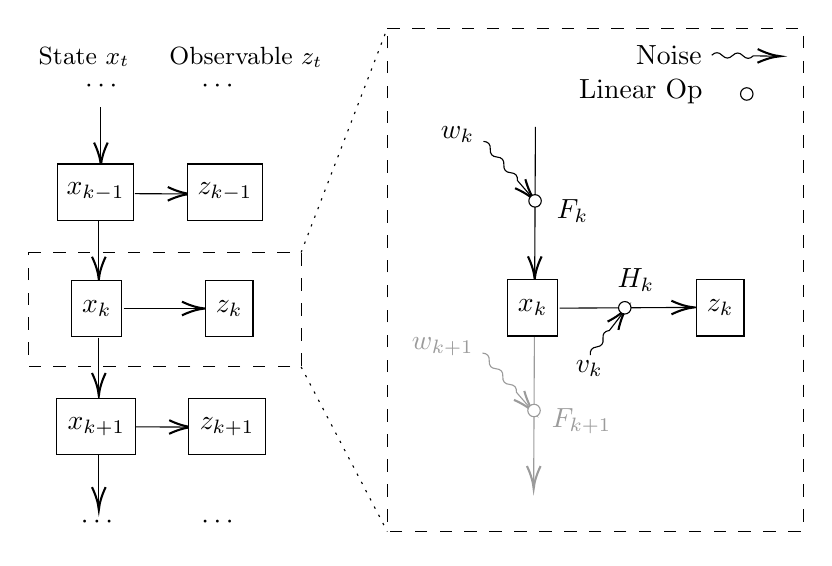
\begin{tikzpicture}[x=0.75pt,y=0.75pt,yscale=-1,xscale=1]
%uncomment if require: \path (0,300); %set diagram left start at 0, and has height of 300

%Straight Lines [id:da8051072890440967] 
\draw [color={rgb, 255:red, 0; green, 0; blue, 0 }  ,draw opacity=1 ][fill={rgb, 255:red, 255; green, 255; blue, 255 }  ,fill opacity=1 ]   (251.33,83.49) .. controls (253.68,83.66) and (254.78,84.92) .. (254.61,87.27) .. controls (254.44,89.62) and (255.53,90.88) .. (257.88,91.05) .. controls (260.23,91.22) and (261.33,92.48) .. (261.16,94.83) .. controls (260.99,97.18) and (262.08,98.43) .. (264.43,98.6) .. controls (266.78,98.77) and (267.88,100.03) .. (267.71,102.38) -- (269.64,104.61) -- (274.88,110.66) ;
\draw [shift={(276.19,112.17)}, rotate = 229.09] [color={rgb, 255:red, 0; green, 0; blue, 0 }  ,draw opacity=1 ][line width=0.75]    (10.93,-3.29) .. controls (6.95,-1.4) and (3.31,-0.3) .. (0,0) .. controls (3.31,0.3) and (6.95,1.4) .. (10.93,3.29)   ;
%Straight Lines [id:da8443065915101042] 
\draw    (66.01,122.03) -- (66.01,148.03) ;
\draw [shift={(66.01,150.03)}, rotate = 270] [color={rgb, 255:red, 0; green, 0; blue, 0 }  ][line width=0.75]    (10.93,-3.29) .. controls (6.95,-1.4) and (3.31,-0.3) .. (0,0) .. controls (3.31,0.3) and (6.95,1.4) .. (10.93,3.29)   ;
%Straight Lines [id:da6875878363586321] 
\draw    (66.01,178.03) -- (66.01,204.03) ;
\draw [shift={(66.01,206.03)}, rotate = 270] [color={rgb, 255:red, 0; green, 0; blue, 0 }  ][line width=0.75]    (10.93,-3.29) .. controls (6.95,-1.4) and (3.31,-0.3) .. (0,0) .. controls (3.31,0.3) and (6.95,1.4) .. (10.93,3.29)   ;
%Straight Lines [id:da05843745637022657] 
\draw    (78.01,164.03) -- (115.01,164.03) ;
\draw [shift={(117.01,164.03)}, rotate = 180] [color={rgb, 255:red, 0; green, 0; blue, 0 }  ][line width=0.75]    (10.93,-3.29) .. controls (6.95,-1.4) and (3.31,-0.3) .. (0,0) .. controls (3.31,0.3) and (6.95,1.4) .. (10.93,3.29)   ;
%Straight Lines [id:da11088548439510282] 
\draw    (67.01,67.03) -- (67.01,93.03) ;
\draw [shift={(67.01,95.03)}, rotate = 270] [color={rgb, 255:red, 0; green, 0; blue, 0 }  ][line width=0.75]    (10.93,-3.29) .. controls (6.95,-1.4) and (3.31,-0.3) .. (0,0) .. controls (3.31,0.3) and (6.95,1.4) .. (10.93,3.29)   ;
%Straight Lines [id:da19051414013865076] 
\draw    (66.01,233.03) -- (66.01,259.03) ;
\draw [shift={(66.01,261.03)}, rotate = 270] [color={rgb, 255:red, 0; green, 0; blue, 0 }  ][line width=0.75]    (10.93,-3.29) .. controls (6.95,-1.4) and (3.31,-0.3) .. (0,0) .. controls (3.31,0.3) and (6.95,1.4) .. (10.93,3.29)   ;
%Straight Lines [id:da7993986672570081] 
\draw    (83.34,108.7) -- (108.16,108.82) ;
\draw [shift={(110.16,108.83)}, rotate = 180.29] [color={rgb, 255:red, 0; green, 0; blue, 0 }  ][line width=0.75]    (10.93,-3.29) .. controls (6.95,-1.4) and (3.31,-0.3) .. (0,0) .. controls (3.31,0.3) and (6.95,1.4) .. (10.93,3.29)   ;
%Straight Lines [id:da6382436414377908] 
\draw    (84.01,221.03) -- (108.83,221.16) ;
\draw [shift={(110.83,221.17)}, rotate = 180.29] [color={rgb, 255:red, 0; green, 0; blue, 0 }  ][line width=0.75]    (10.93,-3.29) .. controls (6.95,-1.4) and (3.31,-0.3) .. (0,0) .. controls (3.31,0.3) and (6.95,1.4) .. (10.93,3.29)   ;
%Rounded Rect [id:dp614251386292366] 
\draw  [dash pattern={on 4.5pt off 4.5pt}] (32,137) .. controls (32,137) and (32,137) .. (32,137) -- (163.49,137) .. controls (163.49,137) and (163.49,137) .. (163.49,137) -- (163.49,192.17) .. controls (163.49,192.17) and (163.49,192.17) .. (163.49,192.17) -- (32,192.17) .. controls (32,192.17) and (32,192.17) .. (32,192.17) -- cycle ;
%Straight Lines [id:da642038681386998] 
\draw [color={rgb, 255:red, 0; green, 0; blue, 0 }  ,draw opacity=1 ][fill={rgb, 255:red, 255; green, 255; blue, 255 }  ,fill opacity=1 ]   (276.37,76.48) -- (276.02,147.86) ;
\draw [shift={(276.01,149.86)}, rotate = 270.28] [color={rgb, 255:red, 0; green, 0; blue, 0 }  ,draw opacity=1 ][line width=0.75]    (10.93,-3.29) .. controls (6.95,-1.4) and (3.31,-0.3) .. (0,0) .. controls (3.31,0.3) and (6.95,1.4) .. (10.93,3.29)   ;
%Straight Lines [id:da3676361709618625] 
\draw    (288.01,163.86) -- (350.83,163.5) ;
\draw [shift={(352.83,163.49)}, rotate = 179.67] [color={rgb, 255:red, 0; green, 0; blue, 0 }  ][line width=0.75]    (10.93,-3.29) .. controls (6.95,-1.4) and (3.31,-0.3) .. (0,0) .. controls (3.31,0.3) and (6.95,1.4) .. (10.93,3.29)   ;
%Straight Lines [id:da8799353629961175] 
\draw    (302.83,186.49) .. controls (302.53,184.15) and (303.55,182.83) .. (305.89,182.53) .. controls (308.23,182.23) and (309.25,180.91) .. (308.94,178.57) .. controls (308.63,176.23) and (309.65,174.91) .. (311.99,174.61) -- (314.32,171.6) -- (319.2,165.26) ;
\draw [shift={(320.42,163.68)}, rotate = 127.63] [color={rgb, 255:red, 0; green, 0; blue, 0 }  ][line width=0.75]    (10.93,-3.29) .. controls (6.95,-1.4) and (3.31,-0.3) .. (0,0) .. controls (3.31,0.3) and (6.95,1.4) .. (10.93,3.29)   ;
%Straight Lines [id:da3845121992781433] 
\draw [color={rgb, 255:red, 155; green, 155; blue, 155 }  ,draw opacity=1 ]   (275.87,177.48) -- (275.52,248.86) ;
\draw [shift={(275.51,250.86)}, rotate = 270.28] [color={rgb, 255:red, 155; green, 155; blue, 155 }  ,draw opacity=1 ][line width=0.75]    (10.93,-3.29) .. controls (6.95,-1.4) and (3.31,-0.3) .. (0,0) .. controls (3.31,0.3) and (6.95,1.4) .. (10.93,3.29)   ;
%Straight Lines [id:da9798416569763584] 
\draw [color={rgb, 255:red, 155; green, 155; blue, 155 }  ,draw opacity=1 ]   (250.83,185.49) .. controls (253.18,185.66) and (254.28,186.92) .. (254.11,189.27) .. controls (253.94,191.62) and (255.03,192.88) .. (257.38,193.05) .. controls (259.73,193.22) and (260.83,194.48) .. (260.66,196.83) .. controls (260.49,199.18) and (261.58,200.43) .. (263.93,200.6) .. controls (266.28,200.77) and (267.38,202.03) .. (267.21,204.38) -- (269.14,206.61) -- (274.38,212.66) ;
\draw [shift={(275.69,214.17)}, rotate = 229.09] [color={rgb, 255:red, 155; green, 155; blue, 155 }  ,draw opacity=1 ][line width=0.75]    (10.93,-3.29) .. controls (6.95,-1.4) and (3.31,-0.3) .. (0,0) .. controls (3.31,0.3) and (6.95,1.4) .. (10.93,3.29)   ;
%Rounded Rect [id:dp9419817408683995] 
\draw  [dash pattern={on 4.5pt off 4.5pt}] (205,28.99) .. controls (205,28.99) and (205,28.99) .. (205,28.99) -- (405.33,28.99) .. controls (405.33,28.99) and (405.33,28.99) .. (405.33,28.99) -- (405.33,271.49) .. controls (405.33,271.49) and (405.33,271.49) .. (405.33,271.49) -- (205,271.49) .. controls (205,271.49) and (205,271.49) .. (205,271.49) -- cycle ;
%Straight Lines [id:da916303967111838] 
\draw  [dash pattern={on 0.84pt off 2.51pt}]  (163.49,137) -- (205,28.99) ;
%Straight Lines [id:da8876073772934547] 
\draw  [dash pattern={on 0.84pt off 2.51pt}]  (163.49,192.17) -- (205,271.49) ;
%Shape: Circle [id:dp27142797833084686] 
\draw  [color={rgb, 255:red, 0; green, 0; blue, 0 }  ,draw opacity=1 ][fill={rgb, 255:red, 255; green, 255; blue, 255 }  ,fill opacity=1 ] (273.19,112.17) .. controls (273.19,110.51) and (274.53,109.17) .. (276.19,109.17) .. controls (277.85,109.17) and (279.19,110.51) .. (279.19,112.17) .. controls (279.19,113.83) and (277.85,115.17) .. (276.19,115.17) .. controls (274.53,115.17) and (273.19,113.83) .. (273.19,112.17) -- cycle ;
%Shape: Circle [id:dp746836452749982] 
\draw  [fill={rgb, 255:red, 255; green, 255; blue, 255 }  ,fill opacity=1 ] (316.42,163.68) .. controls (316.42,162.02) and (317.76,160.68) .. (319.42,160.68) .. controls (321.08,160.68) and (322.42,162.02) .. (322.42,163.68) .. controls (322.42,165.33) and (321.08,166.68) .. (319.42,166.68) .. controls (317.76,166.68) and (316.42,165.33) .. (316.42,163.68) -- cycle ;
%Shape: Circle [id:dp7897054395526044] 
\draw  [color={rgb, 255:red, 155; green, 155; blue, 155 }  ,draw opacity=1 ][fill={rgb, 255:red, 255; green, 255; blue, 255 }  ,fill opacity=1 ] (272.69,213.17) .. controls (272.69,211.51) and (274.03,210.17) .. (275.69,210.17) .. controls (277.35,210.17) and (278.69,211.51) .. (278.69,213.17) .. controls (278.69,214.83) and (277.35,216.17) .. (275.69,216.17) .. controls (274.03,216.17) and (272.69,214.83) .. (272.69,213.17) -- cycle ;
%Straight Lines [id:da11141445571255759] 
\draw    (361.33,41.99) .. controls (363.02,40.35) and (364.69,40.38) .. (366.33,42.07) .. controls (367.98,43.76) and (369.64,43.78) .. (371.33,42.14) .. controls (373.02,40.5) and (374.69,40.53) .. (376.33,42.22) .. controls (377.98,43.91) and (379.64,43.93) .. (381.33,42.29) -- (384.33,42.34) -- (392.33,42.46) ;
\draw [shift={(394.33,42.49)}, rotate = 180.87] [color={rgb, 255:red, 0; green, 0; blue, 0 }  ][line width=0.75]    (10.93,-3.29) .. controls (6.95,-1.4) and (3.31,-0.3) .. (0,0) .. controls (3.31,0.3) and (6.95,1.4) .. (10.93,3.29)   ;
%Shape: Circle [id:dp11478084942637645] 
\draw  [fill={rgb, 255:red, 255; green, 255; blue, 255 }  ,fill opacity=1 ] (375.19,60.67) .. controls (375.19,59.01) and (376.53,57.67) .. (378.19,57.67) .. controls (379.85,57.67) and (381.19,59.01) .. (381.19,60.67) .. controls (381.19,62.33) and (379.85,63.67) .. (378.19,63.67) .. controls (376.53,63.67) and (375.19,62.33) .. (375.19,60.67) -- cycle ;

% Text Node
\draw  [fill={rgb, 255:red, 255; green, 255; blue, 255 }  ,fill opacity=1 ]  (45.93,94.42) -- (82.93,94.42) -- (82.93,121.42) -- (45.93,121.42) -- cycle  ;
\draw (64.43,107.92) node    {$x_{k-1}$};
% Text Node
\draw  [fill={rgb, 255:red, 255; green, 255; blue, 255 }  ,fill opacity=1 ]  (53.04,150.42) -- (77.04,150.42) -- (77.04,177.42) -- (53.04,177.42) -- cycle  ;
\draw (65.04,163.92) node    {$x_{k}$};
% Text Node
\draw  [fill={rgb, 255:red, 255; green, 255; blue, 255 }  ,fill opacity=1 ]  (45.81,207.42) -- (83.81,207.42) -- (83.81,234.42) -- (45.81,234.42) -- cycle  ;
\draw (64.81,220.92) node    {$x_{k+1}$};
% Text Node
\draw  [fill={rgb, 255:red, 255; green, 255; blue, 255 }  ,fill opacity=1 ]  (108.77,94.42) -- (144.77,94.42) -- (144.77,121.42) -- (108.77,121.42) -- cycle  ;
\draw (126.77,107.92) node    {$z_{k-1}$};
% Text Node
\draw  [fill={rgb, 255:red, 255; green, 255; blue, 255 }  ,fill opacity=1 ]  (117.31,150.42) -- (140.31,150.42) -- (140.31,177.42) -- (117.31,177.42) -- cycle  ;
\draw (128.81,163.92) node    {$z_{k}$};
% Text Node
\draw  [fill={rgb, 255:red, 255; green, 255; blue, 255 }  ,fill opacity=1 ]  (109.31,207.42) -- (146.31,207.42) -- (146.31,234.42) -- (109.31,234.42) -- cycle  ;
\draw (127.81,220.92) node    {$z_{k+1}$};
% Text Node
\draw (68.26,57.2) node    {$\cdots $};
% Text Node
\draw (66.26,267.2) node    {$\cdots $};
% Text Node
\draw (58.87,42.86) node  [font=\small] [align=left] {State$\displaystyle \ x_{t}$};
% Text Node
\draw (136.88,42.86) node  [font=\small] [align=left] {Observable$\displaystyle \ z_{t}$};
% Text Node
\draw (124.26,56.86) node    {$\cdots $};
% Text Node
\draw (124.26,267.2) node    {$\cdots $};
% Text Node
\draw  [color={rgb, 255:red, 0; green, 0; blue, 0 }  ,draw opacity=1 ][fill={rgb, 255:red, 255; green, 255; blue, 255 }  ,fill opacity=1 ]  (263.04,150.25) -- (287.04,150.25) -- (287.04,177.25) -- (263.04,177.25) -- cycle  ;
\draw (275.04,163.75) node    {$x_{k}$};
% Text Node
\draw  [fill={rgb, 255:red, 255; green, 255; blue, 255 }  ,fill opacity=1 ]  (353.87,150.25) -- (376.87,150.25) -- (376.87,177.25) -- (353.87,177.25) -- cycle  ;
\draw (365.37,163.75) node    {$z_{k}$};
% Text Node
\draw (238.82,80.26) node  [color={rgb, 255:red, 0; green, 0; blue, 0 }  ,opacity=1 ]  {$w_{k}$};
% Text Node
\draw (302.31,192.76) node    {$v_{k}$};
% Text Node
\draw (231.7,182.26) node  [color={rgb, 255:red, 155; green, 155; blue, 155 }  ,opacity=1 ]  {$w_{k+1}$};
% Text Node
\draw (294.24,117.24) node  [color={rgb, 255:red, 0; green, 0; blue, 0 }  ,opacity=1 ]  {$F_{k}$};
% Text Node
\draw (298.62,218.24) node  [color={rgb, 255:red, 155; green, 155; blue, 155 }  ,opacity=1 ]  {$F_{k+1}$};
% Text Node
\draw (324.74,150.24) node    {$H_{k}$};
% Text Node
\draw (357.69,41.99) node [anchor=east] [inner sep=0.75pt]   [align=left] {Noise};
% Text Node
\draw (358.19,59.49) node [anchor=east] [inner sep=0.75pt]   [align=left] {Linear Op};


\end{tikzpicture}
\caption{HMM structure of Kalman Filter}
\label{FigKalmanStructure}
\end{figure}

\begin{point}
    Algorithm
\end{point}

Motivation: what we could observe is $ \{z_k\} $ sequence, with pre-specified $ \{F_k,H_k,Q_k,R_k\} $, which are part of the model. We hope to (linearly) estimate the value and variance of the hidden state $ x_k $
\begin{align}
    \text{value: }&\hat{x}_{k|k-1}:=L(x_k|z_1\ldots z_{k-1})\\
    \text{variance: }&P_{k|k-1}:=var\left(x_k-\hat{x}_{k|k-1}\right)
\end{align}

\begin{algorithm}{Kalman Filter}
    \begin{enumerate}[topsep=2pt,itemsep=2pt]
        \item Initial State: $ x_0\sim N(\hat{x}_{0|0}, P _{0|0})  $; Model given $ \{F_k,H_k,Q_k,R_k\} $;
        \item \textit{for} $ k=1,2,\ldots $
        \begin{enumerate}[topsep=2pt,itemsep=2pt]
            \item State Predict: $ \, \cdot \, _{k-1|k-1}\mapsto \, \cdot \, _{k|k-1} $
            \begin{align}
                \text{prior state: }&\hat{x}_{k|k-1}=F_k \hat{x}_{k-1|k-1}\\
                \text{prior cov: }&P_{k|k-1}=F_kP_{k-1|k-1}F_k'+Q_k
            \end{align}
            \item Information Update: weighting btw. $ \, \cdot \, _{k|k-1} $ and $ \, \cdot \, _{k} $\index{Optimal Kalman Gain}
            \begin{align}
                \text{innovation seq: }&\tilde{z}_k=z_k-H_k\hat{x}_{k|k-1}\\
                \text{innovation cov: }&S_k=H_kP_{k|k-1}H_k'+R_k\\
                \text{(Optimal) Kalman gain: }&K_k=P_{k|k-1}H_k'S_k^{-1}\\
                &{\color{white}K_k}=P_{k|k-1}H_k'\left(H_kP_{k|k-1}H_k'+R_k\right)^{-1}
            \end{align}
            \item State Update: $ \, \cdot \, _{k|k-1}\mapsto \, \cdot \, _{k|k} $
            \begin{align}
                \text{posterior state: }&\hat{x}_{k|k}=\hat{x}_{k|k-1}+K_k\tilde{z}_k\\
                &{\color{white}\hat{x}_{k|k}}=\hat{x}_{k|k-1}+K_k\left(z_k-H_k\hat{x}_{k|k-1}\right)\\
                &{\color{white}\hat{x}_{k|k}}=\left(I-K_kH_k\right)\hat{x}_{k|k-1}+K_kz_k\\
                \text{posterior cov: }&P_{k|k}=\left(I-K_kH_k\right)P_{k|k-1}\left(I-K_kH_k\right)'+K_kR_kK_k'\\
                &{\color{white}P_{k|k}}=\left(I-K_kH_k\right)P_{k|k-1}
            \end{align}
        \end{enumerate}
    \end{enumerate}
\end{algorithm}
    

\begin{point}
    Derivation Details
\end{point}

\begin{itemize}[topsep=2pt,itemsep=0pt]
    \item Key concepts in Kalman Filter:
    \begin{align}
        \text{prior state: }&\hat{x}_{k|k-1}=L(x_k|z_1\ldots z_{k-1}) \\
        \text{prior covariance: }&P_{k|k-1}=var\left(x_k-\hat{x}_{k|k-1}\right)\\
        \text{posterior state: }&\hat{x}_{k|k}=L(x_k|z_1\ldots z_{k}) \\
        \text{posterior covariance: }&P_{k|k}=var\left(x_k-\hat{x}_{k|k}\right)\\
        \text{Kalman gain: }&K_k
    \end{align}
    \item[(a1)] prior state prediction
    \begin{align}
        \hat{x}_{k|k-1}=&L(x_k|z_1\ldots z_{k-1})=L(F_kx_{k-1}+w_k|z_1\ldots z_{k-1})=F_k\hat{x}_{k-1|k-1} 
    \end{align}
    \item[(a2)] prior covariance prediction
    \begin{align}
         P_{k|k-1}=&var\left(x_{k}-\hat{x}_{k|k-1}\right)=var\left(F_k(x_{k-1}-\hat{x}_{k-1|k-1})+w_k\right)=F_kP_{k-1|k-1}F_k'+Q_k
    \end{align}
    \item[(b1)] innovation sequence of $ z_k $
    \begin{align}
        \tilde{z}_k=z_k-L(z_k|z_1\ldots z_{k-1})=z_k-L(H_kx_k+v_k|z_1\ldots z_{k-1} )=z_k-H_k\hat{x}_{k|k-1}
    \end{align}
    \item[(b2)] innovation sequence variance
    \begin{align}
        S_k:=var(\tilde{z}_k)=&var\left( z_k-H_k\hat{x}_{k|k-1} \right)=var\left(H_k(x_k-\hat{x}_{k|k-1})+v_k\right)=H_kP_{k|k-1}H_k'+R_k
    \end{align}
    \item[(b3)] Optimal Kalman gain is obtained by
    \begin{align}
        \hat{x}_{k|k}=\hat{x}_{k|k-1}+L(x_k-\mathbb{E}\left[ x \right]|\tilde{z}_k )=\hat{x}_{k|k-1}+cov(x_k,\tilde{z}_k)var(\tilde{z}_k)^{-1}\tilde{z}_k :=\hat{x}_{k|k-1}+K_k\tilde{z}_k
    \end{align}
    i.e. Optimal Kalman gain in the combination coefficient in MMSE.
    \begin{align}
        K_k=& cov(x_k,\tilde{z}_k)var(\tilde{z}_k)^{-1}=cov(x_k,H_k(x_k-\hat{x}_{k|k-1})+v_k)S_k^{-1}\\
        =&cov(x_k-\hat{x}_{k|k-1},x_k-\hat{x}_{k|k-1})H_k'S_k^{-1}\\
        =&P_{k|k-1}H_k'S_k^{-1}
    \end{align}
    here we use the property of MMSE
    \begin{align}
        cov(\hat{x}_{k|k-1},x_k-\hat{x}_{k|k-1})=0 
    \end{align}
    
    
    \item[(c1)] posterior state update
    \begin{align}\label{EqaKalmanPosteriorUpdate}
        \hat{x}_{k|k}=\hat{x}_{k|k-1}+K_k\tilde{z}_k=\left(I-K_kH_k\right)\hat{x}_{k|k-1}+K_kz_k
    \end{align}
    \item[(c2)] posterior variance update
    \begin{align}\label{EqaKalmanFilterPostVarUpdate}
        P_{k|k}=&var(x_k-\hat{x}_{k|k})=var\left( x_k-\hat{x}_{k|k-1}-K_k(z_k-H_k\hat{x}_{k|k-1}) \right)\\
        =&var\left( x_k-\hat{x}_{k|k-1}-K_k(H_kx_k+v_k-H_k\hat{x}_{k|k-1}) \right)\\
        =&var\left((I-K_kH_k)(x_k-\hat{x}_{k|k-1})-K_kv_k\right)\\
        =&(I-K_kH_k)P_{k|k-1}(I-K_kH_k)'+K_kR_kK_k'
    \end{align}
    further if $ K_k $ takes optimal Kalman gain, 
    \begin{align}
        \color{brown}K_kS_kK_k'= P_{k|k-1}H_k'K_k'
    \end{align}
    
    we have a simplification
    \begin{align}
        P_{k|k}=& (I-K_kH_k)P_{k|k-1}(I-K_kH_k)'+K_kR_kK_k' \\
        =& P_{k|k-1}-K_kH_kP_{k|k-1}-P_{k|k-1}H_k'K_k' + K_k\left( H_kP_{k|k-1}H_k'+R_k\right)K_k'\\
        =&P_{k|k-1}-K_kH_kP_{k|k-1}-{\color{brown}P_{k|k-1}H_k'K_k'+K_kS_kK_k'}\\
        =&\left(I-K_kH_k\right)P_{k|k-1}
    \end{align}
    
\end{itemize}

\begin{point}
    Comments
\end{point}

\begin{itemize}[topsep=2pt,itemsep=0pt]
    \item Optimality of Kalman Filter as a MMSE: in \autoref{EqaKalmanFilterPostVarUpdate}, posterior variance does \textbf{not} depend on a concrete form of Kalman gain, thus in which Kalman filter  can be selected as some other ones $ \tilde{K}_k $ (e.g. to avoid numerical instability). The optimal Kalman gain is the one that minimizes $ tr\left(P_{k|k}\right) $
    \begin{align}
        K_k=\mathop{\arg\min}\limits_{K}tr\left( (I-KH_k)P_{k|k-1}(I-KH_k)'+KR_kK' \right)
    \end{align}
    obtained by\footnote{Matrix differentiation see \autoref{SubSubSectionMatrixNotationAndLemma}}
    \begin{align}
        \dfrac{\partial^{} tr\left(P_{k|k}\right)}{\partial K ^{}}= -2\left(H_kP_{k|k-1}\right)'+2K_kS_k=0\Rightarrow K_k=P_{k|k-1}H_k'S_k^{-1}
    \end{align}

    \item Role of Kalman gain $ K_k $: in posterior update \autoref{EqaKalmanPosteriorUpdate} we can see that $ K_k $ looks like a weighting factor btw. history information $ \hat{x}_{k|k-1} $ and new observation $ z_k $.
    \begin{align}
        \hat{x}_{k|k}=\left(I-K_kH_k\right)\hat{x}_{k|k-1}+K_kz_k 
    \end{align}

    and note that the Kalman gain update
    \begin{align}
        P_{k|k-1}=&F_kP_{k-1|k-1}F_k'+Q_k\\
        S_k=&H_kP_{k|k-1}H'_k+R_k\\
        K_k=&P_{k|k-1}H_k'S_k^{-1}\\
        P_{k|k}=&(I-K_kH_k)P_{k|k-1}
    \end{align}
    only involve $ \{F_k,H_k,Q_k,R_k\} $ and initial $ P_{0|0}$. It means Kalman gain $ K_k $ could be computed offline. In actual application scenario we can just compute state iteratively
    \begin{align}
        \hat{x}_{k|k-1}=&F_k\hat{x}_{k-1|k-1}\\
        \hat{x}_{k|k}=&\left(I-K_kH_k\right)\hat{x}_{k|k-1}+K_kz_k\\
        P_{k|k-1}=&F_kP_{k-1|k-1}F_k'+Q_k\\
        P_{k|k}=&\left(I-K_kH_k\right)P_{k|k-1}
    \end{align}
    \item Asymptotic form: when step $ k\to\infty $, we may have limit
    \begin{align}
        F_k\to F ,\quad H_k\to H,\quad Q_k\to Q ,\quad R_k\to R 
    \end{align}
    then Kalman filter and variance estimation have asymptotic form by solving
    \begin{align}
        P_{\infty}=&F \left(P_\infty-P_\infty H'\left(H P_\infty H
        +R \right)^{-1}H P_\infty\right)F '+Q \\
        K_\infty = &P_\infty H '\left(H P_\infty H '+R\right)^{-1}
    \end{align}

    and the asymptotic update
    \begin{align}
        \hat{x}_{k+1}=F\left(I-K_\infty H\right)\hat{x}_k+ FK_\infty z_k 
    \end{align}
    
    \item Extended Kalman Filter (EKF)\index{EKF (Extended Kalman Filter)}: Kalman filter assumes a linear model with noise. Usually it's a good-enough approximator to the real case. For non-linear case, i.e. Extended Kalman filter, has model
    \begin{align}
         \text{State: }&x_k=f_k(x_{k-1})+w_k\\
         \text{Observable: }&z_k=h_k(x_k)+v_k
    \end{align}
    the update could be obtained by replacement
    \begin{align}
         F_k=\dfrac{\partial^{}  }{\partial x ^{}}f_k\left(\hat{x}_{k-1|k-1}\right),\qquad H_k=\dfrac{\partial^{} }{\partial x^{}}h_k\left(\hat{x}_{k|k-1}\right)
    \end{align}
    \item Kalman-Bucy Filter\index{Kalman-Bucy Filter} is the continuous time version of Kalman filter, with model
    \begin{align}
        \text{State: }&\dfrac{\mathrm{d}^{} x(t)}{\mathrm{d}t^{}}=F(t)x(t)+w(t)\\
        \text{Observable: }&z(t)=H(t)x(t)+v(t)
    \end{align}
    where $ w(t),\,v(t) $ are white noise.

    Kalman update:
    \begin{align}
        \dfrac{\mathrm{d}^{} \hat{x}(t)}{\mathrm{d}t^{}}=&\left( F(t)-K(t)H(t)\hat{x}(t) \right)+K(t)z(t)\\
        \dfrac{\mathrm{d}^{}P(t) }{\mathrm{d}t}=&F(t)P(t)+P(t)F(t)'+Q(t)-K(t)R(t)K(t)'
    \end{align}
    with Kalman gain
    \begin{align}
        K(t)=P(t)H(t)'R(t)^{-1} 
    \end{align}
    
    
\end{itemize}

    

\subsubsection{Linear Time Invariant Systems}

Linear Time Invariant Systems (LTI Systems)\index{LTI Systems (Linear Time Invariant Systems)} models data generation process as a convolution
\begin{align}
    x(t)=\int _\mathbb{R}z(\tau)h(t-\tau) \,\mathrm{d}\tau = (z*g)(t)
\end{align}
where $ \int $ for linear, and $ h(t-\tau) $ for time-invariant.

LTI systems could be conveniently parsed with Fourier Transform, introduced in \autoref{SubSubSectionFourierAndConvolution}.

\begin{point}
    Cross Correlation Structure
\end{point}

Usually we consider weak stationary case, with notation:
\begin{align}
    \mu _X,\quad \mu _Z,\quad  R_Z(t)=\mathbb{E}\left[ z(s)z(s+t) \right],\,\forall s,\quad R_{XZ}(t)=\mathbb{E}\left[ x(s)z(s+t) \right],\,\forall s  
\end{align}
corresponding Fourier transform:
\begin{align}
    R_Z(t)\fallingdotseq S_Z(\omega ),\quad R_{XZ}(t)\fallingdotseq S_{XZ}(\omega ) ,\quad h(t)\fallingdotseq H(\omega )
\end{align}

Relations:
\begin{align}
    \mu _X=&  \sqrt{2\pi}\mu _ZH(0) \\
    R_{XZ}(t)=&(R_Z*h)(t)\\
    R_{X}(t)=&(h*R_Z*\tilde{h})(t),\quad \tilde{h}(\tau)=h(-\tau)\\
    S_{XZ}(\omega )=&\sqrt{2\pi}S_Z(\omega )H(\omega )\\
    S_X(\omega )=&2\pi S_Z(\omega )|H(\omega )|^2
\end{align}


\subsubsection{Wiener Filter}
Goal of Wiener Filter\index{Wiener Filter} is to estimate some $ x_u $ from $ z_t:\,t\in[a,b] $ with a linear function in MMSE sense $ \hat{x}_u=L(x_u|z_t:\,t\in[a,b]) $:
\begin{align}
    \hat{x}_u=\int _a^b z_\tau h(\tau,u) \,\mathrm{d}\tau ,\quad w.r.t. h(\, \cdot \, )=\mathop{\arg\min}\limits_{h}\mathbb{E}\left[ (x_u-\hat{x}_u) ^2\right]  
\end{align}


the solution, as explained in \autoref{SubSecMMSE}, satisfies $ \mathbb{E}\left[ (x_u-\hat{x}_u)z_t \right] =0,\,\forall t\in[a,b] $, which yields
\begin{align}
    R_{XZ}(u,t)=\int _a^b R_Z(t,\tau)h(u-\tau) \,\mathrm{d}\tau,\quad \forall t\in[a,b]
\end{align}
usually we also consider weak stationary case, with $ [a,b]=\mathbb{R} $
\begin{align}
    R_{XZ}(u-t)=\int_\mathbb{R} R_Z(\tau -t)h(u-\tau)  \,\mathrm{d}\tau ,\quad \forall t\in[a,b]
\end{align}


\begin{point}
    Non-Causal Solution
\end{point}
A general solution $ L(x_u|z_t:\,t\in\mathbb{R}) $ is easily obtained by Fourier transform, with the convolution expression of estimator
\begin{align}
    S_{XZ }(\omega )= \sqrt{2\pi}S_Z(\omega )H(\omega )\Rightarrow H(\omega )=\dfrac{S_{XZ} (\omega )}{\sqrt{2\pi}S_Z(\omega )}
\end{align}
with MSE\footnote{Derivation uses Parseval's Thm. \autoref{EqaParsevalThm}.}
\begin{align}
    \mathrm{MSE}=\int _\mathbb{R} S_X(\omega )-\dfrac{|S_{XZ}(\omega )|^2}{S_Z(\omega )} \,\mathrm{d}\omega   
\end{align}

\begin{point}
    Causal Solution
\end{point}

Causal solution demands that estimation cannot use future information, modelled as
\begin{align*}
    \hat{x}_{T}=L(x_T|z_t:\,t\in(-\infty, 0]),\quad T>0 
\end{align*}
i.e. 
\begin{align*}
    \hat{x}_T=&\int _\mathbb{R} z_\tau h(-\tau) \,\mathrm{d}\tau ,\quad w.r.t.\, h(\varsigma)=h(\varsigma)\eta(\varsigma) \\
    R_{XZ}(T+t)=&\int _\mathbb{R}R_Z(\tau+t)h(-\tau) \,\mathrm{d}\tau ,\quad \forall t\geq 0
\end{align*}
MMSE condition
\begin{align*}
    \left[ e^{i\omega T}S_{XZ}\right]_+ = \left[S_Z(\omega )H(\omega ) \right]_+
\end{align*}
where $[\, \cdot \, ]_+ $ corresponds to the causal component of FT
\begin{align*}
     f(t)=&\eta(t)f(t)+(1-\eta(t))f(t)\fallingdotseq [F(\omega )]_+ + [F(\omega )]_-\\
    [F(\omega )]_+=&\dfrac{1}{\sqrt{2\pi}}\int _0^\infty f(t)e^{-i\omega t} \,\mathrm{d}t
\end{align*}

with factor decomposition $ S_Z(\omega )=S_Z^+(\omega )S_Z^-(\omega ) $, where $ S_Z^+ $ is a causal function\footnote{An illustration: since convolution function is causal invariant, then
\begin{align*}
    e^H=\sum_{i=0}^\infty \dfrac{H^i}{i!}\fallingdotseq \sum_{i=0}^\infty \dfrac{(* h)^i}{i!} 
\end{align*}
is also causal invariant, i.e. $ H=[H]_+\Rightarrow e^H=[e^H]_+ $, then we could have
\begin{align*}
    S=S^+S^-=e^{\varsigma^++\varsigma^-}=e^{[s]_++[s]_-}
\end{align*}
}, we have solution
\begin{align*}
    H(\omega )=\dfrac{1}{S_Z^+}\left[\dfrac{e^{i\omega T}S_{XZ}}{S_Z^-}\right]_+ 
\end{align*}


Notes on causal function:
\begin{itemize}[topsep=2pt,itemsep=0pt]
    \item Convolution is causal invariant:
    \begin{align*}
        (\eta f * \eta g)(t) = \int_0^\infty f(\tau)g(t-\tau) \,\mathrm{d}\tau = 0 \,\text{if }t<0
    \end{align*}
\end{itemize}

    










\subsection{Miscellanea}

\subsubsection{Minimum Mean Squared Estimator}\label{SubSecMMSE}
    Motivation: Here's a signal transmission process in which source is $ X\sim f_{X} $ and observation is $ \vec{Z}\sim f_Z $, we need to find a (theoretically best) information process function $ g(\, \cdot \, ) $ such that we can reproduce $ X $ with $ g(\vec{Z})\in\mathscr{F} $ with minimum `error' (Note that $ X$ and $\vec{Z} $ can be dependent)., i.e.
    \begin{align}
        \hat{g}=\mathop{\arg\min}\limits_{g(\, \cdot \, )\in \mathscr{F}} \mathbb{E}\left[ (X-g(\vec{Z}))^2 \right] 
    \end{align}

    which is the \textbf{Minimum Mean Squared Estimator} (MMSE)\index{MMSE (Minimum Mean Squared Estimator)}. \footnote{\textbf{Note}: the function space $ \mathscr{F}(\vec{Z}) $ (by default) is the arbitrary measurable function space $ :=\mathscr{V}(\vec{Z}) $, but you can specifically select a proper one, e.g. linear combination of some power function $ \mathbb{V}(1,\vec{Z},\vec{Z}^2):=\{a+bZ+cZ^2\}_{a,b,c\in\mathbb{R}}\subset \mathscr{F}(\vec{Z}) $.
    
    I am not quite sure (actually I believe it's wrong lol) but maybe for some commonly used function form, we could view that
    \begin{align}
        \mathscr{V}(\vec{Z})\approx \mathbb{V}(\{\vec{Z}^p\}_{p=-\infty}^\infty) 
    \end{align}
    
    }

\begin{point}
    General Solution to MMSE
\end{point}

    The solution to MMSE is that
    \begin{align}
         \hat{g}(\, \cdot \, )\, s.t. \begin{cases}
            \hat{g}(\vec{Z})\in \mathscr{F}(Z)\\
            e:=X-\hat{g}(\vec{Z})\perp h(\vec{Z}),\quad \forall h(\vec{Z})\in\mathscr{F}(Z)
         \end{cases}
    \end{align}
    
    here $ \perp $ in the sense that $ \imath \perp \jmath \Leftrightarrow \mathbb{E}\left[ \imath\jmath \right]=0  $
    
    % \begin{proof}
        Denote $ \mathscr{F}(Z)\ni g(Z)=\hat{g}(Z)+c h(Z)  ,\,h(Z)\in\mathscr{F}(Z)$, then
        \begin{align}
            \mathbb{E}\left[ (X-g(Z))^2 \right]  =&\mathbb{E}\left[ (X-\hat{g}(Z)-ch(Z))^2 \right]\\
            =&\mathbb{E}\left[ (X-\hat{g}(Z))^2 \right] -2c\mathbb{E}\left[ (X-\hat{g}(Z))h(Z) \right]+c^2\mathbb{E}\left[ h(Z)^2 \right]  
        \end{align}
        
        \begin{itemize}[topsep=2pt,itemsep=0pt]
            \item If $ X-\hat{g}(\vec{Z})\perp h(\vec{Z})  $: $
                \mathbb{E}\left[ (X-g(Z))^2 \right]  =\mathbb{E}\left[ (X-\hat{g}(Z))^2 \right] +c^2\mathbb{E}\left[ h(Z)^2 \right]  \geq \mathbb{E}\left[ (X-\hat{g}(Z))^2 \right]$
            \item If $ X-\hat{g}(\vec{Z})\not\perp h(\vec{Z})  $, then for $ |c| $ small enough we could have $ \mathbb{E}\left[ (X-g(Z))^2 \right]< \mathbb{E}\left[ (X-\hat{g}(Z))^2 \right]$.          
        \end{itemize}
        
        which gives that the above condition is  necessary and sufficient.
    % \end{proof}
    
    
    
    The above expression is similar to the projection operator onto space $ \mathscr{F} $, i.e.
    \begin{align}
        \hat{g}(\, \cdot \, )=\Pi_{\mathscr{F(\, \cdot \, )}}(X),\quad \begin{cases}
            \Pi_{\mathscr{F(\, \cdot \, )}}(X)\in \mathscr{F}\\
            X-\Pi_{\mathscr{F(\, \cdot \, )}}(X)\perp \mathscr{F}
        \end{cases}
    \end{align}
    
\begin{point}
    Properties of Projection Operator $ \Pi_{\mathcal{V}} $ (where function space $ \mathscr{F} $ is a kind of linear space $ \mathcal{V} $)\index{Projection Operator}
\end{point}
\begin{itemize}[topsep=2pt,itemsep=0pt]
    \item Linearity
    \begin{align}
        \Pi_{\mathcal{V}}(aX+bY)=a\Pi_{\mathcal{V}}(X)+b\Pi_{\mathcal{V}}(Y)
    \end{align}
    \item Project within subspace: for $\mathcal{V}_2\subset \mathcal{V}_1 $
    \begin{align}
        \Pi_{\mathcal{V}_2}(X)=\Pi_{\mathcal{V}_2}\left(\Pi_{\mathcal{V}_1}(X)\right) 
    \end{align}
    \item Projection onto orthogonal space: for $ \mathcal{V}_1\perp\mathcal{V}_2 $
    \begin{align}
        \Pi_{\mathcal{V}_1\oplus\mathcal{V}_2}(X)=\Pi_{\mathcal{V}_1}(X)+\Pi_{\mathcal{V}_2}(X) 
    \end{align}
\end{itemize}

\begin{point}
    Important Cases
\end{point}

\begin{itemize}[topsep=2pt,itemsep=0pt]
    \item $ \mathscr{F}(Z)=\mathscr{V}(Z) $: Solution is 
    \begin{align}
        \mathbb{E}\left[ X|Z \right] 
    \end{align}
    
    in which
    \begin{align}
        \begin{cases}
            \mathbb{E}\left[ X|Z \right] \in\mathscr{F}(Z)\\
            \mathbb{E}\left[(X-\mathbb{E}\left[ X|Z \right] )g(Z) \right]=\mathbb{E}\left[ Xg(Z) \right] -\mathbb{E}\left[ \mathbb{E}\left[ g(Z)X|Z \right]  \right] =0 
        \end{cases} 
    \end{align}
    \item $ \mathscr{F}(Z)=\mathrm{const} $: Solution is
    \begin{align}
         \mathbb{E}\left[ X \right]  
    \end{align}
    
    in which
    \begin{align}
        \begin{cases}
            \mathbb{E}\left[ X \right]\in \mathcal{R}\\
            \mathbb{E}\left[ (X-\mathbb{E}\left[ X \right] )\big| \mathrm{const} \right]=0 
        \end{cases} 
    \end{align}

    which is also a kind of variance definition:
    \begin{align}
        var(X):=\min_{c\in\mathbb{R}}\mathbb{E}\left[ (X-c)^2 \right]  
    \end{align}
    
    \item \hypertarget{MMSELinear}{}\index{Best Linear Estimator}$ \mathscr{F}(Z)=\mathbb{V}(1,\vec{Z}) $ i.e. linear conbination of $ \vec{Z} $ as $ a+\vec{Z}'b $. Solution is
    \begin{align}
        L(X|\vec{Z}):=\mathbb{E}\left[ X \right] +cov(X,\vec{Z})var(\vec{Z})^{-1}\left(\vec{Z}-\mathbb{E}\left[ \vec{Z} \right] \right)
    \end{align}
    
    in which
    \begin{align}
        \begin{cases}
            \mathbb{E}\left[ X \right] +cov(X,\vec{Z})var(\vec{Z})^{-1}\left(\vec{Z}-\mathbb{E}\left[ \vec{Z} \right] \right)\in \mathbb{V}(1,\vec{Z})\\
        \mathbb{E}\left[ (X-L(X|\vec{Z}))(a+\vec{Z}'b) \right] = 0
        \end{cases}
    \end{align}
    
\end{itemize}


\subsubsection{Conditional Independence}
Conditional independence \index{Conditional Independence}: say $ X $ and $ Z $ are conditionally independent given $ Y $, i.e. $ X $-$ Y $-$ Z $
\begin{align}
    f_{X|YZ}=f_{X|Y}\Leftrightarrow f_{XZ|Y}=f_{X|Y}f_{Z|Y} 
\end{align}

Further if $ (X,Y,Z)\sim N(\mu ,\Sigma ) $ (a joint Gaussian Dist.). Then
\begin{align}
    cov(X,Z)=cov(X,Y)var(Y)^{-1}cov(Y,Z)
\end{align}
it could be deduced using linar MMSE + innovation sequence of jointly Gaussian
\begin{align}
    cov(Z,X-L(X|Y))=0\Rightarrow cov(X,Z)= cov(X,Y)var(Y)^{-1}cov(Y,Z)
\end{align}
or use \autoref{EquConditionalPrForGaussian}, in which $ X_1=(X,Z),\,X_2=Y $
\begin{align}
    \Sigma _{X,Z|Y}=\begin{bmatrix}
        \Sigma _{X}-\Sigma _{XY}-\Sigma _{Y}^{-1}\Sigma _{YX}&\color{brown}\Sigma _{XZ}-\Sigma _{XY}\Sigma _{Y}^{-1}\Sigma _{YZ}\\
        \Sigma _{ZX}-\Sigma _{ZY}\Sigma _Y^{-1}\Sigma _{YX}&\Sigma _{Z}-\Sigma _{ZY}\Sigma _Y^{-1}\Sigma _{YZ}
    \end{bmatrix} \Rightarrow {\color{brown}\Sigma _{XZ}=\Sigma _{XY}\Sigma _{Y}^{-1}\Sigma _{YZ}}
\end{align}



\subsubsection{Fourier Transform and Convolution}\label{SubSubSectionFourierAndConvolution}
\begin{point}
    Fourier Transform\index{FT (Fourier Transform)}
\end{point}

Fourier Transform (FT) $ g(t)\fallingdotseq G(\omega ) $ is a link between time domain and frequency domain\footnote{For symmetry consideration, I usually use $ \dfrac{1}{\sqrt{2\pi}} $ in both transform and inversed.}
\begin{align}
     g(t)\fallingdotseq G(\omega ):\,\begin{cases}
        g(t)=\dfrac{1}{\sqrt{2\pi}}\int_\mathbb{R}G(\omega )e^{i\omega t}\,\mathrm{d}\omega \\
        G(\omega )=\dfrac{1}{\sqrt{2\pi}}\int _{\mathbb{R}}g(t)e^{-i\omega t} \,\mathrm{d}t
     \end{cases}
\end{align}
Fourier operator is denoted $ \mathscr{F}\left[ \, \cdot \,  \right] $
\begin{align}
    G=\mathscr{F}\left[ g \right] \leftrightsquigarrow g=\mathscr{F}^{-1}\left[ G \right] 
\end{align}

Properties
\begin{itemize}[topsep=2pt,itemsep=0pt]
    \item Linearity
    \begin{align}
        \mathscr{F}\left[ \alpha f+\beta g \right] = \alpha \mathscr{F}\left[ f \right] +\beta \mathscr{F}\left[ g \right]  
    \end{align}
    \item Time shifting / Frequency shifting
    \begin{align}
        g(t-\tilde{t})\fallingdotseq G(\omega )e^{-i\omega \tilde{t}}  \qquad G(\omega -\tilde{\omega })\risingdotseq g(t)e^{i\tilde{\omega }t}
    \end{align}
    \item Convolution Thm.\index{Convolution Thm.}
    \begin{align}
        \mathscr{F}\left[ f*g \right]  = \sqrt{2\pi} FG 
    \end{align}
    where convolution operator is
    \begin{align}
        (f*g)(t)=\int _\tau f(\tau)g(t-\tau) \,\mathrm{d}\tau
    \end{align}
    \item Differentiation
    \begin{align}
        \dfrac{\mathrm{d}^{k} }{\mathrm{d}t^{k}} g(t) \fallingdotseq (i\omega )^k G(\omega )
    \end{align}
    \item Duality
    \begin{align}
        \mathscr{F}\left[ \mathscr{F}\left[ g(t) \right]  \right] = \dfrac{1}{2\pi} g(-t)  
    \end{align}
    \item Parseval's Thm.\index{Parseval's Thm.}\index{Rayleigh's Energy Thm.}:
    \begin{align}\label{EqaParsevalThm}
        \int _\mathbb{R}f(t)g^\dagger (t) \,\mathrm{d}t =& \int _\mathbb{R} \int _\mathbb{R}\dfrac{1}{\sqrt{2\pi}}F(\omega _1)e^{i\omega _1t} \,\mathrm{d}\omega _1 \int _\mathbb{R}\dfrac{1}{\sqrt{2\pi}}G^\dagger(\omega _2)e^{-i\omega _2t} \,\mathrm{d}\omega _2 \,\mathrm{d}t\\
        =&\int_{\omega _1} \int_{ \omega _2} F(\omega _1)G^\dagger(\omega _2)\int _t \dfrac{1}{2\pi} e^{i(\omega _1-\omega _2)t} \,\mathrm{d}t \,\mathrm{d}\omega _1 \,\mathrm{d}\omega\\
        =&\int_\omega F(\omega )G^\dagger(\omega )\,\mathrm{d}\omega
    \end{align}
    (if the integration above can be properly defined.)

    A physical intuition is the energy convervation in both time domain and spetrum domain (which is also a reason I prefer the $ \dfrac{1}{\sqrt{2\pi}} $ transform ---- no extra coefficient in this energy conservation)
    \begin{align}
        \int_{\mathbb{R}} \left| f(t) \right|^2\,\mathrm{d}t = \int_\omega \left|F(\omega )\right|^2 \,\mathrm{d}\omega 
    \end{align}
    
       
    
\end{itemize}


Instances
\begin{itemize}[topsep=2pt,itemsep=0pt]
    \item Dirac $ \delta  $ function\index{Dirac $ \delta  $ Function} for unit impulse at $ t_0 $
    \begin{align}
        \int _{-\infty}^s \delta (t-t_0) \,\mathrm{d}t=\eta(s-t_0)=\begin{cases}
            0,&s<t_0\\
            1,&s>t_0
        \end{cases} 
    \end{align}
    some commonly used definition of $ \delta  $ function:
    \begin{align}
        \delta (t)=& \lim_{\Delta \to 0}\dfrac{1}{\Delta }\mathbb{I}_{-\Delta /2<t<\Delta /2}\\
        \delta (t)=&\lim_{\Delta \to 0}\dfrac{1}{\pi \Delta }\mathrm{sinc}(\Delta t)
    \end{align}

    Integration of Dirac $ \delta  $ yields
    \begin{align}
        \int _\mathbb{R} \delta (t-t_0)f(t) \,\mathrm{d}t  = f(t_0)
    \end{align}
    
    FT of Dirac $ \delta  $ is harmonic wave
    \begin{align}
        \delta (t-t_0)\fallingdotseq \dfrac{1}{\sqrt{2\pi}} e^{-i\omega t_0},\quad e^{i\omega _0t}\fallingdotseq \sqrt{2\pi} \delta (\omega -\omega _0)
    \end{align}

    
    
    \item FT for periodic function $ g(t)=g(t+T) $ is Fourier series
    \begin{align}
        \begin{cases}
            g(t)=\sum_{n=-\infty}^{\infty}c_n\cdot e^{i\frac{2\pi n}{T}t}\\
            c_n=\dfrac{1}{T}\int_{\text{one period}}f(t)e^{-i\frac{2\pi n}{T}t}\,\mathrm{d}t
        \end{cases} 
    \end{align}
    where $ c_0 $ is the DC component of the function.
    
    \item Discrete Time FT: discrete time case can be viewed as a sample of frequency $ T $ from continuous case 
    \begin{align}
        \begin{cases}
            g_T(t)=\sum_{n=-\infty}^\infty g(t)\delta (t-nT)\\
            \mathscr{F}\left[ g_T \right] (\omega )= \dfrac{1}{\sqrt{2\pi}}\sum_{n=-\infty}^{\infty}g(nT)e^{-i\omega nT}
        \end{cases}
    \end{align}
    which dual with FT for periodic function.
\end{itemize}

    
    

















% \newpage



\addcontentsline{toc}{section}{参考文献}
\begin{thebibliography}{99}
    \bibitem{讲义}
    清华大学统计学研究中心 辅修课程课件与讲义. W. Deng, J. Wang, Z. Zhou, D. Li, T. Wang, S. Yu, P. Yang.
    \bibitem{Springer参考书系列}
    Springer Series in Statistics (SSS). \url{https://www.springer.com/series/692}
    \bibitem{RStudioCheatSheets}
    RStudio Cheatsheets \url{https://www.rstudio.com/resources/cheatsheets}
    \bibitem{概率论ref1}
    概率导论(第二版·修订版). Dimitri P. Bertsekas, John N. Tsitsiklis. 人民邮电出版社.
    \bibitem{概率论ref2}
    北京大学《概率统计A》课程讲义. 李东风. \url{https://www.math.pku.edu.cn/teachers/lidf/course/probstathsy/probstathsy.pdf}
    \bibitem{统计推断ref1}
    数理统计(第二版). 韦来生. 科学出版社.
    \bibitem{统计推断ref2}
    Statistical Inference(2nd Edition). George Casella, Roger L. Berger. Duxbury Press.
    \bibitem{线性回归分析ref1}
    Applied Linear Statistical Models(5th Edition). Michael H. Kutner, Christopher J. Nachtsheim, John Neter, William Li. McGraw-Hill Compaines, Inc.
    \bibitem{线性回归分析ref2}
    线性模型引论. 王松桂 et. al. 科学出版社.
    \bibitem{线性回归分析ref3}
    Linear Models with R(2nd Edition). Julian J. Faraway. CRC Press.
    \bibitem{线性回归分析ref4}
    Generalized Linear Model Lecture Note. Germán Rodríguez. \url{https://data.princeton.edu/wws509/notes}
    \bibitem{多元统计分析ref1}
    实用多元统计分析(第六版). Richard A. Johnson, Dean W. Wichern. 清华大学出版社.
    \bibitem{数据科学导论ref1}
    R In Action: Data Analysis and Graphics with R(2nd Edition). Robert I. Kabacoff. Manning Publications Co.
    \bibitem{数据科学导论ref2}
    R Programming For Data Science. Roger D. Peng. Lean Publishing.
    \bibitem{统计计算与软件ref1}
    Numerical Linear Algebra. I Lloyd N. Trefethen, David Bau Ill. Society for Industrial and Applied Mathematics
    \bibitem{统计计算与软件ref2}
    Numerical Optimization(2nd Edition). J. Nocedal, Stephen J. Wright. Springer Science+Business Media, LLC. 
    \bibitem{统计计算与软件ref3}
    北京大学《统计计算》课程讲义. 李东风. \url{https://www.math.pku.edu.cn/teachers/lidf/docs/statcomp/html/_statcompbook/statcomp2ndv.pdf}
    \bibitem{生存分析ref1}
    生存分析与可靠性. 陈家鼎. 北京大学出版社.
    \bibitem{机器学习ref1}
    机器学习. 周志华. 清华大学出版社.
    \bibitem{机器学习ref2}
    机器学习公式详解. 谢文睿, 秦州. 人民邮电出版社.
    \bibitem{机器学习ref3}
    神经网络与深度学习. 邱锡鹏. \url{https://nndl.github.io/}
    \bibitem{时间序列ref1}
    Time Series Analysis With Applications in R(2nd Edition). Jonathan D. Cryer, Kung-Sik Chan. Springer Science+Business Media, LLC.
    \bibitem{时间序列ref2}
    北京大学《应用时间序列分析》课程讲义. 李东风. \url{https://www.math.pku.edu.cn/teachers/lidf/course/atsa/atsanotes/html/_atsanotes/atsanotes.pdf}
    \bibitem{时间序列ref3}
    Forecasting: Principles and Practice (2nd Edition). Hyndman, R.J., Athanasopoulos, G. \url{https://otexts.com/fppcn}
    \bibitem{因果推断ref1}
    Causal Inference for Statistics, Social, and Biomedical Sciences: An Introduction. Guido W. Imbens \& Donald B. Rubin. Cambridge University Press.
    \bibitem{因果推断ref2}
    Causal Inference in Statistics - A Primer. Judea Pearl. Wiley.
    \bibitem{随机过程ref1}
    Random Processes for Engineers. Bruce Hajek. Cambridge University Press
    \bibitem{随机过程ref2}
    应用随机过程. 林元烈. 清华大学出版社.


\end{thebibliography}
\newpage


\addcontentsline{toc}{section}{索引}
\printindex


\end{document}








